\documentclass[11pt]{book}

\usepackage[breakable]{tcolorbox}
\usepackage[T1]{fontenc}
% Nicer default font (+ math font) than Computer Modern for most use cases
\usepackage{mathpazo}

% Basic figure setup, for now with no caption control since it's done
% automatically by Pandoc (which extracts ![](path) syntax from Markdown).
\usepackage{graphicx}
\usepackage{subfigure}
%\usepackage{wrapfigure}
% We will generate all images so they have a width \maxwidth. This means
% that they will get their normal width if they fit onto the page, but
% are scaled down if they would overflow the margins.
\makeatletter
\def\maxwidth{\ifdim\Gin@nat@width>\linewidth\linewidth
  \else\Gin@nat@width\fi}
\makeatother
\let\Oldincludegraphics\includegraphics
% Set max figure width to be 80% of text width, for now hardcoded.
%\renewcommand{\includegraphics}[1]{\Oldincludegraphics[width=.8\maxwidth]{#1}}
% Ensure that by default, figures have no caption (until we provide a
% proper Figure object with a Caption API and a way to capture that
% in the conversion process - todo).
\usepackage{caption}
%\DeclareCaptionLabelFormat{nolabel}{}
%\captionsetup{labelformat=nolabel}

\usepackage{adjustbox} % Used to constrain images to a maximum size 
\usepackage{xcolor} % Allow colors to be defined
\usepackage{enumerate} % Needed for markdown enumerations to work
\usepackage{geometry} % Used to adjust the document margins
\usepackage{amsmath} % Equations
\usepackage{amssymb} % Equations
\usepackage{textcomp} % defines textquotesingle
% Hack from http://tex.stackexchange.com/a/47451/13684:
\AtBeginDocument{%
  \def\PYZsq{\textquotesingle}% Upright quotes in Pygmentized code
}
\usepackage{upquote} % Upright quotes for verbatim code
\usepackage{eurosym} % defines \euro
\usepackage[mathletters]{ucs} % Extended unicode (utf-8) support
\usepackage[utf8x]{inputenc} % Allow utf-8 characters in the tex document
\usepackage{fancyvrb} % verbatim replacement that allows latex
\usepackage{grffile} % extends the file name processing of package graphics 
% to support a larger range 
% The hyperref package gives us a pdf with properly built
% internal navigation ('pdf bookmarks' for the table of contents,
% internal cross-reference links, web links for URLs, etc.)
\usepackage{hyperref}
\usepackage{longtable} % longtable support required by pandoc >1.10
\usepackage{booktabs}  % table support for pandoc > 1.12.2
\usepackage[inline]{enumitem} % IRkernel/repr support (it uses the enumerate* environment)
\usepackage[normalem]{ulem} % ulem is needed to support strikethroughs (\sout)
% normalem makes italics be italics, not underlines
\usepackage{mathrsfs}

% Colors for the hyperref package
\definecolor{urlcolor}{rgb}{0,.145,.698}
\definecolor{linkcolor}{rgb}{.71,0.21,0.01}
\definecolor{citecolor}{rgb}{.12,.54,.11}

% ANSI colors
\definecolor{ansi-black}{HTML}{3E424D}
\definecolor{ansi-black-intense}{HTML}{282C36}
\definecolor{ansi-red}{HTML}{E75C58}
\definecolor{ansi-red-intense}{HTML}{B22B31}
\definecolor{ansi-green}{HTML}{00A250}
\definecolor{ansi-green-intense}{HTML}{007427}
\definecolor{ansi-yellow}{HTML}{DDB62B}
\definecolor{cream}{HTML}{fffdd0}
\definecolor{ansi-yellow-intense}{HTML}{B27D12}
\definecolor{ansi-blue}{HTML}{208FFB}
\definecolor{ansi-blue-intense}{HTML}{0065CA}
\definecolor{ansi-magenta}{HTML}{D160C4}
\definecolor{ansi-magenta-intense}{HTML}{A03196}
\definecolor{ansi-cyan}{HTML}{60C6C8}
\definecolor{ansi-cyan-intense}{HTML}{258F8F}
\definecolor{ansi-white}{HTML}{C5C1B4}
\definecolor{ansi-white-intense}{HTML}{A1A6B2}
\definecolor{ansi-default-inverse-fg}{HTML}{FFFFFF}
\definecolor{ansi-default-inverse-bg}{HTML}{000000}
\definecolor{cellbackground}{HTML}{F7F7F7}
\definecolor{incolor}{HTML}{303F9F}
\definecolor{outcolor}{HTML}{D84315}
\definecolor{cellborder}{HTML}{CFCFCF}

% commands and environments needed by pandoc snippets
% extracted from the output of `pandoc -s`
\providecommand{\tightlist}{%
  \setlength{\itemsep}{0pt}\setlength{\parskip}{0pt}}
\DefineVerbatimEnvironment{Highlighting}{Verbatim}{commandchars=\\\{\}}
% Add ',fontsize=\small' for more characters per line
\newenvironment{Shaded}{}{}
\newcommand{\KeywordTok}[1]{\textcolor[rgb]{0.00,0.44,0.13}{\textbf{{#1}}}}
\newcommand{\DataTypeTok}[1]{\textcolor[rgb]{0.56,0.13,0.00}{{#1}}}
\newcommand{\DecValTok}[1]{\textcolor[rgb]{0.25,0.63,0.44}{{#1}}}
\newcommand{\BaseNTok}[1]{\textcolor[rgb]{0.25,0.63,0.44}{{#1}}}
\newcommand{\FloatTok}[1]{\textcolor[rgb]{0.25,0.63,0.44}{{#1}}}
\newcommand{\CharTok}[1]{\textcolor[rgb]{0.25,0.44,0.63}{{#1}}}
\newcommand{\StringTok}[1]{\textcolor[rgb]{0.25,0.44,0.63}{{#1}}}
\newcommand{\CommentTok}[1]{\textcolor[rgb]{0.38,0.63,0.69}{\textit{{#1}}}}
\newcommand{\OtherTok}[1]{\textcolor[rgb]{0.00,0.44,0.13}{{#1}}}
\newcommand{\AlertTok}[1]{\textcolor[rgb]{1.00,0.00,0.00}{\textbf{{#1}}}}
\newcommand{\FunctionTok}[1]{\textcolor[rgb]{0.02,0.16,0.49}{{#1}}}
\newcommand{\RegionMarkerTok}[1]{{#1}}
\newcommand{\ErrorTok}[1]{\textcolor[rgb]{1.00,0.00,0.00}{\textbf{{#1}}}}
\newcommand{\NormalTok}[1]{{#1}}

% Additional commands for more recent versions of Pandoc
\newcommand{\ConstantTok}[1]{\textcolor[rgb]{0.53,0.00,0.00}{{#1}}}
\newcommand{\SpecialCharTok}[1]{\textcolor[rgb]{0.25,0.44,0.63}{{#1}}}
\newcommand{\VerbatimStringTok}[1]{\textcolor[rgb]{0.25,0.44,0.63}{{#1}}}
\newcommand{\SpecialStringTok}[1]{\textcolor[rgb]{0.73,0.40,0.53}{{#1}}}
\newcommand{\ImportTok}[1]{{#1}}
\newcommand{\DocumentationTok}[1]{\textcolor[rgb]{0.73,0.13,0.13}{\textit{{#1}}}}
\newcommand{\AnnotationTok}[1]{\textcolor[rgb]{0.38,0.63,0.69}{\textbf{\textit{{#1}}}}}
\newcommand{\CommentVarTok}[1]{\textcolor[rgb]{0.38,0.63,0.69}{\textbf{\textit{{#1}}}}}
\newcommand{\VariableTok}[1]{\textcolor[rgb]{0.10,0.09,0.49}{{#1}}}
\newcommand{\ControlFlowTok}[1]{\textcolor[rgb]{0.00,0.44,0.13}{\textbf{{#1}}}}
\newcommand{\OperatorTok}[1]{\textcolor[rgb]{0.40,0.40,0.40}{{#1}}}
\newcommand{\BuiltInTok}[1]{{#1}}
\newcommand{\ExtensionTok}[1]{{#1}}
\newcommand{\PreprocessorTok}[1]{\textcolor[rgb]{0.74,0.48,0.00}{{#1}}}
\newcommand{\AttributeTok}[1]{\textcolor[rgb]{0.49,0.56,0.16}{{#1}}}
\newcommand{\InformationTok}[1]{\textcolor[rgb]{0.38,0.63,0.69}{\textbf{\textit{{#1}}}}}
\newcommand{\WarningTok}[1]{\textcolor[rgb]{0.38,0.63,0.69}{\textbf{\textit{{#1}}}}}

% prompt
    \makeatletter
    \newcommand{\boxspacing}{\kern\kvtcb@left@rule\kern\kvtcb@boxsep}
    \makeatother
    \newcommand{\prompt}[4]{
        \ttfamily\llap{{\color{#2}[#3]:\hspace{3pt}#4}}\vspace{-\baselineskip}
    }


% Define a nice break command that doesn't care if a line doesn't already
% exist.
\def\br{\hspace*{\fill} \\* }
% Math Jax compatibility definitions
\def\gt{>}
\def\lt{<}
\let\Oldtex\TeX
\let\Oldlatex\LaTeX
\renewcommand{\TeX}{\textrm{\Oldtex}}
\renewcommand{\LaTeX}{\textrm{\Oldlatex}}

\font\myfont=cmr12 at 40pt
\title{{\myfont Python for Finance\\} \vspace{1 cm} \myfont{Lecture Notes}}
\font\anothermyfont=cmr12 at 20pt
\author{\\ {\anothermyfont Matteo Sani} \\ \\ \\ Quants Staff - MPS Capital Services \\\href{mailto:matteo.sani@mpscapitalservices.it}{matteo.sani@mpscapitalservices.it}}     
\date{\vspace{-5ex}}

\makeatletter
\def\PY@reset{\let\PY@it=\relax \let\PY@bf=\relax%
  \let\PY@ul=\relax \let\PY@tc=\relax%
  \let\PY@bc=\relax \let\PY@ff=\relax}
\def\PY@tok#1{\csname PY@tok@#1\endcsname}
\def\PY@toks#1+{\ifx\relax#1\empty\else%
  \PY@tok{#1}\expandafter\PY@toks\fi}
\def\PY@do#1{\PY@bc{\PY@tc{\PY@ul{%
        \PY@it{\PY@bf{\PY@ff{#1}}}}}}}
\def\PY#1#2{\PY@reset\PY@toks#1+\relax+\PY@do{#2}}

\expandafter\def\csname PY@tok@w\endcsname{\def\PY@tc##1{\textcolor[rgb]{0.73,0.73,0.73}{##1}}}
\expandafter\def\csname PY@tok@c\endcsname{\let\PY@it=\textit\def\PY@tc##1{\textcolor[rgb]{0.25,0.50,0.50}{##1}}}
\expandafter\def\csname PY@tok@cp\endcsname{\def\PY@tc##1{\textcolor[rgb]{0.74,0.48,0.00}{##1}}}
\expandafter\def\csname PY@tok@k\endcsname{\let\PY@bf=\textbf\def\PY@tc##1{\textcolor[rgb]{0.00,0.50,0.00}{##1}}}
\expandafter\def\csname PY@tok@kp\endcsname{\def\PY@tc##1{\textcolor[rgb]{0.00,0.50,0.00}{##1}}}
\expandafter\def\csname PY@tok@kt\endcsname{\def\PY@tc##1{\textcolor[rgb]{0.69,0.00,0.25}{##1}}}
\expandafter\def\csname PY@tok@o\endcsname{\def\PY@tc##1{\textcolor[rgb]{0.40,0.40,0.40}{##1}}}
\expandafter\def\csname PY@tok@ow\endcsname{\let\PY@bf=\textbf\def\PY@tc##1{\textcolor[rgb]{0.67,0.13,1.00}{##1}}}
\expandafter\def\csname PY@tok@nb\endcsname{\def\PY@tc##1{\textcolor[rgb]{0.00,0.50,0.00}{##1}}}
\expandafter\def\csname PY@tok@nf\endcsname{\def\PY@tc##1{\textcolor[rgb]{0.00,0.00,1.00}{##1}}}
\expandafter\def\csname PY@tok@nc\endcsname{\let\PY@bf=\textbf\def\PY@tc##1{\textcolor[rgb]{0.00,0.00,1.00}{##1}}}
\expandafter\def\csname PY@tok@nn\endcsname{\let\PY@bf=\textbf\def\PY@tc##1{\textcolor[rgb]{0.00,0.00,1.00}{##1}}}
\expandafter\def\csname PY@tok@ne\endcsname{\let\PY@bf=\textbf\def\PY@tc##1{\textcolor[rgb]{0.82,0.25,0.23}{##1}}}
\expandafter\def\csname PY@tok@nv\endcsname{\def\PY@tc##1{\textcolor[rgb]{0.10,0.09,0.49}{##1}}}
\expandafter\def\csname PY@tok@no\endcsname{\def\PY@tc##1{\textcolor[rgb]{0.53,0.00,0.00}{##1}}}
\expandafter\def\csname PY@tok@nl\endcsname{\def\PY@tc##1{\textcolor[rgb]{0.63,0.63,0.00}{##1}}}
\expandafter\def\csname PY@tok@ni\endcsname{\let\PY@bf=\textbf\def\PY@tc##1{\textcolor[rgb]{0.60,0.60,0.60}{##1}}}
\expandafter\def\csname PY@tok@na\endcsname{\def\PY@tc##1{\textcolor[rgb]{0.49,0.56,0.16}{##1}}}
\expandafter\def\csname PY@tok@nt\endcsname{\let\PY@bf=\textbf\def\PY@tc##1{\textcolor[rgb]{0.00,0.50,0.00}{##1}}}
\expandafter\def\csname PY@tok@nd\endcsname{\def\PY@tc##1{\textcolor[rgb]{0.67,0.13,1.00}{##1}}}
\expandafter\def\csname PY@tok@s\endcsname{\def\PY@tc##1{\textcolor[rgb]{0.73,0.13,0.13}{##1}}}
\expandafter\def\csname PY@tok@sd\endcsname{\let\PY@it=\textit\def\PY@tc##1{\textcolor[rgb]{0.73,0.13,0.13}{##1}}}
\expandafter\def\csname PY@tok@si\endcsname{\let\PY@bf=\textbf\def\PY@tc##1{\textcolor[rgb]{0.73,0.40,0.53}{##1}}}
\expandafter\def\csname PY@tok@se\endcsname{\let\PY@bf=\textbf\def\PY@tc##1{\textcolor[rgb]{0.73,0.40,0.13}{##1}}}
\expandafter\def\csname PY@tok@sr\endcsname{\def\PY@tc##1{\textcolor[rgb]{0.73,0.40,0.53}{##1}}}
\expandafter\def\csname PY@tok@ss\endcsname{\def\PY@tc##1{\textcolor[rgb]{0.10,0.09,0.49}{##1}}}
\expandafter\def\csname PY@tok@sx\endcsname{\def\PY@tc##1{\textcolor[rgb]{0.00,0.50,0.00}{##1}}}
\expandafter\def\csname PY@tok@m\endcsname{\def\PY@tc##1{\textcolor[rgb]{0.40,0.40,0.40}{##1}}}
\expandafter\def\csname PY@tok@gh\endcsname{\let\PY@bf=\textbf\def\PY@tc##1{\textcolor[rgb]{0.00,0.00,0.50}{##1}}}
\expandafter\def\csname PY@tok@gu\endcsname{\let\PY@bf=\textbf\def\PY@tc##1{\textcolor[rgb]{0.50,0.00,0.50}{##1}}}
\expandafter\def\csname PY@tok@gd\endcsname{\def\PY@tc##1{\textcolor[rgb]{0.63,0.00,0.00}{##1}}}
\expandafter\def\csname PY@tok@gi\endcsname{\def\PY@tc##1{\textcolor[rgb]{0.00,0.63,0.00}{##1}}}
\expandafter\def\csname PY@tok@gr\endcsname{\def\PY@tc##1{\textcolor[rgb]{1.00,0.00,0.00}{##1}}}
\expandafter\def\csname PY@tok@ge\endcsname{\let\PY@it=\textit}
\expandafter\def\csname PY@tok@gs\endcsname{\let\PY@bf=\textbf}
\expandafter\def\csname PY@tok@gp\endcsname{\let\PY@bf=\textbf\def\PY@tc##1{\textcolor[rgb]{0.00,0.00,0.50}{##1}}}
\expandafter\def\csname PY@tok@go\endcsname{\def\PY@tc##1{\textcolor[rgb]{0.53,0.53,0.53}{##1}}}
\expandafter\def\csname PY@tok@gt\endcsname{\def\PY@tc##1{\textcolor[rgb]{0.00,0.27,0.87}{##1}}}
\expandafter\def\csname PY@tok@err\endcsname{\def\PY@bc##1{\setlength{\fboxsep}{0pt}\fcolorbox[rgb]{1.00,0.00,0.00}{1,1,1}{\strut ##1}}}
\expandafter\def\csname PY@tok@kc\endcsname{\let\PY@bf=\textbf\def\PY@tc##1{\textcolor[rgb]{0.00,0.50,0.00}{##1}}}
\expandafter\def\csname PY@tok@kd\endcsname{\let\PY@bf=\textbf\def\PY@tc##1{\textcolor[rgb]{0.00,0.50,0.00}{##1}}}
\expandafter\def\csname PY@tok@kn\endcsname{\let\PY@bf=\textbf\def\PY@tc##1{\textcolor[rgb]{0.00,0.50,0.00}{##1}}}
\expandafter\def\csname PY@tok@kr\endcsname{\let\PY@bf=\textbf\def\PY@tc##1{\textcolor[rgb]{0.00,0.50,0.00}{##1}}}
\expandafter\def\csname PY@tok@bp\endcsname{\def\PY@tc##1{\textcolor[rgb]{0.00,0.50,0.00}{##1}}}
\expandafter\def\csname PY@tok@fm\endcsname{\def\PY@tc##1{\textcolor[rgb]{0.00,0.00,1.00}{##1}}}
\expandafter\def\csname PY@tok@vc\endcsname{\def\PY@tc##1{\textcolor[rgb]{0.10,0.09,0.49}{##1}}}
\expandafter\def\csname PY@tok@vg\endcsname{\def\PY@tc##1{\textcolor[rgb]{0.10,0.09,0.49}{##1}}}
\expandafter\def\csname PY@tok@vi\endcsname{\def\PY@tc##1{\textcolor[rgb]{0.10,0.09,0.49}{##1}}}
\expandafter\def\csname PY@tok@vm\endcsname{\def\PY@tc##1{\textcolor[rgb]{0.10,0.09,0.49}{##1}}}
\expandafter\def\csname PY@tok@sa\endcsname{\def\PY@tc##1{\textcolor[rgb]{0.73,0.13,0.13}{##1}}}
\expandafter\def\csname PY@tok@sb\endcsname{\def\PY@tc##1{\textcolor[rgb]{0.73,0.13,0.13}{##1}}}
\expandafter\def\csname PY@tok@sc\endcsname{\def\PY@tc##1{\textcolor[rgb]{0.73,0.13,0.13}{##1}}}
\expandafter\def\csname PY@tok@dl\endcsname{\def\PY@tc##1{\textcolor[rgb]{0.73,0.13,0.13}{##1}}}
\expandafter\def\csname PY@tok@s2\endcsname{\def\PY@tc##1{\textcolor[rgb]{0.73,0.13,0.13}{##1}}}
\expandafter\def\csname PY@tok@sh\endcsname{\def\PY@tc##1{\textcolor[rgb]{0.73,0.13,0.13}{##1}}}
\expandafter\def\csname PY@tok@s1\endcsname{\def\PY@tc##1{\textcolor[rgb]{0.73,0.13,0.13}{##1}}}
\expandafter\def\csname PY@tok@mb\endcsname{\def\PY@tc##1{\textcolor[rgb]{0.40,0.40,0.40}{##1}}}
\expandafter\def\csname PY@tok@mf\endcsname{\def\PY@tc##1{\textcolor[rgb]{0.40,0.40,0.40}{##1}}}
\expandafter\def\csname PY@tok@mh\endcsname{\def\PY@tc##1{\textcolor[rgb]{0.40,0.40,0.40}{##1}}}
\expandafter\def\csname PY@tok@mi\endcsname{\def\PY@tc##1{\textcolor[rgb]{0.40,0.40,0.40}{##1}}}
\expandafter\def\csname PY@tok@il\endcsname{\def\PY@tc##1{\textcolor[rgb]{0.40,0.40,0.40}{##1}}}
\expandafter\def\csname PY@tok@mo\endcsname{\def\PY@tc##1{\textcolor[rgb]{0.40,0.40,0.40}{##1}}}
\expandafter\def\csname PY@tok@ch\endcsname{\let\PY@it=\textit\def\PY@tc##1{\textcolor[rgb]{0.25,0.50,0.50}{##1}}}
\expandafter\def\csname PY@tok@cm\endcsname{\let\PY@it=\textit\def\PY@tc##1{\textcolor[rgb]{0.25,0.50,0.50}{##1}}}
\expandafter\def\csname PY@tok@cpf\endcsname{\let\PY@it=\textit\def\PY@tc##1{\textcolor[rgb]{0.25,0.50,0.50}{##1}}}
\expandafter\def\csname PY@tok@c1\endcsname{\let\PY@it=\textit\def\PY@tc##1{\textcolor[rgb]{0.25,0.50,0.50}{##1}}}
\expandafter\def\csname PY@tok@cs\endcsname{\let\PY@it=\textit\def\PY@tc##1{\textcolor[rgb]{0.25,0.50,0.50}{##1}}}

\def\PYZbs{\char`\\}
\def\PYZus{\char`\_}
\def\PYZob{\char`\{}
\def\PYZcb{\char`\}}
\def\PYZca{\char`\^}
\def\PYZam{\char`\&}
\def\PYZlt{\char`\<}
\def\PYZgt{\char`\>}
\def\PYZsh{\char`\#}
\def\PYZpc{\char`\%}
\def\PYZdl{\char`\$}
\def\PYZhy{\char`\-}
\def\PYZsq{\char`\'}
\def\PYZdq{\char`\"}
\def\PYZti{\char`\~}
% for compatibility with earlier versions
\def\PYZat{@}
\def\PYZlb{[}
  \def\PYZrb{]}
\makeatother

% Exact colors from NB
\definecolor{incolor}{rgb}{0.0, 0.0, 0.5}
\definecolor{outcolor}{rgb}{0.545, 0.0, 0.0}

% Prevent overflowing lines due to hard-to-break entities
\sloppy 
% Setup hyperref package
\hypersetup{
  breaklinks=true,  % so long urls are correctly broken across lines
  colorlinks=true,
  urlcolor=urlcolor,
  linkcolor=linkcolor,
  citecolor=citecolor,
}
% Slightly bigger margins than the latex defaults

\geometry{verbose,tmargin=1in,bmargin=1in,lmargin=1in,rmargin=1in}
\definecolor{rahmen}{RGB}{0,73,114}
\definecolor{grund}{RGB}{238,241,251}          
\definecolor{schrift}{RGB}{0,73,114}

\usepackage{sectsty}
\usepackage{titlesec}
\chapterfont{\color{rahmen}}
\subsectionfont{\color{rahmen}}
\subsubsectionfont{\color{rahmen}}
\titleformat{\section}
  {\normalfont\Large\bfseries\color{rahmen}}{\textcolor{rahmen}\thesection}{1em}{}[\textcolor{rahmen}{\titlerule[0.8pt]}]

\ifdefined\myflag
\includeonly{\myflag}
\fi

%\usepackage{natbib}
%\usepackage{chapterbib}
\usepackage{etoolbox}
\patchcmd{\thebibliography}{\chapter*}{\section*}{}{}

\begin{document}

\maketitle

\hypersetup{linkcolor=rahmen}
\tableofcontents

\chapter{Introduction to \texttt{python}}
\label{introduction-to-python}

\section{Overview}
\texttt{Python} is one of the most widely used programming languages in the world, and it has been around for almost 30 years now~\cite{survey2021}.

First and foremost reason why \texttt{python} is much popular because it is highly productive as compared to other programming languages like \texttt{C++} and \texttt{java}. It is a much more concise and expressive language and requires less time, effort, and lines of code to perform the same operations.

This makes \texttt{python} a very easy-to-learn programming language even for beginners and newbies. It is also very famous for its simple programming syntax, code readability and English-like commands that make coding in \texttt{python} lot easier and efficient.
With \texttt{python}, the code looks very close to how humans think. For this purpose, it must abstract the details of the computer from you. Hence, it is slower than other “lower-level language” like \texttt{C}.

It has a good reputation in Data Science when combined with \texttt{numpy} and \texttt{pandas}. \texttt{Jupyter} as an interactive console has also contributed to making Python one of the most widely chosen languages for Data Science projects. 

Unfortunately it is a slow number cruncher because it was designed as a very high level loosely typed language. 
There were times when computer run-time used to be the main issue and the most expensive resource. But now, things have changed. Computer, servers and other hardware have become much much cheaper than ever and speed has become a less important factor. Today, development time matters more in most cases rather than execution speed. Reducing the time needed for each project saves companies tons of money.

As far as the execution speed or performance of the program is concerned, we can easily manage it by horizontal scaling, meaning that more servers can be used to reach that level of speed or performance.

In short, \texttt{python} is widely used even when it is somehow slower than other languages because:
\begin{itemize}
\tightlist
\item is more productive;
\item companies can optimize their most expensive resource: employees;
\item rich set of libraries and frameworks;
\item large community.
\end{itemize}

\begin{figure}[!ht]
\centering
\subfloat[Most used programming languages.\label{subfig-1:used}]{%
	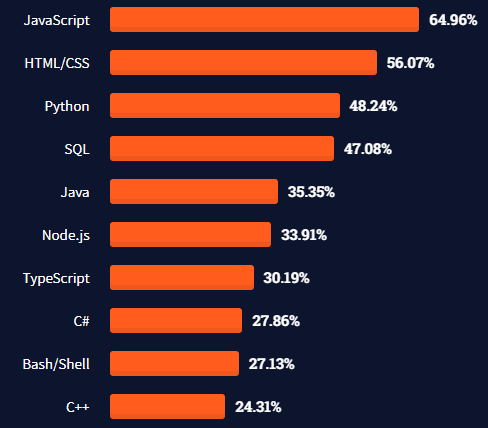
\includegraphics[width=0.5\textwidth]{figures/most_used_2021}
	}\\
\subfloat[Most loved and dreaded programming languages.\label{subfig-2:loved_dreaded}]{%
	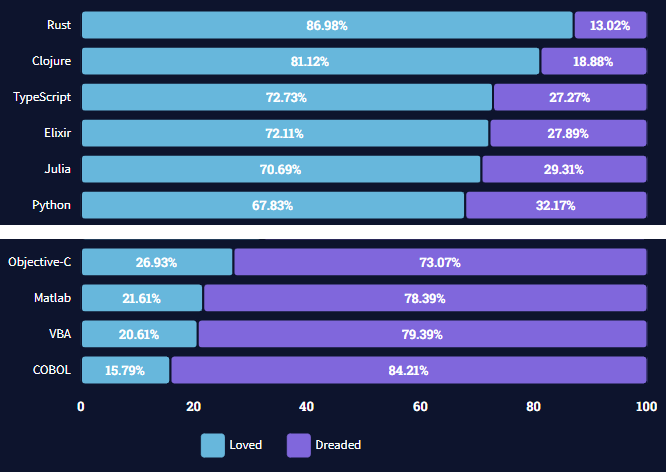
\includegraphics[width=0.7\textwidth]{figures/most_loved_dreaded_2021}
	}
\caption{Results from 2021 Stack Overflow survey.}
\label{fig:dummy}
\end{figure}

\subsection{Why \texttt{python}}

Assuming to have to simulate quantitative strategies for derivatives using plain statistics (no Machine Learning techniques involved), the typical step you have to take is to iterate a large number of times on quite big data sets (e.g. million of records data sets per asset).

It is then needed a programming language that could deal easily and without efforts with large data sets and was reasonably fast (do not consider for the moment integration with AI libraries).

Let's look at the possible alternatives to \texttt{python} for this typical endeavor.

\subsubsection{\texttt{R}}
\texttt{R} language has been the natural choice for doing statistics in the scientific community well before Data Science term was coined. While it is revolutionary and well suited to statistics, it is undoubtedly difficult to master and extremely inefficient in handling large data sets. 

Those are quite serious drawbacks, trading simulation usually requires large amounts of data, and if you need to start splitting it in advance or looking for alternative loading methods or simply the load process is complex it is worth to explore other options. 

This does not mean that \texttt{R} can not cope with it, it is just that it is not as easy and straightforward as for other languages. Data loading is an integral part of data analysis and it shall be provided out of the box.

\subsubsection{\texttt{C-C++}}
You can not be wrong with \texttt{C}. \texttt{C} is mature, it can do almost anything and it delivers very efficient code. \texttt{C} did not change substantially since its standard was formulated back in 1989. \texttt{C++} is also widely used and "extends" \texttt{C} with object-oriented paradigms.

The main problem with \texttt{C} is that it is "difficult" to do complex things with it. It shines for small algorithmic routines, and it is actually quite difficult to make it perform slow, but \emph{pointers} and their debugging can be challenging.
Usually while a project is getting bigger the timings and complexity to debugging it slowly but steadily grows.
Additionally, certain tasks which are trivial in other languages can be really challenging in \texttt{C}. 

\texttt{C/C++} language is widely used in High Frequency Trading (HFT) industry because it is a natural performer, but you must be ready to cope with longer projects that require skilled resources. It is the preferred choice when performance is paramount. 

\subsubsection{\texttt{Python} + \texttt{C}}
The logical to step to overcome \texttt{python} slowness is to replace its slow areas with \texttt{C}. 
The \texttt{C} routines when packed in \emph{shared libraries} can be invoked from \texttt{python} and this can be a win-win solution where you get the best of both worlds: speed from \texttt{C} and simplicity from \texttt{python}.

\subsubsection{\texttt{Fortran}}
\texttt{Fortran} is one of the oldest programming languages in service, \texttt{COBOL} aside. It was once the first choice for scientific and engineering analysis until the 90s and it has remained strong in computing demanding areas of the science.
\texttt{Fortran} is now a niche language but it still has an active community in many specialized fields such as high-energy physics, climate modeling, computational chemistry, structural engineering and molecular dynamics. Together with \texttt{C}, it is also the main programming language for super-computing. 

Modern \texttt{fortran} is quite easy to learn and master and often the algorithmic parts are easier to write than in \texttt{C}. \texttt{Fortran} also has some unique solutions to deal with array and structured data, which includes custom indexes, vector operations and simple ways to initialize variables and structures.

There are also some problems like bad integration of graphical tools and again debugging.  

\subsubsection{\texttt{Julia}}
\texttt{Julia} promises to deliver the simplicity of \texttt{python} with the speed of \texttt{C}.
The language is easy to learn and properly structured. The syntax is clear, it is not verbose and it is legible. Modules allow to adequately separate the code.

Certain aspects of the language were a bit puzzling at the beginning (i.e. mutable, variable sharing) but it is flexible enough to keep simpler tasks simple. Timestamp handling is pretty easy too, something which is relevant in this industry.
The overall times required to perform calculation are close to \texttt{C} since it compiles code in advance. The package installation service is also better incorporated than in \texttt{python} and it can be easily interfaced to it.

Using \texttt{julia} feels like you are an early adopter of a new technology and it might not be as stable and mature as other languages.

\section{What is \texttt{python} ?}
\label{what-is-python}

\texttt{Python} is a so called \emph{interpreted language}: it takes some code (a sequence of instructions), reads and executes it. This is different from other programming languages like \texttt{C} or \texttt{C++} which \emph{compile} code into a language that computers can understand directly (\emph{machine language}) (see Fig.~\ref{fig:compiled_vs_interpreted}).

\begin{figure}[htbp]
\centering
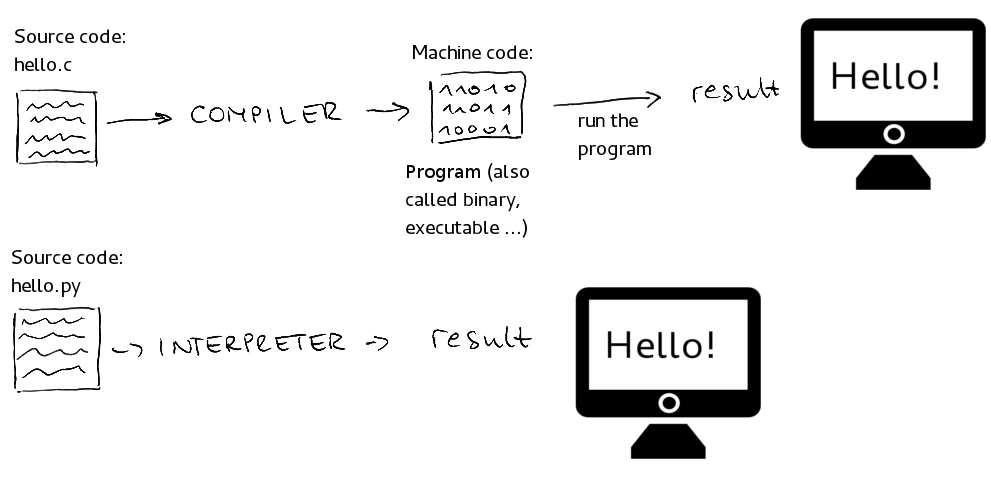
\includegraphics[width=0.7\linewidth]{figures/compiled_language}
\caption{Interpreted vs compiled language.}
\label{fig:compiled_vs_interpreted}
\end{figure}

As a result, \texttt{python} is essentially an \emph{interactive} programming language, which means you can program and see the results almost at the same time. This is very nice for a faster development since "compilation" time can be quite long (just to give an idea the compilation of our \texttt{C++} financial code takes more than one hour).
However there are drawbacks in term of performance, the \emph{translation} to machine language has to be done in real-time resulting in slower execution times (see Fig.~\ref{fig:compilation}).

\begin{figure}[htbp]
\centering
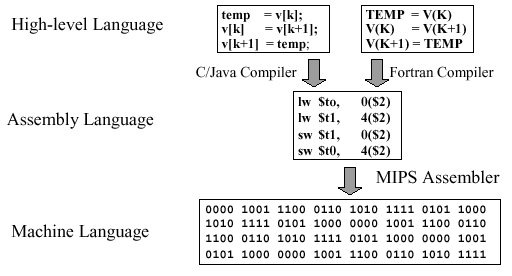
\includegraphics[width=0.5\linewidth]{figures/machine_language.png}
\caption{Human readable vs machine code}
\label{fig:compilation}
\end{figure}

In the next Chapters we'll take a quick tour of \texttt{python} and see the main features and characteristics of this programming language. Later on we will see how it can be useful to solve real-world financial problems.

First of all since \texttt{python}, as basically all programs, comes in different version and flavors we need to specify the particular one we are going to use~\cite{python_versions}.
The latest version (at the time I'm writing these pages) is \texttt{3.8.5}, however it is still not difficult to see older versions floating around (e.g. \texttt{2.7}).
This is because there are some big differences between \texttt{python 2.X} and \texttt{python 3.X} which prevent a sizable portion of \texttt{python 2} users to stick with it (consider that moving to \texttt{python 3} would require a large amount of work to adapt big projects).
In conclusion we will concentrate on \textbf{\texttt{python~3.X}}.

\section{\texttt{Python} Basics}
\label{python-basics}

Every language has \emph{keywords}, these are reserved words that have special meaning and tell the computer what to do. The most common one is \texttt{print}: it prints to screen whatever is specified between the parenthesis.
	
\begin{ipythonnon}
print ("Hello world !")
\end{ipythonnon}
\begin{ioutput}
Hello world !
\end{ioutput}
\begin{ipythonnon}
print ("Welcome")
print ("to")
print ("everybody")
\end{ipythonnon}
\begin{ioutput}
Welcome
to
everybody
\end{ioutput}

Good programming practice recommends to document the code you write (you will soon see that it is surprisingly easy to forget what you wanted to do in your code). In \texttt{python} you can add comments to code starting a line with a hash character (\#).

\begin{ipythonnon}
print ("Ciao") # this is a comment 
\end{ipythonnon}
\begin{ioutput}
Ciao
\end{ioutput}

\subsection{Variables}\label{variables}

If we want to really simplify what a program is and what it does, we may say that it is a series of instructions to be performed on various kind of data. Such data may be the name of a place, the height of a person or a series of prices taken by a trader. In programming, when we want to “label” a piece of information we give it a name and call it a variable, so we may say that a variable is a box which contains some kind of data.

More formally we can say that a variable is a computer memory location paired with a symbolic name, which contains some quantity of information referred to as a \emph{value} (e.g. a number, a string\ldots). 

A value is assigned to a variable with the equal operator (=) and printing a variable shows its content. 

\begin{figure}[htbp]
\centering
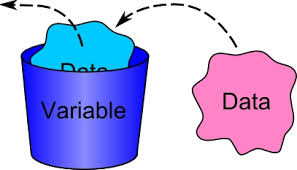
\includegraphics[width=0.35\linewidth]{figures/var1.jpeg}\\
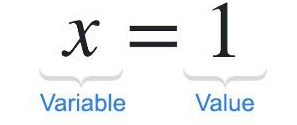
\includegraphics[width=0.35\linewidth]{figures/var2.jpeg}
\caption{Graphical representation of a variable.}
\end{figure}

\begin{ipythonnon}
x = 9 
print (x)
\end{ipythonnon}
\begin{ioutput}
9
\end{ioutput}
\begin{ipythonnon}
myphone = "MyFavourite Modile brand" 
print (myphone)
\end{ipythonnon}
\begin{ioutput}
MyFavourite Modile brand
\end{ioutput}

Another very useful keyword is \texttt{type}: it tells which kind of object is stored in a variable.

\begin{ipythonnon}
print (type(x))
print (type(myphone))
\end{ipythonnon}
\begin{ioutput}
<class 'int'>
<class 'str'>
\end{ioutput}

After their definitions \texttt{x} and \texttt{myphone} can be used as aliases for a number and a string and their content manipulated, for example:

\begin{ipythonnon}
print (x + 5)
\end{ipythonnon}
\begin{ioutput}
14
\end{ioutput}

There are rules that limit the variable naming possibilities, in particular they must:
\begin{itemize}
\tightlist
\item begin with a letter (\texttt{myphone}) or underscore (\texttt{\_myphone});
\item other characters can be letters, numbers or more underscores;
\item variable names are case-sensitive so \texttt{myphone} and \texttt{myPhone} are two distinct variables.
\end{itemize}

\textbf{Keywords, as said, are reserved words and as such cannot be used as variable names (e.g.~\texttt{print, type, for\ldots})}.

To use \textbf{good} variable names (and make your programs clearer and easier to read) always choose meaningful names instead of short names (i.e. \texttt{numberOfCakes} is much better than simply \texttt{n}), try to be consistent with your conventions (e.g.~choose once and for all between \texttt{number\_of\_cakes}, \texttt{numberofcakes} or \texttt{numberOfCakes}), usually begin a variable name with underscore (\_) only for a special case (will see later when this is necessary).

\subsection{Boolean Expressions}\label{boolean-expressions}

Boolean expressions evaluate to \texttt{True} or \texttt{False} only. This type
of expressions usually involve logical or comparison operators like \texttt{or}, \texttt{and}, $\geq$ (greater-than), $\leq$ (less-than)\ldots
The equal-to Boolean operator symbol is a double equal symbols (\texttt{==}), to not be confused with the assignment operator we have seen before made of a single equal symbol (\texttt{=}). With the first we compare two variables, with the second we associate a value to a variable.

Let's see some example. The following expression answers the question is 1 equal to 2:

\begin{ipythonnon}
1 == 2
\end{ipythonnon}
\begin{ioutput}
False
\end{ioutput}

Here another example using the not equal operator (\texttt{!=}):

\begin{ipythonnon}
1 != 2
\end{ipythonnon}
\begin{ioutput}
True
\end{ioutput}
\begin{ipythonnon}
2 < 2
\end{ipythonnon}
\begin{ioutput}
False
\end{ioutput}
\begin{ipythonnon}
2 <= 2 # in this case we allow the numbers to be equal too 
\end{ipythonnon}
\begin{ioutput}
True
\end{ioutput}
\begin{ipythonnon}
print (x)
15 <= x and x <= 20 # this expression could also be written as 15 <= x <= 20
\end{ipythonnon}
\begin{ioutput}
11
False
\end{ioutput}
\begin{ipythonnon}
15 <= x or x <= 20 
\end{ipythonnon}
\begin{ioutput}
True
\end{ioutput}
\begin{ipythonnon}
not (x > 20) # the not keyword negates the following expression 
\end{ipythonnon}
\begin{ioutput}
True
\end{ioutput}

\subsection{String Expressions}\label{string-expressions}

A string is a sequence of characters (letters, digits, spaces, punctuation\ldots). There are many operations that can be performed on strings, like for example concatenate (with \texttt{+} operator), truncate, replace characters\ldots

\begin{ipythonnon}
mystring = "some text with punctuation, spaces and digits 10" 
mystring.replace("s", "z")
\end{ipythonnon}
\begin{ioutput}
'zome text with punctuation, zpacez and digitz 10'
\end{ioutput}

\begin{ipythonnon}
"abc" + "def" # it is possible to concatenate strings with + 
\end{ipythonnon}
\begin{ioutput}
'abcdef'
\end{ioutput}

\begin{ipythonnon}
"The number " + 4 + " is my favorite number"
# this causes an error since we are trying to concatenate a string
# with a number so two different kind of objects
\end{ipythonnon}
\begin{ioutput} 
Traceback (most recent call last):
  File "<stdin>", line 1, in <module>
TypeError: must be str, not int
\end{ioutput}

This is the first time we make a mistake so that the \texttt{python} interpreter returns an error. We will discuss more deeply errors and their management in a later Section. 
For the moment it is enough to know that to avoid this particular error is possible to \textbf{cast} an object to a different type which means to convert an object to a different type. In this case we can \emph{force} the number four to be represented as a string with the \texttt{str()} function:

\begin{ipythonnon}
"The number " + str(4) + " is my favorite number"
\end{ipythonnon}
\begin{ioutput}
'The number 4 is my favorite number'
\end{ioutput}

\begin{ipythonnon}
print (type(3.4)) 
print (type(str(3.4)))
\end{ipythonnon}
\begin{ioutput}
<class 'float'>
<class 'str'>	
\end{ioutput}

In this simple case everything worked fine but type casting is not always possible: for example a number can be converted to a string (e.g. from the integer 4 to the actual symbol "4") but the opposite is not possible (e.g. cannot convert the string "matteo" to a meaningful number). In this second case we can try to use the function \texttt{int()} to convert a string to an integer.

\begin{ipythonnon}
int("matteo")
\end{ipythonnon}
\begin{ioutput}
Traceback (most recent call last):
  File "<stdin>", line 1, in <module>
ValueError: invalid literal for int() with base 10: 'matteo'
\end{ioutput}

\begin{ipythonnon}
int("4") 
\end{ipythonnon}
\begin{ioutput}
4
\end{ioutput}

\subsubsection{Pretty String Formatting}
In order to get prettier strings than those obtained just concatenating with the + operator, \texttt{python} allows to format text using the following syntax: \texttt{f"text \{var1\} other text \{var2\}"}.
This is not just a mannerism, for example we will see that it may be very useful to represent prices with the correct number of significant digits.

Using optional characters inside the curly brackets can determine the resulting format, for example\texttt{f"\{var:.1f\}"} means that this variable is a float number and that has to be printed with only one digit only after the decimal separator. 

\begin{ipythonnon}
c = 299792.458
print (f"The speed of light is about {c:.1f} km/s")	
\end{ipythonnon}
\begin{ioutput}
The speed of light is about 299792.5 km/s
\end{ioutput}

In addition to rounding formatted string can handle 0-padding of numbers, left or right alignment and so on. For a complete list of the available features please refer to \href{https://docs.python.org/3/tutorial/inputoutput.html}{Input and Output}.

\subsection{Mathematical Expressions}\label{mathematical-expressions}

Below few examples of the basic mathematical expressions available in \texttt{python}.

\begin{ipythonnon}
print (1 + 2)	
\end{ipythonnon}
\begin{ioutput}
3
\end{ioutput}

\begin{ipythonnon}
print (40 - 5)	
\end{ipythonnon}
\begin{ioutput}
35
\end{ioutput}

\begin{ipythonnon}
print (x * 20) # remember that x is equal to 9
\end{ipythonnon}
\begin{ioutput}
180	
\end{ioutput}

\begin{ipythonnon}
print (x / 4)
\end{ipythonnon}
\begin{ioutput}
2.25
\end{ioutput}

\begin{ipythonnon}
print (type(2.25))
\end{ipythonnon}
\begin{ioutput}
<class 'float'>	
\end{ioutput}

\begin{ipythonnon}
x // 4 # integer division, result will be truncated (no rounding)
       # 11 / 3 = 3.66666, 11 // 3 = 3
\end{ipythonnon}
\begin{ioutput}
2
\end{ioutput}

\begin{ipythonnon}
y = 3
print (x**y) # x to the power of y 	
\end{ipythonnon}
\begin{ioutput}
729
\end{ioutput}

\begin{ipythonnon}
print (3*x + y)	
\end{ipythonnon}
\begin{ioutput}
36	
\end{ioutput}

As an example of variable manipulation let's try to increment \texttt{x} by 1 and save the result again in \texttt{x}.

\begin{ipythonnon}
print (x)
x = x + 1
print (x)	
\end{ipythonnon}
\begin{ioutput}
15
16
\end{ioutput}

Sometimes the increment of a variable plus the assignment to the same variable is written with a more compact syntax \texttt{x += 1} (this is also true for other operators e.g. \texttt{x *= 2}).

More complex mathematical functions are not directly available, let's see for example the logarithm:

\begin{ipythonnon}
log(3)
\end{ipythonnon}
\begin{ioutput}
Traceback (most recent call last):
  File "<stdin>", line 1, in <module>
NameError: name 'log' is not defined
\end{ioutput}

\section{Modules}\label{modules}

One very important feature of each language is the ability to reuse code among different programs, e.g. imagine how awful would be if you had to re-implement every time you need it a function to compute the logarithm.
Usually there are mechanisms that allow to collect useful routines in \emph{packages} (or \emph{libraries}, or \emph{modules}) so that later they can be called and used by any program may need them.

These collections of utilities in \texttt{python} are called \emph{modules} and each installation of this language brings with it a standard set of them. If you need more functionality, you can download more modules from the web (there are zillions out there~\cite{modules}, see Fig.~\ref{fig:fancy_module}) or if you are not satisfied with what you found you can write your own (which is one of the goals of this course).

Some examples of useful modules we are going to use are:

\begin{itemize}
\tightlist
\item Numpy - which provides matrix algebra functionality and much more;
\item Scipy - which provides a whole series of scientific computing
  functions;
\item Pandas - which provides tools for manipulating time series or data-set
  in general;
\item Matplotlib - for plotting graphs;
\item Jupyter - for notebooks like the one used in classroom.
\end{itemize}

\begin{figure}
\centering
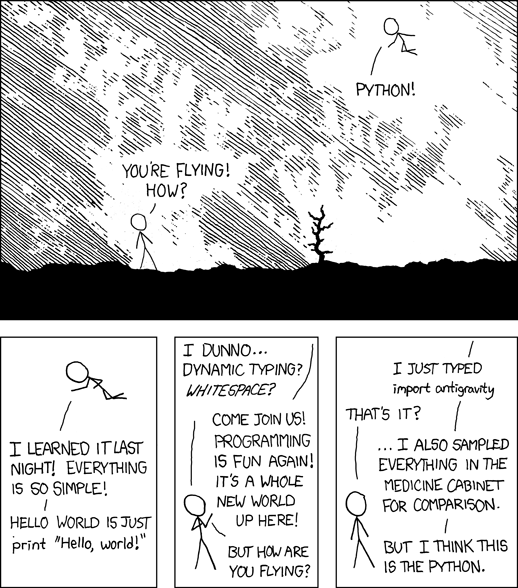
\includegraphics[width=0.5\linewidth]{figures/python.png}
\caption{\texttt{Python} has many modules for download on the web\ldots}
\label{fig:fancy_module}
\end{figure}

In Chapters~\ref{sec:datetime} and~\ref{sec:datamanip} we take a closer look at three modules which are particularly useful in financial analysis.

Notice that not all the modules are installed in your system with a standard \texttt{python} installation. In case you want to use one that is not available you can get it using the \texttt{pip} utility
\begin{ioutput}
pip install tensorflow
\end{ioutput}
Optionally it is possible to specify the exact version of the package that is needed like this
\begin{ioutput}
pip install tensorflow==3.0.1
\end{ioutput}
The command \texttt{pip} offers other useful options like to list the current installed packages
\begin{ioutput}
pip list
\end{ioutput}
Saving the output of the previous command to a file allows to later install at once all the listed packages to replicate a particular \texttt{python} environment

\begin{ioutput}
pip install -r pkg_list.txt
\end{ioutput}

Note that if you want to install a package in \texttt{Colab} just prepend an exclamation mark to the previous commands. 

In order to load a module in a \texttt{python} program you have to use the \texttt{import} keyword.
If a module name is long or awkward it is possible to define an alias with \texttt{import matplotlib.pyplot as plt}. To inspect a module, to understand which are its functionalities, it can be used either \texttt{help} and \texttt{dir} keywords: the first writes a help message which usually describes the functionalities of the module, the latter systematically lists all the available functions of a module.
\textbf{In order to access a function of a module you have to use the dot (\texttt{.}) operator: \texttt{module-name.function-name}.}

The \texttt{math} module implements the most common mathematical functions, let's see an example. 

\begin{ipythonnon}
import math
dir(math)
\end{ipythonnon}
\begin{ioutput}
['\_\_doc\_\_',
 '\_\_loader\_\_',
 '\_\_name\_\_',
 '\_\_package\_\_',
 '\_\_spec\_\_',
 'acos',
 'acosh',
 'asin',
 'asinh',
 'atan',
 'atan2',
 'atanh',
 ...
\end{ioutput}

\begin{ipythonnon}
help(math)
\end{ipythonnon}
\begin{ioutput}
Help on module math:

NAME
math

MODULE REFERENCE
https://docs.python.org/3.6/library/math

The following documentation is automatically generated from the Python
source files.  It may be incomplete, incorrect or include features that
are considered implementation detail and may vary between Python
implementations.  When in doubt, consult the module reference at the
location listed above.

DESCRIPTION
This module is always available.  It provides access to the
mathematical functions defined by the C standard.

FUNCTIONS
acos(...)
acos(x)

Return the arc cosine (measured in radians) of x.
...
\end{ioutput}

\begin{ipythonnon}
print (math.log(3))
\end{ipythonnon}
\begin{ioutput}
1.0986122886681098	
\end{ioutput}

\begin{ipythonnon}
print (math.exp(3))
\end{ipythonnon}
\begin{ioutput}
20.085536923187668	
\end{ioutput}

\begin{ipythonnon}
print (type(math.log)) # yet another type: builtin function
print (type(math.log(3)))
\end{ipythonnon}
\begin{ioutput}
<class 'builtin\_function\_or\_method'>
<class 'float'>	
\end{ioutput}

If you want to avoid to type \texttt{math.} every time you compute a logarithm or an exponential, it is possible to import only the needed functions from the module using the following syntax:

\begin{ipythonnon}
from math import log, exp

print (log(3))
print (exp(3))
\end{ipythonnon}
\begin{ioutput}
1.0986122886681098
20.085536923187668	
\end{ioutput}

As an example let's compute the interest rate $r$ that produces a return $R$ of 11000 EUR when investing 10000 EUR for 2 years:
\begin{equation*}
R = N\mathrm{e}^{r\tau} \implies r = \frac{1}{\tau} \mathrm{log}(\frac{R}{N})
\end{equation*}

\begin{ipythonnon}
rate = (1/2)*log(11000/10000)
print (rate)
\end{ipythonnon}
\begin{ioutput}
0.04765508990216247	
\end{ioutput}

\subsection{\texttt{finmarkets} Module}

Throughout this lectures many \texttt{python} financial applications will be reviewed. All code has been collected for simplicity into a \texttt{python} module called \texttt{finmarkets}. 

The module is currently in the \emph{test} repository of PyPi, the official collection of \texttt{python} modules. To install it in your working area you can still use \texttt{pip} but an additional option is needed 
\begin{ioutput}
pip install --index-url https://test.pypi.org/simple finmarkets
\end{ioutput}
	
Later you can access the code like all the other modules

\begin{ipythonnon}
from finmarkets import DiscountCurve
\end{ipythonnon}

\section{Indented Blocks and Conditionals}
\label{indented-blocks-and-the-ttifelse-statement}

Unlike other languages which uses parenthesis to isolate blocks of code \texttt{python} uses \emph{indentation}. A first example of this peculiarity is given by conditional statements (i.e. \texttt{if/elif/else}). Such commands allow to dynamically run different blocks of code based on conditions. For example in the following we print different statements according to the value of \texttt{x}, note that the block of code to be run according each condition is shifted (i.e. indented) with respect to the rest of the code:

\begin{ipythonnon}
print (x)
if x == 1:
	print ("This will not be printed")
elif x == 15:
	print ("This will not be printed either")
else:
	print ("This *will* be printed")
\end{ipythonnon}
\begin{ioutput}
16
This *will* be printed	
\end{ioutput}

If by mistake the indentation of a block is missing an exception is raised:

\begin{ipythonnon}
if x == 1:
    print ("This will not be printed")
elif x == 15:
    print ("This will not be printed either")
else:
   print ("This *will* be printed")
\end{ipythonnon}
\begin{ioutput}
  File "<stdin>", line 6
    print ("This will not be printed")
        ^
IndentationError: expected an indented block
\end{ioutput}

Below another example:
\begin{ipythonnon}
if x != 1:
    print ("x does not equal 1")
\end{ipythonnon}
\begin{ioutput}
x does not equal to 1	
\end{ioutput}

Just for comparison this is the same code written in \texttt{C++}:

\begin{lstlisting}[style=mycpp]
if (x == 1) {
 std::cout << "This will not be printed" << std::endl;
} else if (x == 15) {
     std::cout << "This will not be printed either" << std::endl;
} else {
   std::cout << "This *will* be printed" << std::endl;
}
\end{lstlisting}

Notice how indentation doesn't matter at all here since the blocks are enclosed and defined by the brackets.

\section{Loops}\label{loops}

Another very important feature of a language is the ability to repeatedly run the same block of code many times. This is called looping and in \texttt{python} can be done with \texttt{for} or \texttt{while} keywords.

\subsection{\texttt{for}}\label{for}

In a \texttt{for} loop we specify the set (or interval) over which we want to loop and a variable will assume all the values in that set (or interval). For example let's assume we want to print all the numbers between 25 and 30 (excluded) 

\begin{ipythonnon}
for i in range(25, 30):
    print (i)	
\end{ipythonnon}
\begin{ioutput}
25
26
27
28
29	
\end{ioutput}
\noindent
where the keyword \texttt{range} returns the list of integers between the specified limits, if the first limit is not specified 0 is assumed.
At each cycle of the loop the variable \texttt{i} takes one of the values between 25 and 29. 

With \texttt{range} it is also possible to specify the step, so that the loop can jump every 2 units or to go in descending order:

\begin{ipythonnon}
for i in range(30, 25, -1):
    print (i)	
\end{ipythonnon}
\begin{ioutput}
30
29
28
27
26	
\end{ioutput}

If it is needed to skip values in the loop the \texttt{continue} keyword can be used; in the code below 5 is actually not printed since it has been skipped by the condition executing \texttt{continue}:

\begin{ipythonnon}
for i in range(10):
    if i == 5:
        continue
    print (i)	
\end{ipythonnon}
\begin{ioutput}
0
1
2
3
4
6
7
8
9	
\end{ioutput}

Instead of using \texttt{range} it is possible to specify directly the set of looping values:

\begin{ipythonnon}
for i in (4, 6, 10, 20):
    print (i)	
\end{ipythonnon}
\begin{ioutput}
4
6
10
20	
\end{ioutput}

Finally looping on a string actually means to loop on each single character:
 
\begin{ipythonnon}
phrase = "how to loop over a string"
for c in phrase:
    print(c) 	
\end{ipythonnon}
\begin{ioutput}
h
o
w

t
o
...
\end{ioutput}
 
\subsection{\texttt{while}}\label{while}

The \texttt{while} statement repeats the same block of code until a condition is met. For example in the following code, the block is run until \texttt{x} squared is less than 50. At the beginning \texttt{x=1} and at each iteration we increment it by 1 "while" the condition is \texttt{True} (it should stop when \texttt{x}$> 7$ because it is the last squared lower than 50):

\begin{ipythonnon}
x = 1
while x**2 < 50:
    print (x)
    x += 1	
\end{ipythonnon}
\begin{ioutput}
1
2
3
4
5
6
7	
\end{ioutput}

It is possible to exit prematurely from a \texttt{while} loop using the \texttt{break} keyword. In this case the while-condition is simply \texttt{True} so the code would run forever unless we set an exit strategy.

\begin{ipythonnon}
x = 1
while True:
    if x**2 > 50:
        break
    print (x)
    x += 1	
\end{ipythonnon}
\begin{ioutput}
1
2
3
4
5
6
7	
\end{ioutput}

\section{Errors and Exceptions}
In the previous Sections we have already found a couple of examples with errors. Here we are going to look deeply what they are and how can be managed. There are (at least) two distinguishable kinds of errors:  \emph{syntax errors} and \emph{exceptions}.

\subsection{Syntax Errors}
Syntax errors are perhaps the most common kind of complaint you get while you are still learning \texttt{python}.

\begin{ipythonnon}
while True
    print ("Hello world")
\end{ipythonnon}
\begin{ioutput}
  File "<stdin>", line 1
    while True print('Hello world')
               ^
SyntaxError: invalid syntax
\end{ioutput}

The parser repeats the offending line and displays a little "arrow" pointing at the earliest point in the line where the error was detected. The error is caused by the token preceding the arrow: in the example, the error is detected at the function \texttt{print()}, since a colon (\texttt{:}) is missing before it. File name and line number are printed so you know where to look in case the input came from a script.

\subsection{Exceptions}
Even if a statement or expression is syntactically correct, it may cause an error when an attempt is made to execute it. Errors detected during execution are called exceptions and are not unconditionally fatal. Most exceptions are not handled by programs and result in error messages as shown here:

\begin{ipythonnon}
10 * (1/0)
\end{ipythonnon}
\begin{ioutput}
Traceback (most recent call last):
  File "<stdin>", line 1, in <module>
ZeroDivisionError: division by zero
\end{ioutput}

\begin{ipythonnon}
4 + spam*3
\end{ipythonnon}
\begin{ioutput}
Traceback (most recent call last):
  File "<stdin>", line 1, in <module>
NameError: name 'spam' is not defined
\end{ioutput}

\begin{ipythonnon}
'2' + 2
\end{ipythonnon}
\begin{ioutput}
Traceback (most recent call last):
  File "<stdin>", line 1, in <module>
TypeError: must be str, not int
\end{ioutput}

The last line of the error message indicates what happened. Exceptions come in different types, and the type is printed as part of the message: the types in the example are \texttt{ZeroDivisionError}, \texttt{NameError} and \texttt{TypeError}. The string printed as the exception type is the name of the exception that occurred. The rest of the line provides detail based on the type of exception and what caused it.

The preceding part of the error message shows the context where the exception occurred, in the form of a stack traceback listing source lines.

\subsection{Handling Exceptions}
It is possible to write programs that handle selected exceptions. Look at the following example, which asks the user for input until a valid integer has been entered, but allows the user to interrupt the program (e.g. using Control-C); note that a user-generated interruption is signaled by raising the \texttt{KeyboardInterrupt} exception.

\begin{ipythonnon}
while True: 
    try:
        x = int(input("Please enter a number: ")) 
        break
    except ValueError:
        print("Oops! That was no valid number. Try again...")
\end{ipythonnon}
\begin{ioutput}
Please enter a number: pippo
Oops!  That was no valid number.  Try again...

Please enter a number:
\end{ioutput}

The \texttt{try} statement works as follows: first, the try clause is executed. If no exception occurs, the except clause is skipped and execution of the \texttt{try} statement is finished.

If an exception occurs during execution of the try clause, the rest of the clause is skipped. Then if its type matches the exception named after the \texttt{except} keyword, the corresponding except clause is executed, and then execution continues after the \texttt{try} statement.

If an exception occurs which does not match the exception named in the except clause, it is passed on to outer \texttt{try} statements; if no handler is found, it is an un-handled exception and execution stops with a message as shown above.

A \texttt{try} statement may have more than one except clause, to specify handlers for different exceptions. At most one handler will be executed. Handlers only handle exceptions that occur in the corresponding try clause, not in other handlers of the same \texttt{try} statement.

\begin{ipythonnon}
except RuntimeError, TypeError, NameError:
    pass	
\end{ipythonnon}

The last except clause may omit the exception name(s), to serve as a wildcard. Use this with extreme caution, since it is easy to mask a real programming error in this way! 

\begin{ipythonnon}
import sys 

try:
    with open('myfile.txt') as f: 
        s = f.readline()
        i = int(s.strip()) 
except OSError as err:
    print(f"OS error: {err}") 
except ValueError:
    print("Could not convert data to an integer.") 
except:
    print("Unexpected error:", sys.exc_info()[0])
\end{ipythonnon}
\begin{ioutput}
OS error: [Errno 2] No such file or directory: 'myfile.txt'	
\end{ioutput}

\section{Assertions}
\texttt{Python} has a useful command called \texttt{assert} which can be used for checking that a given condition is satisfied, and it raises an exception if this is not true. This is clearly very important when debugging some code, it helps in searching for mistakes in the logic of an algorithm.

Below few examples of its usage. The following line does not cause an error, in fact it does nothing since 1 is lower than 2, hence the condition is met:

\lstinline[language=iPython]|assert 1 < 2|

\noindent
The next one instead causes an error (the condition is evaluated to false): 

\lstinline[language=iPython]|assert 1 > 2|

\noindent
\texttt{assert} can take a second optional argument with a message to display in case of failure.

\lstinline[language=iPython]|assert 1 > 2, "Two is greater than one"|

\section*{Exercises}
\begin{question}
What is the built-in function that \(\tt{python}\) uses to iterate over a number sequence ? Write an example that uses it.
\end{question}

\cprotEnv \begin{solution}
The built-in function used to iterate over a sequence of numbers is \(\tt{range}\). It returns a sequence of numbers taking three parameters that represents respectively the lower boundary of the sequence, the upper boundary of the sequence and the step. Note that the upper boundary is excluded from the sequence.

\begin{ipython}
for i in range(10, 20, 2):
    print (i)
\end{ipython}
\begin{ioutput}
10
12
14
16
18
\end{ioutput}
If just one parameter is passed the default lower boundary is 0 and the step is 1. 
\begin{ipython}
for i in range(5):
    print (i)
\end{ipython}
\begin{ioutput}    
0
1
2
3
4
\end{ioutput}
\end{solution}

\begin{question}
What is a string in \(\tt{python}\) ? Declare one string variable and try to manipulate it (concatenate, make uppercase, capitalize, replace characters, split...).
\end{question}

\cprotEnv \begin{solution}
A string is simply a sequence of characters.

\begin{ipython}
aString = "this is a string"
  
aString = aString + ", just an example"
print(aString)
\end{ipython}
\begin{ioutput}
'this is a string, just an example'
\end{ioutput}
\begin{ipython}
print(aString.upper())
\end{ipython}
\begin{ioutput}
'THIS IS A STRING, JUST AN EXAMPLE'
\end{ioutput}
\begin{ipython}
print(aString.capitalize())
\end{ipython}
\begin{ioutput}
'This is a string, just an example'
\end{ioutput}
\begin{ipython}
print(aString.replace("just an", "for"))
\end{ipython}
\begin{ioutput}
'this is a string, for example'
\end{ioutput}
\begin{ipython}
print(aString.split(","))
\end{ipython}
\begin{ioutput}
['this is a string', ' just an example']
\end{ioutput}
\begin{ipython}
if aString.endswith("example"):
    print("This string is really an example.")
else:
    print("This string is not an example.")
\end{ipython}
\begin{ioutput}
'This string is really an example.'
\end{ioutput}
\end{solution}

\begin{question}
What does the continue do in \(\tt{python}\) ? Show an example of its usage printing all the odd numbers between 0 and 10.
\end{question}

\cprotEnv \begin{solution}
\(\tt{continue}\) is used to skip cycles in for loops. Note that \% is the module operator, it returns the reminder of a division.

\begin{ipython}
for i in range(10):
    if i%2 == 0:
        continue
    else:
        print(i)
\end{ipython}
\begin{ioutput}    
1
3
5
7
9
\end{ioutput}
\end{solution}

\begin{question}
When should you use the break in \(\tt{python}\) ? Show an example of its usage.
\end{question}

\cprotEnv \begin{solution}
\(\tt{break}\) is the command used to interrupt a while loop even if the while condition is still satisfied.

\begin{ipython}
i = 0
while i < 11:
    if (i/2) > 3:
        break
    print(i)
    i += 1 
\end{ipython}
\begin{ioutput}    
0
1
2
3
4
5
6
\end{ioutput}
\end{solution}

\begin{question}
Which \(\tt{python}\) function will you use to convert a number to a string ? Show an example.
\end{question}

\cprotEnv \begin{solution}
\(\tt{str()}\) is the correct function to use in order to cast a number to a string.

\begin{ipython}
x = 2.34
print("This {} is of type {}".format(x, type(x)))
print("This {} is of type {}".format(str(x), type(str(x))))
\end{ipython}
\begin{ioutput}    
This 2.34 is of type <class 'float'>
This 2.34 is of type <class 'str'>
\end{ioutput}
\end{solution}

\begin{question}
Import the math module and compute the logarithm of 2.09, the exponential of 1.57 and the area of a circle of radius 6 cm (circle area = $\pi \cdot r^2$).
\end{question}

\cprotEnv \begin{solution}
\begin{ipython}
import math

print ("log(2.09) = {}".format(math.log(2.09))
print ("exp(1.57) = {}".format(math.exp(1.57))
print ("area of a circle (R=6cm) is about {} cm2".format(math.pi*6*6))
\end{ipython}
\begin{ioutput}    
log(2.09) = 0.7371640659767196
exp(1.57) = 4.806648193775178
area of circle (R=6cm) is about 113.10 cm2
\end{ioutput}
\end{solution}

\cprotEnv \begin{question}
\label{ex:BS1}
Given the following variables write out the Black Scholes formula and save the value of a call in a variable named `call\_price' and the value of a put in a variable named `put\_price'.

\begin{ipython}
S_t = 800.0 # spot price of the underlying
K = 600.0 # strike price
vol = 0.25 # volatility
r = 0.01 # interest rate
ttm = 0.5 # time to maturity, in years
\end{ipython}
\textbf{Hint:} remember that there are many modules available in \texttt{python} that let you save a lot of time. In this case we need the cumulative distribution function of the standard normal distribution which can be found in \texttt{scipy.stats} module, the name of the function is \texttt{norm}.
\end{question}

\cprotEnv \begin{solution}
The BS equation for the price of a call is:

\[ C(S, t) = S_tN(d_1)-Ke^{-r(T-t)}N(d_2) \]

where
\begin{itemize}
\item \(S_t\) is the spot price of the underlying
\item \(K\) is the strike price
\item \(r\) is the risk-free interest rate (expressed in terms of continuous compounding)
\item \(N(\cdot)\) is the cumulative distribution function of the standard normal distribution
\item \(T - t\) is the time to maturity
\item \(\sigma\) is the volatility of the underlying
\end{itemize}

\[\begin{split}
d_1 & = \cfrac{\mathrm{ln}(\cfrac{S_t}{K}) + (r + \cfrac{1}{2}\sigma^{2})(T-t)}{\sigma\sqrt{T-t}}\\ \\
d_2 & = d_1 - \sigma\sqrt{T-t}\\
\end{split}\]

\begin{ipython}
from math import log, exp, sqrt
# You'll need the Gaussian cumulative distribution function 
from scipy.stats import norm

S_t = 800.0 
ttm = 0.5
K = 600.0 
vol = 0.25 
r = 0.01

d1_num = (log(S_t/K)+(r+0.5*pow(vol, 2))*ttm) 
d1_den = vol*sqrt(ttm)
d1 = d1_num /d1_den
d2 = d1 - d1_den

call_price = S_t * norm.cdf(d1) - K * exp(-r*ttm)*norm.cdf(d2)
put_price = - S_t * norm.cdf(-d1) + K * exp(-r*ttm)*norm.cdf(-d2)
print ("{:.3f} {:.3f}".format(call_price, put_price)) 
\end{ipython}
\begin{ioutput}    
205.472 2.480
\end{ioutput}
\end{solution}


\chapter{Data Containers}
\label{sec:datacontainer}

In this Chapter the container types available in \texttt{python} are reviewed.

\section{Lists}
\label{lists}

A list in \texttt{python} is a container that is a \emph{mutable}, ordered sequence of elements. Each element or value that is inside of a list is called an \emph{item}. Each item can be accessed using square brackets notation, \texttt{alist[index]}, where \texttt{index} is the position of the item in the list.
Remember that, list indexing is zero-based so the first element has index 0 actually. A list is considered mutable since you can add, remove or update the items in it. Ordered instead means that items are kept in the same order they have been added to. Lists can be created by enclosing in square brackets the comma-separated list of the items or using the \texttt{list()} operator.

\begin{ipython}
mylist = list([21, 32, 15])
mylist = [21, 32, 15]

print(mylist)
print (type(mylist))
\end{ipython}
\begin{ioutput}
[21, 32, 15]
<class 'list'>
\end{ioutput}

\begin{ipython}
print (mylist[0])
\end{ipython}
\begin{ioutput}
21
\end{ioutput}

If you have a list of lists (i.e. a 2-dimensional list) you can use the square brackets
multiple times to access the inner elements:
\begin{ipython}
alist = [[1,2], [3,4], [5,6]]
print (alist[1][1]) # first [1] returns [3,4], second returns 4                 
\end{ipython}  

The number of elements in a list is counted using the function \texttt{len()}:
\begin{ipython}
print(len(mylist))
\end{ipython}
\begin{ioutput}
3
\end{ioutput}

Looping on list items can be achieved in two ways: using directly the list or by index:

\begin{ipython}
print ("Loop using the list itself:")
for i in mylist:
    print (i)
\end{ipython}
\begin{ioutput}
Loop using the list itself:
21
32
15
\end{ioutput}
\begin{ipython}
print ("Loop by index:")
for i in range(len(mylist)): # len returns number of items in the list
    print (i)
\end{ipython}
\begin{ioutput}
Loop by index:
21
32
15
\end{ioutput}

With the \texttt{enumerate} function is actually possible to do both at the same time since it returns two values, the index of the item and its value, so in the example below, \texttt{i} will take the item indices while \texttt{item} the item value itself:

\begin{ipython}
for i, item in enumerate(mylist):
    print (i, item)
\end{ipython}
\begin{ioutput}
0 21
1 74
2 85
3 15
4 188
\end{ioutput}

Since a list is mutable its items can be changed dynamically:

\begin{ipython}
mylist[1] = 74 # we can change list items since it's *mutable*
print (mylist)
\end{ipython}
\begin{ioutput}
[21, 74, 15]
\end{ioutput}

With \texttt{append} an item is added at the end, while with \texttt{insert} an 
item can be added in a specified position:

\begin{ipython}
mylist.append(188) # append add an item at the end of the list
print (mylist)
\end{ipython}
\begin{ioutput}
[21, 74, 15, 188]
\end{ioutput}
\begin{ipython}
mylist.insert(2, 85) # insert an item in the desired position
                     # (2 in this example)
print (mylist)
\end{ipython}
\begin{ioutput}
[21, 74, 85, 15, 188]
\end{ioutput}

To append multiple values at once to a list a loop can be used but \texttt{python} offers a single line way of doing it: \texttt{[i*2 for i in range(10)]}. This syntax is called \emph{list comprehension}.

Accessing items outside the list range gives an error:

\begin{ipython}
mylist[10] # error ! it doesn't exists, the list has only 3
           # elements, so the last is item 2
\end{ipython}
\begin{ioutput}
Traceback (most recent call last):
  File "<stdin>", line 1, in <module>
IndexError: list index out of range
\end{ioutput}

Read carefully the error messages usually they are very explicative and can help a lot 
in \emph{debugging} (i.e. finding mistakes) in your programs.

There are two more nice features of \texttt{python} indexing:

\begin{itemize}
\tightlist
\item negative indices are like positive ones except that they starts from the last element;
\item \emph{slicing} which allows to specify a range of indices to select more items at once 
(if the first or last limits are missing slicing will start from the first or end 
with last index respectively).
\end{itemize}

\begin{ipython}
print ("negative index -1 returns the last element:", mylist[-1])
print ("slice [1:3] returns items 1st and 2nd:", mylist[0:3])
print ("slice [:2] returns items 0th and 1st:", mylist[:2])
print ("slice [2:] returns items between the 2nd and the last:", mylist[2:])
\end{ipython}
\begin{ioutput}
negative index -1 returns the last element: 188
slice [1:3] returns items 1st and 2nd: [21, 74, 85]
slice [:2] returns items 0th and 1st: [21, 74]
slice [2:] returns items between the 2nd and the last: [85, 15, 188]
\end{ioutput}
\noindent
Needless to say that slicing with \texttt{[:]} returns the entire list.

It is worth mentioning that a list doesn't have to be populated with the same kind of objects (list indices are instead always integers).

\begin{ipython}
mixedlist = [1, 2, "b", math.sqrt]
print (mixedlist)
\end{ipython}
\begin{ioutput}
[1, 2, 'b', <built-in function sqrt>]
\end{ioutput}

\begin{ipython}
print (mixedlist['k'])
\end{ipython}
\begin{ioutput}
Traceback (most recent call last):
  File "<stdin>", line 1, in <module>
TypeError: list indices must be integers or slices, not str
\end{ioutput}

A complete list of the commands available for a list can be shown with \texttt{dir(list)}:

\begin{ipython}
dir(list)
\end{ipython}
\begin{ioutput}
[...
 'append',
 'clear',
 'copy',
 'count',
 'extend',
 'index',
 'insert',
 'pop',
 'remove',
 'reverse',
 'sort']
\end{ioutput}

Their meaning is pretty clear, so for example \texttt{sort} re-order the items according to a custom criteria or \texttt{index(item)} return the index of the specified item.

\section{Dictionaries}\label{dictionaries}

A we have seen lists are ordered collections of elements and as such we can say that map integers (the index of each item) to values (any kind of \texttt{python} object). \emph{Dictionaries} generalize such a concept being containers which map \emph{keys} (\textbf{almost} any kind of \texttt{python} object) to values (any kind of \texttt{python} object).

In our previous section we had:
\[
\begin{matrix} 
0~(\textrm{0th item})& \rightarrow& 21\\
1~(\textrm{1st item})& \rightarrow& 74\\
2~(\textrm{2nd item})& \rightarrow& 85\\ 
&\cdots&  
\end{matrix}
\]
With a dictionary we can have something like this:
\[
\begin{matrix}
"apple" (\textrm{key})&\rightarrow& 4 \\
"banana" (\textrm{key})& \rightarrow& 5 \\
&\cdots&
\end{matrix}
\]
As we will see dictionaries are very flexible and will be very useful to represent complex data structures.

Dictionaries can be created by enclosing in curly brackets the comma-separated list of key-value pairs (key and value are separated by a \texttt{:} (colon)), or using the \texttt{dict()} operator. In lists we could access items by index, here we do it by key still using the square brackets. Trying to access not existing keys results in error, but we can check if a key exists with the \texttt{in} operator. As before, if a dictionary contains other dictionaries or lists, the square brackets can be applied repeatedly to access the inner items.

\begin{ipython}
adict = {"apple": 4, "banana": 5}
print (adict["apple"])
\end{ipython}
\begin{ioutput}
4
\end{ioutput}

\begin{ipython}
adict["pear"] # error !
\end{ipython}
\begin{ioutput}
Traceback (most recent call last):
  File "<stdin>", line 1, in <module>
KeyError: 'pear'
\end{ioutput}

\begin{ipython}
'pear' in adict # indeed
\end{ipython}
\begin{ioutput}
False
\end{ioutput}

The items can be dynamically created or updated with the assignment \texttt{=} operator, while again \texttt{len()} returns the number of items in a dictionary.

\begin{ipython}
adict["banana"] = 2
adict["pear"] = 10

print (len(adict))
print (adict)
\end{ipython}
\begin{ioutput}
3
{'apple': 4, 'banana': 2, 'pear': 10}
\end{ioutput}

Dictionaries can be made of more complicated types than simple string and integers:

\begin{ipython}
adict[math.log] = math.exp
\end{ipython}

Also dictionaries can be created with the \emph{comprehension} syntax: \texttt{\{i:v for i, v in enumerate(["a", "b", "c"])\}}.

Looping over dictionary items can be done by key, by value or both: \texttt{.keys()} returns a list of keys, \texttt{.values()} returns a list of values and \texttt{.items()} a list of pairs key-value.

\begin{ipython}
print ("All keys: ", adict.keys())

for key in adict.keys():
    print (key)
\end{ipython}
\begin{ioutput}
All keys:  dict_keys(['apple', 'banana', 'pear', <built-in function log>])
apple
banana
pear
<built-in function log>
\end{ioutput}
\begin{ipython}
print ("All values: ", adict.values())

for value in adict.values():
    print (value)
\end{ipython}
\begin{ioutput}
All values:  dict_values([4, 2, 10, <built-in function exp>])
4
2
10
<built-in function exp>
\end{ioutput}
\begin{ipython}
print ("All key-value pairs: ", adict.items())

for key, value in adict.items():
    print (key, value)
\end{ipython}
\begin{ioutput}
All key-value pairs:  dict_items([('apple', 4), ('banana', 2), ('pear', 10),
(<built-in function log>, <built-in function exp>)])
apple 4
banana 2
pear 10
<built-in function log> <built-in function exp>
\end{ioutput}

To merge two dictionaries the function \texttt{update()} can be used, while with \texttt{del} it is possible to remove a key-value pair.

\begin{ipython}
del adict[math.log]
seconddict = {"watermelon": 0, "strawberry": 1}
adict.update(seconddict)
print (adict)
\end{ipython}
\begin{ioutput}
{'apple': 4, 'banana': 2, 'pear': 10, 'watermelon': 0, 'strawberry': 1}
\end{ioutput}

Again the complete list of dictionary functions can be shown with \texttt{dir}:

\begin{ipython}
dir(dict)
\end{ipython}
\begin{ioutput}
[...
 'clear',
 'copy',
 'fromkeys',
 'get',
 'items',
 'keys',
 'pop',
 'popitem',
 'setdefault',
 'update',
 'values']
\end{ioutput}

\section{Tuples}\label{tuples}

Tuples create a bit of confusion for beginners because they are very similar to lists 
but they have some subtle conceptual differences, see Fig.~\ref{fig:tuples}.
Nonetheless, tuples do appear when programming in \texttt{python} so it's important to know about them.

\begin{figure}[hb]
\centering
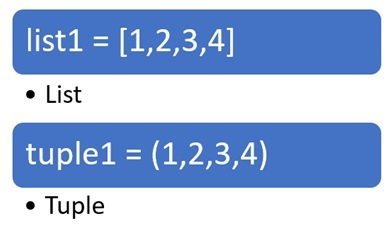
\includegraphics[width=0.5\textwidth]{figures/Difference-Between-List-and-Tuple-fig-1-2.jpg}
\caption{At first glance list and tuples look very similar, but they are not\ldots}
\label{fig:tuples}
\end{figure}

Like lists, tuples are containers of any type of object. Unlike lists though they are \emph{immutable} which means that once they have been created the content cannot be changed (i.e. no append, insert or delete of the elements). Furthermore since they are immutable they can be used as dictionary keys (lists cannot). To create a tuple the comma-separated list of items has to be enclosed in brackets, or the \texttt{tuple()} operator can be used. Accessing tuple items is done in exactly the same way as lists.

\begin{ipython}
atuple = (1, 2, 3)
print ("Length: {}".format(len(atuple)))
print ("First element: {}".format(atuple[0]))
print ("Last element: {}".format(atuple[-1]))
\end{ipython}
\begin{ioutput}
Length: 3
First element: 1
Last element: 3
\end{ioutput}

In the next snippet of code it is shown the so called unpacking which is another way to assign tuple values to variables.

\begin{ipython}
x, y, z = (10, 5, 12)
print ("coord: x={} y={} z={}".format(x, y, z))
\end{ipython}
\begin{ioutput}
coord: x=10 y=5 z=12
\end{ioutput}

If an tuple has just one element don't forget the comma at the end otherwise it will be 
treated as a single number.

\begin{ipython}
tuple2 = (1,)
print(type(tuple2))

tuple2 = (1)
print(type(tuple2))
\end{ipython}
\begin{ioutput}
<class 'tuple'>
<class 'int'>
\end{ioutput}

Since a tuple is immutable to add new elements it is necessary to create a new object:

\begin{ipython}
tuple1 = (1, 2, 3)
tuple2 = tuple1 + (4, 5)
print(tuple2)
\end{ipython}
\begin{ioutput}
(1,2,3,4,5)
\end{ioutput}

Finally, as already said tuples can be used as dictionary keys:

\begin{ipython}
d = {
	('Finance', 1): 'Room 8',
	('Finance', 2): 'Room 3',
	('Math', 1): 'Room 6',
	('Programming', 1): 'IT room'}
\end{ipython}

Below the full list of tuple functions:
\begin{ipython}
dir(dict)
\end{ipython}
\begin{ioutput}
[...
 'count',
 'index']
\end{ioutput}

\section{Exercises}
\begin{question}
What is a dictionary in \(\tt{python}\) programming language ? Create a dictionary, modify it and then print all its items.
\end{question}

\cprotEnv\begin{solution}
A dictionary is a container that maps a key (any object) to a value (any object), contrary to lists which map an integer (the index) to a value (any object).

\begin{ipython}
dictionary = {"calculus": 28, "physics":30, "chemistry":25}

dictionary["laboratory"] = 27
dictionary["chemistry"] = 24

print ("Exam\tVote")
for k, v in dictionary.items():
    print("{}:\t{}".format(k, v))
\end{ipython}
\begin{ioutput}
Exam            Vote
calculus:       28
physics:        30
chemistry:      24
laboratory:     27
\end{ioutput}
\end{solution}

\begin{question}
Write code which, given the following list 

\lstinline[language=iPython]|input\_list = [3, 5, 2, 1, 13, 5, 5, 1, 3, 4]|

\noindent
prints out the indices of every occurrence of \lstinline[language=iPython]|y=5|.
\end{question}

\cprotEnv\begin{solution}
\begin{ipython}
l = [3, 5, 2, 1, 13, 5, 5, 1, 3, 4]

for i in range(len(l)):
    if l[i] == y:
        print (i)
\end{ipython}
\begin{ioutput}
1
5
6
\end{ioutput}
Note that lists already have a way to get the occurrences of an item: \texttt{l.count(5)} would have done the job.
\end{solution}

\begin{question}
Write a \texttt{python} program to convert a list of tuples into a dictionary where the keys are the first elements of each tuples and the values the second.

\noindent
Input: \lstinline[language=iPython]|l = [("x", 1), ("x", 2), ("x", 3), ("y", 1), ("y", 2), ("z", 1)]|
\end{question}

\cprotEnv\begin{solution}
\begin{ipython}
l = [("x", 1), ("x", 2), ("x", 3), ("y", 1), ("y", 2), ("z", 1)]

d = {}
for item in l:
    d[item][0]] = item[1]
    
print(d)
\end{ipython}
\begin{ioutput}
{'x': 3, 'y': 2, 'z': 1}
\end{ioutput}
Note that there is just one occurrence of the key $\tt{x}$ and $\tt{y}$ because keys has to be unique and setting the same key to a different value simply overwrite the existing entry.
\end{solution}

\begin{question}
Write a \texttt{python} program to increment by 10 the last value of each tuples in a list.

\noindent
Input: \lstinline[language=iPython]|l = [(10, 20, 40), (40, 50, 60), (70, 80, 90)]|.
\end{question}

\cprotEnv\begin{solution}
\begin{ipython}
l = [(10, 20, 40), (40, 50, 60), (70, 80, 90)]

for i in range(len(l)):
    new_tuple = l[:-1] + [l[2] + 10]
    l[i] = new_tuple
    
print (l)
\end{ipython}
\begin{ioutput}
[(10, 20, 50), (40, 50, 70), (70, 80, 100)]
\end{ioutput}
\end{solution}

\begin{question}
Write a \texttt{python} program to count the elements in a list until an element is a tuple.

\noindent
Input:\lstinline[language=iPython]|l = [1, 5, 'a', (1, 2), 'test':1]|
\end{question}

\cprotEnv\begin{solution}
\begin{ipython}
l = [1, 5, 'a', (1, 2), 'test':1]

number_of_items = 0 
for item in l:
    if type(item) != 'tuple'{:}
        number_of_items += 1
    else:
        break
        
print("There are {} items before a tuple.".format(number_of_items))
\end{ipython}
\begin{ioutput}
\end{ioutput}
\end{solution}

\begin{question}
Write a \texttt{python} script to concatenate the following dictionaries to create a new single one.

\noindent 
Input:
\lstinline[language=iPython]|dic1 = \{1:10, 2:20\}; dic2 = \{3:30, 4:40\}; dic3 = \{5:50, 6:60\}|
\end{question}

\cprotEnv\begin{solution}
\begin{ipython}
dic1 = {1:10, 2:20}
dic2 = {3:30, 4:40}
dic3 = {5:50, 6:60}

dic_tot = dict()
dic_tot.update(dic1)
dic_tot.update(dic2)
dic_tot.update(dic3)

print(dic_tot)
\end{ipython}
\begin{ioutput}
{1: 10, 2: 20, 3: 30, 4: 40, 5: 50, 6: 60}
\end{ioutput}

An alternative and even more concise way using the \texttt{**} operator is the following:
\begin{ipython}
dic1 = {1:10, 2:20}
dic2 = {3:30, 4:40}
dic3 = {5:50, 6:60}

new_dic = {**dic1, **dic2, **dic3}
\end{ipython}
\end{solution}

\begin{question}
Write a \texttt{python} script to check whether a given key already exists in a dictionary.
\end{question}

\cprotEnv\begin{solution}
\begin{ipython}
dic = {"a":1, "b":2, "c":3}

print("z" in dic)
print("a" in dic)
\end{ipython}
\begin{ioutput}
False
True
\end{ioutput}
\end{solution}

\begin{question}
Write a \texttt{python} program to combine two dictionary adding values for common keys.

\noindent
Input: \lstinline[language=iPython]|d1 = \{'a':100, 'b':200, 'c':300\}; d2 = \{'a':300, 'b':200, 'd':400\}|
\end{question}

\cprotEnv\begin{solution}
\begin{ipython}
d1 = {'a':100, 'b':200, 'c':300}
d2 = {'a':300, 'b':200, 'd':400}

d = {}
d.update(d1)

for k in d2.keys():
    if k in d:
        d[k] = d[k] + d2[k]
    else:
        d[k] = d2[k]

print(d)
\end{ipython}
\begin{ioutput}
{'a': 400, 'b': 400, 'c': 300, 'd': 400}
\end{ioutput}
\end{solution}

\begin{question}
Given the following dictionary mapping currencies to 2-year zero coupon bond prices, build another dictionary mapping the same currencies to the corresponding annualized interest rates.

\lstinline[language=iPython]|d = {'EUR':0.9, 'CHF':1.005, 'USD':0.985, 'GBP':0.97}|
\end{question}

\cprotEnv\begin{solution}
The price of a n-years zero coupon bond is:

\[ P = \frac{M}{(1+r)^{n}} = M\cdot D \]
where $M$ is the value of the bond at the maturity, $r$ is the risk-free rate and $n$ is the number of years until maturity.
%Hence:

\[ D = \cfrac{1}{(1+r)^{n}} \implies r = \Big(\cfrac{1}{D}\Big)^{\cfrac{1}{n}} - 1\]

\begin{ipython}
# initialize an empty dictionary in which to store result
rates = {}

maturity = 2
discount_factors = {'EUR':0.9, 'CHF':1.005, 'USD':0.985, 'GBP':0.97}

# loop over the input dictionary to get the currencies
for currency, df in discount_factors.items():
    # calculate the rate and store it in the output dictionary
    rates[currency] = pow(1/df, 1/maturity) - 1
   
for r in rates.items():
    print(r)
\end{ipython}
\begin{ioutput}
('EUR', 0.05409255338945984)
('CHF', -0.002490663892367073)
('USD', 0.007585443719756668)
('GBP', 0.015346165133619083)
\end{ioutput}
\end{solution}

\begin{thebibliography}{9}
\bibitem{lists} \href{https://docs.python.org/3/tutorial/datastructures.html}{\emph{Data Structures, More on Lists}} [Online]
\bibitem{dictionaries} \href{https://realpython.com/python-dicts/}{\emph{Dictionaries in Python}}, Real Python [Online]
\bibitem{tuple} \href{https://www.programmareinpython.it/video-corso-python-base/14-liste-e-tuple/}{\emph{Liste e Tuple}}, Programmare in Python [Online]
\end{thebibliography}


\chapter{Date and Time}
\label{sec:datetime}

In this Chapter we take a little break and concentrate on a topic that it is not usually covered in a \texttt{python} review for beginners. However given its importance for financial computation the next paragraphs will be devoted to a close look up on the \texttt{datetime} module~\cite{bib:datetime}, whose usage will help in manipulating dates.

\section{Dates}\label{dates}

As said dates are not usually included in a standard \texttt{python} tutorial, however since they 
are pretty essential for finance we are going to cover this topic in some detail. 
In \texttt{python} the date utilities mainly lives in the \texttt{datetime} module. Briefly we are 
also going to show \texttt{relativedelta} from the \texttt{dateutil} module, which allows to 
add/subtract days/months/years to dates, in other words to make operations on them.

In this first example today's date is defined and with \texttt{relativedelta} two more dates are created 
adding two months and subtracting three days to the first one.

\begin{ipythonnon}
from datetime import date, datetime
from dateutil.relativedelta import relativedelta

date1 = date.today()
print(date1)

date2 = date.today() + relativedelta(months=2)
print(date2)

date3 = date.today() - relativedelta(days=3)
print(date3)
\end{ipythonnon}
\begin{ioutput}
2020-08-03
2020-10-03
2020-07-31
\end{ioutput}

There is another way of computing a new date: a one day delta is stored in a variable 
and today's date is moved by three days multiplying the defined delta by three.

\begin{ipythonnon}
one_day = relativedelta(days=1)
date.today() - 3 * one_day
\end{ipythonnon}
\begin{ioutput}
datetime.date(2020, 7, 31)
\end{ioutput}

Next, given two dates their difference is computed and expressed in number of days.

\begin{ipythonnon}
date1 = date(2019, 7, 2)
date2 = date(2019, 8, 16)
(date2 - date1).days
\end{ipythonnon}
\begin{ioutput}
45
\end{ioutput}

Dates can be converted to and from strings and a large variety of formats can be specified in this conversions. 
The format is determined by a string in which each character starting with \% represent an element 
of the date, e.g. \%Y year, \%d day, \%s seconds\ldots

Below dates to string conversion:

\begin{ipythonnon}
date1 = date(2019, 7, 2)
date1.strftime("%Y-%b-%d (%a)") # dates can formatted in many ways
                                # check the docs for more details
\end{ipythonnon}
\begin{ioutput}
'2019-Jul-02 (Tue)'
\end{ioutput}

And here, a string is converted to \texttt{datetime} object:

\begin{ipythonnon}
# a string can be converted to dates too
datetime.strptime('25 Aug 2019', "%d %b %Y").date()
\end{ipythonnon}
\begin{ioutput}
datetime.date(2019, 8, 25)
\end{ioutput}

Finally a last example showing how to get the week-day from a date:

\begin{ipythonnon}
date1.weekday() # 0 = Monday, ..., 6 = Sunday
\end{ipythonnon}
\begin{ioutput}
1
\end{ioutput}

\section{Date Utilities}

As said date management is very important in financial application, so the \texttt{finmarkets} module implements a couple of utilities to ease the work. 

\subsection{TimeInterval}

This simple function take in input a string representing a time interval (e.g. \texttt{"1y"} or \texttt{"5d"}) and convert it into a \texttt{relativedelta} object to be directly used with a \texttt{datetime.date}.

\pythoncodenon{code/datetime_timeinterval.py}
An example of usage is
\begin{ipythonnon}
from datetime import date
from finmarkets import TimeInterval

date = date(2024, 9, 6)
print (date)
print (date + TimeInterval("1y"))
print (date + TimeInterval("2m"))
\end{ipythonnon}
\begin{ioutput}
2024-09-06
2025-09-06
2024-11-06
\end{ioutput}

\subsection{Payment Dates Generator}

Another very useful tool available in \texttt{finmarkets} is the function \texttt{generate\_dates}. Its main purpose is to generate list of dates (e.g. payment dates), a task that we need to do often from now on. 
time
It takes in input: a starting date (the first date of the list), an end date which represents the "length" of the list (it can be an actual date or a \texttt{TimeInterval}) and frequency (12 months by default). Note that if the maturity is not a multiple of 12 months the last period will be truncated to the last date. It returns the list of dates.

\pythoncodenon{code/datetime_generate_dates.py}

\begin{ioutput}
[datetime.date(2020, 10, 20), datetime.date(2021, 10, 20), 
datetime.date(2022, 10, 20), datetime.date(2022, 11, 20)]
\end{ioutput}

\section*{Exercises}
\begin{question}
Write code that:

\begin{itemize}
\item print the day of the week of your birthday;
\item print the weekday of your birthdays for the next 120 years.
\end{itemize}
\end{question}

\begin{solution}
\end{solution}	
\begin{ipython}
import datetime

birthday = datetime.date(1974, 10, 20)
print (birthday.weekday()) # remember it starts form 0

6

from dateutil.relativedelta import relativedelta

for i in range(120):
    print ((birthday + relativedelta(years=i)).weekday())

6
0
2
3
4
5
0
1
2
3
4
...
\end{ipython}

\begin{question}
Write code to determine whether a given year is a leap year and test it with 1800, 1987 and 2020.

\noindent\textbf{Hint:} a leap year is divisible by 4, by 100 and by 400.
\end{question}

\begin{solution}
\end{solution}

\begin{ipython}
years = [1800, 1987, 2020]

for y in years:
    if y % 400 == 0:
        print ("{} is a leap year".format(y))
	elif y % 100 == 0:
        print ("{} is a leap year".format(y)) 
    elif y % 4 == 0:
        print ("{} is a leap year".format(y))
    else:
        print ("{} is NOT a leap year".format(y))

1800 is NOT a leap year
1987 is NOT a leap year
2020 is a leap year        
\end{ipython}  

\begin{question}
Write code to print next five days starting from today.
\end{question}

\begin{solution}
\end{solution}

\begin{ipython}
d = datetime.date.today()
for i in range(1, 6):
     print (d + relativedelta(days=i))

2020-08-04
2020-08-05
2020-08-06
2020-08-07
2020-08-08
\end{ipython}

\begin{question}
Build again dates as in exercise~\ref{dateex} (i.e. the weekday of your birthdays for the next 120 years) and count how many of your birthdays is a Monday, Tuesday, \ldots{} , Sunday until 120 years of age. Print out the result using a dictionary. (expected output something like: \texttt{\{6:\ 10,\ 0:\ 10,\ 2:\ 9,\ 3:\ 10,\ 4:\ 10,\ 5:\ 10,\ 1:\ 9\}})
\end{question}

\begin{solution}
\end{solution}

\begin{ipython}
import datetime
from dateutil.relativedelta import relativedelta

birthday = datetime.date(1974, 10, 20)
d = {}
for i in range(120):
    wd = (birthday + relativedelta(years=i)).weekday() 
    if wd in d.keys():
        d[wd] += 1
    else:
        d[wd] = 1
        
print (d)

{6: 17, 0: 18, 2: 17, 3: 17, 4: 17, 5: 17, 1: 17}
\end{ipython}

\begin{question}
Write an algorithm which takes in input a start date and a number of months, and returns a list of dates with \textbf{annual} frequency from the start date to the ending of the period after the specified number of months.

For example
\begin{itemize}
\item 2019-11-10 start date 12 months \(\rightarrow\) 2019-11-10, 2020-11-10
\item 2019-11-10 start date 24 months \(\rightarrow\) 2019-11-10, 2020-11-10, 2021-11-10
\end{itemize}

Note that if the number of months is not a multiple of 12, the last period should simply be shorter than 12 months. For example:

\begin{itemize}
\item 2019-11-10 start date 9 months \(\rightarrow\) 2019-11-10, 2020-08-10
\item 2019-11-10 start date 15 months \(\rightarrow\) 2019-11-10, 2020-11-10, 2021-02-10
\end{itemize}

%\begin{figure}
%  %\centering
%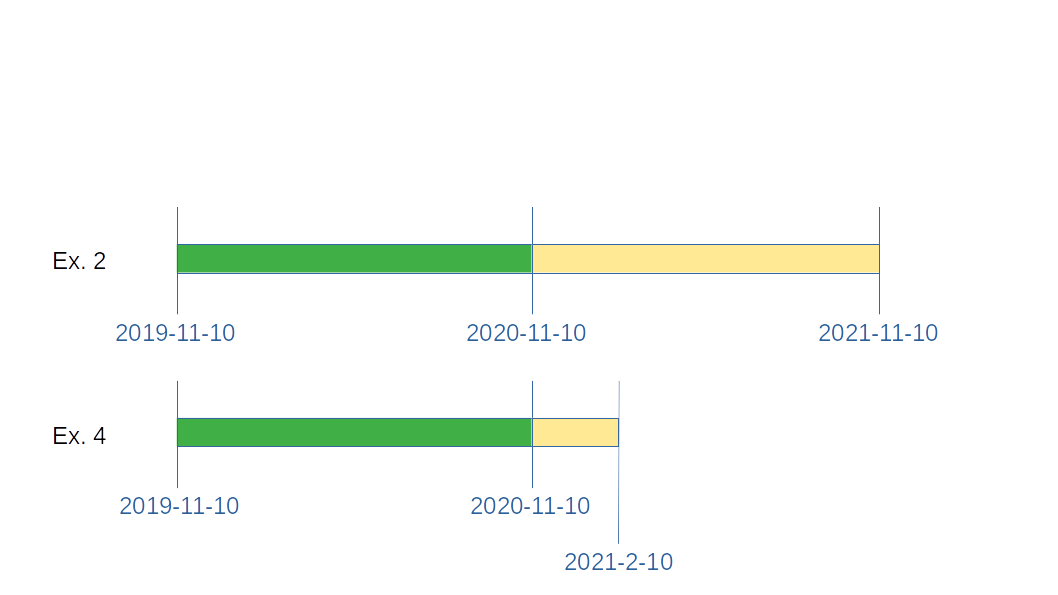
\includegraphics[width=0.8\linewidth]{time_flow.png}
%\end{figure}

%Here's some skeleton code to help you get started:
%
%\begin{Shaded}
%\begin{Highlighting}[]
%\ImportTok{from}\NormalTok{ dateutil }\ImportTok{import}\NormalTok{ relativedelta}
%
%\KeywordTok{def}\NormalTok{ generate_swap_dates(start_date, n_months):}
%\NormalTok{    dates }\OperatorTok{=}\NormalTok{ []}
%    \CommentTok{# your code here which adds all the relevant dates to the dates list}
%    \ControlFlowTok{return}\NormalTok{ dates}
%\end{Highlighting}
%\end{Shaded}
%
%\begin{Shaded}
%\begin{Highlighting}[]
%\CommentTok{# some tests to check if the function is working correctly}
%\ImportTok{from}\NormalTok{ datetime }\ImportTok{import}\NormalTok{ date}
%
%\ControlFlowTok{assert}\NormalTok{ generate_swap_dates(date(}\DecValTok{2019}\NormalTok{, }\DecValTok{11}\NormalTok{, }\DecValTok{10}\NormalTok{), }\DecValTok{12}\NormalTok{) }\OperatorTok{==}\NormalTok{ [date(}\DecValTok{2019}\NormalTok{, }\DecValTok{11}\NormalTok{, }\DecValTok{10}\NormalTok{), }
%\NormalTok{                                                       date(}\DecValTok{2020}\NormalTok{, }\DecValTok{11}\NormalTok{, }\DecValTok{10}\NormalTok{)]}
%\ControlFlowTok{assert}\NormalTok{ generate_swap_dates(date(}\DecValTok{2019}\NormalTok{, }\DecValTok{11}\NormalTok{, }\DecValTok{10}\NormalTok{), }\DecValTok{24}\NormalTok{) }\OperatorTok{==}\NormalTok{ [date(}\DecValTok{2019}\NormalTok{, }\DecValTok{11}\NormalTok{, }\DecValTok{10}\NormalTok{), }
%\NormalTok{                                                       date(}\DecValTok{2020}\NormalTok{, }\DecValTok{11}\NormalTok{, }\DecValTok{10}\NormalTok{), }
%\NormalTok{                                                       date(}\DecValTok{2021}\NormalTok{, }\DecValTok{11}\NormalTok{, }\DecValTok{10}\NormalTok{)]}
%
%\ControlFlowTok{assert}\NormalTok{ generate_swap_dates(date(}\DecValTok{2019}\NormalTok{, }\DecValTok{11}\NormalTok{, }\DecValTok{10}\NormalTok{), }\DecValTok{9}\NormalTok{) }\OperatorTok{==}\NormalTok{ [date(}\DecValTok{2019}\NormalTok{, }\DecValTok{11}\NormalTok{, }\DecValTok{10}\NormalTok{), }
%\NormalTok{                                                      date(}\DecValTok{2020}\NormalTok{, }\DecValTok{8}\NormalTok{, }\DecValTok{10}\NormalTok{)]}
%\ControlFlowTok{assert}\NormalTok{ generate_swap_dates(date(}\DecValTok{2019}\NormalTok{, }\DecValTok{11}\NormalTok{, }\DecValTok{10}\NormalTok{), }\DecValTok{15}\NormalTok{) }\OperatorTok{==}\NormalTok{ [date(}\DecValTok{2019}\NormalTok{, }\DecValTok{11}\NormalTok{, }\DecValTok{10}\NormalTok{), }
%\NormalTok{                                                       date(}\DecValTok{2020}\NormalTok{, }\DecValTok{11}\NormalTok{, }\DecValTok{10}\NormalTok{), }
%\NormalTok{                                                       date(}\DecValTok{2021}\NormalTok{, }\DecValTok{2}\NormalTok{, }\DecValTok{10}\NormalTok{)]}
%\end{Highlighting}
%\end{Shaded}
\end{question}

\begin{solution}
\end{solution}

\begin{ipython}
from datetime import date
from dateutil.relativedelta import relativedelta

start_dates} = date(2019, 11, 10)
n_months = 15
dates = []
for i in range(0, n_months, 12):
    dates.append(start_date + relativedelta(months=i))
dates.append(start_date + relativedelta(months=n_months))

print(dates)

[date(2019, 11, 10), date(2020, 11, 10), date(2021, 2, 10)]
\end{ipython}

%\begin{solution}
%\begin{Verbatim}[commandchars=\\\{\}]
%\PY{k+kn}{from} \PY{n+nn}{finmarkets} \PY{k}{import} \PY{n}{generate\PYZus{}swap\PYZus{}dates}
%\PY{k+kn}{from} \PY{n+nn}{datetime} \PY{k}{import} \PY{n}{date}
%\PY{k+kn}{from} \PY{n+nn}{dateutil}\PY{n+nn}{.}\PY{n+nn}{relativedelta} \PY{k}{import} \PY{n}{relativedelta}
%
%\PY{k}{def} \PY{n+nf}{generate\PYZus{}swap\PYZus{}dates}\PY{p}{(}\PY{n}{start\PYZus{}date}\PY{p}{,} \PY{n}{n\PYZus{}months}\PY{p}{)}\PY{p}{:}
%    \PY{n}{dates} \PY{o}{=} \PY{p}{[}\PY{p}{]}
%    \PY{k}{for} \PY{n}{i} \PY{o+ow}{in} \PY{n+nb}{range}\PY{p}{(}\PY{l+m+mi}{0}\PY{p}{,} \PY{n}{n\PYZus{}months}\PY{p}{,} \PY{l+m+mi}{12}\PY{p}{)}\PY{p}{:}
%        \PY{n}{dates}\PY{o}{.}\PY{n}{append}\PY{p}{(}\PY{n}{start\PYZus{}date} \PY{o}{+} \PY{n}{relativedelta}\PY{p}{(}\PY{n}{months}\PY{o}{=}\PY{n}{i}\PY{p}{)}\PY{p}{)}
%    \PY{n}{dates}\PY{o}{.}\PY{n}{append}\PY{p}{(}\PY{n}{start\PYZus{}date} \PY{o}{+} \PY{n}{relativedelta}\PY{p}{(}\PY{n}{months}\PY{o}{=}\PY{n}{n\PYZus{}months}\PY{p}{)}\PY{p}{)}
%    
%    \PY{k}{return} \PY{n}{dates}
%
%
%\PY{k}{assert} \PY{n}{generate\PYZus{}swap\PYZus{}dates}\PY{p}{(}\PY{n}{date}\PY{p}{(}\PY{l+m+mi}{2019}\PY{p}{,} \PY{l+m+mi}{11}\PY{p}{,} \PY{l+m+mi}{10}\PY{p}{)}\PY{p}{,} \PY{l+m+mi}{12}\PY{p}{)} \PY{o}{==} \PY{p}{[}\PY{n}{date}\PY{p}{(}\PY{l+m+mi}{2019}\PY{p}{,} \PY{l+m+mi}{11}\PY{p}{,} \PY{l+m+mi}{10}\PY{p}{)}\PY{p}{,} 
%                                                       \PY{n}{date}\PY{p}{(}\PY{l+m+mi}{2020}\PY{p}{,} \PY{l+m+mi}{11}\PY{p}{,} \PY{l+m+mi}{10}\PY{p}{)}\PY{p}{]}
%\PY{k}{assert} \PY{n}{generate\PYZus{}swap\PYZus{}dates}\PY{p}{(}\PY{n}{date}\PY{p}{(}\PY{l+m+mi}{2019}\PY{p}{,} \PY{l+m+mi}{11}\PY{p}{,} \PY{l+m+mi}{10}\PY{p}{)}\PY{p}{,} \PY{l+m+mi}{24}\PY{p}{)} \PY{o}{==} \PY{p}{[}\PY{n}{date}\PY{p}{(}\PY{l+m+mi}{2019}\PY{p}{,} \PY{l+m+mi}{11}\PY{p}{,} \PY{l+m+mi}{10}\PY{p}{)}\PY{p}{,} 
%                                                       \PY{n}{date}\PY{p}{(}\PY{l+m+mi}{2020}\PY{p}{,} \PY{l+m+mi}{11}\PY{p}{,} \PY{l+m+mi}{10}\PY{p}{)}\PY{p}{,} 
%                                                       \PY{n}{date}\PY{p}{(}\PY{l+m+mi}{2021}\PY{p}{,} \PY{l+m+mi}{11}\PY{p}{,} \PY{l+m+mi}{10}\PY{p}{)}\PY{p}{]}
%
%\PY{k}{assert} \PY{n}{generate\PYZus{}swap\PYZus{}dates}\PY{p}{(}\PY{n}{date}\PY{p}{(}\PY{l+m+mi}{2019}\PY{p}{,} \PY{l+m+mi}{11}\PY{p}{,} \PY{l+m+mi}{10}\PY{p}{)}\PY{p}{,} \PY{l+m+mi}{9}\PY{p}{)} \PY{o}{==} \PY{p}{[}\PY{n}{date}\PY{p}{(}\PY{l+m+mi}{2019}\PY{p}{,} \PY{l+m+mi}{11}\PY{p}{,} \PY{l+m+mi}{10}\PY{p}{)}\PY{p}{,} 
%                                                      \PY{n}{date}\PY{p}{(}\PY{l+m+mi}{2020}\PY{p}{,} \PY{l+m+mi}{8}\PY{p}{,} \PY{l+m+mi}{10}\PY{p}{)}\PY{p}{]}
%\PY{k}{assert} \PY{n}{generate\PYZus{}swap\PYZus{}dates}\PY{p}{(}\PY{n}{date}\PY{p}{(}\PY{l+m+mi}{2019}\PY{p}{,} \PY{l+m+mi}{11}\PY{p}{,} \PY{l+m+mi}{10}\PY{p}{)}\PY{p}{,} \PY{l+m+mi}{15}\PY{p}{)} \PY{o}{==} \PY{p}{[}\PY{n}{date}\PY{p}{(}\PY{l+m+mi}{2019}\PY{p}{,} \PY{l+m+mi}{11}\PY{p}{,} \PY{l+m+mi}{10}\PY{p}{)}\PY{p}{,} 
%                                                               \PY{n}{date}\PY{p}{(}\PY{l+m+mi}{2020}\PY{p}{,} \PY{l+m+mi}{11}\PY{p}{,} \PY{l+m+mi}{10}\PY{p}{)}\PY{p}{,} 
%                                                               \PY{n}{date}\PY{p}{(}\PY{l+m+mi}{2021}\PY{p}{,} \PY{l+m+mi}{2}\PY{p}{,} \PY{l+m+mi}{10}\PY{p}{)}\PY{p}{]}
%\end{Verbatim}
%\end{solution}


\chapter{Object Oriented Programming with \texttt{python}}
\label{ch:oop}

In this Chapter the main characteristics that makes \texttt{python} an \textit{object oriented programming} (OOP) language will be reviewed. Before however the concepts of function and variable scope will be outlined.

\section{Functions}
\label{functions}

A function is a block of organized, reusable code that is used to perform a single action. Functions provide better modularity for your application and high degree of code reusing. To define a function the keyword \texttt{def} is used, followed by the name of the function and by the required parameters in parenthesis. Functions are called by name passing the necessary parameters, if any.

\begin{ipythonnon}
# sum up all the integers between 1 and n
def my_function(n): # this function take one input only (n)
    x = 0
    for i in range(1, n+1):
        x += i
    return x # the function returns a number

my_function(5) # 5 + 4 + 3 + 2 + 1
\end{ipythonnon}

Functions can return any kind of objects (numbers, strings, lists, complex objects\ldots) but it is not mandatory to have a return value, so you can have functions \textbf{without} a \texttt{return} statement (e.g. a function that simply take a string as input and print it to screen with a particular format).
In addition the syntax of the \texttt{return} is different from other languages like \texttt{Visual\ Basic}; the returned object doesn't have to have the same name as the function. Indeed above the variable \texttt{x} is returned and not the variable \texttt{my\_function}. Below an example of function not returning.

\begin{ipythonnon}
def printing(mystring):
    print ((myString).upper())
\end{ipythonnon}

Functions can call other functions (once a function has been defined it can be accessed from everywhere within the same file or notebook): here \texttt{my\_function\_2} calls \texttt{my\_function}

\begin{ipythonnon}
def my_function_2(n, x):
    return f"The result is : {my_function(n)*x}")

my_function_2(5, 10)
\end{ipythonnon}

Functions can also call themselves too (i.e \emph{recursion}). In the next example we see a function that computes the factorial exploiting the following Eq.~\ref{eq:factorial}

\begin{equation}
\begin{cases}
    n! = n \times (n-1)! & \;\; (\forall n > 1) \\
    n! = 1 & \;\; (\forall n \le 1)
\end{cases}
\label{eq:factorial}
\end{equation}

\begin{ipythonnon}
def factorial(n):
    if n <= 1:
        return 1
    else:
        return n * factorial(n-1)

factorial(10)
\end{ipythonnon}

In this example the function \texttt{factorial} is initially called with the input corresponding to the factorial we want to compute, it then calls itself each time with the argument \texttt{n-1}, multiplying together all the results. The previous example is quite simple but recursion can be tricky sometimes so apply it with caution. 

Function input parameters can have default values, which means that a function that works with some input values can be called with less parameters provided their default values have been specified.

In the following example the function \texttt{powers} takes three inputs: a list of numbers, an exponent (\texttt{n}) and a constant (\texttt{c}). The code loops through the provided list of numbers and process them according to the formula 

\begin{equation*}
item^{n} + c
\end{equation*}
finally it puts the results in a new list which will be finally returned.

\begin{ipythonnon}
def powers(l, n=2, c=0):
    return [item**n+c for item in l]

print (powers([5, 11, 6], 3, 4))
print (powers([5, 11, 6]))
\end{ipythonnon}
\begin{ioutput}
[129, 1335, 220]
[25, 121, 36]
\end{ioutput}
    
As you can see the function is called twice with two different set of parameters: in the first case we pass the list of numbers, the exponent and the constant, in the second just the same list of numbers.
In the latter case, being defined the default values for \texttt{n} and \texttt{c}, the function works perfectly well, fewer inputs are provided and the missing ones are replaced by their defaults. 

When calling a function, parameters can be passed also by name for clarity, in this case of course the order doesn't matter. Compare the two results below:

\begin{ipythonnon}
def func(a, b, c):
    return a + b * c

print (func(c=4, b=2, a=1))
print (func(4, 2, 1))
\end{ipythonnon}
\begin{ioutput}
9
6
\end{ioutput}

In the first case the function is called by name, in the second case the parameter are implicitly assigned according to their position.

\subsubsection{\texttt{args} and \texttt{kwargs}}
\label{sec:kwargs_args}

Another possible way of passing parameters to a function is through the reserved words \texttt{args} and \texttt{kwargs}. Those are very useful especially if there are nested call to function (a function that call another function) and we need to specify parameters for the  secondary call. Let's see first a usage example of \texttt{args}.

Imagine you have to call a function \texttt{runner} which multiplies by two the result returned by another function, \texttt{func}, which takes in inputs three parameters \texttt{a, b, c}. A first option is too define \texttt{a, b, c} in the \emph{global scope} (see Section~\ref{sec:var_scope}) so that the three of them are visible within \texttt{func}.
\begin{ipythonnon}
a = 10
b = 1
c = 5

def func(x):
    return a*x**2 + b*x + c

def runner(f, x):
    return f(x)*2

print (runner(func, 2))
\end{ipythonnon}
\begin{ioutput} 	
94
\end{ioutput}

This is not ideal though. If I had to run multiple times the calculation changing every time one of the three parameters I would be in troubles. The solution is to use \texttt{args} and the \texttt{*} operator. Indeed I can assign a tuple or list to \texttt{args}, where each item corresponds to one of the parameters to pass to \texttt{func} and then, inside \texttt{runner} we can call \texttt{func} with \texttt{*args} as second parameter. This will expand the tuple (or list) associated to \texttt{args} assigning each item to the corresponding parameter in the function call.

\begin{ipythonnon}
def func2(x, a, b, c):
    return a*x**2 + b*x + c

def runner(f, x, args=()):
    return f(x, *args)*2

print (runner(func2, 2, args=(10, 1, 5)))
\end{ipythonnon}
\begin{ioutput} 	 
94
\end{ioutput}

\texttt{kwargs} acts similarly to \texttt{args} except that now the parameter are passed by name. It is indeed a dictionary and each key should correspond to a function parameter name. The call now will have two asterisks (\texttt{**}) to expand the dictionary.
 
\begin{ipythonnon}
def func2(x, a, b, c):
    return a*x**2 + b*x + c

def runner(f, x, kwargs={}):
    return f(x, **kwargs)*2

print (runner(func2, 2, kwargs={"a":10, "b":1, "c":5}))
\end{ipythonnon}
\begin{ioutput} 	  
94
\end{ioutput}
  
The last feature to describe is that we can associate an help message to functions so that we can easily check what they are for by simply asking \texttt{help(functioName)}:

\begin{ipythonnon}
def powers(l, n=2, c=0):
    """
    a shifted power function example
    """
    return [item**n+c for item in l]

help(powers)
\end{ipythonnon}
\begin{ioutput} 	  
Help on function powers in module __main__:

powers(l, n=2, c=0)
    a shifted power function example
\end{ioutput}

\textbf{Remember, it is always very important to document your code !} Doing so also keep in mind that \emph{commenting} is not the same as \emph{documenting}. Code itself tells you \textbf{how}, comments tell you \textbf{why}, and documentation describes its use and functionality to the users.

Sometimes, you come to realize that the documentation is lacking or even worse, missing entirely. This is a frustrating feeling that deters you from using a library, no matter how great or efficient the code is.
Let me quote a couple of statements done by \texttt{python} experts:
\begin{quote}
“Code is more often read than written.”\\
\null\hfill— Guido van Rossum
\\\\
“It doesn’t matter how good your software is, because if the documentation is not good enough, people will not use it.“\\
\null\hfill— Daniele Procida
\end{quote}

\section{Variable Scope}
\label{sec:var_scope}

Not all variables are accessible from all parts of our program, and not all variables exist for the entire lifetime of the program. The part of a program where a variable is accessible is called its \emph{scope}.

A variable which is defined in the main body, sometimes referred to as global namespace i.e. the code block which is not indented at all of a script, is called a \emph{global variable}. It will be visible throughout the file, and also inside any file which imports that file. Global variables can have unintended consequences because of their wide-ranging effects, that is why you should almost never use them and they are usually represented by an uppercase name. Only objects which are intended to be used really globally, like functions and classes (which will be introduced in the next Section~\ref{sec:class}), should be put in the global namespace.

Global variables cannot be accessed directly inside functions but before using them they have to be named in a special statement starting with the keyword \texttt{global}. Essentially \texttt{global} tells \texttt{python} that in the following function we want to use the listed global variable.
Imagine a global variable \texttt{AGLOBALPARAM} has been defined at the beginning of a program, 
in the example below few cases are outlined:
\begin {itemize}
\tightlist
\item a function that read the value of \texttt{AGLOBALPARAM} without modifying it;
\item a function that read and modify \texttt{AGLOBALPARAM};
\item and a function that throws an exception (i.e. an error in technical language) because it has been badly coded.
\end{itemize}

\begin{ipythonnon}
AGLOBALPARAM = 10

# Here you just use AGLOBALPARAM value, but do not modify it
# param is just a local copy of AGLOBALPARAM
def multiplyParam(param):
    param = param * 10
    return (param)

# Here you actually use AGLOBALPARAM
# you modify it directly with the global command
def divideParam():
    global AGLOBALPARAM
    AGLOBALPARAM = AGLOBALPARAM / 10
    return (AGLOBALPARAM)

# Here you try to use AGLOBALPARAM but gives you an error
# AGLOBALPARAM is not defined in the function body
# and the global command has not been used neither
def sumParam():
    AGLOBALPARAM = AGLOBALPARAM + 10
    return (AGLOBALPARAM + x)

print (f"AGLOBALPARAM is {AGLOBALPARAM} to start.")
print ("Let's multiply it by 10.")
multiplyParam(AGLOBALPARAM)

print (f"AGLOBALPARAM is still {AGLOBALPARAM}")
print ("Let's divide it by 10")
divideParam()

print (f"Now AGLOBALPARAM is {AGLOBALPARAM}")
print ("Let's sum it to 10")
sumParam()
\end{ipythonnon}

A variable which is defined in a block of code is said to be local to that block. Examples of local scopes are: functions, \texttt{for} or \texttt{while} loops, \texttt{if} blocks\ldots In case of a function it means that a local variable will be accessible from the point at which it is defined until the end of the function itself (e.g. function parameters are examples of local variables).

\begin{ipythonnon}
# functions are not evaluated until their are not called
def test_scope(max_val):
    for i in range(max_val):
        print (i)
    print (f"max_val in 'test_scope' function is {max_val}")

# the Python interpreter starts evaluating the code from here
max_val = 10
test_scope(5)
print (f"max_val in global scope is {max_val}")
print (i)
\end{ipythonnon}

In the previous example we have defined two \texttt{max\_val} variables, one which is global and it has been initially set to 10, another one which is local to the \texttt{test\_scope} function.
Try as much as possible to choose different names for each variable you are going to use in a program to avoid confusions and mistakes which may lead to unexpected behavior of your code.

As a last example compare the following \texttt{for} loops: the first one, correctly written, loops with the variables \texttt{i} and \texttt{j}, in the second one \texttt{j} has been replaced by \texttt{i}, note how this is perfectly legal but the result changes dramatically:

\begin{ipythonnon}
a = [["a", "b", "c"],["d", "e", "f"],["g", "h", "i"]]

for i in range(3):
    for j in range(3):
        print (a[i][j])
\end{ipythonnon}
\begin{ioutput} 	  
a
b
c
d
e
f
g
h
i
\end{ioutput}

\begin{ipythonnon}
a = [["a", "b", "c"],["d", "e", "f"],["g", "h", "i"]]

for i in range(3):
    for i in range(3):
        print (a[i][i])
\end{ipythonnon}
\begin{ioutput} 	  
a
e
i
a
e
i
a
e
i
\end{ioutput}

\section{Classes}
\label{sec:class}

Classes are a key ingredient of \emph{Object Oriented Programming} and their concept is implemented basically in every modern programming language like \texttt{python}, \texttt{Java} and \texttt{C++}. OOP is a programming model in which programs are organized around data, or objects, rather than functions and logic.
\textbf{Any object can be thought of as a dataset with unique attributes and behavior} (examples can range from physical entities, such as a human being that is described by properties like name and birthday, to abstract concepts as a discount curve). This opposes the historical 
approach to programming where emphasis was placed on how the logic was written rather than how to define data within the logic. In this framework classes are a mean for creating objects (a particular data structure), providing initial values for its state (member variables or attributes), and implementations of behavior (member functions or methods).
Let's summarize here some terminology:

\vspace*{.5cm}
\begin{tabular}{rl}
  CLASS $\rightarrow$ & collection of functions that operate on some dataset \\
  DATA ITEMS $\rightarrow$ & the \textbf{attributes} of the class \\
  CLASS INSTANCE $\rightarrow$ & \noindent\begin{tabular}{@{}l}a specific collection of data belonging to the particular \\object we are representing\end{tabular}\\
  CLASS FUNCTIONS $\rightarrow$ & \textbf{methods} of the class, act on class \textbf{instances} \\
\end{tabular}
\vspace*{.5cm}

\textbf{In other words classes are collections of functions that operate on a dataset, and instances of that class represent individual datasets (or if you prefer a specialization of that class).}

Class examples are: a building (with number of entrances, number of floors, a flag to know if there is a garden\ldots), a dog (with age, fur color\ldots) or a computer (with manufacturer, RAM size, CPU type\ldots).
While examples of corresponding instances are: the Empire State Building (a specific building), Lassie (a very particular dog), or your computer, see Fig.~\ref{fig:classes}.

\begin{figure}[htb]
  \centering
  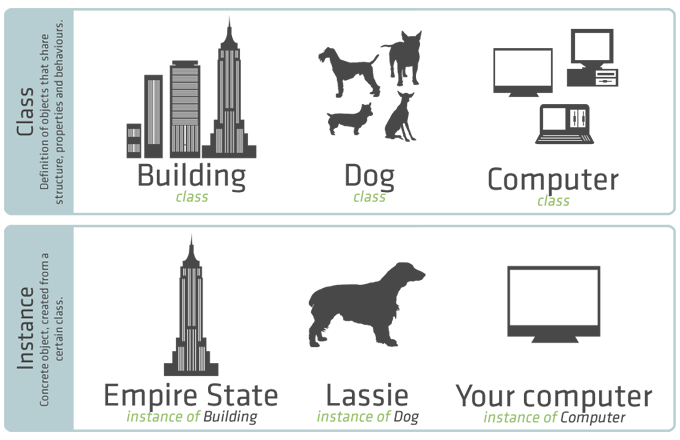
\includegraphics[width=0.8\linewidth]{figures/classes_instances.png}
  \caption{Graphical representation of a class instance.}
  \label{fig:classes}
\end{figure}

To see how classes can be defined let's try to code one representing a person:
\begin{ipythonnon}
from datetime import date        

class Person:
\end{ipythonnon}

First of all, if needed, we have to import the necessary modules, in this case the \texttt{datetime} module is used to manage the person age.
Then the \texttt{class} keyword followed by the class name is used to start the actual definition.

\subsubsection{The Constructor Method}\label{the-constructor-method}

After declaring the class name, the constructor method must be defined. In \texttt{python}, this is denoted by \texttt{\_\_init\_\_()} regardless the class name. The \texttt{\_\_init\_\_} method, as every other method in a class, takes \texttt{self} as the first argument, and then any number of parameters as desired by the programmer. The \emph{constructor} allows to specify the initial state of a class by setting its attribute values. For this example that describes a person, the programmer wants to know its name, the birthday and a job (this last one won't be initialize by the constructor though).

The \texttt{self} parameter is used to create class attributes. Variables whose name starts with \texttt{self.} have \emph{class scope}, which means are available within each class method. To use the parameters and associate them with a particular instance of the class, within the \texttt{\_\_init\_\_} method, create variables for each argument like this: \texttt{self.variableName\ =\ param}.

\begin{ipythonnon}
from datetime import date

# this is the class definition
# usually classes use camel naming convention
class Person:
    # the special method __init__ allows to instantiate a class
    # with an initial dataset
    def __init__(self, name, birthday):
        self.name = name
        self.birthday = birthday
        self.occupation = None # this attribute not set at instantiation
\end{ipythonnon}

Now that we have a class definition that represents a generic person we can specialized it to some real person.

\begin{ipythonnon}
me = Person("Matteo", date(1974, 10, 20))
print (type(me))
\end{ipythonnon}
\begin{ioutput}
<class '\_\_main\_\_.Person'>
\end{ioutput}

When we instantiate a class, \texttt{python} first calls the \texttt{\_\_init\_\_} method and initializes the attributes with the parameter we are passing.

\subsubsection{Class Methods}

We haven't yet defined any "person behavior", so let's add a couple of methods to our class: one computing the person's age and the other setting its primary occupation.

\begin{ipythonnon}
class Person:
    def __init__(self, name, birthday):
        self.name = name
        self.birthday = birthday
        self.employment = None

    # this is a normal method and will work on some class attribute
    def age(self, d=date.today()):
        age = (d - self.birthday).days/365
        print (f"{self.name} is {age:.0f} years old")

    def mainOccupation(self, occupation):
        self.employment = occupation
        print (f"{self.name}'s main occupation is: {self.employment}")
\end{ipythonnon}

To access class attributes and methods the dot (\texttt{.}) operator has to be used. 

\begin{ipythonnon}
print (me.name)
\end{ipythonnon}
\begin{ioutput}
'Matteo'
\end{ioutput}
        
\begin{ipythonnon}
me.age(date.today())
\end{ipythonnon}
\begin{ioutput}
Matteo is 46 years old
\end{ioutput}

\subsection{Inheritance and Overriding Methods}
\label{inheritance-and-overriding-methods}

Inheritance is basically the idea that different classes can have similar components, and in order to avoid repeating code, it is used to link parent to descendant classes. Inheritance allows the classes to share information relevant to multiple parts of the code.

For example, in a fantasy story, there are \emph{heroes} and \emph{monsters} but both of them are \emph{characters}. Similarly \emph{dragons} and \emph{orcs} are \emph{monsters}. Though they are different kind of monsters, they share some characteristics: they both have a color, a size and enemies. Orcs might have characteristics that dragons do not; for example which kind of weapon the orc carries (Fig.~\ref{fig:inheritance}). 

\begin{figure}[h]
  \centering
  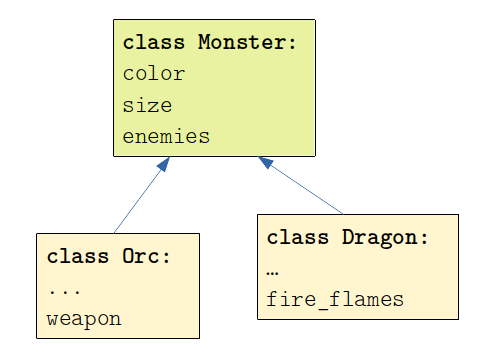
\includegraphics[width=0.5\textwidth]{figures/inheritance.png}
  \caption{Example of inheritance: both \texttt{Dragon} and \texttt{Orc} inherits from \texttt{Monster}, but both add additional attributes that qualify better each "monster features".}
  \label{fig:inheritance}
\end{figure}

Inheritance allows code to be reused and reduces the complexity of a program. The derived classes (descendants) override or extend the functionalities of the base classes (ancestors). To see how it works in more detail two derived class will be implemented from \texttt{Person}: \texttt{Adult} and \texttt{Child}.

\begin{ipythonnon}
class Adult(Person):
    def __init__(self, name, birthday, drv_license_id):
        Person.__init__(self, name, birthday) # this is a special syntax
        self.drv_license_id = drv_license_id

class Child(Person):
    def mainOccupation(self):
        self.employment = "schoolchild"
        print (f"{self.name} is a {self.employment}")
\end{ipythonnon}

Inheritance is specified in parenthesis after the class name. \texttt{Child} still inherits from \texttt{Person} and modifies it by setting the only occupation allowed for a child, overriding the \texttt{mainOccupation} method. \texttt{Adult} class inherits from \texttt{Person} too but extends it adding a new attribute, i.e. the driving license id. 

\begin{ipythonnon}
pippo = Adult("Goofy", date(1936, 1, 1), "A1234")
qui = Child("Huey", date(2014, 10, 9))
\end{ipythonnon}

Behind the scenes, when instantiating a \texttt{Child} class, the constructor of \texttt{Person} is called and the attributes, \texttt{name} and \texttt{birthday} are still initialized.  

For the \texttt{Adult} class things are a little bit different because a new attribute has been added, so we need to code its own constructor where we first call explicitly the \texttt{Person}'s constructor (\texttt{Person.\_\_init\_\_(self, \ldots)} and then we initialize the new attribute.

\begin{ipythonnon}
pippo.age()
pippo.mainOccupation("Comic's character")
\end{ipythonnon}
\begin{ioutput}
Goofy is 85 years old
Goofy's main occupation is: Comic's character
\end{ioutput}

\begin{ipythonnon}
qui.age()
qui.mainOccupation()
\end{ipythonnon}
\begin{ioutput}
Huey is 6 years old
Huey is a schoolchild
\end{ioutput}

\section*{Exercises}
\cprotEnv\begin{question}
Take the code for the Black-Scholes formula from exercise~\ref{ex:BS1} and wrap it in a function. Then, use this function to calculate the prices of calls with various strikes, using the following input data.

\begin{ipython}
s = 800 
# strikes expressed as % of spot price
moneyness = [0.5, 0.75, 0.825, 1.0, 1.125, 1.25, 1.5]
vol = 0.3
ttm = 0.75
r = 0.005
\end{ipython}

The output should be a dictionary mapping strikes to call prices.
\end{question}

\cprotEnv\begin{solution}
\begin{ipython}
from math import log, exp, sqrt
from scipy.stats import norm

def d1(St, K, r, vol, ttm):
    num = log(St/K) + (r + 0.5*pow(vol, 2)) * ttm
    den = vol * sqrt(ttm)
    return num/den

def d2(St, K, r, vol, ttm):
    return d1(St, K, r, vol, ttm) - vol*sqrt(ttm)

def call(St, K, r, vol, ttm):
    return St * norm.cdf(d1(St, K, r, vol, ttm)) - K * exp(-r*ttm)*norm.cdf(d2(St, K, r, vol, ttm))

s = 800
# strikes expressed as % of spot price
moneyness = [0.5, 0.75, 0.825, 1.0, 1.125, 1.25, 1.5]
vol = 0.3
ttm = 0.75
r = 0.005

result = {}
for m in moneyness:
    result[s*m] = call(s, m*s, r, vol, ttm)
print(result)

{400.0: 401.66074527896365,
  600.0: 213.9883852521275,
  660.0: 166.85957363897393,
  800.0: 84.03697017660357,
  900.0: 47.61880394696229,
  1000.0: 25.632722952585738,
  1200.0: 6.655275227771156}
\end{ipython}
\end{solution}

\cprotEnv\begin{question}
Write two classes, \texttt{Circle} and \texttt{Rectangle} that given the radius and height, width respectively allow to compute area and perimeter of the two shapes. Test them with the following:

\begin{ipython}
a_circle = Circle(5)
print("My circle has an area of {} m2".format(a_circle.area()))

a_rectangle = Rectangle(3, 6)
print ("My rectangle has a perimeter of {} m and an area of {} m2".format(a_rectangle.perimeter(), a_rectangle.area())}
\end{ipython}
\end{question}

\cprotEnv\begin{solution}
\begin{ipython}
from math import pi

class Circle:
    def __init__(self, radius):
        self.radius = radius

    def area(self):
        return pi*self.radius**2

class Rectangle:
    def __init__(self, width, height):
        self.height = height
        self.width = width

    def area(self):
        return self.width*self.height

    def perimeter(self):
        return self.width*2 + self.height*2

circle = Circle(5)
print ("My circle area is {:.1f} m**2".format(circle.area()))

rect = Rectangle(3, 6)
print ("My rect area is {:.1f} m**2 and the perimeter is {} m".format(rect.area(), rect.perimeter()))

My circle area is 78.5 m**2
My rect area is 18.0 m**2 and the perimeter is 18 m
\end{ipython}
\end{solution}

\cprotEnv\begin{question}
Define a class \texttt{Songs}, its \texttt{\_\_init\_\_} should take as input a dictionary (\texttt{lyrics} that contains lyrics line by line). Define a method, \texttt{sing\_me\_a\_song} that prints each element of the lyrics in his own line. Also test it with the following input.

\begin{ipython}
lyrics = {"Wonderwall":["Today is gonna be the day",
	                    "That they're gonna throw it back to you",
	                    "By now you should've somehow", "..."],
	      "Wish you were here": ["So, so you think you can tell",
                                 "Heaven from hell",
	                             "Blue skies from pain", "..."]}
\end{ipython}
\end{question}

\cprotEnv\begin{solution}
\begin{ipython}
class Songs:
    def __init__(self, lyrics):
        self.lyrics = lyrics

    def sing_me_a_song(self, title):
        song = self.lyrics[title]
        print ("Title: {}".format(title))
        print ("********************")
        for line in song:
            print (line)

lyrics = {"Wonderwall":["Today is gonna be the day",	
	                    "That they're gonna throw it back to you",
	                    "By now you should've somehow", "..."],
	      "Wish you were here": ["So, so you think you can tell",
                        "Heaven from hell",
                        "Blue skies from pain", "..."]}

songs = Songs(lyrics)
songs.sing_me_a_song("Wonderwall")

Title: Wonderwall
********************
Today is gonna be the day
That they're gonna throw it back to you
By now you should've somehow
...
\end{ipython}
\end{solution}

\begin{question}
Define a Point2D class that represent a point in a plane. Its \texttt{\_\_init\_\_} method should accept the point coordinates \texttt{x} and \texttt{y}. Write a method \texttt{distanceTo} that compute the distance of the point to another passed as input. Test the class by printing the distance of the point \(P=(4, 5)\) to the origin \(P=(0,0)\) and to \(P=(3,4)\).

\noindent\textbf{Hint:} in the Cartesian plane the distance between two points is: $\sqrt{(x_1 - x_2)^2 + (y_1 - y_2)^2}$.
\end{question}

\cprotEnv\begin{solution}
\begin{ipython}
from math import sqrt

class Point2D:
    def __init__(self, x, y):
        self.x = x
        self.y = y

    def distanceTo(self, x, y):
        dist = sqrt((self.x-x)**2 + (self.y - y)**2)
        return dist

    def distanceTo_v2(self, p):
        dist = sqrt((self.x-p[0])**2 + (self.y - p[1])**2)
        return dist

    def distanceTo_v3(self, p):
        dist = sqrt((self.x-p.x)**2 + (self.y - p.y)**2)
        return dist

point = Point2D(4, 5)
p0 = (0, 0)
point0 = Point2D(0, 0)
print ("distance to p0: {:.2f}".format(point.distanceTo(p0[0], p0[1])))
print ("distance_v2 to p0: {:.2f}".format(point.distanceTo_v2(p0)))
print ("distance_v3 to p0: {:.2f}".format(point.distanceTo_v3(point0)))
p1 = (3, 4)
point1 = Point2D(3, 4)
print ("distance to p1: {:.2f}".format(point.distanceTo(p1[0], p1[1])))
print ("distance_v2 to p1: {:.2f}".format(point.distanceTo_v2(p1)))
print ("distance_v3 to p1: {:.2f}".format(point.distanceTo_v3(point1)))

distance to p0: 6.40
distance\_v2 to p0: 6.40
distance\_v3 to p0: 6.40
distance to p1: 1.41
distance\_v2 to p1: 1.41
distance\_v3 to p1: 1.41
\end{ipython}
\end{solution}

\cprotEnv\begin{question}
Write a class \texttt{Student} which inherits from the class \texttt{Person} defined in Chapter Object Oriented Programming in Python. This new class should have two new attributes: \texttt{grade} which keeps the type of school and \texttt{votes} a dictionary which will record the student's votes and the corresponding course. Then add two methods, one to add votes and another to compute the average vote.Instantiate a "student" add some votes and show how good it has been.

\noindent\textbf{Hint:} this is the \texttt{Person} class already developed.

\begin{ipython}
class Person:
    def __init__(self, name, birthday):
        self.name = name
        self.birthday = birthday
        self.employment = None

    def age(self, d=date.today()):
        age = (d - self.birthday).days/365
        print ("{} is {:.0f} years old".format(self.name, age))

    def mainOccupation(self, occupation):
        self.employment = occupation
        print ("{}'s main occupation is: {}".format(self.name, self.employment))
\end{ipython}
\end{question}

\cprotEnv\begin{solution}
\begin{ipython}
class Student(Person):
    def __init__(self, name, birthday, school):
        Person.__init__(self, name, birthday)
        self.grade = school
        self.votes = {}

    def addVote(self, subject, vote):
        self.votes[subject] = vote

    def average(self):
        print ("List of votes")
        print ("-------------")
        for k, v in self.votes.items():
            print ("{}: {}".format(k, v))
        avg = sum(self.votes.values())/len(self.votes)
        print ("-------------")
        print ("Avg: {:.1f}".format(avg))

student = Student("Mario", date(1980, 5, 6), "Liceo Scientifico G. Galilei")
student.addVote("Calculus", 8)
student.addVote("Literature", 5.5)
student.addVote("Latin", 6.5)
student.average()

List of votes
-------------
Calculus: 8
Literature: 5.5
Latin: 6.5
-------------
Avg: 6.7
\end{ipython}
\end{solution}


\chapter{Data Manipulation and Its Representation}
\label{sec:datamanip}

In this Chapter a closer look two a couple more of modules is given. These modules result to be very useful in managing financial data and to report results of our analysis.

\section{Getting Data}\label{getting-data}

The first step of any analysis is usually the one that involves selection and manipulation of data we want to process. Data sources can be various (e.g. website, figures, twitter messages, CSV or Excel files\ldots) and partially reflect its nature which can range from \emph{unstructured} data (without any inherent structure, e.g. social media data) to completely \emph{structured} data (where the data model is defined and usually there is no error associated, e.g. stock trading data).

Various modules are available in \texttt{python} to gather financial data for our studies: \texttt{quandl}~\cite{bib:quandl}, \texttt{yfinance}~\cite{bib:yfinance},\texttt{ffn}~\cite{bib:ffn}\ldots

Below a simple example using \texttt{yfinance}, that retrieves the closing prices of few securities. The same job with \texttt{quandl} is just a little bit more complicated since it involves the request for a token, but it just takes few minutes more.  

\begin{ipython}
import yfinance as yf

tickers = ['SPY','TLT','MSFT']
	
proxy = yf.Tickers(tickers)

data = proxy.history(start="2021-01-01", end="2021-08-10")
print (data.head())
\end{ipython}
\begin{ioutput}
[*********************100%***********************]  3 of 3 completed
                 Close                         Dividends            \
                  MSFT         SPY         TLT      MSFT  SPY  TLT   
Date                                                                 
2020-12-31  221.397675  371.444244  156.292892       0.0  0.0  0.0   
2021-01-04  216.689423  366.387390  156.104645       0.0  0.0  0.0   
2021-01-05  216.898438  368.910828  154.945297       0.0  0.0  0.0   
2021-01-06  211.274414  371.116394  151.764557       0.0  0.0  0.0   
2021-01-07  217.286652  376.630249  150.426834       0.0  0.0  0.0   

                  High                                 Low  ...              \
                  MSFT         SPY         TLT        MSFT  ...         TLT   
Date                                                        ...               
2020-12-31  221.975010  372.219162  156.639710  218.670263  ...  156.015445   
2021-01-04  221.975014  373.004005  156.738813  213.822655  ...  155.113756   
2021-01-05  217.515598  370.073219  155.520015  214.708553  ...  154.241775   
2021-01-06  215.494931  374.524071  152.448273  210.965841  ...  150.902473   
2021-01-07  218.331828  377.425025  150.783555  212.727716  ...  149.881842   

                  Open                                 Stock Splits    Volume  \
MSFT               SPY         TLT                     MSFT SPY TLT      MSFT   
Date                                                                            
2020-12-31  220.680983  369.357919  156.025363            0   0   0  20942100   
2021-01-04  221.507173  372.864902  155.242576            0   0   0  37130100   
2021-01-05  216.261380  365.701890  155.520015            0   0   0  23823000   
2021-01-06  211.194780  367.301414  152.418547            0   0   0  35930700   
2021-01-07  213.056186  373.649793  150.407012            0   0   0  27694500   


                  SPY       TLT  
Date                             
2020-12-31   78520700   7742100  
2021-01-04  110210800  13152900  
2021-01-05   66426200  10458100  
2021-01-06  107997700  22827300  
2021-01-07   68766800  14651900  

[5 rows x 21 columns]
\end{ioutput}

The \texttt{history} method returns a dataframe (a particular data structure that will be described later in this Chapter) with a lot of information concerning the selected stocks like open and close prices, dividends, volume etc\ldots
eside the \texttt{start} and \texttt{end} parameters which define the range in which to retrieve data another useful one is \texttt{interval} which specifies its granularity. It can take the following values: 1m, 2m, 5m, 15m, 30m, 60m, 90m, 1h, 1d, 5d, 1wk, 1mo, 3mo. However it is important to note that the 1m data is only retrievable for the last 7 days, and anything intraday (interval <1d) only for the last 60 days.

Note that the table contains also dates in which may be dividends (in this case there are none so the rows are NaN).
  
In the following example we are going to download the monthly historical series of the closing price of our stocks.

\begin{ipython}
data = proxy.history(start="2021-01-01", end="2021-08-10", interval='1mo')['Close']
print (data.head())
\end{ipython}
\begin{ioutput}
[*********************100%***********************]  3 of 3 completed
                  MSFT         SPY         TLT
Date                                          
2021-01-01  230.893845  367.659088  150.615112
2021-02-01  231.311905  377.882019  141.816010
2021-02-17         NaN         NaN         NaN
2021-03-01  235.226837  393.747986  134.371506
2021-03-19         NaN         NaN         NaN
\end{ioutput}

When dealing with just one ticker it is possible to display many financial information related to the company by using \texttt{info}. It will show all the information regarding the company including its Sector, No. of Employees, Business Summary, etc\ldots

\begin{ipython}
proxy = yf.Ticker('MSFT')

print (proxy.info)
\end{ipython}
\begin{ioutput}
\{'zip': '98052-6399', 'sector': 'Technology', 'fullTimeEmployees': 181000, 
'longBusinessSummary': 'Microsoft Corporation develops, ...'companyOfficers': [], 
'website': 'http://www.microsoft.com', 'maxAge': 1, 'address1': 'One Microsoft Way', 
'industry': 'Software-Infrastructure', 'ebitdaMargins': 0.48080003, ....\}
\end{ioutput}

Financial data analysts sometimes require details about dividends and splits the company has given to its shareholders. With the \texttt{actions} method, can be downloaded.

\begin{ipython}
print (proxy.actions)
\end{ipython}
\begin{ioutput}
            Dividends  Stock Splits
Date                               
1987-09-21       0.00           2.0
1990-04-16       0.00           2.0
1991-06-27       0.00           1.5
1992-06-15       0.00           1.5
1994-05-23       0.00           2.0
...               ...           ...
2020-05-20       0.51           0.0
2020-08-19       0.51           0.0
2020-11-18       0.56           0.0
2021-02-17       0.56           0.0
2021-05-19       0.56           0.0

[79 rows x 2 columns]
\end{ioutput}

Other than the \texttt{actions} function we can use \texttt{dividends} and \texttt{splits} functions separately to view them individually.

To know the sustainability of the stock there is a predefined function named \texttt{sustainability} which can be used to display data about that.

\begin{ipython}
print (proxy.sustainability)
\end{ipython}
\begin{ioutput}
                                     Value
2021-5                                    
palmOil                              False
controversialWeapons                 False
gambling                             False
socialScore                           9.37
nuclear                              False
furLeather                           False
alcoholic                            False
gmo                                  False
catholic                             False
socialPercentile                      None
peerCount                              103
governanceScore                       4.83
environmentPercentile                 None
animalTesting                        False
tobacco                              False
totalEsg                             14.63
highestControversy                       3
esgPerformance                  UNDER_PERF
coal                                 False
pesticides                           False
adult                                False
percentile                            7.59
peerGroup              Software & Services
smallArms                            False
environmentScore                      0.42
governancePercentile                  None
militaryContract                     False
\end{ioutput}

Recommendations for buying or selling a company’s stock is provided by different financial firms. In order to analyze the stock price, we must know what these firms recommend. To analyze the recommendations the \texttt{recommendations} method can be used.

\begin{ipython}
print (proxy.recommendations)
\end{ipython}
\begin{ioutput}
                               Firm       To Grade From Grade Action
Date                                                                
2012-03-16 08:19:00  Argus Research            Buy                up
2012-03-19 14:00:00  Hilliard Lyons  Long-Term Buy              main
2012-03-22 07:03:00  Morgan Stanley     Overweight              main
2012-04-03 11:53:00             UBS            Buy              main
2012-04-20 06:18:00   Deutsche Bank            Buy              main
...                             ...            ...        ...    ...
2021-07-28 14:47:46        Barclays     Overweight              main
2021-07-28 14:49:16       Citigroup            Buy              main
2021-07-28 14:51:12          Mizuho            Buy              main
2021-07-28 14:54:54   Credit Suisse     Outperform              main
2021-07-29 10:53:54       JP Morgan     Overweight              main
\end{ioutput}

\texttt{calendar} function can be used to know about the earnings and revenue of the company.

\begin{ipython}
print (proxy.calendar)
\end{ipython}
\begin{ioutput}
                                    0                    1
Earnings Date     2021-10-25 10:59:00  2021-10-29 12:00:00
Earnings Average                 1.90                 1.90
Earnings Low                     1.64                 1.64
Earnings High                    2.03                 2.03
Revenue Average           44102900000          44102900000
Revenue Low               40850000000          40850000000
Revenue High              44914700000          44914700000
\end{ioutput}

For every company listed on the stock market, there is a unique ISIN (International Securities Identification Number) number, ut can be found using \texttt{isin} method.

\begin{ipython}
print (proxy.isin)
\end{ipython}
\begin{ioutput}
US5949181045
\end{ioutput}

Concerning option trading on a particular stock, the module allows to get expiry dates with \texttt{options} method.

\begin{ipython}
print (proxy.options)
\end{ipython}
\begin{ioutput}
('2021-08-13', '2021-08-20', '2021-08-27', '2021-09-03', '2021-09-10', 
 '2021-09-17', '2021-09-24', '2021-10-15', '2021-11-19', '2021-12-17', 
 '2022-01-21', '2022-03-18', '2022-06-17', '2022-09-16', '2023-01-20', 
 '2023-03-17', '2023-06-16')
\end{ioutput}

To get associated calls data:
\begin{ipython}
opt = proxy.option_chain(date='2021-08-13')
print (opt.calls)
\end{ipython}
\begin{ioutput}
         contractSymbol       lastTradeDate  strike  lastPrice  bid  ask  \
0   MSFT210813C00180000 2021-08-09 14:48:40   180.0     109.05  0.0  0.0   
1   MSFT210813C00185000 2021-08-09 13:35:15   185.0     105.45  0.0  0.0   
2   MSFT210813C00190000 2021-08-03 15:04:10   190.0      95.10  0.0  0.0   
3   MSFT210813C00195000 2021-08-03 14:35:40   195.0      89.60  0.0  0.0   
4   MSFT210813C00200000 2021-08-09 13:37:35   200.0      89.26  0.0  0.0   
5   MSFT210813C00205000 2021-08-03 14:11:33   205.0      79.85  0.0  0.0   
...

    change  percentChange   volume  openInterest  impliedVolatility  \
0      0.0            0.0      5.0             5           0.000010   
1      0.0            0.0      3.0             0           0.000010   
2      0.0            0.0      NaN             4           0.000010   
3      0.0            0.0      1.0            10           0.000010   
4      0.0            0.0      1.0             8           0.000010   
5      0.0            0.0      1.0             0           0.000010   
...

    inTheMoney contractSize currency  
0         True      REGULAR      USD  
1         True      REGULAR      USD  
2         True      REGULAR      USD  
3         True      REGULAR      USD  
4         True      REGULAR      USD  
5         True      REGULAR      USD  
\end{ioutput}

These are the main features of \texttt{yfinance} which can be used for stock data analysis. A more detailed guide can be found \href{https://algotrading101.com/learn/yfinance-guide/}{\emph{here}}.

\section{Manipulating Data}
Before start processing data, it is neccessary to store the information in a suitable data structure. \texttt{python} provides a very useful module, called \texttt{pandas}~\cite{pandas}, which allows to collect and save data in \emph{dataframe} objects that can be later on manipulated for analysis purposes.

Looking at \texttt{pandas} manual, dataframes are defined as "multi-dimensional, size-mutable, potentially heterogeneous, tabular data structure with labeled axes (rows and columns)", in much simpler words it is a table whose structure can be modified.
It contains multiple methods for convenient data filtering and in addition has a lot of utilities to load and save data pretty easily.

I like to think them as a tabulated board where all results, scores, tests and conditions are annotated and passed between the different analysis stages. Each stage uses previous data and adds data to the board and at the end of the simulation, the dataframe contains all the information to evaluate the result.


Dataframes can be created by:
\begin{itemize}
\tightlist
\item importing data from file (\href{https://github.com/matteosan1/finance_course/blob/develop/libro/input_files/sample.xlsx?raw=true}{sample.xlsx}, \href{https://raw.githubusercontent.com/matteosan1/finance_course/develop/libro/input_files/sample.csv}{sample.csv});
\item creating by hand data and then filling the dataframe.
\end{itemize}

\begin{ipython}
import pandas as pd

# reading from file
df1 = pd.read_excel('sample.xlsx') # Excel file
df2 = pd.read_csv('sample.csv') # Comma Separated file
print (df1.head(11)) # show just few rows at the beginning
\end{ipython}
\begin{ioutput}
         Date      Price     Volume
0  2020-05-18  78.739998  135178400
1  2020-05-19  78.285004  101729600
2  2020-05-20  79.807503  111504800
3  2020-05-21  79.212502  102688800
4  2020-05-22  79.722504   81803200
5  2020-05-26  79.182503  125522000
6  2020-05-27  79.527496  112945200
7  2020-05-28  79.562500  133560800
8  2020-05-29  79.485001  153532400
9  2020-06-01  80.462502   80791200
10 2020-06-02  80.834999   87642800
\end{ioutput}

\begin{ipython}
# creating some data in a dictionary
d = {"Name":["Elisa", "Roberto", "Ciccio", "Topolino", "Gigi"],
	 "Age":[1, 27, 25, 24, 31],
	 "Points":[100, 120, 95, 1300, 101]}

# filling the dataframe
df = pd.DataFrame(d)
print (df.head())
\end{ipython}
\begin{ioutput}
       Name  Age     Points
0     Elisa    1        100
1   Roberto   27        120
2    Ciccio   25         95
3  Topolino   24       1300
4      Gigi   31        101
\end{ioutput}

It is possible to perform a large number of operations on dataframes, for example add a column as a result of an operation on other columns. 
Looking back at dataframe \texttt{df1} it is possible to add a column with the daily variation of the price.

\begin{ipython}
import numpy as np

# first let's add an empty column
df1['Variation'] = np.nan # nan stands for not a number

# loop on the Price column, compute the variation and fill the column
# len returns the number of rows of a dataframe
for i in range(1, len(df1)):
    # select the ith row and fill "Variation"
    # loc takes as inputs row and colum-name
    df1.loc[i, "Variation"] = (df1.loc[i, "Price"] - df1.loc[i-1, "Price"]) /
        df1.loc[i-1, "Price"]
print (df1.head())
\end{ipython}
\begin{ioutput}
        Date      Price     Volume  Variation
0 2020-05-18  78.739998  135178400        NaN
1 2020-05-19  78.285004  101729600  -0.005778
2 2020-05-20  79.807503  111504800   0.019448
3 2020-05-21  79.212502  102688800  -0.007455
4 2020-05-22  79.722504   81803200   0.006438	
\end{ioutput}
\noindent
However there are simpler ways to achieve the same result. Indeed writing a formula for a dataframe column implies to compute the result for each row. So the first alternative doesn't require a for loop to cycle among the rows. The \texttt{shift} function consider a row shifted by the specified amount with respect to the "current" one.

The second option relies instead on a built in method that exactly computes the percentage variation between a row and the previous.

\begin{ipython}
# single line option
df1['Variation'] = data['Price'].pct_change()

# second single line option
data['Variation'] =  (data['Close']-data['Close'].shift(1))/data['Close'].shift(1)
\end{ipython}

Of course the first "variation" value is NaN since there is no previous price to compare with. NaN, short for \emph{not a number}, represents the \texttt{null} value, it is the value that is given to missing fields in a row. 

\subsection{Manage Data}\label{manage-data}

Once we have created our dataframe we may want to preliminary process data to perform very common operations like:

\begin{itemize}
	\tightlist
\item remove unwanted observations or outliers;
\item handle missing data;
\item filter, sort and clean data.
\end{itemize}

\subsection{Unwanted observations and outliers}

\subsubsection{Duplicates}

It may happen that data has duplicates (e.g. those can arise when combining two datasets), or the dataset contains irrelevant fields for the specific study we are carrying on. To find and remove duplicates \texttt{pandas} has convenient methods:

\begin{ipython}
# find duplicates based on all columns
# and show just the first 15 results
#print (df1.duplicated()[:15])

# find duplicates based on'Price'
# and show just the first 15 results
print (df1.duplicated(subset=['Price'])[:15] )
\end{ipython}
\begin{ioutput}
0     False
1     False
2     False
3     False
4      True
5     False
6     False
7     False
8     False
9     False
10    False
11     True
12     True
13    False
14    False
dtype: bool
\end{ioutput}

\begin{ipython}
print ("Initial number of rows: {}".format(len(df1)))

# remove duplicates
# where the second argument can be `first` , `last`
# or `False` (consider all of the same values as duplicates).

df1 = df1.drop_duplicates(subset='Price', keep='first')
print ("Number of columns after drop: {}".format(len(df1)))
\end{ipython}
\begin{ioutput}
Initial number of rows: 254
Number of columns after drop: 248
\end{ioutput}

If we would like to drop irrelevant columns for our analysis it is enough to:

\begin{ipython}
df2 = df2.drop(columns=['Volume'])
print (df2.head())
\end{ipython}
\begin{ioutput}
         Date      Price
0  18/05/2020  78.739998
1  19/05/2020  78.285004
2  20/05/2020  79.807503
3  21/05/2020  79.212502
4  22/05/2020  79.722504
\end{ioutput}
        
If instead we just want to remove few rows we can select them by index:

\begin{ipython}
# we remove row 0th and 2nd
# axis=0 means use the index column
df2 = df2.drop([0, 2], axis=0)
print (df2.head())
\end{ipython}
\begin{ioutput}
         Date      Price
1  19/05/2020  78.285004
3  21/05/2020  79.212502
4  22/05/2020  79.722504
5  26/05/2020  79.182503
6  27/05/2020  79.527496
\end{ioutput}
        
Changing the column that act as index we can select the rows also by other attributes:

\begin{ipython}
# tell pandas to use Date as index column
df2 = df2.set_index('Date')

# select row to remove by date at this point
df2 = df2.drop(["2000-07-31"], axis=0)
print (df2.head())
\end{ipython}
\begin{ioutput}
                Price
Date                 
21/05/2020  79.212502
22/05/2020  79.722504
26/05/2020  79.182503
27/05/2020  79.527496
28/05/2020  79.562500
\end{ioutput}
        
\subsubsection{Outliers}\label{outliers}

An outlier is an observation that lies outside the overall pattern of a distribution. Common causes can be human, measurement or experimental errors. Outliers must be handled carefully and should be removed cautiously, \emph{outliers are innocent until proven guilty}. We may have removed the most interesting part of our dataset !

The core statistics about a particular column can be studied by the \texttt{describe()} method which returns the following information:
\begin{itemize}
	\tightlist
\item for numeric columns: the value count, mean, standard deviation, minimum, maximum and 25th, 50th and 75h quantiles for the data in a column;
\item for string columns: the number of unique entries, the most frequent occurring value (\emph{top}), and the number of times the top value occurs (\emph{freq}).
\end{itemize}

\begin{ipython}
print (df1.describe())
\end{ipython}
\begin{ioutput}
              Price        Volume   Variation
count    248.000000  2.430000e+02  247.000000
mean     163.747117  1.287922e+08    0.393586
std      748.572478  5.309638e+07    6.210597
min       78.285004  4.669130e+07   -0.990255
25%      110.274997  9.032360e+07   -0.008365
50%      120.109996  1.129452e+08    0.001749
75%      128.132504  1.536495e+08    0.016365
max    11902.000000  3.743368e+08   97.599951
\end{ioutput}
        
Looking at mean and std and comparing it with min and max values we could find a range outside of which we may have outliers. For example 11902.0 is several standard deviation away the mean which may indicate that it is not a good value.

Another way to spot outliers is to plot column distributions and again \texttt{pandas} comes to help us:
\begin{ipython}
df1.hist("Variation", bins=np.arange(0, 100, 1))
\end{ipython}

\begin{figure}
	\centering
	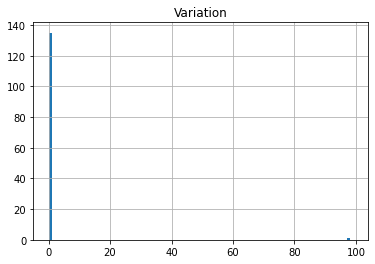
\includegraphics[width=0.7\linewidth]{figures/volume_plot}
\end{figure}

From the histograms it is clear how the value of 97.60, is far from general population. This doesn't mean it is necessarily wrong but it should make ring a bell in our head\ldots

To remove outliers from data we can either remove the entire rows or replace the suspicious values by a default one 
(e.g. 0, 1, a threshold value\ldots).

\textbf{Note}: missing data may be informative itself~!~When filling the gap with \emph{artificial data} (e.g. mean, median, std\ldots) having similar properties than real observation, the added value won't be scientifically valid, no matter how sophisticated your filling method is.

\begin{ipython}
import numpy as np

df2 = df2.replace(11902, 500) # replace 11902 with 500
df2 = df2.replace(11902, np.nan) # replace 11902 with NaN
df2 = df2.mask(df1 >= 150, 5) # replace every element >=600 with 5
\end{ipython}

\subsection{Handle Missing Data}\label{handle-missing-data}

Usually when importing data with \texttt{pandas} we may have some NaN values. Like for the outliers we can use the \texttt{replace} or \texttt{mask} methods to remove the NaNs. In case the whole row as NaN it may be wise to drop it entirely.

Additionally we can use \texttt{dropna()} which remove all the NaN in the dataframe at once.

\begin{ipython}
df1 = df1.dropna()
print ("Number of rows after dropping NaN: {}".format(len(df1)))
\end{ipython}
\begin{ioutput}
Number of rows after dropping NaN: 242
\end{ioutput}

\subsection{Filter, Sort and Clean Data}
\label{filter-sort-and-clean-data}

\subsubsection{Filtering}\label{filtering}

When we work with huge datasets we may reach computational limits (e.g. insufficient memory, CPU performance, too slow processing time\ldots) and in those cases it can be helpful to filter data by attributes for example splitting by time or some other property.

Assuming to have the following table and putting back the volume column

\begin{ipython}
# df.iloc[row, col]
# NOTE: iloc takes row and column index (two numbers)
# loc instead takes row index and column name

print (df1.iloc[1, 2]) # returns 62 the volume associated with the row
\end{ipython}
\begin{ioutput}
111504800.0
\end{ioutput}

\begin{ipython}
#df.iloc[row1:row2, col1:col2]
# this is called slicing, remember ?

print (df1.iloc[0:2, 2:3]) # returns rows 0 and 1 of column 2
\end{ipython}
\begin{ioutput}
        Volume
1  101729600.0
2  111504800.0
\end{ioutput}

\begin{ipython}
subset = df1.iloc[:, 1] # select column 1
subset = df1.iloc[2, :] # select row 2
subset = df1.iloc[0:2, :] # select 2 rows
subset = df1.iloc[:2, :] # this is equivalent to before
\end{ipython}

A more advanced way of filtering is the following (it apply a selection on the values). The notation is a bit awkward but very useful:

\begin{ipython}
import datetime

# colon means all the rows
subset = df1[df1.iloc[:, 0] < datetime.datetime(2020, 8, 15)]
print (subset)
\end{ipython}
\begin{ioutput}
         Date       Price       Volume  Variation
1  2020-05-19   78.285004  101729600.0  -0.005778
2  2020-05-20   79.807503  111504800.0   0.019448
3  2020-05-21   79.212502  102688800.0  -0.007455
5  2020-05-22   79.722504   81803200.0   0.006438
6  2020-05-26   79.182503  125522000.0  -0.006774
..        ...         ...          ...        ...
61 2020-08-10  112.727501  212403600.0   0.014535
62 2020-08-11  109.375000  187902400.0  -0.029740
63 2020-08-12  113.010002  165598000.0   0.033234
64 2020-08-13  115.010002  210082000.0   0.017698
65 2020-08-14  114.907501  165565200.0  -0.000891

[61 rows x 4 columns]
\end{ioutput}

\subsubsection{Sorting}\label{sorting}

To sort data we can use \texttt{sort\_values()} method (it can be specified ascending, descending).

\begin{ipython}
# sort by price then by date in descending order
print (df2.sort_values(by=['Price', "Date"], ascending=False)[:10])
\end{ipython}
\begin{ioutput}
                 Price
Date                  
26/01/2021  143.160004
25/01/2021  142.919998
27/01/2021  142.059998
22/01/2021  139.070007
04/02/2021  137.389999
28/01/2021  137.089996
08/02/2021  136.910004
21/01/2021  136.869995
05/02/2021  136.759995
28/12/2020  136.690002
\end{ioutput}
        
\subsubsection{Cleaning or Regularizing}
\label{cleaning-or-regularizing}

As we will see when dealing with machine learning, often we need to regularize our data to improve the stability of a training. One typical situation is when we want to \emph{normalize} data, which means re-scale the values into a range of $[0, 1]$.

\begin{equation*}
\begin{gathered}
x = [1,43,65,23,4,57,87,45,45,23]\\
x_{new} = \cfrac{x - x_{min}}{x_{max} - x_{min}}\\
x_{new} = [0,0.48,0.74,0.25,0.03,0.65,1,0.51,0.51,0.25]
\end{gathered}
\end{equation*}

To apply such a transformation with \texttt{pandas} is very easy: 
\begin{ipython}
df1['Price'] = (df1['Price'] - df1['Price'].min()) \
    / (df1['Price'].max() - df1['Price'].min())
print (df1.head())
\end{ipython}
\begin{ioutput}
        Date     Price       Volume  Variation
1 2020-05-19  0.000000  101729600.0  -0.005778
2 2020-05-20  0.000129  111504800.0   0.019448
3 2020-05-21  0.000078  102688800.0  -0.007455
5 2020-05-22  0.000122   81803200.0   0.006438
6 2020-05-26  0.000076  125522000.0  -0.006774
\end{ioutput}
        
Another quite common transformation is called \emph{standardization}, essentially we re-scale data to have 0 mean and standard deviation of 1:

\begin{equation}
x_{new} = \cfrac{x-\mu}{\sigma}
\label{eq:standardization}
\end{equation}

Again it is straightforward to do it in \texttt{pandas}:

\begin{ipython}
df1.hist('Volume', bins=np.arange(180, 220, 1))

print (df1['Volume'].mean())
print (df1['Volume'].std())
\end{ipython}
\begin{ioutput}
128765806.61157025
53204829.93713034
\end{ioutput}

\begin{ipython}
df1['Volume'] = (df1['Volume'] - df1['Volume'].mean()) / df1['Volume'].std()
df1.hist('Volume', bins=np.arange(-5, 5, 0.1))

print (df1['Volume'].mean())
print (df1['Volume'].std())
\end{ipython}
\begin{ioutput}
-1.5598174726138563e-17
1.0
\end{ioutput}

Figure~\ref{fig:standardization} shows the comparison of the "volume" distribution before and after stadardization.

\begin{figure}[htb]
	\centering
	\subfloat[Original.]{%
		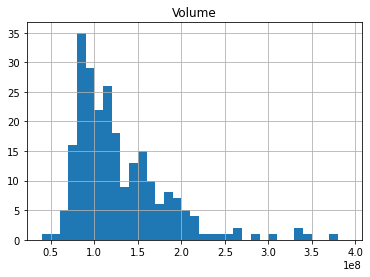
\includegraphics[width=0.45\textwidth]{figures/volume_plot_2}
	}
	\subfloat[Standardized according to Eq.~\ref{eq:standardization}.]{%
		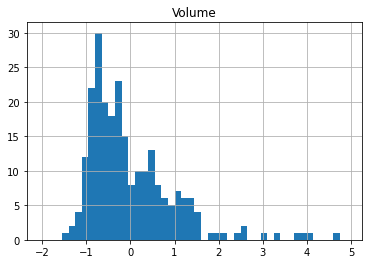
\includegraphics[width=0.45\textwidth]{figures/volume_plot_3}
	}
	\caption{Comparison between "volume" distributions.}
	\label{fig:standardization}
\end{figure}

\subsection{Operations on Data}
Using \texttt{pandas} all sorts of calculations between rows or columns can be made. Some example of that will be shown in the next Chapters, here just a simple application of Moving Average (MA) is described.

In finance, technical analysis is an analysis methodology for forecasting the direction of prices through the study of past market data, primarily price and volume. Technical analysts rely on a combination of technical indicators to study a stock and give insight about possible trading strategies. 

Consider for example a particular indicator called \emph{Bollinger Bands}. It is usually used to provide potential buy / sell signals and to define the prevailing high and low prices in a market to characterize the trading band of a financial instrument or commodity. You can think of Bollinger Bands as a volatility indicator. Bands consist of Moving Average lines, a upper band and lower band. The upper and lower bands are simply MA adding and subtracting standard deviation ($\sigma$), which is a sort of  measurement of volatility. 
\[
\begin{split}
\textrm{Upper Band} & = (\textrm{MA} + K\sigma)\\
\textrm{Lower Band} & = (\textrm{MA} − K\sigma)
\end{split}
\]

In the following example we are going to use a 20 day moving average and $K=2$. Imagine to have the historical series of AMZN stock closing prices. Bollinger Bands can be quickly and easily constructed as follows 

\begin{ipython}
import yfinance as yf
import pandas as pd
import matplotlib.pyplot as plt

proxy = yf.Ticker('AMZN')
df = proxy.history(start='2017-04-02', end='2018-05-02')['Close']

# calculate Moving Average with 20 days window
ma = df.rolling(window=20).mean()

# calculate the standard deviation
rstd = df.rolling(window=20).std()

df['upper'] = ma + 2 * rstd
df['lower'] = ma - 2 * rstd

ax = df.plot(title='AMZN Price and Bollinger Bands', figsize=(10,8))
ax.fill_between(df.index, df['lower'], df['upper'], color='#ADCCFF', alpha='0.4')
ax.set_xlabel('date')
ax.set_ylabel('Price Moving Average')
ax.set_xlim('2017-05-02', '2018-05-02')
ax.grid()
\end{ipython}

The resulting plot is shown in Fig.~\ref{fig:bollinger_bands} which can be interpreted by saying that approximately 90\% of prices lay between the two bands. Therefore the bands can be used to identify potential overbought or oversold conditions. If stock price breaks out the upper band, it could be an overbought condition (indication of short). Similarly, when it breaks out the lower band, it could be oversold condition (indication of long). 

\begin{figure}[htb]
	\centering
	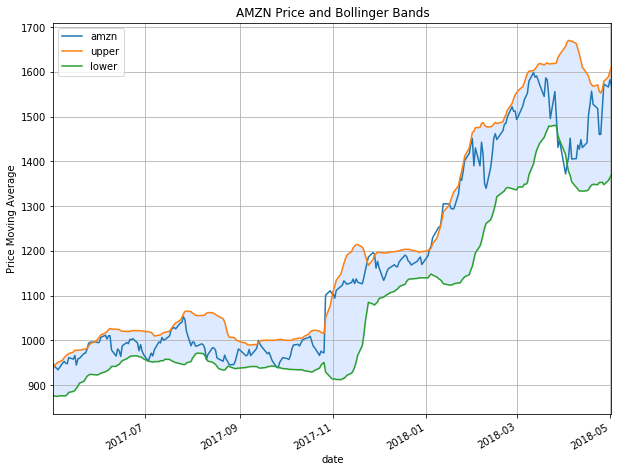
\includegraphics[width=0.7\textwidth]{figures/bollinger_bands}
	\caption{Bollinger Bands plot applied to AMZN historical prices.}
	\label{fig:bollinger_bands}
\end{figure}

\section{Plotting in \texttt{python}}\label{plotting-in-python}

As we have just seen \texttt{pandas} allows to quickly draw histograms of dataframe columns, but during an analysis we may want to plot distributions from \texttt{list} or objects not stored in a dataframe. Furthermore the simple although very useful interface doesn't grant full access to all plotting features that we need to produce nice and informative plots.

In order to do so we can use the \texttt{matplotlib} module which is specifically dedicated to plotting (\texttt{pandas} interface is based on the same module indeed). 

In the next Sections we will look briefly to its capabilities. For those interested a more detailed and comprehensive documentation can be found at~\cite{matplotlib}.

\subsection{Canvas}\label{canvas}

The first element we need to plot is a \emph{canvas}, the white rectangular space where we draw our data. \texttt{Matplotlib} provides a default canvas if no specific command is given (a 640x480 pixels space) but you can customize it by specifying many different parameters, the most common are:

\begin{itemize}
	\tightlist
	\item
	\texttt{figsize}: width, height in inches. If not provided, defaults to \([6.4, 4.8]\);
	\item
	\texttt{dpi}: resolution of the figure. If not provided, defaults to 100;
	\item
	\texttt{facecolor}: the background color. If not provided, defaults to \texttt{'white'}, or \texttt{'w'}.
\end{itemize}

In the following example we create a canvas (8 inches x 5 inches) with a resolution of 80 dots per inches (dpi) and a green background color.

\begin{ipython}
from matplotlib import pyplot as plt

fig = plt.figure(figsize=(8,5), dpi=80, facecolor='green')
\end{ipython}

Once we have a canvas we cannot even draw it unless we have some plot to show. So let's see the most commonly used types of plot.

\subsection{Chart Object}\label{chart-object}

Below a concise list of the main chart objects that are used when presenting financial data.

\subsubsection{Histograms}\label{histograms}

A histogram is an approximate representation of the distribution of numerical data. To construct a histogram, the first step is to \emph{bin} (or \emph{bucket}) the range of values (i.e. divide the entire range of values into a series of intervals) and then count how many values fall into each interval.

If the bins are of equal size, a rectangle is erected over the bin with height proportional to the frequency (i.e. the number of cases in each bin).
However, bins need not be of equal width; in that case, the erected rectangle is defined to have its area proportional to the frequency of cases in the bin. 
The vertical axis is then not the frequency but frequency density (i.e. the number of cases per unit of the variable on the horizontal axis).

To create a histogram with \texttt{matplotlib} it is enough to pass a list (or a \texttt{numpy.array}) with data to represent to the function \texttt{hist} and then call \texttt{show()} to actually draw the plot (I have used the previously defined canvas just to show the results), Fig.~\ref{fig:histo1}.

\begin{ipython}
y1 = [40.9, 47.7, 40.6, 43.0, 45.4, 42.3, 33.8, 49.6,
47.6, 52.3, 43.1, 36.5, 43.7, 52.4, 37.0, 42.4, 38.4, 39.9, 40.6, 35.7, 42.4,
38.3, 43.6, 38.5, 43.5, 42.9, 42.1, 39.8, 35.8, 44.1,
41.5, 42.6, 45.4, 38.6, 37.3, 37.8, 48.1, 44.8, 32.7, 40.3]

fig = plt.figure(figsize=(8,5), dpi=80, facecolor='green')
plt.hist(y1)
plt.show()
\end{ipython}

\begin{figure}[htb]
	\centering
	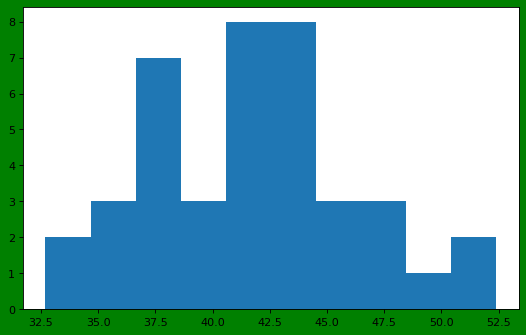
\includegraphics[width=0.7\textwidth]{figures/histo1}
	\caption{Example of histogram drawn on the previously defined canvas.}
	\label{fig:histo1}
\end{figure}

If you are not satisfied with the default binning and/or you want to change the range shown in the plot, those can be specified in the call to \texttt{hist} like this (see Fig.~\ref{fig:histo2})

\begin{ipython}
# after data there is the number of equally spaced bins
# to be used, then the range

plt.hist(y, 50, range=(30, 50))
plt.show()
\end{ipython}

\begin{figure}[htb]
	\centering
	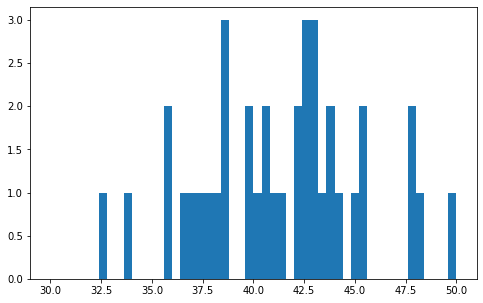
\includegraphics[width=0.7\textwidth]{figures/histo2}
	\caption{Example of histogram with custom binning and range.}
	\label{fig:histo2}
\end{figure}

Passing other parameters it is possible to modify the style of the
histogram, like its color which can be specified by name. For the basic built-in colors, you can also use a single letter

\begin{itemize}
	\tightlist
	\item
	b: blue
	\item
	g: green
	\item
	r: red
	\item
	c: cyan
	\item
	m: magenta
	\item
	y: yellow
	\item
	k: black
	\item
	w: white
\end{itemize}

Plotting multiple histograms on the same canvas is as easy as calling various times \texttt{hist} (binning should be the same for each histogram though).

To each object that is plotted can be associated a label, passing the corresponding parameter to the object call, so that we can build a legend. Latex symbols can be used whenever text is used, the characters have to be enclosed between dollar symbols (i.e. \$\\mu\$). 
The legend will be shown on the canvas with the command  \texttt{legend()}.

A grid can be added to the plot with \texttt{plt.grid(True)} for a nicer look. Figure~\ref{fig:histo3} shows such an example.

\begin{ipython}
y2 = [40.6, 40.5, 37.3, 37.6, 39.0, 38.5, 36.0, 
      39.0, 36.8, 41.4, 41.9, 39.9, 39.0, 37.7, 
      35.0, 37.9, 35.2, 39.5, 37.7, 38.4, 42.4, 
      38.1, 39.0, 34.7, 37.1, 36.6, 37.0, 40.8, 
      39.0, 41.5]

plt.hist(y1, 50, range=(30, 50), color='red', label='Red Hist')
plt.hist(y2, 50, range=(30, 50), color='yellow', label='Yellow Hist')
plt.legend()
plt.grid(True)
plt.show()
\end{ipython}

\begin{figure}[htb]
	\centering
	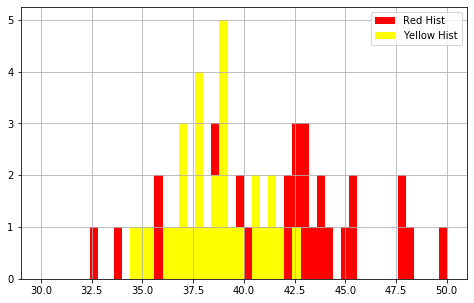
\includegraphics[width=0.7\textwidth]{figures/histo3}
	\caption{Plotting two histograms on the same canvas with different colors and the 
		corresponding legend.}
	\label{fig:histo3}
\end{figure}

\subsubsection{Scatter Plot}\label{scatter}

A scatter plot uses Cartesian coordinates to display values of two variables that are connected (e.g. date and stock price). 

Data is displayed as a collection of points, each having the value of one variable determining the position on the horizontal axis and the value of the other variable determining the position on the vertical axis. If the points are coded (color/shape/size), one additional variable can be displayed.

To create such an object call \texttt{scatter} and pass the \(x\) and \(y\) lists, Fig.~\ref{fig:scatter1}.

\begin{ipython}
y1 = [26.2, 5.4, 7.7, 3.8, 24.7, -5.5, 36.4, 12.9, 25.2, 21.0, 39.6,
      5.9, 24.8, 25.7, 42.3, 21.5, 32.3, 26.7, 37.4, 44.3, 29.0,
      52.9, 52.0, 49.5, 55.0, 40.7, 47.8, 41.1, 49.3, 58.8, 48.1,
      52.5, 51.1, 51.0, 54.3, 62.4, 52.8, 67.8, 83.6, 75.9]

x = range(len(y1))
plt.scatter(x, y1)
plt.show()
\end{ipython}

\begin{figure}[htb]
	\centering
	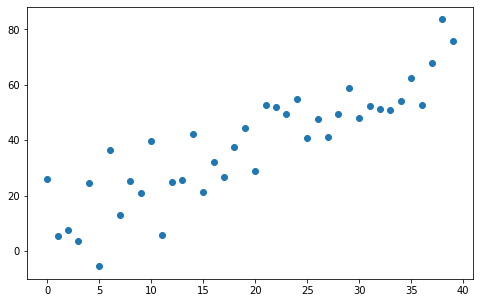
\includegraphics[width=0.7\textwidth]{figures/scatter}
	\caption{Example of scatter plot.}
	\label{fig:scatter}
\end{figure}

Other parameters can be passed to \texttt{scatter} the most useful are

\begin{itemize}
	\tightlist
	\item
	\texttt{label}: label the scatter plot for the legend;
	\item
	\texttt{color}: set the color of the marker;
	\item
	\texttt{marker}: set the style of the marker defined with a single
	character (+,*, o, x\ldots{});
	\item
	\texttt{s=}: set the size of the marker.
\end{itemize}

And of course multiple scatter plot can be shown together in the same canvas calling \texttt{scatter} accordingly (see Fig.~\ref{fig:scatter2}).

\begin{ipython}
y2 = [22.2, 3.4, 7.7, 5.8, 28.7, 0.5, 44.4, 22.9, 37.2, 35.0, 55.6,
      23.9, 44.8, 47.7, 66.3, 47.5, 60.3, 56.7, 69.4, 78.3, 65.0,
      90.9, 92.0, 91.5, 99.0, 86.7, 95.8, 91.1, 101.3, 112.8,
      104.1, 110.5, 111.1, 113.0, 118.3, 128.4, 120.8, 137.8, 155.6, 149.9]

plt.scatter(range(len(y1)), y1, s=10, marker="o",
color="lightblue", label="1st Scatter")
plt.scatter(range(len(y2)), y2, s=30, marker="*",
color="brown", label="2nd Scatter")
plt.legend()
plt.show()
\end{ipython}

\begin{figure}[htb]
	\centering
	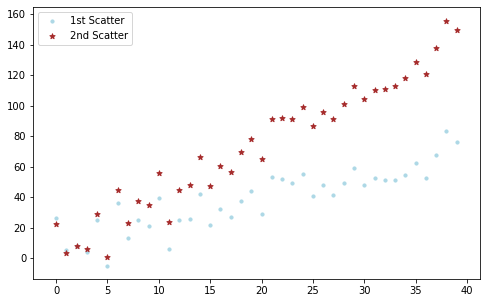
\includegraphics[width=0.65\textwidth]{figures/scatter2}
	\caption{More advanced scatter plot example.}
	\label{fig:scatter2}
\end{figure}

\subsubsection{Plot}\label{plot}

If you want to still plot \(x\) and \(y\) points but they should be connected with a line you can use the function \texttt{plot}. It acts similarly to \texttt{scatter} but the graphical result will be different.

For example below the same two scatter plots of the previous example are plotted with \texttt{plot}, Figure~\ref{fig:plot1}

\begin{ipython}
plt.plot(x, y1, label="1st Plot")
plt.plot(x, y2, label="2nd Plot")
plt.legend()
plt.show()
\end{ipython}

\begin{figure}[htb]
	\centering
	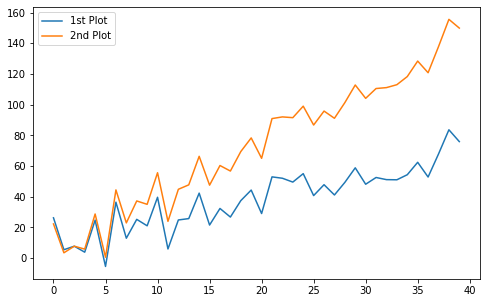
\includegraphics[width=0.65\textwidth]{figures/plot1}
	\caption{Example of scatter plot where points are connected by a line.}
	\label{fig:plot1}
\end{figure}

In this case the parameters allow to control the line style and the possibility to add the marker at each point (see Fig.~\ref{fig:plot2})

\begin{itemize}
	\tightlist
	\item
	\texttt{label}: label the scatter plot fot the legend;
	\item
	\texttt{color}: set the color of the marker and the line;
	\item
	\texttt{marker}: set the sityle of the marker defined with a single
	character (+,*, o, x\ldots{});
	\item
	\texttt{s}: set the size of the marker;
	\item
	\texttt{linestyle}: style of the line (`-', `--', `-.', `:');
	\item
	\texttt{linewidth}: thickness of the line.
\end{itemize}

\begin{ipython}
plt.plot(x, y1, marker="+", linestyle=":", color="darkgreen", label="1st Plot")
plt.plot(x, y2, marker="x", linewidth=5, color="pink", label="2nd Plot")
plt.legend()
plt.show()
\end{ipython}

\begin{figure}[htb]
	\centering
	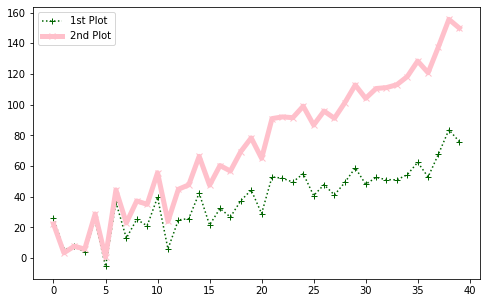
\includegraphics[width=0.7\textwidth]{figures/plot2}
	\caption{More refined example of connected scatter plot.}
	\label{fig:plot2}
\end{figure}

\subsubsection{Plotting a Function}\label{plotting-a-function}

Functions can be plotted using the \texttt{plot} method as well. They can be both functions from \texttt{python} modules or user-defined.

As an example let's try to plot \(\mathrm{sin}(x/2)\), in the example we will use \texttt{numpy.arange} function which extends the functionalities of the standard \texttt{range} allowing for non integer parameters.

In such cases it is always recommended to use \texttt{numpy} functions and not those defined in \texttt{math} since they also accept arrays in input for a faster processing (i.e. it is not need to loop over each \(x\) to compute the function values since it is done automatically).
Figure~\ref{fig:sinx_x} reports the result of the code below.

\begin{ipython}
from numpy import arange, sin

def func(x):
    return sin(x/2)
xs = arange(-10, 10, 0.01)

fig = plt.figure(figsize=(8,5))
plt.plot(xs, func(xs))
plt.show()
\end{ipython}

\begin{figure}[htb]
	\centering
	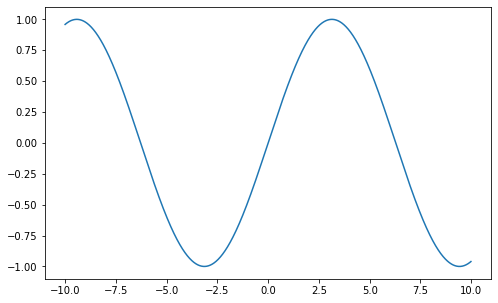
\includegraphics[width=0.65\textwidth]{figures/sinx_x}
	\caption{Example of a plot of a function, in this case \(\mathrm{sin}(x/2)\).}
	\label{fig:sinx_x}
\end{figure}

\subsection{Axes}\label{axes}

The axis of any plot can be formatted with many options.
First of all its range can be controlled with \texttt{xlim(min, max} and \texttt{ylim(min, max}. Then labels can be added with \texttt{xlabel(myLabel)} and \texttt{ylabel(myLabel)} (a global title to the plot can also be specified with \texttt{plt.title(myTitle)}).

Referring to the previous example we can write

\begin{ipython}
fig = plt.figure(figsize=(8,5))
plt.plot(x, y1, marker="+", linestyle=":", color="darkgreen", label="1st Plot")
plt.plot(x, y2, marker="x", linewidth=5, color="pink", label="2nd Plot")
plt.title("Plot Title")
plt.xlabel("x label")
plt.ylabel("y label")
plt.legend()
plt.show()
\end{ipython}
\noindent
and see the result in Fig.~\ref{fig:axis1}.

\begin{figure}[htb]
	\centering
	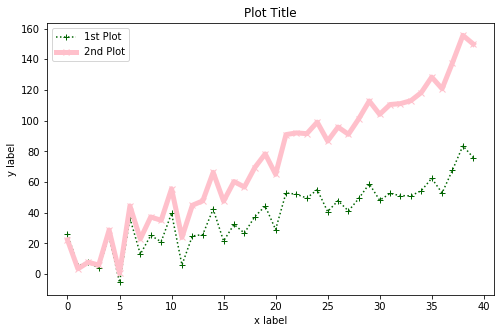
\includegraphics[width=0.65\textwidth]{figures/axis1}
	\caption{Improving the look of a plot by formatting the axis.}
	\label{fig:axis1}
\end{figure}

It can also be specified if axis has to be in linear or log scale with \texttt{xscale("log")} and/or \texttt{yscale("log")}, see Fig.~\ref{fig:axis2}.

\begin{ipython}
fig = plt.figure(figsize=(8,5))
plt.plot(x, y1, marker="+", linestyle=":", color="darkgreen", label="1st Plot")
plt.plot(x, y2, marker="x", linewidth=5, color="pink", label="2nd Plot")
plt.title("Plot Title")
plt.xlabel("x label")
plt.ylabel("y label")
plt.xscale("log")
plt.yscale("log")
plt.legend()
plt.show()
\end{ipython}

\begin{figure}[htb]
	\centering
	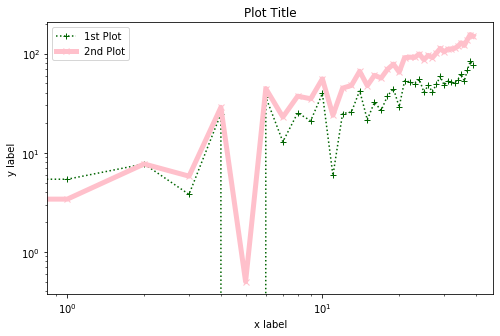
\includegraphics[width=0.7\textwidth]{figures/axis2}
	\caption{Example of log-scale plot.}
	\label{fig:axis2}
\end{figure}

\subsubsection{Date on Axis}\label{date-on-axis}

A special need, very common in finance, is to have dates on the \(x\) axis. This can be done like shown in the next example and in Figure~\ref{fig:axis3}:

\begin{ipython}
import datetime as dt
import matplotlib.dates as mdates

dates = ['01/02/1991','01/03/1991','01/04/1991']
xd = [dt.datetime.strptime(d,'%m/%d/%Y').date() for d in dates]
yd = range(len(xd))
fig = plt.figure(figsize=(8,5))
plt.gca().xaxis.set_major_formatter(mdates.DateFormatter('%m/%d/%Y'))
plt.gca().xaxis.set_major_locator(mdates.DayLocator())
plt.plot(xd, yd)
plt.gcf().autofmt_xdate() # this makes a prettier formatting
plt.show()
\end{ipython}

\begin{figure}[h]
	\centering
	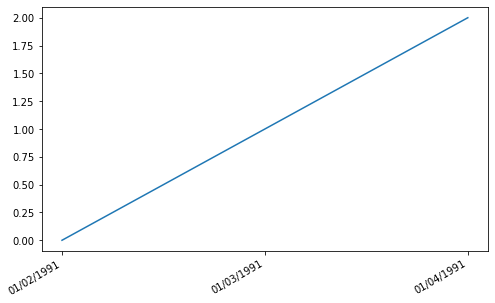
\includegraphics[width=0.6\textwidth]{figures/axis3}
	\caption{Plotting with dates on the $x$ axis.}
	\label{fig:axis3}
\end{figure}

\subsection{Subplots}
\label{subplots}

It may happen that we need to plot two or more plots side by side or in a grid fashion.

The canvas can be then split into sub-canvases with the  \texttt{subplot} commands which takes in input the number of rows, columns and the index of the current subplot. It returns the \emph{sub-canvas} object that can be used to draw like previously shown.

There is one complication though, some of the commands change when
dealing with subplots: \texttt{xlabel} and \texttt{ylabel} for example becomes \texttt{set\_xlabel} and \texttt{set\_ylabel}. Similarly for \texttt{xlim} and \texttt{ylim}.

As an example imagine that we want to plot previous data side by side on two canvases instead of together in the same (Fig.~\ref{fig:subplot})

\begin{ipython}
fig = plt.figure(figsize=(8,5))
sub1 = plt.subplot(1, 2, 1)
sub1.plot(x, y1, marker="+", linestyle=":", color="darkgreen", label="1st Plot")
sub1.set_xlabel("x label")
sub1.set_ylabel("y label")
sub1.legend()
sub2 = plt.subplot(1, 2, 2)
sub2.plot(x, y2, marker="x", linewidth=5, color="pink", label="2nd Plot")
sub2.set_xlabel("x label")
sub2.set_ylabel("y label")
sub2.legend()
plt.show()
\end{ipython}

\begin{figure} [htb]
	\centering
	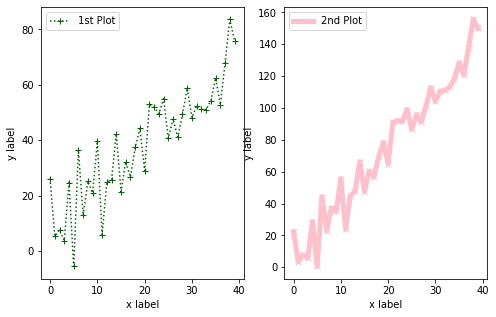
\includegraphics[width=0.65\textwidth]{figures/subplot}
	\caption{Example of subplots.}
	\label{fig:subplot}
\end{figure}

Subplots can also be arranged in another way like, see instead Figure~\ref{fig:subplot2}

\begin{ipython}
fig = plt.figure(figsize=(8,5))
sub1 = plt.subplot(2, 1, 1)
sub1.plot(x, y1, marker="+", linestyle=":", color="darkgreen", label="1st Plot")
sub1.set_xlabel("x label")
sub1.set_ylabel("y label")
sub1.legend()
sub2 = plt.subplot(2, 1, 2)
sub2.plot(x, y2, marker="x", linewidth=5, color="pink", label="2nd Plot")
sub2.set_xlabel("x label")
sub2.set_ylabel("y label")
sub2.legend()
plt.show()
\end{ipython}

%FIXME share the same axis xlabel plot 1 is covered
\begin{figure}[h]
	\centering
	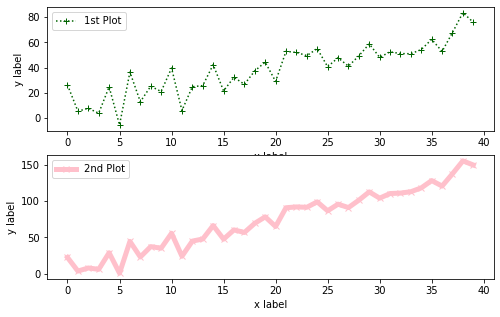
\includegraphics[width=0.65\textwidth]{figures/subplot2}
	\caption{Different arrangement of the two subplots.}
	\label{fig:subplot2}
\end{figure}

\subsection{Lines and Text}\label{lines-and-text}

To make plots more informative it can be useful to add text or lines on it.

\subsubsection{Lines}\label{lines}

Lines can be drawn with \texttt{hlines} (for horizontal lines) and
\texttt{hvines} (for vertical lines). The commands take in input the \texttt{y}, \texttt{x\_min}, \texttt{x\_max} and \texttt{x}, \texttt{y\_min}, \texttt{y\_max} respectively. Beware, coordinates are relative to the axis scale.

Other parameters allow to format the line in terms of color, style, width\ldots. Look for example at Fig.~\ref{fig:lines}

\begin{ipython}
fig = plt.figure(figsize=(8,5))
plt.plot(x, y1, marker="+", linestyle=":", color="darkgreen", label="1st Plot")
plt.plot(x, y2, marker="x", linewidth=5, color="pink", label="2nd Plot")
plt.title("Plot Title")
plt.xlabel("x label")
plt.ylabel("y label")
plt.hlines(65, 0, 37.5, color='red', linestyle="-.", label='Critical Thr.')
plt.legend()
plt.show()
\end{ipython}

\begin{figure}[htb]
	\centering
	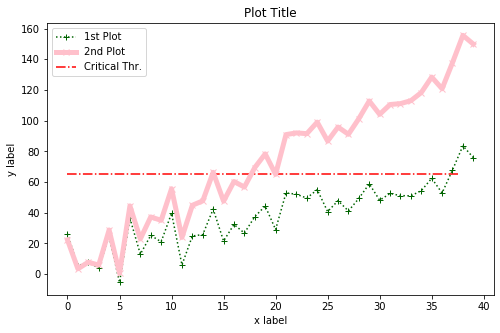
\includegraphics[width=0.7\textwidth]{figures/lines}
	\caption{Adding lines to our plots.}
	\label{fig:lines}
\end{figure}

Notice as the \(y\) value is 65 and \(x\) goes from 0 to 37.5 which corresponds to each axis.

Analogously for a vertical line, except that we have to first specify the \(x\) value and then the \(y\) range (Fig.~\ref{fig:lines2}).

\begin{ipython}
fig = plt.figure(figsize=(8,5))
plt.plot(x, y1, marker="+", linestyle=":", color="darkgreen", label="1st Plot")
plt.plot(x, y2, marker="x", linewidth=5, color="pink", label="2nd Plot")
plt.title("Plot Title")
plt.xlabel("x label")
plt.ylabel("y label")
plt.vlines(22, 0, 120, color='gray', label='Splitting Thr.')
plt.legend()
plt.show()
\end{ipython}

\begin{figure}[htb]
	\centering
	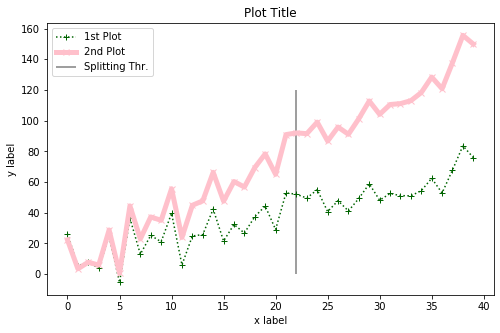
\includegraphics[width=0.7\textwidth]{figures/lines2}
	\caption{Vertical lines.}
	\label{fig:lines2}
\end{figure}

\subsubsection{Text}\label{text}

Like lines text can be added to the plot with the command \texttt{text}.
This function takes the \texttt{x} and \texttt{y} coordinates of starting point and the actual text string. Like before coordinates are relative to the axis plot.

Other options can be used to format the text style, their meaning should be straightforward:

\begin{itemize}
	\tightlist
	\item
	\texttt{backgroundcolor};
	\item
	\texttt{color};
	\item
	\texttt{fontfamily}: (FONTNAME, `serif', `sans-serif', `cursive', `fantasy', `monospace');
	\item
	\texttt{fontsize}; (size in points, `xx-small', `x-small', `small', `medium', `large', `x-large', `xx-large');
	\item
	\texttt{fontstyle}: (`normal', `italic', `oblique');
	\item
	\texttt{horizontalalignment}: (`center', `right', `left');
	\item
	\texttt{rotation}: takes the angle in degrees;
	\item
	\texttt{verticalalignment}: (`center', `top', `bottom', `baseline', `center\_baseline').
\end{itemize}

\begin{ipython}
fig = plt.figure(figsize=(8,5))
plt.plot(x, y1, marker="+", linestyle=":", color="darkgreen", label="1st Plot")
plt.plot(x, y2, marker="x", linewidth=5, color="pink", label="2nd Plot")
plt.title("Plot Title")
plt.xlabel("x label")
plt.ylabel("y label")
plt.vlines(22, 0, 120, color='gray')
plt.text(23, 5, "Splitting Thr.", rotation=90)
plt.hlines(65, 0, 37.5, color='red', linestyle="-.")
plt.text(25, 75, "Critical Thr.", backgroundcolor="red", color="white")
plt.legend()
plt.show()
\end{ipython}

\begin{figure}[htb]
	\centering
	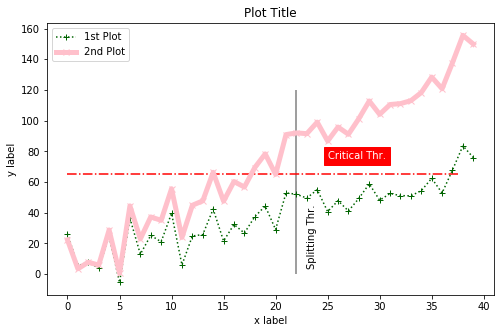
\includegraphics[width=0.7\textwidth]{figures/text}
	\caption{Adding also some text to our plot.}
	\label{fig:text}
\end{figure}

\subsection{Saving}\label{saving}

A plot can be saved into a file for later usage with \texttt{savefig} which takes in input the file name. The format of the file will be inferred from the file name extension (.jpg, .png, .gif\ldots)

\begin{ipython}
plt.savefig("myfigure.png")
\end{ipython}

%\subsection{Plot a graph given \(x\) and \(y\) values (scatter-plot)}\label{plot-a-graph-given-x-and-y-values}
%
%\begin{codebox}
%\begin{Verbatim}[commandchars=\\\{\}]
%\PY{k+kn}{from} \PY{n+nn}{matplotlib} \PY{k}{import} \PY{n}{pyplot} \PY{k}{as} \PY{n}{plt}
%
%\PY{n}{x} \PY{o}{=} \PY{p}{[}\PY{l+m+mi}{1}\PY{p}{,} \PY{l+m+mi}{2}\PY{p}{,} \PY{l+m+mi}{3}\PY{p}{]}
%\PY{n}{y} \PY{o}{=} \PY{p}{[}\PY{l+m+mf}{0.3}\PY{p}{,} \PY{l+m+mf}{0.4}\PY{p}{,} \PY{l+m+mf}{0.6}\PY{p}{]}
% 
%\PY{n}{plt}\PY{o}{.}\PY{n}{plot}\PY{p}{(}\PY{n}{x}\PY{p}{,} \PY{n}{y}\PY{p}{,} \PY{n}{marker}\PY{o}{=}\PY{l+s+s1}{\PYZsq{}}\PY{l+s+s1}{o}\PY{l+s+s1}{\PYZsq{}}\PY{p}{)} \PY{c+c1}{\PYZsh{} we are using circle markers}
%\PY{n}{plt}\PY{o}{.}\PY{n}{grid}\PY{p}{(}\PY{k+kc}{True}\PY{p}{)}               \PY{c+c1}{\PYZsh{} this line activate grid drawing}
%\PY{n}{plt}\PY{o}{.}\PY{n}{show}\PY{p}{(}\PY{p}{)}
%\end{Verbatim}
%\end{codebox}
%
%\begin{figure}[h]
%\centering
%  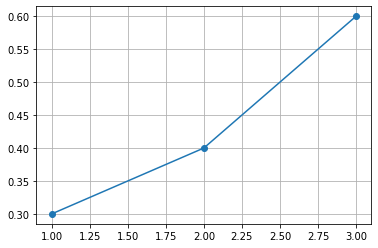
\includegraphics[width=0.6\textwidth]{figures/Untitled_43_0.png}
%\end{figure}
%%    { \hspace*{\fill} \\}
%    
%\begin{codebox}
%\begin{Verbatim}[commandchars=\\\{\}]
%\PY{c+c1}{\PYZsh{} if we want to plot specific points too}
%
%\PY{n}{x} \PY{o}{=} \PY{p}{[}\PY{l+m+mi}{1}\PY{p}{,} \PY{l+m+mi}{2}\PY{p}{,} \PY{l+m+mi}{3}\PY{p}{]}
%\PY{n}{y} \PY{o}{=} \PY{p}{[}\PY{l+m+mf}{0.3}\PY{p}{,} \PY{l+m+mf}{0.4}\PY{p}{,} \PY{l+m+mf}{0.6}\PY{p}{]}
% 
%\PY{n}{plt}\PY{o}{.}\PY{n}{plot}\PY{p}{(}\PY{n}{x}\PY{p}{,} \PY{n}{y}\PY{p}{,} \PY{n}{marker}\PY{o}{=}\PY{l+s+s1}{\PYZsq{}}\PY{l+s+s1}{x}\PY{l+s+s1}{\PYZsq{}}\PY{p}{)}
%\PY{n}{plt}\PY{o}{.}\PY{n}{plot}\PY{p}{(}\PY{l+m+mf}{2.5}\PY{p}{,} \PY{l+m+mf}{0.5}\PY{p}{,} \PY{n}{marker}\PY{o}{=}\PY{l+s+s1}{\PYZsq{}}\PY{l+s+s1}{X}\PY{l+s+s1}{\PYZsq{}}\PY{p}{,} \PY{n}{ms}\PY{o}{=}\PY{l+m+mi}{12}\PY{p}{,} \PY{n}{color}\PY{o}{=}\PY{l+s+s1}{\PYZsq{}}\PY{l+s+s1}{red}\PY{l+s+s1}{\PYZsq{}}\PY{p}{)}
%\PY{n}{plt}\PY{o}{.}\PY{n}{plot}\PY{p}{(}\PY{l+m+mf}{1.5}\PY{p}{,} \PY{l+m+mf}{0.35}\PY{p}{,} \PY{n}{marker}\PY{o}{=}\PY{l+s+s1}{\PYZsq{}}\PY{l+s+s1}{x}\PY{l+s+s1}{\PYZsq{}}\PY{p}{,} \PY{n}{ms}\PY{o}{=}\PY{l+m+mi}{12}\PY{p}{,} \PY{n}{color}\PY{o}{=}\PY{l+s+s1}{\PYZsq{}}\PY{l+s+s1}{red}\PY{l+s+s1}{\PYZsq{}}\PY{p}{)}
%\PY{n}{plt}\PY{o}{.}\PY{n}{grid}\PY{p}{(}\PY{k+kc}{True}\PY{p}{)}              
%\PY{n}{plt}\PY{o}{.}\PY{n}{show}\PY{p}{(}\PY{p}{)}
%\end{Verbatim}
%\end{codebox}
%
%\begin{figure}[h]
%\centering
%  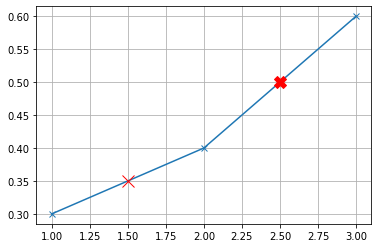
\includegraphics[width=0.6\textwidth]{figures/Untitled_44_0.png}
%\end{figure}
%%    { \hspace*{\fill} \\}
%    
%\subsubsection{What if \(x\) values are dates ?}
%
%\begin{codebox}
%\begin{Verbatim}[commandchars=\\\{\}]
%\PY{k+kn}{import} \PY{n+nn}{datetime}
%\PY{k+kn}{import} \PY{n+nn}{matplotlib}\PY{n+nn}{.}\PY{n+nn}{dates} \PY{k}{as} \PY{n+nn}{mdates}
%
%\PY{n}{x} \PY{o}{=} \PY{p}{[}\PY{n}{datetime}\PY{o}{.}\PY{n}{date}\PY{p}{(}\PY{l+m+mi}{2020}\PY{p}{,} \PY{l+m+mi}{7}\PY{p}{,} \PY{l+m+mi}{20}\PY{p}{)}\PY{p}{,}  \PY{n}{datetime}\PY{o}{.}\PY{n}{date}\PY{p}{(}\PY{l+m+mi}{2020}\PY{p}{,} \PY{l+m+mi}{7}\PY{p}{,} \PY{l+m+mi}{30}\PY{p}{)}\PY{p}{,} 
%     \PY{n}{datetime}\PY{o}{.}\PY{n}{date}\PY{p}{(}\PY{l+m+mi}{2020}\PY{p}{,} \PY{l+m+mi}{8}\PY{p}{,} \PY{l+m+mi}{10}\PY{p}{)}\PY{p}{,}  \PY{n}{datetime}\PY{o}{.}\PY{n}{date}\PY{p}{(}\PY{l+m+mi}{2020}\PY{p}{,} \PY{l+m+mi}{8}\PY{p}{,} \PY{l+m+mi}{20}\PY{p}{)}\PY{p}{]}
%     
%\PY{n}{y} \PY{o}{=} \PY{p}{[}\PY{l+m+mi}{10}\PY{p}{,} \PY{l+m+mi}{20}\PY{p}{,} \PY{l+m+mi}{34}\PY{p}{,} \PY{l+m+mi}{45}\PY{p}{]}
%\PY{n}{plt}\PY{o}{.}\PY{n}{plot}\PY{p}{(}\PY{n}{x}\PY{p}{,} \PY{n}{y}\PY{p}{,} \PY{n}{marker}\PY{o}{=}\PY{l+s+s1}{\PYZsq{}}\PY{l+s+s1}{o}\PY{l+s+s1}{\PYZsq{}}\PY{p}{)}
%\PY{c+c1}{\PYZsh{} this line tells matplotlib we have dates on x axis}
%\PY{n}{plt}\PY{o}{.}\PY{n}{gca}\PY{p}{(}\PY{p}{)}\PY{o}{.}\PY{n}{xaxis}\PY{o}{.}\PY{n}{set\PYZus{}major\PYZus{}formatter}\PY{p}{(}\PY{n}{mdates}\PY{o}{.}\PY{n}{DateFormatter}\PY{p}{(}\PY{l+s+s1}{\PYZsq{}}\PY{l+s+s1}{\PYZpc{}}\PY{l+s+s1}{Y\PYZhy{}}\PY{l+s+s1}{\PYZpc{}}\PY{l+s+s1}{m\PYZhy{}}\PY{l+s+si}{\PYZpc{}d}\PY{l+s+s1}{\PYZsq{}}\PY{p}{)}\PY{p}{)}
%\PY{c+c1}{\PYZsh{} this one instead rotate labels to avoid superimposition}
%\PY{n}{plt}\PY{o}{.}\PY{n}{xticks}\PY{p}{(}\PY{n}{rotation}\PY{o}{=}\PY{l+m+mi}{45}\PY{p}{)}
%\PY{n}{plt}\PY{o}{.}\PY{n}{grid}\PY{p}{(}\PY{k+kc}{True}\PY{p}{)}
%\PY{n}{plt}\PY{o}{.}\PY{n}{show}\PY{p}{(}\PY{p}{)}
%\end{Verbatim}
%\end{codebox}
%
%\begin{figure}[h]
%\centering
%  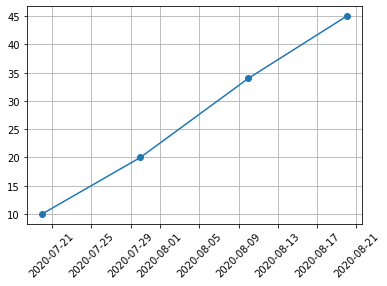
\includegraphics[width=0.6\textwidth]{figures/Untitled_46_0.png}
%\end{figure}
%%    { \hspace*{\fill} \\}
%    
%\subsection{Plotting an Histogram}\label{plotting-an-histogram}
%
%\begin{codebox}
%\begin{Verbatim}[commandchars=\\\{\}]
%\PY{k+kn}{import} \PY{n+nn}{random} 
%\PY{n}{numbers} \PY{o}{=} \PY{p}{[}\PY{p}{]}
%\PY{k}{for} \PY{n}{\PYZus{}} \PY{o+ow}{in} \PY{n+nb}{range}\PY{p}{(}\PY{l+m+mi}{1000}\PY{p}{)}\PY{p}{:}
%  \PY{n}{numbers}\PY{o}{.}\PY{n}{append}\PY{p}{(}\PY{n}{random}\PY{o}{.}\PY{n}{randint}\PY{p}{(}\PY{l+m+mi}{1}\PY{p}{,} \PY{l+m+mi}{10}\PY{p}{)}\PY{p}{)}
%
%\PY{k+kn}{from} \PY{n+nn}{matplotlib} \PY{k}{import} \PY{n}{pyplot} \PY{k}{as} \PY{n}{plt}
%
%\PY{c+c1}{\PYZsh{} Here we define the binning}
%\PY{c+c1}{\PYZsh{} 6 is the number of bins, going from 0 to 10}
%\PY{n}{plt}\PY{o}{.}\PY{n}{hist}\PY{p}{(}\PY{n}{numbers}\PY{p}{,} \PY{l+m+mi}{10}\PY{p}{,} \PY{n+nb}{range}\PY{o}{=}\PY{p}{[}\PY{l+m+mi}{0}\PY{p}{,} \PY{l+m+mi}{11}\PY{p}{]}\PY{p}{)} 
%\PY{n}{plt}\PY{o}{.}\PY{n}{show}\PY{p}{(}\PY{p}{)}
%\end{Verbatim}
%\end{codebox}
%
%\begin{figure}[h]
%\centering
%  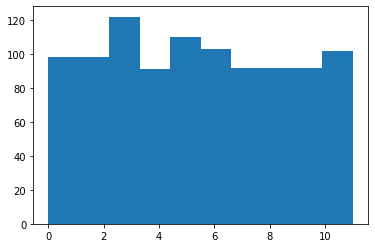
\includegraphics[width=0.55\textwidth]{figures/Untitled_48_0.png}
%\end{figure}
% %   { \hspace*{\fill} \\}
%    
%\subsubsection{Plotting a Function}\label{plotting-a-function}
%
%In this case let's try to make the plot prettier adding labels, legend\ldots{}
%All the commands apply also to the previous examples.
%
%\begin{codebox}
%\begin{Verbatim}[commandchars=\\\{\}]
%\PY{k+kn}{import} \PY{n+nn}{numpy} \PY{k}{as} \PY{n+nn}{np}
%\PY{k+kn}{import} \PY{n+nn}{matplotlib}\PY{n+nn}{.}\PY{n+nn}{pyplot} \PY{k}{as} \PY{n+nn}{plt}
%\PY{k+kn}{from} \PY{n+nn}{scipy}\PY{n+nn}{.}\PY{n+nn}{stats} \PY{k}{import} \PY{n}{norm}
%
%\PY{c+c1}{\PYZsh{} define the functions to plot}
%\PY{c+c1}{\PYZsh{} a gaussian with mean=0  and sigma=1}
%\PY{c+c1}{\PYZsh{} in scipy module this is called norm}
%\PY{n}{mu}\PY{o}{=}\PY{l+m+mi}{0}
%\PY{n}{sigma} \PY{o}{=} \PY{l+m+mi}{1}
%\PY{n}{x} \PY{o}{=} \PY{n}{np}\PY{o}{.}\PY{n}{arange}\PY{p}{(}\PY{o}{\PYZhy{}}\PY{l+m+mi}{10}\PY{p}{,} \PY{o}{\PYZhy{}}\PY{l+m+mf}{1.645}\PY{p}{,} \PY{l+m+mf}{0.001}\PY{p}{)}
%\PY{n}{x\PYZus{}all} \PY{o}{=} \PY{n}{np}\PY{o}{.}\PY{n}{arange}\PY{p}{(}\PY{o}{\PYZhy{}}\PY{l+m+mi}{4}\PY{p}{,} \PY{l+m+mi}{4}\PY{p}{,} \PY{l+m+mf}{0.001}\PY{p}{)}
%\PY{n}{y} \PY{o}{=} \PY{n}{norm}\PY{o}{.}\PY{n}{pdf}\PY{p}{(}\PY{n}{x}\PY{p}{,} \PY{l+m+mi}{0}\PY{p}{,} \PY{l+m+mi}{1}\PY{p}{)}
%\PY{n}{y\PYZus{}all} \PY{o}{=} \PY{n}{norm}\PY{o}{.}\PY{n}{pdf}\PY{p}{(}\PY{n}{x\PYZus{}all}\PY{p}{,} \PY{l+m+mi}{0}\PY{p}{,} \PY{l+m+mi}{1}\PY{p}{)}
%
%\PY{c+c1}{\PYZsh{} draw the gaussian}
%\PY{n}{plt}\PY{o}{.}\PY{n}{plot}\PY{p}{(}\PY{n}{x\PYZus{}all}\PY{p}{,} \PY{n}{y\PYZus{}all}\PY{p}{,} \PY{n}{label}\PY{o}{=}\PY{l+s+s1}{\PYZsq{}}\PY{l+s+s1}{Gaussian}\PY{l+s+s1}{\PYZsq{}}\PY{p}{)}
%
%\PY{c+c1}{\PYZsh{} fill with different alpha using x\PYZus{}all and y\PYZus{}all as limits}
%\PY{c+c1}{\PYZsh{} alpha set the transparency level: 0 trasparent, 1 solid}
%\PY{n}{plt}\PY{o}{.}\PY{n}{fill\PYZus{}between}\PY{p}{(}\PY{n}{x\PYZus{}all}\PY{p}{,} \PY{n}{y\PYZus{}all}\PY{p}{,} \PY{l+m+mi}{0}\PY{p}{,} \PY{n}{alpha}\PY{o}{=}\PY{l+m+mf}{0.1}\PY{p}{,} \PY{n}{color}\PY{o}{=}\PY{l+s+s1}{\PYZsq{}}\PY{l+s+s1}{blue}\PY{l+s+s1}{\PYZsq{}}\PY{p}{,} \PY{n}{label}\PY{o}{=}\PY{l+s+s2}{\PYZdq{}}\PY{l+s+s2}{Gaussian CDF}\PY{l+s+s2}{\PYZdq{}}\PY{p}{)}
%
%\PY{c+c1}{\PYZsh{} fill with color red using x and y as limits}
%\PY{c+c1}{\PYZsh{} label associate text to the object for the legend}
%\PY{n}{plt}\PY{o}{.}\PY{n}{fill\PYZus{}between}\PY{p}{(}\PY{n}{x}\PY{p}{,} \PY{n}{y}\PY{p}{,} \PY{l+m+mi}{0}\PY{p}{,} \PY{n}{alpha}\PY{o}{=}\PY{l+m+mi}{1}\PY{p}{,} \PY{n}{color}\PY{o}{=}\PY{l+s+s1}{\PYZsq{}}\PY{l+s+s1}{red}\PY{l+s+s1}{\PYZsq{}}\PY{p}{,} \PY{n}{label}\PY{o}{=}\PY{l+s+s2}{\PYZdq{}}\PY{l+s+s2}{5}\PY{l+s+s2}{\PYZpc{}}\PY{l+s+s2}{ tail}\PY{l+s+s2}{\PYZdq{}}\PY{p}{)}
%
%\PY{c+c1}{\PYZsh{} set x axis limits}
%\PY{n}{plt}\PY{o}{.}\PY{n}{xlim}\PY{p}{(}\PY{p}{[}\PY{o}{\PYZhy{}}\PY{l+m+mi}{4}\PY{p}{,} \PY{l+m+mi}{4}\PY{p}{]}\PY{p}{)}
%
%\PY{c+c1}{\PYZsh{} add a label for X axis}
%\PY{n}{plt}\PY{o}{.}\PY{n}{xlabel}\PY{p}{(}\PY{l+s+s2}{\PYZdq{}}\PY{l+s+s2}{Changes of value}\PY{l+s+s2}{\PYZdq{}}\PY{p}{)}
%
%\PY{c+c1}{\PYZsh{} add a label to y axis}
%\PY{n}{plt}\PY{o}{.}\PY{n}{ylabel}\PY{p}{(}\PY{l+s+s2}{\PYZdq{}}\PY{l+s+s2}{Gaussian values}\PY{l+s+s2}{\PYZdq{}}\PY{p}{)}
%
%\PY{c+c1}{\PYZsh{} add histogram title}
%\PY{n}{plt}\PY{o}{.}\PY{n}{title}\PY{p}{(}\PY{l+s+s2}{\PYZdq{}}\PY{l+s+s2}{Distribution of changes of value}\PY{l+s+s2}{\PYZdq{}}\PY{p}{)}
%
%\PY{c+c1}{\PYZsh{} draw a vertical line at x=\PYZhy{}1.645}
%\PY{c+c1}{\PYZsh{} y limits are in percent w.r.t. to y axis length}
%\PY{n}{plt}\PY{o}{.}\PY{n}{axvline}\PY{p}{(}\PY{n}{x}\PY{o}{=}\PY{o}{\PYZhy{}}\PY{l+m+mf}{1.645}\PY{p}{,} \PY{n}{ymin}\PY{o}{=}\PY{l+m+mf}{0.1}\PY{p}{,} \PY{n}{ymax}\PY{o}{=}\PY{l+m+mi}{1}\PY{p}{,} \PY{n}{linestyle}\PY{o}{=}\PY{l+s+s1}{\PYZsq{}}\PY{l+s+s1}{:}\PY{l+s+s1}{\PYZsq{}}\PY{p}{,} \PY{n}{linewidth}\PY{o}{=}\PY{l+m+mi}{1}\PY{p}{,} \PY{n}{color} \PY{o}{=} \PY{l+s+s1}{\PYZsq{}}\PY{l+s+s1}{red}\PY{l+s+s1}{\PYZsq{}}\PY{p}{)}
%
%\PY{c+c1}{\PYZsh{} write some text to explain the line}
%\PY{n}{plt}\PY{o}{.}\PY{n}{text}\PY{p}{(}\PY{o}{\PYZhy{}}\PY{l+m+mf}{1.9}\PY{p}{,} \PY{o}{.}\PY{l+m+mi}{12}\PY{p}{,} \PY{l+s+s1}{\PYZsq{}}\PY{l+s+s1}{95}\PY{l+s+s1}{\PYZpc{}}\PY{l+s+s1}{ percentile (VaR loss)}\PY{l+s+s1}{\PYZsq{}}\PY{p}{,}\PY{n}{fontsize}\PY{o}{=}\PY{l+m+mi}{10}\PY{p}{,} \PY{n}{rotation}\PY{o}{=}\PY{l+m+mi}{90}\PY{p}{,} 
%                                    \PY{n}{color}\PY{o}{=}\PY{l+s+s1}{\PYZsq{}}\PY{l+s+s1}{red}\PY{l+s+s1}{\PYZsq{}}\PY{p}{)}
%
%\PY{n}{plt}\PY{o}{.}\PY{n}{legend}\PY{p}{(}\PY{p}{)}
%\PY{n}{plt}\PY{o}{.}\PY{n}{show}\PY{p}{(}\PY{p}{)}
%\end{Verbatim}
%\end{codebox}
%
%\begin{figure}[htp]
%\centering
%  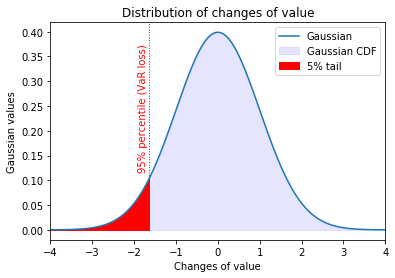
\includegraphics[width=0.55\textwidth]{figures/Untitled_50_0.png}
%\end{figure}
%%    { \hspace*{\fill} \\}
%    \clearpage
%If you are particularly satisfied by your work you can save the graph to a file:
%
%\begin{codebox}
%\begin{Verbatim}[commandchars=\\\{\}]
%\PY{n}{plt}\PY{o}{.}\PY{n}{savefig}\PY{p}{(}\PY{l+s+s1}{\PYZsq{}}\PY{l+s+s1}{normal\PYZus{}curve.png}\PY{l+s+s1}{\PYZsq{}}\PY{p}{)}
%
%<Figure size 432x288 with 0 Axes>
%
%\end{Verbatim}
%\end{codebox}

\section*{Exercises}
\begin{question}
Using \texttt{pandas} import data stored in \href{https://drive.google.com/file/d/1Uu9lQorvzM-1xwRKPNszaSqlCYAiY-gr/view?usp=sharing}{\texttt{stock\_market.xlsx}}. With the resulting dataframe determine:
\begin{itemize}
\item remove duplicates and missing data (how many rows are left ?);
\item stocks with positive variation;
\item the first five stocks with the lowest price.
\end{itemize}
\end{question}

\begin{solution}
First load the excel file into a dataframe and look at data structure.
\end{solution}

\begin{ipython}
import pandas as pd

df = pd.read_excel("stock_market.xlsx")
print (len(df))
df.head()

51

  Symbol                      Name   Price  Change  Change%  Volume (M)  \
0     GE  General Electric Company    6.07   -0.19  -0.0304     142.732
1    NOK         Nokia Corporation    4.78    0.33   0.0742     117.960
2      F        Ford Motor Company    6.61   -0.13  -0.0193     115.394
3   PINS           Pinterest, Inc.   34.29    9.10   0.3613     111.864
4   AAPL                Apple Inc.  425.04   40.28   0.1047      93.574

   Avg Volume (M)  Market Cap (B)
0         102.268          53.132
1          31.296          27.083
2          87.719          26.288
3          15.550          20.110
4          35.035        1821.000
\end{ipython}
        
As usual if we are not sure that our data is \emph{clean} we should check for duplicates and NaN and take care of them. The \texttt{duplicated} method returns the status of each row (duplicate or not, True or False). If we would like just to see the duplicated entries we could combine the \texttt{duplicated} method with the selection syntax like this:

\begin{ipython}
df[df.duplicated() == True]

   Symbol         Name  Price  Change  Change%  Volume (M)  Avg Volume (M)  \
40    RUN  Sunrun Inc.  36.69    0.02   0.0005      20.113           3.604

    Market Cap (B)
40           4.489
\end{ipython}
        
So it looks like we have just one duplicate and we can remove it:

\begin{ipython}
print ("Before duplicates removal: {}".format(len(df)))
df = df.drop_duplicates()
print ("After duplicates removal: {}".format(len(df)))

Before duplicates removal: 50
After duplicates removal: 50
\end{ipython}

Then we need to take care of the NaN, again if we want to check the rows with NaN we can select (here the syntax is a little bit more complicated since we need to use \texttt{any} to look for Nan in every column):

\begin{ipython}
df[df.isna().any(axis=1)]

   Symbol                                 Name  Price  Change  Change%  \
23   NCLH  Norwegian Cruise Line Holdings Ltd.  13.64   -0.53  -0.0374
47    NBL                   Noble Energy, Inc.    NaN   -0.23  -0.0225

    Volume (M)  Avg Volume (M)  Market Cap (B)
23      28.402          64.895             NaN
47      18.462          13.535           4.795
\end{ipython}
        
Since we don't want to artificially modify our sample we just drop rows with NaN:

\begin{ipython}
print ("Before NaN removal: {}".format(len(df)))
df = df.dropna()
print ("After NaN removal: {}".format(len(df)))

Before NaN removal: 51
After NaN removal: 49
\end{ipython}

The second point asks to determine the companies with a daily positive variation. Clearly we have to apply to the dataframe a selection on the "Change" (or "change\%") column requiring positive values.

\begin{ipython}
pos_var = df[df.loc[:, "Change"] > 0]
print (len(pos_var))
pos_var.head() # just printing the first 5 rows

16

  Symbol                         Name   Price  Change  Change%  Volume (M)  \
1    NOK            Nokia Corporation    4.78    0.33   0.0742     117.960
3   PINS              Pinterest, Inc.   34.29    9.10   0.3613     111.864
4   AAPL                   Apple Inc.  425.04   40.28   0.1047      93.574
6    BAC  Bank of America Corporation   24.88    0.04   0.0016      62.039
8     FB               Facebook, Inc.  253.67   19.17   0.0817      53.030

   Avg Volume (M)  Market Cap (B)
1          31.296          27.083
3          15.550          20.110
4          35.035        1821.000
6          72.793         215.562
8          24.521         723.726
\end{ipython}
        
So in origin we had 48 stocks and just 16 have a positive variation of its price.

The last question requires to print the first 5 stocks with the lowest prices. In this case it is enough to sort by price the dataframe (ascending) and then just select the first 5 entries.

\begin{ipython}
highest_price = df.sort_values(by=['Price'], ascending=True)[:5]
highest_price

   Symbol                      Name  Price  Change  Change%  Volume (M)  \
25   ABEV               Ambev S. A.   2.68   -0.16  -0.0563      26.136
32    BBD      Banco Bradesco S. A.   4.22   -0.32  -0.0705      22.129
1     NOK         Nokia Corporation   4.78    0.33   0.0742     117.960
15    OPK         OPKO Health, Inc.   5.15   -0.76  -0.1286      35.762
33    MRO  Marathon Oil Corporation   5.49   -0.02  -0.0036      21.249

    Avg Volume (M)  Market Cap (B)
25          36.654          41.999
32          22.046          36.739
1           31.296          27.083
15          17.792           3.450
33          34.098           4.339
\end{ipython}


\begin{question}
Given the following discount factors plot the resulting discount curve,
possibly adding axis labels and legend.
\end{question}

\begin{ipython}
dfs = [1.0, 1.0014907894567657, 1.0031038833235129, 1.0047764800189012,
       1.0065986105304596, 1.014496095021891, 1.022687560553011,
       1.0303585751965112, 1.0369440287181253, 1.0422287558021188,
       1.0461834022163963, 1.0489228953047331, 1.0505725627906783, 
       1.0513323539753632, 1.0513777790851995, 1.0508768750534248,
       1.049935905228433, 1.0486741093761602, 1.047175413484517,
       1.0455115431993336, 1.0437147446170034, 1.0418294960952215,
       1.0398823957504923, 1.0378979499878478, 1.0358789099539805,
       1.0338409767365169, 1.031791178324756, 1.0297378455884902,
       1.0276772747965244, 1.0256154380560942, 1.0235543974485939,
       1.0214974135391857, 1.0194401540150835, 1.0173862951028778]

pillars = [datetime.date(2020, 8, 3), datetime.date(2020, 11, 3),
		   datetime.date(2021, 2, 3), datetime.date(2021, 5, 3),
		   datetime.date(2021, 8, 3), datetime.date(2022, 8, 3),
		   datetime.date(2023, 8, 3), datetime.date(2024, 8, 3),
		   datetime.date(2025, 8, 3), datetime.date(2026, 8, 3),
		   datetime.date(2027, 8, 3), datetime.date(2028, 8, 3),
		   datetime.date(2029, 8, 3), datetime.date(2030, 8, 3),
		   datetime.date(2031, 8, 3), datetime.date(2032, 8, 3),
		   datetime.date(2033, 8, 3), datetime.date(2034, 8, 3),
		   datetime.date(2035, 8, 3), datetime.date(2036, 8, 3),
		   datetime.date(2037, 8, 3), datetime.date(2038, 8, 3),
		   datetime.date(2039, 8, 3), datetime.date(2040, 8, 3),
		   datetime.date(2041, 8, 3), datetime.date(2042, 8, 3),
		   datetime.date(2043, 8, 3), datetime.date(2044, 8, 3),
		   datetime.date(2045, 8, 3), datetime.date(2046, 8, 3),
		   datetime.date(2047, 8, 3), datetime.date(2048, 8, 3),
           datetime.date(2049, 8, 3), datetime.date(2050, 8, 3)]
\end{ipython}

\begin{solution}
\end{solution}

\begin{ipython}
import datetime
from matplotlib import pyplot as plt
import matplotlib.dates as mdates

dfs = [1.0, 1.0014907894567657, 1.0031038833235129, 1.0047764800189012, ...]
pillars = [datetime.date(2020, 8, 3), datetime.date(2020, 11, 3), ...]

plt.plot(pillars, dfs, marker="o", label="EUR6M d.f.")

plt.gca().xaxis.set_major_formatter(mdates.DateFormatter('%Y-%m-%d'))
# this one instead rotate labels to avoid superimposition
plt.xticks(rotation=45)
plt.xlabel("Pillar dates")
plt.ylabel("Discount Factors")
plt.grid(True)
plt.legend()
plt.show()
\end{ipython}

\begin{figure}[htb]
\begin{center}
  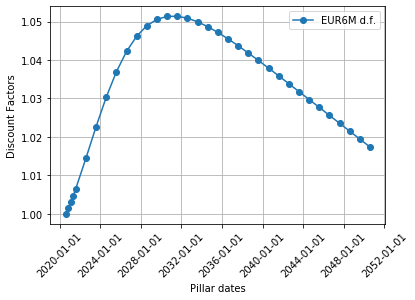
\includegraphics[width=0.7\linewidth]{figures/ex5.5.png}
\end{center}
\end{figure}





\begin{thebibliography}{9}
  %  %\bibitem{survey2019} StackOverflow \emph{The TEXbook}, Addison-Wesley, Reading,Massachusetts, second edition, 1984,
\bibitem{pandas} \href{https://pandas.pydata.org/docs/}{\emph{Pandas Official Documentation}} [Online]
\bibitem{matplotlib} \href{https://matplotlib.org}{\emph{Matplotlib Official Documentation}} [Online]
\bibitem{bib:quandl} \href{https://docs.quandl.com/}{\emph{Quandl Documentation}} [Online]
\bibitem{bib:yfinance} \href{https://github.com/ranaroussi/yfinance}{\emph{YFinance Documentation}} [Online]
\bibitem{bib:ffn} \href{https://pmorissette.github.io/ffn/}{\emph{Financial Functions for Python}} [Online]
\end{thebibliography}

\chapter{Matrices}\label{sec:matrices}

In mathematics, a matrix is a rectangular array of numbers, symbols, or expressions, arranged in rows and columns. Matrices are commonly written in box brackets. The horizontal and vertical lines of entries in a matrix are called rows and columns, respectively. The size of a matrix is defined by the number of rows and columns that it contains. A matrix with \(m\) rows and \(n\) columns is called an \(m\times n\) matrix or \(m\)-by-\(n\) matrix, while \(m\) and \(n\) are
called its dimensions. The dimensions of the following matrix are \(2\times 3\) (read ``two by three''), because there are two rows and three columns.

\[\begin{bmatrix}
1 & 2 & 3\\
4 & 5 & 6
\end{bmatrix}\]

The individual items (numbers, symbols or expressions) in a matrix are called its elements or entries. 
In \texttt{python} matrices can be represented as \texttt{numpy.array}, so the example above will become:

\begin{ipython}
import numpy as np

print (np.array([[1, 2, 3],[4, 5, 6]]))
\end{ipython}
\begin{ioutput}
[[1 2 3]
 [4 5 6]]
\end{ioutput}

Essentially a \texttt{numpy.array} is a list of lists each one representing a matrix row. Arrays can have any dimension so they can be used to represent also vectors in \texttt{python}. There are two special types of arrays: \texttt{zeros} and \texttt{ones} whose name already clarify their nature.

\begin{ipython}
A = np.zeros(shape=(3, 3))
B = np.ones(shape+(4, 4))

print (A)
print (B)
\end{ipython}
\begin{ioutput}
[[0. 0. 0.]
 [0. 0. 0.]
 [0. 0. 0.]]

[[1. 1. 1. 1.]
 [1. 1. 1. 1.]
 [1. 1. 1. 1.]
 [1. 1. 1. 1.]]
\end{ioutput}

\section{Transpose of a Matrix}
The transpose of a matrix $[A]$, denoted by $[A^T]$, may be constructed by writing the rows of $[A]$ as the columns of $[A^T]$
and the columns of $[A]$ as the rows of $[A^T]$.
Formally, the $i$-th row, $j$-th column element of $[A^T]$ is the $j$-th row, $i$-th column element of $[A]$:

\begin{equation}[A^T]_{ij} = [A]_{ji}\end{equation}

If $[A]$ is an $m\times n$ matrix, then $[A^T]$ is an $n\times m$ matrix. 
As an example the transpose of:

\[
\begin{bmatrix}
1 & 5 & 3 \\
2 & -3 & 8
\end{bmatrix}
\quad \mathrm{is} \quad
\begin{bmatrix}
1 & 2 \\
5 & -3 \\
3  & 8
\end{bmatrix}
\]

\section{Operation with Matrices}
\subsection{Adding and Subtracting Matrices}\label{adding-and-subtracting-matrices}

Usually matrices are used to list data or to represent system of equations. Since the entries are numbers, numerical operations can be performed on matrices. 
Indeed matrices can be added or subtracted by adding or subtracting corresponding entries.

In order to do this, the entries must correspond, therefore, addition
and subtraction of matrices is only possible when the matrices have the
same dimensions.

Adding two matrices is very simple. Just add each element in the first
matrix to the corresponding element in the second matrix.

\[
\begin{bmatrix}
1 & 2 & 3 \\
4 & 5 & 6
\end{bmatrix}
+
\begin{bmatrix}
10 & 20 & 30\\
40 & 50 & 60
\end{bmatrix}
=
\begin{bmatrix}
11 & 22 & 33\\
44 & 55 & 66
\end{bmatrix}
\]
As you might guess, subtracting works much the same way except that you
subtract instead of adding.

\[
\begin{bmatrix}
10 & 20 & 30\\
40 & 50 & 60
\end{bmatrix}
-
\begin{bmatrix}
1 & 2 & 3 \\
4 & 5 & 6
\end{bmatrix}
=
\begin{bmatrix}
9 & 18 & 27\\
36 & 45 & 54
\end{bmatrix}
\]
Adding and subtracting \texttt{numpy.array} is as easy as that:

\begin{ipython}
A = np.array([[1, 2, 3],[4, 5, 6]]
B = np.array([[10, 20, 30],[40, 50, 60]]

print (A + B)
print (A - B)
\end{ipython}
\begin{ioutput}
[[11 22 33]
 [44 55 66]]
 
[[ 9 18 27]
 [36 45 54]]
\end{ioutput}

\subsection{Scalar Multiplication}\label{scalar-multiplication}

Multiplying a matrix by a scalar \(c\) means you add the matrix to itself \(c\) times, or simply multiply each element by that constant.

\[
3 \cdot
\begin{bmatrix}
1 & 2 & 3 \\
4 & 5 & 6
\end{bmatrix}
=
\begin{bmatrix}
3 & 6 & 9 \\
12 & 15 & 18
\end{bmatrix}
\]
Scalar multiplication of \texttt{numpy.array} is:

\begin{ipython}
c = 3
A = np.array([[1, 2, 3],[4, 5, 6]]

print (c * A)
\end{ipython}
\begin{ioutput}
[[ 3  6  9]
 [12 15 18]]
    \end{ioutput}

\subsection{Matrix Multiplication}\label{matrix-multiplication}

Matrix multiplication is multiplying every element of each row of the first matrix times every element of each column in the second matrix. Each entry of the resultant matrix is computed one at a time.

Let's see with an example: \[ 
\begin{bmatrix}
1 & 2 \\
3 & 4
\end{bmatrix}
\cdot
\begin{bmatrix}
5 & 6 \\
7 & 8
\end{bmatrix}
= ?
\]
First ask: do the number of columns in the first matrix equal the number of rows in the second ? If so the product exists. Then start with producing the product for the first row, first column element. Take the first row of the first matrix and multiply by the first column of the second like this:

\[ 
\begin{bmatrix}
1 & 2 \\
3 & 4
\end{bmatrix}
\cdot
\begin{bmatrix}
5 & 6 \\
7 & 8
\end{bmatrix}
=
\begin{bmatrix}
(1\cdot 5) + (2\cdot 7) & X \\
X & X
\end{bmatrix}
\]
Continue the pattern with the first row of the first matrix with the second column of the second matrix:

\[ 
\begin{bmatrix}
1 & 2 \\
3 & 4
\end{bmatrix}
\cdot
\begin{bmatrix}
5 & 6 \\
7 & 8
\end{bmatrix}
=
\begin{bmatrix}
(1\cdot 5) + (2\cdot 7) & (1\cdot 6) + (2\cdot 8)  \\
X & X
\end{bmatrix}
\]
Then do the same with the second row of the first matrix and you are done:

\[ 
\begin{bmatrix}
1 & 2 \\
3 & 4
\end{bmatrix}
\cdot
\begin{bmatrix}
5 & 6 \\
7 & 8
\end{bmatrix}
=
\begin{bmatrix}
(1\cdot 5) + (2\cdot 7) & (1\cdot 6) + (2\cdot 8)  \\
(3\cdot 5) + (4\cdot 7) & (3\cdot 6) + (4\cdot 8) 
\end{bmatrix}
=
\begin{bmatrix}
19 & 22 \\
43 & 50 
\end{bmatrix}
\]
In \texttt{numpy} array multiplication can be done like this:

\begin{ipython}
A = np.array([[1, 2],[3, 4]]
B = np.array([[5, 6],[7, 8]]
	
print (np.dot(A, B))
# or equivalently A.dot(B)
\end{ipython}
\begin{ioutput}
[[19 22]
 [43 50]]
\end{ioutput}

\section{The identity matrix}\label{the-identity-matrix}

\([I]\) is defined so that \([A][I]=[A]\), i.e.~it is the matrix version of multiplying a number by one. What matrix has this property? A first guess might be a matrix full of 1s, but that does not work:

\[
\begin{bmatrix}
1 & 2 \\
3 & 4
\end{bmatrix}
\begin{bmatrix}
1 & 1 \\
1 & 1
\end{bmatrix}
=
\begin{bmatrix}
3 & 3 \\
7 & 7
\end{bmatrix}
\]
The matrix that does work is a diagonal stretch of 1s, with all other elements being 0:

\[
\begin{bmatrix}
1 & 2 \\
3 & 4
\end{bmatrix}
\begin{bmatrix}
1 & 0 \\
0 & 1
\end{bmatrix}
=
\begin{bmatrix}
1 & 2 \\
3 & 4
\end{bmatrix}
\]
So \([I] = 
\begin{bmatrix}
1 & 0 \\
0 & 1
\end{bmatrix}
\) is the identity matrix for \(2\times 2\) matrices. The \texttt{numpy} equivalent of the identity matrix is given by
\texttt{numpy.identity(n)} with \texttt{n} the dimension of the matrix. So for example:

\begin{ipython}
A = np.array([[1, 2],[3, 4]]
I = np.identity(2)	

print (A)
print (np.dot(A, I))
\end{ipython}
\begin{ioutput}
[[1 2]
 [3 4]]

[[1. 2.]
 [3. 4.]]
\end{ioutput}
    
\section{Matrix Decomposition}
\label{eigendecomposition}

Decomposing a matrix means to find a product of matrices that is equal to the initial matrix. In this Section the case of \emph{eigen-decomposition} is described, where the initial matrix is decomposed into the product of its \emph{eigenvectors} and \emph{eigenvalues}.
%Before all, let's see the link between matrices and linear
%transformation. Then, you'll learn what are eigenvectors and
%eigenvalues.

\subsection{Eigenvectors and eigenvalues}
\label{eigenvectors-and-eigenvalues}
%\subsection{Matrices as linear transformations}
%\label{matrices-as-linear-transformations}

You can think of matrices as linear transformations so some matrices will rotate your space, others will re-scale it. When a matrix is applied to a vector (apply here means calculate the dot product of the matrix with the vector), we end up with a transformed version of the vector.

Let's apply the matrix \([A]\) to a vector $\mathbf{v}$

\begin{ipython}
import numpy as np
from finmarkets import plotVectors
from matplotlib import pyplot as plt

A = np.array([[1, 3], [2, 2]])	
v = np.array([2, 1])
Av = A.dot(v)

plotVectors([v.flatten({}, Av.flatten()], cols=["1190FF", "FF9A13"])
plt.ylim(1, 4)
plt.xlim(1, 4)
\end{ipython}
\begin{ioutput}
(-1.0, 4.0)
\end{ioutput}

Figure~\ref{fig:matrix_as_transform} shows the effect of the application of the matrix to the vector, the new vector (orange) has a different direction than the original one (light blue).

\begin{figure}[htb]
	\centering
	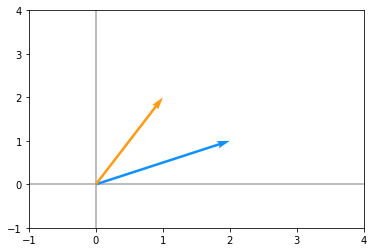
\includegraphics[width=0.7\linewidth]{figures/matrix_transformation}
	\caption{Application of a matrix to a vector, the new vector (orange) is different than the original one (blue).}
	\label{fig:matrix_as_transform}
\end{figure}


%We have seen an example of a vector transformed by a matrix. Now
%imagine that the transformation of the initial \%vector gives us a new
%vector that has the exact same direction. The scale can be different but
%the direction is the \%same. Applying the matrix doesn't change the
%direction of the vector. This special vector is called an eigenvector of
%\%the matrix.

Now imagine that the transformation of the initial vector by the matrix gives a new vector with the exact same direction. This vector is called an \emph{eigenvector} of \([A]\).

This means that \textbf{v} is a eigenvector of \([A]\) if \textbf{v} and \([A]\mathbf{v}\) (the transformed vector) have the same direction. The output vector is just a scaled version of the input one with the scaling factor \(\lambda\) which is called an \emph{eigenvalue} of \([A]\). Mathematically, the following equation holds:

\begin{equation}
[A]\mathbf{v}=\lambda \mathbf{v}
\end{equation}

\subsection{Finding Eigenvalues and Eigenvectors in \texttt{python}}
\label{find-eigenvalues-and-eigenvectors-in-python}

\texttt{numpy} provides a function returning eigenvectors and eigenvalues: 

\begin{ipython}
A = np.array([[5, 1], [3, 3]])
np.linalg.eig(A)
\end{ipython}
\begin{ioutput}
(array([6., 2.]),

array([[ 0.70710678, -0.31622777],
       [ 0.70710678,  0.9486833 ]]))
\end{ioutput}
The eigenvectors correspond to the columns of the second array. This means that the eigenvector corresponding to \(\lambda=6\) is:

\[\begin{bmatrix}
0.70710678 \\
0.70710678\end{bmatrix}\]
while the eigenvector corresponding to \(\lambda=2\) is:

\[\begin{bmatrix}
−0.31622777 \\
0.9486833\end{bmatrix}\]

It is important to note that there exists an infinite number of eigenvectors corresponding to a given eigenvalue, they are equivalent because they have the same direction but are just scaled differently. For example the first eigenvector found above is a scaled version of \(\begin{bmatrix}1\\ 1\end{bmatrix}\).

\begin{ipython}
v = np.array([1, 2])
Av = A.dot(v)
v_np = [0.31622777, 0.9486833]	
\end{ipython}
\begin{ioutput}
(-1.0, 3.0)
\end{ioutput}
Figure~\ref{fig:eigenvectors} shows three equivalent eigenvectors found
with the code above. We can see that the vector found with \(\tt{numpy}\) (in dark blue) is a scaled version of \(\begin{bmatrix}1\\ -3\end{bmatrix}\).

\begin{figure}[htb]
	\centering
	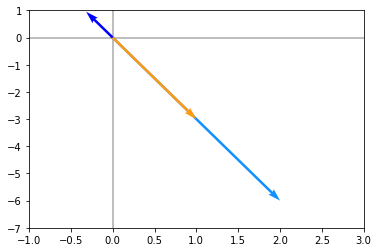
\includegraphics[width=0.7\linewidth]{figures/eigenvectors}
	\caption{Graphical representation of three equivalent eigenvectors.}
	\label{fig:eigenvectors}
\end{figure}

%Let's \([A]\) be the following matrix:
%
%\[A=\begin{bmatrix}
%5 &1 \\
%3 &3
%\end{bmatrix}\]
%
%We know that one eigenvector of A is:
%
%\[v=\begin{bmatrix}
%1 \\
%1\end{bmatrix}\] We can check that \([A]v=\lambda v\)
%
%\[\begin{bmatrix}
%5 & 1 \\
%3& 3\end{bmatrix}
%\begin{bmatrix}
%1 \\
%1\end{bmatrix}
%=\begin{bmatrix}
%6 \\
%6\end{bmatrix}\]
%
%We can represent \(v\) and \([A]v\) to check if their directions are the
%same:
%
%\begin{codebox}
%	\begin{Verbatim}[commandchars=\\\{\}]
%	\PY{n}{A} \PY{o}{=} \PY{n}{np}\PY{o}{.}\PY{n}{array}\PY{p}{(}\PY{p}{[}\PY{p}{[}\PY{l+m+mi}{5}\PY{p}{,} \PY{l+m+mi}{1}\PY{p}{]}\PY{p}{,} \PY{p}{[}\PY{l+m+mi}{3}\PY{p}{,} \PY{l+m+mi}{3}\PY{p}{]}\PY{p}{]}\PY{p}{)}
%	\PY{n}{v} \PY{o}{=} \PY{n}{np}\PY{o}{.}\PY{n}{array}\PY{p}{(}\PY{p}{[}\PY{p}{[}\PY{l+m+mi}{1}\PY{p}{]}\PY{p}{,} \PY{p}{[}\PY{l+m+mi}{1}\PY{p}{]}\PY{p}{]}\PY{p}{)}
%	
%	\PY{n}{Av} \PY{o}{=} \PY{n}{A}\PY{o}{.}\PY{n}{dot}\PY{p}{(}\PY{n}{v}\PY{p}{)}
%	
%	\PY{n}{orange} \PY{o}{=} \PY{l+s+s1}{\PYZsq{}}\PY{l+s+s1}{\PYZsh{}FF9A13}\PY{l+s+s1}{\PYZsq{}}
%	\PY{n}{blue} \PY{o}{=} \PY{l+s+s1}{\PYZsq{}}\PY{l+s+s1}{\PYZsh{}1190FF}\PY{l+s+s1}{\PYZsq{}}
%	
%	\PY{n}{plotVectors}\PY{p}{(}\PY{p}{[}\PY{n}{Av}\PY{o}{.}\PY{n}{flatten}\PY{p}{(}\PY{p}{)}\PY{p}{,} \PY{n}{v}\PY{o}{.}\PY{n}{flatten}\PY{p}{(}\PY{p}{)}\PY{p}{]}\PY{p}{,} \PY{n}{cols}\PY{o}{=}\PY{p}{[}\PY{n}{blue}\PY{p}{,} \PY{n}{orange}\PY{p}{]}\PY{p}{)}
%	\PY{n}{plt}\PY{o}{.}\PY{n}{ylim}\PY{p}{(}\PY{o}{\PYZhy{}}\PY{l+m+mi}{1}\PY{p}{,} \PY{l+m+mi}{7}\PY{p}{)}
%	\PY{n}{plt}\PY{o}{.}\PY{n}{xlim}\PY{p}{(}\PY{o}{\PYZhy{}}\PY{l+m+mi}{1}\PY{p}{,} \PY{l+m+mi}{7}\PY{p}{)}
%
%(-1.0, 7.0)
%\end{Verbatim}
%\end{codebox}
%
%\begin{center}
%	\adjustimage{max size={0.9\linewidth}{0.9\paperheight}}{eigenvectors_files/eigenvectors_3_1.png}
%\end{center}
%
%We can see that their directions are the same!
%
%This example shows that the eigenvectors \(v\) are vectors that change
%only in scale when we apply the matrix \([A]\) to them.

\section{The Inverse of a Matrix}\label{the-inverse-of-a-matrix}

The inverse of matrix \([A]\) is \([A^{-1}]\), and is defined by the property:

\begin{equation} [A][A^{-1}]=[I] \end{equation}

Hence the matrix \([B]\) is the inverse of the matrix \([A]\) if when multiplied together, \([A][B]\) gives the identity matrix. 
Using the definition let's try to find the inverse of:

\[
\begin{bmatrix}
3 & 4\\
5 & 6
\end{bmatrix}
\]
First, let the following be true:

\[
\begin{bmatrix}
3 & 4\\
5 & 6
\end{bmatrix}
\begin{bmatrix}
a & b\\
c & d
\end{bmatrix}
=
\begin{bmatrix}
1 & 0\\
0 & 1
\end{bmatrix}
\]
When multiplying this mystery matrix by our original matrix, the result is

\[
\begin{bmatrix}
3a+4c & 3b+4d\\
5a+6c & 5b+6d
\end{bmatrix}
=
\begin{bmatrix}
1 & 0\\
0 & 1
\end{bmatrix}
\]
For two matrices to be equal, every element on the left must equal its corresponding element on the right. So, for these two matrices to equal each other:

\[
\begin{cases}
3a+4c=1\\
3b+4d=0\\
5a+6c=0\\
5b+6d=1
\end{cases}
\]
Solving this simple system we get the following result:

\[
\begin{cases}
a=−3\\
b=2\\
c=2.5\\
d=−1.5
\end{cases}
\]
Having solved for the four variables, the result is the inverse

\[
\begin{bmatrix}
−3 & 2\\
2.5 & −1.5
\end{bmatrix}
\]
The quick check to be sure the result is correct is done in \texttt{python}. The \texttt{linalg.inv()} function can be used to find the inverse of a matrix:

\begin{ipython}
from numpy,linalg import inv

A = np.array([[3, 4],[5, 6]])	
print (inv(A))
\end{ipython}
\begin{ioutput}
[[-3.   2. ]
 [ 2.5 -1.5]]
\end{ioutput}

\subsection{The Moore-Penrose Pseudo-inverse}
\label{the-moore-penrose-pseudoinverse}

%The Moore-Penrose pseudo-inverse is a direct application of the SVD. But
%before all, we have to remind that systems of equations can be expressed
%under the matrix form.
The Moore-Penrose pseudo-inverse is \([A^+]\) such as:

\[[A][A^+]≈[I]\]

Think of it as a generalization of the inverse. It is defined for all matrices, but has fewer guaranteed properties as a result. For example, it will be a matrix such that \([𝐴][𝐴^+][𝐴]=[𝐴]\), but not necessarily the stronger usual inverse property is true \([𝐴^{−1}][𝐴]=[𝐴][𝐴^{−1}]=[𝐼]\) (the second one implies the first). In the special case where a matrix has an inverse, it will be the same as the pseudo-inverse.

%So pinv() gives you the inverse where it exists, and still gives
%something inverse-like everywhere else.

%The pseudo-inverse is the ``closest'' answer to \([𝐴]\mathbf{x}=[𝐼]\), in the sense that the norm \(||[𝐴][𝑋]−[𝐼]||_2\) is smallest. It's 0 when the
%inverse exists of course.

Let's create a non square matrix $[A]$, calculate its singular value decomposition and its pseudo-inverse with  \texttt{linalg.pinv()}.

\[A=\begin{bmatrix}
7&2\\
3&4\\
5&3\end{bmatrix}\]

\begin{ipython}
A = np.array([[7, 2, 3],[4, 5, 3]])
A = np.linalg.pinv(A)
A_plus = np.linalg.pinv(A)
print (A_plus)
\end{ipython}
\begin{ioutput}
[[ 0.16666667 -0.10606061  0.03030303]
 [-0.16666667  0.28787879  0.06060606]]
\end{ioutput}
It can be checked that it is really the near inverse of $[A]$ since we know that

\[[A^{+}][A]\approx[A^{−1}][A]=[I]\]

\begin{ipython}
A_plus.dot(A)
\end{ipython}
\begin{ioutput}
array([[1.00000000e+00, 2.35922393e-16],
       [3.33066907e-16, 1.00000000e+00]])
\end{ioutput}
This is almost the identity matrix! Another difference with respect to the real inverse is that \([A^+][A]≈[I]\) but \([A][A^+]\neq [I]\).

\subsection{Eigen-decomposition}
\label{concatenating-eigenvalues-and-eigenvectors}

Now that we have an idea of what eigenvectors and eigenvalues are, we
can see how it can be used to decompose a matrix. 
Then the \emph{eigen-decomposition} is given by

\begin{equation}
[A]=[V]\cdot \textrm{diag}(\boldsymbol{\lambda})\cdot [V^{−1}]
\end{equation}
where the matrix $[V]$ is made by concatenating all eigenvectors
of $[A]$ in each column (like in the second array returned by
\(\tt{np.linalg.eig(A))}\), \(\textrm{diag}(\boldsymbol{\lambda})\) 
is a diagonal matrix containing all the eigenvalues.
Continuing with our example above we have

\[V=\begin{bmatrix}
1 & 1 \\
1 &−3\end{bmatrix}\qquad 
\textrm{diag}(\boldsymbol{\lambda})=\begin{bmatrix}
6&0\\
0&2\end{bmatrix}\] 
and the inverse matrix of \([V]\) can be calculated with
\(\tt{numpy}\)

\begin{ipython}
V = np.array([[1, 1], [1, 3]])
V_inv = np.linalg.inv(V)
print (V_inv)
\end{ipython}
\begin{ioutput}
array([[ 0.75,  0.25],
       [ 0.25, -0.25]])
\end{ioutput}

So let's plug it into our equation:

\[ [V]\cdot\textrm{diag}(\boldsymbol{\lambda})\cdot [V^{−1}]=
\begin{bmatrix}
1 & 1 \\
1 &−3\end{bmatrix}
\begin{bmatrix}
6&0\\
0&2\end{bmatrix}
\begin{bmatrix}
0.75 & 0.25\\
0.25&-0.25 \end{bmatrix}
=\begin{bmatrix}
5 & 1\\
3& 3\end{bmatrix}
\]

Let's check our result with \texttt{python}

\begin{ipython}
lambdas = np.diag([6, 2])	
V.dot(lambdas).dot(V_inv)
\end{ipython}
\begin{ioutput}
array([[5., 1.],
       [3., 3.]])
\end{ioutput}

\subsubsection{Real symmetric matrix}
\label{real-symmetric-matrix}

In the case of real symmetric matrices (\([A]=[A^T]\)) the
eigen-decomposition can be expressed as

\begin{equation}
[A]=[Q][\Lambda][Q^T]
\end{equation} 
where \([Q]\) is the matrix with eigenvectors as columns and \(\Lambda\) is \(\textrm{diag}(\boldsymbol{\lambda})\).

For that reason, it can useful to use symmetric matrices! Let's do it now with \(\tt{linalg}\) from \(\tt{numpy}\)

\begin{ipython}
A = np.array([[6, 2], [2, 3]])

eigVals, eigVecs = np.linalg.eig(A)
eigVals = np.diag(eigVals)

print (eigVecs.dot(eigVals).dot(eigVecs.T))
\end{ipython}
\begin{ioutput}
array([[6., 2.],
       [2., 3.]])
\end{ioutput}

%\subsubsection{Quadratic form to matrix form}
%\label{quadratic-form-to-matrix-form}
%
%Let's have the following quadratic equation:
%
%\[f(x)=ax^2_1+(b+c)x_1x_2+dx^2_2\] These quadratic forms can be
%generated by matrices:
%
%\[f(x)=
%\begin{bmatrix}
%x_1 & x_2
%\end{bmatrix}
%\begin{bmatrix}
%a&b\\
%c&d
%\end{bmatrix}
%\begin{bmatrix}
%x_1\\
%x_2\end{bmatrix}
%=x^T[A]x\]
%
%\subsection{With the Principal Axes Theorem}
%\label{with-the-principal-axes-theorem}
%
%Actually there is a simpler way to do the change of variable. We can
%stay in the matrix form. Recall that we start with the form:
%
%\[f(x)=x^T[A]x\] The linear substitution can be wrote in these terms. We
%want replace the variables \(x\) by \(y\) that relates by:
%
%\[x=[P]y\] We want to find \([P]\) such as our new equation doesn't
%contain the cross terms. The first step is to replace that in the first
%equation:
%
%\[x^T[A]x=([P]y)^T[A]([P]y)=y^T([P]^T[A][P])y\] Can you see the how to
%transform the left hand side (\(x\)) into the right hand side (\(y\))?
%The substitution is done by replacing \([A]\) with \([P]^T[A][P]\). We
%also know that \([A]\) is symmetric and thus that there is a diagonal
%matrix \([D]\) containing the eigenvectors of \([A]\) and such as
%\([D]=[P]^T[A][P]\). We thus end up with:
%
%\[x^T[A]x=y^T[D]y\] All of this implies that we can use \([D]\) to
%simplify our quadratic equation and remove the cross terms. If you
%remember from example 2 we know that the eigenvalues of \([A]\) are:
%
%\[[D]=\begin{bmatrix}
%7 &0\\
%0 &2\end{bmatrix}\]
%
%\[x^T[A]x=y^T[D]y=y^T
%\begin{bmatrix}
%7 &0\\
%0 &2\end{bmatrix}y=
%\begin{bmatrix}y_1 & y_2\end{bmatrix}
%\begin{bmatrix}
%7 &0\\
%0 &2\end{bmatrix}
%\begin{bmatrix}y_1\\y_2\end{bmatrix}
%=\begin{bmatrix}7y_1+0y_2 & 0y_1+2y_2\end{bmatrix}
%\begin{bmatrix}y_1\\y_2\end{bmatrix}=7y^2_1+2y^2_2
%\]
%
%This form (without cross-term) is called the principal axes form.
%
%\subsection{Quadratic form optimization}
%\label{quadratic-form-optimization}
%
%Depending to the context, optimizing a function means finding its
%maximum or its minimum. It is for instance widely used to minimize the
%error of cost functions in machine learning.
%
%Here we will see how eigendecomposition can be used to optimize
%quadratic functions and why this can be done easily without cross terms.
%The difficulty is that we want a constrained optimization, that is to
%find the minimum or the maximum of the function for \(f(x)\) being a
%unit vector.
%
%\paragraph{Example 8.}\label{example-8.}
%
%We want to optimize:
%
%\(f(x)=x^T[A]x\) subject to \(||x||_2=1\).In our last example we ended
%up with:
%
%\(f(x)=7y^2_1+2y^2_2\) And the constraint of \(x\) being a unit vector
%imply:
%
%\[||x||_2=1 \implies x^2_1+x^2_2=1\] We can also show that \(y\) has to
%be a unit vector if it is the case for \(x\). Recall first that
%\(x=[P]y\):
%
%%\[||x||_2=$x^Tx=([P]y)^T([P]y)=y^T[P]^T[P]y=y^Ty=||y||_2\] So
%\(||x||_2=||y||_2=1\) and thus \(y^2_1+y^2_2=1\) Since \(y^2_1\) and
%\(y^2_2\) cannot be negative because they are squared values, we can be
%sure that \(2y^2_2\leq 7y^2_2\). Hence:
%
%\[f(x)=7y^2_1+2y^2_2\leq 7y^2_1+7y^2_2 \leq 7(y^2_1+y^2_2)\leq7\] This
%means that the maximum value of \(f(x)\) is 7.
%
%The same way can lead to find the minimum of \(f(x)\).
%\(7y^2_1\geq 2y^2_1\) and:
%
%\[f(x)=7y^2_1+2y^2_2\geq2y^2_1+2y^2_2\geq2(y^2_1+y^2_2)\geq2\] And the
%minimum of \(f(x)\) is 2.

\section{Matrix Equations}\label{matrix-equations}
As we have learned in previous Sections,
matrices can be manipulated in any way that a normal equation can be.
Here it will be shown how matrices can be used to compactly write and work with systems of
multiple linear equations. 

\subsection{Writing a System of Equations with Matrices}\label{writing-a-system-of-equations-with-matrices}

It is possible to solve a system of equations using the elimination or
substitution method, but it is also possible to do it with a matrix
operation. Before we start setting up the matrices, it is important to
do the following:

\begin{itemize}
\tightlist
\item
  make sure that all of the equations are written in a similar manner,
  meaning the variables need to all be in the same order;
\item
  make sure that one side of the equation is only variables and their
  coefficients, and the other side is just constants;
\end{itemize}

Using matrix multiplication, we may define a
system of equations with the same number of equations as variables as:

\begin{equation} 
[A]\mathbf{x} = [B]
\end{equation}
where \([A]\) is the coefficient matrix, \(\mathbf{x}\) is the variable matrix, and \([B]\) is the constant matrix. Given the system:

\[
\begin{cases}
x + 8y = 7 \\
2x -8y = -3
\end{cases}
\]
the corresponding matrices are

\[[A]=
\begin{bmatrix}
1 & 8\\
2 & -8
\end{bmatrix}
;\quad
\mathbf{x}=
\begin{bmatrix}
x\\
y
\end{bmatrix}
;\quad
[B]=
\begin{bmatrix}
7\\
-3
\end{bmatrix}
\]

\subsection{Solving Systems of Equations Using Matrix Inverses}\label{solving-systems-of-equations-using-matrix-inverses}

A system of equations can be readily solved using the concepts of the inverse matrix and matrix multiplication.
Indeed to solve a system $[A]\mathbf{x}=[B]$, for $\mathbf{x}$, multiply both sides by the inverse of $[A]$

\begin{equation}
[A^{-1}][A]\mathbf{x}=[A^{-1}][B] \implies \mathbf{x} = [A^{-1}][B]
\label{eq:matrix_solution} 
\end{equation}

Provided the inverse \([A^{-1}]\) exists, Eq.~\ref{eq:matrix_solution} will solve the system. If the coefficient matrix is not invertible, the system could be inconsistent and have no solution, or be dependent and have infinitely many solutions.

Solve the following system of linear equations:

\[
\begin{cases}
x+2y-z=11\\
2x-y+3z=7\\
7x-3y-2z=2
\end{cases}
\]
Set up the three necessary matrices:

\[[A]=
\begin{bmatrix}
1 & 2 & -1 \\ 
2 & -1 & 3 \\
7 & -3 & -2
\end{bmatrix}
;\quad
[B]=
\begin{bmatrix}
11\\
7\\
2
\end{bmatrix}
;\quad
\mathbf{x}=
\begin{bmatrix}
x\\
y \\ 
z
\end{bmatrix}
\]
Since to solve this system we have to find the inverse matrix of \([A]\) and multiply it to \([B]\) we have all the ingredients to do it in \texttt{python}:

\begin{ipython}
A = np.array([[1, 2, 1], [2, 1, 3],[7, 3, 2]])
B = np.array([11, 7, 2])

A_inv = inv(A)
sol = np.dot(A_inv, B)

print (sol)
\end{ipython}
\begin{ioutput}
[3. 5. 2.]
\end{ioutput}

So the solution of the system is: \[
\begin{cases}
x=3\\
y=5\\
z=2
\end{cases}
\]

\subsection{Solving Over-determined Systems}
\label{using-the-pseudoinverse-to-solve-a-overdetermined-system-of-linear-equations}

As we have seen the inverse of a matrix \([A]\) can be used to solve the equation \([A]\mathbf{x}=[B]\). But in the case where the set of equations have 0 or many solutions the inverse cannot be found and the equation cannot be solved. 

The pseudo-inverse helps to solve the system returning the solution that minimize the error (i.e. the solution which gives the closest result to 
0 for each equation in the system). 

For this example we will consider this set of three equations with two
unknowns:

\[
\begin{cases}
−2x_1−x_2=−2 \\
4x_1−x_2=−8 \\
−x_1−x_2=−2 
\end{cases}\]

%\begin{codebox}
%\begin{Verbatim}[commandchars=\\\{\}]
%\PY{n}{x1} \PY{o}{=} \PY{n}{np}\PY{o}{.}\PY{n}{linspace}\PY{p}{(}\PY{o}{\PYZhy{}}\PY{l+m+mi}{5}\PY{p}{,} \PY{l+m+mi}{5}\PY{p}{,} \PY{l+m+mi}{1000}\PY{p}{)}
%\PY{n}{x2\PYZus{}1} \PY{o}{=} \PY{o}{\PYZhy{}}\PY{l+m+mi}{2}\PY{o}{*}\PY{n}{x1} \PY{o}{+} \PY{l+m+mi}{2}
%\PY{n}{x2\PYZus{}2} \PY{o}{=} \PY{l+m+mi}{4}\PY{o}{*}\PY{n}{x1} \PY{o}{+} \PY{l+m+mi}{8}
%\PY{n}{x2\PYZus{}3} \PY{o}{=} \PY{o}{\PYZhy{}}\PY{l+m+mi}{1}\PY{o}{*}\PY{n}{x1} \PY{o}{+} \PY{l+m+mi}{2}
%\end{Verbatim}
%\end{codebox}

Figure~\ref{fig:overdet_system} shows a graphical representation of each equation. Being an over-determined system the three lines don't intersect in a single point. Putting this into the matrix form we have:

\[[A]=\begin{bmatrix}
−2&-1\\
4&-1\\
−1&−1\end{bmatrix}\quad 
\mathbf{x}=\begin{bmatrix}
x_1\\
x_2\end{bmatrix}\quad
[B]=\begin{bmatrix}
−2\\
−8\\
−2\end{bmatrix}\]

\[[A]\mathbf{x}=[B]\implies 
\begin{bmatrix}
−2&-1\\
4&-1\\
−1&−1\end{bmatrix}
\begin{bmatrix}
x_1\\
x_2\end{bmatrix}=
\begin{bmatrix}
−2\\
−8\\
−2\end{bmatrix}\]

We will now calculate the pseudo-inverse of \([A]\):

\begin{ipython}
A = np.array([[2, 1], [4, 1], [1, 1]])
A_plus = np.linalg.pinv(A)

print (A_plus)
\end{ipython}
\begin{ioutput}
array([[-0.11290323,  0.17741935, -0.06451613],
       [-0.37096774, -0.27419355, -0.35483871]])
\end{ioutput}

Now that we have calculated the pseudo-inverse of \([A]\) we can use it to find \(\mathbf{x}\) knowing that: \(\mathbf{x}=[A^+] [B]\)

\begin{ipython}
b = np.array([[2], [8], [2]])
res = A_plus.dot(b)
print (res)
\end{ipython}
\begin{ioutput}
array([[-1.06451613],
       [ 3.64516129]])
\end{ioutput}

In our two dimensions, these are the coordinates of \(\mathbf{x}\). In Fig.~\ref{fig:overdet_system} this point, representing our "best" solution is plotted.

\begin{figure}[htb]
	\centering
	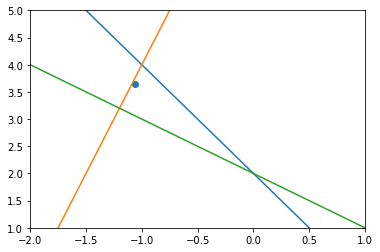
\includegraphics[width=0.7\linewidth]{figures/overdet_system}
	\caption{The three lines represent our system of equation, the point 
		the solution found with the pseudo-inverse technique.}
	\label{fig:overdet_system}
\end{figure}

Maybe you would have expected the point being at the barycentre of the triangle, well this is not the case because the equations are not scaled the same way.


%To me the important property of the pseudo-inverse arises in solving a
%simple linear system of equations. It has 0, 1, or infinitely many
%solutions. \(𝑥=[𝐴]^+𝑏\) is the closest solution when none exists in the
%sense above. It gives the single answer when 1 exists. And when many
%exists, it is the smallest solution in the sense that \(||𝑥||_2\) is
%smallest.

\section{Principal Components Analysis}
\label{sec:pca}

Principal Component Analysis, or PCA, is a dimensionality-reduction method that is often used to reduce the complexity of large datasets, by transforming the original set of variables into a smaller one that still contains most of the initial information.

Reducing the number of variables of a dataset naturally comes at the expense of accuracy. Since smaller datasets are easier to explore and visualize, and make analyzing data simpler and faster without extraneous variables to process, the trick is to trade less accuracy for more simplicity

Let's see how this kind of technique can be implemented starting from 
a multidimensional initial dataset 
\begin{equation}
X=\begin{bmatrix}
x^{(1)}_1 &x^{(2)}_1&\cdots &x^{(m)}_1 \\
x^{(1)}_2 &x^{(2)}_2&\cdots &x^{(m)}_2 \\
\vdots &\vdots &\vdots &\vdots \\
x^{(1)}_n &x^{(2)}_n&\cdots &x^{(m)}_n 
\end{bmatrix}
\end{equation}

To allow an easier representation in the examples of this Section we will use the following two-dimensional dataset.

\begin{ipython}
import numpy as np
from matplotlib import pyplot as plt
	
np.random.seed(123)
x = 5*np.random.rand(100)
y = 2*x + 1 + np.random.rand(100)

x = x.reshape(100, 1)	
y = y,hstack([x, y])
\end{ipython}

Left plot of Fig.~\ref{fig:pca_dataset} shows the dataset.

\subsection{Standardization}
The first step to implement PCA is to standardize the range of the variables so that each one of them contributes equally.

More specifically, the reason why it is critical to perform \emph{standardization} prior to PCA, is that the latter is sensitive to the variances of the initial variables. That is, if there are large differences between the ranges of the variables, those with larger ranges will dominate over those with small ranges (e.g. a variable that goes from 0 and 100 will dominate over another one that ranges between 0 and 1), which will lead to biased results. 

Mathematically, this can be done by subtracting the mean and dividing by the standard deviation for each component of each variable

\begin{equation}
z = \cfrac{x - \textrm{mean}}{\textrm{std dev.}}
\end{equation}

Once the standardization is done, all the variables will be transformed to the same scale.

\begin{ipython}
def centerDate(X):
    X = X.copy()
    X = (X - np.mean(X, axis=0)/np.std(X, axis=0)
    return X
    
X_centered = centerData(X)
\end{ipython}

Right plot of Fig.~\ref{fig:pca_dataset} shows the standardized dataset used in the following.

\begin{figure}[htb]
	\centering
	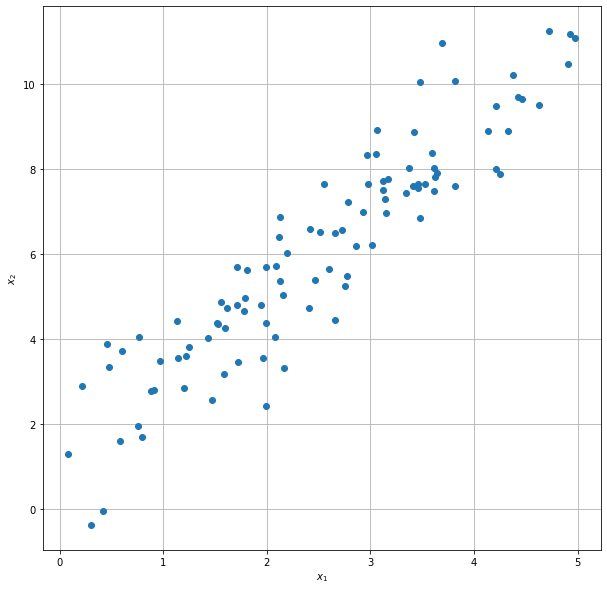
\includegraphics[width=0.45\linewidth]{figures/pca_dataset}
	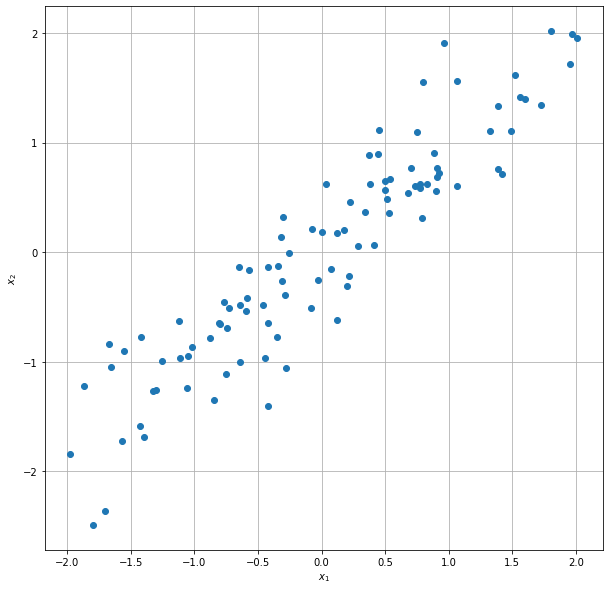
\includegraphics[width=0.45\linewidth]{figures/pca_dataset_centered}
	\caption{The dataset used in the PCA example (left), and the same dateset centered in the origin (right).}
	\label{fig:pca_dataset}
\end{figure}

\subsection{Covariance Matrix Computation}
The covariance matrix of our dataset helps us to understand if there is any relationship between the variables (i.e. sometimes, they are so correlated that they contain redundant information). So, in order to identify these correlations, we compute the covariance matrix.

The covariance matrix is a $n\times n$ (where $n$ is the number of dimensions) that has as entries the covariances associated with all possible pairs of the initial variables. Since the covariance of a variable with itself is its variance ($\textrm{cov}(a, a)= \textrm{var}(a)$), in the main diagonal (top-left to bottom-right) we actually have the variances of each initial variable. And since the covariance is commutative ($\textrm{cov}(a, b) = \textrm{cov}(b, a)$), the entries of the covariance matrix are symmetric with respect to diagonal.

Once we have centered our data around 0, $[X^T][X]$ is the covariance matrix.

\begin{equation}
[\Sigma]=[X^T][X] =
\begin{bmatrix}
\textrm{var}(x_1) & \textrm{cov}(x_2, x_1) & \cdots & \textrm{cov}(x_n, x_1) \\
\textrm{cov}(x_1, x_2) & \textrm{var}(x_2) & \cdots & \textrm{cov}(x_n, x_2) \\
\vdots & \vdots & \vdots & \vdots \\
\textrm{cov}(x_1, x_n) & \textrm{cov}(x_2, x_n) & \cdots & \textrm{var}(x_n)
\end{bmatrix}
\end{equation}

\subsection{Principal Components}

Principal components are new variables that are constructed as linear combinations or mixtures of the initial variables. These combinations are done in such a way that the new variables (i.e. principal components) are uncorrelated and most of the information within the initial variables is squeezed or compressed into the first components. 

So, the idea is that a $n$-dimensional dataset gives you $n$ principal components, but PCA tries to put maximum possible information in the first component, then maximum remaining information in the second and so on.

Organizing information in principal components this way, will allow you to reduce dimensionality without losing much information, and this by discarding the components with low information and considering the remaining components as your new variables.
%An important thing to realize here is that, the principal components are less interpretable and don’t have any real meaning since they are constructed as linear combinations of the initial variables.

Geometrically speaking, principal components represent the directions of the data that explain a maximal amount of variance, that is to say, the lines that capture most information of the data. The relationship between variance and information here, is that, the larger the variance carried by a line, the larger the dispersion of the data points along it, and the larger the dispersion along a line, the more the information it has.

It is possible to demonstrate that the eigenvectors of the covariance matrix are actually the directions of the axis where there is the most variance (i.e. most information) and that we call \emph{principal components}. Eigenvalues are simply the coefficients, attached to eigenvectors, which give the amount of variance carried in each principal component.

As we have seen in Sec.~\ref{find-eigenvalues-and-eigenvectors-in-python} the eigenvectors and eigenvalues of our dataset covariance are obtained as follows

\begin{ipython}
eigVals, eigVecs = np.linalg.eig(X_centered.T.dot(X_centered))
print (eigVecs)
\end{ipython}
\begin{ioutput}
[[-0.70710678 -0.70710678]
 [ 0.70710678 -0.70710678]]
\end{ioutput}

\begin{ipython}
print (eigVals)
\end{ipython}
\begin{ioutput}
[  7.46600865 192.53399135]
\end{ioutput}

If we rank the eigenvalues in descending order, we get $\lambda_2\gt\lambda_1$, which means that the eigenvector that corresponds to the first principal component (PC1) is  $v_2$ (i.e. the second column of the previous matrix).

After having the principal components, to compute the percentage of variance (information) accounted for by each component, we divide the eigenvalue of each component by the sum of eigenvalues. 

\begin{ipython}
for l in eigVals:
    print ("{:.1f}".format(l/np.sum(eigVals)*100))
\end{ipython}
\begin{ioutput}
3.7
96.3
\end{ioutput}

According to these results PC2 and PC1 carry respectively 96\% and 4\% of the variance of the data.

\subsection{Feature Vector}
Given the list of eigenvectors and eigenvalues we need to choose whether to keep all these components or discard those of lesser significance (i.e. of low eigenvalues), and form with the remaining ones a matrix called \emph{feature vector}.

So, the feature vector is simply a matrix that has as columns the eigenvectors of the components that we decide to keep. This makes it the first step towards dimensionality reduction, because if we choose to keep only $p$ eigenvectors (components) out of $n$, the final dataset will have only $p$ dimensions.

Continuing with the example from the previous step, we can either form a feature vector with both of the eigenvectors $v1$ and $v2$, or discard the eigenvector $v_2$, which is the one of lesser significance, and form a feature vector with $v_1$ only.

Discarding the eigenvector $v_1$ will reduce dimensionality by 1, and will consequently cause a loss of information in the final data set. But given that $v_1$ was carrying only 4\% of the information, the loss will be therefore not important and we will still have 96\% of the information that is carried by $v_2$.

Figure~\ref{fig:pca_result} shows the two principal components.

\begin{figure}[htb]
	\centering
	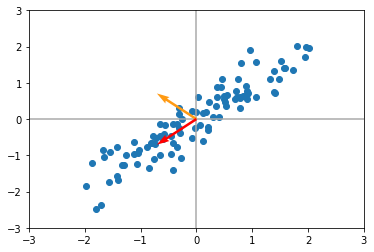
\includegraphics[width=0.7\linewidth]{figures/pca_result}
	\caption{The directions corresponding to the first two principal 
		components of our example dataset.}
	\label{fig:pca_result}
\end{figure}

\subsection{Recast Data Along Principal Components}
At this point we can use the feature vector to reorient data from the original axis to the ones represented by the principal components. 
This can be done by multiplying the transpose of the original dataset by the transpose of the feature vector

\begin{equation}
[Y] = [X^T][F^T]
\end{equation}

\begin{ipython}
Y = eigVecs.T.dot(X_centered.T)
\end{ipython}

The rotation transformed our dataset that have now the more variance on one of the basis axis (i.e. the Cartesian axis). 
You could keep only this dimension and have a fairly good representation of the data. Figure~\ref{fig:pca_rotated} shows the effect of such a rotation to our sample.
\clearpage
\begin{figure}[htb]
	\centering
	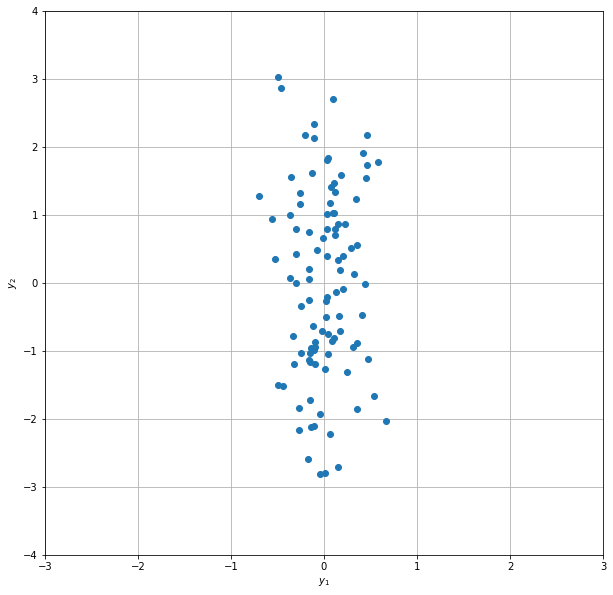
\includegraphics[width=0.5\linewidth]{figures/pca_rotated}
	\caption{The dataset rotated so that the usual Cartesian coordinates
		correspond to the first two principal components.}
	\label{fig:pca_rotated}
\end{figure}

\begin{thebibliography}{9}
\bibitem{bib:matrices}\href{https://algebra.nipissingu.ca/tutorials/matrices.html}{\emph{Matrices Tutorial}}, Nipissing University [Online]
\bibitem{bib:eigenvalues}\href{http://macosa.dima.unige.it/mat/calculus/eigenstuff.htm}{\emph{Eigenvectors and Eigenvalues}}, UniGe [Online]
\bibitem{bib:term_structure} D. Filipović, S. Willems, \emph{Exact Smooth Term-Structure Estimation}, arXiv:1606.03899, 2016
\bibitem{bib:pca} L. I. Smith, \href{http://www.iro.umontreal.ca/~pift6080/H09/documents/papers/pca_tutorial.pdf}{\emph{A tutorial on Principal Component Analysis}} [Online]
\end{thebibliography}







\chapter{Random Variables}
\label{fundamentals}

In this Chapter some basic concepts that will be used throughout the remaining part of these notes, are reviewed.

\section{Random Variable}
\label{random-variables}

In probability and statistics a random variable is described as a variable whose values depend on outcomes of a random phenomenon. 
%<<<<<<< HEAD:financial_markets_lectures/random_variables2.tex
%It can be formalized as a certain function that is defined over the set of all possible outcomes, referred to as sample space $\Omega$. 
%
%For example, in the event of a coin toss, only two outcomes are possible: heads or tails. If instead the random variable is designated to represent the sum of the resulting numbers after three dice are rolled, it could be 3 ($1 + 1+ 1$), 18 ($6 + 6 + 6$), or somewhere in between.
%
%In the corporate world, random variables can be assigned to properties such as the average price of an asset over a given time period, the return on investment after a specified number of years, the estimated turnover rate at a company within the following six months, etc. Risk analysts assign random variables to risk models when they want to estimate the probability of an adverse event occurring. 
%
%Since in all cases that are taken into account here, $X$ is real-valued, formally a random variable can be understood as a measurable function defined on a probability space that maps from the sample space to the real numbers.

The word "variable" in random variable is a misnomer since it is actually a function. And like all well behaved functions, a random variable, say $X$, has a domain and a range.

The domain $\Omega$ of $X$ is the sample space of random outcomes. These outcomes arise when some stochastic experiment is performed. The outcomes may or may not be numeric. 

For example, in the event of a coin toss, only two outcomes are possible: heads or tails. If instead the random variable is designated to represent the sum of the resulting numbers after three dice are rolled, it could be 3 ($1 + 1+ 1$), 18 ($6 + 6 + 6$), or somewhere in between.

In the corporate world, random variables can be assigned to properties such as the average price of an asset over a given time period, the return on investment after a specified number of years, the estimated turnover rate at a company within the following six months\ldots Risk analysts assign random variables to risk models when they want to estimate the probability of an adverse event occurring. 

%It can be formalized as a certain function that is defined over the set of all possible outcomes, referred to as sample space $\Omega$. 

Since in all cases that are taken into account here, $X$ is real-valued, formally a random variable can be understood as a measurable function defined on a probability space that maps from the sample space to the real numbers, i.e. the range.

%\begin{equation}
%X:\Omega \rightarrow E
%\end{equation}
%where $E=\mathbb {R}$, or in words, $E$ represents the set of real numbers. 

Random variable's values might represent the possible outcomes of a yet-to-be-performed experiment. They may also conceptually represent either the results of an "objectively" random process (such as rolling a die). As a function, a random variable is required to be measurable, which allows for probabilities to be assigned to its potential values. 

A random variable is different from an algebraic one. An equation variable is an unknown value that can be calculated. The equation $10 + x = 13$ shows that we can calculate the specific value for $x$ which is 3. On the other hand, a random variable has a set of values, and any of those values could be the resulting outcome.

When the range of possible values for $X$ is unaccountably infinite then $X$ is called a \emph{continuous random variable} and its distribution can be described by a \emph{probability density function} (PDF). Contrary if the range is countable, the random variable is called a \emph{discrete random variable} and its distribution can be interpreted as a discrete probability distribution.

The PDF is used to specify the probability of the random variable falling within a particular range of values. By definition 
the probability density function is non-negative everywhere, and its integral over the entire space is equal to 1.
Left plot in Fig.~\ref{fig:pdf_pmf} shows an example of Gaussian probability density function.

Why then is $X$ called a random variable? It’s because $X$ outputs values using a probability distribution that is supposed to represent the likelihoods of occurrences of events in the sample space. 

%A random variable is different from an algebraic one. An equation variable is an unknown value that can be calculated. The equation $10 + x = 13$ shows that we can calculate the specific value for $x$ which is 3. On the other hand, a random variable has a set of values, and any of those values could be the resulting outcome.

When the range of possible values for $X$ is unaccountably-countably infinite then $X$ is called a \emph{continuous random variable} and its distribution can be described by a \emph{probability density function} (PDF). Contrary if the range is countable, the random variable is called a \emph{discrete random variable} and its distribution can be interpreted as a discrete probability distribution.

The PDF is used to specify the probability of the random variable falling within a particular range of values. By definition 
the probability density function is non-negative everywhere, and its integral over the entire space is equal to 1.
Left plot in Fig.~\ref{fig:pdf_pmf} shows an example of Gaussian probability density function.

%<<<<<<< HEAD
%=======
%>>>>>>> a1ac7f24ce4566e11029c1fa992020cf704cc565:financial_markets_lectures/random_variables.tex
%>>>>>>> a1ac7f24ce4566e11029c1fa992020cf704cc565
In the context of discrete random variables the probability density function is usually referred to as \emph{probability mass function} (PMF). Right plot in Fig.~\ref{fig:pdf_pmf} shows an example of discrete probability density function.

\begin{figure}[htb]
	\centering
	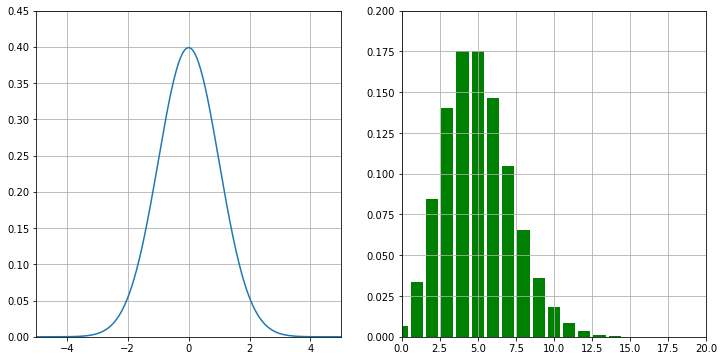
\includegraphics[width=1.\textwidth]{figures/pdf_pmf.png}
	\caption{On the left an example of continuous probability density function (Normal), on the right a discrete probability mass function (Poissonian).}
	\label{fig:pdf_pmf}
\end{figure}

\subsection{Cumulative Distribution and Quantile Functions}
\label{sec:quantile-function}

The \emph{cumulative distribution function} (CDF) $F$ of a random variable $X$, evaluated at $x$, gives the probability that $X$ will take a value less than or equal to $x$

\begin{equation}
F_X(x) = P(X \le x)\qquad\mathrm{or~equivalently}~\int_{-\infty}^{x}{f(X)dX}
\end{equation}
so it gives the area under the probability density function $f$ from minus infinity to $x$.
The probability that $X$ lies in the interval $(a,b]$ is therefore

\begin{equation}
P(a> X \le b)=F_{X}(b)-F_{X}(a)\qquad\mathrm{or}~\int_a^b{f(X)dX}
\end{equation}
Notice that by the previous definition any random variable can be conveniently described by its cumulative distribution too.

The \emph{quantile function} $Q$, associated with a probability distribution of a random variable, specifies the value $x$ of the random variable such that the probability $p$ of the variable being less than or equal to that value equals the given probability. It is also called the percent-point function (PPF) or inverse cumulative distribution.

In terms of the cumulative distribution function $F$, the quantile function $Q$ returns the value $x_p$ such that 

\begin{equation}
F_{X}(x_p)=P(X\le x_p)=p
\end{equation}
So the quantile function can be considered the "inverse" of the cumulative distribution function: given a probability $p$ (or a value of the CDF) it returns the $x$ at which the CDF reaches this probability, so we can write $Q=F^{-1}$.

In Fig.~\ref{fig:percentile} an example related to the Gaussian distribution is shown. On the left side the Gaussian PDF is drawn, the red area represents the 30\% of the total area (which is 1 by definition). On the right the corresponding CDF is plotted, the point at which the CDF reaches 30\% is highlighted. The corresponding quantile value is also indicated and is $-0.5244$.

\begin{figure}[htb]
	\centering
	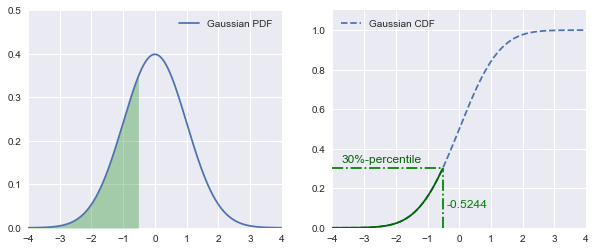
\includegraphics[width=1.\textwidth]{figures/percentile.png}
	\caption{On the left a standard normal distribution, the filled region represent the 30\% of the total area under the curve. On the right the corresponding CDF with the 30\% point and the relative quantile highlighted.}
	\label{fig:percentile}
\end{figure}

The computation of CDF and quantiles is quite simple in \texttt{python}. The implementation of many distributions is available in \texttt{scipy.stats} module and for each of them the methods \texttt{cdf(x)} and \texttt{ppf(x)} can be used to evaluate CDF and quantile respectively.

\begin{ipython}
from scipy.stats import norm

quantile = norm.ppf(0.3)
cdf = norm.cdf(quantile)
print (f"30%-quantile of standard normal is {quantile}")
print (f"CDF value at {quantile}: {cdf}")
\end{ipython}
\begin{ioutput}
30%-quantile of standard normal is -0.5244005127080409
CDF value at -0.5244005127080409: 0.29999999999999993
\end{ioutput}

If instead of a distribution a dataset is involved, the quantile can be determined using the function \texttt{numpy.percentile} (e.g. this will be useful when estimating VaR). Notice that in this case we are talking about \emph{percentile} which is the \emph{quantile} times 100 (e.g. 50-percentile is equivalent to 0.5-quantile).

\begin{ipython}
import numpy
dist = [1, 2, 3, 4, 5, 6, 7, 8, 9]

# first argument the data-set
# second argument a list of percentiles
perc = numpy.percentile(dist, [1, 50])
print (perc)
\end{ipython}
\begin{ioutput}
[1.08 5.  ]
\end{ioutput}

\subsection{Expected Value}\label{sec:expected-value}

Since a random variable is connected to a probabilistic event, it is necessary to take into account all the possible values it can take for its evaluation. This is done with the \emph{expected value}
which is a generalization of the weighted average, and is intuitively the arithmetic mean of all the possible realizations of a random variable \(X\).

\subsubsection{Discrete Case}
Consider a random variable with a finite number of outcomes $(x_{1},x_{2},\ldots ,x_{k})$ occurring with probabilities $(p_{1},p_{2},\ldots ,p_{k})$ respectively. The expectation of $X$ is then defined as

\begin{equation}
	\mathbb{E}[X]=\sum _{i=1}^{k}x_{i}\,p_{i}=x_{1}p_{1}+x_{2}p_{2}+\cdots +x_{k}p_{k}
\end{equation}

Since $p_{1}+p_{2}+\cdots +p_{k}=1$, the expected value is the average of the $x_{i}$ weighted by their probabilities $p_{i}$.

%By definition, the expected value of a constant random variable \(X=c\) equals its constant value \(c\). Instead the expected value of a random variable \(X\) with equiprobable outcomes \((c_{1},\ldots ,c_{n})\) is defined as the arithmetic mean of the terms \(c_i\). 

As an example let $X$ represent the outcome of a single roll of a fair six-sided die. The possible values for $X$ are 1, 2, 3, 4, 5, and 6, all of which are equally likely with probability $1/6$.

The expectation of $X$ is then

\begin{equation*}
	\mathbb{E}[X]=1\cdot {\frac {1}{6}}+2\cdot {\frac {1}{6}}+3\cdot {\frac {1}{6}}+4\cdot {\frac {1}{6}}+5\cdot {\frac {1}{6}}+6\cdot {\frac {1}{6}}=3.5
\end{equation*}
If one rolls the die $n$ times and computes the results average, then as $n$ grows, this average converges to the expected value.

\subsubsection{Continuous Case}
If $X$ is a random variable with a probability density function, $f(x)$, then the expected value is defined as

\begin{equation}
\mathbb{E}[X]=\int_{\Omega}xf(x)dx
\end{equation}
For multidimensional random variables, the expected value is defined per component, that is,

\begin{equation}
\mathbb{E}[(X_{1},\ldots ,X_{n})]=(\mathbb{E} [X_{1}],\ldots ,\mathbb{E}[X_{n}])
\end{equation}

\subsection{Some Properties of Expected Value}
\label{some-properties}

\begin{itemize}
\tightlist
\item Let $\mathbb{1}_{A}$ denote the indicator function of an event $A$ (i.e. a function whose value is 1 if the event $A$ happens, 0 otherwise), then

\begin{equation}
\mathbb{E}[\mathbb{1}_{A}] = 1\cdot P(A)+0\cdot P(\Omega \setminus A)= P(A)
\end{equation}

\item the expected value operator \(\mathbb{E}\) is linear in the sense that, for any random variables $X$ and $Y$, and a constant $a$
\begin{equation}
\begin{cases}
\mathbb{E}[X+Y] = \mathbb{E}[X] + \mathbb{E}[Y] \\
\mathbb{E}[aX] = a\mathbb{E}[X]
\end{cases}
\end{equation}

This means that the expected value of the sum of any finite number of random variables is the sum of the expected values of the individual random variables, and the expected value scales linearly with a multiplicative constant;

\item the expected value of a measurable function of $X$, $g(X)$, given that $X$ has a probability density function $f(x)$, is given by 

\begin{equation}
\mathbb{E}[g(X)] = \int_{\Omega}g(x)f(x) dx
\end{equation}

This formula also holds in multidimensional case, when $g$ is a function of several random variables, and $f$ is their joint density;

\item $n$ random variables $X_1 ,\ldots , X_n$ are independent if the following property holds for all positive functions $f_1 ,\ldots , f_n$

\begin{equation}
\mathbb{E}[f_1 (X_1 )\cdots f_n (X_n )] = \mathbb{E}[f_1 ( X_1 )] \cdots \mathbb{E}[f_n (X_n )]
\end{equation}
\end{itemize}


%
%We have seen so far how to generate a sequence of random numbers from U
%{[}0, 1{]}. However, most of the simulations include the sampling of
%random variables, or even random vectors in a mul- tidimensional case,
%from specified, not uniform distributions. Sampling of nonuniform random
%variates is done indirectly, i.e.~one transforms samples from the
%uniform to a desired nonuniform distribution. Accordingly, each
%realization of a nonuniform random variable is directly obtained from a
%single uniform variate or from a sequence of uniforms {[}46, p.54{]}.
%There are numerous algorithms that allow you to generate random numbers
%from a certain desired distribution. However, two main criteria in order
%to choose between them are accuracy and speed.


%
%\hypertarget{correlated-normal-variables-and-vectors}{%
%\subsubsection{Correlated normal variables and
%	vectors}\label{correlated-normal-variables-and-vectors}}
%
%A \(d\)-variate normal distribution \(\phi(\mu, \Sigma)\) is generally
%specified by its mean vector \(\mu\) and variance- covariance matrix
%\(\Sigma\). Random vectors from a multivariate normal distribution can
%be generated directly by generating a \(d\)-vector of iid standard
%normal deviates \(z' = (z_1 , z_2 ,\dots , z_d)\).
%
%Next we know from the linear transformation property that if the vector
%\(z∼\phi_d (0,I)\) and \(x = \mu + Az\), then \(x ∼\phi_d (\mu, AA')\).
%Therefore, we can generate a sequence of univariate normal random
%variables \(z_i\) and put them into a vector \(z\). Thus the challenge
%is merely made up of finding the matrix \(A\) for which the property
%\(AA' = \Sigma\) holds. The representation of \(\Sigma\) as \(AA'\) with
%\(A\) as a lower triangular matrix is denoted as a Cholesky
%factorization of the variance-covariance matrix \(\Sigma\). If
%\(\Sigma\) is symmetric positive definite there is a Cholesky
%factorization and the sampling of multivariate normals is easily done by
%basically sampling from a univariate \(\phi(0,1)\).
%
%In some applications in finance random variables or vectors are required
%to depend on each other in a prescribed way, i.e.~they must not be
%totally uncorrelated. Correlated random variables are calculated
%according to the following algorithm:
%
%\begin{enumerate}
%\def\labelenumi{\arabic{enumi}.}
%\tightlist
%\item
%calculate the Cholesky factorization \(AA′ = \Sigma\),
%\item
%calculate \(z ∼ \phi(0,I)\) by component, for \(i = 1,2,\ldots ,d\),
%\item
%\(x=\mu + Az\), then \(x∼\phi (\mu, \Sigma )\).
%\end{enumerate}
%
%Suppose we have a two-dimensional case, \(d = 2\). Next we are looking
%for a vector \(x' = (x_1 , x_2 ) ∼ \phi (0, \Sigma )\). The correlation
%between \(x_1\) and \(x_2\) is denoted by \(\rho\) and thus the Cholesky
%factorization provides \(\Sigma = AA'\)
%
%\[\begin{bmatrix}
%\sigma_1^2 & \rho\sigma_1 \sigma_2\\
%\rho\sigma_1 \sigma_2 & \sigma_2^2 
%\end{bmatrix} = 
%\begin{bmatrix}
%\sigma_1 & 0\\
%\rho\sigma_2 & \sigma_2\sqrt{1-\rho^2} 
%\end{bmatrix}
%\begin{bmatrix}
%\sigma_1 & \rho\sigma_2 \\
%0 & \sigma_2\sqrt{1-\rho^2} 
%\end{bmatrix}\]
%
%If \(z_1\) and \(z_2\) are independent and from \(\phi(0, 1)\), then
%
%\[\begin{bmatrix}
%x_1\\
%x_2 
%\end{bmatrix} = A
%\begin{bmatrix}
%z_1\\
%z_2 
%\end{bmatrix} = 
%\begin{bmatrix}
%\sigma_1 z_1\\
%\sigma_2 (\rho z_1 + \sqrt{1-\rho^2}z_2) 
%\end{bmatrix}
%\]
%
%are distributed according to \(\phi(0, \Sigma)\).
%
%\begin{codebox}
%\prompt{In}{incolor}{ }{\boxspacing}
%\begin{Verbatim}[commandchars=\\\{\}]
%	
%\end{Verbatim}
%\end{codebox}

\section*{Exercises}
\begin{question}
A random variable $X$ that assumes values in the interval $[0, 1]$ has density function $f(x) = a + b x$,
where $a$ and $b$ are two constants to be determined.

\begin{enumerate}[label={\emph{\alph*})}]
\tightlist
\item Compute $a$ and $b$ such that $f(x)$ has a PDF with probability density in $X = 1$ being the double of the probability density in $X = 0$;
\item compute the quartiles (0.25, 0.5, 0.75 quantiles) of the random variable $X$.
\end{enumerate}
\end{question}

\begin{solution}
\begin{enumerate}[label={\emph{\alph*})}]
\tightlist
\item Given the PDF of the random variable $f(x) = a + bx$ the two constants $a$ and $b$ can be determined by imposing the normalization of the density function and the required conditions at the boundaries:

\begin{equation*}
\begin{cases}
f(1) = 2\cdot f(0)\\
\int_0^1 f(x)dx = 1
\end{cases}  
\end{equation*}
The first equation gives $a+b = 2a \implies a = b$ while the integral can be easily solved

\begin{equation*}
\int_0^1 f(x)dx = \left(ax + \frac{a}{2}x^2\right|^1_0 = 1 \implies a = \frac{2}{3}
\end{equation*}

\item From the first point we fully determined the PDF $f(x) = \frac{2}{3}(1 + x)$. To compute the quartiles it is first necessary to integrate it to get the corresponding CDF 
\begin{equation*}
F(x) = \int_0^{1/4} f(x)dx = \frac{2}{3}\left(x + \frac{1}{2}x^2\right) = \frac{1}{3}x^2 + \frac{2}{3} x  - \frac{1}{4}
\end{equation*}

Then the first quartile ($Q_1$) is given by $F^{-1}(x) = 1/4$ and similarly for the others
\begin{gather*}
\frac{1}{3}x^2 + \frac{2}{3} x  = \frac{1}{4} \\
Q_1 = -1 \pm \frac{3}{2}\sqrt{\frac{7}{9}} = \frac{1}{2}(\sqrt{7} - 2) = 0.3229\\
Q_2 = \dots = 0.5811\\
Q_3 = \dots = 0.8028
\end{gather*}
\end{enumerate}
\end{solution}

\begin{question}
\label{ex:greedy_pig}
The Greedy Pig Game is a simple dice game. It is played with one single die and the goal is to reach 100 points. Each player in turn starts to roll the die, if it results to be in [2, 6] the corresponding points are acquired and the player can decide either to continue to roll or to stop. If a 1 is rolled the player scores a 0 and her turn ends.

\begin{itemize}
\item What is the expected number of points for one roll ?
\item Imagine a player that has collected $k$ points. Compute and draw the expected points obtained with a further roll. What can be concluded from this plot ?
\end{itemize}
\end{question}

\cprotEnv\begin{solution}
The expected number of points for one roll is the weighted average of the possible points [2, 6] (when the die is 1 no points are assigned) with the probability of 1/6.
\begin{ipython}
ex_roll = 0
for i in range(2, 7):
    ex_roll += 1/6*i

print (ex_roll)
\end{ipython}
\begin{ioutput}
3.3333333333333
\end{ioutput}

If the current points of a player are $k$, in computing the expectation, beside the [2, 6]*1/6 terms, it has to be added a $-k\cdot 1/6$ term in case a 1 is rolled (i.e. in this case the total score goes to 0 and the turn ends).
\begin{ipython}
from matplotlib import pyplot as plt

exps = []
for k in range(1, 51):
    exp = -k*1/6
    for i in range(2, 7):
        exp += 1/6*i
    exps.append(exp)

fig = plt.figure(figsize=(10,8))
plt.plot(range(1, 51), exps)
plt.grid(True)
plt.xlabel("current turn points ($k$)")
plt.ylabel("expected points next roll")
plt.show()
\end{ipython}

Figure~\ref{fig:greedy_pig_expec} shows the expected points distribution in the next roll as a function of the current player points. It looks like that when the player has more than 20 points the expectation becomes negative, so it is not anymore convenient to keep rolling. This is a fundamental clue to derive a game strategy: \emph{keeps rolling until you reach 20 points}.

\begin{figure}[htbp]
	\begin{center}
		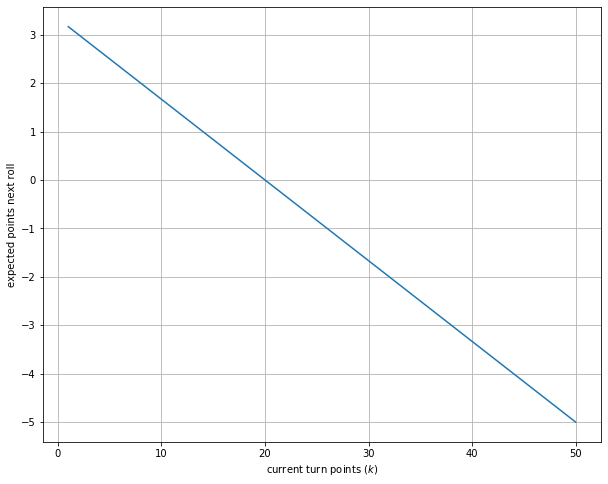
\includegraphics[width=0.7\linewidth]{figures/greedy_pig_expectation}
	\end{center}
\caption{Expected points in the next roll as a function of the current turn points.}
\label{fig:greedy_pig_expec}
\end{figure}
\end{solution}

\begin{question}
Let $X$ be a random variable with density function

\begin{equation*}
f(x) = 
\begin{cases}
k(1 - x^2),~\textrm{if}~0 \leq x \leq 1\\
0,~\textrm{otherwise}		
\end{cases}
\end{equation*}
Find $k$, together with the expectation and the variance of the random variable $Y$ defined as $Y = 3X - 1$.
\end{question}

\cprotEnv\begin{solution}
\label{ex:variance}
To find the value of $k$ we can exploit the normalization condition for a probability density:

\begin{equation*}
\begin{gathered}
\int_\Omega f(x) d\Omega = 1\\
\int_{0}^{1}k(1-x^{2})dx = k\left(x-\frac{1}{3}x^{3}\right|_{0}^{1}= k\left(1-\frac{1}{3}\right) \\
k\left(1-\frac{1}{3}\right) = 1 \implies k = \frac{3}{2}
\end{gathered}
\end{equation*}

The expectation of the variable $Y$ instead equals to
\begin{equation*}
\mathbb{E}[Y] = 3\mathbb{E}[X] - 1
\end{equation*}	
So
\begin{equation*}
\begin{gathered}
\mathbb{E}[X] = \frac{3}{2}\int_{0}^{1}x(1-x^2)dx = \frac{3}{2}\left(\frac{1}{2}x^2-\frac{1}{4}x^{4}\right|_{0}^{1} = \frac{3}{2}\left(\frac{1}{2}-\frac{1}{4}\right) = \frac{3}{8} \\
\mathbb{E}[Y] = 3\cdot\frac{3}{8} - 1 = \frac{1}{8} 
\end{gathered}
\end{equation*}
And finally for the variance:
\begin{equation*}
\begin{aligned}
Var[Y] = & \mathbb{E}[Y^2] - (\mathbb{E}[Y])^2 = \frac{3}{2}\int_{0}^{1}(9x^2 - 6x + 1)(1-x^2)dx - \frac{1}{64} = \\  &\frac{3}{2}\int_{0}^{1}(- 9x^4 + 6x^3 + 8x^2 - 6x + 1)dx - \frac{1}{64} = 
\frac{3}{2}\left(- \frac{9}{5}x^5 + \frac{6}{4}x^4 + \frac{8}{3}x^3 - 3x^2 + x\right|_{0}^{1} - \frac{1}{64} = \\
& \frac{3}{2}\left(- \frac{9}{5} + \frac{6}{4} + \frac{8}{3} - 3 + 1\right) - \frac{1}{64} = \frac{11}{20} - \frac{1}{64} = \frac{171}{320}
\end{aligned}
\end{equation*}

Alternatively it can be demonstrated that the variance of a random variable $Y = a + bX$ can be computed as $Var[Y] = b^2 Var[X]$. Indeed starting from the general form of the variance $Var[Y] = \mathbb{E}[Y^2] - (\mathbb{E}[Y])^2$ and computing each term of the right hand side of the equation 

\begin{equation}
\begin{gathered}
\mathbb{E}[Y^2] = \mathbb{E}[(a+bX)^2] = \mathbb{E}[b^2X^2 + 2abX + a^2] = b^2\mathbb{E}[X^2] + 2ab\mathbb{E}[X]+ a^2  \\
\mathbb{E}[Y]^2 =  (b\mathbb{E}[X] + a)^2 = b^2\mathbb{E}[X]^2 + 2ab\mathbb{E}[X]+ a^2  
\label{eq:each_var}
\end{gathered}
\end{equation}
Substituting Eqs.~\ref{eq:each_var} into the general form of the variance 
\begin{equation}
\begin{gathered}
Var[Y] = b^2\mathbb{E}[X^2] + 2ab\mathbb{E}[X]+ a^2 - (b^2\mathbb{E}[X]^2 + 2ab\mathbb{E}[X]+ a^2) \\ 
= b^2\mathbb{E}[X^2] - b^2\mathbb{E}[X]^2 = b^2 Var[X]
\end{gathered}     
\end{equation}

So $Var[Y] = 9\mathbb{E}[X]$.
\end{solution}

\begin{question}
We want to insure a car of 12000 EUR. The probability that a car is involved in an accident during a year is 0.15 in which case the amount of damage is

\begin{itemize}
\tightlist
\item 20\% of its value with probability 0.8;
\item 60\% of its value with probability 0.12;
\item 100\% of its value with probability 0.08.
\end{itemize}
Find the first annual premium the insurer must charge to have the expected cost of the company equal to 0.
\end{question}

\cprotEnv\begin{solution}
\begin{ipython}
print (f"{0.15 * 12000 * (0.8*0.2 + 0.6*0.12 + 0.08):.2f} EUR")
\end{ipython}
\begin{ioutput}
561.60 EUR
\end{ioutput}
\end{solution}

\begin{question}
The daily expenditure ($X$, in euros) spent by a certain customer in a department store is distributed according to the following density function:

\begin{equation*}
f(x) = 
\begin{cases}
x^2/9000,~\textrm{if}~0 \leq x \leq 30\\
0,~\textrm{otherwise}		
\end{cases}
\end{equation*}

\begin{enumerate}[label={\emph{\alph*})}]
\item calculate the probability that the client has a daily spending between 15 and 20 EUR;
\item what is his/her expected daily expenditure ?;
\item next winter the department store is granting the following "discount vouchers", whose amount depends on the client's expenditure: 1 EUR for spending between 10 and 20 EUR, 1.5 EUR for spending between 20 and 25 EUR,
3 EUR if the expense exceeds 25 EUR. Derive the distribution and the expected value of the discounts obtained by the client.
\item the customer has paid for his/her purchases in the store with a credit card which applies a 4\% charge. What is the probability that the customer has paid (with charges included) between 10 and 15 EUR ?
\end{enumerate}
\end{question}

\cprotEnv\begin{solution}
\begin{enumerate}[label={\emph{\alph*})}]
\tightlist
\item First we need to calculate the CDF by simple integration of the given PDF.
\begin{ipython}
def F(x):
    return x**3/27000

P = F(20) - F(15)
print (P)
\end{ipython}
\begin{ioutput}
0.17129629629629628
\end{ioutput}
\item The expected expense is given by $\int_{0}^{30} xf(x) dx = x^4/36000$
\begin{ipython}
def tot(x):
    return x**4/36000

print (tot(30))
\end{ipython}
\begin{ioutput}
22.5	
\end{ioutput}

\item The expected discount value is given by the weighted average of each discount times the probability of spending the corresponding amount of money:
\begin{ipython}
expected = 1 * (F(20)-F(10)) + 1.5 * (F(25) - F(20)) + 3 * (F(30) - F(25))
print (expected)
\end{ipython}
\begin{ioutput}
1.9467592592592593
\end{ioutput}

\item If the customer spent between 10 and 15 EUR with an extra charge of 4\% (by the usage of the credit card) the real expense limits has to be scaled by $1 - 0.04$, then the corresponding probability can be found using the function \texttt{F}:
\begin{ipython}
xmin = 10*0.96
xmax = 15*0.96
P = F(xmax) - F(xmin)

print (P)
\end{ipython}
\begin{ioutput}
0.07782399999999998
\end{ioutput}
\end{enumerate}
\end{solution}

\cprotEnv\begin{question}
An economist wishes to estimate the total cost of a project. His salary is composed of a fixed part of 12000 EUR plus a variable part of 300 EUR per day of work. The project can be performed between 7 and 11 days, and the economist has derived the following subjective probability distribution for the random variable $X$ (number of days it will take to implement the project):
\begin{ipython}
P = {7:0.10, 8:0.20, 9:?, 10:0.30, 11:0.10}
\end{ipython}
\begin{enumerate}[label={\emph{\alph*})}]
\tightlist
\item What is the probability that the project is carried out in 9 days? Justify your answer.
\item Determine the expected cost of the project and its variance. 
\end{enumerate}
\end{question}

\cprotEnv\begin{solution}
\begin{enumerate}[label={\emph{\alph*})}]
\tightlist
\item Since the assumption is that the work can be completed in between 7 and 11 days, the sum of $P$s has to equal 1. So $P(9)$ can be determined as
\begin{ipython}
P = {7:0.10, 8:0.20, 10:0.30, 11:0.10}
P[9] = 1 - (P[7]+P[8]+P[9]+P[10]+P[11])

print (f"{P[9]:.2f}")
\end{ipython}
\begin{ioutput}
0.30
\end{ioutput}
\item The expected cost of the project results
\begin{ipython}
expected_days = sum([d*p for d, k in P.items()])
E_C = 12000 + 300*expected_days

print (E_C)
\end{ipython}
\begin{ioutput}
14730.0	
\end{ioutput}

Remembering Solution~\ref{ex:variance} the variance in the costs $Var[C]$ (which follows a linear relationship with the number of days $C = 12000 + 300\cdot d$) becomes
\begin{ipython}
var_days = sum([(d**2)*p for d, k in P.items()])
b = 300
print (b**2 * var_days)
\end{ipython}
\begin{ioutput}
116100.0	
\end{ioutput}
\end{enumerate}
\end{solution}

\begin{question}
A casino advertises that the expected prize won by its clients is 600 EUR, with risk $\sigma$ = 360.
\begin{enumerate}[label={\emph{\alph*})}]
\tightlist
\item Calculate the probability that a player wins between 150 and 1050 EUR.
\item How would the above probability change if $\sigma$ = 420 ?
\item What is the probability that the prize won by a player deviates at least 504 EUR from its expectation?
\end{enumerate}
\end{question}

\cprotEnv\begin{solution}
In this case it is safe to assume that the wins are distributed as a Gaussian with mean 600 EUR and standard deviation 360 EUR. 
\begin{enumerate}[label={\emph{\alph*})}]
\tightlist
\item It is much easier to convert the initial distribution to a standard normal (zero mean and unit variance) using the following transformation
\begin{equation*}
x' = \frac{(x - \mu)}{\sigma}
\end{equation*}
in such a way \texttt{scipy.stats.norm} can be used.

\begin{ipython}
from scipy.stats import norm

# convert the two limits in the standard normal
xmin = (150 - 600)/360
xmax = (1050 - 600)/360

print (xmin, xmax)
print (norm.cdf(xmax) - norm.cdf(xmin))
\end{ipython}
\begin{ioutput}
-1.25 1.25
0.7887004526662893
\end{ioutput}

\item If the risk (i.e. uncertainty) increases the probability of winning an amount of money in the same range is expected to decrease. Let's check using the same technique as in the previous answer.
\begin{ipython}
xmin = (150 - 600)/420
xmax = (1050 - 600)/420

print (xmin, xmax)
print (norm.cdf(xmax) - norm.cdf(xmin))
\end{ipython}
\begin{ioutput}
-1.0714285714285714 1.0714285714285714
0.7160232282490884
\end{ioutput}

Indeed now the range has shrunk from $\pm1.5\sigma$ to $\pm1.07\sigma$. 

\item Finally, we can determine the probability that a win exceeds 504 EUR the mean in a similar fashion.

\begin{ipython}
xmin = 504/360

print (xmin)
# the factor 2 because the win can exceed both ways the mean
print (norm.cdf(-xmin) * 2)
\end{ipython}
\begin{ioutput}
1.4
0.16151331846754213
\end{ioutput}
\end{enumerate}
\end{solution}


\begin{thebibliography}{9}
\bibitem{bib:random_variable}\href{http://www.stat.yale.edu/Courses/1997-98/101/ranvar.htm}{\emph{Random Variables}}, Yale University [Online]
\bibitem{bib:pdf} \href{https://mathinsight.org/probability_density_function_idea}{\emph{The idea of a probability density function}} [Online]
\bibitem{bib:cdf}\href{https://www.probabilitycourse.com/chapter3/3_2_1_cdf.php}{\emph{Cumulative Distribution Function }}, Probability Course [Online]
\bibitem{bib:quantile}\href{https://en.wikipedia.org/wiki/Quantile}{\emph{Quantile}}, Wikipedia [Online]
\bibitem{bib:expected_value}\href{https://www.investopedia.com/terms/e/expected-value.asp}{\emph{Expected Value}}, Investopedia [Online]
\end{thebibliography}
\chapter{Interpolation, Discount Factors and Forward Rates}
\label{interpolation}

In this Chapter we will begin to see some \texttt{python} applications to financial calculations, in particular discount curves and forward rates will be involved. In doing so we will review a widely used mathematical tool: \emph{interpolation}.

\section{Discounting}
\label{discount-factors}

%\subsection{Time Value of Money}
%Imagine a bank that offers a guaranteed return of 10\% on whichever amount of money a client put in her account as long as that amount stays in the account for one full year (no withdrawals possible). If the client knows would need \$11000 at the end of one year, how much money does she need to put in today so that the $X$ amount (principal) at the claimed 10\% a year interest rate will grow to the desired amount ?
%
%We know that at 10\% $X$ dollar today grows to
%
%\begin{equation}
%X * (1 + 0.1) = Y
%\end{equation}
%in one year, so the needed investment $X$ can be found by inverting the previous formula:
%
%\begin{equation*}
%X \cdot (1 + 10\%) = 11000 \implies X = \cfrac{11000}{(1 + 10\%)}
%\end{equation*}
%
%\begin{ipython}
%11000 / (1 + 0.1)
%\end{ipython}
%\begin{ioutput}
%10000
%\end{ioutput}
%
%What this says is that to have \$11000 in one year from now, the client needs to invest \$10000.
%What about 11000 dollars in two years from now ? Taking the approach used above
%
%\begin{equation*}
%	X = \cfrac{11000}{\left((1 + 10\%) \cdot (1 + 10\%)\right)} =  \cfrac{11000}{(1+10\%)^ 2}
%\end{equation*}
%
%\begin{ipython}
%11000 / (1 + 0.1)**2
%\end{ipython}
%\begin{ioutput}
%9090.90909090909
%\end{ioutput}
%
%In other words this means the \$11000 we need in two years from now are valued about 9090 dollars today.
%
%What we have just done above is called \emph{discounting}. We are adjusting a future value to bring it to its present value (PV or NPV). The rate used to adjust the future payment is called the \emph{discount rate}.
%
%The idea behind discounting is also known as \emph{time value of money}. Since a dollar will grow in any bank account at that certain rate, if it is invested in an alternative opportunity, it should at least earn that same rate to even consider the alternative worth thinking about. 
%The bottom line is that if you fail to earn the discount rate, you have actually lost money, anything less than that would mean you have not put your money to its best use.
%
%When we calculate the value of future payments today, we are doing a present value calculation. When we calculate the value of anything in the future we do a \emph{future value} calculation.
%
%A positive NPV denotes that at a certain cost of capital the returns or inflows from an investment opportunity outweigh the outflows and vice-versa. Obviously, when comparing various alternatives available for investment, the option with the most positive NPV or least negative NPV will be favoured. 
%
%As an example imagine that you have the chance to invest in a project, that will pay \$100 in year 1, and \$200 in year 2. How much are you willing to pay for this opportunity ? (assume an annual discount rate of 10\%).
%
%The answer is that you will be willing to pay at most an amount that is equal to the present value of this payments stream. To calculate it you need to scale each payment by its respective discount factors ($D(0, T)$ discount factor for year $T$)
%\begin{equation}
%D(0, T) = \cfrac{1}{(1 + r)^T}
%\label{eq:discount_factor}
%\end{equation}
%
%\begin{ipython}
%d1 = 1/(1 + 0.1)**1
%d2 = 1/(1 + 0.1)**2
%
%print ("discount factor for year 1: {:.2f}".format(d1))
%print ("discount factor for year 2: {:.2f}".format(d2))
%
%pv = 100*d1 + 200*d2
%
%print ("Total PV: {:.2f}".format(pv))
%\end{ipython}
%\begin{ioutput}
%discount factor for year 1: 0.91
%discount factor for year 2: 0.83
%Total PV: 256.20
%\end{ioutput}
%\noindent
%Hence, you would be willing to pay \$256.2 for this opportunity.
%
%%If there are $Y$ payments each year the discount factor formula becomes
%%
%%\begin{equation}
%%D(0, T) = \left(1+\cfrac{r}{Y}\right)^{-T}
%%\end{equation}
%%\noindent
%When the continuously-compounded hypothesis is used the discount factor becomes
%
%\begin{equation}
%D(0, T) = e^{-rT}
%\end{equation}

\section{Linear Interpolation}
\label{linear-interpolation}

Consider to have few data points, obtained by sampling or experimenting. These points represent the values of a not well known function $f(x)$, where $x$ is an independent variable (e.g. in recording a trip: distances at certain times, $d = f(t)$).

It may be necessary to estimate values of the function $f$ at particular $x$ for which samples are not available. Interpolation is a method of "constructing" these "new points" within the range of known data.

Let's clarify the technique with an example.
Assume you are going on holiday by car and that luckily there isn't much traffic so that you can drive at constant speed (which gives a linear relation between traveled space and time i.e.~$s = v \cdot t$. This means that if you plot the distances $s$ as a function of the time $t$ you get a line with slope $v$), see Fig.~\ref{fig:samples_for_interpolation}.

\begin{figure}[hb]
  \centering
  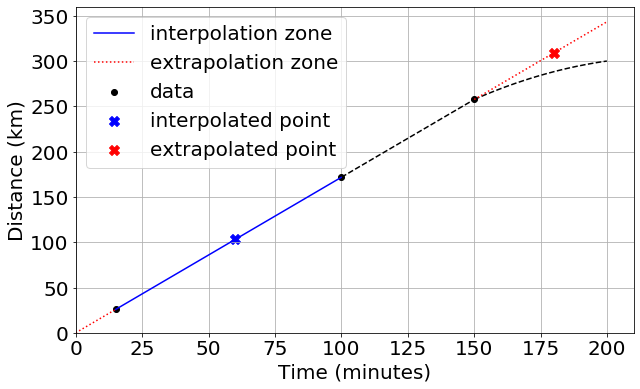
\includegraphics[width=0.7\textwidth]{figures/interp_example1.png}
  \caption{Samples of traveled distances at some time (black points). The blue and red crosses show an interpolated and an extrapolated point. It is clear how the extrapolation failed since after 150 minutes the relation between time and space changed.}
  \label{fig:samples_for_interpolation}
\end{figure}

Given two samples of the distance $s_1$ and $s_2$ taken at two different times $t_1$ and $t_2$ you can linearly interpolate to find the distance at an intermediate time using the following relation:

\begin{equation}
s = (1 - w)\cdot s_1 + w \cdot s_2
\end{equation}
where $t$ is the generic time at which we want to know the distance $s$ and $w = \cfrac{t - t_1}{t_2 - t_1}$.

\begin{attention}
\subsubsection{Derivation}
The equation of a line for two points $(t_1, s_1)$ and $(t_2, s_2)$ can be written as:

\begin{equation}
\frac{t - t_1}{t_2 - t_1} = \frac{s - s_1}{s_2 - s_1}
\end{equation}

Setting $w = \cfrac{t - t_1}{t_2 - t_1}$ and solving for $s$ we find the desired solution:

\begin{equation}
(s_2 - s_1)\cdot w = s - s_1\quad\implies\quad s = (1 - w)\cdot s_1 + w \cdot s_2
\end{equation}

This formula can also be understood as a weighted average where the weights are inversely related to the distance from the end points to the unknown point ($w_1 = (1 - w) = \cfrac{t_2 - t}{t_2 -t_1}, w_2 = w$), which means that the closer point has more "influence" than the farther point on the result.
\end{attention}

Back to our example, if
$s_1 = 25.75~\mathrm{km}\;(@t_1 = 15~\mathrm{min})$ and $s_2 = 171.7~\mathrm{km}\;(@t_2 = 100~\mathrm{min})$ let's find the distance traveled in 1 hour:

\begin{ipython}
s_1 = 25.75 # distance in km
t_1 = 15 	# elapsed time in minutes
s_2 = 171.7
t_2 = 100

t = 60
w = (t - t_1)/(t_2 - t_1)
s = (1 - w)*s_1 + w*s_2
print (f"{s:.1f} km")
\end{ipython}
\begin{ioutput}
103.0 km
\end{ioutput}

Instead of reinventing the wheel, \texttt{python} provides a function for interpolation, \texttt{numpy.interp}. 
To repeat our previous example:

\begin{ipython}
import scipy.interpolate import interp1d

t = [15, 100, 150]
s = [25.75, 171.7, 257.7]

inter = interp1d(t, s)	
print (f"{inter(60):1.f} km")
\end{ipython}
\begin{ioutput}
103.0 km
\end{ioutput}

\emph{Always interpret critically your results to guess if they make sense or not and avoid mistakes}. In the previous example we certainly expected something between 25.75 and 171.7~km (our range ends) furthermore since we are looking for the distance at a time which is almost halfway the considered interval, the result will be somehow in the middle, so around 100~km. This is indeed more or less what we have got. This simple kind of reasoning should be applied every time you have a result to quickly judge it.

\begin{curiosity}
\subsubsection{Epic Failure}
The Mars Climate Orbiter \emph{was} a 638~kg (1,407~lb), 326.7~M\$ space probe launched by NASA on December 11, 1998 to study Martian climate, atmosphere, and surface changes. 

On September 15, 1999, the necessary corrections to speed and direction of the probe were computed in order to place the spacecraft at an optimal position for an orbital insertion maneuver that would bring it around Mars at the proper altitude. 
But one week later communication with the spacecraft was permanently lost as it went into Martian orbital insertion. 

A committee of experts was created to investigate the reasons of 
such failure and they found out that the spacecraft encountered Mars at a lower than foreseen altitude causing either its destruction by atmospheric friction or making it bouncing against the atmosphere re-entering heliocentric orbit after leaving Mars.

The primary cause of this discrepancy was found in one piece of software (supplied by Lockheed Martin) that produced results in "Imperial" units,  while a second system (supplied by NASA) expected those results to be in SI units. Specifically, the software calculated the total impulse produced by thrust in \emph{pound-force seconds}. The trajectory calculation software then used these results, expected to be in \emph{newton seconds}, thus incorrect by a factor of 4.45, to update the predicted position of the spacecraft.
	
NASA took the entire responsibility for having vaporized about 300~M\$ in the Martian atmosphere, mainly for failing to make the appropriate checks and tests that would have caught this unit discrepancy~\cite{bib:mars}.	
\end{curiosity}

\subsubsection{Extrapolation}

If we believe the relation between our variables stays the same ($f(t)$ still linear), we can use the same formula to \emph{extrapolate} values \emph{outside} the range of the sample. For example if we keep the same constant velocity in our trip we could check the distance traveled after 3 hours:

\begin{ipython}
t = 180
w = (t - t_1)/(t_2 - t_1)
s = (1 - w)*s_1 + w*s_2

print (f"{s:.1f} km")
\end{ipython}
\begin{ioutput}
309.1 km
\end{ioutput}

In the given example the extrapolation failed since after minute 150 the traveled space ceased to be a linear function of time.

Notice that \texttt{interp1d} has \textbf{not} been designed for extrapolation, so if you ask for a value outside the range of sampled data it returns an error message.

%\begin{ipython}
%import numpy as np
%	
%t = [15, 100, 150]
%s = [25.75, 171.7, 257.7]
%	
%np.interp(180, t, s)
%\end{ipython}
%\begin{ioutput}
%257.7
%\end{ioutput}
%
%Pay attention to this aspect, for example by adding checks on the interpolation parameters, since the program works fine but could lead to weird results.

\subsection{Log-linear Interpolation}
\label{log-linear-interpolation}
When the function $f$ that we want to interpolate is an exponential we can fall back to the previous case by a simple variable transformation. 
Assume the following relationship between $p$ and $h$:

\begin{equation}
p = \mathrm{exp}(c \cdot h)
\end{equation}
Applying the logarithm to both sides of the equation gives:

\begin{equation}
s = \mathrm{log}(p) = \mathrm{log}(\mathrm{exp}(c \cdot h)) = c \cdot h
\end{equation}
so there is linear relation between the new variable $s$ and $h$. At this point we can use the results of the previous Section to interpolate for values of $s$, just remember to exponentiate the final result to get the correct $p$. In formulas:

\begin{align}
\label{eq:log_interp}
\begin{gathered}
w = \frac{h - h_1}{h_2 - h_1} \\
s = (1 - w)\cdot s_1 + w \cdot s_2\qquad (\textrm{now } s = \textrm{log}(p))\\
p = \textrm{exp}(s)
\end{gathered}
\end{align}

Let's see an example. Atmospheric pressure decreases with the altitude (i.e. the highest you flight the lower is the pressure) following an exponential law:

\begin{equation}
p = p_0\cdot e^{-\alpha h}
\end{equation}
where
\begin{itemize}
\tightlist
\item $h$ is the altitude
\item $p_0$ is the pressure at sea level
\item $\alpha$ is a constant
\end{itemize}

Taking the logarithm of each side of the equation we get a linear relation which can be interpolated as seen before:

\begin{equation}
s = \mathrm{log}(p) = \mathrm{log}(p_0\cdot e^{-\alpha h})\propto - \alpha \cdot h
\end{equation}

Now assume that we have measured
$p_1 = 90~\mathrm{kPa}\;(h_1 = 1000~\mathrm{m})$ and $p_2 = 40~\mathrm{kPa}\;(h_1 = 7000~\mathrm{m})$ what will be the atmospheric pressure on top of Mont Blanc ($4812~\mathrm{m}$) ? and on top of Mount Everest ($8848~\mathrm{m}$) ?

\begin{ipython}
# pressure on top of the Mont Blanc (interpolation)
from numpy import log, exp
from scipy.interpolate import interp1d

# first we take the logarithm of our measurements to use the linear
# relation to interpolate
h = [1000, 7000] # height in meters
s = [log(p) for p in [90, 40]] # logarithm of the pressure

inter = interp1d(h, s)
s = inter(4812)
print (f"{exp(s):.1f} kPa")
\end{ipython}
\begin{ioutput}
53.8 kPa
\end{ioutput}

If you want to extrapolate you need to use the homemade version of the interpolation algorithm
\begin{ipython}
h = 8848
h_1 = 1000
h_2 = 7000
s_1 = log(90)
s_2 = log(40)
w = (h - h_1)/(h_2 - h_1)
s = (1 - w)*s_1 + w*s_2

print (f"{exp(s):.1f} kPa")
\end{ipython}
\begin{ioutput}
31.2 kPa
\end{ioutput}

In this case we check our results by plotting the found pressures on top of the Wikipedia plot, see Fig~\ref{fig:Pvsh}.

\begin{figure}
\centering
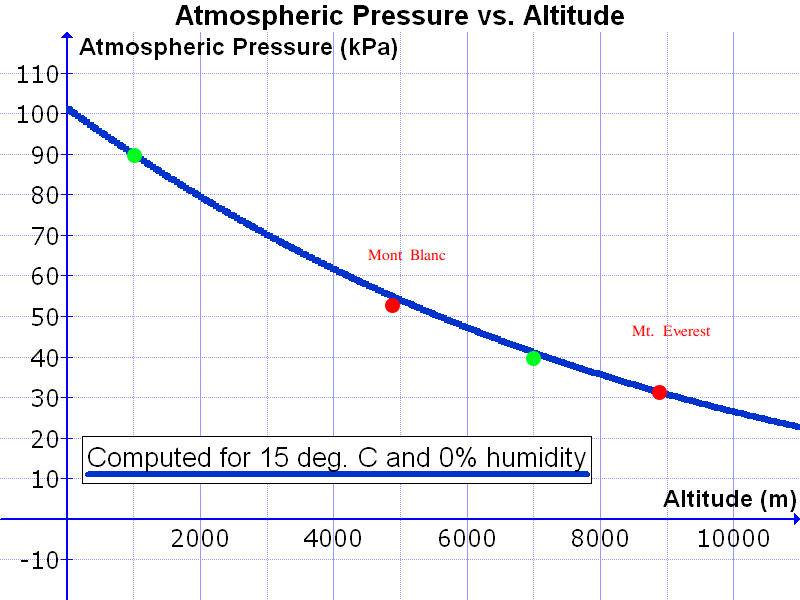
\includegraphics[width=0.7\linewidth]{figures/Atmospheric_Pressure_vs._Altitude.png}
\caption{Atmospheric pressure versus altitude (Wikipedia). Green points represent our measurements, red points represent interpolation/extrapolation.}
\label{fig:Pvsh}
\end{figure}

\subsection{Limitations of Interpolation}
Interpolation is just an approximation and works well when either the function $f$ is linear or we are trying to interpolate between two points that are close enough to believe that $f$ is almost linear in that interval.

It can be easily demonstrated that the linear approximation between two points of a given function $f(x)$ gets worse with the second derivative of the function that is approximated ($f''(x)$). This is intuitively correct: the "curvier" the function is, the worse the approximation made with simple linear interpolation becomes, see Fig.~\ref{fig:sine_interp} where we try to interpolate a sine function.

\begin{figure}
  \centering
  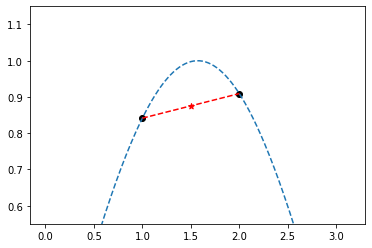
\includegraphics[width=0.7\textwidth]{figures/wrong_interp.png}
  \caption{Trying to approximate a sine function with a line is clearly not going to work unless the interpolation interval is very small.}
  \label{fig:sine_interp}
\end{figure}

To improve the approximation accuracy with complicated curves, an higher order polynomial can be used ($p(x)=a_0 + a_1\cdot x + a_2\cdot x^2+\cdots$), for example in the evaluation of natural logarithm or trigonometric functions. It has to be clear however that going to higher degrees does not always help~\cite{bib:runge}.

\section{Discount Curve Interpolation}
\label{discount-curve-interpolation}
With $D(T)$ (or $D(0,T)$) it is represented the discount factor corresponding to a spot rate $r$, and a time to cash flow $T$ (in years).

Discount factors are usually presented as curves (\emph{discount curves}) where each point represents a discount factor relative to a future date. Figure~\ref{fig:example_discount_curve} shows an example of discount curve.

\begin{figure}[htbp]
    \centering
	\includegraphics[width=0.7\linewidth]{figures/discount_curve}
	\caption{Example of discount curve.}
	\label{fig:example_discount_curve}
\end{figure}

Since discount curves are made of a discrete set of discount factors derived at some dates, we may need to find the factor at some different times; this is a typical financial application of interpolation.

\begin{finmarkets}
Since discount factors are an essential part for every financial calculation and we will keep using them everywhere, a \texttt{python} class which manages discount factors and curves is develop, using an object oriented approach.

This class, that we name \texttt{DiscountCurve}, should have as attributes
\begin{itemize}
	\tightlist
    \item an observation date which corresponds to $t=0$;
	\item a list of pillars dates specifying the value dates of the given discount factors, $t_0,...,t_{n-1}$;
	\item a list of given discount factors, $D(t_0),...,D(t_{n-1})$.
\end{itemize}

and at least a method to interpolate discount factors at a generic date. The input argument to this function will be the value date at which we want to interpolate. Since the discount factor can be expressed as an exponential the log-linear interpolation can be used:

\begin{equation}
	\begin{gathered}
		d(t_i)=\mathrm{ln}(D(t_i))\\
		d(t) = (1-w)d(t_i) + wd(t_{i+1});\quad w=\frac{t-t_i}{t_{i+1}-t_i}\\
		D(t) = \mathrm{exp}(d(t))
	\end{gathered}
\end{equation}
where $i$ is such that $t_i \le t \le t_{i+1}$

When dealing with discount factors we need to be careful though. \texttt{numpy.interp} only accepts list of numbers as argument (i.e. it doesn't know how to interpolate them). So we need to convert them before passing the dates to the interpolation function. This transformation will be implemented directly in the class constructor by replacing each date with the number of days from the observation date ($t_0$).
Furthermore we also attempted a simple code optimization: compute the input discount factors logarithm directly in the constructor in order to save some computation time with respect to doing the log at every call of the interpolation method. 
\end{finmarkets}

\begin{ipython}
from numpy import log, exp
from scipy.interpolate import interp1d
from datetime import date

class DiscountCurve:
    def __init__(self, obs_date, pillars, discount_factors):
#        self.obs_date = obs_date
        if obs_date not in pillars:
            pillars = [obs_date] + pillars
            discount_factors = np.insert(np.array(discount_factors), 0, 1)
        pillars = [p.toordinal() for p in pillars]
        log_df = [log(df) for df in self.discount_factors]
        self.inter = interp1d(pillars, log_df)
        
    def df(self, d):
        d = d.toordinal()
        if d < self.inter.x[0] or d > self.inter.x[-1]:
            print (f"Cannot extrapolate discount factors (date: {d}).")
            return None
        interpolated_log_discount_factor = np.interp(d_days, self.pillar_days, self.log_discount_factors)
        return exp(self.interp(d))
\end{ipython}

Using the discount curve data in \href{https://github.com/matteosan1/finance_course/raw/master/input_files/discount_factors_2022-10-05.xlsx}{\texttt{discount\_factors.xlsx}} instantiate the corresponding object and compute a discount factor.

\begin{finmarkets}
The \texttt{finmarkets} module is currently in the test repository of PyPi, the official collection of \texttt{python} modules. 
To install it in your working area just type 

\begin{ioutput}
pip install --index-url https://test.pypi.org/simple finmarkets
\end{ioutput}

(if you want to install it on Colab just prepend an exclamation mark to the previous command). The tool \texttt{pip} will take care of picking up the latest version of the package and of all the dependencies. You can explore the module with \texttt{help} command and in your program just import what you need with

\begin{ipython}
from finmarkets import DiscountCurve
\end{ipython}
\end{finmarkets}

\begin{ipython}
import pandas as pd
from datetime import date
from finmarkets import DiscountCurve
from dateutil.relativedelta import relativedelta

df = pd.read_excel("discount_factors.xlsx")

obs_date = date.today()
pillars = [today + relativedelta(months=i) for i in df['months']]
dfs = df['dfs'].values
dc = DiscountCurve(obs_date, pillars, dfs)
df_date = obs_date + relativedelta(days=195) #6.5 months
df0 = dc.df(df_date)
print (f"discount factor at {df_date}: {df0:.4f}")
\end{ipython}
\begin{ioutput}
discount factor at 2023-04-21: 0.9902
\end{ioutput}

A very useful way to check the correctness of a result is by plotting it. So let's see what the discount factor and the discount curve look like, Fig.~\ref{fig:linear_discount_curve}.

\begin{ipython}
from matplotlib import pyplot as plt

plt.plot(pillars[:10], dfs[:10], marker='o', markersize=10, 
         label="dfs")
plt.scatter(df_date, df0, marker='X', s=100, color='red', 
            label='interp. df')
plt.xticks(rotation=45)
plt.grid(True)
plt.legend()
plt.show()
\end{ipython}

%\begin{figure}[htb]
%	\centering
%	\includegraphics[width=0.7\textwidth]{figures/log_discount_curve}
%	\caption{Plot of the discount curve defined in the text and of the two computed discount factors with semi-log scale.}
%	\label{fig:log_discount_curve}
%\end{figure}
%\noindent
%Let's see what it looks like when plotted on a linear graph too, Fig.~\ref{fig:linear_discount_curve}.
%\begin{ipython}
%plt.plot(pillar_dates, discount_factors, marker='o')
%plt.plot(d0, df0, marker='X')
%plt.plot(d1, df1, marker='X')
%plt.gca().xaxis.set_major_formatter(mdates.DateFormatter('%m/%d/%Y'))
%plt.gca().xaxis.set_major_locator(mdates.YearLocator())
%plt.grid(True)
%plt.show()
%\end{ipython}

\begin{figure}[htb]
	\centering
	\includegraphics[width=0.7\textwidth]{figures/linear_discount_curve}
	\caption{Plot of the discount curve defined in the text and of the discount factor with linear scale.}
	\label{fig:linear_discount_curve}
\end{figure}

\section{Forward Rates}
\label{calculating-forward-rates}
A forward rate is an interest rate applicable to a financial transaction that will take place in the future. It can be considered as the market's expectation for future prices and can serve as an indicator of how it believes will perform.

Contrary the \emph{spot rate} is used by buyers and sellers looking to make an immediate purchase or sale, and it cannot be an indicator of market expectations.

Forward rates are calculated from the spot rate by exploiting the no arbitrage condition which states that investing at rate $r_1$ for the period $(0, T_1)$ and then \emph{re-investing} at rate $r_{1,2}$ for the time period $(T_1, T_2)$ is equivalent to invest at rate $r_2$ for the full time period $(0, T_2)$. Essentially two investors shouldn't be able to earn money from arbitraging between different interest periods. That said:

\begin{equation}
(1+r_1 T_1)[1+r_{1,2}(T_2 - T_1)] = 1 + r_2 T_2
\label{eq:no_arbitrage_r}
\end{equation}
Solving for $r_{1,2}$ leads to

\begin{equation}
F(T_1, T_2) = r_{1,2} = \frac{1}{T_2 - T_1}\Big(\frac{1+r_2 T_2}{1+r_1 T_1} - 1 \Big)
\label{eq:forward_rate_simple}
\end{equation}
\vspace{1cm}
The same expression in terms of the discount factor of Eq.~\ref{eq:discount_factor} becomes
\begin{equation}
F(T_1, T_2) = \frac{1}{T_2 - T_1}\Big(\frac{D(0, T_1)}{D(0, T_2)} - 1 \Big)
\end{equation}
Considering continuously compounded rates instead Eq.~\ref{eq:no_arbitrage_r} can be written as
\begin{equation}
\begin{gathered}
e^{r_{2}T_{2}}=e^{r_{1}T_{1}}\cdot \ e^{r_{1,2} (T_{2}-T_{1})} \\
\textrm{log}\left(e^{r_{2}T_{2}}\right)=\textrm{log}\left(e^{r_{1}T_{1}+ r_{1,2} (T_{2}-T_{1})}\right) \\
r_{2}T_{2}=r_{1}T_{1}+r_{1,2}(T_{2}-T_{1})\implies r_{1,2} = \cfrac{r_2 T_2 - r_1 T_1}{T_2 - T_1} 
\end{gathered}
\end{equation}
and the corresponding expression for the forward rate is
\begin{equation}
F(T_1, T_2) = r_{1,2} = \frac {1}{T_{2}-T_{1}}(\ln D(0,T_{1})-\ln D(0,T_{2}))
\quad(\textrm{since now } D(0, T_i)=e^{-r_i T_i})
\label{eq:forward_rate_continous}
\end{equation}

\begin{finmarkets}
The \texttt{ForwardRateCurve} class of the \texttt{finmarkets} module computes forward rates at any arbitrary date, given a set of spot rates. This class is quite similar to \texttt{DiscountCurve}, it has two methods: one to interpolate spot rates, another to actually compute the forward rates.

In order to successfully interpolate the rates, dates need to be converted to numbers by evaluating the number of days since a reference date (the observation date in this implementation). Also the interpolation date is checked to avoid extrapolations, if it is outside the known range a warning will be printed out and the calculation stopped.
\end{finmarkets}

\begin{ipython}
from scipy.interpolate import interp1d

class ForwardRateCurve:
    def __init__(self, obs_date, pillars, rates):
        self.obs_date = obs_date
        pillars = [(p - obs_date).days/365 for p in pillars]
        self.inter = interp1d(pillars, rates)

    def interp_rate(self, d):
        d_frac = (d - self.obs_date).days/365
        if d < self.obs_date or d_frac > self.inter.x[-1]:
            print (f"Cannot extrapolate rates (date: {d}).")
            return None, None
        else:
            return d_frac, self.inter(d_frac)

    def forward_rate(self, d1, d2):
        d1_frac, r1 = self.interp_rate(d1)
        d2_frac, r2 = self.interp_rate(d2)
        if d1_frac is None or d2_frac is None:
            return None
        else:
            return (r2*d2_frac - r1*d1_frac)/(d2_frac - d1_frac)
\end{ipython}

As an example let's compute a forward rate.
\begin{ipython}
from finmarkets import ForwardRateCurve
from datetime import date
from dateutil.relativedelta import relativedelta

obs_date = data.today()

pillar_dates = [obs_date,
                obs_date + relativedelta(months=12),
                obs_date + relativedelta(months=30)]
rates = [0.0221, 0.0241, 0.025]

fc = ForwardRateCurve(obs_date, pillar_dates, rates)
t1 = obs_date + relativedelta(months=12)
t2 = obs_date + relativedelta(months=24)
print (f"F({t1}, {t2}) = {fc.forward_rate(t1, t2):.4f}")
\end{ipython}
\begin{ioutput}
F(2021-01-01, 2022-01-01) = 0.0253
\end{ioutput}

\section{Multi-curve Framework}
\label{sec:financial-crisis}

% aggiungere un pezzettino dell'articolo di Mercurio

Prior to the 2008 financial crisis, inter-bank deposits posed little credit/liquidity issues, inter-bank lending rates (e.g. LIBOR, EURIBOR) were essentially a good proxy for risk free rates. Basis swap spreads were negligible and thereby neglected. 

Looking at the historical series of the EURIBOR (6M) rate versus the EONIA Overnight Indexed Swap (OIS-6M) rate over the time interval 2006-2011 in Fig.~\ref{fig:credit_crunch} it becomes apparent how before August 2007 the two rates display strictly overlapping trends differing of no more than 6 bps.

\begin{figure}[htb]
	\centering
	\includegraphics[width=0.9\linewidth]{figures/credit_crunch.png}
	\caption{Historical series of EURIBOR 6M rate versus EONIA OIS 6M rate. The corresponding spread 
		is shown on the right axis (Jan. 06 - Dec. 10 window, source: Bloomberg).}
	\label{fig:credit_crunch}
\end{figure}

A single yield curve constructed out of selected deposit, FRA and swap rates, served both the cash flow projection and discounting purposes.

During the 2008 financial crisis, the failure of some banks however proved that inter-bank lending rates were not risk-free. Meanwhile there was also significant counter-party credit risk arising from derivative transactions that were not subjected to collateral. Basis swap spreads greatly widened, and persist to this day. 

Still looking at Fig.~\ref{fig:credit_crunch} it is clear how in August 2007 a sudden increase of the EURIBOR rate and a simultaneous decrease of the OIS rate led to the explosion of the corresponding basis spread, touching the peak of 222 bps in October 2008, when Lehman Brothers filed for bankruptcy. Successively the basis has sensibly reduced and stabilized between 40 and 60 bps (notice that the pre-crisis level has never been recovered). The same effect is observed for other similar couples of series, e.g. EURIBOR 3M vs OIS 3M.

The existence of such significant basis swap spread reflects the fact that after the crisis interest rate market has been segmented into subareas corresponding to instruments with different underlying rate tenors, characterized by different rate dynamics. 

Traditional single curve based pricing approach ignores these differences. It mixes different underlying rate tenors and incorporates different rate dynamics, eventually leading to inconsistency.
%After the crisis, the market practice has thus evolved to take into account the new market information (e.g. the basis swap spreads, collateralization, etc.), that translate into the additional requirement of homogeneity and funding. The homogeneity requirement means that interest rate derivatives with a given underlying rate tenor must be priced and hedged using vanilla interest rate market instruments with the same underlying. The funding requirement means that the discount rate of any cash flow generated by the derivative must be consistent, by no-arbitrage, with the funding rate associated with that cash flow. 

Driven by the crisis, many derivative contracts have been updated to include permissible credit mitigants for a transaction, such as netting and collateralization in cash. Since standard agreements stipulate daily margination on collateral and the cash collateral earns a return at overnight rate, overnight rate becomes a natural choice for the risk-free discount rate or the funding rate. This is referred to as \emph{OIS discounting}.

Due to the large spread between risk free rate and inter-bank lending rate during and after 2008 financial crisis it is not possible anymore to use a single curve for discounting and derivative valuation. The traditional single curve used for both cash flow projection and discounting turned out to be obsolete. The markets have since nearly switched to \emph{multi-curve framework}. 

For example, if we want to calculate the net present value (NPV) of a forward 6-month EURIBOR coupon, we need to simultaneously use two different discount curves: 

\begin{itemize}
\tightlist
\item the 6-month EURIBOR curve for determining the forward rate;
\item the \euro STR curve for discounting the expected cash flow.
\end{itemize}

%The reason of the abrupt divergence between the Euribor and OIS rates can be explained by considering both the monetary policy decisions adopted by international authorities in response to the financial turmoil, and the impact of the credit crunch on both credit and liquidity risk perception of the market, coupled with the different financial meaning and dynamics of these rates.

%\begin{itemize}
%\tightlist
%\item
%  The Euribor rate is the reference rate for over-the-counter (OTC)
%  transactions in the Euro area. It is defined as the rate at which
%  Euro inter-bank deposits are being offered within the EMU zone by one
%  prime bank to another at 11:00 a.m. Brussels time. The rate fixings
%  for a strip of 15 maturities (from one day to one year) are
%  constructed as the average of the rates submitted (excluding the
%  highest and lowest 15\% tails) by a panel of 42 banks, selected
%  among the EU banks with the highest volume of business in the Euro
%  zone money markets, plus some large international bank from non-EU
%  countries with important euro zone operations. \emph{Thus, Euribor
%  rates reflect the average cost of funding of banks in the inter bank
%  market at each given maturity. During the crisis the solvency and
%  solidity of the whole financial sector was brought into question and
%  the credit and liquidity risk and uremia associated to inter-bank
%  counter-parties sharply increased.} The Euribor rates immediately
%  reflected these dynamics and raise to their highest values over more
%  than 10 years. As seen in the plot above, the Euribor 6M rate suddenly
%  increased on August 2007 and reached 5.49\% on 10th October 2008.
%\item
%  The EONIA rate is the reference rate for overnight OTC transactions in
%  the Euro area. It is constructed as the average rate of the overnight
%  transactions (one day maturity deposits) executed during a given
%  business day by a panel of banks on the inter-bank money market,
%  weighted with the corresponding transaction volumes. \emph{The EONIA
%  Contribution Panel coincides with the Euribor Contribution Panel, thus
%  EONIA rate includes information on the short term (overnight)
%  liquidity expectations of banks in the Euro money market. It is also
%  used by the European Central Bank (ECB) as a method of effecting and
%  observing the transmission of its monetary policy actions. During the
%  crisis the central banks were mainly concerned about stabilizing the
%  level of liquidity in the market, thus they reduced the level of the
%  official rates.} Furthermore, the daily tenor of the EONIA rate makes
%  negligible the credit and liquidity risks reflected on it: for this
%  reason the OIS rates are considered the best proxies available in the
%  market for the risk-free rate.
%\end{itemize}

%Our financial library has to implement the following calculation
%
%\[\mathrm{NPV} = D_{\mathrm{EONIA}}(T_1) \cdot \frac{1}{T_2-T_1}\Big(\frac{D_{\mathrm{LIBOR}}(T_1)}{D_{\mathrm{LIBOR}}(T_2)} - 1 \Big)\]
%\noindent
%In order to do so we can extend the \texttt{DiscountCurve} class with a \texttt{forward\_rate} method
%
%\begin{ipython}
%class DiscountCurve:
%    ...
%    def forward_rate(self, d1, d2):
%        return (self.df(d1) / self.df(d2) - 1.0) * \
%            (365.0 / ((d2 - d1).days))
%\end{ipython}

As an example let's define \euro STR and EURIBOR curves and compute the net present value of the forward 6-month EURIBOR coupon mentioned before.

\begin{ipython}
from finmarkets import DiscountCurve, ForwardRateCurve
from numpy import exp
from dateutil.relativedelta import relativedelta
from datetime import date

obs_date = date.today()
t1 = obs_date + relativedelta(months=3)
t2 = obs_date + relativedelta(months=9)
pillar_dates_estr = [obs_date, 
                     obs_date + relativedelta(months=12),
                     obs_date + relativedelta(months=34)]
estr_rates = [1.0, 0.97, 0.72]
pillar_dates_euribor = [obs_date, 
                        obs_date + relativedelta(months=5), 
                        obs_date + relativedelta(months=12)]
euribor = [0.005, 0.01, 0.015]

estr_curve = DiscountCurve(obs_date, pillar_dates_estr, estr_rates) 
euribor_curve = ForwardRateCurve(obs_date, pillar_dates_euribor, euribor) 

C = estr_curve.df(t1) * euribor_curve.forward_rate(t1, t2)
t1_frac, r1 = euribor_curve.interp_rate(t1)
C_pre2008 = exp(-r1*t1_frac) * euribor_curve.forward_rate(t1, t2)

print (f"C post 2008: {C:.5f} EUR")
print (f"C pre 2008: {C_pre2008:.5f} EUR")
\end{ipython}
\begin{ioutput}
C post 2008: 0.01513 EUR
C pre 2008: 0.01522 EUR
\end{ioutput}

%\subsection{Transitioning away from LIBOR~\cite{bib:str}}
%A working group on euro risk-free rates was established to identify and recommend risk free rates that could serve as a basis for an alternative to current benchmarks used in a variety of financial instruments and contracts in the euro area, such as the euro overnight index average (EONIA) and the euro inter-bank offered rate (EURIBOR). 
%
%The group recommended on September 2018 that the euro short-term rate (\euro STR) be used as the risk-free rate for the euro area and is now focused on supporting the market with transitioning.
%The ECB published the \euro STR for the first time on 2nd October 2019, reflecting trading activity on 1st October 2019.
%
%The working group recommends that market participants should gradually replace EONIA with the \euro STR as a reference rate for all products and contracts and make all necessary adjustments for using the \euro STR as their standard benchmark The working group recommends the \euro STR plus a fixed spread of 8.5
%basis points as the EONIA fallback rate for all products and purposes. The working group recommends that market participants should: consider, whenever feasible and appropriate, no longer entering into new contracts referencing EONIA, in particular new contracts maturing after 31 December 2021, as EONIA will cease to exist after that date.
%
%%The working group is also looking at identifying fallbacks for
%%EURIBOR based on the STR. Both backward and forward-looking
%%options are being considered. As part of its work on forward-looking
%%options, in March 2019 the working group recommended a
%%methodology based on (tradable) overnight index swap (OIS) quotes
%%for calculating a STR-based forward-looking term structure and later
%%invited benchmark administrators to express their interest in
%%producing such a term structure.

\section*{Exercises}
\begin{question}
Python has a useful command called \texttt{assert} which can be used for checking that a given condition is satisfied, and raising an error if the condition is not satisfied.

The following line does not cause an error, in fact it does nothing since 1 is lower than 2, hence the condition is met.

\lstinline[language=iPython]|assert 1 < 2|

\noindent
This causes an error (the condition is evaluated to false). 

\lstinline[language=iPython]|assert 1 > 2|

\noindent
\texttt{assert} can take a second argument with a message to display in case of failure.

\lstinline[language=iPython]|assert 1 > 2, "Two is greater than one"|

\noindent
Now takes the \texttt{df} function from the Chapter on Discounting and modify it by adding some assertions to check that:

\begin{itemize}
\item the pillar date list contains at least 2 elements;
\item the pillar date list has the same length as the discount factor one;
\item the first pillar date is equal to the today's date;
\item the value date (first argument \texttt{d}) is greater or equal to the first pillar date and also less than or equal to the last pillar date.
\end{itemize}

Then try using the function with some invalid data to make sure that your assertions are correctly checking the desired conditions
\end{question}

\begin{solution}
\end{solution}

\begin{ipython}
# import modules and objects that we need
from datetime import date
import numpy
import math

today_date = date(2017, 10, 1)
pillar_dates = [date(2017, 10, 1),
date(2018, 10, 1),
date(2019, 10, 1)]
discount_factors = [1.0, 0.95, 0.8]

def df(d, observation_date, pillar_dates, discount_factors):
    ############## CHECKS ################
    assert len(pillar_dates) >= 2, " need at least 2 pillar dates"
    assert len(pillar_dates) == len(discount_factors), \
        "number of pillar dates should be equal to \
         the number of pillar discount factors"
    assert observation_date == pillar_dates[0], \
        "first pillar date should be the observation date"
    assert pillar_dates[0] <= d <= pillar_dates[-1], \
        "Invalid value date %s" % (d)
    ############## END OF CHECKS ################
    log_discount_factors = []
    for discount_factor in discount_factors:
        log_discount_factors.append(math.log(discount_factor))
    pillar_days = []
    for pillar_date in pillar_dates:
        pillar_days.append((pillar_date - observation_date).days)
    d_days = (d - observation_date).days
    interpolated_log_discount_factor = \
        numpy.interp(d_days, pillar_days, log_discount_factors)
    return math.exp(interpolated_log_discount_factor)

df(date(2019, 1, 1), today_date, pillar_dates, discount_factors)

0.9097285910181567
\end{ipython}

%\begin{question}
%Copy into the file \texttt{finmarkets.py} the function used to compute Black Scholes formula used in Ex.~\ref{ex:BS2}. This is another utility for our financial library. Then repeat Ex.~\ref{ex:BS2} now using the version of the Black and Scholes formula in the \texttt{finmarkets} module.
%\end{question}
%
%\begin{solution}
%\begin{tcolorbox}[size=fbox, boxrule=1pt, colback=cellbackground, colframe=cellborder]
%\begin{Verbatim}[commandchars=\\\{\}]
%\PY{k}{import} \PY{n}{finmarkets}
%        
%\PY{n}{s} \PY{o}{=} \PY{l+m+mi}{800}
%\PY{c+c1}{\PYZsh{} strikes expressed as \PYZpc{} of spot price}
%\PY{n}{moneyness} \PY{o}{=} \PY{p}{[} \PY{l+m+mf}{0.5}\PY{p}{,} \PY{l+m+mf}{0.75}\PY{p}{,} \PY{l+m+mf}{0.825}\PY{p}{,} \PYZbs{}
%             \PY{l+m+mf}{1.0}\PY{p}{,} \PY{l+m+mf}{1.125}\PY{p}{,} \PY{l+m+mf}{1.25}\PY{p}{,} \PY{l+m+mf}{1.5} \PY{p}{]}
%\PY{n}{vol} \PY{o}{=} \PY{l+m+mf}{0.3}
%\PY{n}{ttm} \PY{o}{=} \PY{l+m+mf}{0.75}
%\PY{n}{r} \PY{o}{=} \PY{l+m+mf}{0.005}
%
%\PY{n}{result} \PY{o}{=} \PY{p}{\PYZob{}}\PY{p}{\PYZcb{}}
%\PY{k}{for} \PY{n}{m} \PY{o+ow}{in} \PY{n}{moneyness}\PY{p}{:}
%    \PY{n}{result}\PY{p}{[}\PY{n}{s}\PY{o}{*}\PY{n}{m}\PY{p}{]} \PY{o}{=} \PY{n}{finmarkets.call}\PY{p}{(}\PY{n}{s}\PY{p}{,} \PY{n}{m}\PY{o}{*}\PY{n}{s}\PY{p}{,} \PY{n}{r}\PY{p}{,} \PY{n}{vol}\PY{p}{,} \PY{n}{ttm}\PY{p}{)}
%\PY{n}{result}
%
%\{400.0: 401.66074527896365,
%  600.0: 213.9883852521275,
%  660.0: 166.85957363897393,
%  800.0: 84.03697017660357,
%  900.0: 47.61880394696229,
%  1000.0: 25.632722952585738,
%  1200.0: 6.655275227771156\}
%\end{Verbatim}
%\end{tcolorbox}
%\end{solution}

%\begin{question}
%Following the steps outlined in Chapter Discount Factors, implement a \texttt{DiscountCurve} class and add it to \texttt{finmarkets} module. The class should have as attributes the pillar dates and the corresponding discount factors and two methods, one to interpolate discount factors and another to calculate forward rates.
%Finally using that class compute the forward 6M LIBOR coupon using the curves given below in pre and post 2008 crisis way.
%
%\textbf{Input:}
%\begin{Shaded}
%\begin{Highlighting}[]
%\NormalTok{observation_date }\OperatorTok{=}\NormalTok{ date (}\DecValTok{2020}\NormalTok{, }\DecValTok{1}\NormalTok{, }\DecValTok{1}\NormalTok{)}
%\NormalTok{t1 }\OperatorTok{=}\NormalTok{ date(}\DecValTok{2020}\NormalTok{,}\DecValTok{4}\NormalTok{, }\DecValTok{1}\NormalTok{)}
%\NormalTok{t2 }\OperatorTok{=}\NormalTok{ date(}\DecValTok{2020}\NormalTok{, }\DecValTok{10}\NormalTok{, }\DecValTok{1}\NormalTok{)}
%
%\CommentTok{# for EONIA}
%\NormalTok{pillar_dates_eonia }\OperatorTok{=}\NormalTok{ [date(}\DecValTok{2020}\NormalTok{ , }\DecValTok{1}\NormalTok{ ,}\DecValTok{1}\NormalTok{), }
%\NormalTok{                      date(}\DecValTok{2021}\NormalTok{, }\DecValTok{1}\NormalTok{, }\DecValTok{1}\NormalTok{), }
%\NormalTok{                      date(}\DecValTok{2022}\NormalTok{, }\DecValTok{10}\NormalTok{ ,}\DecValTok{1}\NormalTok{)]}
%\NormalTok{discount_factors_eonia }\OperatorTok{=}\NormalTok{ [}\FloatTok{1.0}\NormalTok{, }\FloatTok{0.97}\NormalTok{, }\FloatTok{0.72}\NormalTok{]}
%
%\CommentTok{# for LIBOR 6M}
%\NormalTok{pillar_dates_libor }\OperatorTok{=}\NormalTok{ [date(}\DecValTok{2020}\NormalTok{, }\DecValTok{1}\NormalTok{ ,}\DecValTok{1}\NormalTok{), }
%\NormalTok{                      date(}\DecValTok{2020}\NormalTok{, }\DecValTok{6}\NormalTok{, }\DecValTok{1}\NormalTok{), }
%\NormalTok{                      date(}\DecValTok{2020}\NormalTok{, }\DecValTok{12}\NormalTok{ ,}\DecValTok{1}\NormalTok{)]}
%\NormalTok{discount_factors_libor }\OperatorTok{=}\NormalTok{ [}\FloatTok{1.0}\NormalTok{, }\FloatTok{0.95}\NormalTok{, }\FloatTok{0.90}\NormalTok{]}
%\end{Highlighting}
%\end{Shaded}
%\end{question}
%
%\begin{solution}
%\begin{tcolorbox}[size=fbox, boxrule=1pt, pad at break*=1mm,colback=cellbackground, colframe=cellborder]
%\begin{Verbatim}[commandchars=\\\{\}]
%\PY{k+kn}{import} \PY{n+nn}{math}
%\PY{k+kn}{import} \PY{n+nn}{numpy}
%\PY{k+kn}{from} \PY{n+nn}{datetime} \PY{k}{import} \PY{n}{date}
%
%\PY{k}{class} \PY{n+nc}{DiscountCurve}\PY{p}{:}
%
%    \PY{k}{def} \PY{n+nf}{\PYZus{}\PYZus{}init\PYZus{}\PYZus{}}\PY{p}{(}\PY{n+nb+bp}{self}\PY{p}{,} \PY{n}{today}\PY{p}{,} \PY{n}{pillar\PYZus{}dates}\PY{p}{,} \PY{n}{discount\PYZus{}factors}\PY{p}{)}\PY{p}{:}
%        \PY{n+nb+bp}{self}\PY{o}{.}\PY{n}{today} \PY{o}{=} \PY{n}{today}
%        \PY{n+nb+bp}{self}\PY{o}{.}\PY{n}{pillar\PYZus{}dates} \PY{o}{=} \PY{n}{pillar\PYZus{}dates}
%        \PY{n+nb+bp}{self}\PY{o}{.}\PY{n}{discount\PYZus{}factors} \PY{o}{=} \PY{n}{discount\PYZus{}factors}
%
%    \PY{k}{def} \PY{n+nf}{df}\PY{p}{(}\PY{n+nb+bp}{self}\PY{p}{,} \PY{n}{d}\PY{p}{)}\PY{p}{:}
%        \PY{n}{log\PYZus{}discount\PYZus{}factors} \PY{o}{=} \PYZbs{}
%          \PY{p}{[}\PY{n}{math}\PY{o}{.}\PY{n}{log}\PY{p}{(}\PY{n}{discount\PYZus{}factor}\PY{p}{)} 
%           \PY{k}{for} \PY{n}{discount\PYZus{}factor} \PY{o+ow}{in} \PY{n+nb+bp}{self}\PY{o}{.}\PY{n}{discount\PYZus{}factors}\PY{p}{]}
%        \PY{n}{pillar\PYZus{}days} \PY{o}{=} \PY{p}{[}\PY{p}{(}\PY{n}{pillar\PYZus{}date} \PY{o}{\PYZhy{}} \PY{n+nb+bp}{self}\PY{o}{.}\PY{n}{today}\PY{p}{)}\PY{o}{.}\PY{n}{days} 
%                       \PY{k}{for} \PY{n}{pillar\PYZus{}date} \PY{o+ow}{in} \PY{n+nb+bp}{self}\PY{o}{.}\PY{n}{pillar\PYZus{}dates}\PY{p}{]}
%        \PY{n}{d\PYZus{}days} \PY{o}{=} \PY{p}{(}\PY{n}{d} \PY{o}{\PYZhy{}} \PY{n+nb+bp}{self}\PY{o}{.}\PY{n}{today}\PY{p}{)}\PY{o}{.}\PY{n}{days}
%        \PY{n}{interpolated\PYZus{}log\PYZus{}discount\PYZus{}factor} \PY{o}{=} \PYZbs{}
%            \PY{n}{numpy}\PY{o}{.}\PY{n}{interp}\PY{p}{(}\PY{n}{d\PYZus{}days}\PY{p}{,} \PY{n}{pillar\PYZus{}days}\PY{p}{,} \PY{n}{log\PYZus{}discount\PYZus{}factors}\PY{p}{)}
%        \PY{k}{return} \PY{n}{math}\PY{o}{.}\PY{n}{exp}\PY{p}{(}\PY{n}{interpolated\PYZus{}log\PYZus{}discount\PYZus{}factor}\PY{p}{)}
%
%    \PY{k}{def} \PY{n+nf}{forward\PYZus{}rate}\PY{p}{(}\PY{n+nb+bp}{self}\PY{p}{,} \PY{n}{d1}\PY{p}{,} \PY{n}{d2}\PY{p}{)}\PY{p}{:}
%        \PY{k}{return} \PY{p}{(}\PY{n+nb+bp}{self}\PY{o}{.}\PY{n}{df}\PY{p}{(}\PY{n}{d1}\PY{p}{)} \PY{o}{/} \PY{n+nb+bp}{self}\PY{o}{.}\PY{n}{df}\PY{p}{(}\PY{n}{d2}\PY{p}{)} \PY{o}{\PYZhy{}} \PY{l+m+mf}{1.0}\PY{p}{)} \PY{o}{*} \PYZbs{}
%                \PY{p}{(}\PY{l+m+mf}{365.0} \PY{o}{/} \PY{p}{(}\PY{p}{(}\PY{n}{d2} \PY{o}{\PYZhy{}} \PY{n}{d1}\PY{p}{)}\PY{o}{.}\PY{n}{days}\PY{p}{)}\PY{p}{)}
%\end{Verbatim}
%\end{tcolorbox}
%
%\begin{tcolorbox}[breakable, size=fbox, boxrule=1pt, pad at break*=1mm,colback=cellbackground, colframe=cellborder]
%\begin{Verbatim}[commandchars=\\\{\}]
%\PY{k+kn}{from} \PY{n+nn}{finmarkets} \PY{k}{import} \PY{n}{DiscountCurve}
%
%\PY{n}{observation\PYZus{}date} \PY{o}{=} \PY{n}{date} \PY{p}{(}\PY{l+m+mi}{2020}\PY{p}{,} \PY{l+m+mi}{1}\PY{p}{,} \PY{l+m+mi}{1}\PY{p}{)}
%\PY{n}{t1} \PY{o}{=} \PY{n}{date}\PY{p}{(}\PY{l+m+mi}{2020}\PY{p}{,}\PY{l+m+mi}{4}\PY{p}{,} \PY{l+m+mi}{1}\PY{p}{)}
%\PY{n}{t2} \PY{o}{=} \PY{n}{date}\PY{p}{(}\PY{l+m+mi}{2020}\PY{p}{,} \PY{l+m+mi}{10}\PY{p}{,} \PY{l+m+mi}{1}\PY{p}{)}
%
%\PY{c+c1}{\PYZsh{} for EONIA}
%\PY{n}{pillar\PYZus{}dates\PYZus{}eonia} \PY{o}{=} \PY{p}{[}\PY{n}{date}\PY{p}{(}\PY{l+m+mi}{2020} \PY{p}{,} \PY{l+m+mi}{1} \PY{p}{,}\PY{l+m+mi}{1}\PY{p}{)}\PY{p}{,} 
%                      \PY{n}{date}\PY{p}{(}\PY{l+m+mi}{2021}\PY{p}{,} \PY{l+m+mi}{1}\PY{p}{,} \PY{l+m+mi}{1}\PY{p}{)}\PY{p}{,} 
%                      \PY{n}{date}\PY{p}{(}\PY{l+m+mi}{2022}\PY{p}{,} \PY{l+m+mi}{10} \PY{p}{,}\PY{l+m+mi}{1}\PY{p}{)}\PY{p}{]}
%\PY{n}{discount\PYZus{}factors\PYZus{}eonia} \PY{o}{=} \PY{p}{[}\PY{l+m+mf}{1.0}\PY{p}{,} \PY{l+m+mf}{0.97}\PY{p}{,} \PY{l+m+mf}{0.72}\PY{p}{]}
%
%\PY{c+c1}{\PYZsh{} for LIBOR 6M}
%\PY{n}{pillar\PYZus{}dates\PYZus{}libor} \PY{o}{=} \PY{p}{[}\PY{n}{date}\PY{p}{(}\PY{l+m+mi}{2020}\PY{p}{,} \PY{l+m+mi}{1} \PY{p}{,}\PY{l+m+mi}{1}\PY{p}{)}\PY{p}{,} 
%                      \PY{n}{date}\PY{p}{(}\PY{l+m+mi}{2020}\PY{p}{,} \PY{l+m+mi}{6}\PY{p}{,} \PY{l+m+mi}{1}\PY{p}{)}\PY{p}{,} 
%                      \PY{n}{date}\PY{p}{(}\PY{l+m+mi}{2020}\PY{p}{,} \PY{l+m+mi}{12} \PY{p}{,}\PY{l+m+mi}{1}\PY{p}{)}\PY{p}{]}
%\PY{n}{discount\PYZus{}factors\PYZus{}libor} \PY{o}{=} \PY{p}{[}\PY{l+m+mf}{1.0}\PY{p}{,} \PY{l+m+mf}{0.95}\PY{p}{,} \PY{l+m+mf}{0.90}\PY{p}{]}
%
%
%\PY{n}{eonia\PYZus{}curve} \PY{o}{=} \PY{n}{DiscountCurve}\PY{p}{(}\PY{n}{observation\PYZus{}date}\PY{p}{,} 
%                            \PY{n}{pillar\PYZus{}dates\PYZus{}eonia}\PY{p}{,} 
%                            \PY{n}{discount\PYZus{}factors\PYZus{}eonia}\PY{p}{)}
%\PY{n}{libor\PYZus{}curve} \PY{o}{=} \PY{n}{DiscountCurve}\PY{p}{(}\PY{n}{observation\PYZus{}date}\PY{p}{,} 
%                            \PY{n}{pillar\PYZus{}dates\PYZus{}libor}\PY{p}{,} 
%                            \PY{n}{discount\PYZus{}factors\PYZus{}libor}\PY{p}{)}
%
%
%\PY{n}{npv} \PY{o}{=} \PY{n}{eonia\PYZus{}curve}\PY{o}{.}\PY{n}{df}\PY{p}{(}\PY{n}{t1}\PY{p}{)} \PY{o}{*} \PY{n}{libor\PYZus{}curve}\PY{o}{.}\PY{n}{forward\PYZus{}rate}\PY{p}{(}\PY{n}{t1}\PY{p}{,} \PY{n}{t2}\PY{p}{)}
%
%\PY{c+c1}{\PYZsh{} Compute it in the pre\PYZhy{}2008 way}
%\PY{n}{npv\PYZus{}pre2008} \PY{o}{=} \PY{n}{libor\PYZus{}curve}\PY{o}{.}\PY{n}{df}\PY{p}{(}\PY{n}{t1}\PY{p}{)} \PY{o}{*} \PY{n}{libor\PYZus{}curve}\PY{o}{.}\PY{n}{forward\PYZus{}rate}\PY{p}{(}\PY{n}{t1}\PY{p}{,} \PY{n}{t2}\PY{p}{)}
%
%\PY{n+nb}{print} \PY{p}{(}\PY{l+s+s2}{\PYZdq{}}\PY{l+s+s2}{NPV post 2008:}\PY{l+s+s2}{\PYZdq{}}\PY{p}{,} \PY{n}{npv}\PY{p}{)}
%\PY{n+nb}{print} \PY{p}{(}\PY{l+s+s2}{\PYZdq{}}\PY{l+s+s2}{NPV pre 2008:}\PY{l+s+s2}{\PYZdq{}}\PY{p}{,} \PY{n}{npv\PYZus{}pre2008}\PY{p}{)}
%
%NPV post 2008: 0.11533243116069992
%NPV pre 2008: 0.11269481011359303
%\end{Verbatim}
%\end{tcolorbox}
%\end{solution}
%
%\begin{question}
%Write a ForwardRateCurve class (for EURIBOR/LIBOR rate curve) which
%doesn't compute discount factors but only interplatates forward rates;
%then add it to the \texttt{finmarkets} module (this function is used to
%define the LIBOR curve needed throughout future lessons).
%\end{question}
%
%\begin{solution}
%In this case it is enough to write a new \texttt{class} that has three
%attributes: a today date, a set of pillar\_dates and the corresponding
%rates. There will be just a single method \texttt{forward\_rate} which
%returns the corresponding interpolated rate.
%
%\begin{tcolorbox}[size=fbox, boxrule=1pt, colback=cellbackground, colframe=cellborder]
%\begin{Verbatim}[commandchars=\\\{\}]
%\PY{k+kn}{import} \PY{n+nn}{numpy}
%        
%\PY{c+c1}{\PYZsh{} an EURIBOR or LIBOR rate curve}
%\PY{c+c1}{\PYZsh{} doesn\PYZsq{}t calculate discount factors, only interpolates forward rates}
%\PY{k}{class} \PY{n+nc}{ForwardRateCurve}\PY{p}{(}\PY{n+nb}{object}\PY{p}{)}\PY{p}{:}
%   
%   \PY{c+c1}{\PYZsh{} the special \PYZus{}\PYZus{}init\PYZus{}\PYZus{} method defines how to}
%   \PY{c+c1}{\PYZsh{} construct instances of the class}
%   \PY{k}{def} \PY{n+nf}{\PYZus{}\PYZus{}init\PYZus{}\PYZus{}}\PY{p}{(}\PY{n+nb+bp}{self}\PY{p}{,} \PY{n}{pillar\PYZus{}dates}\PY{p}{,} \PY{n}{rates}\PY{p}{)}\PY{p}{:}
%       
%       \PY{c+c1}{\PYZsh{} we just store the arguments as attributes of the instance}
%       \PY{n+nb+bp}{self}\PY{o}{.}\PY{n}{today} \PY{o}{=} \PY{n}{pillar\PYZus{}dates}\PY{p}{[}\PY{l+m+mi}{0}\PY{p}{]}
%       \PY{n+nb+bp}{self}\PY{o}{.}\PY{n}{rates} \PY{o}{=} \PY{n}{rates}
%       
%       \PY{n+nb+bp}{self}\PY{o}{.}\PY{n}{pillar\PYZus{}days} \PY{o}{=} \PY{p}{[}
%           \PY{p}{(}\PY{n}{pillar\PYZus{}date} \PY{o}{\PYZhy{}} \PY{n+nb+bp}{self}\PY{o}{.}\PY{n}{today}\PY{p}{)}\PY{o}{.}\PY{n}{days}
%           \PY{k}{for} \PY{n}{pillar\PYZus{}date} \PY{o+ow}{in} \PY{n}{pillar\PYZus{}dates}
%       \PY{p}{]}
%       
%       
%   \PY{c+c1}{\PYZsh{} interpolates the forward rates stored in the instance}
%   \PY{k}{def} \PY{n+nf}{forward\PYZus{}rate}\PY{p}{(}\PY{n+nb+bp}{self}\PY{p}{,} \PY{n}{d}\PY{p}{)}\PY{p}{:}
%       \PY{n}{d\PYZus{}days} \PY{o}{=} \PY{p}{(}\PY{n}{d} \PY{o}{\PYZhy{}} \PY{n+nb+bp}{self}\PY{o}{.}\PY{n}{today}\PY{p}{)}\PY{o}{.}\PY{n}{days}
%       \PY{k}{return} \PY{n}{numpy}\PY{o}{.}\PY{n}{interp}\PY{p}{(}\PY{n}{d\PYZus{}days}\PY{p}{,} \PY{n+nb+bp}{self}\PY{o}{.}\PY{n}{pillar\PYZus{}days}\PY{p}{,} \PY{n+nb+bp}{self}\PY{o}{.}\PY{n}{rates}\PY{p}{)}
%\end{Verbatim}
%\end{tcolorbox}
%\end{solution}


  


\begin{thebibliography}{9}
	%  %\bibitem{survey2019} StackOverflow \emph{The TEXbook}, Addison-Wesley, Reading,Massachusetts, second edition, 1984,
	\bibitem{bib:mars}\href{https://en.wikipedia.org/wiki/Mars_Climate_Orbiter}{\emph{Mars Climate Orbiter}}, Wikipedia [Online]
	\bibitem{bib:runge} \href{https://en.wikipedia.org/wiki/Runge\%27s_phenomenon}{\emph{Runge's phenomenon}}, Wikipedia [Online]
	\bibitem{bib:forward_rate}\href{https://www.investopedia.com/ask/answers/042315/what-difference-between-forward-rate-and-spot-rate.asp}{\emph{Forward Rate vs. Spot Rate: What's the Difference?}}, Investopedia [Online]
	\bibitem{bib:libor} \href{https://www.ig.com/it/glossario-trading/definizione-di-libor}{\emph{LIBOR}} [Online]
	\bibitem{bib:2008crisis} \href{https://www.investopedia.com/articles/economics/09/financial-crisis-review.asp}{\emph{The 2007-2008 Financial Crisis Review}}, Investopedia [Online]
	\bibitem{bib:str}
	B. Guggenheim and A. Schrimpf, 
	\href{https://www.bis.org/publ/work891.htm}{\emph{At the crossroads in the transition away from LIBOR - from overnight to term rates}}, BIS Working Papers No 891, 09 October 2020 [Online]
\end{thebibliography}

\chapter{Swaps and Bootstrapping}\label{sec:swaps-and-bootstrapping}

In this Chapter the Overnight Index Swap contract is reviewed and a class to represent it will be added to our financial module. Beside financial arguments another very important mathematical technique is introduced: the \emph{bootstrapping}.

\section{Payment Dates Generator}
Before going to describe the Overnight Index Swap we need to develop a tool which helps us to generate list of dates (e.g. payment dates), a task that we need to do often from now on. 
The function we are writing will go in \texttt{finmarkets} module and will be used by the classes describing various kind of contracts.

\begin{ipython}
from datetime import date
from dateutil.relativedelta import relativedelta

def generate_dates(start_date, n_months):
    dates = []
    for i in range(0, n_months, 12):
        dates.append(start_date + relativedelta(months=i))
    dates.append(start_date + relativedelta(months=n_months))
    return dates

print (generate_dates(date.today(), 25))
\end{ipython}
\begin{ioutput}
[datetime.date(2020, 10, 20), datetime.date(2021, 10, 20), datetime.date(2022,
10, 20), datetime.date(2022, 11, 20)]
\end{ioutput}

\begin{finmarkets}
Add this utility function in \texttt{finmarkets.py} since it will be used very often later on.
\end{finmarkets}

\section{Overnight Index Swap}\label{overnight-index-swap}

Interest rate swaps (IRS) are generally used to mitigate the risks of fluctuations of varying interest rates, or to benefit from lower rates.

Overnight Index Swaps (OIS) are a particular kind of IRS which pay a floating coupon, determined by overnight rate fixings over the reference periods, against a fixed coupon. By definition an OIS is defined by:

\begin{itemize}
\tightlist
\item
  a notional amount \(N\);
\item
  a starting date \(d_0\);
\item
  a sequence of payment dates \(d_1,...,d_n\);
\item
  a fixed rate \(K\).
\end{itemize}

For simplicity in the following we are assuming that the fixed and floating legs of our OIS have the same notional and payment dates, although this is not necessarily always the case in practice. We will always look at these products from the point of view of the \textbf{receiver of the floating leg}.

\subsection{OIS Valuation}\label{ois-valuation}
To evaluate the net present value (NPV) of such products the cash flows of each leg have to be calculated; today's NPV then is the sum of all the discounted cash flows.

\subsubsection{Floating leg}\label{floating-leg}

At each payment date, the floating leg pays a cash flow determined as follows:

\begin{equation}
f_{\mathrm{float},~i} = N \Bigg\{\prod_{d=d_{i-1}}^{d=d_i-1}\Big(1+r_{\mathrm{O/N}}(d)\cdot\frac{1}{360}\Big) -1 \Bigg\}
\label{eq:floating_ois}
\end{equation}

Strictly speaking this formula is valid for an EONIA swaps (i.e. for OIS swaps in EUR) other currencies might have different conventions. The \(\frac{1}{360}\) fraction appears because EONIA rates are quoted using the ACT/360 day-count convention. In addition we are making the simplifying assumption of ignoring weekends and holidays, so we assume that each overnight rate is valid for only one day. The sum of the discounted expected values of these cash flows is

\begin{equation}
\mathrm{NPV}_{\mathrm{float}} = \sum_{i=1}^{n}D(d_i)\mathbb{E}[f_{\mathrm{float},~i}]
\end{equation}
where \(D(d)\) is the discount factor with expiry \(d\). On the other hand we have seen from the forward rate definition (see Section~\ref{calculating-forward-rates}) that

\begin{equation*}
\prod_{i=0}^{d} (1+r_i\Delta T) = \underbrace{(1+r_{0,1}\Delta T)\underbrace{(1+r_{1,2}\Delta T)\ldots\underbrace{(1+r_{d-2,d-1}\Delta T)(1+r_{d-1,d}\Delta T)}_{=(1+r_{d-2,d}\Delta T)}}_{=(1+r_{1,d}\Delta T)}}_{=(1+r_{0,d}\Delta T)}
\end{equation*}
So Eq.~\ref{eq:floating_ois} can be simplified into

\begin{equation}
\mathbb{E}[f_{\mathrm{float},~i}] = N\cdot\Big(\frac{D_{\mathrm{OIS}}(d_{i-1})}{D_{\mathrm{OIS}}(d_{i})} - 1\Big)
\end{equation}
hence
\begin{equation}
\mathrm{NPV}_{\mathrm{float}} = N\cdot \sum_{i=1}^{n}D(d_i) \Big(\frac{D_{\mathrm{OIS}}(d_{i-1})}{D_{\mathrm{OIS}}(d_{i})} - 1\Big)
\end{equation}
where \(D_{\mathrm{OIS}}(d)\) is the discount factor implied by OIS prices (we will see how to derive it).

%The correct curve to use for discounting the flows of a collateralized contract, like OIS, is the one associated with the collateral. Since OIS contracts are collateralized with cash, and cash accrues daily interest at the overnight rate, the OIS curve is itself the correct curve with which to discount the flows of an OIS contract ! 
%From what has been said in Section~\ref{sec:financial-crisis}
%Since the financial crisis, in the Euro area the rates used for
%discounting has been the EONIA rates. Similarly, in other jurisdictions
%it has been used other overnight rates such us Fed fund rates in USA.
%This practice is consistent with the daily remuneration of the
%collateral (i.e. cash given or received as mitigants for credit risk
%arising from the mark to market of the derivatives contract).
%For arbitrage consideration the discounting curve of future cash flows
%in a derivative contract can only be the one derived from the rates
%applied for the collateral.
%
%So we have that \(D = D_{\mathrm{OIS}}\) and the NPV simplifies to

From what has been said in Section~\ref{sec:financial-crisis} we have that \(D = D_{\mathrm{OIS}}\) and the NPV simplifies to

\begin{equation}
  \begin{split}
    \mathrm{NPV}_{\mathrm{float}} & = N\cdot\sum_{i=1}^{n}[D(d_{i-1}) - D(d_i)] =  \\
    &= N\cdot[(D(d_{0}) - D(d_{1})) + (D(d_{1}) - D(d_{2})) + ... + (D(d_{n-1}) - D(d_{n}))]\\
    &= N \cdot [D(d_0) - D(d_n)]
  \end{split}
\end{equation}

\subsubsection{Fixed leg}\label{fixed-leg}

The calculation for the fixed leg is simpler; each cash flow is equal to

\begin{equation}
f_{\mathrm{fixed},~i}=N\cdot K\cdot \frac{d_i - d_{i-1}}{360}
\end{equation}
so the NPV of the fixed leg is

\begin{equation}
\mathrm{NPV}_{\mathrm{fixed}} = N\cdot K\cdot \sum_{i=1}^{n}D(d_{i})\frac{d_i - d_{i-1}}{360}
\end{equation}

\subsection{\texttt{OvernightIndexSwap} Class}\label{discount-factor-determination-from-market-quotes}

\textbf{Our ultimate goal is to take a series of Overnight Index Swap quotations, and determine the discount factors implied by their prices.} To do this we will build a class to represent OIS and compute its value, given a particular discount curve. Then we will use this class, put inside a numerical optimizer, to \emph{invert} the relationship that connects NPV and discount curve so that the \emph{implied} discount factors can be determined from OIS market quotes.

The \texttt{OvernightIndexSwap} class will have also a method called \texttt{fair\_value\_strike} which takes a discount curve object and returns the fixed rate which would make the OIS net present value (NPV) zero. This is quite easy since it is enough to equal the expressions for the NPV of each swap leg and solve for $K$.

\begin{equation}
\begin{gathered}
K \sum_{i=1}^{n}D(d_{i})\cfrac{d_i - d_{i-1}}{360} = [D(d_0) - D(d_n)] \\
K = \cfrac{[D(d_0) - D(d_n)]}{\sum_{i=1}^{n}D(d_{i})\cfrac{d_i - d_{i-1}}{360}}
\end{gathered}
\end{equation}

\begin{ipython}
class OvernightIndexSwap:
    def __init__(self, notional, payment_dates, fixed_rate):
        self.notional = notional 
        self.payment_dates = payment_dates
        self.fixed_rate = fixed_rate

    def npv_floating_leg(self, discount_curve):
        return self.notional * (discount_curve.df(self.payment_dates[0]) -
                                discount_curve.df(self.payment_dates[-1]))

    def npv_fixed_leg(self, discount_curve):
        npv = 0
        for i in range(1, len(self.payment_dates)):
            start_date = self.payment_dates[i-1]
            end_date = self.payment_dates[i]
            tau = (end_date - start_date).days / 360
            df = discount_curve.df(end_date)
            npv = npv + df * tau
        return self.notional * self.fixed_rate * npv

    def npv(self, discount_curve):
        float_npv = self.npv_floating_leg(discount_curve)
        fixed_npv = self.npv_fixed_leg(discount_curve)
        return float_npv - fixed_npv

    def fair_value_strike(self, discount_curve):
        den = 0
        for i in range(1, len(self.payment_dates)):
            start_date = self.payment_dates[i-1]
            end_date = self.payment_dates[i]
            tau = (end_date - start_date).days / 360
            df = discount_curve.df(end_date)
            den += df * tau
            num = (discount_curve.df(self.payment_dates[0]) -
                discount_curve.df(self.payment_dates[-1]))
        return num/den

\end{ipython}

\begin{finmarkets}
This class also goes into \texttt{finmarkets.py} library as a useful tool to work with Overnight Index Swaps.
\end{finmarkets}

To test it a discount curve is needed. In the following example a fake curve is defined and used with an OIS product.

\begin{ipython}
from datetime import date
from finmarkets import DiscountCurve

ois = OvernightIndexSwap(# the notional, one million
                         1e6,
                         # the list of product dates,
                         # i.e. the start date then the payment dates
                         [date(2020, 1, 1), date(2020, 4, 1),
                          date(2020, 7, 1), date(2020, 10, 1),
                          date(2021, 1, 1)],
                         # the fixed rate, 2.5%
                         0.025)

curve = DiscountCurve([date(2020, 1, 1), date(2021, 6, 1),
                       date(2022, 1, 1)],
                      [1.0, 0.98, 0.82])

print ("OIS NPV : {:.2f}".format(ois.npv(curve)))
\end{ipython}
\begin{ioutput}
105332.19
\end{ioutput}

\section{Bootstrap Technique}
\label{bootstrapping-technique}

As we said before we would like to determine a \emph{real} discount
curve starting from the market quotes of a set of Overnight Index Swaps with different maturities. This will be done via a technique called bootstrapping which is the abc of financial mathematics, since a discount curve to price a contract is always needed.

We are going to concentrate on EONIA swaps in order to build an EUR discount curve.

\subsection{Building OIS Instances}
\label{building-ois-instances}

The first step involves getting data, the swap market quotes, and this is not actually as simple as it sounds.

The issue is that EONIA swap market is over the counter (OTC) and it's not straightforward to access it. Unlike (some) listed futures, where anyone with a retail brokerage account can view and apply real time prices, to trade in the EONIA swap market you have to be a financial institution or at least a large company and have an agreement with a broker which operates in the market. One of the most important broker in the OIS market is ICAP, see Fig.~\ref{fig:icap}.

\begin{figure}[bth]
  \centering
\includegraphics[width=1.\linewidth]{figures/icap_3.png}
\caption{Screenshot of market quotes from ICAP.}
\label{fig:icap}
\end{figure}

Though there exist some electronic platform in which market participants post bids and offers and other participants can apply them, in practice a lot of trading is still done over "voice", i.e.~by phone or more commonly over chat. For convenience, however, Bloomberg provides a service which displays indicative real time rates as provided by a selection of relevant brokers. Note that interest rate swap quotes vary from standard price quotes of commonly traded instruments, they can appear puzzling but the quotes are effectively interest rates.

In the following we use a manually created dataset (\href{https://github.com/matteosan1/finance_course/raw/develop/libro/input_files/ois_data.xlsx'}{\texttt{ois\_data.xlsx}}) to derive the discount curve. With the help of \texttt{pandas} the dataset can be inspected:

\begin{ipython}
import pandas as pd
from datetime import date

observation_date = date.today()
mq = pd.read_csv('ois_data.xlsx')
print (mq.head())
\end{ipython}
\begin{ioutput}
   months  quote
0       1 -0.350
1       2 -0.347
2       3 -0.348
3       4 -0.350
4       5 -0.350
\end{ioutput}

Let's say we want to build a 15 months swap instance using data contained in \texttt{ois\_data.xls}. Be careful when doing this
operation and double check the units of rates and quotes. In this case for example quotes are expressed in percent so you need to multiply by 0.01 to use them. Another misleading detail to check is the correct index of a particular quote. For example the 15 months quote is not the fifteenth entry in the dataframe but rather the twelfth.

\begin{ipython}
ois = OvernightIndexSwap(1e6,
                         generate_dates(date.today(), 15),
                         mq.loc[mq['months']==15, 'quote']*0.01)

ois.payment_dates[-1]
\end{ipython}
\begin{ioutput}
datetime.date(2023, 1, 1)
\end{ioutput}

To use the \texttt{npv} method, to calculate the OIS's NPV, we need a discount curve and here comes to hand the bootstrapping technique !

\subsection{Constructing the Yield Curve}
\label{the-bootstrapping-technique}

Let's keep aside for a moment our swaps and introduce the \emph{bootstrap algorithm}. In finance, bootstrapping is a method for constructing a yield curve from the prices of a set of coupon-bearing products, e.g. bonds and swaps. The term structure of spot returns is obtained from the product yields by solving for them recursively, by forward substitution: this iterative process is what is called the bootstrap method. 

The usefulness of bootstrap resides on that using only a few carefully selected products, it is possible to derive forward and spot rates for all maturities, i.e. given the solved curve.

This algorithm relies on the assumption that market quotes represent the \textbf{fair price} of the contracts so they make their NPVs null (the fair price is an estimate of what a willing buyer would pay a willing seller for a given asset, assuming both have a reasonable knowledge of the asset's worth).

To illustrate bootstrapping let's consider the following example: we have some coupon paying bond (yearly coupon of 4\%, 5\%, 6\%, 7\% and 8\% respectively) with maturities ranging from 1 to 5 years, each having a value of \euro{100} and traded at par. To determine the yield curve proceed as follows:
\begin{enumerate}
\item at the end of the first year the $1^{st}$ bond will pay a coupon of \euro{4} (= \euro{100} * 4\%) plus the principal (= \euro{100}) which sums up to \euro{104} while the bond is trading at \euro{100}. The implied 1-year spot \emph{fair} rate $S_{1y}$ can be calculated from $\mbox{\euro{100}} = \mbox{\euro{104}} / (1 + S_{1y})$;

\item at the end of second year the sum of the cash flows of the $2^{nd}$ bond can be compared to its trading price to compute the 2-year spot rate $S_{2y}$ from $\mbox{\euro{100}} = \mbox{\euro{5}} / (1 + S_{1y}) + \mbox{\euro{105}} / (1 + S_{2y})^{2}$ where the previously derived value of $S_{1y}$ is used;

\item at the end of third year the sum of the cash flows of the $3^{rd}$ bond can be compared to its trading price to calculate the 3-year spot rate $S_{3y}$ as $\mbox{\euro{100}} = \mbox{\euro{6}} / (1 + S_{1y}) + \mbox{\euro{6}} / (1 + S_{2y})^{2} + \mbox{\euro{106}} / (1 + S_{3y})^{3}$, using $S_{1y}$ and $S_{2y}$ computed before;

\item and so on for all the other bonds\ldots
\end{enumerate}

Putting all together we can construct a system of equations (now omitting the currency symbol for simplicity):

\begin{equation}
\begin{cases}
100 = \cfrac{104}{(1 + S_{1y})} \\
100 = \cfrac{5}{(1 + S_{1y})} + \cfrac{105}{(1 + S_{2y})^{2}} \\
100 = \cfrac{6} {(1 + S_{1y})} + \cfrac{6}{(1 + S_{2y})^{2}} + \cfrac{106} {(1 + S_{3y})^{3}} \\
100 = \cfrac{7} {(1 + S_{1y})} + \cfrac{7} {(1 + S_{2y})^{2}} + \cfrac{7} {(1 + S_{3y})^{3}} + \cfrac{107} {(1 + S_{4y})^{4}} \\
100 = \cfrac{8} {(1 + S_{1y})} + \cfrac{8} {(1 + S_{2y})^{2}}+ \cfrac{8} {(1 + S_{3y})^{3}} + \cfrac{8} {(1 + S_{4y})^{4}} + \cfrac{108} {(1 + S_{5y})^{5}}
\end{cases}
\label{eq:fifth_year_rate}
\end{equation}

This system can be solved quite easily: $S_{1y}$ can be derived from the first equation, $S_{2y}$ from the second, $S_{3y}$ from the third\ldots So

\begin{equation}
100 = 104 / (1 + S_{1y})\quad\Rightarrow\quad S_{1y} = 104/100 - 1 = 4\%
\end{equation}
Moving to the second equation:
\begin{equation}
\begin{split}
& 100 = 5 / (1 + 0.04) + 105 / (1 + S_{2y})^{2}\quad\Rightarrow\quad S_{2y}^2  + 2 S_{2y}  - 0.103030 = 0 \\
& S_{2y} = - 1 \pm \sqrt{1 + 0.103030} = \begin{cases}\text{\sout{-2.05023}} \\ 0.0502\end{cases}
\end{split}
\end{equation}
where the first solution has been discarded because negative.

This equation can be also solved in \texttt{python} with \texttt{numpy.roots}:
\begin{ipython}
import numpy as np
coeff = [1, 2, -0.103030]
np.roots(coeff)
\end{ipython}
\begin{ioutput}
array([-2.05025235,  0.05025235])
\end{ioutput}

From the third equation on it is not as simple to solve them analytically since it involves third (or more) order equations. Luckily it is possible to solve them numerically.

As an example assume all rates up to the fourth year have been calculated (they are reported in Table~\ref{tab:rates}) and just the last one needs to be determined. The last column of Table~\ref{tab:rates} provides the terms to fill the yield curve.

\begin{table}[htb]
\begin{center}
\begin{tabular}{|c|c|c|c|}
\hline
\textbf{years} & \textbf{coupon rate} & \textbf{bond price} & \textbf{spot rate} \\
\hline
1 & 1.00 \% & \euro{100} & 4.00\% \\
\hline
2 & 2.00 \% & \euro{100} & 5.02\% \\
\hline
3 & 3.00 \% & \euro{100} & 6.08\% \\
\hline
4 & 4.00 \% & \euro{100} & 7.19\% \\
\hline
5 & 5.00 \% & \euro{100} & ??? \\
\hline
\end{tabular}
\end{center}
\caption{Table reporting maturity, coupon, bond price and implied spot rate for the example outlined in the text.}
\label{tab:rates}
\end{table}

To solve the last equation numerically one of the root finding algorithm illustrated in Section~\ref{sec:root_finding} can be used. 
In this case \texttt{scipy.optimize.brentq} is used, it finds zeros of a user-defined function within a validity interval.

In Figure~\ref{fig:fifth_year_rate} the last equation of the system in~\ref{eq:fifth_year_rate} is plotted. It already gives us an idea of the expected result, indeed the rate value which solves the equation is around 0.08.

\begin{figure}[htb]
  \centering
  \includegraphics[width=0.7\textwidth]{figures/bond_5_plot.png}
  \caption{Plot of the discounted cash flow of bond 5 as a function of the 5 year spot rate.}
  \label{fig:fifth_year_rate}
\end{figure}

\begin{ipython}
from scipy.optimize import brentq

def func(x):
    return 100 - 8/(1+0.04) - 8/(1+0.0503)**2 - 8/(1+0.0608)**3
               - 8/(1+0.0719)**4 - 108/(1+x)**5
               
a = brentq(func, 0, 0.10)
print ("5y rate: {:.4f}".format(a))
\end{ipython}
\begin{ioutput}
5y rate: 0.0836
\end{ioutput}

The very same mechanism can be generalized and extended to other maturities to get a more detailed yield curve. In general terms the previous system becomes

\begin{equation}
\begin{cases}
f_1(S_1, p_1) = 0 \\
f_2(S_1, S_2, p_2) = 0 \\
f_3(S_1, S_2, S_3, p_3) = 0 \\
f_4(S_1, S_2, S_3, S_4, p_4) = 0 \\
\cdots
\end{cases}
\end{equation}
where $S_i$ are the unknown spot rates and $p_i$ the market quotes of the considered products. The iterative procedure we have applied before exploits the first equation to find $S_1 = f_1^{-1}(p_1)$, the second to find $S_2 = f_2^{-1}(S_1, p_2)$ and so on and so forth. Each equation determines exactly one spot rate which is not already determined by the others.

\subsection{Bootstrapping as Minimization Problem}
\label{sec:bootstrap_as_minimization}
The bootstrap algorithm can now be described in general terms as follows:
\begin{enumerate}
\item define a set of yielding products (e.g. coupon-bearing bonds, swaps\ldots);
%\item derive discount factors for the corresponding terms;
\item \emph{bootstrap} the yield curve, successively calibrating it, such that it returns the input product market quotes.
\end{enumerate}

An alternative way of implementing the bootstrapping, which doesn't relies on  iteratively finding the solution of each equation as before, is to define a vector of spot rates $\mathbf{S} = (S_1, S_2, S_3, \ldots)$ seeking for a particular $\mathbf{\hat{S}}$ which solves the following equation:

\begin{equation}
F = f_1^2(\hat{S}_1,p_1) + f_2^2(\hat{S}_1, \hat{S}_2,p_2) + f_3^2(\hat{S}_1, \hat{S}_2, \hat{S}_3,p_3) + f_4^2(\hat{S}_1, \hat{S}_2, \hat{S}_3, \hat{S}_4,p_4) + \ldots = 0
\label{eq:bootstrap_as_minimization}
\end{equation}

Under this terms the bootstrap method can be considered as a \emph{minimization problem}. In fact we need to find $\mathbf{\hat{S}}$ which \emph{minimize} $F$, (i.e. makes it as close as possible to 0).
Notice how each \(f_i\) is squared since we want all of them to be minimized at the same time and not only \(F\) globally (i.e. without the square there may be cancellation effects between the terms of the sum, which makes $F$ zero but not all $f_i$ individually).

Before implementing the bootstrap method as described let's review the minimization algorithm in general.

\subsection{Minimization Algorithm}
\label{minimization-algorithm}

A minimization algorithm follows these steps:

\begin{itemize}
\tightlist
\item
  define an \emph{objective function} i.e. the function that has to be minimized;
\item
  set the initial value of the unknown parameters (\(\mathbf{x_0}\)) and their range of variability (those are the parameters that will be changed to find the minimum of the objective function);
\item
  compute the objective function value;
\item
  move the parameter values in such a way to find a smaller value of the objective function (e.g. following the derivative direction w.r.t. each parameter); in case constraints are defined, they will be considered when the parameter values are varied;
\item
  repeat the last three steps until further variations of the \(\mathbf{x}\) values won't change significantly the objective
  function (i.e. we have found a minimum of the function so the minimization process is completed !).
\end{itemize}

Let's see with a couple of example how minimization can be implemented in \texttt{python} using the function \texttt{scipy.optimize.minimize}.

\subsubsection{A Simple Minimization Example}
\label{example}

Find the size of a circular cylindrical can of volume, \(330~\mathrm{cm}^3\), that minimizes the cost of manufacture, see Figure~\ref{fig:cylinder}.

\begin{figure}[h]
\centering
\includegraphics[width=0.2\textwidth]{figures/cylinder.png}
\caption{Graphical representation of the \emph{can} minimization example.}
\label{fig:cylinder}
\end{figure}

Clearly to minimize the costs, the company needs to reduce the amount of aluminum used in the production, consequently the can surface. 

So in this case the objective function, computes the sum of the lateral surface plus twice the base surface (i.e. the area of a cylinder).

\begin{equation} 
S = 2\pi rh + 2\pi r^2 
\label{eq:can_surface}
\end{equation}
On the other hand the can volume is fixed to 33~cl or 330~\(\mathrm{cm}^3\) and this allows to simplify the previous equation by removing \(h\)

\begin{equation*} 
V = \pi r^2 h = 330\quad\implies h = \cfrac{330}{\pi r^2}
\end{equation*}
Replacing $h$ in Eq.~\ref{eq:can_surface} 

\begin{equation}
S = 2\pi rh + 2\cdot(\pi r^2) = \cfrac{2\cdot 330}{r} + 2\cdot(\pi r^2)
\end{equation}
This is the objective function, and the parameter set (just one parameter in this case) is represented by \texttt{x[0]} which is the can radius in cm. It is convenient to use a \texttt{list} (or a \texttt{numpy.array}) also in this simple case since it can be generalized to more complex problems with a larger number of parameters to minimize. 

\begin{ipython}
from math import pi

def obj_func(x):
    return 2*330/x[0] + 2*pi*x[0]**2
\end{ipython}
\noindent
Set the limits to our unknown variable and its initial value:

\begin{ipython}
x0 = [1]
bounds = [(0.01, 100)]
\end{ipython}
\noindent
Finally run the minimization:

\begin{ipython}
from scipy.optimize import minimize

r = minimize(obj_func, x0, bounds=bounds)
print (r)
\end{ipython}
\begin{ioutput}
      fun: 264.356810914805
 hess_inv: <1x1 LbfgsInvHessProduct with dtype=float64>
      jac: array([5.68434189e-06])
  message: b'CONVERGENCE: NORM_OF_PROJECTED_GRADIENT_<=_PGTOL'
     nfev: 24
      nit: 9
   status: 0
  success: True
        x: array([3.7449385])
\end{ioutput}
So to minimize production costs the company should produce cans with a radius of about 3.745~cm (or about 74~mm diameter).

\begin{curiosity}
It looks like Coke has done a similar calculation since the result is surprisingly close to that of a real can. 

From \href{	https://www.ball.com/eu/solutions/markets-capabilities/capabilities/beverage-cans/standard-range
}{here} seems that a real can has a 66.3~mm diameter, a little smaller than our but it is not surprising since the real can shape is more elaborated than a simple cylinder.
\end{curiosity}

\subsubsection{Example with Constraint}
\label{example-with-constraint}

We are going to fence a rectangular field. If we look at the field from above the cost of the vertical sides are \$10/m, the cost of the
bottom side is \$2/m and the cost of the top side is \$7/m. If we have a \$700 budget determine
the dimensions of the field that will maximize the enclosed area, see Fig.~\ref{fig:field}.

\begin{figure}[h]
\centering
\includegraphics[width=0.4\textwidth]{figures/field.png}
\caption{Graphical representation of the \emph{field} minimization example.}
\label{fig:field}
\end{figure}

In this example there are two differences with respect to the previous:

\begin{itemize}
\tightlist
\item
  we want to \emph{maximize} a quantity (not minimize);
\item
  there is a constraint (we have a limited budget).
\end{itemize}

So let's repeat the steps as before. The objective is to maximize the enclosed area \(A\) but we have a problem since our algorithm can only minimize functions. To overcome this issue the objective function can be defined to return the quantity \(-A\), so that minimizing its value, the real objective, $A$, is maximized. 
Define length and width of the field respectively as \(\tt{x[0]}\) and \(\tt{x[1]}\) (items of the \texttt{list} \texttt{x}):

\begin{ipython}
def obj_func(x):
    return -x[0]*x[1]
\end{ipython}
Then we can set the boundaries for length and width, their initial values (1~m each) and the other needed parameters:

\begin{ipython}
x0 = [1, 1]
bounds = [(0.01, 100) for _ in range(len(x0))]
budget = 700
side_cost = 10
up_cost = 2
down_cost = 7
\end{ipython}

Finally we have to impose the budget constraint. This is done by defining a function that computes the fence cost and compare it to the total budget. 
The constraint is passed to the minimizer as a dictionary (or a list  of dictionaries if there are more) which has three keys: \(\tt{type}\), in this case set to \texttt{'eq'} (like equality, since we want to spend all of our available money so the fence has to cost exactly \$700), \texttt{'fun'} which defines the constraint function and \texttt{'args'} which is optional and is set to a tuple whose items are the possible parameters for the constraint function (see Section~\ref{sec:kwargs_args}).

The constraint is then defined as

\begin{equation*}
\begin{cases}
\mathrm{fence~cost} = l\cdot\mathrm{side\_cost} + l\cdot\mathrm{side\_cost} + w\cdot\mathrm{up\_cost} + w\cdot\mathrm{down\_cost}\\
\mathrm{budget} - \mathrm{fence~cost} = \mathrm{budget} - 2\cdot l\cdot\mathrm{side\_cost} - w\cdot(\mathrm{up\_cost} + \mathrm{down\_cost}) = 0
\end{cases}
\end{equation*}

\begin{ipython}
def cons(x, budget, up_cost, down_cost, side_cost):
    return budget - 2*x[0]*side_cost - x[1]*(up_cost + down_cost)

constraints = {'type':'eq', 'fun':cons,
               'args':(budget, up_cost, down_cost, side_cost)}
\end{ipython}

Now we can call the minimizer.

\begin{ipython}
r = minimize(obj_func, x0, bounds=bounds, constraints=constraints)
print (r)
\end{ipython}
\begin{ioutput}
    fun: -680.5555555555482
    jac: array([-38.88889313, -17.5       ])
message: 'Optimization terminated successfully'
   nfev: 12
    nit: 4  
   njev: 4
 status: 0
success: True
      x: array([17.49999818, 38.88889293])
\end{ioutput}

The field will come out 17.5~m long and 38.9~m wide for a total field area of 680.5~$\textrm{m}^2$.

\subsection{Local Minima}
Minimization problems can be very nasty.
For example when the objective function has local minima the choice of the initial value of the parameters can be critical. 
Assume we would like to minimize an objective function like 

\[
f(x) = \cfrac{\mathrm{cos}(3\pi x)}{x}
\]
This function is plotted in Fig.~\ref{fig:local_minima} in the range $[0, 2]$, and clearly it has many minima. 

\begin{figure}[htb]
	\centering
	\includegraphics[width=0.7\textwidth]{figures/local_minima}
	\caption{Plot of an example function with many local minima. The red points highlights initial value and minimum found in a \emph{bad} minimization, green points for a good minimization.}
	\label{fig:local_minima}
\end{figure}
Let's try to find a minimum setting the initial value to $x=1.1$.
\begin{ipython}
x0 = [1.1]
bounds = [(0.01, 20)]
r = minimize(func, x0, bounds=bounds)

print (r)
\end{ipython}
\begin{ioutput}
     fun: array([-1.00569871])
hess_inv: <1x1 LbfgsInvHessProduct with dtype=float64>
     jac: array([-4.4408921e-07])
 message: b'CONVERGENCE: NORM_OF_PROJECTED_GRADIENT_<=_PGTOL'
    nfev: 16
     nit: 5
  status: 0
 success: True
       x: array([0.98865633])
\end{ioutput}
The minimization worked perfectly and we found $x=0.98865633$ (i.e. the red point in Fig.~\ref{fig:local_minima}) but this is not the absolute minimum we were expecting to find. The problem arise since the algorithm, following the derivative direction, has got stuck in a local minimum without any possibility to jump out from the well.

If we repeat the minimization using as initial value $0.5$ instead
\begin{ipython}
x0 = [0.5]
bounds = [(0.01, 20)]
r = minimize(func, x0, bounds=bounds)

print (r)
\end{ipython}
\begin{ioutput}
     fun: array([-3.17151711])
hess_inv: <1x1 LbfgsInvHessProduct with dtype=float64>
     jac: array([9.76996262e-07])
 message: b'CONVERGENCE: NORM_OF_PROJECTED_GRADIENT_<=_PGTOL'
    nfev: 16
     nit: 5
  status: 0
 success: True
       x: array([0.29691798])
\end{ioutput}
Now clearly the algorithm found the absolute minimum in $x=0.29691798$ (i.e. the green point in Fig.~\ref{fig:local_minima}) because there was no chance to find a local minimum during the iterations.

This is just an example of what could happen when minimizing a function. When dealing with complicated cases it is possible to make a \emph{scan} of the objective function to try to approximately determine where the global minimum is and choose suitable initial values of the guess parameters.
However there shouldn't be such an issue in the application of the bootstrap algorithm since the function that is minimized is a sum of squared terms which has no local minimum, just a global minimum (i.e. it is a hyper-parabola).

\subsection{Back to Bootstrapping}
\label{ois-example}

Here the problem consists of finding the discount curve $\mathcal{C}$ such that it prices as much correctly as possible each OIS by minimizing the sum of the squared NPVs (our $f_i$):

\begin{equation}
	\mathrm{min}_{\mathcal{C}} \Big\{\sum_{i=1}^{n}\mathrm{NPV}(\mathrm{OIS}_i, \mathcal{C})^2\Big\}
\end{equation}

Remember we are assuming that the market quotes represent the OIS \emph{fair} prices, so their NPV's should be close to 0.

The previous equation is the objective function to implement, and the algorithm will adjust the unknown discount factors of $\mathcal{C}$ to reach the minimum.

In the previous examples though, the number of minimization parameters (i.e. the degrees of freedom of the problem) was clear:
\begin{itemize}
\item 1 for the can example, the can radius;
\item 2 for the fence problem, width and height of the field.
\end{itemize}

A discount curve is characterized by pillar dates ($\mathbf{d}$) and discount factors ($\mathbf{x}$), but we haven't yet identified a constraint on how many points the curve is made of (too many or too few points may prevent us from finding the solution).
\textbf{In practice, it makes sense to choose the number of degrees of freedom to match the number of market quotes.} In particular it is wise to choose the pillar dates of the discount curve equal to the set of the swap expiry dates.

\begin{equation}
 F= \mathrm{min}_{\mathbf{x}} \Big\{\sum_{i=1}^{N}\mathrm{NPV}^2(\mathrm{OIS}_i, \mathcal{C}(\mathbf{d}, \mathbf{x}))\Big\}\qquad (f_i^2 = \mathrm{NPV}^2(\mathrm{OIS}_i, \mathcal{C}(\mathbf{d}, \mathbf{x})))
\end{equation}
which is the final version of our optimization problem (i.e. finding the minimum of the above expression as a function of $\mathbf{x}$).

First the swaps has to be created according to all the available market quotes

\begin{ipython}
from finmarkets import generate_dates
from datetime import date

observation_date = date.today()
pillar_dates = [observation_date]
swaps = []

for i in range(len(mq)):
    swap = OvernightIndexSwap(1e6,
             generate_dates(observation_date,
                            mq.loc[i, 'months']),
             0.01 * mq.loc[i, 'quote'])
    swaps.append(swap)
	pillar_dates.append(swap.payment_dates[-1])

# this last command doesn't matter if swap are originally
# sorted by maturity	
pillar_dates = sorted(pillar_dates)
\end{ipython}

Then implement step by step the bootstrapping as described in Section~\ref{sec:bootstrap_as_minimization}

\begin{itemize}
\tightlist
\item
  define the objective function: the sum of the squared NPVs of the OIS (today's discount factor is fixed to 1 so it may not be included in the minimization parameters, hence it is added in the function definition). Note that any objective function can have constant additional parameters beside those used in the minimization, the convention assumes that the first parameter of the function must be those to minimize. 

\begin{ipython}
import numpy as np

def objective_function(x, obs_date, pillars):
    x = np.insert(x, 0, 1)
    curve = DiscountCurve(pillars, x)
    sum_sq = 0.0
    for swap in swaps:
        sum_sq += swap.npv(curve) ** 2
    return sum_sq
\end{ipython}

\item
  set the initial value of the discount factors (\(x_i^0\)) to 1 with a
  range of variability \([ 0.01, 10]\), (again today's discount factor is not considered 
  in the list, see \texttt{insert} command)

\begin{ipython}
x0 = [1.0 for i in range(len(pillar_dates)-1)]
bounds = [(0.01, 10.0) for i in range(len(pillar_dates)-1)]
\end{ipython}

\item
  finally we can launch the minimizer to find the discount factors
  (\(\mathbf{x}\))

\begin{ipython}
result = minimize(objective_function, x0, bounds=bounds,
                  args=(observation_date, pillar_dates))

print (result)
\end{ipython}
\begin{ioutput}
      fun: 0.0006561234813731959
 hess_inv: <30x30 LbfgsInvHessProduct with dtype=float64>
      jac: array([-1.46749218, -1.52880351, -1.58043371, -1.62444368,
                  -1.65793781, -1.68430928, -1.69973037, -1.70611237, 
                  -1.70035125, -1.68091034, -1.64422388, -6.24051456,  
                   2.15976419,  1.88313032,  1.73861385, -1.39376647,  
                   3.25043542,  6.29526861,  4.68446978,  0.59831059,
                  -2.50678569, -2.87296531, -0.35746643,  3.87250114,  
                   8.63671196, -1.6629543 ,  4.92871632,  2.83505097, 
                  -1.31891876, -1.77479162])
  message: b'CONVERGENCE: REL_REDUCTION_OF_F_<=_FACTR*EPSMCH'
     nfev: 496
      nit: 9
   status: 0
  success: True
  x: array([1.00029175, 1.00058832, 1.00088044, 1.00118752,
  1.00148972, 1.00176787, 1.00207128, 1.00236508, 1.00266885,
  1.002963  , 1.0032578 , 1.00356136, 1.00444991, 1.00529984,
  1.00614269, 1.00693073, 1.00907045, 1.00931993, 1.00710124,
  1.00189872, 0.99379275, 0.98332974, 0.97101001, 0.95723162,
  0.94267503, 0.9277256 , 0.8831291 , 0.81781096, 0.76554623,
  0.71988353, 0.64350526, 0.5928188 , 0.54546435])
\end{ioutput}
\end{itemize}

Printing the result gives us the a lot of information about the minimisation just performed, the most useful are:
\begin{itemize}
\item \texttt{func}: the objective function value at the last iteration;
\item \texttt{message}: the summary message (if it is \texttt{CONVERGENCE} is almost always OK);
\item \texttt{success}: the name is self explanatory;
\item \texttt{x}: the vector of unknown parameters that have been optimised.
\end{itemize}

Another useful check to perform in order to understand if everything went fine, is the comparison of the objective function value at the beginning and at the end of the minimization.

\begin{ipython}
print ("Initial objective function value ", objective_function(x0))
print ("Final objective function value ", objective_function(result.x))
\end{ipython}
\begin{ioutput}
Initial objective function value  1399018851176.301
Final objective function value  0.0006561234813731959
\end{ioutput}
The objective function at the end of the minimisation is not exactly 0 (and rarely it will be) but its value is small enough for us to be satisfied, the initial value was around $10^{11}$ and now it is $10^{-4}$ so 15 orders of magnitude smaller. This means that with the derived discount curve the NPV's of our OIS won't be identically 0 but so small that can be regarded as they would.

It can be very useful to also look at some diagnostic plots to check if the minimization was successful. Figure~\ref{fig:minimization_diagnostic} reports on the left the objective function value as a function of discount factor $(x_0)$; clearly we have found a minimum (the orange point represent $x_0$ value at the end of the minimization). On the right instead, the value of the objective function at each iteration is shown, its value is decreasing dramatically (notice that the $y$ axis is drawn in log scale).

\begin{figure}[htb]
	\centering
	\includegraphics[width=0.9\linewidth]{figures/obj_func_diagnostic}
	\caption{Diagnostic plots for the minimization algorithm. On the left the objective function value as a function of the discount factor $x_1$ (the red point represent $x_0$ value at the end of the minimization), on the right the objective function value as a function of the iteration number.}
	\label{fig:minimization_diagnostic}
\end{figure}

Finally we can create the discount curve implied by the market quotes of our swaps (see Fig.~\ref{fig:discount_curve}) and try to compute some implied rates (remember to add back the first discount factor to the vector of parameters).

\begin{ipython}
from math import log
from dateutil.relativedelta import relativedelta

dfs = np.insert(result.x, 0, 1)
curve = DiscountCurve(pillar_dates, dfs)
d = observation_date + relativedelta(years=40)

print ("40y df: {:.3f}".format(curve.df(d)))
print ("40y rate: {:.4f}".format(-log(curve.df(d)) / 40))
\end{ipython}
\begin{ioutput}
40y df: 0.643
40y rate: 0.0110
\end{ioutput}

\begin{figure}[htb]
	\centering
	\includegraphics[width=0.7\textwidth]{figures/example_discount_curve}
	\caption{Plot of the discount curve implied by Overnight Index Swap market quotes.}
	\label{fig:discount_curve}
\end{figure}

\section{Discount Factors with Pseudo-inverse}
An alternative procedure to derive discount factors involves matrix inversion and in some special cases the usage of the \emph{pseudoinverse} described in Section~\ref{sec:the-moore-penrose-pseudoinverse}.Details on this algorithm can be found in~\cite{bib:boostrap_pseudoinv}.

Consider a set of $n$ financial instruments (e.g. bonds, futures, swaps, \ldots). The price of such instruments is connected to the discount factors by the following relationship

\begin{equation}
P_i = \sum_{j=0}^{m} C_{i,j} d_j
\label{eq:discounted_cashflows}
\end{equation}
where $P_i$ is the market quote of the $i^{th}$ product, $C_{i,j}$ is the $j^{th}$ cash-flow of the $i^{th}$ product and $d_j$ is the discount factor relative to period $(t_0, t_j)$.
Eq.~\ref{eq:discounted_cashflows} can be written in matrix form

\begin{equation}
\boldsymbol{P} = [C]\boldsymbol{d}
\label{eq:discount_matrix}
\end{equation}
and now $P$ and $d$ are column vectors while $[C]$ is a $n \times m$ matrix where each row element is a cash-flow associated to the row product.

Recalling Section~\ref{solving-systems-of-equations-using-matrix-inverses}, Eq.~\ref{eq:discount_matrix} represents a system of equations which can be solved to determine the unknown $\boldsymbol{d}$.
The sought solution is 
\begin{equation}
\boldsymbol{d} = [C^{-1}] \boldsymbol{P}
\end{equation} 
If matrix $[C]$ is not invertible (i.e. the system of equations is under-determined) $[C^{-1}]$ can be replaced by the optimal approximation $[C^+]$ (i.e. the pseudo-inverse). 

To illustrate the algorithm let's consider again the previous example with five coupon bearing bonds (coupon of 4\%, 5\%, 6\%, 7\% and 8\% respectively) with maturities ranging from 1 to 5 years, each having a value of \euro{100} and traded at par. In this case we have
\begin{equation*}
\boldsymbol{P} = 
\begin{bmatrix}
100 \\
100 \\
100 \\
100 \\
100 
\end{bmatrix}; \quad
[C] = 
\begin{bmatrix}
104 & 0 & 0 & 0 & 0 \\
5 & 105 & 0 & 0 & 0 \\
6 & 6 & 106 & 0 & 0 \\
7 & 7 & 7 & 107 & 0 \\
8 & 8 & 8 & 8 & 108
\end{bmatrix}; \quad \boldsymbol{d} =
\begin{bmatrix}
d_1 \\
d_2 \\
d_3 \\
d_4 \\
d_5 
\end{bmatrix}
\end{equation*}
The \texttt{python} implementation to determine the solution is given in the snippet below. The code use by default the pseudo-inverse since if $[C]$ is invertible holds $[C^+] = [C^{-1}]$. 
\begin{ipython}
import numpy as np

C = np.array([[104, 0, 0, 0, 0],
              [5, 105, 0, 0, 0],
              [6, 6, 106, 0, 0],
              [7, 7, 7, 107, 0],
              [8, 8, 8, 8, 108]])
P = np.array([100, 100, 100, 100, 100])

Cinv = np.linalg.inv(C)
d = Cinv.dot(P.T)
print (d)
\end{ipython}
\begin{ioutput}
[0.96153846 0.90659341 0.83765291 0.75756548 0.66938146]	
\end{ioutput}
To determine the corresponding yields just use \texttt{brentq} to solve $1/(1+y_n)^{n}$
\begin{ipython}
from scipy.optimize import brentq

def rate(x, d, tau):
    return d - 1/(1+x)**tau

for i in range(5):
    print ("yield y{}: {:.4f}".format(i+1, brentq(rate, 0, 1, args=(d[i], i+1))))
\end{ipython}
\begin{ioutput}
yield y1: 0.0400
yield y2: 0.0503
yield y3: 0.0608
yield y4: 0.0719
yield y5: 0.0836
\end{ioutput}
which matches those in Table~\ref{tab:rates}.

In this simple example just bonds were considered but clearly the method can be extended also to other instruments when creating the cash-flow matrix $[C]$.

\section*{Exercises}
\begin{question}
Consider two 5\% coupon paying bonds (par value of \euro{100}) with the clean market prices of \euro{99.50} and \euro{98.30} and having maturities of 6 months and 1 year respectively.
Determine the spot rate for the 6-month and 1-year bond.  
\end{question}

\begin{solution}
At the end of 6 months the first bond will pay a coupon of \euro{2.5} (= \euro{100} * 5\%/ 2) plus the principal amount (= €100) which sums up to 102.50. To
determine the 6M spot rate we can write the following equation, :

\[ \cfrac{102.5}{(1 + S_{6M}/2)} = 99.5\qquad\Rightarrow\qquad S_{6M} = 2 \cdot \Big( \cfrac{102.5}{99.5} - 1 \Big) =  6.03 \%\]

At the end of another 6 months the second bond will pay a coupon of €2.5
(= €100 * 5\% / 2) plus the principal amount (= €100) which sums up to
€102.50. The bond is trading at €98.30, therefore, the 1-year spot rate
\(S_{1y}\) can be calculated using \(S_{6M}\) as,

\[ \cfrac{2.5}{(1+S_{6M}/2)} + \cfrac{102.5}{(1 + S_{1y}/2)^{2}} = 98.30 \]

\[ \cfrac{102.5}{(1 + S_{1y}/2)^{2}} = 98.30 - \cfrac{2.5}{(1+0.03015)} \]

\[ (2 + S_{1y})^{2} = \cfrac{4\cdot102.5}{98.87317} = 4.276428 \]

\[ S_{1y}^{2} + 4\cdot S_{1y} - 0.276428 = 0 \]

\[ S_{1y} = -2 \pm \sqrt{4 + 0.276428} =\begin{cases}\text{\sout{-4.06795}} \\ 6.80\%\end{cases} \]

\end{solution}

\begin{question}
A small petroleum company owns two refineries. Refinery 1 costs \$20,000 per day to operate, and it can produce 400 barrels of high-grade oil, 300 barrels of medium-grade oil, and 200 barrels of low-grade oil each day. Refinery 2 is newer and more modern. It costs \$25,000 per day to operate, and it can produce 300 barrels of high-grade oil, 400 barrels of medium-grade oil, and 500 barrels of low-grade oil each day.
The company has orders totaling 25,000 barrels of high-grade oil, 27,000 barrels of medium-grade oil, and 30,000 barrels of low-grade oil. How many days should it run each refinery to minimize its costs and still refine enough oil to meet its orders?

\noindent\textbf{Hint:} you need to identify the unknown quantities (working days for each refinery) and set the constraints on the production of barrels. The objective is to minimize the costs. If you have multiple constraints you can define a list of dictionaries (one for constraint). Furthermore in this case the constraint is not \emph{equal to} but rather \emph{greater than} so you have to set \texttt{ineq} type.
\end{question}

\cprotEnv\begin{solution}
Let's implement the usual steps for a minimization. In this case our unknown are \texttt{x[0]} and \texttt{x[1]} the working days for each refinery. Then define the objective function with the production costs and three more functions, one for each oil-grade for the constraints.

\begin{ipython}
from scipy.optimize import minimize

def of(x):
    return 20000*x[0] + 25000*x[1]

def cons1(x):
    return 400*x[0] + 300*x[1] - 25000

def cons2(x):
    return 300*x[0] + 400*x[1] - 27000

def cons3(x):
    return 200*x[0] + 500*x[1] - 30000

cons = [{"type":"ineq", "fun":cons1},
        {"type":"ineq", "fun":cons2},
        {"type":"ineq", "fun":cons3}]
\end{ipython}
Set limits and initial values and run the minimizer.
\begin{ipython}
x0 = [10, 10]
bounds = [(0, 100) for _ in range(len(x0))]
r = minimize(of, x0, bounds=bounds, constraints=cons)
print (r)
\end{ipython}
\begin{ioutput}
     fun: 1750002.070622686
     jac: array([20000., 25000.])
 message: 'Optimization terminated successfully.'
    nfev: 8
     nit: 6
    njev: 2
  status: 0
 success: True
       x: array([25.00004033, 50.00005056])
\end{ioutput}    
So refinery 1 should work 25 days while refinery 2 50 days to minimize the production costs to 1750000 M (see objective function value in the minimization report).
\end{solution}

\begin{question}
Read the OIS market data from \href{https://drive.google.com/file/d/1LCEDmheKqwPXFpJ25hFz32QI5im2UJO1/view?usp=sharing}{\texttt{ois\_data.xlsx}} and, using the \texttt{OvernightIndexSwap} class,construct the corresponding swaps.
\end{question}

\cprotEnv\begin{solution}

\begin{ipython}
import pandas, datetime
from finmarkets import OvernightIndexSwap, generate_swap_dates

observation_date = datetime.date.today()
df = pandas.read_excel('ois_data.xlsx')

market_quotes = {}
for i in range(len(df)):
    key = df.loc[i, 'months']
    value = df.loc[i, 'quote']
    market_quotes[key] = value

swaps = []
for months, rate in market_quotes.items():
    swap = OvernightIndexSwap(1e6,
        generate_swap_dates(observation_date, months),
        0.01 * rate)

swaps.append(swap)
\end{ipython}
\end{solution}

\begin{question}
From the \texttt{OvernightIndexSwap} created in the previous example derive a discount curve using the bootstrap method.
\end{question}

\cprotEnv\begin{solution}
We have just created some swaps from the market quotes in the previous exercise, so now we can just create a list with the pillar dates.

\begin{ipython}
observation_date = date(2019, 10, 23)
pillar_dates = [observation_date]

for swap in swaps:
    pillar_dates.append(swap.payment_dates[-1])

# this shouldn't be necessary if the original
# list of market quotes is sorted
pillar_dates = sorted(pillar_dates)
\end{ipython}
Define the objective function: the sum of the squared NPVs of the OIS.
\begin{ipython}
def objective_function(x):
    curve = DiscountCurve(observation_date,
        pillar_dates, x)

    sum_sq = 0.0
    for swap in swaps:
        sum_sq += swap.npv(curve) ** 2
    return sum_sq
\end{ipython}
Set the initial value of the discount factors (\(x_i\)) to 1 with a range of variability \([ 0.01, 10]\), in addition the first element of the list, today's discount factor, will be fixed to 1 (variability \([1, 1]\)).

\begin{ipython}
x0 = [1.0 for i in range(len(pillar_dates))]

bounds = [(0.01, 10.0) for i in range(len(pillar_dates))]
bounds[0] = (1.0, 1.0)
\end{ipython}
Finally launch the minimizer to find the discount factors (\(\mathbf{x}\)).

\begin{ipython}
from scipy.optimize import minimize

result = minimize(objective_function, x0, bounds=bounds)
print (result)
\end{ipython}
\begin{ioutput}
     fun: 0.000819919032900304
hess_inv: <34x34 LbfgsInvHessProduct with dtype=float64>
     jac: array([ 6.58948735e+05, -1.58720803e+01, -6.53143264e+01, 
                 -1.03323232e+02, -1.26050260e+02, -1.31748898e+02, 
                 -1.20374599e+02, -9.15399651e+01, -4.24363322e+01,  
                  2.44903182e+01,  1.14345243e+02,  2.22002243e+02,
                 -3.72021700e+00,  4.21398633e+01,  4.21787852e+01,  
                  4.22369487e+01,  4.23327026e+01,  4.31814758e+01,  
                  4.44924460e+01,  4.62078978e+01,  4.82906823e+01, 
                  -3.69972738e+00,-1.42454702e+00,  7.53771932e-01,
                  2.79741018e+00,  4.62896699e+00,  6.24844054e+00,  
                  9.93101553e+00,  1.31122434e+01,  1.42880909e+01,  
                  1.48279215e+01,  1.50787019e+01,  1.43267935e+01,  
                  1.38451324e+01])
 message: b'CONVERGENCE: REL\_REDUCTION\_OF\_F\_<=\_FACTR*EPSMCH'
    nfev: 840
     nit: 7
  status: 0
 success: True
       x: array([1.        , 1.00030147, 1.00058831, 1.00089012, 1.00119726,
                 1.00147996, 1.00178743, 1.00208107, 1.00238467, 1.00267865,
                 1.00298261, 1.00327737, 1.00357104, 1.00357104, 1.00355063,
                 1.00352002, 1.00346901, 1.00302007, 1.00232627, 1.00141821,
                 1.00031629, 0.99911234, 0.99790839, 0.99675545, 0.99567393,
                 0.99470465, 0.9938476 , 0.99189884, 0.99021534, 0.98959296,
                 0.98930728, 0.98917464, 0.98957256, 0.98982763])
\end{ioutput}
\end{solution}

%\begin{question}
%Take the \texttt{OvernightIndexSwap} class from \texttt{finmarkets} module and add a new method called \texttt{fair\_value\_strike} which takes a discount curve object and returns the fixed rate which would make the OIS with zero NPV.
%
%\noindent\textbf{Hint:} first take the formulas for the NPV of the fixed and floating legs, put one equal to the other and solve for $K$.
%\end{question}
%
%\cprotEnv\begin{solution}
%As the hint suggested the two NPV equations are compared:
%
%\[\mathrm{NPV}_{\mathrm{fix}} = NK \sum_{i=1}^{n}D(d_{i})\cfrac{d_i - d_{i-1}}{360}\]
%
%\[\mathrm{NPV}_{\mathrm{float}} = N \cdot [D(d_0) - D(d_n)]\]
%
%\[K \sum_{i=1}^{n}D(d_{i})\cfrac{d_i - d_{i-1}}{360} = [D(d_0) - D(d_n)]\]
%
%\[K = \cfrac{[D(d_0) - D(d_n)]}{\sum_{i=1}^{n}D(d_{i})\cfrac{d_i - d_{i-1}}{360}}\]
%Now in \texttt{python}:
%
%\begin{ipython}
%class OverNightIndexSwap:
%    ...
%    def fair_value_strike(self, discount_curve):
%        den = 0
%        for i in range(1, len(self.payment_dates)):
%            start_date = self.payment_dates[i-1]
%            end_date = self.payment_dates[i]
%            tau = (end_date - start_date).days / 360
%            df = discount_curve.df(end_date)
%            den += df * tau
%            num = (discount_curve.df(self.payment_dates[0]) -
%                discount_curve.df(self.payment_dates[-1]))
%        return num/den
%\end{ipython}
%Finally add this method to the class implementation in \texttt{finmarkets.py}.
%\end{solution}


\begin{thebibliography}{9}
\bibitem{bib:default_from_bond} J. C. Hull, \emph{Options, Futures and Other Derivatives, 7th Ed.}, Swaps (Ch. 7), Pearson Prentice Hall, 2009
\bibitem{bib:bootsrap} \href{https://financetrain.com/bootstrapping-spot-rate-curve-zero-curve}{\emph{Bootstrapping Spot Rate Curve}} [Online]
\bibitem{bib:boostrap_pseudoinv} D. Filipovic, S. Willems, \emph{Exact Smooth Term-Structure Estimation}, arXiv: 1606.03899, February 12, 2018
\end{thebibliography}

\chapter{Monte Carlo Simulation}\label{cap:montecarlo}

The modern version of the Monte Carlo method dates back to the introduction of the first computers and their application during the years 1940-45 with the purpose of computing neutron diffusion in atomic bombs.

The Monte Carlo approach was primarily promoted by physics researchers Stanislaw Ulam, Nicholas Metropolis and John von Neumann.

They were well aware of the potential of such techniques but it was only with the first electronic computer, the ENIAC, which was able to solve differential equations at a tremendous, so far inconceivable speed, the Monte Carlo method was eventually triggered.

The name Monte Carlo refers to a famous casino in Monaco where Ulam's uncle used to indulge his gambling passion. 
The characteristics of randomness and the repetitive nature of many processes correspond with the games played in a casino. Note that the famous roulette wheel is one of the simplest mechanical devices to generate random variables.

Simulation tools find their application mostly in cases where the inherent complexity of a problem makes the use of other techniques impossible or where no analytically tractable solution with a
deterministic algorithm is existing. In short, \emph{the Monte Carlo method is a numerical approach which aims for solving mathematical problems by the simulation of random variables}.

Monte Carlo simulations are widely used in many fields: Engineering, Physics, Computational biology, Computer graphics, Applied statistics and Artificial intelligence for games.

It started to be en vogue in financial mathematics in the 1980s, particularly when the theories of the random walk of asset prices came up.

%The modern version of the Monte Carlo method was invented in the late
%1940s by Stanislaw Ulam, while he was working on nuclear weapon
%projects at the Los Alamos National Laboratory.

%Monte Carlo methods, or experiments, are a broad class of computational
%algorithms that rely on repeated random sampling to obtain numerical
%results; the underlying concept is to use randomness to solve problems
%that might be deterministic in principle. Monte Carlo methods are mainly
%used in three problem classes: optimization, numerical integration, and
%generating draws from a probability distribution.

In this Chapter this very important technique is reviewed and presented beside some useful applications.

\section{The Algorithm}
\label{whats-monte-carlo-simulation}

Monte Carlo (MC) methods are used when a closed-form solution for a property being studied cannot be developed.

A MC simulation performs analysis by building a model and producing results from it by substituting, for any factor that has inherent uncertainty,the PDF of the corresponding random variable. Model results are calculated over and over, each time using a different set of
random values from the aforementioned probability distributions. Depending upon the number of uncertainties and the ranges specified for them, a Monte Carlo simulation could involve thousands or even millions of calculations before it is completed. Finally the simulation produces the
distribution of possible outcome values.

A MC method/algorithm then can be described as follows: 
\begin{itemize}
	\item  select a domain \(\Omega\) for the inputs (probability distributions for our factors); 
	\item generate random inputs from this domain \(\Omega\);
	\item perform a deterministic computation with those inputs;
	\item aggregate the results.
\end{itemize}

In the next Sections we will see each step in the implementation of practical examples.

\section{Pseudo-Random Numbers}
\label{pseudo-random-numbers}

The need of generating random inputs during a MC simulation requires large amounts of \emph{random numbers} to be generated, and it was their use that spurred the development of pseudo-random number generators. 

Nowadays every programming language has libraries that allows to produce huge series of random numbers (with a periodicity of \(2^{19937}\)). These series are calculated by algorithms that take as input a \emph{seed} which determines them uniquely. This means that choosing the same seed you will produce the same set of numbers every time (which is great for debugging purposes).

In \texttt{python} one of the available modules to generate random numbers is \texttt{random} which has, among others, the following useful functions:
\begin{itemize}
\tightlist
\item
  \texttt{seed}: set the seed of the random number generator;
\item
  \texttt{random}: returns a random number between 0 and 1 (with uniform
  probability);
\item
  \texttt{randint(min,\ max)}: returns an integer random number between
  \texttt{min} and \texttt{max} (with uniform probability);
\item
  \texttt{sample(aList,\ k=n)}: samples n elements from the list
  \texttt{aList}.
\end{itemize}
\noindent
As usual for a more detailed description check \texttt{help(random)}.

The following example shows an application of these functions beside the effect of  changing the random number generator seed.

\begin{ipython}
import random

random.seed(1)
print ("seed is 1")
print(random.random())
print(random.random())
\end{ipython}
\begin{ioutput}
seed is 1
0.13436424411240122
0.8474337369372327
\end{ioutput}
\begin{ipython}
random.seed(2)
print ("seed is 2")
print(random.random())
print(random.random())
\end{ipython}
\begin{ioutput}
seed is 2
0.9560342718892494
0.9478274870593494
\end{ioutput}
\begin{ipython}
random.seed(1)
print ("seed is 1 again")
print(random.random())
print(random.random())
\end{ipython}
\begin{ioutput}
seed is 1 again
0.13436424411240122
0.8474337369372327
\end{ioutput}
\begin{ipython}
print(random.randint(1, 10))
aList = ['a', 'b', 'c', 'd', 'f']
print (random.sample(aList, k=2))
\end{ipython}
\begin{ioutput}
2
['c', 'a']
\end{ioutput}

The next lines of code show instead how to draw a uniform distribution. Figure~\ref{fig:uniform_dist} shows the result.

\begin{ipython}
from matplotlib import pyplot as plt

numbers = []
for _ in range(10000):
    numbers.append(random.randint(0, 5))

plt.hist(numbers, 6, range=[-0.5, 5.5])
plt.title("Uniform distribution from randint")
plt.show()
\end{ipython}

\begin{figure}[h]
\centering
\includegraphics[width=0.7\textwidth]{figures/uniform.png}
\caption{Uniform distribution generated with \texttt{random.randint} function.}
\label{fig:uniform_dist}
\end{figure}
    
Another useful module that is used later to generate random numbers is \texttt{numpy}. It has similar functionalities to \texttt{random} but in some cases it fits better to our needs.    
Below an example with \texttt{numpy.random.normal} which allows to throw random numbers according to a normal distribution
(\(\mathcal{N}(0, 1)\)), its plot is shown in Fig.~\ref{fig:gauss_dist}.

\begin{ipython}
from numpy.random import normal
from matplotlib import pyplot as plt

gauss = []
for _ in range(50000):
    gauss.append(normal())

plt.hist(gauss, 100, range=[-4, 4])
plt.title("Example of Gaussian distribution from numpy")
plt.show()
\end{ipython}

\begin{figure}
   \centering
   \includegraphics[width=0.7\textwidth]{figures/standard_normal}
   \caption{Normal distribution generated with \texttt{numpy.random.normal} function.}
\label{fig:gauss_dist}
\end{figure}

%\hypertarget{acceptance-rejection-method}{%
%\subsubsection{Acceptance-Rejection
%	Method}\label{acceptance-rejection-method}}
%
%The acceptance-rejection method was proposed by von Neumann in 1951 and
%is used in order to generate random variables that follow a probability
%density function denoted by \(f(x)\). Since we are occasionally
%struggling in inverting the CDF that corresponds to our \(f(x)\), the
%just discussed inverse transform method loses ground and the
%acceptance-rejection method is applied.
%
%Given a so called target distribution \(f(x)\), the acceptance-rejection
%method generates samples according to \(f(x)\) by first of all
%generating samples from a more suitable distribution \(g(y)\).
%Afterwards a random subset of these generated samples is rejected
%according to certain rejection rules. Thereby the choice of this
%rejection rule, or let us call it rejection approach, will be decisive
%if the accepted samples will eventually be distributed according to
%\(f(x)\). The property \(f(x) \leq c\cdot g(x)\), for some constant
%\(c\), tells us now how to generate samples from \(g(y)\). Therefore, we
%conclude that in the acceptance-rejection method a sample \(Y\) is
%generated from \(g\) and at the same time accepted with probability
%\(f(Y)/cg(Y)\). The generic implementation, i.e.~the algorithm of the
%acceptance-rejection method that we can use to sample from density \(f\)
%using candidates from \(g\), can be stated as follows:
%
%\begin{enumerate}
%\def\labelenumi{\arabic{enumi}.}
%\tightlist
%\item
%generate the sample \(Y\) from the distribution with density \(g\)
%\item
%generate \(u\) from \(U[0,1]\), which must be independent of \(Y\)
%\item
%if \(u\leq f(Y)/cg(Y)\), then deliver \(X = Y\), otherwise return to
%step 1.
%\end{enumerate}

\section{Practical Examples of Monte Carlo Simulation}
\label{example-of-monte-carlo-simulation}

In this Section we go through some applications of the Monte Carlo method.

\subsection{Probability to draw two kings from a deck}
Using a frequentist approach, we can calculate the probability of an event as the ratio of the number of favorable outcomes of an experiment (number of successes) and the number of all possible
outcomes. 

Imagine we would like to determine the probability of drawing two kings from a standard deck of cards. At the beginning we have 40 cards (i.e. the entire deck) with 4 possible kings so the probability to get a king is $4/40$. Next, assuming we got a king the first time, we are left with 39 cards and 3 kings only so the probability to get the second king is $3/39$. Since we want both events to happen, the final probability is the product of the two contributions:

\begin{equation*}
P_\textrm{two kings} = \frac{4}{40} \cdot \frac{3}{39} = \frac{1}{130} \approx 0.0077
\end{equation*}

Let's now try to estimate the same probability with a MC simulation, following the steps outlined above, and check if we get the same number.
\begin{itemize}
\item \emph{Define a domain of possible inputs}: in this case the domain is a deck of cards. So a list with all the possible cards is defined (with the multiplicative operator (\texttt{*}) a list can be repeated many times; in this case, four times once for each suit). The seed is also set to 1 to make the test reproducible.

\begin{ipython}
from random import sample, choices, seed

seed(1)
deck = ["A", "2", "3", "4", "5", "6", "7", "J", "Q", "K"] * 4
\end{ipython}

\item \emph{Generate inputs randomly from a probability distribution over the defined domain}: which means we draw randomly cards with uniform probability since the deck is fair (all cards have the same probability to be drawn). 
We plan to do 1 million simulations; each time with the \texttt{sample} function we pick up two cards from our virtual deck (for debugging purpose the first 10 trials are printed).

\begin{ipython}
trials = 1000000
successes = 0

for i in range(trials):
    cards = sample(deck, k=2)
    if i < 10:
        print (cards)
\end{ipython}

\item \emph{Perform a deterministic computation on the generated inputs}: this step is particularly simple in this case, we just need to check if the draw is \texttt{['K', 'K']} and in case increase the counter of successes.

\begin{ipython}
    if cards == ["K", "K"]:
        successes += 1
\end{ipython}

\item \emph{Aggregate the results}: finally we just print successes/trials which is the sought probability.

\begin{ipython}
print ("The probability to draw two kings is {:.4f}".format(successes/trials))
\end{ipython}
\begin{ioutput}
['Q', '7']
['5', '7']
['J', '2']
['Q', 'A']
['5', '4']
['7', '2']
['2', '5']
['J', 'Q']
['A', 'Q']
['J', '5']

The probability to draw two kings is 0.0077
\end{ioutput}
\end{itemize}
The result is in agreement with our theoretical expectations.

Since we relied on a frequentist approach naively we can say that to get a better accuracy we need to run a larger number of simulations. This becomes apparent playing with the number of trials in the above simulation. 

This is also the main reason why, despite its undoubted power, Monte Carlo simulation is not always the best approach to follow.
Many times indeed the simulation of an experiment requires a lot of computing resources (and time) and it may not be practical to embark into such a large simulation.

\subsection{Determine \(\pi\)}
\label{determine-pi}

Also in this example we know what result to expect: \(\pi\approx 3.141592653589793\ldots\) In order to get an estimate through MC simulation of this famous constant a straightforward geometric approach has to be considered. Imagine a circle of diameter \(D\) which is inscribed in a square with side length \(D\), see Fig.~\ref{fig:circle_inscribed}.

\begin{figure}[htb]
	\centering
	\includegraphics[width=0.3\textwidth]{figures/circle_inscribed.jpeg}
	\caption{A circle of diameter $D$ inscribed in a square.}
	\label{fig:circle_inscribed}
\end{figure}

Computing the ratio of the area of the 2 figures

\begin{equation}
\frac{\textrm{Area Circle}}{\textrm{Area Square}} = \frac{\pi D^2/4}{D^2} = \frac{\pi}{4} 
\end{equation}

The algorithm to approximate \(\pi\) should be

\begin{itemize}
\item select 2 random numbers, \(x_1\) and \(x_2\), from the interval
\([0,D]\); 
\item determine if the point defined by the ordered pair
\((x_1, x_2)\) lies within or on the circle, keeping track of the total number of
tested points and of those satisfying the condition \(D \le\sqrt{x_1^2 + x_2^2}\); 
\item approximate the ratio of the areas by the number of points within or on
the circle divided by the total number of tested points; 
\item multiply the approximated area by 4 to get \(\pi\).
\end{itemize}

\begin{ipython}
from random import random, seed
from math import sqrt

seed(1)
in_circle = 0.0
trials = 10000
for _ in range(trials):
    x1 = random()
    x2 = random()
    r = sqrt(pow(x1, 2) + pow(x2, 2))
    if r <= 1:
        in_circle += 1

print ("Approx. pi: {}".format(in_circle/trials*4))
\end{ipython}
\begin{ioutput}
Approx. pi: 3.1416
\end{ioutput}

\section{Accuracy of Monte Carlo Simulation}
\label{sec:confidence_interval}

The central limit theorem~\cite{bib:central_limit} states that if we have \(Y_1, Y_2,\dots, Y_n\) which are random samples from a distribution \(Y\) with true mean \(\mu\) and variance \(\sigma^{2}\), then if \(n\) is sufficiently large,

\begin{equation*} 
\mu_n = \cfrac{1}{n}\sum_i^n Y_i
\end{equation*}
 has approximately a normal distribution \(\mathcal{N}(\mu, \sigma^2/n)\).

This means that if one repeats the MC experiment many times (e.g. changing the seed of the random number generator) would obtain results normally distributed around the \emph{true} value \(\mu\).
We can check the central limit theorem by repeating many times the MC experiment with our virtual deck and check how the distribution of $\mu_n$ behaves.

\begin{ipython}
# define the domain of inputs
import numpy as np
from random import sample, seed

deck = ['A', 'K', 'Q', 'J', '2', '3', '4', '5', '6', '7'] * 4
experiments = 10000
trials = 10000
r = []

seed(1)
for e in range(experiments):
    successes = 0.0
    for i in range(trials):
        cards = sample(deck, 2)
        if cards == ['K', 'K']:
            successes += 1
    r.append(successes/trials)

print ("Mean: {:.4f}".format(np.mean(r)))
print ("Std : {:.4f}".format(np.std(r)))
\end{ipython}
\begin{ioutput}
Mean:  0.0077
Std :  0.0009
\end{ioutput}

Looking at Fig.~\ref{fig:repeated_MC} it is clear how increasing the number of experiments the distribution of the results becomes more and more Gaussian-like.

\begin{figure}[htb]
	\centering
	\includegraphics[width=1\textwidth]{figures/central_limit}
	\caption{Evolution of the distribution of $\mu_n$ with the increase of
	the number of MC experiments (100, 500, 10000).}
\label{fig:repeated_MC}
\end{figure}

From the central limit theorem hence: 

\begin{equation}
\mu_n - \mu \approx \mathcal{N}(0, \sigma^2/n)
\end{equation}

From the previous equation and remembering the definition of quantiles~\ref{sec:quantile-function} it is possible to define an interval so that there is a certain probability to find $\mu$ in there. Referring to Fig.~\ref{fig:confidence_interval} we can write:

\begin{equation}
P\left(\mu_n - \cfrac{1.96\sigma}{\sqrt{n}}\le \mu \le \mu_n + \cfrac{1.96\sigma}{\sqrt{n}}\right) = 0.95
\end{equation}
probability which correspond to the shaded area.

\begin{figure}[htb]
	\centering
	\includegraphics[width=0.7\textwidth]{figures/confidence_interval.png}
	\caption{Confidence interval for a MC experiment.}
	\label{fig:confidence_interval}
\end{figure}

This interval is called \textbf{95\% confidence interval} because it covers 95\% of the total area under the Gaussian. It can be interpreted like the following: if you repeat many times a simulation, the fraction of calculated confidence intervals that contains the true parameter $\mu$ would tend toward 95\%.

The most commonly used intervals are 99\% and 95\% confidence level and are respectively defined as \(\pm \cfrac{2.57\sigma}{\sqrt{n}}\) and \(\pm \cfrac{1.96\sigma}{\sqrt{n}}\).

To construct an interval with a custom confidence level $\alpha$, we have to find a number $A$ such that
\begin{equation}
\Phi(A) = 1 - \frac{1-\alpha}{2}\quad\implies\quad A = \Phi^{-1}\left(\cfrac{1+\alpha}{2}\right)
\label{for:A}
\end{equation}
then the $\alpha$-confidence interval guarantees
\begin{equation}
P(\mu - A\sigma \le X \le \mu+ A\sigma) = \alpha 
\end{equation}

Below an example of how to compute a confidence level in \texttt{python} given a set of fake simulations. To note that the inverse of the Gaussian CDF ($\Phi^{-1}$), used in Equation~\ref{for:A}, is computed with the method \texttt{norm.ppf()} (more details on CDF in Chapter~\ref{quantile-function}).

\begin{ipython}
import numpy as np
from scipy.stats import norm

samples = [1.,2.,3.,4.,4.,4.,5.,5.,5.,5.,4.,4.,4.,6.,7.,8.]
alpha = 0.95
X = np.array(samples)
A = norm.ppf((1 + alpha)/2)
m, se = np.mean(X), np.std(X)
h = A*se/np.sqrt(len(samples))
print ("{:.0f}% confidence int.: {:.3f} +- {:.3f}".format(alpha*100, m, h))
\end{ipython}
\begin{ioutput}
95% confidence int.: 4.437 +- 0.812
\end{ioutput}

The confidence interval can be used to assess the accuracy of the Monte Carlo simulation. From what has been said above the uncertainty on our best estimate of $\mu$ is $\sqrt{\cfrac{\sigma^2}{n}}=\cfrac{\sigma}{\sqrt{n}}$ where \(\sigma^2 = \mathrm{Var}(Y)\).

While it is obvious that the estimate should get worse with increased variance and better with increased sample size, this equation  gives us the exact scaling. Indeed the uncertainty formula tells us that to get one more decimal digit of accuracy (i.e. an error one tenth as large) requires a 100-fold increase in computation. To get three more digits of accuracy requires one million times as much computation. From that it is clear that Monte Carlo computation is poorly suited for problems that must be answered with high precision.

\section{Exercises}
\begin{question}
Using the function \texttt{randint} of the module \texttt{random} make a Monte Carlo simulation of rolling three dices to check the probability of getting the same values on the three of them.
From the probability theory you should expect:

\[P_{d1=d2=d3} = \frac{1}{6}\cdot\frac{1}{6}\cdot\frac{1}{6}\cdot 6 = \frac{1}{36} = 0.0278\]
\end{question}

\cprotEnv\begin{solution}
\begin{ipython}
from random import seed, randint

seed(1)
trials = 10000000
success = 0

for _ in range(trials):
    d1, d2, d3 = randint(1, 6), randint(1, 6), randint(1, 6)
    if d1 == d2 and d2 == d3:
        success += 1

print ("The probability to get three equal dice is {:.4f}".format(success/trials))

The probability to get three equal dice is 0.0278
\end{ipython}
\end{solution}

\begin{question}
Two fair dice are rolled, find the probability that their sum is:
\begin{enumerate}[start=1]
	\item equal to 1;
	\item equal to 4;
	\item less than 13.
\end{enumerate}
	
\noindent\textbf{Hint:} the possible combinations of the outcomes of two dice are 36 (to realize it you can simply think that for each one of the six faces of the first die you have six possible faces of the second hence $6\cdot 6=36$). It is not possible to get 1 since the dice have no face with 0 so the first probability should come out 0. The sum of the two dice is always less than 13 (the maximum is 12\ldots) so the answer to point 3 is 1. We can get a sum of 4 in 3 cases (1-3, 3-1 or 2-2) so the expected probability is $3/36=1/12=0.0833$
\end{question}

\cprotEnv\begin{solution}
\begin{ipython}
import random

random.seed(1)
successes = {"=1":0.0, "=4":0.0, "<13":0.0}
trials = 100000

for _ in range(trials):
    d1 = random.randint(1, 6)
    d2 = random.randint(1, 6)

    if (d1 + d2) == 1:
        successes["=0"] += 1.0
    if (d1 + d2) == 4:
        successes["=4"] += 1.0
    if (d1 + d2) < 13:
        successes["<13"] += 1.0

for k,v in successes.items():
    print ("P({}): {:.3f}".format(k, v/trials))

P(=1): 0.000
P(=4): 0.084
P(<13): 1.000
\end{ipython}
\end{solution}

\begin{question}
There are 60 chemical flasks in the laboratory, 6 of which are incorrectly labeled. What is the chance that if we randomly choose 5 flasks, exactly 3 of them will be labeled correctly ?

\noindent\textbf{Hint:} the probability is approximately 0.5 \%.
\end{question}

\cprotEnv\begin{solution}
\begin{ipython}
import random

flasks = ["C"]*54 + ["U"] * 6
random.seed(1)
trials = 1000
success = 0.

for _ in range(trials):
    draw = random.sample(flasks, 5)
    if draw.count("U") == 3:
        success += 1.

print ("Probability: {:.3f}%".format(success/float(trials)*100))

Probability: 0.499%
\end{ipython}
\end{solution}

\begin{question}
Given the following historical series (1895-2020) find average September temperature in US and report the 99\% confidence interval of your measure.
\noindent
Input (temperatures are in Fahrenheit degrees): \href{https://raw.githubusercontent.com/matteosan1/finance_course/develop/libro/input_files/histo_temp.csv}{histo\_temp.csv}
\end{question}

\cprotEnv\begin{solution}
\begin{ipython}
from scipy.stats import norm
import numpy as np
import pandas as pd

# first download the input file
df = pd.read.csv("histo_temp.csv")
temperatures = df['T'].to_array()
alpha = 0.99

A = norm.ppf((1 + alpha)/2)
m, se = np.mean(temperatures), np.std(temperatures)
h = A*se/np.sqrt(len(temperatures))

print ("Avg temperature in September (US): {:.1f}".format(m))
print ("{:.1f}% confidence interval: +- {}".format(alpha*100, h))
Avg temperature in September (US): 65.1
99% confidence interval: +- 0.3
\end{ipython}
\end{solution}

\begin{question}
Using the function \texttt{normal} of \texttt{numpy.random} simulate the price of a stock which evolves according to a log-normal stochastic process with a daily rate of return \(\mu=0.1\) and a volatility \(\sigma=0.15\) for 30 days.
Also plot the price. Try to play with \(\mu\) and \(\sigma\) to see how the plot changes.
\end{question}

\cprotEnv\begin{solution}
\begin{ipython}
from numpy.random import normal, seed
from matplotlib import pyplot as plt
import math

S = 100
mu = 0.1
sigma = 0.15
T = 1
seed(1)

historical_series = [S]
for i in range(30):
    S = S * math.exp((mu - 0.5 * sigma * sigma) * T +
        sigma * math.sqrt(T) * normal())
    historical_series.append(S)

plt.plot(range(31), historical_series)
plt.xlabel("days")
plt.ylabel("Price of stock X")
plt.show()
\end{ipython}

\begin{figure}[htbp]
\begin{center}
  \includegraphics[width=0.7\linewidth]{figures/lesson6_solutions_5_0.png}
\end{center}
\end{figure}
\end{solution}


\begin{thebibliography}{9}
\bibitem{bib:monte_carlo}\href{https://www.youtube.com/watch?v=OgO1gpXSUzU}{\emph{Monte Carlo Simulation}}, MIT Course [Online]
\bibitem{bib:central_limit} \href{https://en.wikipedia.org/wiki/Central_limit_theorem}{\emph{Central Limit Theorem}}, Wikipedia [Online]
\bibitem{bib:confidence_interval}\href{https://www.statisticshowto.com/probability-and-statistics/confidence-interval}{\emph{Confidence Interval: How to Find a Confidence Interval: The Easy Way!}}, Statistic Howto [Online]
\end{thebibliography}










\chapter{Stochastic Processes and Their Simulation}

In financial engineering simulation tools have been increasingly gaining rimportance due to both the continuous enhancement of computational efficiency and the development of very complex financial, especially derivative, instruments. In this Chapter some practical applications are shown.

\section{Markov Process}

A stochastic or random process can be defined as a collection of random variables that is indexed by some mathematical set (usually time), meaning that each random variable of the stochastic process is uniquely associated with an element in the set (e.g. a time). Figure~\ref{fig:random_process} shows a graphical representation of a random process.

\begin{figure}[htb]
	\centering
	\includegraphics[width=0.5\textwidth]{figures/random_process}
	\caption{Representation of the random process $f(x, t)$. Notice how at each time $t$ it is made of different random variables $x$, each with its peculiar PDF.}
	\label{fig:random_process}
\end{figure}

A model of the dynamics of asset prices must reflect the random nature of price movements. Stock prices are usually assumed to follow a so called \emph{Markov process}. Markov processes can be characterized as a particular type of stochastic processes without any history. Past values and the way the present has emerged from the past are therefore irrelevant. This unique characteristic of Markov processes render them memoryless.

The simplest example of Markov stochastic process is the so called \emph{Wiener process} ($W$) or elementary Brownian motion, which is characterized by stationary and independent increments that are normally distributed. Those increments can be expressed as

\begin{equation}
\Delta W = Z\sqrt{\Delta t}
\end{equation}
where $Z ∼ \mathcal{N}(0, 1)$ and $\mathcal{N}$ represents the standard normal Gaussian. 
The mean of $\Delta W$ is zero and its variance is $\Delta t$, which means the standard deviation grows with the square root of time. It follows that $W(t) ∼ \mathcal{N}(0, t)$ because each $\Delta W$ is distributed like independent standard Gaussian. Figure~\ref{fig:wiener_process} shows two examples of Wiener processes.

\begin{figure}[htb]
	\centering
	\includegraphics[width=0.7\linewidth]{figures/wiener_process.png}
	\caption{Two examples of Wiener processes.}
	\label{fig:wiener_process}
\end{figure}

An It$\hat{o}$ process ($X$) is a stochastic process whose increments satisfy the following \emph{stochastic differential equation} (SDE) 
\begin{equation}
dX(t) = \mu(t, X(t)) dt + \sigma(t, X(t)) dW(t)
\end{equation}
(notice how we moved to infinitesimal variations in the limit $\Delta t\rightarrow 0$).

In the special case where the \emph{drift} $\mu$ and the diffusion coefficient $\sigma$ are deterministic and independent of both the time $t$ and the variable $X$, the process $X(t)$ is called an \emph{arithmetic Brownian motion}. The corresponding SDE is
\begin{equation}
dX(t) = \mu dt + \sigma dW(t) = \mu dt + \sigma \sqrt{t} \mathcal{N}(0,1) 
\end{equation}
thus $X(t) ∼ \mathcal{N}(\mu t, \sigma^2 t)$.

Since an arithmetic Brownian motion can also take negative values, this type of process is apparently unsuitable for simulating asset prices. These are rather assumed to follow a \emph{geometric Brownian motion} (GBM) instead, which is going to be described in the Section. 

\section{Derivation of log-normal Stochastic Differential Equation}
\label{derivation-of-log-normal-stochastic-differential-equation}

In this Section we will see how to implement the simulation of a stock price which deviates from a steady state as a result of random fluctuations given by the trades. 

Considering a stock with a price \(S_t\) and its expected rate of return \(\mu\); the relative change in its price during a period \(dt\) can be decomposed in two parts

\begin{itemize}
	\tightlist
	\item
	a deterministic part: that is the expected return from the stock held
	during the time period \(dt\) and which can be expressed as \(\mu S_tdt\)
	\item
	a stochastic part: which reflects the random changes of the market
	(e.g. as a response to external effects such as unexpected news). A
	reasonable assumption is to take this contribution proportional to the
	stock so \(\sigma S_t dW_t\), where \(dW_t\) is a Wiener process.
\end{itemize}
Putting the two contributions together the resulting SDE is:

\begin{equation}
dS_t = \mu S_t dt + \sigma S_t dW_t
\label{eq:differential}
\end{equation}
or dividing by $S_t$
\begin{equation}
\frac{dS_t}{S_t} = d\textrm{log}(S_t) = \mu dt + \sigma dW_t
\label{eq:differential_relative}
\end{equation}

The solution of this equation can be derived by applying It\(\hat{o}\)'s formula~\cite{bib:ito_lemma}, which roughly speaking says that the derivative of a stochastic function with respect to time has an additional \emph{deterministic} term with respect to the usual derivative we know from standard calculus. 

More formally it states that for any given continuous and differentiable function \(G(S, t)\) where \(S\) satisfies the following stochastic differential equation \(dS=a\cdot dt +b\cdot dW_t\) holds

\begin{equation}
dG = \big(a\frac{\partial G}{\partial S} + \frac{\partial G}{\partial t} + \frac{1}{2}b^2\frac{\partial^2 G}{\partial S^2} \big)dt + b \frac{\partial G}{\partial S}dW
\label{eq:itos_lemma}
\end{equation}
which is essentially an extension of the Taylor series expansion for deterministic functions applicable to stochastic functions.

\begin{attention}
\subsubsection{Derivation of It$\hat{o}$'s Lemma}
Assume $X_t$ is an It$\hat{o}$ process that satisfies the stochastic differential equation
\begin{equation*}	
dX_{t}=\mu_{t}\,dt+\sigma_{t}\,dW_{t}
\end{equation*}
where $W_t$ is a Wiener process. If $f(x, t)$ is a twice-differentiable scalar function, its expansion in a \emph{Taylor series} is
	
\begin{equation*}
df={\frac {\partial f}{\partial t}}\,dt+{\frac {\partial f}{\partial x}}\,dx+{\frac {1}{2}}{\frac {\partial ^{2}f}{\partial x^{2}}}\,dx^{2}+\cdots 
\end{equation*}

Substituting $X_t$ for $x$ and therefore $\mu_t dt + \sigma_t dW_t$ for $dx$ gives
	
\begin{equation*}
df={\frac {\partial f}{\partial t}}\,dt+{\frac {\partial f}{\partial x}}(\mu _{t}\,dt+\sigma _{t}\,dW_{t})+{\frac {1}{2}}{\frac {\partial ^{2}f}{\partial x^{2}}}\left(\mu _{t}^{2}\,dt^{2}+2\mu _{t}\sigma _{t}\,dt\,dW_{t}+\sigma _{t}^{2}\,dW_{t}^{2}\right)+\cdots 
\end{equation*}

In the limit $dt\rightarrow 0$, the terms $dt^2$ and $dt\cdot dW_t$ tend to zero faster than $dW_t^2$, which is $O(dt)$. Neglecting those terms, substituting $dt$ for $dW_t^2$ (it is a Wiener process), and collecting the $dt$ and $dW_t$ terms, we obtain
	
\begin{equation*}
df=\left({\frac {\partial f}{\partial t}}+\mu _{t}{\frac {\partial f}{\partial x}}+{\frac {\sigma _{t}^{2}}{2}}{\frac {\partial ^{2}f}{\partial x^{2}}}\right)dt+\sigma _{t}{\frac {\partial f}{\partial x}}\,dW_{t}
\end{equation*}
\end{attention}
If we set \(G = \textrm{log}(S_t)\) we can compute the derivatives:

\begin{equation}
\begin{gathered}
\frac{\partial G}{\partial S} = \frac{1}{S_t}\\
\frac{\partial G}{\partial t} = 0\\
\frac{\partial^2 G}{\partial S^2} = -\frac{1}{S_t^{2}}
\end{gathered}
\end{equation}
Substituting back into Eq.~\ref{eq:itos_lemma} and taking the values of $a$ and $b$ from Eq.~\ref{eq:differential} we get:

\begin{equation}
\begin{gathered}
d(\textrm{log} S_t) = \big(\mu S_t \cfrac{1}{S_t} + \cfrac{1}{2}\sigma^2 S_t^2 (-\cfrac{1}{S_t^2})\big)dt + \sigma Z\sqrt{dt}\\
d(\textrm{log} S_t) = \textrm{log} (S_t) - \textrm{log} (S_{t-1}) = \textrm{log} \cfrac{S_t}{S_{t-1}} = \big(\mu - \cfrac{1}{2}\sigma^2\big)dt + \sigma z\sqrt{dt}\\
S_t = S_{t-1}e^{\big(\mu - \cfrac{1}{2}\sigma^2\big)dt + \sigma Z\sqrt{dt}}
\end{gathered}
\label{eq:gbm_solution}
\end{equation}
As can be seen from the following equation:

\begin{equation}
d(\textrm{log} S_t) = \big(\mu - \cfrac{1}{2}\sigma^2\big)dt + \sigma Z\sqrt{dt}
\end{equation}
the change in \(\textrm{log} S_t\) has a constant \emph{drift} with respect to time \(\mu - \frac{1}{2}\sigma^2\) and a constant variance rate \(\sigma^2\) (remember that $Z$) is a normally distributed random variable \(\mathcal{N}(0,1)\)). So you have a constant plus a Gaussian
distributed variable, therefore \(\textrm{log} S_t\) at some time \(T\) is normally distributed with:

\begin{equation}
\textrm{log}S_t - \textrm{log}S_0 \approx\mathcal{N}\big[\big(\mu-\frac{\sigma^2}{2}\big)T, \sigma^2 T\big]
\end{equation}

This equation shows that \(\textrm{log}S_t\) is normally distributed, and \textbf{such a variable whose logarithm is normally distributed is said to be log-normal}. 

The model we have just developed implies that the stock price at time T, given today's price, is log-normally distributed. One of the nicer properties of a log-normal distribution is to be positive definite and that's why log-normality is an important characteristic for stole prices: we need to \emph{ensure} that will never be negative. 

Actually this result was expected, in fact looking at the initial \(dS\) equation (Eq.~\ref{eq:differential}) we had:

\begin{equation}
dS_t = \mu S_tdt + \sigma S_t dW_t
\end{equation}
which shows that the closer \(S_t\) is to 0, the smaller is its variation \(dS\), so it will never go negative.

\section {Simulating Stochastic Differential Equations}
If we need to simulate SDEs in order to estimate quantities of interest several kinds of numerical schemes can be used. However, we restrict our discussion to the two most fundamental methods, the \emph{Euler scheme} and the \emph{Milstein scheme}. 

As a starting point for both methods, we firstly consider an SDE of the form
\begin{equation}
dX(t) = \mu(t, X(t))dt + \sigma(t, X(t)) dW (t)
\label{eq:sde}
\end{equation}

Note that both the drift $\mu$ and the diffusion $\sigma$ are functions of the process variable $X$ and the time $t$. Suppose that we are interested in simulating values of $X(T)$ without knowing its distribution. A possible reasons for that is that that Eq.~\ref{eq:sde} is simply not solvable and therefore one is not able to find an explicit solution for $X(T)$.

%Keep in mind that when we are simulating an SDE, we are actually simulating a 
%discretized version of an SDE. Therefore, a general hat notation $\hat{X}$ 
%is introduced to indicate that $\hat{X}$ is a time-discretized approximation of %the true value $X$.

\subsection{Euler Scheme}
The Euler scheme is the simplest and probably most common discretization scheme available. We generally simulate a discretized process, $\{X_b, X_{2b},\ldots, X_{mb}\} = \{X(t_i), X(t_{i+1}),...,X(t_{i+n})\}$, where the time steps $\Delta t$ are constant and denoted by $b$. Furthermore, the variable $m$ indicates the total number of simulated time steps, while $mb = T$.

Taking these preliminary considerations into account, the Euler scheme is given by
\begin{equation}
X(t_{i+1}) = X(t_i) + \mu(t_i , X(t_i))b + \sigma(t_i , X(t_i))\sqrt{b}Z_{i+1}
\label{eq:euler_scheme}
\end{equation}
where $Z_i$ are independent standard normal random vectors, $Z_i ∼ \mathcal{N}(0,I)$. 
The implementation of this method is straightforward, at least if the drift and the diffusion are easy to evaluate.

\begin{attention}
\subsection{Milstein Scheme}
The accuracy of numerical solutions of ordinary differential equations may often be improved by simple Taylor expansions. A very similar strategy also applies to SDEs. Yet it is crucial to account for the rules of It$\hat{o}$ calculus in order to maintain consistency.

Inspecting the Euler scheme~\ref{eq:euler_scheme} from the perspective of Taylor expansions leads to a possible inconsistency: running a Taylor approximation expands the drift to the order $O(b)$ but the diffusion term only to $O(\sqrt{b})$. This suggests that we focus on the diffusion term in order to advance the Euler scheme. And exactly there the Milstein scheme is applied.

The Milstein scheme is defined as an ordinary Euler scheme where the next order terms of the It$\hat{o}$-Taylor expansion of Equation~\ref{eq:sde} are additionally included. This eventually leads to

\begin{equation}
\begin{aligned}
X(t_{i+1})= X(t_i) &+ \mu(t_i, X(t_i))b+\sigma(t_i,X(t_i))\sqrt{b}Z_{i+1} \\
&+\cfrac{1}{2}\sigma'(t_i ,X(t_i))\sigma (t_i ,X(t_i))b(Z^2_{i+1} −1)
\end{aligned}
\end{equation}

The Milstein approximation thus simply involves the addition of a term to the Euler scheme so that both the drift and diffusion terms are expanded to $O(b)$ in order to eliminate the inconsistency. The Milstein scheme therefore provides a refinement of the Euler scheme based on expanding the 
diffusion term to $O(b)$ rather than just $O(\sqrt{b})$.

However, the question remains whether it is of great difference if one applies Euler’s or Milstein’s approximation for a particular diffusion equation. 

In conclusion, the approximations turn out to be very close in many simple cases. In more sophisticated models, the Milstein scheme appears to be a little better, which may be the additional benefit of the increased complexity. Of course, the two approximations do not differ at all if the diffusion coefficient $\sigma (t,X(t))$ does not depend on $X(t)$.
\end{attention}

\subsection{Simulation of a Stock Price}
%Note that the left-hand side of Eq.~\ref{eq:differential_relative} represents the 
%proportional change in the asset price in the interval $(t, t + dt)$ and additionally shows that $dS/S ∼ \mathcal{N}(\mu dt, \sigma^2 dt)$. 

Equation~\ref{eq:gbm_solution} allows us to simulate an arbitrary number of possible asset price paths by Monte Carlo. Particularly, a random path for an asset price can be simulated by sampling repeatedly for $Z$ from $\mathcal{N}(0,1)$ and substituting in Eq.~\ref{eq:gbm_solution}. 

\begin{ipython}
from numpy.random import normal, seed
from matplotlib import pyplot as plt
import math

#initial price
S = 100
mu = -0.01
sigma = 0.05
T=1
seed(1)
historical_series = [S]

# 30 days simulation
for i in range(30):
    S = S * math.exp((mu - 0.5 * sigma * sigma) * T +
                      sigma * math.sqrt(T) * normal())
    historical_series.append(S)
\end{ipython}

It is important to note that both $\mu$ and $\sigma$ are rates (variation in unit of time) that refers to the $\Delta t$ used in the simulation. In other words if $\Delta t = 1~\textrm{day}$ then the two parameters should represents the daily variations of the stock price. Figure~\ref{fig:stock_price_sim} shows possible asset price paths that are assumed to follow a geometric Brownian motion. 

\begin{figure}[htb]
	\centering
	\includegraphics[width=0.7\textwidth]{figures/asset_price_simulation}
	\caption{Simulation with Monte Carlo method of three possible realization of a stock price, using geometric Brownian motion.}
	\label{fig:stock_price_sim}
\end{figure}

\subsection{Pricing Vanilla European Options by Monte Carlo}
Monte Carlo simulation fits particularly well to the pricing of a derivative. In the risk-neutral world indeed the price of a derivative can be expressed as

\begin{equation}
V(S, t) = e^{-r(T-t)} \mathbb{E}[\textrm{payoff}(S_t)]
\end{equation}
So we need to simulate different stock paths, calculate the average of the corresponding payoffs (i.e. the expectation), and discount.

%Having generated the sample paths of asset prices under the assumption of a 
%certain diffusion process, is quite easy to implement the pricing of
%derivative instruments using Monte Carlo. 
%
%A price of derivatives is eventually a function of the underlying 
%asset's price and time. Applying It$\hat{o}$'s
%lemma, we can calculate the stochastic process followed by a function
%whose inputs come from the stochastic process followed by the underlying
%itself.

Let's consider the application of Monte Carlo to a vanilla European call option. This may seem a little pointless, as there is the Black-Scholes formula which provides an analytical method that delivers the true option price much easier. Nevertheless, it builds a good and easy introduction to identify the exact Monte Carlo procedure. 

The payoff of a call option with strike $K$ and duration $T$ is 

\begin{equation}
(S(T)−K)^+ = \textrm{max}\{0,S(T)−K\}
\end{equation}

By multiplying this payoff by a discount factor $e^{−rT}$ we get the present value of the payoff. 
The expected present value and thus the call option price $C$ is defined by

\begin{equation} 
C = e^{−rT} \mathbb{E}[(S(T) −K)^+ ]
\label{eq:call_payoff}
\end{equation}

However, without the knowledge of any distributional characteristics of the random variable $S(T)$, this expectation is totally meaningless. It is impossible to price an option without any information about the distribution of its underlying price or its return. Therefore, we necessarily need to specify the particular distribution of the final asset price $S(T)$. 

In the previous Section a model for the dynamics of stock prices, namely the geometric Brownian motion, was introduced. This model provides us with the log-normal distribution of $S(T)$, the required information for a successful option pricing via expected values. Since we are in a risk-neutral environment, the drift parameter $\mu$ in Eq.~\ref{eq:gbm_solution} may be replaced by the risk-free rate $r$. Hence it is straightforward to find the asymptotically correct value for the European call option by Monte Carlo simulation. 

In a first step, simulate one path for the asset price as it is done before and calculate, according to Eq.~\ref{eq:call_payoff}, the corresponding payoff. Secondly, repeat this first step numerous times which provides you with several payoffs. Third and last step, compute the mean of the risk-free discounted payoff. 

The fact that this Monte Carlo estimate is indeed consistent with the Black-Scholes formula results is illustrated in Fig.~\ref{fig:error_BS}. It shows the development of the relative pricing error, computed as $(C_n − C)/C$, with a steadily growing sample $n$. Note that the pricing error is gradually decreasing and eventually converging to 0 as $n$ goes to infinity. This is another proof that Monte Carlo provides correct results in the limit $n\rightarrow\infty$.

\begin{figure}[htb]
	\centering
	\includegraphics[width=0.7\textwidth]{figures/call_pricing_error.png}
	\caption{Development of the relative pricing error for a call between MC simulation and BS formula with growing samples.}
	\label{fig:error_BS}
\end{figure}

\section{Markov Chain}
\label{sec:markov_chain}
A \emph{Markov chain} is a mathematical system usually defined as a collection of random variables, that transition from one state to another according to certain probabilistic rules. These set of transition satisfies the Markov property, which states that the probability of transitioning to any particular state is dependent solely on the current state and time elapsed, and not on the sequence of state that preceded it. 

Markov Chains have prolific usage in mathematics. They are widely employed in economics, game theory, communication theory, genetics and finance. They arise broadly in statistics (specially Bayesian statistics) and information-theoretical contexts. When it comes real-world problems, they are used to postulate solutions to study cruise control systems in motor vehicles, queues or lines of customers arriving at an airport, exchange rates of currencies, etc. 

A Markov chain is then a random process and has either discrete state space (set of possible values of the random variables) or discrete index set (often representing time), given the fact, many variations for a Markov chain exists. 

\subsection{Discrete Time Markov Chain}
A discrete-time Markov chain involves a system which is in a certain state at each step, with the state changing randomly between steps. The steps are often thought of as moments in time (but you might as well refer to physical distance or any other discrete measurement). A discrete time Markov chain is a sequence of random variables $X_1, X_2, X_3,\ldots$ with the Markov property, such that the probability of moving to the next state depends only on the present state and not on the previous states. Putting this is mathematical probabilistic formula:

\begin{equation}
P(X_{n+1}) = x | X_1 = x_1, X_2 = x_2, \ldots, X_n = x_n) = P( X_{n+1} = x | X_n = x_n)
\end{equation}

The probability of $X_{n+1}$ only depends on the probability of $X_n$ that precedes it. Which means the knowledge of the previous state is all that is necessary to determine the probability distribution of the current state, satisfying the rule of conditional independence.

Some interesting properties of Markov chains are:

\begin{itemize}
	\tightlist
	\item reducibility: a Markov chain is said to be irreducible if it is possible to get to any state from any state. In other words, a Markov chain is irreducible if there exists a chain of steps between any two states that has positive probability;
	\item periodicity: a state in a Markov chain is periodic if the chain can return to the state only at multiples of some integer larger than 1. Thus, starting in state $i$, the chain can return to $i$ only at multiples of the period $k$, and $k$ is the largest such integer. State $i$ is aperiodic if $k = 1$ and periodic if $k > 1$;	
	\item transience and recurrence: A state $i$ is said to be transient if, given that we start in state $i$, there is a non-zero probability that we will never return to $i$. State $i$ is recurrent (or persistent) if it is not transient. A recurrent state is known as positive recurrent if it is expected to return within a finite number of steps and null recurrent otherwise;
	\item ergodicity: a state $i$ is said to be ergodic if it is aperiodic and positive recurrent. If all states in an irreducible Markov chain are ergodic, then the chain is said to be ergodic;
	\item absorbing state: a state $i$ is called absorbing if it is impossible to leave this state. Therefore, the state $i$ is absorbing if $t_{ii} = 1$ and $t_{ij}$ = 0 for $i \neq j$. If every state can reach an absorbing state, then the Markov chain is an absorbing Markov chain.
\end{itemize}

%The possible values of $X_i$ form a countable set $S$ called the state space of the chain. The state space can be anything: letters, numbers, basketball scores or weather conditions. While the time parameter is usually discrete, the state space of a discrete time Markov chain does not have any widely agreed upon restrictions, and rather refers to a process on an arbitrary state space. However, many applications of Markov chains employ finite or countably infinite state spaces, because they have a more straightforward statistical analysis.

\subsection{The Markov Model}
A Markov chain can be represented by a set of probabilities associated with the various possible transitions (the changes of state of the system). These probabilities are usually put in matricial form creating the \emph{transition matrix}.
Each element of the matrix $P(X_{n+1} = x | X_n = x_n)$ can be read as the probability of going to state $X_{n+1}$ given the current value of state $X_n$. The same information is represented by the transition matrix from time $n$ to time $n+1$.

If the Markov chain has $N$ possible states, the matrix will be an $N \times N$ matrix, such that entry $(i, j)$ is the probability of transitioning from state $i$ to state $j$. Additionally, the transition matrix must be a \emph{stochastic matrix}, a matrix whose entries in each row must add up to exactly 1, since each row represents its own probability distribution.

So, the model is characterized by a state space (the set of possible state of the system), a transition matrix describing the probabilities of particular transitions, and an initial state across the state space. Let's work out a real example. 

\subsection{Markov Chain to Predict Market Trends}
Markov chains and their respective diagrams can be used to model the probabilities of certain
financial market climates and thus predicting the likelihood of future market conditions.
These conditions, also known as trends, are:
\begin{itemize}
\item bull markets: periods of time where prices generally are rising, due to the actors
having optimistic hopes of the future;
\item bear markets: periods of time where prices generally are declining, due to the actors
having a pessimistic view of the future;
\item stagnant markets: periods of time where the market is characterized by neither a
decline nor rise in general prices.
\end{itemize}

In fair markets, it is assumed that market information is distributed equally among its actors and that prices fluctuate randomly. This means that every actor has equal access to information such that no actor has an upper hand due to inside-information. Through technical analysis of historical data, certain patterns can be found as well as their estimated probabilities. For example, consider a hypothetical market with Markov properties where historical data has given us the patterns depicted in Fig.~\ref{fig:markov_chain}.
After a week characterized of a \emph{bull market} trend there is a 90\% chance that another bullish week will follow. Additionally, there is a 7.5\% chance that the bull week instead will be followed by a bearish one, or a 2.5\% chance that it will be a stagnant one. Similarly for the other states. 

\begin{figure}[htb]
	\centering
	\includegraphics[width=0.7\textwidth]{figures/markov_chain}
	\caption{Graph showing the transition probabilities between three weekly market states: bull, bear and stagnant.}
	\label{fig:markov_chain}
\end{figure}

By compiling these probabilities into a table, it is easy to derive the transition matrix $\Pi$

\[\Pi = 
\begin{bmatrix}
p_{11} & p_{12} & p_{13} \\
p_{12} & p_{22} & p_{23} \\
p_{13} & p_{32} & p_{33}
\end{bmatrix} =
\begin{bmatrix}
0.9 & 0.075 & 0.025 \\
0.15 & 0.8 & 0.05 \\
0.25 & 0.25 & 0.5
\end{bmatrix} 
\]

Let's indicate with a $1 \times 3$ vector $C$ the information about which of the three different states any current week the market is in; where column 1 represents a bull week, column 2 a bear week and column 3 a stagnant week. Assume that today's week the market is in a bearish state, resulting in the vector $C_0  = (0, 1, 0)$.

To calculate the probabilities of a bull, bear or stagnant week for any number of $n$ weeks into the future it is enough to multiply $C$ by the transition matrix $n$ times ($C_n = C_0\cdot \Pi^n$)

\[C_1 = C_0 \cdot \Pi =  
\begin{bmatrix}
0 \\
1 \\
0 
\end{bmatrix}
\begin{bmatrix}
0.9 & 0.075 & 0.025 \\
0.15 & 0.8 & 0.05 \\
0.25 & 0.25 & 0.5
\end{bmatrix} = 
\begin{bmatrix}
0.15 \\
0.8 \\
0.05 
\end{bmatrix}
\]

The model predicts an 80\% probability for the market to stay in a bearish mode also in the next week, 15\% to become bullish and just a 5\% to be stagnant.

With \texttt{python} it is possible to determine longer term behaviour up to the \emph{stationary distribution}. The stationary distribution is the fraction of time that the system spends in each state as the number of iterations approaches infinity.

\begin{ipython}
import numpy as np

n = 50
hist_C = np.zeros(shape=(n, 3))
C = np.array([0, 1, 0])
P = np.array([[0.9, 0.075, 0.025],[0.15, 0.8, 0.05],[0.25, 0.25, 0.5]])

for i in range(n):
    hist_C[i] = C
    C = C.dot(P)

print (C)
\end{ipython}
\begin{ioutput}
[0.62499979 0.31250019 0.06250002]
\end{ioutput}

From this example it can be concluded that as $n \rightarrow \infty$, the probabilities will converge to a steady state, meaning that 63\% of all weeks will be bullish, 31\% bearish and 6\% stagnant. Figure~\ref{fig:markov_chain_sim} reports the various probabilities at each iteration. The system converges to the stationary state after about 20 weeks.
It can also be shown, by changing $C_0$ that the steady-state probabilities of this Markov chain do not depend upon the initial state. 

\begin{figure}[!t]
	\centering
	\includegraphics[width=0.7\textwidth]{figures/markov_chain_sim}
	\caption{Simulation of weekly market trend for $n=50$. The system reaches the stationary state relatively quickly after about 20 weeks.}
	\label{fig:markov_chain_sim}
\end{figure}

The results can be used in various ways, some examples are calculating the average time it takes for a bearish period to end, or the risk that a bullish market turns bearish or stagnant.

\section*{Exercises}
\begin{question}
Using the Euler scheme, write a program to simulate:
\begin{itemize}
\tightlist
\item a Wiener process;
\item a Brownian motion with $S_0 = 100$, $\mu=0.05$ and $\sigma=0.17$;
\item the stock price following a Geometric Brownian motion with $S_0 = 100$, $\mu=0.05$ and $\sigma=0.17$.
\end{itemize}
\end{question}

\cprotEnv\begin{solution}
\begin{ipython}
from numpy.random import normal, seed
import numpy as np

S = 100
mu = 0.05
sigma = 0.17
T = 1
steps = 360

seed(1)
wiener = [S]
abm = [S]
gbm = [S]

for i in range(steps):
    wiener.append(wiener[-1] + normal()*np.sqrt(T/steps))
    abm.append(abm[-1] + mu * T/steps + sigma * np.sqrt(T/steps) * normal())
    S = S * np.exp((mu - 0.5 * sigma * sigma) * T/steps + sigma * \
                    np.sqrt(T/steps) * normal())
    gbm.append(S)
\end{ipython}

\begin{figure}[htbp]
\centering
\includegraphics[width=0.5\linewidth]{figures/ex_stochastic}
\caption{Realizations of different kind of stochastic processes.}
\end{figure}
\end{solution}

\cprotEnv\begin{question}
Using the Euler scheme and a Monte Carlo simulation price an European vanilla call option

\begin{ipython}
S0 = 110
r = 0.05
sigma = 0.17
ttm = 1
K = 105
\end{ipython}

Plot the relative pricing difference (simulated price minus Black-Scholes price) versus the number of simulated scenarios (e.g. 10000 simulations).
Also measure the timing for the entire simulation and try to improve it.
\end{question}

\cprotEnv\begin{solution}
The reference price is the one computed using the Black-Scholes formula
\begin{ipython}
from finmarkets import call

S0 = 110
r = 0.05
sigma = 0.17
T = "1y"
K = 105

C0 = call(S0, K, r, sigma, T)

print (f"BS call price: {C0:.2f}")
\end{ipython}
\begin{ioutput}
BS call price: 13.28
\end{ioutput}

The first Monte Carlo implementation uses standard lists and for-loops
\begin{ipython}
import time
from math import exp, sqrt
from numpy.random import normal, seed

t1 = time.time()
S0 = 110
r = 0.05
sigma = 0.17
T = 1
K = 105

values = []
for sim in range(1, 10000):
  seed(sim)
  payoff = []
  for i in range(sim):
    St = S0 * exp((r - 0.5 * sigma * sigma) * T + sigma * sqrt(T) * normal())
    payoff.append(exp(-r*T)*max(0, St-K))
  values.append(sum(payoff)/sim)

Cs = []
for i in range(1, len(values)):
  Cs.append((sum(values[:i])/i - C0)/C0)

print ("Elapsed time: ", time.time() - t1)
\end{ipython}
\begin{ioutput}
Elapsed time:  296.0764889717102
\end{ioutput}

Plotting the relative difference between the MC and BS price it is apparent how the agreement improves as the number of simulations increases.

\begin{figure}[htbp]
\centering
\includegraphics[width=0.7\linewidth]{figures/ex_call_pricing_error}
\caption{Call pricing difference as a function of the number of simulated scenarios.}
\end{figure}

The very same algorithm implemented using \texttt{numpy.array} is more concise, and more importantly, much faster since it runs in one hundredth of the time. Note that this is kind of cheating since we are relying on the \texttt{C} implementation underlying \texttt{numpy}.

\begin{ipython}
import numpy as np
import time
from scipy.stats import norm

t1 = time.time()
S0 = 110
r = 0.05
sigma = 0.17
T = 1
K = 105

Cs = []
for i in range(1, 10000):
  np.random.seed(i)
  Z = norm.rvs(size=i)
  St = S0 * np.exp((r - 0.5 * sigma ** 2) * T + sigma * np.sqrt(Tt) * Z)
  Cs.append(np.mean(np.exp(-r * T) * np.maximum(St - K, 0)))

n = 1/np.arange(1, 10000)
c = np.cumsum(Cs)*n

print ("Elapsed time: ", time.time() - t1)
\end{ipython}
\begin{ioutput}
Elapsed time:  4.282579183578491
\end{ioutput}
\end{solution}

\begin{question}
Assume that a man’s profession can be classified as professional, skilled laborer, or unskilled laborer. Assume that, of the sons of professional men, 80 percent are professional, 10 percent are skilled laborers, and 10 percent are unskilled laborers.

In the case of sons of skilled laborers, 60 percent are skilled laborers, 20 percent are professional, and 20 percent are unskilled. Finally, in the case of unskilled laborers, 50 percent of the sons are unskilled laborers, and 25 percent each are in the other two categories. Assume that every man has at least one son, and form a Markov chain by following the profession of a randomly chosen son of a given family through several generations. Set up the matrix of transition probabilities. Find the probability that a randomly chosen grandson of an unskilled laborer is a professional man.
\end{question}

\cprotEnv\begin{solution}
The Markov chain in this exercise has the following set states
\begin{equation*}
S = \{\textrm{Professional, Skilled, Unskilled}\}
\end{equation*}
with the following transition probabilities:

\begin{table}[htbp]
\centering
\begin{tabular}{l c c c}
&Professional& Skilled &Unskilled \\
Professional & .8 & .1 & .1 \\
Skilled & .2 & .6 & .2 \\
Unskilled & .25 & .25 & .5 \\
\end{tabular}
\end{table}
\noindent
so that the transition matrix for this chain is

\begin{equation*}
\Pi =
\begin{bmatrix}
.8 &.1 &.1\\
.2 &.6 &.2\\
.25 &.25 &.5
\end{bmatrix}
\end{equation*}

Since we are interested to find the probability that a grandson of an unskilled laborer is a professional we need to apply twice the transition matrix to the initial state $C=(0, 0, 1)$.
\begin{ipython}
import numpy as np

C = np.array([0,0,1])
P = np.array([[.8, .1,.1],[.2,.6,.2],[.25,.25,.5]])

C_grandson = C.dot(P).dot(P)
print (C_grandson[0])
\end{ipython}
\begin{ioutput}
0.375
\end{ioutput}
\end{solution}

\begin{question}
Consider an experiment of mating rabbits. We watch the evolution of a particular gene that appears in two types, $G$ or $g$. A rabbit has a pair of genes, either $GG$ (dominant), $Gg$ (hybrid, the order is irrelevant, so $gG$ is the same as $Gg$) or gg (recessive).

In mating two rabbits, the offspring inherits a gene from each of its parents with equal probability. Thus, if we mate a dominant ($GG$) with a hybrid ($Gg$), the offspring is dominant with probability 1/2 or hybrid with probability 1/2.
Start with a rabbit of given character ($GG$, $Gg$, or $gg$) and mate it with a hybrid. The offspring produced is again mated with a hybrid, and the process is repeated through a number of generations, always mating with a hybrid.
\begin{tasks}
\task Write down the transition probabilities of the Markov chain thus defined;
\task assume that we start with a hybrid rabbit. Let $\mu_n$ be the probability distribution of the character of the rabbit of the n$^{th}$ generation. In other words, $\mu_n(GG)$, $\mu_n(Gg)$, $\mu_n(gg)$ are the probabilities that the n$^{th}$ generation rabbit is $GG$, $Gg$, or $gg$, respectively. Compute $\mu_1$, $\mu_2$, $\mu_3$.
\end{tasks}
\end{question}

\cprotEnv\begin{solution}
The set of states is 
\begin{equation*}
S = \{\textrm{GG, Gg, gg}\}
\end{equation*}
with the following transition probabilities:

\begin{table}[htbp]
\centering
\begin{tabular}{l c c c}
&GG& Gg & gg \\
GG & .5 & .5 & 0 \\
Gg & .25 & .5 & .25 \\
gg & 0 & .5 & .5 \\
\end{tabular}
\end{table}
\noindent
We can rewrite the transition matrix in the following form:

\begin{equation*}
\Pi =
\begin{bmatrix}
.5 &.5 &0\\
.25 &.5 &.25\\
0 &.5 &.5
\end{bmatrix}
\end{equation*}

The elements from the second row of the matrix $\Pi^n$ will give us the probabilities for a hybrid to give dominant, hybrid or recessive species in $(n − 1)^{th}$ generation in this experiment, respectively (reading this row from left to right).
\begin{ipython}
import numpy as np

P = np.array([[.5,.5,0],[.25,.5,.25],[0,.5,.5]])

mu1 = P[1, :]
mu2 = P.dot(P)[1, :]
mu3 = P.dot(P).dot(P)[1, :]

print (mu1)
print (mu2)
print (mu3)
\end{ipython}
\begin{ioutput}
[0.25 0.5  0.25]
[0.25 0.5  0.25]
[0.25 0.5  0.25]
\end{ioutput}
so that $\mu_i(GG) = .25, \mu_i(Gg) = .5, \mu_i(gg) = .25$, $i = 1, 2, 3$.
Actually the probabilities are the same for any $i \in \mathbb{N}$. 

\begin{curiosity}
If you obtained this result before 1858 when Gregor Mendel started to breed garden peas in his monastery garden and analyzed the offspring of these matings, you would probably be very famous because it definitely looks like a law! This is what Mendel found when he crossed mono-hybrids.
\end{curiosity}
\end{solution}


\begin{thebibliography}{9}
\bibitem{bib:stochastic_calculus} P. Wilmott, \emph{Quantitative Finance (2nd edition)}, Elementary Stochastic Calculus (Ch. 4), John Wiley and Sons, 2006 
\bibitem{bib:ito_lemma}\href{https://en.wikipedia.org/wiki/It\%C3\%B4\%27s_lemma}{\emph{It$\hat{o}$'s Lemma}}, Wikipedia [Online]
\bibitem{bib:euler_scheme} \href{https://en.wikipedia.org/wiki/Euler_method}{\emph{Euler Scheme}}, Wikipedia [Online]
\end{thebibliography}










\documentclass{beamer}
\usetheme{afm}

\title{Interest Rate Derivatives}
\subtitle{Main IR Contracts Theory}
\course{Advanced Financial Modeling}
\author{\href{mailto:matteosan1@gmail.com}{Matteo Sani}}

\begin{document}
	\begin{frame}[plain]
		\maketitle
	\end{frame}
	
\section{Forward Rate Agreement}
\begin{frame}{Forward Rate Agreement}{Definition}
	\begin{itemize}	
		\item<1-> A \textcolor{red}{Forward Rate Agreement} (FRA) is a contract involving three time instants: %the current time $t$, the fixing time $T>t$, and the maturity time $S>T$.
		\begin{equation*}
			\underbrace{t}_{\text{current time}} \leq \underbrace{T}_{\text{fixing time}} \leq\underbrace{S}_{\text{maturity}}
		\end{equation*}
		\item<2-> The FRA payout consists of an exchange of interest rate flows calculated for the time period $\tau=S-T$. At the maturity $S$, a fixed payment based on a fixed rate $K$ is exchanged against a floating payment based on the spot rate $L(T, S)$ whose value is known only in $T$.
		\item<3-> Basically, this contract allows one to lock-in the interest rate between times $T$ and $S$ at a desired value $K$. (\textbf{Note:} interest rate flows are calculated using the simple compounding law).
	\end{itemize}
\end{frame}

\begin{frame}{FRA: Formalization of the Contract}
	\begin{itemize}
		\item<1-> Formally, at time $S$ one receives $\tau(T, S)KN$ units of currency and pays the amount $\tau(T,S)L(T,S)N$, where $N$ is the contract nominal value.
		\item<2-> Thus, at time $S$, the future (and today unknown) payout of the contract is: 
		\begin{equation}
			N\tau(T,S)(K-L(T,S))
			\label{eq:fra_payoff}
		\end{equation}
		\item<3-> In order to assign a value at this contract we have to tackle two issues:
		\begin{itemize}
			\item estimate the future value of $L(T, S)$;
			\item discount the result from $S$ to today (time $t$).
		\end{itemize}
		\item<4-> There are several ways to arrive at the final result: \textbf{no arbitrage is the common denominator.}
	\end{itemize}
\end{frame}

%\begin{frame}{FRA: Numerical Example}
%	A company enters into a FRA to receive 4\% on \$100M for a 3-month period starting in 3 years. Imagine that LIBOR is 4.5\% in 3 years.
%	
%	So $T=3y$, $S=3.25y$, $K=4\%$, and $L(T,S)=4.5\%$.
%	
%	The net cash-flow at time $S$ is
%	\begin{equation*}
	%		100000000\times(0.04-0.045)\times0.25 = -\$125000
	%	\end{equation*} 
%\end{frame}

\subsection{FRA Valuation}
\begin{frame}{FRA: the Standard Derivation}
	\begin{itemize}
		\item<1-> Following the approach reported in Brigo-Mercurio (2006) we can proceed as follows.		
		\only<2-2>{
		\item Substitute in \cref{eq:fra_payoff} $L(T,S)$ with its expression as a function of the zero-coupon bond price $P$ and get
		\begin{equation*}
			N\bigg[\tau K + 1 - \frac{1}{P(T, S)}\bigg]
		\end{equation*}
		}
		\only<3-3>{
		\item Substitute in \cref{eq:fra_payoff} $L(T,S)$ with its expression as a function of the zero-coupon bond price $P$ and get
		\begin{equation*}
			N\bigg[\tau K + 1 - \underbrace{\frac{1}{P(T, S)}}_{A}\bigg]
		\end{equation*}
		}
		\only<4-5>{
		\item Substitute in \cref{eq:fra_payoff} $L(T,S)$ with its expression as a function of the zero-coupon bond price $P$ and get
		\begin{equation*}
			N\bigg[\underbrace{\tau K + 1}_{B} - \underbrace{\frac{1}{P(T, S)}}_{A}\bigg]
		\end{equation*}
		}
		\item<3-> Interpret $A$ as an amount of money held at time $S$. At $T$ it's worth 1, which in turn, at time $t$, equals $A=P(t,T)$.
		\item<4-> On the other hand $B$ in $S$ becomes at time $t$:
		$P(t,S)\tau K + P(t, S)$.
		\item<5-> Collecting the terms we get
		\begin{equation}
			\textbf{FRA}(t,T,S,\tau,N,K)=N[P(t,S)\tau K–P(t,T)+P(t,S)]
		\end{equation}
	\end{itemize}
\end{frame}

\subsection{FRA Valuation ($2^{nd}$ Approach)}
\begin{frame}{FRA Valuation: a Different Approach}
	Now we will try to estimate the value of a FRA using a simple replication approach:
	\begin{itemize}
		\item<2-> at time $t$: 
		\begin{equation*}
			\begin{cases}
				\text{lend}~P(t,T)\\
				\text{borrow}~P(t,S)(1+(S-T)K)
			\end{cases};
		\end{equation*}
		\item<3-> at time $T$: you receive 1 which you will invest at the (in $t$ unknown) EURIBOR rate $L(T,S)$;
		\item<4-> at time $S$: 
		\begin{equation*}
			\begin{cases}
				\text{receive}~(1+L(T,S)(S-T))\\
				\text{pay}~1 + (S-T)K
			\end{cases}.
		\end{equation*}
	\end{itemize}
\end{frame}

\begin{frame}{FRA Valuation: a Different Approach}
	Adding the cash-flows together and evaluating in $t$ we get:
	\begin{equation*}
		1+L(T,S)(S-T) - 1 - (S-T)K = (L(T,S)-K)(S-T)
	\end{equation*}
	\uncover<2->{From the risk-neutral pricing formula
	\begin{equation*}
	\mathbb{E}^Q[D(t, S)(L(T, S)-K)(S-T)|\mathcal{F}_t]
	\end{equation*}
	}
	\uncover<3->{
	But according to the \emph{Fundamental Theorem II} its value must equal to the value of the replicating portfolio in $t$ (we are in a complete market). Hence
	\begin{equation}
		\begin{aligned}
			\mathbb{E}^Q[D(t,S)&(L(T,S)-K)(S-T)|\mathcal{F}_t]=\\
			&[P(t,S)(S-T)K-P(t,T)+P(t,S)]
			\label{eq:fra_as_expectation}
		\end{aligned}
	\end{equation}
    }
\end{frame}

\subsection{Forward Rate Definition}
\begin{frame}{FRA: Forward Rate as Break-Even Rate}
	\begin{block}{Definition}
		The value of $K$ which makes the value of the FRA equal to zero is called \textcolor{red}{simply-compounded forward rate}
		\begin{equation}
			F(t;T,S):=\frac{1}{\tau(T,S)}\left[\frac{P(t,T)-P(t,S)}{P(t,S)}\right]
			\label{eq:forward_rate_definition}
		\end{equation}
	\end{block}
	
	The forward rate can be interpreted as a rate observed in $t$ and spanning the time period $S-T$.
	
	%Its value depends on no-arbitrage consideration.
	
\end{frame}

\begin{frame}{Forward Rate}
	\begin{itemize}
		\item We can now rewrite the value of the FRA in terms of the simply-compounded forward rate
		\begin{equation}
			\begin{aligned}
			&\textbf{FRA}=N[\tau KP(t,S)–P(t,T)+P(t,S)] = \\
			&=N\tau P(t,S) \left[K +\frac{1}{\tau} \frac{P(t,S)–P(t,T)}{P(t,S)}\right] = N\tau P(t,S)(K-F(t;T,S))
			\end{aligned}
			\label{eq:fram_payoff_withF}
		\end{equation}
		(\textbf{note:} this formula will be used for the swap evaluation).
		\item<2-> Comparing to \cref{eq:fra_as_expectation} it is just like we had replaced in the payoff the LIBOR rate $L(T,S)$ with the forward rate $F(t;T,S)$ and then taken the present value of the (\emph{deterministic}) quantity.
		\item<3-> \textcolor{red}{The forward rate can be interpreted as an \emph{estimate} of the future spot rate}, which is unknown at time $t$ (random process based on the market conditions).
		\item<4-> We'll see later that indeed $F(t;T,S)$ is the expectation of $L(T,S)$ under a particular probability measure.
	\end{itemize}
\end{frame}

\begin{frame}{Instantaneous Forward Rate}
	\begin{itemize}
		\item Now let's introduce the \textcolor{red}{instantaneous forward rate} $f(t, T)$.
		\item It is defined as 
		\begin{equation}
			\begin{aligned}
				f(t, T) &:= \lim_{S\rightarrow T^+} F(t;T,S) \\
				& = \lim_{\epsilon\rightarrow 0}  \frac{1}{\tau(T,T+\epsilon)}\frac{P(t,T)-P(t,T+\epsilon)}{P(t,T+\epsilon)} \\
				& = \lim_{\epsilon\rightarrow 0} - \frac{1}{P(t,T)} \frac{P(t,T+\epsilon)-P(t,T)}{\epsilon} \\
				& = -\frac{\partial \log P(t, T)}{\partial T}
			\end{aligned}
		\end{equation}
	\end{itemize}
\end{frame}

\begin{frame}{Instantaneous Forward Rate}
	\begin{itemize}
		\item From the previous equation we can derive
		\begin{equation}
			P(t, T) = e^{-\int_t^T f(t, s) ds}
		\end{equation}
		\item The instantaneous forward rate represents the rate for a forward contract with an infinitesimal investment period after the settlement date.
		\item Notice that
		\begin{equation*}
			r(t) = f(t,t)
		\end{equation*}
	\end{itemize}
\end{frame}

%\begin{frame}{}
%\begin{block}{}
%This derivation seems very general but in reality it relies on some strong assumptions about the absence of counter-party liquidity credit risk. If that book were written today may be the authors would give a different version of the proof. The next derivation is a bit more explicit in the assumptions needed to get to the result.
%\end{block}
%\end{frame}
%
%\begin{frame}{Derivation of the Forward Rate by no arbitrage}
%\begin{itemize}
%	\item Following Filipovic (2009) we can also directly define the \textcolor{red}{forward rate} by implementing the following:
%	\item at time $t$ sell one $T$-maturity ZCB and buy $\frac{P(t,T)}{P(t,S)}$ ZCBs;
%	\item in $T$ you must pay 1;
%	\item in $S$ you receive $\frac{P(t,T)}{P(t,S)}$, it is equivalent to a forward start investment of 1 in $T$;
%	\item so 
%	\begin{equation*}
	%	1 + (S-T)F(t;T, S)= \frac{P(t,T)}{P(t,S)}
	%	\end{equation*}
%	\item hence we get as before the expression for the forward rate.
%	\item Are there risks in the implementation of this strategy ?
%\end{itemize}	
%\end{frame}
%
%\begin{frame}{FRA: detailed proof}
%We start by
%\begin{equation}
%\mathbb{E}_t^Q[D(t, S)\tau K – D(t,S) \tau L(T,S)]
%\end{equation}
%From which we derive easily
%\begin{align}
%\tau K \mathbb{E}_t^Q[D(t, S)]&-\mathbb{E}_t^Q[D(t, S)\tau L(T,S)]=\\
%& \tau K P(t,S) - \mathbb{E}_t^Q[D(t, S)\tau L(T,S)]
%\end{align}
%as $P(t,S)=\mathbb{E}_t^Q[D(t, S)]$
%
%But remembering the definition given above
%$D(t,S) = D(t,T)D(T,S)$
%\end{frame}
%
%\begin{frame}{}
%Substituting in (1)
%\begin{equation}
%\tau KP(t,S)-\mathbb{E}_t^Q[\tau D(t, T)D(T,S)L(T,S)]
%\end{equation}
%Then using the properties of the expectation operator
%\begin{equation}
%\tau K P(t,S)-\mathbb{E}_t^Q[\mathbb{E}_t^Q[\tau D(t, T)D(T, S)L(T,S)]]
%\end{equation}
%From the last equation we get (using another property of expectation)
%\begin{equation}
%\tau K P(t,S)-\mathbb{E}_t^Q[ \tau D(t, T) L(T,S) \mathbb{E}_t^Q[D(T, S)]]
%\end{equation}
%From which we can write by the definition of $P$
%\begin{equation}
%\tau K P(t,S)-\mathbb{E}_t^Q[ \tau D(t, T) L(T,S) P(T,S)]]
%\end{equation}
%\end{frame}
%
%\begin{frame}{}
%From the last equation I can write by the property of Expectation
%\begin{equation}
%\tau K P(t,S)-\mathbb{E}_t^Q[D(t,T)]+\mathbb{E}_t^Q[D(t, T) \mathbb{E}_t^Q[D(T, S)]]
%\end{equation}
%Perversely splitting 
%\begin{equation}
%\tau K P(t,S)-\mathbb{E}_t^Q[D(t,T)]+\mathbb{E}_t^Q[\mathbb{E}_t^Q[D(t, T) D(T, S)]]
%\end{equation}
%More perversely
%\begin{equation}
%\tau K P(t,S)-\mathbb{E}_t^Q[D(t,T)]+\mathbb{E}_t^Q[\mathbb{E}_t^Q[D(t, S)]
%\end{equation}
%Then applying the lay of iterated expectations we get
%\begin{equation}
%\tau K P(t,S)-\mathbb{E}_t^Q[D(t,T)]+\mathbb{E}_t^Q[D(t, S)]
%\end{equation}
%\end{frame}
%
%\begin{frame}{}
%Finally we get what we are looking for
%\begin{equation}
%\tau K P(t,S)-P(t, T)+ P(t, S)
%\end{equation}
%\end{frame}

%\begin{frame}{Forward rates: shedding light on an underlying relation}
%\begin{itemize}
%\item The starting point is the observation that in a FRA, we must evaluate the future value of the rate $L(T,S)$
%\item Let us define the forward zero coupon bond in valuation date $t$ as
%\begin{equation}
%P(t,T,S):= \mathbb{E}_t^Q[P(T,S)]
%\end{equation}
%\item In order to avoid arbitrage in the calculation of the price $V(t,G(S))$ in $t$ of a generic and certain sum $G(S)$, the following must hold
%\end{itemize}
%\end{frame}
%
%\begin{frame}{}
%\begin{equation}
%V(t,G(T))=P(t,S)G(T)=G(T)P(t,T)P(t,T,S)
%\end{equation}
%Hence we get $P(t,T,S)+\frac{P(t,S)}{P(t,T)}$
%And then we can define $F(t,T,S)$ inverting
%$P(t,T,S)+\frac{P(t,S)}{P(t,T)}:=\frac{1}{1+F(t,T,S)(S-T)}$
%We invert and find the same no arbitrage formula above. The relation
%$P(t,S)=P(t,T)P(t,T,S)$
%Relies on the fact that there is no counterparty risk. Basically the crisis has broken this relationship because the $P(…)$ may be risky: between $t$, $T$ and $S$ many things can happen to one of the participants of the trade.
%\end{frame}

\section{Interest Rate Swap}
\begin{frame}{Interest Rate Swap}
	\begin{itemize}
		\item An \textcolor{red}{Interest Rate Swap} (IRS) is a contract that exchanges payments between two differently indexed \emph{legs}, starting from a future time instant. At every pre-specified instant $T_i$, the fixed leg pays the amount ($N$ is the contract nominal)
		\begin{equation*}
			N\tau(T_{i-1}, T_i)K
		\end{equation*}
		while the variable leg pays the amount
		\begin{equation*}
			N\tau(T_{i-1}, T_i)L(T_{i-1}, T_i)
		\end{equation*}
		\item<2-> When the fixed leg is paid, the IRS is termed \textcolor{red}{Payer IRS}. If the opposite holds, we have a \textcolor{red}{Receiver IRS}.
		\item<3-> The discounted payoff of a Payer IRS can be expressed as:
		\begin{equation}
			\sum_{i=\alpha+1}^{\beta} D(t,T_i)N \underbrace{\tau_i}_{\tau(T_{i-1},T_i)}
			\left[L(T_{i-1},T_i)-K\right]
			\label{eq:payoff_payer_irs}
		\end{equation}	
	\end{itemize}
\end{frame}

\begin{frame}{IRS and FRA}
	\begin{itemize}
		\item We can view the last expression (\cref{eq:payoff_payer_irs}) as a portfolio of FRAs though.
		\item Indeed consider a Receiver IRS and express its payoff as a sum of FRAs with \cref{eq:fram_payoff_withF}
		\begin{equation}
			\begin{aligned}
				\textbf{RFS}&(t,T,\tau,N,K) = 	N\sum_{i=\alpha+1}^{\beta}\mathbb{E}^Q[D(t,S)\tau_i(K - L(T_{i-1},T_i))]=\\
				&=N\sum_{i=\alpha+1}^{\beta}\tau_i P(t,T_i)(K-F(t;T_{i-1},T_i))\\
				&=N\sum_{i=\alpha+1}^{\beta}\tau_i KP(t,T_i)-N\sum_{i=\alpha+1}^{\beta}(P(t,T_{i-1})-P(t,T_i)) \\
				&=N\sum_{i=\alpha+1}^{\beta}\tau_i KP(t,T_i)-NP(t,T_\alpha)+NP(t,T_\beta)
			\end{aligned}
		\label{eq:swap_as_sum_fra}
		\end{equation}
	\end{itemize}
\end{frame}

\begin{frame}{IRS and FRA}
	\begin{itemize}
		\item<1-> Clearly not all the FRAs in a swap with zero value have zero value (\emph{except for the degenerate case of flat yield curve}): some of them will have positive NPV, some other negative; the only constraint being their sum to be zero.
		\item<2-> In a \emph{Payer Swap} with an increasing yield curve the first FRAs will have negative value, the last positive. Still their NPV's sum is zero.
		\item<3-> If the market don't move so much the swap rate payer will have to pay a net interest differential in the first part of the contract life, and to receive net interest in the second.
		\item<4-> So the rate payer will have to fund the payments for the first part of the contract and to invest at his best the receipt during the second part. (This is a very hot topic nowadays; this feature is sometimes referred to as the funding profile of the contract).
	\end{itemize}
	\begin{tikzpicture}[remember picture,overlay]
		\node[xshift=5cm,yshift=-3.7cm] (image) at (current page.center) {\includegraphics[width=20px]{python_logo}};
		\node[align = center, yshift=1.45cm, below=of image] {\tiny{\href{shorturl.at/xELS2}{shorturl.at/xELS2}}};
	\end{tikzpicture}
\end{frame}

\subsection{Swap Rate}
\begin{frame}{Swap Rate as Break-Even Rate}
	\begin{block}{Definition}
	The fixed rate $K$ which makes the above expression null is called \textcolor{red}{forward swap rate}:
	\begin{equation}
		S_{\alpha,\beta}(0) = \frac{P(0, T_\alpha)-P(0,T_\beta)}{\sum_{i=\alpha+1}^{\beta}\tau_iP(0,T_i)}
	\end{equation}
	If $T_\alpha=0$ we have the \textcolor{red}{spot swap rate} (which is published on financial newspapers).
	\end{block}
	The swap rate makes the contract fair at inception by definition.
\end{frame}

\begin{frame}{Swap Payoff Alternative Expression}
	\begin{itemize}
		\item<1-> Consider a Payer IRS with $N=1$ (using \cref{eq:swap_as_sum_fra})
		\begin{equation*}
			\textbf{PFS} = P(t,T_\alpha)-P(t,T_\beta)-\sum_{i=\alpha+1}^{\beta}\tau_iKP(t,T_i)
		\end{equation*}
		\item<2-> By multiplying and dividing by (the so called \textcolor{red}{annuity}) $A = \sum_{i=\alpha+1}^{\beta}\tau_iP(t, T_i)$
		we get...
		\begin{equation}
			\begin{gathered}
			\textbf{PFS}=\frac{A}{\sum\tau_iP(t, T_i)}\left[P(t,T_\alpha)-P(t,T_\beta)-K\sum_{i=\alpha+1}^{\beta}\tau_i P(t,T_i)\right]=\\
			= A (S_{\alpha,\beta}(t)-K)
			\end{gathered}
		\label{eq:swap_payoff_with_swap_rate}
		\end{equation}
		(\textbf{note:} this expression will be useful when pricing swaptions).
	\end{itemize}
\end{frame}

\subsection{Swap and Bond Switching}
\begin{frame}{Swap and Bond Switching}
	\begin{itemize}
		\item<1-> Consider again a Payer Forward Swap (this time with notional $N$)
		\begin{equation*}
			\textbf{PFS}(t,T_\alpha,T_\beta,\tau,N,K)=N(P(t,T_\alpha)-P(t,T_\beta))-NK\sum_{i=\alpha+1}^{\beta} \tau_iP(t,T_i)
		\end{equation*}
		\item<2-> A swap can be considered as an exchange between two kinds of bond with the same notional reimbursed at maturity. In fact, \emph{the fixed leg} of the swap can be viewed as a \textcolor{red}{fixed coupon stream}, while the \emph{variable} can be considered a \textcolor{red}{floating rate note coupon stream}. 
	
%		\item When $T_\alpha = t$, i.e. we take the particular case of spot trading (PFS becomes...PS). We thus get
%		\begin{equation*}
%			\begin{aligned}
%				\text{PS}(t,T_\beta) &=N-\underbrace{NP(t,T_\beta)}_{\text{notional exch.}}-\underbrace{KN\sum_{i=\alpha+1}^{\beta} \tau_iP(t,T_i)}_{\text{coupons exch.}} \\
%				&=N-\textbf{CBP}(t,T_\beta,K,N)
%			\end{aligned}
%		\end{equation*}
	\end{itemize}
\end{frame}

\begin{frame}{Fixed Rate Side}
	\begin{itemize}
		\item<1-> More formally, consider a coupon bond that pays the following cash flows $\mathcal{C}=[c_{\alpha+1},\ldots,c_\beta]$	on the schedule $T = [T_{\alpha+1},\ldots,T_\beta]$ with 
		\begin{equation*}
			\begin{cases}
				c_i = N\tau K,\quad i<\beta \\
				c_\beta=N\tau K+N, \quad i=\beta	
			\end{cases}		
		\end{equation*}
		\item<2-> The coupon bond price can be written as the discounted sum of the cash-flows
		\begin{equation}
			\textbf{CBP}(t,\mathcal{C},T)=\sum_{i=\alpha+1}^{\beta}c_i P(t,T_i)
		\end{equation}
		\item<2-> In case $K=0$ the bond reduces to a zero-coupon bond with maturity $T_\beta$.
		
%		\item Last equation rearranged gives
%		\begin{equation}
%			\textbf{CBP}(t,T_\beta,K,N) = N - PS(t,T_\beta)
%		\end{equation}
	\end{itemize}
%	\begin{block}{Intepretation}
%		The meaning is pretty straightforward: a fixed rate bond can be replicated using the NPV of a payer swap whose fixed leg coincides with the fixed leg of the bond. The floating leg represents the funding of the bond, i.e. the interests the issuer must pay to raise funds in the interbank market when his spread over the benchmark LIBOR rate is null.
%	\end{block}
\end{frame}

%\begin{frame}{Swap and Bond Switching}
%	\begin{itemize}
%		\item More formally, consider a coupon bond that pays the following cash flows $\mathcal{C}=[c_{\alpha+1},\ldots,c_\beta]$	on the schedule $T = [T_{\alpha+1},\ldots,T_\beta]$ with 
%		\begin{equation*}
%			\begin{cases}
%			c_i = N\tau K,\quad i<\beta \\
%			c_\beta=N\tau K+N, \quad i=\beta	
%			\end{cases}		
%		\end{equation*}
%		\item The coupon bond price can be written as
%		\begin{equation}
%			\textbf{CBP}(t,\mathcal{C},T)=\sum_{i=\alpha+1}^{\beta}c_i P(t,T_i)
%		\end{equation}
%	\end{itemize}
%\end{frame}

\begin{frame}{Floating Rate Note (FRN)}
	\begin{itemize}
		\item<1-> Next consider a floating rate note that pays coupons at dates
		\begin{equation*}
			T_{\text{payments}} = [T_{\alpha+1},\ldots,T_\beta]
		\end{equation*}
		coupons calculated at the LIBOR rate fixed in the previous period
		\begin{equation*}
			T_{\text{fixings}} = [T_{\alpha},\ldots,T_{\beta - 1}]
		\end{equation*}
		\item<1-> At maturity $T_\beta$ the notional is reimbursed as before.
		\item<2-> To value the price of this note we change sign to the \textbf{RFS} (\cref{eq:swap_as_sum_fra}), set $K=0$, i.e. no fixed rate payments are done, and finally add the present value of the notional at maturity $NP(t,T_\beta)$
		\only<2-2>{\begin{equation*}
			\begin{aligned}
			\textbf{FRN} &= -\textbf{RFS} + NP(t,T_\beta) =\\
			& =NP(t,T_\alpha)-NP(t,T_\beta)-N\sum_{i=\alpha+1}^{\beta}K\tau_i P(t,T_i) + NP(t,T_\beta)
		\end{aligned}
		\end{equation*}
	    }
        \only<3->{\begin{equation*}
    		\begin{aligned}
    			\textbf{FRN} &= -\textbf{RFS} + NP(t,T_\beta) =\\
    			& =NP(t,T_\alpha)-\cancel{NP(t,T_\beta)}-\cancel{N\sum_{i=\alpha+1}^{\beta}K\tau_i P(t,T_i)} + \cancel{NP(t,T_\beta)} =NP(t,T_\alpha)
    		\end{aligned}
    	\end{equation*}
    }
	\end{itemize}
\end{frame}

\begin{frame}{Floating Rate Note (FRN)}
	\begin{itemize}
	\item The intuition behind this formula is quite straightforward: if we set $T_\alpha =t$. At the date of the first reset, the bond price equals par. 
	\item This result also holds for all the dates equal to the reset of the floating rates (an \textbf{FRN} is equivalent to a roll-over strategy of short-term loans).
	\item This property is sometimes summarized by the sentence "the \textbf{FRN} always trade at par".
	\item The \textbf{FRN} is a debt security in which coupon payments adjust according to changes in interest rates. The coupons are closely tied to current short-term spot rates, such that their prices are always at or near par value (no arbitrage). 
	%\item Provide an example of Italian government floating rate note. Did they trade at par in recent times ? Provide an explanation.
	\end{itemize}
\end{frame}

\subsection{Fixed vs Variables}
\begin{frame}{Concepts behind the Formulas}
	Suppose that a generic bank, \emph{MyFavouriteBank}, has the same credit risk of the corresponding average inter-bank entity. So, \textcolor{red}{the spread over the LIBOR rate is 0}. Suppose now the bank needs financing and it plans to issue coupon bonds. It has two alternatives:
	\begin{enumerate}
		\item<2-> borrow $N$ and pay floating interests at the rates
		\begin{equation*}
			L(T_{i-1},T_i);
		\end{equation*}
		\item<3-> borrow $N$ and pay fixed interests given by the coupon
		\begin{equation*}
			K = S_{\alpha,\beta}.
		\end{equation*}
	\end{enumerate}
\end{frame}

\begin{frame}{Concepts behind the Formulas}
	\begin{itemize}
		\item<1-> Clearly the overall cost to raise money must be the same at the beginning (fixed leg NPV equals floating leg NPV) and the bank will then opt for one of two alternatives depending on:
		\begin{enumerate}
			\item marketing considerations, i.e. which kind of bond people prefer;
			\item the interest rate risk it wants to have.
		\end{enumerate} 
		\item<2-> Remember that a variable rate mortgage is perceived risky by the average individual as salary is more or less fixed, but for bank this is not the case because it is left unarmed by the rate rise. Indeed if rates go up
		\begin{itemize}
			\item the bank loses in the higher coupons it has to pay to the bond holders;
			\item the bank gains in the highest rates it charges on new loans at the same time.
		\end{itemize}
		\item<3-> This is the most basic example of \emph{asset liability matching}.
		\item<4-> The same more or less holds for a rate decrease.%, but with some caveats.
	\end{itemize}
\end{frame}

\begin{frame}{Concepts behind the Formulas}
	\begin{itemize}
		\item Banks like floating rates exposure: 
		\begin{itemize}
			\item [\goodcheck] the liability value (the bond floating rate) resets with rates;
			\item [\goodcheck] often smaller costs then fixed rates;
			\item [\goodcheck]surely less expensive in the case of a long-term loan (e.g. 30-year mortgage), lenders require higher fixed rates in that case, due to bad accuracy in forecast economic conditions over such a long period of time.
		\end{itemize}
		\begin{itemize}
			\item [\badcheck] higher interest rate risk (risk of rising rates in the future);
			\item [\badcheck] with inverted yield curve, the cost of debt may actually be higher than fixed-rate debt (however, this is the exception rather than the norm).
		\end{itemize}
% There is a general assumption that interest rates will rise – or, increase – over time,
	\end{itemize}
\end{frame}

\begin{frame}{Concepts behind the Formulas}
	\begin{itemize}
		\item So why do not banks issue only floating rate notes ?
		\item Banks must issue fixed rate coupon bonds to attract customers (think of yourself or insurance companies) but then will hedge the liability  with an investment bank. In this way the final risk exposure will be at a variable rate as they like. 
		\item Swaps are both the hedging instrument and the pricing tool.% as formula above show.
	\end{itemize}
\end{frame}

\section{Credit Risk and Asset Swap}
\begin{frame}{Adding Credit Risk}
	\begin{itemize}
		\item When we make the real world enter the picture, a typical bank will pay a spread over LIBOR representing \textcolor{red}{credit risk} (and other stuff, but leave this extra aside for the moment). 
		%\item For the swap to be worth 0 at inception the fixed rate must be higher as well. 
		\item<2-> Hence a bank which has credit risk will have to pay
		\begin{enumerate}
			\item a higher coupon if it issues a bond with fixed coupon;
			\item a spread over the variable rate if it opts for a floating rate bond.
		\end{enumerate}
		\item<3-> Often, in the first case, it will swap the liability, i.e. the bank is liable towards the bond holders, to hedge the pure rate risk. 
		\item<4-> This lead us to the next topic, the Asset Swap (and the asset swap spread).
	\end{itemize}
\end{frame}

\begin{frame}{Par Asset Swap}
	\begin{itemize}
		\item An \textcolor{red}{Asset Swap} (AS) can be defined as a \emph{synthetic floating-rate note}.
		\item In fact, the Asset Swap transforms a fixed into a floating rate, \textcolor{red}{leaving the credit risk profile unchanged}.
		\item In the following we are going to consider \textcolor{red}{Par Asset Swaps}. 
		\item The package is made of a position in a bond and another in a swap.
		\item In case of \textcolor{red}{default} of the bond issuer, the Asset Swap buyer \textcolor{red}{must pay the fixed leg and the principal in the swap} but \textcolor{red}{does not receive the coupon} of the defaulted bond. 
	\end{itemize}
\end{frame}

\begin{frame}{Valuation of the Asset Swap}
	\begin{center}
		\includegraphics[width=0.7\linewidth]{asset_swap}
	\end{center}
\end{frame}

\subsection{Asset Swap Valuation}
\begin{frame}{Valuation of the Asset Swap}
	At valuation time $t$ the \emph{three} following facts are observed:
	\begin{itemize}
		\item<2-> the AS buyer buys a generic \emph{risky} coupon bond at the market price $\overline{\textbf{CBP}}(t,T,K,1)$;
		\item<3-> the AS seller pays/receives to/from the asset swap buyer the difference $\Delta = \overline{\textbf{CBP}}(t,T,K,N)-1$ in such a way that the net sum paid from the AS buyer is 1; hence \textcolor{red}{if the bond trades above par} the difference $\Delta$ is paid to the AS buyer by the seller; conversely \textcolor{red}{if the bond trades below par} the difference $\Delta$ is paid to the AS seller by the buyer.
		\item<4-> A swap is then started between the two counter-parties such that the AS seller receives a fixed leg equal to the coupon stream of the bond and the AS buyer receives the floating leg given by LIBOR rate plus a spread ($ASWS$).
	\end{itemize}
\end{frame}

\begin{frame}{Valuation of the Asset Swap}
	\begin{itemize}
		\item From the perspective of the Asset Swap seller the value of the package is given by (we are considering spot trading so $T_\alpha = t = 0$)
		\begin{equation}
			\begin{aligned}
				\textbf{ASW}=1&-\overline{\textbf{CBP}}+K\sum_{i=\alpha+1}^{\beta}\tau_i P(0,T_i)-\sum_{i=\alpha+1}^{\beta}\tau_i P(0,T_i)(L(T_{i-1},T_i)+ASWS) =\\
				=1&-\overline{\textbf{CBP}}+K\sum_{i=\alpha+1}^{\beta}\tau_i P(0,T_i)\\
				&-\sum_{i=\alpha+1}^{\beta}\tau_i P(0,T_i)L(T_{i-1},T_i)-\sum_{i=\alpha+1}^{\beta}\tau_i P(0,T_i)ASWS=0
			\end{aligned}
			\label{eq:asset_swap_value}
		\end{equation}
	\end{itemize}
\end{frame}

\begin{frame}{Valuation of the Asset Swap}
	\begin{itemize}
		\item We can replace the future rates with the forward rates, and by its definition (\cref{eq:forward_rate_definition})
		\begin{equation*}
			1 = \sum_{i=\alpha+1}^{\beta}\tau_i P(0,T_i)F(t;T_{i-1},T_i)+P(0,T_\beta)
		\end{equation*}
		hence 
		\begin{equation*}
			1 - P(0,T_\beta) = \sum_{i=\alpha+1}^{\beta}\tau_i P(0,T_i)F(t;T_{i-1},T_i)
		\end{equation*}
		\item Substitute into \cref{eq:asset_swap_value} to get
		\begin{equation*}
			\begin{aligned}
				\textbf{ASW}=1&-\overline{\textbf{CBP}}+K\sum_{i=\alpha+1}^{\beta}\tau_i P(0,T_i) -(1-P(0,T_\beta)) \\
				&+ \sum_{i=\alpha+1}^{\beta}\tau_i P(0,T_i)ASWS=0
			\end{aligned}
		\end{equation*}
	\end{itemize}
\end{frame}

\begin{frame}{Valuation of the Asset Swap}
	\begin{itemize}
		\item Canceling out the 1s
		\begin{equation*}
			\begin{aligned}
				\textbf{ASW}=&-\overline{\textbf{CBP}}+K\sum_{i=\alpha+1}^{\beta}\tau_i P(0,T_i) +P(0,T_\beta) \\
				& + \sum_{i=\alpha+1}^{\beta}\tau_i P(0,T_i)ASWS=0
			\end{aligned}
		\end{equation*}
		\item Finally we know that
		\begin{equation*}
			K\sum_{i=\alpha+1}^{\beta}\tau_i P(0,T_i) + P(0,T_\beta)
		\end{equation*}
		represents the price of coupons and principal of a bond priced off the LIBOR curve which we have assumed risk-free. We can denote it by \textbf{CBP}.
	\end{itemize}
\end{frame}
\subsection{Asset Swap Spread}
\begin{frame}{Asset Swap Spread}
	Solving for $ASWS$ we arrive at the final expression
	\begin{equation}
		ASWS = \frac{\textbf{CBP}-\overline{\textbf{CBP}}}{\sum_{i=\alpha+1}^{\beta}\tau_iP(0,T_i)}
	\end{equation}
	\begin{itemize}
	\item<2-> An asset swap enables an investor to buy a fixed rate bond and then hedge out the interest rate risk by swapping the fixed payments to floating. In doing so the investor retains the credit risk to the fixed-rate bond and earns a corresponding return. 
	\item<3-> She is still exposed to the loss of the coupons and redemption on the bond, i.e. the difference between the bond price and recovery value.
	\item<4-> In economic terms the purpose of the Asset Swap Spread is to compensate the Asset Swap buyer for taking these risks, which is measured by the spread.
	\end{itemize}
	\begin{tikzpicture}[remember picture,overlay]
	\node[xshift=5cm,yshift=-3.7cm] (image) at (current page.center) {\includegraphics[width=20px]{python_logo}};
	\node[align = center, yshift=1.45cm, below=of image] {\tiny{\href{shorturl.at/asMU1}{shorturl.at/asMU1}}};
\end{tikzpicture}
\end{frame}

\begin{frame}{Asset Swap: Credit Considerations}
	\begin{itemize}
		\item If the credit worthiness of the issuer reduces ($\overline{\textbf{CBP}}$ decreases), rates remain constant, so $ASWS$ increases.
		\item To avoid arbitrage opportunities, $ASWS$ of bond with maturity $T_N$ must be very close to corresponding maturity CDS spread $X_N$
		\begin{itemize}
			\item if $ASWS - X_N > 0$ the investor can buy the bond, financing the purchase, enters in AS and buying protection, making an (almost) risk free profit (\emph{negative basis trading});
			\item if $ASWS - X_N < 0$ can do the opposite.
		\end{itemize}
		%If the bond defaults, the asset swap buyer has to continue paying on the swap — which can no longer be funded with the coupon from the bond — or the swap can be closed out at market value. The asset swap buyer also loses the par redemption of the bond, receiving whatever recovery rate the bond issuer pays. 
		\item Since the $ASWS$ is quoted as a spread to LIBOR, for assets of better credit quality than AA-rated banks it may be negative.
	\end{itemize}
\end{frame}

\subsection{Delta Measures}

\begin{frame}{Delta Risk}
	\begin{itemize}
	\item The concept of delta risk on interest rate derivatives is a generalization of the traditional one of a single asset option. 
	\item However fixed income derivatives depend on a variety of
	instruments, used in the determination of the interest rate curve, rather than a single asset.
	\item The delta risk measures precisely the risk associated with the
	shift of the interest rate curve. 
	\item Because there are many ways of shifting the interest rate curve, many different deltas can be computed. 
	\end{itemize}
\end{frame}

\begin{frame}{Swap Delta Measures}
	\begin{itemize}
		\item \textbf{Basis Point Value:} the variation (in EUR) of the swap $NPV$ in response to a 1 bp change in yields all along the yield curve (parallel shift in the yield curve). It is equal to the discounted value of the cash-flows for a rate of 0.01\% for all periods of the fixed leg with a rate of 0.01
		\begin{equation}
			BPV(t,T_\beta) = 0.01\%\sum_{i=\alpha+1}^{\beta}\tau_iP(0,T_i);
		\end{equation}
		\item \textbf{Modified Duration:} is the relative variation of a bond price given the variation of the reference rate. Since swaps can be thought of exchange of two bonds it can be used as a delta measure as well.
	\end{itemize}
	\begin{tikzpicture}[remember picture,overlay]
	\node[xshift=5cm,yshift=-3.7cm] (image) at (current page.center) {\includegraphics[width=20px]{python_logo}};
	\node[align = center, yshift=1.45cm, below=of image] {\tiny{\href{shorturl.at/mqvFP}{shorturl.at/mqvFP}}};
\end{tikzpicture}
\end{frame}

\begin{frame}{Swap Delta Measures}
	\begin{itemize}
		\item \textbf{Market Rate Sensitivity:} it is given by the sum of the swap $NPV$ variations obtained by shifting one by one, by a bps, the input market instruments used in the yield curve bootstrap. In a plain vanilla swap is very close but not equal to BPV.
		\item The mark to market value of the swap is \textcolor{red}{not linear} (as in a future contract), but rather it is a \textcolor{red}{convex} function of the rates (just like a bond is a convex function of the yield).
		\begin{columns}
		\column{0.45\linewidth}
		\item If interest rates go down, the swap’s profit is more than proportional, whilst if rates go up, the loss is also more than proportional.
		\begin{equation*}
			\frac{\Delta P}{P}\approx -D \Delta y
		\end{equation*}
		%\item This is the reason why $BPV$ and sensitivity are not exactly the same number.
		\column{0.45\linewidth}
		\includegraphics[width=0.8\linewidth]{bond_duration}
		\end{columns}
%		\item Suppose for instance that we are short on a five year swap and to receive $4y$. If the rates go higher we lose money, but the rate of variation of the MTM decreases with the increases of rates. If rates decrease, the MTM increases, and the rate of variation of the MTM increase with the further increase with the further decrease of rates.
	\end{itemize}
\end{frame}

%\begin{frame}{Considerations}
%	\begin{itemize}
%		\item Higher rates affect the $NPV$ in two ways: via the discounting and via the forecasting. If the rates go higher the present value of both legs is lower, but the forecasted value of the floating leg is higher: forward rates are higher.
%		\item The way the curve is bootstrapped interferes with the calculation of the delta also for bullet swaps especially in the front end because the curve is bootstrapped using different instruments.
%	\end{itemize}
%\end{frame}

\begin{frame}{Trading and Hedging Swaps}
	\begin{itemize}
		\item With a swap you can have a clear picture of the market. For example if you own the $5y$, you make money if rates go higher, loose money if they go lower.
		\item With two swaps instead you can bet on the \textcolor{red}{slope} of the interest rate curve.
		\item If you bet on steepening of the $30y-10y$ slope, you pay the $10y-30y$; if you bet on flattening on the same portion of the yield curve you receive the $10y-30y$.		
		\item With swaps you can bet on the \emph{bund basis}: this quantity is linked to the evolution of credit and liquidity in the inter-bank and Government bond markets.
	\end{itemize}
\end{frame}

%\begin{frame}{Trading and Hedging Swaps}
%	For example, the yield spread is 0.6524\%. An investor believes that this yield spread will narrow as inter-bank credit improves relative to German Sovereign credit. By entering into a position which profits from a rise in the lower (German	Sovereign) yields and / or a fall in the higher (inter-bank) yields, the investor is able to express his view on relative credit pricing.
%	AGGIUNGERE UN PO' DI SPIEGAZIONE
%\end{frame}

\section{Cap and Floor}
\begin{frame}{Caps and Floors}
	\begin{itemize}
		\item<1-> A \textcolor{red}{Cap} is a Payer IRS in which the payment is done only if the payoff is positive. Its value is the expectation of 
		\begin{equation}
			\sum_{i=\alpha+1}^{\beta}D(t,T_i)N\tau_i\max\left[L(T_{i-1},T_i)-K,0\right]
			\label{eq:cap}
		\end{equation} 
		\item<1-> The cap allows investors which have a debt at a variable rate to buy insurance against high rates in the future.
	
		\item<2-> A \textcolor{red}{Floor} is the same kind of object but analogous to a Receiver IRS:
		\begin{equation}
			\sum_{i=\alpha+1}^{\beta}D(t,T_i)N\tau_i\max\left[K-L(T_{i-1},T_i),0\right]
			\label{eq:floor}
		\end{equation} 
	\end{itemize}
\end{frame}

\subsection{Caplets}
\begin{frame}{Caplet and Floorlet}
	\begin{itemize}
		\item<1-> Considering each element of the sum in \cref{eq:cap} or \cref{eq:floor} we see that Cap/Floor can be split into forward starting options over a floating rate, called \textcolor{red}{Caplet/Floorlet}.
		\item<2-> A Caplet/Floorlet payoff is defined as
		\begin{equation*}
			D(t,T_i)N\tau_i\max\left[L(T_{i-1},T_i)-K,0\right]
		\end{equation*} 
		and its value is given by
		\begin{equation}
			\textbf{Cpl}(t,T_{i-1},T_i,\tau,N,K)=\mathbb{E}^{\mathcal{Q}}\left(e^{-\int_t^{T_i}r_s ds}N\tau(L(T_{i-1},T_i)-K)^+ | \mathcal{F}_t\right)
		\end{equation}
		\item This can also be written
		\begin{equation*}
			\textbf{Cpl}=N\mathbb{E}^{\mathcal{Q}}\left(e^{-\int_t^{T_{i-1}}r_s ds}\tau P(T_{i-1},T_i)(L(T_{i-1},T_i)-K)^+ | \mathcal{F}_t\right)
		\end{equation*}
	\end{itemize}
\end{frame}

\begin{frame}{Caplets as ZCB Put Options}
	\begin{itemize}
		\item<1-> Using the LIBOR rate definition we get
		\begin{equation*}
			\begin{aligned}
				\textbf{Cpl} &=N\mathbb{E}^{\mathcal{Q}}\left(e^{-\int_t^{T_{i-1}}r_s ds}P(T_{i-1},T_i)\left[\frac{1}{P(T_{i-1},T_i)}-1-K\tau\right]^+ | \mathcal{F}_t\right) \\
				& = 		N\mathbb{E}^{\mathcal{Q}}\left(e^{-\int_t^{T_{i-1}}r_s ds}\left[1-(1+K\tau)P(T_{i-1},T_i)\right]^+ | \mathcal{F}_t\right)
			\end{aligned}
		\end{equation*}
		\item<2-> Multiplying by $\frac{1}{1+K\tau}$ we finally get
		\begin{equation}
			\textbf{Cpl}=N(1+K\tau)\mathbb{E}^{\mathcal{Q}}\left(e^{-\int_t^{T_{i-1}}r_s ds}\left[\frac{1}{1+K\tau}-P(T_{i-1},T_i)\right]^+ | \mathcal{F}_t\right)
		\end{equation}
	\end{itemize}
\end{frame}

\begin{frame}{Caplets as ZCB Put Options}
	\begin{block}{Intepretation}
		Caplets can then be seen as \textcolor{red}{put options} on ZCBs. In the same way, floorlets can be seen as \textcolor{red}{call options} on ZCBs.
	\end{block}
\end{frame}

\section{The Black Model}
\begin{frame}{The Black Model - Overview}
	\begin{itemize}
		\item The \textcolor{red}{Black Model} extends the Black-Scholes formula to \emph{caplets}, \emph{swaptions} and \emph{bond option prices}. %It uses the forward coordinates, not the spot ones; this last is not a minor issue indeed.
		\item The main difference with respect to the Black-Scholes set up is that \textcolor{red}{forward rates are log-normally distributed}, rather than the spot price of the underlying.
		\item So $F(t;T_{i-1},T_i)$ (or $S_\alpha(t)$) are modeled as log-normal random variables. 
		
		\textcolor{red}{But not at the same time !} If $F(t;T_{i-1},T_i)$ is log-normal, then $S_\alpha(t)$ cannot be.
		
		%\item Alert: if LIBOR/EURIBOR simple rates are log-normal, swap rates cannot be. This theoretical inconsistency is negligible in real world situations.
	\end{itemize}
\end{frame}

%\begin{frame}{The Black Model: Overview}
%	\begin{itemize}
	%		\item It should be recognized that the Black model is being actually used in different ways. In particular the caps uses the forward short-term LIBOR rate as the underlying state variable, whereas the swaptions uses longer-term forward swap rates. Beause forward swap rates are nearly linera in individual forward rates , the lognormality assumption implicit in the Black model cannot hold simultaneously for both, since a linear combination of lognormal variables is not lognormal.
	%	\end{itemize}
%\end{frame}

\begin{frame}{The Black Model: Overview}
	\begin{itemize}
		\item It is widely used in practice. 
		\item Black formula was indeed the metric by which traders translated volatilities into prices until rates became too low and the model collapsed under the assumption of positive rates.
		\item ...but for the moment we cannot consider it as a model ! Just a bunch of formulas.
		
		Their formal justification will be provided later in the context of the \textcolor{red}{Libor Market Model}.
	\end{itemize}
\end{frame}

\begin{frame}{Pricing Caps with the Black-76 Formula}
	\begin{block}{Definition}
	\begin{equation}
		\begin{aligned}
		\textbf{Cap}_{Bl}(0, \tau,N,K,\sigma_{\alpha,\beta}) &= 		N\sum_{i=\alpha+1}^{\beta} \textbf{Caplet}_{Bl}(T_i, \tau,K,\sigma_{\alpha,\beta}) = \\ &=N\sum_{i=\alpha+1}^{\beta}P(0,T_i)\tau Bl(K,F(0;T_{i-1},T_i),v_i)
		\end{aligned}
		\label{eq:cap_black}
	\end{equation}
	where
	\begin{equation*}
		\begin{gathered}
			Bl(K,F,v)=F\Phi(d_1(K,F,v)) - K\Phi(d_2(K,F,v)) \\
			d_{1,2} = \frac{\log{\cfrac{F}{K}} \pm \cfrac{v^2}{2}}{2} \\[0.2cm]
			v_i = \sigma_{\alpha,\beta}\sqrt{T_{i-1}}	
		\end{gathered}
	\end{equation*}
	\end{block}
\end{frame}

\subsection{Cap/Floor Volatility}
\begin{frame}{Flat and Spot Volatilities}
	\begin{itemize}
		\item When comparing to other vanilla derivatives, Cap/Floor pricing offers an additional complexity, as it does not involve a single volatility number. 
		\item As seen Cap/Floor can be \textcolor{red}{stripped} into Caplet/Floorlet which should be priced with a different volatility each. 
		\item However, Caplet/Floorlet volatilities (\textcolor{red}{spot volatilities}) are not quoted directly on the market.
		\item The market instead quotes Cap/Floor $\sigma_{\alpha,\beta}$, i.e. \textcolor{red}{flat volatilities}, typically for a range of strikes and expiries over liquid floating rates (e.g. 3M and 6M Euribor).
		\item Although being quoted, \textcolor{red}{flat volatilities have little financial meaning}. Conversely spot volatilities cannot be observed directly but are the quantities \textcolor{red}{naturally tied to forward rates as a measure of their uncertainty}.
	\end{itemize}
\end{frame}

\begin{frame}{Main Challenges}
	\begin{enumerate}
		\item Produce Caplet/Floorlet prices consistent with current levels of Cap/Floor volatilities and therefore be able to re-price the market;
		\item being able to “rebase” volatilities when pricing Cap/Floor over not quoted floating rates according to multiple curves framework (e.g. Cap/Floor over 1M or 12M Euribor);
		\item to make things more complicated, some Caps/Floors are not always quoted over the same LIBOR, for example EUR Cap/Floor are quoted over 3M EURIBOR up to $2y$ maturity and then over 6M EURIBOR.
	\end{enumerate}
	\begin{tikzpicture}[remember picture,overlay]
		\node[xshift=5cm,yshift=-3.7cm] (image) at (current page.center) {\includegraphics[width=20px]{python_logo}};
		\node[align = center, yshift=1.45cm, below=of image] {\tiny{\href{shorturl.at/ekDGM}{shorturl.at/ekDGM}}};
	\end{tikzpicture}
\end{frame}
%
%\begin{frame}{Bootstrapping Caplet Volatilities}
%	\begin{itemize}
	%		\item From the prices of different maturity caps, it is possible to \textcolor{red}{bootstrap} the volatility of each caplet, i.e. the volatility which refers to the forward rate corresponding to the caplet.
	%		\item Let’s take a concrete example; we would like to price a $3y$ Cap with 0.5\% strike over $6m$ EURIBOR. We will have to price 6 Caplets hence we will need 6 different volatilities.
	%		\item Few assumptions:
	%		\begin{itemize}
		%			\item we have volatilities for the 0.5\% strike for maturities $1y$, $18m$, $2y$ and $3y$ (this is generally the case for EUR);
		%			\item the volatility is a piecewise constant function of time, i.e. that it is constant between two quoted points;
		%			\item we start with the nearest instruments, i.e. the spot starting caplet with $6m$ maturity, since the volatility is constant between spot and $1y$, it will be priced with the $1y$ volatility such as:
		%			\begin{equation*}
			%			\sigma_{caplet}(0.5,t_{0,6m})=\sigma_{Cap}(0.5,t_{0,1y})
			%			\end{equation*}
		%		\end{itemize}
	%	\end{itemize}
%\end{frame}
%
%\begin{frame}{Bootstrapping Caplet Volatilities}
%	\begin{itemize}
	%		\item Let’s now price the $1y$ forward starting caplet with $6m$ maturity. We assumed the $18m$ volatility is quoted. Since market  Cap volatilities are quoted assuming no-arbitrage opportunity we can build the forward starting caplet as the difference of the two:
	%		\begin{equation*}
		%			Cpl(1y, 1y6m)=Cap(1y,6m)-Cap(1y)
		%		\end{equation*}
	%		\item Previous equation will yield a premium and then we will be able to solve a single volatility for such premium by using a Newton-Raphson or bisection method.
	%		\item We can apply the same method for the $1y6m$ forward starting caplet to get the volatility.
	%	\end{itemize}
%\end{frame}
%
%\begin{frame}{Bootstrapping Caplet Volatilities}
%	\begin{itemize}
	%		\item We can now move to the $2y$ forward starting caplet. The main issue here is that we do not have $2y6m$ Cap volatility quoted on the market, so we are assuming for the sake of simplicity that the volatility remains constant between $2y$ and $3y$ Caps. Therefore we will use the following formula:
	%		\begin{equation*}
		%			Cpl(2y, 2y6m)=Cap(2y,6m)-Cap(2y)
		%		\end{equation*}
	%		With $\sigma_{Cap}(0.5,t_{0,2y6m})=\sigma_{Cap}(0.5,t_{0,3y})$. (We could also use an interpolation method such as linear or cubic spline to get the $2y6m$ Cap volatility.
	%		\item Finally we solve the $2y$ forward starting caplet volatility as previously and ultimately we can compute the last caplet ($2y6m$ forward starting) following the same method.
	%	\end{itemize}
%\end{frame}
%
%\begin{frame}{Remarks on Bootstrapping}
%	\begin{itemize}
	%	\item In some situations the forward starting caplet’s premium can be negative or too low to solve the caplet volatility. Typically it can occur when using a different basis (i.e. LIBOR tenor) when switching from one Cap to another. 
	%	%(especially when using Black volatilities where volatilities on shorter basis can be much higher than longer basis).
	%	%In our example Caps are quoted over 3M Euribor for 1Y, 18M and 2Y maturities and then over 6M Euribor. When using directly 3M Euribor Cap volatilities to price a 6M Euribor Cap without any adjustments we assume implicitly that 3M Volatilities are following the same dynamic as 6M (i.e. that they trade with a 100% correlation). This is actually an assumption implying that the curve will be only subject to parallel moves, ruling out any possibility of curve steepening.
	%	\item Obviously the piecewise constant interpolation method can lead to some local arbitrage opportunities (on an interpolated caplet), when using a different method we can see that we will get a different volatility, the only constraint being repricing “globally” the cap through the 1-dimensional solver.
	%	\end{itemize}
%\end{frame}

%\item These parameters are then used for pricing under the assumption of log-normal forward rates. These are called \textcolor{red}{spot volatilities}.
%\item Notice that the smile is neglected in this model.


%\item Indeed in the market a surface of implied volatility is quoted: a volatility for each standard maturity and for several strikes. This is in contrast with the assumption of log-normality: changing volatility seems an abuse of the concept of model.
%\item As someone put it: implied volatility is the wrong number in the wrong model to get the (right) market price (Rebonato).
%	\end{itemize}
%\end{frame}

%\begin{frame}{What you find in the market}
%	\begin{itemize}
%		\item Standard caps are quoted with euribor-3m as the underling and 3m caplets for maturities [1y-18m-2y] and with euribor-6m as the underlying and 6m caplets for maturities [3y-30y].
%		\item Strikes range from -0.757\% to 10\%.
%	\end{itemize}
%\end{frame}

%\begin{frame}{Flat and Spot Volatilities}
%	\begin{itemize}
%		\item The market quotes cap volatilities for at-the-money options and several other strikes (the smile).
%		\item Cap volatilities are known as \emph{flat} volatilities, while caplet volatilities must be bootstrapped and are known as \emph{spot} volatilities.
%
%		\item There is a sort of inconsistency in this market practice. The same caplet belonging to two different caps, even if refers to the same time period, is being valued using different volatilities...
%		\item and the different caplets of the same cap share the same volatility.
%		\item Bootstrapping is the way to solve the puzzle.
%	\end{itemize}
%\end{frame}

\begin{frame}{Problems with the Black Model}
\begin{itemize}
	\item In the Black model \textcolor{red}{negative rates are not allowed}. Hence a zero strike floor cannot be priced
	\begin{equation*}
		d_{1,2} = \frac{\boxed{\log{\frac{F}{K}}} \pm \cfrac{v^2}{2}}{2} 
	\end{equation*}
	but in the last years in the inter-bank market it is not so unusual to find prices for -1\% strike floors.
	\item Moreover in the Black model the empirical evidence of the smile is not accounted for (i.e. $\sigma$ is a constant). Two caps identical but for the strike need a different volatility to recover two different market prices if one uses Black formula.
	%\item And this is clear if one looks at the distribution and at the process of $F(t, T, S)$; the volatility does not depend on the strike of the option. It is a characteristic of the forward rate.
\end{itemize}
\end{frame}

\begin{frame}{The Practitioner Solutions}
\begin{itemize}
	\item To face the smile, the model is used with \textcolor{red}{different input volatilities for different strikes}. In practice the model is a mapping of implied volatilities into prices and viceversa%, and it is used to bootstrap caplet volatilities which have a financial meaning, while cap volatilities have not.
	\item To face the non negative rates, Black model has been \textcolor{red}{shifted}. The technique was already known but in the last years has become crucial to shift the lower bound of prices admitted by the model.
\end{itemize}
\end{frame}

\begin{frame}{Shifted Lognormal Model for Caplets}
\begin{itemize}
	\item It can be shown that Black formula provides valid solutions if strike and forward rate are \textcolor{red}{shifted}. For a $(T,S)$ caplet with strike $K$ we get
	\begin{equation}
		\textbf{Caplet}_{Bl}(t,T,S,\tau,K,v_T,\alpha) = P(t,S) Bl(K-\alpha,F(t;T,S)-\alpha,v_T)
	\end{equation}
	where $d_1$ and $d_2$ read as before and instead $v_i$ is now given by
	\begin{equation*}
		v_T = \sigma^{\text{shifted}}\sqrt{T}
	\end{equation*}
	\item The market quotes of $\sigma^{\text{shifted}}$ refer to shifts $\alpha$ of the order of [2\%,3\%].
	%\item What is the relationship between $\sigma^{\text{shifted}}$ and $v_T$ ?
	%\item Rewrite the Black-76 SDE for the $(T, S)$ caplet as follows
	%\begin{equation}
	%	dF(t,T,S)=\sigma^{\text{shifted}}(F(t,T,S)-\alpha)dW^{\mathcal{Q}_S}(t)
	%\end{equation}
	%\item It is easy to see that the price for a $(T,S)$ caplet with strike $K$ is given by
	%\begin{equation}
	%	Cpl(t,T,S,\tau,K,v_T,\alpha)=P(t,S)Bl(K-\alpha,F(t,T,S)-\alpha,v_T)
	%\end{equation}
\end{itemize}
\end{frame}

%\begin{frame}{Shifted Lognormal Model for Caplets}
%	\begin{itemize}
%		\item Where $d_1$ and $d_2$ read as before and instead $v_i$ is now given by
%		\begin{equation}
	%			v_T = \sigma^{\text{shifted}}_{\alpha,\beta}\sqrt{T}
	%		\end{equation}
%		\item In the market $\sigma^{\text{shifted}}_{\alpha,\beta}$ is quoted (with $\alpha \in [2\%,3\%]$).
%		\item What is the relationship between $\sigma^{\text{shifted}}$ and $v_T$ ?
%	\end{itemize}
%\end{frame}

\begin{frame}{The Volatility Hump}
\begin{itemize}
	\item Empirical studies have pointed out two very important issues:
	\begin{itemize}
		\item the first one is that interest rates volatility can depend on the level of the interest rates themselves;
		\item moreover the volatility function is increasing in the short end of the curve, and decreasing in the long end, with an \textcolor{red}{humped} type movement.
	\end{itemize}  
	\begin{columns}
		\column{0.45\linewidth}
		\item Uncertainty is bigger in the intermediate region and lower in the front of the maturity spectrum. For long maturities volatility tends to decay.
		\item When the hump does not appear it is regarded as \emph{stressed market}.
		%\item There is a financial explanation for this feature.
		\column{0.45\linewidth}
		\includegraphics[width=1.1\linewidth]{cap_vola}
	\end{columns}
\end{itemize}
\end{frame}

\section{Swaptions}
\begin{frame}{Swaptions Overview}
\begin{itemize}
	\item There are two main types of \textcolor{red}{swaptions} (as the underlying swaps), a \emph{payer} and a \emph{receiver} version.
	\item In an \textcolor{red}{European payer swaption}, the purchaser has the right but not the obligation to enter into a swap contract, at a given future time, called the \textcolor{red}{swaption maturity},	where they become the fixed-rate payer and the floating-rate receiver (a receiver swaption is the opposite). 
	\item A swaption provides protection for a borrower as it ensures a maximum fixed interest rate payable in the future. Furthermore, it gives the borrower flexibility, if the rate does not rise to the swaption strike rate at expiry the borrower can choose not to exercise it and tak advantage of the lower market rates.
\end{itemize}
\end{frame}

\begin{frame}{Swaptions Overview}
	\begin{itemize}
	\item Usually, the swaption maturity coincides with the first reset date of the underlying IRS.
	\item The length of the underlying IRS is called the \textcolor{red}{tenor} of the swaption.	
	\item If you are on the buyer side (you are long payer swaption) which is your view on rates ? Why ? And the receiver ?
\end{itemize}
\end{frame}

\begin{frame}{Swaption Payoff}
\begin{itemize}
	\item The discounted payoff of a payer swaption (with maturity $T_\alpha$) is given, recalling the value of a payer IRS ($
	\sum_{i=\alpha+1}^\beta P(T_\alpha,T_i)\tau_i (F(T_\alpha;T_{i-1},T_i) - K)$)
	by
	\begin{equation}
		\textbf{PS}=D(t,T_\alpha)\left(\sum_{i=\alpha+1}^\beta P(T_\alpha,T_i)\tau_i (F(T_\alpha;T_{i-1},T_i) - K)\right)^+
	\end{equation}
	\item This payoff cannot be easily decomposed in elementary parts (as done for Cap/Floor). Indeed the \emph{positive part operator} $(\cdot)^+$ is "outside" the summation (while for Cap it is "inside").
	\item Nevertheless it can be rewritten in a different way.
	%		\begin{equation}
		%			ND(t,T_\alpha)\left(S_{\alpha,\beta}(T_\alpha)-K\right)^+\sum_{i=\alpha+1}^\beta \tau_i P(t,T_i)
		%		\end{equation}
\end{itemize}
\end{frame}

\begin{frame}{Swaption Payoff}
\begin{itemize}
	\item<1-> Recall that we have expressed the swap payoff also as (\cref{eq:swap_payoff_with_swap_rate})
	\begin{equation*}
	\textbf{PFS}=\sum_{i=\alpha+1}^\beta \tau_i P(t,T_i)(S_{\alpha,\beta}-K)
	\end{equation*}
	\item<2-> If we look at the swaption payoff in this way and we model directly $S_{\alpha,\beta}(t)$ instead of $F(t;T_{i-1},T_i)$ we can write the swaption price as the expectation of the following expression
	\begin{equation}
		\textbf{PS}=\left[D(t,T_\alpha)A\max(S_{\alpha,\beta}(T_\alpha)-K, 0)\right]
	\end{equation}
	which looks like easier and more intuitive than the previous expression.
\end{itemize}
\end{frame}

\begin{frame}{Swaption Characterization}
	\begin{itemize}	
		\item We characterize the payoff in three different ways
		\begin{enumerate}
			\item The swaption is said to be \textcolor{red}{at-the-money} (ATM) if
			\begin{equation*}
				K = K_{ATM} = S_{\alpha,\beta}(0) = \frac{P(0,T_\alpha)-P(0,T_\beta)}{\sum_{i=\alpha+1}^\beta \tau_i P(0,T_i)}
			\end{equation*}
			where $T_\alpha$ is the maturity of the swaption, and $T_\beta$ the last payment date of the underlying swap (the first being $T_{\alpha+1})$. That is when the strike is equal to the swap forward rate $S_{\alpha,\beta}$.
			\item The payer swaption is \textcolor{red}{in-the-money} if $K<K_{ATM}$ and \textcolor{red}{out-of-the-money} otherwise.
			\item The opposite holds for the receiver swaption.
		\end{enumerate}
		\item ATM swaptions are quoted for maturities ranging between $1m$ and $30y$, and for tenors between $1y$ and $30y$.
	\end{itemize}
\end{frame}

%\begin{frame}{Swaption as an Option on a Swap}
%	\begin{itemize}
%		\item So the forward rates are the chosen state variable, also the correlation between them is needed...
%		\item Market practice: approximation formula (see chapter 6 of Brigo-Mercurio) the definitive reference for this issue.
%		\item Clearly here a model which accounts for terminal correlations needed.
%		\item Which is the relationship between a Cap and a payer swaption with the same payment and roll dates ?
%	\end{itemize}
%
%\end{frame}

\begin{frame}{An Example}
	\begin{itemize}
		\item \textbf{A} has raised a $10y$ loan with floating interest rates fixed every three months (IBOR + margin).
		\item \textbf{A} wants to \emph{hedge the loan against rising interest rates but also to benefit from the floating rate}, i.e. should fixed interest rates not rise above a certain level (the swaptions strike-rate $K$).
		\item The purchase of a payer swaption could hedge this risk: 
		\begin{columns}
			\column{0.45\linewidth}
			\begin{itemize}
				\item \textbf{interest rates increase}: \textbf{A} may exercise the swaption and be a party of a swap as a payer of a fixed interest rate;
				\item \textbf{swap-rate below $K$}: it will not be exercised and \textbf{A} will continue to have floating-rate funding.
			\end{itemize}
			\column{0.45\linewidth}
			\includegraphics[width=1.\linewidth]{swaption_example}
		\end{columns}
	\end{itemize}
\end{frame}

\begin{frame}{Differences between Caps and Swaptions}
\begin{itemize}
	\item As we have seen caps can be decomposed into more elementary products: \textcolor{red}{caplets}. You can simply value each caplet at once and then add their prices
	\begin{itemize}
		\item you can value them modeling each forward rate at once;
		\item \textbf{no joint action of forward LIBOR rates is involved.}
	\end{itemize}
	\item Unfortunately this is not possible in swaptions.
	\item The swap rate is \textcolor{red}{almost a weighted average of forward rates} $S=\cfrac{\sum F(t;T_{i-1},T_i)}{\sum P(t,T_i)}$, hence its volatility should depend on the forward rate volatilities as well as their correlations.
	\item if you take as "fundamental" entity the LIBOR rates you have to deal with the joint action of the simple forward LIBOR rates and so with the \textbf{terminal correlation} between rates of different portions of the yield curve. 
	%Can you provide an example ?
\end{itemize}
\end{frame}

\subsection{Bond Options}
\begin{frame}{An Option to Exchange Fixed with Float}
\begin{itemize}
	\item We have seen that a Swap can be viewed as an exchange of bonds (fixed for float).
	\item Hence a Swaption can be regarded as an \textcolor{red}{option to exchange fixed for floating} bonds (or viceversa).
	\item To fully characterized this point we need an expression for a \textcolor{red}{Coupon Bond Option}.
	\item Most interest rate models have closed formulas for the Zero Coupon Bond price. So it would be a great simplification if we could express a Coupon Bond Option as a portfolio of Zero Coupon Bond Options.
	\item Luckily we can do that thanks to a recipe known as \textcolor{red}{Jamshidian's decomposition}.
\end{itemize}
\end{frame}

\begin{frame}{Jamshidian's Trick}
\begin{block}{Theorem}
	Consider a sequence of functions $f_i$, a random variable $W$ and a constant $K\ge0$. If each $f_i$ is monotone (decreasing), that is $\cfrac{\partial f_i}{\partial W} < 0;\;\forall i$, then 
	\begin{equation*}
		\left(K - \sum_i f_i(W)\right)^+ = 	\sum_i \left(K_i - f_i(W)\right)^+
	\end{equation*} 
	In financial terms it means that the payoff of an option on a portfolio of assets can be expressed in terms of a portfolio of options on each asset.
\end{block}
\end{frame}

\begin{frame}{Jamshidian's Trick Proof}
\begin{itemize}
	\item Since $\sum_i f_i$ is also monotone decreasing there is a unique solution $\hat{w}$ to 
	\begin{equation*}
		\sum_i f_i(\hat{w}) = K
	\end{equation*}
	\item<2-> Finally since each $f_i$ is decreasing
	\begin{columns}
	\column{0.7\linewidth}
	\only<2-2>{\begin{equation*}
		\begin{aligned}
			&\left(K - \sum_i f_i(W)\right)^+ = \left(\sum_i f_i(\hat{w}) -  \sum_i f_i(W)\right)^+ 
		\end{aligned}
	\end{equation*}}
	\only<3-3>{\begin{equation*}
		\begin{aligned}
			&\left(K - \sum_i f_i(W)\right)^+ = \left(\sum_i f_i(\hat{w}) -  \sum_i f_i(W)\right)^+ = \\ 
			& = \left(\sum_i (f_i(\hat{w}) -  f_i(W))\right)^+
		\end{aligned}
\end{equation*}}
	\only<4-4>{\begin{equation*}
		\begin{aligned}
			&\left(K - \sum_i f_i(W)\right)^+ = \left(\sum_i f_i(\hat{w}) -  \sum_i f_i(W)\right)^+ = \\ 
			& = \left(\sum_i (f_i(\hat{w}) -  f_i(W))\right)^+= \sum_i (f_i(\hat{w}) - f_i(W))\mathbb{1}_{W\le \hat{w}}
		\end{aligned}
\end{equation*}}
	\only<5-5>{\begin{equation*}
		\begin{aligned}
			&\left(K - \sum_i f_i(W)\right)^+ = \left(\sum_i f_i(\hat{w}) -  \sum_i f_i(W)\right)^+ = \\ 
			& = \left(\sum_i (f_i(\hat{w}) -  f_i(W))\right)^+= \sum_i (f_i(\hat{w}) - f_i(W))\mathbb{1}_{W\le \hat{w}} = \\ 
			&= \sum_i \left(K_i - f_i(W)\right)^+
		\end{aligned}
\end{equation*}}
	\column{0.35\linewidth}
	\includegraphics[width=1\linewidth]{jamshidian_trick}
	\end{columns}
\end{itemize}
\end{frame}

\begin{frame}{Back to Coupon Bond Option}
\begin{itemize}
	\item Consider a coupon bond which pays the following cash flows $\mathcal{C}=\{c_1,\dots,c_n\}$ at dates $T=\{T_1,\ldots,T_n\}$.
	\item Let $t\leq T_1$, the bond price is given by
	\begin{equation*}
		\textbf{CB}(t,\mathcal{C},T)=\sum_{i=1}^n c_i \Pi(t, T_i, r(t))
	\end{equation*}
	\item Suppose we would like to calculate the price of a put option with strike $K$ on this coupon bond. The payoff reads
	\begin{equation*}
		\textbf{CBP}=\left[K-\textbf{CB}(t,\mathcal{C},T)\right]^+ = \left[K-\sum_{i=1}^n c_i \Pi(t, T_i, r(t))\right]^+
	\end{equation*}
\end{itemize}
\end{frame}

\begin{frame}{Coupon Bond Option}
\begin{itemize}
	\item Now apply the Jamshidian's decomposition to the previous payoff.
	\item So first need to find the interest rate value $r^*$ such that $\sum_{i=1}^n c_i \Pi(t, T_i, r^*) = K$.
	\item Assuming the interest rate model satisfies the required condition
	\begin{equation*}
		\frac{\partial \Pi(t,T_i,r(t))}{\partial r}<0,\;\forall 0<t<s
	\end{equation*}
	we can rewrite the payoff as
	\begin{equation}
		\textbf{ZBP}(t,T_i,\Pi,r^*) = \sum_{i=1}^n c_i [\Pi(t, T_i, r^*)-\Pi(t, T_i, r(t))]^+
	\label{eq:bond_option_payoff}
	\end{equation}
\end{itemize}
\end{frame}

\begin{frame}{Coupon Bond Option}
\begin{itemize}
	\item \cref{eq:bond_option_payoff} tells us that we can price a coupon bond option as a portfolio of options on ZCBs.
	\item The strike of these option is calculated as the value of a ZCB given a \emph{particular} value of the short rate, and can be  calculated with a root finding procedure.
	\item In formulas the CBO with maturity $T$ and strike $K$ reads
	\begin{equation}
		\textbf{CBP}(t,T,T_i,\mathcal{C},K) = \sum_{i=1}^n c_i \textbf{ZBP}(t,T_i,\Pi,r^*)
	\end{equation}
\end{itemize}
\end{frame}

\begin{frame}{Adapting to Swaptions}
\begin{itemize}
	\item When interest rates are modeled using \textcolor{red}{Affine Short Rate Models} it is rather simple to arrive to the swaption pricing formula.
	\item \emph{Affine Models} indeed relates ZCB price to a spot rate model according to 
	\begin{equation*}
		P(t,T) = A(t,T)e^{-B(t,T)r}
	\end{equation*} 
	\item Hence the value $r^*$ can be determined as a solution of 
	\begin{equation*}
		\sum_{i=1}^n A(t,t_i)e^{-B(t,t_i)r^*}
	\end{equation*}		
	%%		\item Denote as usual with $\tau_i$ the year fraction between $t_{i-1}$ and $t_i$, fix $c_i=X\tau_i$ and $c_n = 1+X\tau_i$.
	%%		\item Let the swap notional be equal to N.
	%%		\item Thus for the price of a payer swaption we have to calculate the following payoff
	%%		\begin{equation*}
		%%			\left[1-CB(t,\mathcal{C},T)\right]^+
		%%		\end{equation*}
	%%		\item We can calculate this payoff via the procedure outlined before.
\end{itemize}
\end{frame}

\begin{frame}{Swaption Pricing via Affine Models}
\begin{itemize}
	\item Consider an option on a swap which pays a fixed rate $X$ and receives LIBOR.  
	\item Modeling the short rate with an affine model we can denote the short rate value $r^*$ at time $T$, such that
	\begin{equation*}
		\sum_{i=1}^n c_i A(t,t_i)e^{-B(t,t_i)r^*} = 1
	\end{equation*}
	where $c_i$ is the coupon value.
	\item Setting $X_i = A(t,t_i)e^{-B(t,t_i)r^*}$ the payer swaption price is thus given by
	\begin{equation}
		\textbf{PS}(t,T,N) = N\sum_{i=1}^n c_i \textbf{ZBP}(t,t_i,X_i)
	\end{equation}
	while the receiver swaption price reads
	\begin{equation}
		\textbf{RS}(t,T,N) = N\sum_{i=1}^n c_i \textbf{ZBC}(t,t_i,X_i)
	\end{equation}
\end{itemize}
\end{frame}

\begin{frame}{Black Formula for Swaptions}
\begin{itemize}
	\item Replacing the forward rate $F(0;t_{i-1},t_i)$ with the swap rate $S_{\alpha,\beta}(0)$ and plugging in the quoted swaption volatility you get Black's formula for swaptions
	\begin{equation}
		\begin{aligned}
			\textbf{PS}_{Bl}(0,T,&N,K,S_{\alpha,\beta})=\\
			&N\left[S_{\alpha,\beta}(0)\Phi(d_1)-K\Phi(d_2)\right]\sum_{i=\alpha+1}^\beta P(0,T_i)\tau_i
		\end{aligned}	
	\end{equation}
	where
	\begin{equation*}
		d_{1,2} = \frac{\log{\frac{S_{\alpha,\beta}}{K}} \pm \frac{v^2}{2}}{2}
	\end{equation*}
	and
	\begin{equation*}
		v = \sigma_{\alpha,\beta}\sqrt{T_\alpha}
	\end{equation*}
\end{itemize}
In the market $\sigma_{\alpha,\beta}$ is quoted: here however we have one more dimension with respect to caps.
\end{frame}

\begin{frame}{Swaptions Volatility Calibration}
\begin{itemize}
	\item Swaption volatilities are quoted for different maturities and tenors (length of the underlying swap).
	\item Both for ATM and away from ATM on both sides ("swaption smile").
	\item So swaptions have an additional dimension with respect to caps: the quotes are parametrized according to 
	\begin{itemize}
		\item maturites;
		\item tenors;
		\item strikes.
	\end{itemize}
	\item They have also a different \emph{delta} effect on your book.
	%		\item Volatility trade between caps ans swaption: WEDGE
\end{itemize}
\begin{tikzpicture}[remember picture,overlay]
	\node[xshift=5cm,yshift=-3.7cm] (image) at (current page.center) {\includegraphics[width=20px]{python_logo}};
	\node[align = center, yshift=1.45cm, below=of image] {\tiny{\href{shorturl.at/iFMW9}{shorturl.at/iFMW9}}};
\end{tikzpicture}	
\end{frame}

\subsection{Bermudan Swaption}
\begin{frame}{Bermudan Swaptions}
\begin{itemize}
	\item It is a swaption in which the optionality can be exercised at a \textcolor{red}{predetermined set of dates} (not only one).
	\item It is useful for hedging callable bonds (especially if step-up, i.e. with the coupon increasing with time).
	\item A \textcolor{red}{Bermudan Swaption} gives the holder the right but not the obligation to enter in an interest rate swap contract at different dates (usually the swap reset dates) with some days of notification to the counter-party.
	\item The interest rate swap the holder can enter into, is the same existing contract, so if the holder does not exercise at the first date in the call schedule, the option for the following periods is written on shorter swaps.
\end{itemize}
\end{frame}

\begin{frame}{Bermudan Swaption Example}
\begin{itemize}
	\item As an example consider the following: receiver Bermudan Swaption written on a 3 years swap with the first call date $2y$ from now (we suppose semi-annual payments).
	\item If at the end of the second year she will not exercise, six months later she will have to decide if entering or not in the same remaining swap which now has become a $2y6m$ swap.
	\item If again she will not exercise the last possibility will involve the decision of whether or not to enter on the $2y6m-3y$~$FRA$.
\end{itemize}
\end{frame}		

%\begin{frame}{Bermudan Swaption Payoff}
%\begin{itemize}
%	\item At the maturity $T$, the payoff of a Bermudan swaption is given by
%	\begin{equation*}
%		\textbf{BS}(T) = \max(0, V_{\text{swap}}(T))
%	\end{equation*}
%	where $V_{swap}(T)$ is the value of the underlying swap in $T$.
%	\item At any exercise date $T_i$, the payoff of the Bermudan swaption is given by
%	\begin{equation*}
%	\textbf{BS}(T_i) = \max(K(T_i), V_{\text{swap}}(T_i))
%	\end{equation*}
%	where $V_{\text{swap}}(T_i)$ is the exercise value of the swap and $K(T_i)$ is the intrinsic value, i.e. the holder of the option receives $\max(K(T_i), 0)$ if the option is exercised at time $T_i$.
%	CONTROLLARE ULTIMO DISCORSO
%\end{itemize}
%\end{frame}

\begin{frame}{Bermudan Swaption Pricing}
\begin{itemize}
	\item Some interest rate instruments can be priced just looking at the term structure (FRA and SWAPS).
	\begin{itemize}
		\item The only problem is: which is the right term structure ? (this is a lesson from the 2008 crisis).
	\end{itemize}
	\item Some other instruments cannot be priced only with the yield curve: we need the future (risk-neutral) evolution of the rates.
	%\item Non-linearities come in !
	%\item Swaptions are non-linear products and may require to model the correlation between forward LIBOR rates.
	\item Given the complexity of Bermudan swaption valuation, there is no closed form solution. Therefore, we need to select an interest rate term structure model and a numeric solution to price this contract numerically.		
	\item Typically tree techniques or the Longstaff-Schwartz method are used.
\end{itemize}
\end{frame}

\begin{frame}{Bermudan Swaption Pricing: Outline}
	\begin{itemize}
	\item Consider a tenor structure $\mathcal{T}=\{T_i\}^\beta_{i=\alpha}$ and a Bermudan receiver swaption with time $t$ value $\textbf{RBS}(t,K)$.
	\item Assuming no prior exercise, at any time point $T_i$ the swaption holder has the right to receive the exercise value $V_e$ of the swaption, i.e., present value of the underlying swap:
	\begin{equation}
	V_e(T_i)=(K-S_{i,\beta}(T_i))+\sum^\beta_{k=i+1} P(T_i,T_k)\tau_k
	\label{eq:exercise_value}
	\end{equation}
	\item The exercise value has to be compared to the so-called continuation value, $V_c$, of holding the option beyond $T_i$:
	\begin{equation}
	V_c(T_i)=\mathbb{E}[\textbf{RBS}(T_{i+1},K)|S_{i,\beta}(T_i)]
	\label{eq:continuation_value}
	\end{equation}
\end{itemize}
\end{frame}

\begin{frame}{Bermudan Swaption Pricing: Outline}
	\begin{itemize}
		\item The value of the Bermudan swaption can now be given in terms of \cref{eq:exercise_value} and \cref{eq:continuation_value}, recursively.
		\item The evaluation of proceeds backward in time: at $T_{\beta-1}$
		the value of the Bermudan is known, i.e. the swaption payoff
		\begin{equation*}
			\textbf{RBS}(T_{\beta-1},K)=P(T_{\beta-1},T_\beta)\tau_\beta(K-S_{\beta-1,\beta}(T_{\beta-1}))^+
		\end{equation*}
		\item This allows to update the continuation value at $T_{\beta-2}$ with \cref{eq:continuation_value} and compare it to the exercise value
		\begin{equation*}
			\textbf{RBS}(T_j,K)=\max(V_e(T_j),V_c(T_j)),\quad\text{for }j=\beta-2,\beta-3,\ldots,n
		\end{equation*}
	\end{itemize}
\end{frame}

\begin{frame}{Bermudan Swaption Pricing: Outline}
	\begin{itemize}
		\item This procedure of comparing “backwardly-cumulated” continuation value with exercise value and deciding upon a swaption exercise is repeated until the initial valuation date is reached, at which point the algorithm yields a price estimate for the Bermudan swaption. 
		\item The calculation of the continuation value is clearly model-dependent and the choice of modeling framework itself often determines the scope of available numerical techniques.
\end{itemize}
\end{frame}


\subsection{Callable Bonds}
\begin{frame}{Callable Coupon Bond}
\begin{itemize}
	\item A \textcolor{red}{callable bond} is a bond in which, on the call date(s) (there can be more than one), the issuer has the right, but not the obligation, to buy back (redeem) the bonds from the bond holders at a defined call price.
	\item We have seen that a swap can be regarded as an exchange of bonds. It is easy to guess that a replica for the callable bond price can be obtained by simply adding an (swap-)option to the swap used to price the underlying bond.
	\item If there are multiple callability dates is clear that the swaption we need is a bermudan one.
	\item With a receiver bermudan swaption with the same contractual conventions of the Swap (so the strike of the swaption is equal to the coupon of the bond) we can offset the swap. %; which represents the economic equivalent of calling the bond at par.
	%\item So $\max(CCBP(T,S,K,\tau)-100, 0)$ can be represented as $\max(K-S(T_j,\beta)(T), 0)$.
	%\item Intuition: long on the bond, short on the rates.
\end{itemize}
\end{frame}

\begin{frame}{Callable vs Non Callable Coupon Bonds}
\begin{itemize}
	\item \emph{Ceteris paribus} a non callable coupon bond has an higher price than a callable one because the callability option adds value to the issuer
	\begin{equation*}
		\text{price of callable bond} = \text{price of straight bond} – \text{price of call option}.
	\end{equation*}
	\item If interest rates decline, the issuer of a callable bond can issue new debt, receiving a lower interest rate than the original callable bond, and use the the proceeds from this second issue to pay off the earlier callable bond by exercising the call feature.
	\item As a result, \textcolor{red}{the company has refinanced its debt by paying off the higher-yielding callable bonds with the newly-issued debt at a lower interest rate}.		
%	\item At inception both must be worth 100 (apart from other costs and fees which we will neglect).
%	\item A typical coupon bond, once credit risk is isolated and remunerated, will pay the average market rates prevailing at the time of the issue. These are related to the swap rate prevailing at that moment (remember that the swap rate is sort of average of forward rates).
\end{itemize}
\end{frame}

%\begin{frame}{Callable vs Non Callable Coupon Bonds}
%\begin{itemize}
%	\item Suppose credit risk is zero: in this ideal case the coupon bond will pay the corresponding swap rate prevailing on the market.
%	If we price a $5y$ bond, at inception, the following must hold
%	\begin{equation*}
%		CBP(0,5,K,\tau)=100-NPV_{\text5y-swap(0)}=100
%	\end{equation*}
%	\item Which implies $NPV_{\text{5y-swap(0)}}=0$, hence $K=S_{\text{5y-swap(0)}}$. This means that credit consideration apart, a bank must pay the market prevailing rate when it issues a bond. %And this should not surprise anyone.
%\end{itemize}
%\end{frame}
%
%\begin{frame}{Callable vs Non Callable Coupon Bonds}
%\begin{itemize}
%	\item Consider now the same bond with a callability option after two years each six months.
%	\item Let us denote with $RBS(t,6m,T_{1c},T_\beta,K,N)$ the Bermudan receiver swaption with first call date $T_{1c}$ and subsequent ones every six months. The last payment date is equal to the swap maturity.
%	\item In this case the call dates vector is $[2y,2y6m,3y,3y6m,4y,4y6m]$.
%	\item Suppose $RBS(0,6m,T_{2y},T_{5y},K_1,N)>0$
%	\begin{equation*}
%		CBP(0,5,K,\tau)=100-(NPV_{\text{5y-swap(0)}}+NPV_{RBS})=100
%	\end{equation*}
%\end{itemize}
%\end{frame}

\begin{frame}{Risk Analysis of Callable Bonds}
	\begin{itemize}
%		\item A callable bond benefits the issuer, and so investors of these bonds are compensated with a more attractive interest rate than on otherwise similar non-callable bonds.
		%\item Paying down debt early by exercising callable bonds saves a company interest expense and prevents the company from being put in financial difficulties in the long term if economic or financial conditions worsen. 
		\item The investor might not make out as well as the company when the bond is called. Not only she loses the remaining interest payments but unlikely she will be able to match the original coupon.
		\textcolor{red}{This situation is known as reinvestment risk}. 

		%For example, let's say a 6\% coupon bond is issued and is due to mature in five years. An investor purchases 10000 worth and receives coupon payments of 6\% x 10,000 or 600 annually. Three years after issuance, the interest rates fall to 4\%, and the issuer calls the bond. The bondholder must turn in the bond to get back the principal, and no further interest is paid.
		%In this scenario, not only does the bondholder lose the remaining interest payments but it would be unlikely they will be able to match the original 6\% coupon. 
		\item As a result, a callable bond may not be appropriate for investors seeking stable income and predictable returns.
	\end{itemize}
		\begin{tikzpicture}[remember picture,overlay]
	\node[xshift=5cm,yshift=-3.7cm] (image) at (current page.center) {\includegraphics[width=20px]{python_logo}};
	\node[align = center, yshift=1.45cm, below=of image] {\tiny{\href{shorturl.at/qzCIM}{shorturl.at/qzCIM}}};
\end{tikzpicture}	
\end{frame}
		
%\begin{frame}{Risk Analysis of Callable Bonds}
%	\begin{itemize}
%
%		Callable bonds typically pay a higher coupon or interest rate to investors than non-callable bonds. The companies that issue these products benefit as well. Should the market interest rate fall lower than the rate being paid to the bondholders, the business may call the note. They may then, refinance the debt at a lower interest rate. This flexibility is usually more favorable for the business than using bank-based lending. 
%		
%		However, not every aspect of a callable bond is favorable. An issuer will usually call the bond when interest rates fall. This calling leaves the investor exposed to replacing the investment at a rate that will not return the same level of income. Conversely, when market rates rise, the investor can fall behind when their funds are tied up in a product that pays a lower rate. Finally, companies must offer a higher coupon to attract investors. This higher coupon will increase the overall cost of taking on new projects or expansions.
%	\end{itemize}
%\end{frame}

%\begin{frame}{Risk Analysis of Callable Bonds}
%	\begin{itemize}
%	\item It implies 
%	\begin{equation*}
%		\begin{gathered}
%			NPV_{\text{5y-swap(0)}}=-NPV_{RBS}<0 \\
%			K_1 > K_{\text{5y-swap(0)}}
%		\end{gathered}
%	\end{equation*}
%	??????????????
%	\item Coupons are better than market prevailing rates would have allowed for a fixed rate note.
%	\item After the bond issue if rates go down the bank will call the bond (because, ceteris paribus, it will have a price above 100) as it will not want to pay an higher than market level remuneration for the money it has borrowed from customers,i.e. this is like writing (selling) an option, the option writer gets a premium up front, but has a downside if the option is exercised.
%	\item Conversely if rates go up it will not buy back the bond as in financing itself at a lower than market implied rates.
%	%The call price will usually exceed the par or issue price. In certain cases, mainly in the high-yield debt market, there can be a substantial call premium.
%	%The largest market for callable bonds is that of issues from government sponsored entities. They own many mortgages and mortgage-backed securities. In the U.S., mortgages are usually fixed rate, and can be prepaid early without cost, in contrast to the norms in other countries. If rates go down, many home owners will refinance at a lower rate. As a consequence, the agencies lose assets. By issuing numerous callable bonds, they have a natural hedge, as they can then call their own issues and refinance at a lower rate.
%	%\item It cannot go much above par. The price-yield relation is broken at a certain level.
%	%\item Investors sells an option to the bank for higher (initial) coupons.
%	%\item Customer is long bond, short rates, short option (receiver swaption).
%\end{itemize}
%\end{frame}

\begin{frame}{Few Useful Math Tricks}
\renewcommand{\arraystretch}{1.4}
\begin{table}[bt]
	\begin{tabular}{|c|c|} \hline
		rule 1 & $\max(J,K) = K + \max(J-K, 0)$\\ \hline		
		rule 2 & $\max(J-K,0) = J-K + \max(K-J, 0)$\\ \hline		
		rule 3 & $\max(\alpha J,K) = \alpha \max(J,\frac{K}{\alpha})$\\ \hline		
		rule 4 & $\max(\alpha J,K) = K + \alpha\max(J-\frac{K}{\alpha}, 0)$\\ \hline		
		rule 5 & $\max(J,0) = -\min(-J,0)$\\ \hline		
		rule 6 & $\begin{aligned}&\min(\max(J-K_{\max}, 0), K_{\min}) =\\ &\max[J-K_{\max},0]-\max[J-K_{\max}-K_{\min},0]\end{aligned}$\\ \hline		
	\end{tabular}
\end{table}
\end{frame}

%A position in options (a situation/ relationship expressed originally as vega) in which any increase in the implied volatility of the underlying asset will generate a profit, even without a move in the underlying asset.

\subsection{Reverse Floater}
\begin{frame}{Reverse Floater Bond}
\begin{itemize}
	\item Denote with $F(T)$ the EURIBOR 6m observed in $T$. We can write the \textcolor{red}{Reverse Floater} coupon in general form as
	\begin{equation*}
		\textbf{RF}=\max[0, K-\alpha F(T)] = \underbrace{K-\alpha F(T) + \max[\alpha F(T)-K,0]}_{rule 2}
	\end{equation*}
	\item Previous equation gives the payoff as the sum of a fixed leg of an IRS and a Cap with strike $K$
\begin{equation*}
	\textbf{RF} = \underbrace{K - \alpha F(T)}_{\text{IRS fixed leg}} + \underbrace{\max[\alpha F(T)-K,0]}_{\text{Cap}}
\end{equation*}

%	\item Which, adding and subtracting $K$ (\emph{rule 1}), and by \emph{rule 5} can be rewritten as
%	\begin{equation*}
%		\begin{aligned}
%		\textbf{RF}&=\max[0, K-\alpha F(T)]=\max[-K,-\alpha F(T)] + K = \\
%		&= K - \min[K,\alpha F(T)]
%		\end{aligned}
%	\end{equation*}
%	\item Finally \emph{rule 5}, then \emph{rule 1} twice (once with $K$ and another with $\alpha F(T)$) after having added and subtracted $\alpha F(T)$
%	\begin{equation}
%		\begin{aligned}
%			\textbf{RF} &= K - \min[K,\alpha F(T)] = \overbrace{K + \max[-K, -\alpha F(T)]}^{rule 1}\\
%			&=\underbrace{\max[0, K-\alpha F(T)]}_{rule 5} = \underbrace{K - \alpha F(T) + \max[\alpha F(T)-K,0]}_{rule 2}
%		\end{aligned}
%	\label{eq:reverse_floater_payoff}
%	\end{equation}
\end{itemize}
\end{frame}

\begin{frame}{Reverse Floater Bond}
	\begin{itemize}
		\item An investor would want to invest in an inverse floater if the benchmark rate is high and she believes the rate will decrease in the future at a faster rate than the forward contracts indicate. 
		\item Another strategy is to buy an interest rate floater if the rates are low now and it is expected that they stay low, even though the forward contracts are implying an increase. If the investor is correct and the rates do not change, the investor will outperform the floating rate note by holding the inverse floater.
	\end{itemize}
\end{frame}

\begin{frame}{Reverse Floater Bond}
	\begin{itemize}
		\item As with all investments that employ leverage, inverse floaters introduce a significant amount of interest rate risk. 
		\begin{columns}[t]
		\column{0.5\linewidth}
		\item When short-term interest rates fall, both the market price and the yield of the inverse floater increases, magnifying the fluctuation in the bond's price.
		\column{0.5\linewidth}
		\item On the other hand, when short-term interest rates rise, the value of the bond can drop significantly, and holders of this type of instrument may end up with a security that pays little interest. Thus, interest rate risk is magnified and contains a high degree of volatility.
		\end{columns}
	\end{itemize}
\end{frame}

\begin{frame}{Reverse Floater Bond}
	\begin{itemize}
		\item Other typical investors are long vega, if $K$ is close to the forward rates, vega is much higher.
		\item A long Vega portfolio means there is positive exposure to increases in implied volatility and a short Vega portfolio is indicative of volatility vulnerability.
		%\item Remember, high volatility can result in drastic market swings. Volatility typically has a negative correlation to the market – meaning spiked volatility can be reflective of downward market velocity. Managing a portfolio's Vega exposure can help understand volatility risk and the trader's comfort level.
		\item Ex: when buying an option, the purchaser wants the premium to increase and when selling an option, the seller wants the premium to decrease. Should implied volatility increase, there will be an increase in the option's premium. Inversely, if there is a decrease in implied volatility, there will be a decrease in the option's premium. 
		%Vega changes when there are larger price swings (higher implied volatility) which can be equated to higher uncertainty. Lower implied volatility can be connected to lower uncertainty, which equates to less dramatic swings of the underlying security.
	\end{itemize}
		\begin{tikzpicture}[remember picture,overlay]
	\node[xshift=5cm,yshift=-3.7cm] (image) at (current page.center) {\includegraphics[width=20px]{python_logo}};
	\node[align = center, yshift=1.45cm, below=of image] {\tiny{\href{shorturl.at/wK368}{shorturl.at/wK368}}};
\end{tikzpicture}	

\end{frame}

\end{document}

\chapter{Short Rate Models}

The volume of traded interest rate derivatives in both the OTC and exchange-traded markets have been increasing sharply over the past decades. As the number of new and simultaneously exotic interest rate products virtually exploded, it has been a key challenge to find good and primarily robust procedures for pricing and also hedging these products. To reach this goal it is essential to have reliable models to describe the evolution of the interest rate with time.

In this Chapter the most common interest rate modelling techniques are reviewed together with related \texttt{python} applications.

\section{Short Rate Models}
Bond, option and other derivative prices depend only on the process followed by $r$ in a risk neutral world.
Let $Z(R, t, T)$ be the price of a zero coupon bond with maturity $T$ at time $t$. It defines the corresponding interest rate $R(T)$ by the formula

\begin{equation}
\begin{gathered}
Z(R, t, T) = e^{−R(T)(T−t)} \\
R(T) = -\cfrac{\ln Z(R, t, T)}{T − t}
\end{gathered}
\label{eq:zcb}
\end{equation}

Zero-coupon yield curve, also called term structure of interest rates, is then formed by interest rates with different maturities

The \emph{short rate} (also called \emph{instantaneous short rate}), $r(t)$, at time $t$ is the rate that applies to an infinitesimally short period at time $t$. It can be seen as the beginning of the yield curve: 

\begin{equation}
r(t) = \underset{T\rightarrow t^{+}}{lim}R(T)
\label{eq:short_rate}
\end{equation}

%The price can be expresses as
%
%\[\mathbb{E}[e^{-r(T-t)}\textrm{payoff}]\]
%
%If \(Z(t, T)\) is the price of a zero coupon bond then from the previous
%equation
%
%\[Z(t, T) = \mathbb{E}[e^{-r(T-t)}]\]

%The interest rates implied by the zero coupon bonds form a yield curve, 
%or more precisely, a zero curve.

From Equations~\ref{eq:zcb} and~\ref{eq:short_rate} it is clear that the term structure of interest rates at any time can be obtained from the value of $r$ at that time and the evolution process for $r$. They show that once the process for $r$ has been defined, everything about the initial zero curve and its evolution through time can be determined.

Short rate models have been introduced in order to be able to explore the development of the dynamics of $r(t)$. They generally owe their popularity to both their high degree of tractability and flexibility. For many models one can find explicit solutions for bond and bond option prices. They may be applied to price simple instruments in closed form or sometimes by deterministic numerical methods.

In particular, the stochastic evolution of short rate models is identified by the following generalized SDE

\begin{equation}
dr(t) = (\theta(t) − \alpha(t)r(t)) dt + \sigma(t)r(t)^{\gamma} dW
\label{eq:short_rate_sde}
\end{equation}
This equation denotes a generic Gaussian Markov process where $\theta$, $\alpha$ and $\sigma$ that in general are all deterministic functions of time and $dW$ is a Brownian motion.

\section{Equilibrium Models}\label{equilibrium-models}

Equilibrium models usually start with assumptions about how the economy works and about economic variables themselves. Then they attempt to derive a process for the short rate $r(t)$ and explore what the defined process for $r$ may imply for bond and option prices.

Thus, the key idea behind this approach is to build an economically sound model, whose output are interest rates evolved as a consequence of market equilibrium. It is important to stress that they do not automatically fit today’s term structure of interest rates, but rather the current term structure is included as an output. 

Usually the risk-neutral process for the short rate is described by a SDE analogous to Eq.~\ref{eq:short_rate_sde} where $\theta$, $\alpha$ and $\sigma$ are assumed to be function of $r$ but independent of time.

A subset of such models, called \emph{one-factor equilibrium models}, is made of those whose process for $r$ involves only one source of uncertainty (i.e. one stochastic term). 

One factor models are essentially assuming that the dynamics of the whole term structure is captured by the short rate, and its future evolution. Nevertheless, one factor models are not as restrictive as it might appear. They imply that all rates move in the same direction over any short time interval, but they do not assume that they move by the same amount. Yet, it is sometimes difficult or even infeasible to find a more or less realistic model based on one factor only.

\subsection{Vasicek Model}\label{vasicek-model}

In Vasicek model the process for $r$ is described by

\begin{equation}
dr = k(\theta - r_t)dt + \sigma dW
\label{eq:vasicek_process}
\end{equation}
where \(k\), \(\theta\) and \(\sigma\) are constants.

One important difference between interest rates and other stochastic quantities is that interest rates appear to be pulled back to some long-run average level over time. This characteristic is called \emph{mean reversion}. When $r$ is high, mean reversion tends to cause it to have a negative drift; when $r$ is low, mean reversion tends to cause it to have a positive drift.

There are real economic arguments in favor of mean reversion. When rates are high, the economy tends to slow down and there is low demand for funds from borrowers. As a result, rates decline. When rates are low, there tends to be a high demand for funds on the part of borrowers and rates tend to rise.

The Vasicek model incorporates this feature (the short rate is pulled to a level $\theta$ at a rate $k$), which is a good property, but interest rates can go negative, which instead is a very bad property.

\begin{finmarkets}
The following code implements the \texttt{VasicekModel} referring to the process described by Eq.~\ref{eq:vasicek_process}.
\end{finmarkets}

\begin{ipython}
import numpy as np

class VasicekModel:
    def __init__(self, k, theta, sigma):
        self.k = k
        self.theta = theta
        self.sigma = sigma

    def r_generator(self, r0, T, m=100):
        dt = T/m
        r = np.zeros(shape=(m,))
        r[0] = r0
        for i in range(1, m):
            r[i] = r[i-1] + self.k*(self.theta - r[i-1])*dt \   
                   + self.sigma*np.random.normal()*np.sqrt(dt)
        return r
\end{ipython}

Figure~\ref{fig:vasicek_path} shows just various realizations of the short rate using the following parameters: $r_0=0.01875$, $k=0.3$, $\theta=0.1$ and $\sigma=0.03$. 
Two facts can be noticed by this plot: each process starts at $r_0$, but is pulled towards 0.10 which is the value of $\theta$ (dashed red line), and the interest rate can drop below 0\%. The Figure also shows the expected value of the process.

\begin{figure}[htb]
  \centering
  \includegraphics[width=0.7\linewidth]{figures/vasicek_short_rate}
  \caption{A realization of a path determined with Vasicek model ($k=0.3, \theta=0.1, \sigma=0.03$).}
  \label{fig:vasicek_path}
\end{figure}

\subsubsection{Vasicek Stochastic Differential Equation}
\label{vasicek-stochastic-differential-equation}

In this Section we outline the steps necessary to determine the solutions of Eq.~\ref{eq:vasicek_process}.
Multiplying both sides by \(e^{kdt}\) and rearranging the terms gives

\begin{equation*}
e^{kdt}dr_t + e^{kdt}kr_t dt = e^{kt}k\theta dt + e^{kt}\sigma dW
\end{equation*}
The left-hand side follows the product rule for the derivative

\begin{equation*}
d(e^{kdt}r_t) = e^{kdt}dr_t + e^{kdt}kr_t dt= e^{kt}k\theta dt + e^{kt}\sigma dW
\end{equation*}
Then we can integrate both sides

\begin{equation*}
\int^{t=T}_{t=s} d(e^{kdt}r_t)\,dt = \int^T_s e^{kt}k\theta dt +\int^T_s e^{kt}\sigma dW
\end{equation*}
The integral on the left-hand is trivial since \(\int^b_a\,dx = x(b)-x(a)\), so

\begin{equation*}
e^{kT}r_T - e^{ks}r_s = \int^T_s e^{kt}k\theta\,dt +\int^T_s e^{kt}\sigma\,dW
\end{equation*}
and solving for $r(T)$

\begin{equation*}
r_T=e^{-k(T-s)}r_s+ e^{-kT}\int^T_s e^{kt}k\theta\,dt +e^{-kT}\int^T_s e^{kt}\sigma dW
\end{equation*}
The second term of the right-hand side is a simple deterministic integral

\begin{equation*}
e^{-kT}\int^T_s e^{kt}k\theta\,dt=e^{-kT}k\theta\int^T_s e^{kt}d_t=e^{-kT}k\theta\frac{1}{k}(e^{kt}|^T_s)= e^{-kT}\theta(e^{kT}-e^{ks})=\theta\left(1-e^{-k(T-s)}\right)
\end{equation*}
Substituting back we get the searched solution

\begin{equation}
r_T=e^{-k(T-s)} r_s+\theta(1-e^{-k(T-s)})+ \sigma e^{-kT}\int^T_s e^{kt}\,dW
\end{equation}

The first thing to note is that the short rate is made of a deterministic term
and a stochastic integral.
Therefore, the rate is distributed like a normal Gaussian

\begin{equation*}
r_T \sim \mathcal{N}(\mathbb{E}(r_t), \textrm{var}(r_t))
\end{equation*}
We can also determine the mean and the variance of such a distribution.
Concerning the mean

\begin{equation}
\mathbb{E}(r_T)=e^{-k(T-s)} r_s+\theta\left(1-e^{-k(T-s)}\right)
\end{equation}
where the property that $\mathbb{E}(\textrm{stochastic~Integral}) = 0$ has been used.

Regarding the variance, noting that the variance of a deterministic variable is zero, we only need to calculate it for the stochastic integral. %We can do this by using the It\(\hat{o}\) Isometry,
%as the terms inside the Stochastic Integral are deterministic functions
%of time.

\begin{equation*}
\textrm{var}(r_T)=\mathbb{E}(r^2_T)-(\mathbb{E}(r_T))^2
\end{equation*}
where $(\mathbb{E}(r_T))^2 = 0$ therefore

\begin{equation}
\begin{aligned}
\textrm{var}(r_T)&=\mathbb{E}(r^2_T)=\mathbb{E}(\sigma^2 \int^T_s e^{-2k(T-t)}\,dt)=\sigma^2 e^{-2kT} \mathbb{E}( \int^T_s e^{-2k(-t)}\,dt)=\\
&=\sigma^2 e^{-2kT} \frac {1}{2k}(e^{2kT}-e^{2ks})=\sigma^2 \frac {1}{2k}(1-e^{2k(T-s)}) 
\end{aligned}
\end{equation}
where we have used that $dW^2 = dt$.
So in conclusion the distribution of the stochastic rate is

\begin{equation}
r_T \sim \mathcal{N}(e^{-k(T-s)} r_s+\theta(1-e^{-k(T-s)}),\sigma^2 \frac {1}{2k}(1-e^{2k(T-s)}))
\end{equation}

\subsubsection{Bond Pricing Equation}\label{bond-pricing-equation}

Although applied to bonds this kind of technique is more general and may be used to price many other contracts.

Since the whole idea relies on building a hedged portfolio we need to face the technical problem of the lack of an underlying asset with which
to hedge a bond (since it is a ``derivative'' of $r$). The only way to do that is by hedging one bond with another of a different maturity.

So let's set up a portfolio containing two bonds with different maturities $T_1$ and $T_2$ and price respectively $Z_1(r, t, T_1)$
and $Z_2(r, t, T_2)$. We hold one of the former and a number $\Delta$ of the latter

\begin{equation*}
\Pi = Z_1 − \Delta Z_2
\end{equation*}
The change in this portfolio in a time $dt$ is given by

\begin{equation*}
d\Pi = \cfrac{\partial Z_1}{\partial t}dt + \cfrac{\partial Z_1}{\partial r}dr + \cfrac{1}{2}\sigma^2 \cfrac{\partial^2 Z_1}{\partial r^2}dt - \Delta\left(\cfrac{\partial Z_2}{\partial t}dt + \cfrac{\partial Z_2}{\partial r}dr + \cfrac{1}{2}\sigma^2 \cfrac{\partial^2 Z_2}{\partial r^2}dt\right)
\end{equation*}
where we have applied It$\hat{o}$'s lemma to functions of $r$ and $t$. All the randomness in this expression comes from $dr$ terms given that the rate follows Eq.~\ref{eq:vasicek_process} which contains the Brownian motion $dW$. So to eliminate it (hedging) we need to choose $\Delta$ such that $dr$ terms cancelled out

\begin{equation*}
\Delta = \cfrac{\cfrac{\partial Z_1}{\partial r}}{\cfrac{\partial Z_2}{\partial r}}
\end{equation*}
So we get

\begin{equation*}
d\Pi = \cfrac{\partial Z_1}{\partial t}dt + \cfrac{1}{2}\sigma^2 \cfrac{\partial^2 Z_1}{\partial r^2}dt - \Delta\left(\cfrac{\partial Z_1}{\partial t}dt + \cfrac{1}{2}\sigma^2 \cfrac{\partial^2 Z_1}{\partial r^2}dt\right) = r\, \Pi dt = r \left(Z_1 - \Delta Z_2\right)dt
\end{equation*}
where we have used arbitrage arguments to set the return of the portfolio equal to the risk-free rate (i.e. this risk-free rate is just the spot rate). Rearranging the terms

\begin{equation*}
\cfrac{\cfrac{\partial Z_1}{\partial t} + \cfrac{1}{2}\sigma^2 \cfrac{\partial^2 Z_1}{\partial r^2} - rZ_1}{\cfrac{\partial Z_1}{\partial r}}=\cfrac{\cfrac{\partial Z_2}{\partial t} + \cfrac{1}{2}\sigma^2 \cfrac{\partial^2 Z_2}{\partial r^2} - rZ_2}{\cfrac{\partial Z_2}{\partial r}}
\end{equation*}

Since the two sides of the equation depend on $T_1$ and $T_2$ separately the only way for this to be possible is for both sides to be independent of the maturity date. So in general

\begin{equation*}
\cfrac{\cfrac{\partial Z}{\partial t} + \cfrac{1}{2}\sigma^2 \cfrac{\partial^2 Z}{\partial r^2} - rZ}{\cfrac{\partial Z}{\partial r}}= a(r, t)
\end{equation*}
for some function $a(r, t)$. A convenient definition for $a$ is $a(r, t) = \sigma(r, t )\lambda(r, t) − u(r, t)$ which leads to the bond pricing equation
\begin{equation}
\cfrac{\partial Z}{\partial t} + \cfrac{1}{2}\sigma^2 \cfrac{\partial^2 Z}{\partial r^2} + (u - \lambda\sigma)\cfrac{\partial Z}{\partial r} - rZ = 0
\label{eq:bond_pricing_equation}
\end{equation}

The function $\lambda$ is called the market price of risk since it can be interpreted as the excess return above the risk-free rate for accepting a certain level of risk.

\subsubsection{Solution for the Vasicek Model}
\label{solution-for-the-vasicek-model}
The value of a zero-coupon bond according to Eq.~\ref{eq:bond_pricing_equation} in the context of the Vasicek model is

\begin{equation} 
\begin{gathered}
Z(0, T) = e^{A(0,T)−r_0 B(0,T)} \\
B(0, T) = \cfrac{1 - e^{-kT}}{k}\\
A(0, T) = \cfrac{(B(0, T) - T)(k^2\theta - \sigma^2/2)}{k^2} - \cfrac{\sigma^2 B(0, T)^2}{4k}
\label{eq:zcb_vasicek}
\end{gathered}
\end{equation}
Furthermore
\begin{equation}
R(t, T) = \cfrac{1}{T-t} A(t,T)+\cfrac{1}{T-t}B(t, T)r(t)
\label{eq:term_structure_vasicek}
\end{equation}
showing that the entire term structure can be determined as a function of $r(t)$ once the model parameters have been chosen.

In the following code we have extended the \texttt{VasicekModel} class with new methods to compute the zero coupon bound price as described by Equations~\ref{eq:zcb_vasicek}.

\begin{ipython}
class VasicekModel:
    ...

    def _A(self, T):
        return ((self._B(T) - T)*(self.k**2*self.theta-self.sigma**2/2)/self.k**2) \
                - (self.sigma**2*self._B(T))/(4*self.k)

    def _B(self, T):
        return (1-np.exp(-self.k*T))/self.k

    def ZCB(self, T, r0):
        return np.exp(self._A(T)-r0*self._B(T))
\end{ipython}

To demonstrate some of the possible curve shapes allowed by the Vasicek model solving Eq.~\ref{eq:zcb}, Figure~\ref{fig:yield_vasicek} shows yield curves with different spot rates. Notice that the yield curve can be both increasing or decreasing with maturity.

\begin{figure}[htb]
    \centering
    \includegraphics[width=0.7\linewidth]{figures/vasicek_yields}
    \caption{Various yield curves computed according to the Vasicek model ($k=0.5, \theta=0.1, \sigma=0.03$).}
    \label{fig:yield_vasicek}
\end{figure}

Just to cross check the bond pricing formula was implemented correctly, the price using Eq.~\ref{eq:zcb_vasicek} versus the price using Monte Carlo simulation of $\mathbb{E}\left[e^{\int_0^T r_s ds}\right]$ have been compared. The prices are in excellent agreement.

\begin{ipython}
from finmarkets.short_rates.vasicek import VasicekModel
  
r0 = 0.03
v = VasicekModel(0.3, 0.10, 0.03)

n = 1000
T = 1
m = 100
dt = T/m

res = []
for i in range(n):
    np.random.seed(i)
    r = v.r_generator(r0, T, m)
    I = np.sum(r[1:])*dt
    res.append(np.exp(-I))

print (f"Exact Vasicek Price: {v.ZCB(T, r0):.4f}")
print (f"MC Price: {np.mean(res):.4f}")
print (f"MC Std Error: {np.std(res)/np.sqrt(n):.4f}")
\end{ipython}
\begin{ioutput}
Exact Vasicek Price: 0.9613
MC Price: 0.9615
MC Std Error: 0.0005
\end{ioutput}

\subsubsection{Model Calibration}
In order to estimate the Vasicek model parameters from market data, it is possible to discretize the SDE of Eq.~\ref{eq:vasicek_process} as follows
\begin{equation*}
r_{t=\delta t} = r_t (1-k\delta t) + k\theta\delta t + \sigma \sqrt{\delta t}\mathcal{N}(0,1)
\end{equation*}
which can be rearranged as
\begin{equation}
r_{t+\delta t} = ar_t + b + \epsilon
\label{eq:vasicek_regression}
\end{equation}
Equation~\ref{eq:vasicek_regression} can be used in a linear regression (see Section~\ref{sec:linear-regression}) to determine the model parameters as follows
\begin{equation}
\begin{gathered}
k = \frac{1-a}{\delta t} \\
\theta = \frac{b}{1-a} \\
\sigma^2 = \frac{Var(\epsilon)}{\delta t}
\end{gathered}
\label{eq:vasicek_parameters_estimate}
\end{equation}

As an example the Vasicek model has been calibrated on the 3-months Treasury Bills monthly data since 2010 (\href{https://raw.githubusercontent.com/matteosan1/finance_course/develop/libro/input_files/TB3MS.csv}{TB3MS.csv}). Figure~\ref{fig:TB3MS} reports the scatter plot of $r(t)$ vs $r(t+1)$.

\begin{figure}[htb]
\centering
\includegraphics[width=0.7\linewidth]{figures/TB3MS}
\caption{Scatter plot of 3-months Treasury Bills data since 2010.}
\label{fig:TB3MS}
\end{figure}

The regression is performed in the following code, notice that it is necessary to remove possible \texttt{NaN} values from the dateframe for the algorithm to work. 

\begin{ipython}
import pandas as pd
import statsmodels.api as sm

df = pd.read_csv("TB3MS.csv")
df = df[df['DATE']>'2010-12-01']

df.dropna(inplace=True)
df['TB3MS'] = df['TB3MS']/100
df['prec'] = df['TB3MS'].shift(-1)

X = sm.add_constant(df['prec'][:-1])
y = df['TB3MS'][:-1]
model = sm.OLS(y, X)
r = model.fit()
print (r.summary())
\end{ipython}
\begin{ioutput}
                            OLS Regression Results                            
==============================================================================
Dep. Variable:                  TB3MS   R-squared:                       0.964
Model:                            OLS   Adj. R-squared:                  0.964
Method:                 Least Squares   F-statistic:                     3711.
Date:                Wed, 26 Oct 2022   Prob (F-statistic):          1.25e-101
Time:                        07:38:04   Log-Likelihood:                 713.32
No. Observations:                 140   AIC:                            -1423.
Df Residuals:                     138   BIC:                            -1417.
Df Model:                           1                                         
Covariance Type:            nonrobust                                         
==============================================================================
                 coef    std err          t      P>|t|      [0.025      0.975]
------------------------------------------------------------------------------
const       9.773e-05      0.000      0.625      0.533      -0.000       0.000
prec           0.9478      0.016     60.922      0.000       0.917       0.979
==============================================================================
Omnibus:                      147.784   Durbin-Watson:                   1.043
Prob(Omnibus):                  0.000   Jarque-Bera (JB):             7494.971
Skew:                           3.357   Prob(JB):                         0.00
Kurtosis:                      38.210   Cond. No.                         123.
==============================================================================
\end{ioutput}
For a more detailed explanation of the summary please look in Sec.~\ref{sec:linear_regression}.
%
%The most interesting part of the summary is, at least for our purpose: 
%
%\begin{itemize}
%\item \texttt{R-squared}: the closer to 1 the higher is the linear correlation between $y$ and $X$;
%\item coeff column: the \texttt{prec} (our $\beta$) resulting from the regression, represent the mean change in the response variable $y$ for one unit of change in the predictor variable $X$ (\texttt{const} is the corresponding $\alpha$);
%\item  \texttt{P>|t|} column: the p-value for each term tests the null hypothesis that the coefficient is equal to zero (no effect). A low p-value (< 0.05) indicates that you can reject the null hypothesis. In other words, a predictor that has a low p-value is likely to be a meaningful addition to your model because changes in the predictor's value are related to changes in the response variable.
%Conversely, a larger (insignificant) p-value suggests that changes in the predictor are not associated with changes in the response.
%\end{itemize}

The corresponding parameter values have been estimated using Eqs.~\ref{eq:vasicek_parameters_estimate}
\begin{ipython}
import numpy as np

dt = 1/12
theta = r.params['const']/(1-r.params['prec'])
k = (1-r.params['prec'])/dt
sigma = (np.sqrt(np.var(r.resid)))/dt
print (f"k: {k:.3f}, theta: {theta:.4f}, sigma: {sigma:.3f}")
\end{ipython}
\begin{ioutput}
k: 0.627, theta: 0.0019, sigma: 0.018
\end{ioutput}
Few realizations of $r(t)$ with the calibrated model are shown in Figure~\ref{fig:vasicek_calibrated_paths}.

\begin{figure}[htb]
\centering
\includegraphics[width=0.7\linewidth]{figures/vasicek_calibrated_paths}
\caption{Realizations of $r(t)$ with the Vasicek calibrated model ($k=0.63, \theta=0.0019, \sigma=0.018$).}
\label{fig:vasicek_calibrated_paths}
\end{figure}

\subsection{Cox, Ingersoll and Ross (CIR) Model}
\label{cox-ingersoll-and-ross-cir-model}

In Vasicek model the short term interest rate, $r$ can become negative. In the CIR model this can never happen since the process is expressed as

\begin{equation}
dr = k(\theta - r_t)dt + \sigma\sqrt{r_t}dW
\label{eq:cir_process}
\end{equation}

This has still mean reverting drift but the standard deviation of the change in the short rate in a short period of time is proportional to $\sqrt{r}$. This means that, as the short-term interest rate increases, its standard deviation increases.

In CIR bond prices have similar general form as in Vasicek model $ZBC(0, T)=A(0, T)e^{B(0, T)r_0}$, where

\begin{equation}
B(t, T) = \cfrac{2(e^{\gamma(T-t)}-1)}{(\gamma+k)(e^{\gamma(T-t)}-1)+2\gamma}
\label{eq:cir_B_param}
\end{equation}

\begin{equation}
A(t, T) = \left[\cfrac{2\gamma e^{(k+\gamma)(T-t)/2}}{(\gamma+k)(e^{\gamma(T-t)}-1)+2\gamma}\right]^{2k\theta /\sigma^2}
\label{eq:cir_A_param}
\end{equation}
with $\gamma = \sqrt {k^2 + 2\sigma^2}$. As in the Vasicek model the value of $r(t)$ determines the term structure level at time $t$.

\begin{finmarkets}
The following code implements the \texttt{CIRModel} class which has similar methods to \texttt{VasicekModel} for computing short rate, and zero coupon bond value.
\end{finmarkets}

\begin{ipython}
import numpy as np

class CIRModel:
    def __init__(self, k, theta, sigma):
        self.k = k
        self.theta = theta
        self.sigma = sigma
        self.gamma = np.sqrt(self.k**2 + 2*self.sigma**2)

    def r_generator(self, r0, T, m=100):
        dt = T/m
        r = np.zeros(shape=(m,))
        r[0] = r0
        for i in range(1, m):
            r[i] = r[i-1] + self.k*(self.theta - r[i-1])*dt \
                   + self.sigma*np.random.normal()*np.sqrt(dt*r[i-1])
        return r

    def _B(self, T):
        c = np.exp(self.gamma*T) - 1
        return 2*c/((self.gamma + self.k)*c + 2*self.gamma)

    def _A(self, T):
        c = np.exp(self.gamma*T) - 1
        num = 2*self.gamma*np.exp((self.k+self.gamma)*T/2)
        den = (self.gamma + self.k)*c + 2*self.gamma
        return np.power(num/den, 2*self.k*self.theta/self.sigma**2)

    def ZCB(self, T, r0):
        return self._A(T)*np.exp(-r0*self._B(T))
\end{ipython}

Figures~\ref{fig:cir_path} and~\ref{fig:cir_yields} show respectively one simulation of the short rate and the interest rate resulting from the application of the CIR model. Notice how it remains always positive.

\begin{figure}[htb]
\centering
\includegraphics[width=0.7\linewidth]{figures/cir_short_rate}
\caption{Various realizations of short rate determined with CIR model ($k=0.3, \theta=0.07, \sigma=0.03$). The plot shows also the expected value and the $2\sigma$ bands.}
\label{fig:cir_path}
\end{figure}

\begin{figure}[htb]
\centering
\includegraphics[width=0.7\linewidth]{figures/cir_yields}
\caption{Various yield curves computed according to the CIR model ($k=0.3, \theta=0.07, \sigma=0.03$).}
\label{fig:cir_yields}
\end{figure}

%\section{No-arbitrage Model}
%\label{no-arbitrage-model}
%
%The main disadvantage of the equilibrium, models is that they do not automatically fit today's term structure of interest rates. By choosing the appropriate parameters they can provide an approximate fit to many of the term structures but the fit is not usually exact and in some cases no reasonable fit can be found.
%
%A no-arbitrage model is designed to be exactly consistent with today's term structure of interest rates (i.e.~todas's term structure of interest rate is an input of the model). In this kind of models the drift term is in general dependent on time since the shape of the initial zero curve governs the average path taken by \(r\).
%
%However, in order to fit today’s term structure, the model parameters have to be calibrated to prevailing market data. The calibration process is responsible that a model eventually yields consistent instrument prices. Nonetheless, calibrating a model correctly is somehow burdensome and takes significant additional computing effort.
%
%%\subsection{Ho-Lee Model}\label{ho-lee-model}
%%Ho and Lee [55] did pioneer work by proposing the first no-arbitrage model consistent with the initial term structure. Allowing for time-dependent drift parameters typically makes short rate models consistent with a prevailing set of bond prices. In the continuous-time Ho-Lee model the stochastic process followed by the short rate is [55, 60, p.1020, p.184]
%%
%%This model was presented by Ho and Lee in the form of a binomial tree of
%%bond prices with two parameters: the short rate standard deviation and
%%the market price of risck of the short rate. It has since been shown
%%that the model is
%%
%%\[dr=\theta(t)dt +\sigma dW\]
%%where \(\sigma\), the instantaneous standard deviation of the short
%%rate, is constant and \(\theta(t)\) is a function of time chosen to
%%ensure that the model fits the initial term structure.
%%The variable
%%\(\theta(t)\) defines the average direction that \(r\) moves at time
%%\(t\). This is independent of the level of \(r\).
%%
%%The variable \(\theta(t)\) can be calculated analytically, it is
%%
%%\[\theta(t)=F_t(0, t) + \sigma^2 t\]
%%
%%where \(F(0, t)\) is the instantaneous forward rate for the maturity
%%\(t\) as seen at time zero and the subscript \(t\) denotes a partial
%%derivstive with respect to \(t\). As an approximantion \(\theta(t)\)
%%equals \(F_t(0, t)\). This means that the average direction that the
%%short rate will be moving in the future is approximately equal to the
%%slope of the instantaneous forward curve.
%%Similar to the Vasicek model, for every t there is a positive probability that the interest rates become negative.
%%
%%Applying Itˆo’s lemma, the SDE (6.9) can be solved explicitly for bond prices and short rates. There is an explicit formula available in the Ho-Lee model and thus the term structures are defined as
%%
%%In Ho-Lee model bond price can be determined analytically
%%
%%\[Z(t, T)=A(t, T)e^{-r(t)(T-t)}\]
%%where
%%
%%\[\ln A(t, T)=\ln\cfrac{Z(0,T)}{Z(0,t)}+(T-t)F(0,t)-\cfrac{1}{2}\sigma^2 t(T-t)^2\]
%%
%%In these equations, time zero is today, Times \(t\) and \(T\) are
%%general times in the future with \(T\geq t\). The equations, therefore,
%%define the price of a zero coupon bons at a future time \(t\) in terms
%%of the short rate at time \(t\) and the prices of bonds today. The
%%latter can be calculater from today's term structure.
%
%\subsection{Hull-White Model}
%\label{hull-white-model}
%The unsatisfactory fitting of the observed term structure of interest rates implied by the Vasicek model brought Hull and White~\cite{bib:hull_white_model} in 1990 to propose a new model that basically combines the advantages of the Vasicek and those of no-arbitrage models.
%
%As they defined it, it is an extension of the Vasicek model. However, in H-W the parameters are time dependent, what increases the possibility of calibrating them with respect to market data. The Hull-White model is growing in importance lately due to the reason that it allows the interest rates to be negative while we will not find this feature in many other models. 
%In the past, when the people surrounding the financial world thought of negative interest rates as something impossible, it was criticized for the same reason. However, nowadays reality is quite different and negative rates are all over the market. Furthermore, many specialists on the matter say they are here to stay.
%
%The explanation of why negative interest rates are possible in this model is that the short rate in Hull-White is normally distributed (it is a so-called Gaussian model), therefore:
%\begin{equation}
%dF = σ_N F dW;\quad F(0) = f
%\end{equation}
%where $σ_N$ is the normal volatility. 
%
%The Hull-White stochastic process is defined as
%\begin{equation}
%dr = \left(\theta(t) - a r \right)dt + \sigma dW
%\end{equation}
%where $a$ and $\sigma$ are constants. This can be seen as a pure no-arbitrage model with mean reversion ($a$ is the mean reverting parameter, and is defined in a way in which the drift of the process will be negative for values of $r$ greater than $\theta/a$ and vice-versa) but at the same time, as a Vasicek model with a time-dependent reversion level. Firstly, the Hull-White model makes the parameter $\theta$ time-dependent so that there are enough degrees of freedom to fit the model to the interest rate initial term structure. Here $\theta$ is a deterministic function of time and will be calibrated against the theoretical yield curve. On the other hand, $a$ and $\sigma$ should be chosen to reflect the current and future volatilities of the short-term-interest rate. So like in Vasicek model they can be fitted to the current term structure of interest rates and the current term structure of interest-rate volatility respectively.
%
%We can appreciate it better recalling the Term Structure equation with the Zero Coupon boundary condition and the Hull-White $r$-dynamics:
%\begin{equation}
%\begin{cases}
%\cfrac{\partial F^T}{\partial t} + \left[\theta(t) − a r(t)\right]\cfrac{\partial F^T}{\partial r}
%+\cfrac{1}{2}\sigma^2\cfrac{\partial^2 F^T}{\partial r^2} - r(y)F^T = 0 \\
%F(r, T, T) = 1
%\end{cases}
%\label{eq:HW_PDE}
%\end{equation}
%
%%We see that µ(t, r) − λ(t, r)σ(t) = θ(t) − a(t)r(t) and so, the drift includes the market price of risk and the volatility that should be calibrated against real data. T
%
%The analytical solution for the short rates in this model is as follows:
%\begin{equation}
%r(t) = r(s)e^{−a(t−s)} + \int_{s}^{t}e^{−a(t−u)}\theta(u)du + \sigma\int_s^t e^{−a(t−u)}dW(u)
%\end{equation}
%where
%\begin{equation}
%\theta(t) = f(0, T) + a f(0, T) + \cfrac{\sigma^2}{2a}\left(1 − e^{−aT}\right)
%\end{equation}
%and the Zero-Coupon bond price:
%\begin{equation}
%p(t, T) = A(t, T)e^{B(t,T)r(t)}
%\end{equation}
%\begin{equation}
%A(t, T) = \cfrac{p(0, T)}{p(0, t)}\textrm{exp}\left\{B(t, T)f(0, t) − \cfrac{\sigma^2}{4a}B(t, T)^2\left(1 − e^{−2at}\right)\right\}
%\end{equation}
%\begin{equation}
%B(t, T) = \cfrac{1}{a} \left(1 − e^{−a(T −t)}\right)
%\end{equation}
%with $f(0, t)$ being the forward rate and $p(0, t)$ the price of a bond starting today with maturity at time $t$.
%
%\subsection{Approximate Solution with Finite Difference}
%In this Section we are going to implement the pricing of Zero-Coupon bonds solving the Hull-White PDE through the Finite Difference Method, in particular, Crank-Nicolson~\ref{sec:finite_difference}.
%
%To solve the PDE in Eq.~\ref{eq:HW_PDE} through Crank-Nicolson we then need to define a grid with the rates as rows and time as columns. The idea behind this grid is to discretize these two variables in $N$ pieces of $h$ length equal to $d$r and $T$ pieces of $k$ length equal to $dt$. Therefore, applying the central and second central differences to both variables we get
%\begin{equation}
%\begin{cases}
%u_{i,j} = u(r_i, t_j ) \\[1ex]
%\cfrac{\partial u(r_i, t_j )}{\partial t} = \cfrac{u_{i,j+1} − u_{i,j−1}}{2k} \\[1ex]
%\cfrac{\partial u(r_i, t_j )}{\partial r} = \cfrac{u_{i+1,j} − u_{i−1,j}}{2h} \\[1ex]
%\cfrac{\partial^2 u(r_i, t_j )}{\partial r^2}=\cfrac{u_{i+1,j} + u_{i−1,j} − 2u_{i,j}}{h^2}
%\end{cases}
%\end{equation}
%Now, applying these Crank-Nicolson equalities to the Hull-White term-structure Equation~\ref{eq:HW_PDE} we have
%\begin{equation}
%\cfrac{\partial u_{i,j}}{\partial t} = r_i u_{i,j} − \left(\theta(t) − ar(t)\right) \cfrac{u_{i+1,j} − u_{i−1,j}}{2h}
%−\cfrac{1}{2}\sigma^2\cfrac{u_{i+1,j} + u_{i−1,j} − 2u_{i,j}}{h^2}
%\end{equation}
%that can be rearranged to give the multipliers of each $u_{i,j}$
%\begin{equation}
%\cfrac{\partial u_{i,j}}{\partial t} = \left(-\cfrac{\sigma^2}{2h^2}+ \cfrac{\theta(t) − a r(t))}{2h}\right)
%u_{i−1,j}+\left(\cfrac{\sigma^2}{h^2}+r_i\right)u_{i,j}−\left(\cfrac{\sigma^2}{2h^2}+ \cfrac{\theta(t) − a r(t))}{2h}\right)
%u_{i+1,j}
%\end{equation}
%Thus, letting:
%\begin{equation}
%\begin{cases}
%P_d = −\cfrac{\sigma^2}{2h^2} + \cfrac{\theta(t) − ar(t)}{2h} \\[1ex]
%P_m = \cfrac{\sigma^2}{h^2}+r_i \\[1ex]
%P_u = \cfrac{\sigma^2}{2h^2}+ \cfrac{\theta(t) − a r(t))}{2h}
%\end{cases}
%\end{equation}
%we can perform the following matrix where $t_j = jk; j = 0, 1, 2, \ldots , T$ and $r_i =ih; i = 0, 1, 2, \ldots, N$
%\begin{equation}
%A =
%\begin{bmatrix}
%P_m(r_0, t_j) & P_u(r_0, t_j) & 0 & 0 & 0 & \cdots & 0 \\
%P_d(r_1, t_j) & P_m(r_0, t_j) & P_u(r_0, t_j) & 0 & 0 & \cdots & \vdots \\
%0 & P_d(r_2, t_j) & P_m(r_2, t_j) & P_u(r_2, t_j) & 0 & \cdots & \vdots \\
%0 & 0 & P_d(r_3, t_j) & P_m(r_3, t_j) & P_u(r_3, t_j) & \cdots & \vdots \\
%\vdots & \vdots & \vdots & \vdots & \vdots & \vdots & \vdots \\
%0 & 0 & 0 & \cdots & 0 & P_d(r_N, t_j) & P_m(r_N, t_j) 
%\end{bmatrix}
%\end{equation}
%that will define the behavior of the rates every time-step $k$ passes. Letting a vector $\mathbf{u}$ represent the rates at time $j$, following Crank-Nicolson, we will have the functions that define increments in rates from $j$ to $j + 1$ as:
%\begin{equation}
%\cfrac{\mathbf{u}_{j+1} − \mathbf{u}_j}{k}=\cfrac{[A](tj)\mathbf{u}_j + [A](t_{j+1})\textbf{u}_{j+1}}{2}
%\end{equation}
%that will be solved as:
%\begin{equation}
%\textbf{u}_j = \left([I] + \cfrac{k}{2}[A](t_j)\right)^{-1}\left([I] − \cfrac{k}{2}[A](t_{j+1})\right)\mathbf{u}_{j+1}
%\end{equation}
%
%Reprocessing this calculations starting from maturity backwards for all timesteps and organizing $\mathbf{u}$ in a matrix we will get the solution for the PDE. 
%
%As we are pricing Zero-Coupon bonds, at maturity our derivatives will be worth 1. Therefore, the first boundary condition for this system of equations will be $\mathbf{u}^T = 1$ for all $i$.
%
%On the other hand, $\cfrac{\partial^2 u(r_i, t_j )}{\partial r^2}=0$ is used as boundary conditions at the first step of the grid ($P_d(r_0, t_j )$, $P_m(r_0, t_j )$ and $P_u(r_0, t_j )$).
%
%%6.3 Forward rate models
%%6 Term structure modeling
%%Forward rate models describe the arbitrage-free dynamics of the term structure of interest rates through the evolution of forward rates f (t, T ). The distinguishing feature of these models is that they explicitly describe the evolution of the full term structure, contrary to the previously discussed short rate models, which do only provide a description of the dynamics of the short rate r(t) [46, p.149]. Instantaneous short rate models, as we have seen before, are mostly easy to implement and are usually able to price many standard and also nonstandard interest rate derivatives consistently [56, p.679].
%%However, to legitimize the application of forward rate models, there are the two major limi- tations of short rate models that are generally overcome by using different types of forward rate models:
%%- In short rate models the current value of all term structure quantities is solely determined by the current value of the short rate. Thus, the term structure is entirely summarized by today’s short rate. In multifactor models the complexity of the yield curve dynamics is subsumed into the current values of a finite, but usually small number of underlying factors [46, 56, p.149, p.679f]. The new generation of correlation-dependent instruments, however, requires models that describe the state of the world by the full term structure and not necessarily by a finite number of factors, which are often not able to deal with this new dimension of complexity [92, p.311].
%%- Short rate models do not provide us with a complete freedom in the choice of the corre- sponding volatility structure. In a forward rate framework the forward rate dynamics are completely specified through their instantaneous volatility structure. In contrast, in short rate models the volatility of the short rate alone is not sufficient to fully characterize the relevant interest rate model [20, 56, 92, p.183, p.679, p.311f].
%%Forward rate models can basically be divided into two classes, namely models based on con- tinuous and simple rates, respectively. The by far most popular continuous forward rate model is the Heath, Jarrow and Morton framework. It was one of the first forward rate models pro- posed and simultaneously establishes a basis for models based on simple rates. These models are therefore closely related to the Heath, Jarrow and Morton approach and called LIBOR market models. The seemingly minor shift from continuous to simple rates has surprisingly far-reaching practical and theoretical implications [46, p.165f], as we will see later on. As in the application of both models, Heath–Jarrow–Morton as well as LIBOR market model, Monte Carlo tech- niques play a decisive role, we will give these two approaches a fundamental treatment and will implement them in Section 7 and 8, respectively.
%%52
%%
%%7 Heath, Jarrow and Morton
%%In 1992 Heath, Jarrow and Morton (hereafter, HJM) published the important paper Bond pricing and the term structure of interest rates [53] describing an alternative framework for modeling the term structure of interest rates. Under the risk-neutral measure, they derived a generalized formula for the drifts of instantaneous forward rates in terms of the volatilities of the forward rates. One of the key insights of this framework is that the HJM model is completely defined by specifying the volatilities of forward rates. Consequently, by using the observed term structure of forward rates as an input one can easily match a HJM model with the current market discount bond prices [6, p.310]
%%Basically, there are two common formulations of the model. Firstly, the price based and secondly the forward based approach. The former technique is based on the dynamics of discount bonds, i.e. it takes them as the fundamental building block. The latter directly obtains the no- arbitrage SDE which is obeyed by the forward rates [92, p.314]. For a rigorous proof of the equivalence of these two approaches it is referred to the paper of Carverhill [27]. Note, though, that, historically, the pioneering results of the HJM were first achieved in the forward rates context.
%%The virtue of the HJM theory lies in the fact that within such a framework virtually any (exogenous term structure) interest rate model can be derived. Even market models (see Section 8), for instance, have evolved starting from the instantaneous forward rate dynamics of the HJM approach. However, the disadvantage is that there are only a few volatility structures which lead to a corresponding short rate process which is indeed Markovian. This means that models of this form will, except for some wise choices of volatility specifications, which we will look at in Section 7.2, generally be path-dependent and thus non-Markovian processes [6, 20, p.310, p.184]. A short rate process can be characterized as being Markovian if its future evolution is in no way affected, in a stochastic sense, by its past realizations. If a process is indeed not influenced by its past, then the short rate process is, to use Carverhill’s [26] apt oxymoron, randomly determined [92, p.347f].
%%In general, prices of fixed-income instruments, e.g. bonds, do not depend on the values of a few individual factors but rather on the entire history of the forward rate process. This fact makes computation exceptionally difficult and often only possible by simulation since the nodes of non-recombining, or bushy trees grow exponentially and therefore the approximating lattice will literally explode already after a small number of steps [6, p.310]. As a result, Monte Carlo simulation is the computational tool of choice in the HJM setting.
%%7.1 Framework
%%As mentioned before, the HJM characterizes the dynamics of the entire forward rate curve f (t, T ), whereas 0 ≤ t ≤ T ≤ τ . The origin of any consistent implementation of the HJM approach is the current yield curve, which is obviously based on market data. This yield curve can be described either by the collection of discount bonds P(0,T) or by the instantaneous
%%forward rates f (t, T ). The forward rate at time t for date T > t is defined by [46, 53, 92, p.150, p.79, p.314]
%%∂lnP(t,T) ∂T
%%By solving the differential equation of Expression (7.1) the relationship between forward rates, spot rates and bond prices become obvious. In particular, spot rates, r(t,T), and bond prices, P(t,T), are written in terms of forward rates, f(t,T), as
%%and
%%r(t, T ) = P(t,T) = exp −
%%f(t,T) = −
%%. (7.1)
%%1T T−tt
%%f (t, s)ds 
%%f(t,s)ds ,
%%
%%respectively, for all T ∈ [0,τ], t ∈ [0,T] [6, 53, 92, p.310, p.80, p.314]. Note that the spot rate at time t, r(t), is exactly the same as the instantaneous forward rate at time t for date t, i.e., r(t) = f (t, t) [53, p.80].
%%In the HJM setting, the dynamics of the instantaneous forward rate curve are specified, under a given measure, through the SDE [46, 53, 60, p.150, p.80f, p.200]
%%df(t,T) = α(t,T,ω)dt+σ(t,T,ω)dW(t), (7.4)
%%where ω is a vector containing the past and present values of interest rates as well as bond prices at time t in the sample space Ω. The process W is a standard d-dimensional Brownian motion, whereas d is the number of factors or volatility curves which describe the forward rates. Thus, the HJM approach can be constructed as a one factor as well as a multifactor model.
%%Due to the absence of arbitrage, requested by the no-arbitrage condition, asset prices must
%%be martingales when divided by the numeraire, which in this case is exp 0t r(s)ds. However,
%%forward rates and asset prices are by no means the same. Therefore, the restrictions imposed
%%on the dynamics in (7.4) with the purpose to avoid any arbitrage opportunities are different.
%%Nevertheless, asset prices, particularly bonds, serve as a starting point in order to find theset
%%restrictions. To ensure that the discounted bond prices P (t, T ) exp − r(s)ds are positive
%%0
%%martingales, Heath et al. [53, p.81f] derived the dynamics of the form dP(t,T)
%%P(t,T) =r(t)dt+v(t,T,ω)dW(t), (7.5)
%%where 0 ≤ t ≤ T ≤ τ [46, 60, p.151, p.200]. The volatilities of the bonds v(t, T, ω) may either be functions of observed bond prices or, equivalently, of current forward rates since (7.1) indicates that they are one-to-one related to each other. Applying Itˆo’s formula yet again, Heath et al. showed [53, p.80ff] that forward rate volatilities may be derived from bond price volatilities and we therefore must have
%%∂ ∂T
%%σ(t,T,ω) = − 54
%%v(t,T,ω)
%%and T
%%v(t, T, ω) = − σ(t, s)ds + constant, (7.6)
%%t
%%simultaneously [46, p.152]. Notice, however, that P (t, T ) approaches 1 as t → T and therefore we must have v(T,T,ω) = 0 because bond’s price volatility declines to zero at maturity [92, p.318]. Thus the constant in Equation (7.6) is zero which allows us to rewrite the expression for α as [20, 46, 60, p.186, p.152f, p.200f]
%%
%%α(t, T, ω) = σ(t, T, ω) σ(t, s)ds = σi(t, T, ω) σi(t, s)ds. (7.7)
%%t i=1 t
%%This expression represents the risk-neutral drift imposed by the no-arbitage condition. Addition- ally, (7.7) reveals a key result of the HJM research activities. The assumption of arbitrage-free dynamics has led to a specific relationship between the drift and the volatility. Namely that the drift of the dynamics in (7.4) is completely determined by the volatility structure of the instantaneous forward rates. Thus we know that the HJM drifts themselves are simply a function of the volatilities, either of forward rates, or of discount bonds. If we substitute (7.7) into (7.4) then the new HJM dynamics are [46, 53, 92, p.152, p.89f, p.318ff]
%%
%%df(t,T)= σ(t,T,ω) σ(t,s)ds dt+σ(t,T,ω)dW(t). (7.8)
%%t
%%This SDE defines the no-arbitrage dynamics of the forward rate curve under the risk-neutral measure and is simultaneously the central insight of the HJM approach. Recall why the model eventually fulfills the required no-arbitrage condition. While deriving the forward rate restriction (7.7) and the corresponding dynamics (7.8), a proper specification of the drift was chosen in order to guarantee the absence of arbitrage, or more precisely, to make the discounted bond prices martingales. However, integrating (7.8) leads to the dynamics of f(t,T
%%f(t,T) = f(0,T)+ σ(u,T,ω) σ(u,s)dsdu+ σ(s,T,ω)dW(s), (7.9)
%%0u0
%%which are completely determined once the vector volatility function σ is specified [20, 53, p.186, p.89f]. Only a small step takes us now from the dynamics of the forward rates to the dynamics of the zero coupon bond price P(t,T):
%%dP(t,T)=P(t,T) r(t)dt− σ(t,s)ds dW(t) , (7.10)
%%t
%%where r(t) denotes the instantaneous short term interest rate at time t. The dynamics of r(t) are given by [20, 53, p.186, p.90]
%%
%%r(t) = f (t, t) = f (0, t) + σ(u, t, ω) σ(u, s)ds du + σ(s, t, ω)dW (s). (7.11)
%%0u0
%
%%The decisive discrepancy between HJM and previously discussed instantaneous short rate models has become apparent. We know that the HJM drift is determined once the volatility is finally specified. In contrast, the derivation of the short rate models disclosed that their dynamics and thus their drift parameters could be completely specified independent of any diffusion coefficients. Even though no volatility structures were taken into account, there was still no arbitrage introduced. A wise choice of the drift parameters is indeed crucial for calibrating short rate models to the observed bond prices. Provided that the initial forward rate curve is chosen in a way that the consistency, implied by (7.1), is guaranteed, the HJM model, however, is automatically calibrated to prevailing bond prices. To conclude, while calibrating a HJM model the initial forward curve conditions rather than individual parameters are essential. With regard to the calibrating process of a HJM framework itself, the main effort lies in choosing σ properly to firstly match bond prices and eventually the market prices of interest rate derivatives [46, 60, 92, p.153, p.200, p.312f].
%%7.2 Volatility functions
%%The proceeding section has already foreshadowed that the consequences of the choice of volatility specification for the implementation and simulation of a HJM model are enormous. The short rate process (7.11) is, as mentioned before, not a Markov process in general. However, there are suitable specifications of the volatility function σ(t, T, ω) for which r(t) is yet Markovian [20, 60, p.186f, p.203f]. For an extensive treatment of Markovian short rate processes it is referred to either the paper of Carverhill [26] or the Chapter 16 of Rebonato [92, p.347-359]. In the general case when σ(t,T,ω) is not Markovian, we may encounter major computational problems when discretizing the Dynamics (7.11) for the pricing of even simple derivatives. However, several standard Markovian functional forms for σ(t,T,ω) have been explored. Two of them, both single factor models (d = 1), are listed and shortly explained below [60, p.203]:
%%- Constant σ: σ(t, T, ω) ≡ σ.
%%In this one factor model with constant volatility each increment dW(t) moves the entire forward curve, i.e. all existing points on the curve, by an equal amount of σdW(t). Thus, the forward curve is constrained to move only in parallel [46, p.153]. For this particularly simple specification, bond prices are assumed to be lognormal and all forward rates are normal and exhibit exactly the same volatility. If these distributional assumptions are fulfilled, the according models are qualified as Gaussian [92, p.317f]. They are analytically well-tractable but also unrealistic to some extent, what we will see later on. If we insert σ into Equation (7.7) the resulting drift of a HJM model with constant σ has the form [46, p.153]
%%T
%%α(t, T, ω) = σ σ ds = σ2(T − t).
%%t
%%Solving (7.8) with constant σ leads to the dynamics of the forward rates f(t,T)=f(0,T)+ 12σ2[T2 −(T −t)2]+σW(t),
%%which is simultaneously the continuous-time equivalent of the Ho-Lee model [60, 92, p.202, p.318].
%%Flesaker [40] conducted an empirical test about the constant volatility version of the HJM model for Eurodollar futures and futures options. He found that this general version of the HJM model is unable to explain cross-sectional pricing pattern of futures options and that it exhibits systematic biases, why the model is eventually soundly rejected. Moreover, he observed that the model tends to overvalue short-term options relative to long-term options. Accordingly, he clearly motivated further empirical studies of HJM models where the volatility is allowed to vary over time rather than artificially kept constant.
%%-Exponentialσ: σ(t,T,ω)=σexp(−λ(T−t)),forsomeconstantsσ,λ>0.
%%This diffusion term σ(t,T,ω) has a greater impact on forward rates for short maturities than on forward rates for long maturities [46, p.154]. Due to this fact the HJM model in- cluding an exponential σ is eventually completely equal to the general short rate dynamics proposed by Hull and White [57], see (6.11). This makes clear that one can establish a one-to-one equivalence between the HJM one factor model and the general formulation of the Gaussian one factor instantaneous short rate model of Hull and White [20, p.187].
%%This volatility specification keeps its analytical tractability but is able to perform slightly better than the HJM model with constant σ. Yet, the results are still unsatisfactory and therefore the HJM model including exponential volatility is also rejected [60, p.203].
%%Asides from many standard approaches with the goal of finding suitable specifications of σ(t,T,ω), which make the short rate process indeed Markovian, there have been developed some more sophisticated techniques, too. They basically exploit that, even though a short rate process might not be Markovian, there may yet exist a higher-dimensional Markov process that possesses the instantaneous short rate as one of its components [20, p.188]. Ritchken and Sankarasubramanian [95], for instance, proposed a model for simply capturing the path dependence of the short rate r(t) through a single statistic. In particular, they found a few necessary and sufficient conditions which are imposed on the volatility structure of the forward rates. These conditions enable them to control the short rate’s path dependence and make them analytically tractable [20, 60, p.189, p.205].
%%A second model, which was proposed by Mercurio and Moraleda [78], derives an interest rate model within the HJM framework which explicitly assumes a humped volatility structure in the instantaneous forward rate dynamics and thus is also analytically tractable. They motivate their assumption of a humped volatility structure by the fact that forward rates themselves commonly exhibit humped volatility functions that are generally implied by simple market quotes. They have shown that their model consequently outperforms similar existing models, which do not explicitly contain such a humped shape in volatilities [20, 78, p.191f, p.213].
%%      
    
\section*{Exercises}
\begin{question}
Assume that company A has agreed to pay a 6-month Libor and receive a fixed interest rate of 8\% per year (with interest payable every six months) from the face value of \$100 million. Swap is 1.25 years to expire. The interest rates for 3, 9 and 15 months are: 10\%, 10.5\% and 11\% respectively. Assume that interest rates are continously compounded. The 6-month Libor is currently 10.2\%. 

Calculate the value of this swap for company A.
\end{question}


%  Add to \texttt{finmarkets} module a class to valuate swaptions, it should have as attributes the underlying IRS, the swap rate volatility and the question date.
%  The class should have the capability of estimating the payoff of the swaptions both with the Black-Scholes formula and Monte Carlo Simulation.
%\end{question}
%
%\begin{solution}
%	class InterestRateSwaption:
%	def __init__(self, exercise_date, irs):
%	self.exercise_date = exercise_date
%	self.irs = irs
%	def npv_bs(self, discount_curve, libor_curve, sigma):
%	A = self.irs.annuity(discount_curve)
%	S = self.irs.swap_rate(discount_curve, libor_curve)
%	T = (self.exercise_date - discount_curve.today).days / 365
%	d1 = (math.log(S/self.irs.fixed_rate) + 0.5 * sigma**2 * T)
%	/ (sigma * T**0.5)
%	d2 = d1 - (sigma * T**0.5)
%	npv = self.irs.notional * A * (S * scipy.stats.norm.cdf(d1) -
%	self.irs.fixed_rate * scipy.stats.norm.cdf(d2))
%	return npv
%	
%	def npv_mc(self, discount_curve, libor_curve, sigma, n_scenarios=10000):
%	A = self.irs.annuity(discount_curve)
%	S = self.irs.swap_rate(discount_curve, libor_curve)
%	T = (self.exercise_date - discount_curve.today).days / 365
%	discounted_payoffs = []
%	for i_scenario in range(n_scenarios):
%	S_simulated = S * math.exp(-0.5 * sigma * sigma * T +
%	sigma * math.sqrt(T) * numpy.random.normal())
%	
%	swap_npv = self.irs.notional * (S_simulated - self.irs.fixed_rate) * A
%	discounted_payoffs.append(max(0, swap_npv))
%	npv_mc = numpy.mean(discounted_payoffs)
%	npv_error = 3 * numpy.std(discounted_payoffs) / math.sqrt(n_scenarios)
%	return npv_mc, npv_error
%\end{ipython}

\begin{question}
Suppouse that the LIBOR Forward rates and the discount curve are those defined in
\href{https://github.com/matteosan1/finance_course/raw/develop/libro/input_files/libor_curve.xlsx}{libor\_curve.xlsx} and \href{https://github.com/matteosan1/finance_course/raw/develop/libro/input_files/discount_curve.xlsx}{discount\_curve.xlsx} respectively.
Determine the value of an option to pay a fixed rate of 4\% and receives LIBOR on a 5 year swap starting in 1 year. Assume the notional is 100 EUR, the exercise date is on October, 30th 2020 and the swap rate volatility is 15\%.

\noindent\textbf{Hint:} add \texttt{InterestRateSwap} class to \texttt{finmarkets.py}.
\end{question}

\cprotEnv\begin{solution}
\begin{ipython}
from finmarkets import InterestRateSwap
from datetime import date
from dateutil.relativedelta import relativedelta
from curve_data import discount_curve, libor_curve
from scipy.stats import norm
import math

pricing_date = date.today()
start_date = date.today() + relativedelta(years=1)
exercise_date = date(2020, 10, 30)

irs = InterestRateSwap(start_date, 100, 0.04, 12, 5)
sigma = 0.15
A = irs.annuity(discount_curve, pricing_date)
S = irs.swap_rate(discount_curve, libor_curve, pricing_date)
T = (exercise_date - pricing_date).days / 365
d1 = (math.log(S/irs.fixed_rate) + 0.5 * sigma**2 * T) / (sigma * T**0.5)
d2 = (math.log(S/irs.fixed_rate) - 0.5 * sigma**2 * T) / (sigma * T**0.5)
npv = irs.notional * A * (S * norm.cdf(d1) - irs.fixed_rate * norm.cdf(d2))

print("Swaption NPV: {:.3f} EUR".format(npv))
\end{ipython}
\begin{ioutput}
Swaption NPV: 13.587 EUR
\end{ioutput}
\end{solution}


\begin{thebibliography}{9}
\bibitem{bib:vasicek}O.A. Vasicek \emph{An Equilibrium Characterization of the Term Structure},
Journal of Financial Economics, 5 (1977); 177-188
\bibitem{bib:lee}T.S.Y. Ho and S.B. Lee, \emph{Term Structure Movements and Pricing Interest
Rate Contingent Claims}, Journal of Finance, 41 (December 1986): 1011-29
\bibitem{bib:irs security}J. Hull and A. White, \emph{Pricing Interest Rate Derivative Securities}, Review of Financial Studies, 3, 4 (1990): 573-92.
\end{thebibliography}

    

\chapter{Credit Default Swaps}\label{credit_default_swaps}

\section{Credit curves}\label{credit-curves}

Just like a discount curve is a way of representing the underlying interest rates implicit in the market quotes of a collection of real-world interest rate products, \textbf{credit curves} are a way of representing survival probabilities implied by credit default swaps.

In fact \textbf{Credit default swaps} (\textbf{CDS}) are instruments whose value depends on the likelihood that a given company (the curve's \textbf{issuer}) will suffer a credit event over a given period.

A \textbf{credit event} can be a default, the failure to make payments, the issuer entering into bankruptcy proceedings, or the occurrence of other legal events. The exact definition of what constitutes a credit event depends on a series of factors and is usually defined in some kind of ISDA (International Swaps and Derivatives Association) master agreement.

In any case, we will generically call a credit event a \emph{default}, and talk about \textbf{non-default probabilities} (\textbf{NDP}, or survival probability), i.e.~the probability that the issuer will not suffer a credit event \textbf{before} a given value date (i.e. non-default probability is a cumulative probability).

NDPs are the equivalent for credit curves of discount factors for discount curves. Just like discount curves, credit curves are built by specifying an observation date, a sequence of pillar dates and a sequence of NDPs. 

Finally the \textbf{hazard rate} is the credit curve equivalent of the short rate or overnight rate for discount curves. It represents the instantaneous probability of the issuer defaulting conditioned on it not having defaulted until that moment (in practice we'll calculate it numerically, and therefore it'll be the, \emph{annualized}, conditional probability of the issuer defaulting between the value date and the day after).

Table~\ref{tab:discount_vs_credit} reports the analogies between discount and credit curve.

\begin{table}[hb]
\begin{center}
  \begin{tabular}{|| c | c ||}
    \hline\hline
    Discount Curve & Credit Curve \\
    \hline \hline
    \begin{tabular}{@{}c@{}}underlying rates implicit in \\ market quotes of IR products\end{tabular} &
    \begin{tabular}{@{}c@{}}default probabilities implied \\ by credit default swaps \end{tabular} \\
    \hline
    discount factors & non-default probabilities \\
    \hline
    short rate & hazard rate \\
    \hline\hline  
  \end{tabular}
\end{center}
\caption{List of analogies between discount and credit curves.}
\label{tab:discount_vs_credit}
\end{table}

%N.B. the short rate, $r_t$, is the interest rate at which an entity can borrow money for an infinitesimally short period of time from time $t$.

\subsection{Hazard Rate}\label{hazard-rate}

Hazard rate is often called a \emph{conditional failure rate} since its expression is a direct application of the conditional probability concept.

Conditional probability answers to the question "how should you update the probability of an event when there is additional information available ?". To derive the general formula let's start with an example.

A fair die is rolled. Let \(A\) be the event set that the outcome is an odd number (\(A={1,3,5}\)). Also let \(B\) be the event set that the outcome is less than or equal to \(3\) (\(B={1,2,3}\)). What is the probability of \(A\) (\(P(A)\)) ? And what is the probability of \(A\) given \(B\), the probability we get $A$ conditioned to having also $B$ (\(P(A|B)\)) ?

Being a simple example we can compute the result by hand:

\begin{equation}
P(A) = \cfrac{|A|}{|S|} = \cfrac{|\{1,3,5\}|}{6} = \cfrac{1}{2}\qquad\textrm{(where S is the entire sample space)}
\end{equation}

Now let's find the conditional probability of \(A\) given that \(B\) occurred. If we know \(B\) has occurred, the outcome must be among \(\{1,2,3\}\). For \(A\) to also happen the outcome must be in \(A\cap B = \{1,3\}\). Since all die rolls are equally likely, we argue that \(P(A|B)\) must be equal to

\begin{equation}
P(A|B) = \cfrac{|A\cap B|}{|B|} = \cfrac{2}{3}
\end{equation}

To generalize our example we can rewrite the calculation by dividing the numerator and denominator by the entire space of the events \(|S|\) hence:

\begin{equation}
P(A|B) = \cfrac{|A\cap B|}{|B|} = \cfrac{\cfrac{|A\cap B|}{|S|}}{\cfrac{|B|}{|S|}} = \cfrac{P(A\cap B)}{P(B)}
\end{equation}
See Figure~\ref{fig:conditional_prob} for a graphical interpretation of conditional probability.

\begin{figure}[tb]
\centering
\includegraphics[width=0.5\linewidth]{figures/conditional_b}
\caption{Graphical representation of conditional probability (the gray shaded area).}
\label{fig:conditional_prob}
\end{figure}

Going back to the hazard rate ($\lambda$) we can now compute the instantaneous default probability conditional to no previous default 

%\[\lambda(t) = \cfrac{\mathbb{P}(A\cap B)}{\mathbb{P}(B)} = \cfrac{\cfrac{DP(\tau\in (t, t+dt))}{dt}}{DP(\tau>t)} = \cfrac{\cfrac{d[1-N(t_0, t)]}{dt}}{N(t_0, t)} = -\cfrac{dN(t_0, t)}{dt}\cdot\frac{1}{N(t_0, t)}\]
\begin{equation}
\lambda(t) = \cfrac{P(A\cap B)}{P(B)} = \cfrac{\cfrac{DP(t, t+dt)}{dt}}{DP(t, +\infty)} = \cfrac{\cfrac{d[1-N(t_0, t)]}{dt}}{N(t_0, t)} = -\cfrac{dN(t_0, t)}{dt}\cdot\frac{1}{N(t_0, t)}
\end{equation}
where $N$ and $DP$ are survival and default probabilities.
Also remember that $DP(t_0, t) = 1 - N(t_0, t)$ or that the probability of default at $t$ is equal to 1 minus the non-default probability. Conversely, given the hazard rate, the non-default probability can be determined as:

\begin{equation}
\begin{gathered}
\lambda(t) = -\cfrac{1}{dt}\cdot\cfrac{dN(t_0, t)}{N(t_0, t)} = -\cfrac{d(\textrm{log}N(t_0, t))}{dt} \implies d(\textrm{log}N(t_0, t)) = -\lambda dt\\
N(t_0, t) = \mathrm{exp}\left(-\int_{t_0}^{t}\lambda(s) ds\right)
\end{gathered}
\end{equation}

\subsection{\texttt{CreditCurve} class}

In this Section we develop a \texttt{CreditCurve} class which will be characterized by a list of pillar dates and a corresponding list of non-default probabilities. It has also methods to compute survival probabilities at arbitrary date by interpolation and the hazard rate.
  
\begin{ipython}
import math
import numpy

class CreditCurve:
    def __init__(self, pillar_dates, ndps):
        self.pillar_dates = pillar_dates
        self.pillar_days = [(pd - pillar_dates[0]).days for pd in pillar_dates]
        self.ndps = ndps

    def ndp(self, value_date):
        value_days = (value_date - self.pillar_dates[0]).days
        return interp(value_days, self.pillar_days, self.ndps)

    def hazard(self, value_date):
        ndp_1 = self.ndp(value_date)
        ndp_2 = self.ndp(value_date + relativedelta(days=1))
        delta_t = 1.0 / 365.0
        h = -1.0 / ndp_1 * (ndp_2 - ndp_1) / delta_t
        return h
\end{ipython}
\noindent
Let's test the newly created class with some inputs.
\begin{ipython}
from datetime import date
from dateutil.relativedelta import relativedelta

start_date = date(2020, 11, 4)
cc = CreditCurve(
    [start_date, start_date + relativedelta(years=2)],
    [1.0, 0.8])
cc.ndp(start_date + relativedelta(years=1))
\end{ipython}
\begin{ioutput}
0.9
\end{ioutput}
\begin{ipython}
cc.hazard(start_date + relativedelta(years=1))
\end{ipython}
\begin{ioutput}
0.1111111114199
\end{ioutput}
            
\section{Credit Default Swaps}\label{credit-deafult-swaps}

Once we have implemented a \texttt{CreditCurve} class which allows us to
interpolate survival probabilities and also to calculate the hazard rate at arbitrary
dates, we can use it to price \textbf{Credit Default Swaps} (CDSs).

A Credit Default Swap is a financial agreement that the seller of the CDS will compensate the buyer in the event of a debt default or other credit event. 
That is, the seller of the CDS insures the buyer against some reference asset defaulting. The buyer of the CDS makes a series of payments (the CDS \emph{spread}) to the seller and, in exchange, may expect to receive a payoff if the asset defaults.

\subsection{Valuation of CDS (Probability Model)}
\label{sec:cds_valuation}

Credit Default Swaps are made up of two legs:

\begin{itemize}
\tightlist
\item
  the \emph{premium} leg: which pays the spread \(S\) periodically until a credit event occurs;
\item
  the \emph{default} leg: which pays \(L = F(1 - R)\), known as the
  \textbf{loss given default} (LGD), if and when the credit event occurs ($F$ is the notional of the contract, $R$ is the \textbf{recovery value}).
\end{itemize}

\subsubsection{Premium leg}\label{premium-leg}

In the valuation of the premium leg, we'll use the following notation:

\begin{itemize}
\tightlist
\item
  \(d\) today's date;
\item
  \(d_0\) the start date of the CDS (could be different from today's date);
\item
  \(d_1, ..., d_n\) the payment dates of the premium leg, which occur at
  a n-month frequency. We assume that \(d_n\) is the end date of the CDS;
\item
  \(D(d')\) the discount factor between \(d\) and \(d'\);
\item
  \(N(d, d')\) the survival probability between \(d\) and \(d'\);
\item
  \(\tau\) the \emph{random variable} representing the date of the credit event.
\end{itemize}

At each payment date \(d_i\), a cash flow of \(S\) is paid if and only if the
credit event has \emph{not} occurred before that date. Therefore the NPV of the
each flow is

\begin{equation}
f_{\textrm{premium}}^i = \mathbb{E}\left[F\times S \times D(d_i) \times \mathbb{1}(\tau > d_i) \right]
\end{equation}
where \(\mathbb{1}(\tau > d_i)\) means that the expectation value has to
be evaluated when \(\tau > d_i\). 

Remembering the definition of expected value~\ref{sec:expected-value}, we can interpret 
\(F\cdot S\cdot D(d_i)\) as our variables and \(N(d, d_i)\) as our probabilities so the NPV of the leg can be expressed as:

\begin{equation}
	\textrm{NPV}_{premium} = F\cdot S \cdot \sum_{i=1}^{n} D(d_i) \cdot N(d, d_i)
\end{equation}

\subsubsection{Default leg}\label{default-leg}

We assume that as soon as a credit event occurs (at a time $\tau$) the LGD is paid out (i.e. on the same date, but could potentially be paid on any date between \(d_0\) and \(d_n\)). Mathematically, therefore, the NPV of the default leg can be expressed as follows:

\begin{equation}
\mathrm{NPV_{default}} =\mathbb{E}[F(1-R) \times D(\tau) \times \mathbb{1} \{\tau \leq d_n\} ]
\end{equation}

Also in this case we are dealing with a probabilistic event so the expectation value has to be computed taking into account the payments $F(1-R)\times D(\tau)$ averaged over the default probability space $DP(d, \tau)$. 

Using the law of total probability, we can break the previous expression down into the sum
of "daily NPVs" calculated as a function of the \emph{daily} default
probabilities:

\begin{align}
\begin{split}
\mathrm{NPV_{default}} &= \mathbb{E}[F(1-R) \times D(\tau) \times \mathbb{1}\{\tau \leq d_n\} ] \\
&= \sum_{d'=d_0}^{d_n} F(1-R) \cdot D(\tau = d') DP(d, \tau = d') \\
&= F(1-R) \sum_{d'=d_0}^{d_n} D(d') \left(DP(\tau \geq d') - DP( \tau \geq d'+1) \right) \\
&= F(1-R) \sum_{d'=d_0}^{d_n} D(d') \left( N(d, d') - N(d, d'+1) \right)
\end{split}
\end{align}
where the last step holds since $DP(\tau\geq d') = 1 - DP(\tau < d') = 1 - (1-N(d, d')) = N(d, d')$. 
Figure~\ref{fig:default_p} illustrates the steps to convert the daily default probability $DP(\tau=d')$.

\begin{figure}[htb]
	\centering
	\includegraphics[width=0.7\textwidth]{figures/timeline.png}
	\caption{The probability that a default occurs at a time $\tau = d'+\Delta t$ is equivalent to the default probability at $\tau > d'$ minus the default probability at $\tau>d'+\Delta t$.}
	\label{fig:default_p}
\end{figure}

\subsection{\texttt{CreditDefaultSwap} Class}

As for the other kind of contracts we develop also a \texttt{CreditDefaultSwap} class. In this case the class has methods to compute NPVs for the premium and default legs.

\begin{ipython}
from finmarkets import generate_swap_dates

class CreditDefaultSwap:
    def __init__(self, notional, start_date, fixed_spread,
                 maturity_y, tenor=3, recovery=0.4):
        self.notional = notional
        self.payment_dates = generate_swap_dates(start_date,
                                                 maturity_y*12, tenor)
        self.fixed_spread = fixed_spread
        self.recovery = recovery

    def npv_premium_leg(self, discount_curve, credit_curve):
        npv = 0
        for i in range(1, len(self.payment_dates)):
            npv += (self.fixed_spread *
                    discount_curve.df(self.payment_dates[i]) *
                    credit_curve.ndp(self.payment_dates[i]))
        return npv * self.notional

    def npv_default_leg(self, discount_curve, credit_curve):
        npv = 0
        d = self.payment_dates[0]
        while d <= self.payment_dates[-1]:
            npv += discount_curve.df(d) * (
                   credit_curve.ndp(d) -
                   credit_curve.ndp(d + relativedelta(days=1)))
            d += relativedelta(days=1)
        return npv * self.notional * (1 - self.recovery)

    def npv(self, discount_curve, credit_curve):
        return self.npv_default_leg(discount_curve, credit_curve) - \
               self.npv_premium_leg(discount_curve, credit_curve)
\end{ipython}
\noindent
To test the class data contained in \href{https://github.com/matteosan1/finance_course/raw/develop/libro/input_files/discount_curve_ch_10.xlsx}{discount\_curve\_ch10.xlsx} is used.

\begin{ipython}
import pandas as pd
from datetime import date
from dateutil.relativedelta import relativedelta
from finmarkets import DiscountCurve

dc_data = pd.read_excel("discount_curve_ch10.xlsx")
observation_date = date(2020, 11, 1)
dc = DiscountCurve(observation_date,
dc_data['pillars'].dt.date.tolist(),
dc_data['discount_factors'].tolist())
credit_curve = CreditCurve([start_date,
                            start_date + relativedelta(months=36)],
                            [1.0, 0.7])
cds = CreditDefaultSwap(1e6, start_date, 0.03, 3)
cds.premium_leg_npv(dc, credit_curve)
\end{ipython}
\begin{ioutput}
303058.4667954984
\end{ioutput}

\begin{ipython}
cds.default_leg_npv(dc, credit_curve)
\end{ipython}
\begin{ioutput}
180888.9540606495
\end{ioutput}

\begin{ipython}
cds.npv(dc, credit_curve)
\end{ipython}
\begin{ioutput}
-122169.51273484889
\end{ioutput}
	
\subsection{Break-even Spread}
The break-even spread of a credit default swap is the value of the fixed rate paid in the premium leg that makes the CDS net present value 0.

In this Section a new method to compute the break-even spread of a CDS will be added to the \texttt{CreditDefaultSwap} class.

To determine the break-even spread is enough to impose that the NPV of the premium and default legs are equal:

\begin{equation}
S \cdot\sum_{i=1}^{n} D(d_i) \cdot N(d, d_i)
= (1-R) \sum_{d'=d_0}^{d_n} D(d') \left( N(d, d') - N(d, d'+1) \right)
\end{equation}
solving for $S$ we obtain the wanted spread

\begin{equation}
S_{\mathrm{breakeven}} = \cfrac{(1-R) \sum_{d'=d_0}^{d_n} D(d') \left( N(d, d') - N(d, d'+1) \right)}{\sum_{i=1}^{n} D(d_i) \cdot N(d, d_i)}
\end{equation}
The \texttt{python} implementation is relatively easy:

\begin{ipython}
def breakevenRate(self, discount_curve, credit_curve):
    num = self.npv_default_leg(discount_curve, credit_curve)
    den = self.npv_premium_leg(discount_curve, credit_curve)/self.fixed_spread
    return num/den
\end{ipython}

\section{Credit Ratings}\label{credit-ratings}

A credit rating is a quantified assessment of the creditworthiness of a borrower either in general terms or with respect to a particular debt or financial obligation. A credit rating can be assigned to any entity that seeks to borrow money (e.g. an individual, corporation, state or provincial authority, or sovereign government).

A loan is a essentially a promise and the credit rating determines the likelihood that the borrower will be able to pay back it within the loan agreement terms. A high credit rating indicates a high possibility of paying back the loan in its entirety without any issues; a poor credit rating suggests that the borrower has had trouble paying back loans in the past and might follow the same pattern in the future.

Individual credit is scored from credit bureaus (e.g. Experian and TransUnion) and it is reported as a number, generally ranging from 300 to 850.

Credit assessment and evaluation for companies and governments instead is generally done by credit rating agencies (e.g. Standard \& Poor's (S\&P), Moody's, or Fitch), which typically assign letter grades to indicate ratings. Standard \& Poor's, for instance, has a credit rating scale ranging from AAA (excellent) to C and D. A debt  instrument with a rating below BB is considered to be a speculative grade or a junk bond, which means it is more likely to default on loans.

\subsection{Why Credit Ratings Are Important}\label{why-credit-ratings-are-important}

A borrowing entity will strive to have the highest possible credit rating since it has a major impact on interest rates charged by lenders. Rating agencies, on the other hand, must take a balanced and objective view of the borrower's financial situation and capacity to service/repay the debt.

A credit rating not only determines whether or not a borrower will be approved for a loan but also determines the interest rate at which the loan will need to be repaid. Since companies depend on loans for many expenses, being denied a loan could spell disaster, and in any case a high interest rate is much more difficult to pay back.
Credit ratings also play a large role in a potential investor's determining whether or not to purchase bonds. A poor credit rating is a risky investment; it indicates a larger probability that the company will be unable to make its bond payments.

It is important for a borrower to remain diligent in maintaining a high credit rating. Credit ratings are never static; in fact, they change all the time based on the newest data, and one negative debt will bring down even the best score. 
Credit also takes time to build up. An entity with good credit but a short credit history is not seen as positively as another entity with the same quality of credit but a longer history. Debtors want to know a borrower can maintain good credit consistently over time.

\section{Determine Default Probabilities from Market Quotes}
In this Section we find out how to derive default probabilities implied by market quotes, checking how it can be done both from bonds and credit default swaps.

\subsection{Implied Probability of Default from Coupon Bonds}\label{default-probabilities-and-bond-prices}

The price of a bond issued by a party is directly linked to the credit rating of that party, since there is always an associated default risk, which means that the borrower might not be able to repay fully or partially the amount of the taken loan. 

Bonds with low ratings, called junk bonds, are sold at lower prices (since riskier) while those with higher ratings, called investment-grade bonds, are sold at higher prices.

Let's see with an example how the default probability can be determined from bond prices. Imagine to have a bond and let \(x\) represent the present value of a bond cash flow stream. To valuate the bond when a default probability is associated to the issuer it is necessary to take each possible value of $x$ (the value of the bond), multiply it by its default probability and sum the results.  In other words the value of the bond should equal the mathematical expectation~\ref{sec:expected-value} of $x$.

Consider a bond which pays $F$ at maturity and that the issuer of this bond has a default probability $P$ (the recovery is $R$).What will be the price of this bond ?

\begin{equation}
V_{bond} =
\begin{cases}
& D \cdot R \cdot F\quad\textrm{(in case of default of the issuer)}\\
&D \cdot F\quad\textrm{(in case of no default)}\\
\end{cases}\end{equation} 
where \(D\) is the proper discount factor. Since we don't
know if the issuer will default or not we can estimate the bond price as

\begin{equation}
V_{bond} = D \cdot R \cdot F \cdot DP ( \tau ) + D \cdot F \cdot ( 1 − DP ( \tau)) = D\cdot F \cdot ( 1 − ( 1 − R ) DP ( \tau ))
\end{equation}

From the this equation is clear that the higher the default probability the lower the bond price. Conversely, given the market price of the bond we can estimate the issuer default probability.

%The probability of a company default can be estimated directly from
%the prices of its issued bonds. Imagine that the spread $s$
%between a corporate bond over the risk-free rate should compensate for
%the losses in case of default, so naively:
%
%\[\lambda = \frac{s}{1-R}\]
%where $\lambda$ is the annualised hazard rate and $R$ the recovery rate.

%In a more detailed way let $X$ represents the present value of a bond cash flow stream. When you
%have a default probability then $X$ becomes a random variable with a range
%of possible values. The way
%to value the bond in this case is to take each possible value of $X$, multiply it
%by its probability and sum the results. In other words the value of the bond
%should equal the mathematical expectation of $X$.

\begin{attention}
To generalize, consider the case of a bond with $N$ coupon payments until maturity. Let $S$ be the probability that the bond \emph{survives} from one coupon payment to the next and let $X_i$ ($i$ = 0, 1,\ldots, $N$) be the value of $X$ given that the bond defaults after making its $i$-th coupon payment. The expectation of $X$ can then be expressed as:

\begin{align}
\begin{split}
\mathbb{E}(X) &= X_0(1-S) + X_1 S(1-S) + X_2 S^2 (1-S) + X_3 S^3 (1-S) + X_4 S^4 + \ldots \\
&= X_0 + (X_1 - X_0)S + (X_2 - X_1)S^2 + (X_3 - X_2)S^3 + (X_4 - X_3)S^4 + \ldots
\end{split}
\end{align}

Assuming a constant recovery value $R$ the values $X_i$ are:

\begin{align}
\begin{split}
X_0 &= RF \\
X_1 &= (C + RF)\cdot D \\
X_2 &= C\cdot D + (C + RF)\cdot D^2 \\
X_3 &= C\cdot D + C\cdot D^2 + (C + RF)\cdot D^3 \\
X_4 &= C\cdot D + C\cdot D^2 + C\cdot D^3 + (C + F)\cdot D^4 \\
\cdots 
\end{split}
\end{align}
where $D$ represent the proper discount factor and $F$ the bond face value.
Substituting into the expectation formula:

\begin{align}
\begin{split}
\mathbb{E}(X) &= C((SD) + (SD)^2 + (SD)^3 + (SD)^4) + \\
&RF(1-S)(1+(SD)+(SD)^2 + (SD)^3) + F(SD)^4 + \ldots
\end{split}
\end{align}

It is now easy to write previous equation in a more compact form:

\begin{equation} 
\mathbb{E}(X) = C \sum_{k=1}^{N}{(SD)^k} + RF(1-S)\sum_{k=1}^{N-1}{(SD)^k} + F(SD)^N 
\end{equation}

Each of the sums in this s formula is a geometric series that can be collapsed into a single term. The formula for collapsing a general geometric series is 

\begin{equation}
\sum_{k=0}^N a^k = 1 + a + a^2 + \ldots + a^N = \cfrac{1-a^{N+1}}{1-a} 
\end{equation}
Hence we get:

\begin{align}
\begin{split}
\mathbb{E}(X) &= (CSD) \cfrac{1-(SD)^N}{1-(SD)}+RF(1-S)\cfrac{1-(SD)^N}{1-(SD)} + F(SD)^N \\
&= \Big(CSD + RF(1-S)\Big)\cfrac{1-(SD)^N}{1-(SD)} + F(SD)^N 
\end{split}
\end{align}

With $\mathbb{E}(X)$ equal to the price of the bond, this equation can be solved numerically for the survival probability $S$.

To get the default probability for the bond, simply subtract the survival probability from 1. The cumulative default probability, or the probability that the bond defaults anytime within the next $k$ coupon periods is $(1 - S^k)$.

There are several ways to test the formula for logical consistency. First look at the case where the survival probability is zero so that with $S = 0$ the formula reduces to:

\begin{equation}
\mathbb{E}(X) = RF
\end{equation}
this is logical since when default is immanent the price should just equal the recovery amount. In the case where survival is certain and the risk free rate is zero you have $S = 1$ and $D=1$:

\begin{equation}
\mathbb{E}(X) = NC + F 
\end{equation}
The price here is equal to the total of the coupon payments plus the face value, as you would expect.

Next an example with a \texttt{python} implementation which uses \texttt{brentq}.

\begin{attpython}
from scipy.optimize import brentq

C = 0.05 # coupon
r = 0.03 # risk-free rate
D = 1/(1+r) # discount factor
F=100 # bond face value
R=0.4 # recovery
N=4 # maturity
trading_price = 80

def func(x):
    return C*x*D + R*F*(1-x)*(1-(x*D)**N)/(1-x*D)+F*(x*D)**N
        -trading_price
res = brentq(func, 0, 1)

print ("P-default before next coupon: {:.1f}%".format((1-res)*100))
\end{attpython}
\begin{ioutput}
P-default before next coupon: 4.7\%
\end{ioutput}
\end{attention}

\subsection{Implied Probability of Default from CDS}\label{default-probabilities-and-cds}

In order to derive default probabilities from credit default swap market quotes we can exploit the \emph{bootstrap technique}. If we consider again the parallelism between discount and credit curves indeed we can follow the same steps applied in Chapter~\ref{sec:swaps-and-bootstrapping} when deriving the discount factors from overnight index swaps.

Let's summarize the procedure: 
\begin{itemize}
\tightlist
\item create a CDS contracts for each available market quote;
\item implement an objective function to minimize the squared sum of the CDS NPVs, the function has to implement also a \texttt{CreditCurve} with the unknown (to be determined survival probabilities) and a list of pillars corresponding to the CDS expiry dates;
\item set initial guesses and boundary conditions for the unknown parameters (the first survival probability has to be set to 1 since no default happened !, the others free to move between $[0.01, 1]$ because they are probabilities);
\item using the \texttt{scipy.optimize.minimize} to find the curve.
\end{itemize}

As it is clear those are almost exactly the same steps already seen for the discount factors. We will now implement again the bootstrapping from the market quotes saved in \href{https://github.com/matteosan1/finance_course/raw/develop/libro/input_files/cds_quotes.xlsx}{cds\_quotes.xlsx} and for the discount curve \href{https://github.com/matteosan1/finance_course/raw/develop/libro/input_files/discount_curve_ch_10.xlsx}{discount\_curve\_ch10.xlsx}.
So first load the market data and create a discount curve and the swaps with it.

\begin{ipython}
import pandas as pd
from datetime import date
from finmarkets import CreditDefaultSwap, CreditCurve, DiscountCurve

dc = pd.read_excel("discount_curve_ch10.xlsx")
mq = pd.read_excel("cds_quotes.xlsx")
discount_curve = DiscountCurve(observation_date,
                               dc['pillars'].dt.date.tolist(),
                               dc['discount_factors'].tolist())
cdswaps = []
pillar_dates = [start_date]
for i in range(len(mq)):
    cds = CreditDefaultSwap(1e6, start_date,
                            mq['quote'].tolist()[i],
                            mq['months'].tolist()[i]//12)
    cdswaps.append(cds)
    pillar_dates.append(cds.payment_dates[-1])
\end{ipython}

Then the objective function:
\begin{ipython}
import numpy as np

def objective_function(unknown_ndps):
    unknown_ndps = np.insert(unknown_ndps, 0, 1)
    credit_curve = CreditCurve(pillar_dates, unknown_ndps)
    sum_sq = 0
    for cds in cdswaps:
        sum_sq += cds.npv(discount_curve, credit_curve)**2
    return sum_sq
\end{ipython}

The guess values and the boundaries
\begin{ipython}
ndp_guess = [0.01 for _ in range(len(pillar_dates)-1)]
bounds = [(0.01, 1) for _ in range(len(pillar_dates)-1)]
\end{ipython}

And finally we can run the minimizer
\begin{ipython}
from scipy.optimize import minimize

r = minimize(objective_function, ndp_guess, bounds=bounds)
print (r)
\end{ipython}
\begin{ioutput}
     fun: 4.733604375827937e-05
hess_inv: <6x6 LbfgsInvHessProduct with dtype=float64>
     jac: array([ -8.11922299, -15.78174405,  -1.75544551,  
                  81.61619176,  65.75333359,  86.74621165])
 message: b'CONVERGENCE: REL_REDUCTION_OF_F_<=_FACTR*EPSMCH'
    nfev: 154
     nit: 17
    njev: 22
  status: 0
 success: True
       x: array([0.9080181 , 0.80399122, 0.70870263, 
                 0.48273696, 0.29640056, 0.08653027])
\end{ioutput}

After the minimization we get the list of non-default probabilities corresponding to the expiry dates of our CDSs.

\begin{ipython}
x = np.insert(r.x, 0, 1)
cc = CreditCurve(pillars, x)
for i in range(len(pillars)):
    print ("S(t<{}): {:.2f}".format(pillars[i], x[i]))
\end{ipython}
\begin{ioutput}
S(t<2020-11-04): 1.00
S(t<2021-11-04): 0.91
S(t<2022-11-04): 0.80
S(t<2023-11-04): 0.71
S(t<2026-11-04): 0.48
S(t<2030-11-04): 0.29
S(t<2040-11-04): 0.09
\end{ioutput}

\section{Exercises}
\cprotEnv\begin{question}
Applying the bootstrapping technique, outlined in Chapter 10, derive the a credit curve from the following CDS market quotes and using \href{https://drive.google.com/file/d/1mugHyet3H9tcSAvYvt8G4_kpfaEbVY7b/view?usp=sharing}{discount\_curve\_ch10.xlsx}:

\begin{ipython}
observation_date = date(2020, 11, 1)
cds_quotes = [{'maturity': 12, 'spread':0.0149},
              {'maturity': 24, 'spread':0.0165},
              {'maturity': 36, 'spread':0.0173},
              {'maturity': 69, 'spread':0.0182},
              {'maturity': 120, 'spread':0.0183},
              {'maturity': 240, 'spread':0.0184}]
\end{ipython}
\end{question}

\cprotEnv\begin{solution}
\begin{ipython}
from finmarkets import generate_swap_dates, CreditDefaultSwap
from finmarkets import CreditCurve, DiscountCurve
from datetime import date
from scipy.optimize import minimize

observation_date = date(2020, 11, 1)
cds_quotes = [{'maturity': 12, 'spread':0.0149},
              {'maturity': 24, 'spread':0.0165},
              {'maturity': 36, 'spread':0.0173},
              {'maturity': 69, 'spread':0.0182},
              {'maturity': 120, 'spread':0.0183},
              {'maturity': 240, 'spread':0.0184}]

creditdefaultswaps = []
for quote in cds_quotes:
    creditdefswap = CreditDefaultSwap(1,
        observation_date, quote['maturity']//12,
        quote['spread'])
        
creditdefaultswaps.append(creditdefswap)
cds_pillar_dates.append(creditdefswap.payment_dates[-1])
cds_pillar_dates = sorted(cds_pillar_dates)
n_cds_vector = len(cds_pillar_dates)

def obj_function(unknown_ndps):
    curve_c = CreditCurve(
        cds_pillar_dates, unknown_ndps)

    sum_sq = 0.0
    for creditdefswap in creditdefaultswaps:
        sum_sq += creditdefswap.npv(discount_curve, curve_c) ** 2
    return sum_sq

x0_guess = [0.001 for i in range(n_cds_vector)]
bounds_credit_curve = [(0.01, 1) for i in range(n_cds_vector)]
bounds_credit_curve[0]=(1,1)

results = minimize(obj_function, x0_guess, bounds=bounds_credit_curve)
print (results.x)
\end{ipython}
\begin{ioutput}
[1. 0.90681257 0.80416782 0.70889095 0.54479309 0.29706549
0.08665777]
\end{ioutput}
\end{solution}

\cprotEnv\begin{question}
Using the \texttt{Credit\ Curve} and \texttt{DiscountCurve} found in the previous question price the following CDS:

\begin{ipython}
cds_to_price = [{'nominal': 5000000, 'maturity': 18, 'spread': 0.02},
                {'nominal': 5000000, 'maturity': 30, 'spread': 0.02},
                {'nominal': 5000000, 'maturity': 42, 'spread': 0.02},
                {'nominal': 5000000, 'maturity': 72, 'spread': 0.02},
                {'nominal': 5000000, 'maturity': 108, 'spread': 0.02},
                {'nominal': 5000000, 'maturity': 132, 'spread': 0.02},
                {'nominal': 5000000, 'maturity': 160, 'spread': 0.02},
                {'nominal': 5000000, 'maturity': 184, 'spread': 0.02},
                {'nominal': 5000000, 'maturity': 210, 'spread': 0.02}]
\end{ipython}
\end{question}

\cprotEnv\begin{solution}
\begin{ipython}
from curve_data import discount_curve
from finmarkets import CreditDefaultSwap, CreditCurve
import datetime

observation_date = datetime.date(2020, 11, 1)
curve_pillar_dates = cd_pillar_dates
surv_prob = results.x
credit_curve = CreditCurve(curve_pillar_dates, surv_prob)
cds_to_price = [{'nominal': 5000000, 'maturity': 18, 'spread': 0.02},
                {'nominal': 5000000, 'maturity': 30, 'spread': 0.02},
                {'nominal': 5000000, 'maturity': 42, 'spread': 0.02},
                {'nominal': 5000000, 'maturity': 72, 'spread': 0.02},
                {'nominal': 5000000, 'maturity': 108, 'spread': 0.02},
                {'nominal': 5000000, 'maturity': 132, 'spread': 0.02},
                {'nominal': 5000000, 'maturity': 160, 'spread': 0.02},
                {'nominal': 5000000, 'maturity': 184, 'spread': 0.02},
                {'nominal': 5000000, 'maturity': 210, 'spread': 0.02}]

npv_cds_to_price = []
for quote in cds_to_price:
    creditdefswapprice = CreditDefaultSwap(
        quote['nominal'], pricing_date,
        quote['maturity']//12, quote['spread'])

npvcdstoprice = creditdefswapprice.npv(discount_curve, credit_curve)
npv_cds_to_price.append(npvcdstoprice)
print (npv_cds_to_price)
\end{ipython}
\begin{ioutput}
[-96879.21494231955, -125875.49083899031, -137489.2485942383,
 -150388.56810656283, -184387.14756564656, -199054.44398897374,
 -208689.7770410725, -216150.51575594302, -221690.38180709025]
\end{ioutput}
\end{solution}


\begin{thebibliography}{9}
\bibitem{bib:cds} J. C. Hull, \emph{Options, Futures and Other Derivatives, 7th Ed.}, Credit Derivatives (Ch. 23), Pearson Prentice Hall, 2009
\bibitem{bib:default_from_bond} J. C. Hull, \emph{Options, Futures and Other Derivatives, 7th Ed.}, Credit Risk (Ch. 22), Pearson Prentice Hall, 2009
\end{thebibliography}

\chapter{Copulas and Its Applications}

Copulas (or copul\ae in Latin) are an interesting mathematical tool to represent correlations between probability distributions. They can be used to describe complex dependencies in multivariate risk models, when more basic tools such as a multivariate Gaussian distribution is inappropriate. Another commonly used application of copulas is sampling from correlated random variables.

In this Chapter the copula concept is reviewed and some example applications are shown. 
%Before going into the copulas we need to learn how to transform a distribution into another using the \emph{probability integral transform}. 

\section{Default Correlation}\label{sec:default_correlation}
Correlation is a precise mathematical concept that has only meaning in reference to random variables. If $X$ and $Y$ are random variables, the \emph{correlation coefficient}, $\rho$, between $X$ and $Y$ is defined as
\begin{equation}
\rho = \cfrac{\mathbb{E}[(X-\mu_Y)(Y-\mu_Y)]}{\sigma_X \sigma_Y}
\label{eq:correlation_coefficient}
\end{equation}
where $\mu$ and $\sigma$ denote mean and standard deviation of each random variable, while $\mathbb{E}$ is the expected value operator.

Thus, statements such as company $A$ and company $B$ are correlated are meaningless. One needs to refer to a quantifiable variable associated with the two companies (e.g. stock price, revenue growth or credit default spread) for that statement to make sense.
In the same spirit, stating that the default behavior of companies $A$ and $B$ is correlated does not carry a lot of meaning unless one specifies a random variable that captures what \emph{default behavior} means. %In summary, before
%we can talk about default correlation, we need to define a random variable
%that somehow captures \emph{default behavior}.

Consider two assets. Two random variables $P_1$ and $P_2$, i.e. the default probabilities, can be used to generate default scenarios for each asset. If $n$ of such possible default scenario are generated two index variables $v_1$ and $v_2$ capture the default pattern of each asset: each variable, actually a vector, will be a sequence of $n$ 1’s and 0’s according to the default state of the corresponding asset.

Using an appropriate random sample it is possible to determine the correlation coefficient between $v_1$ and $v_2$ to then estimate the default correlation ($\rho_D$) between asset 1 and 2.

\begin{equation}
\rho_D = \cfrac{n\sum (v_{1i} v_{2i}) - \sum v_{1i} \sum v_{2i}}{\sqrt{(n\sum v_{1i}^2 - (\sum v_{1i})^2)(n\sum w_{2i}^2 - (\sum w_{2i})^2)}}
\label{eq:discrete_correlation_coefficient}
\end{equation}
Equation~\ref{eq:discrete_correlation_coefficient} is just a discrete version of Eq.~\ref{eq:correlation_coefficient}.

The challenge to do a Monte Carlo relies on the modeler’s ability to generate
realistic default scenarios. That is, being able to be loyal to $p$ (the average
default probability of the pool) and $\rho_D$ (the assets’ default correlation.) Note that if we are dealing with two assets, the default correlation is captured by one number. In the case of $N$ assets, $\rho_D$ is a symmetric matrix. In the
simplest case, that is, when all the pair-wise correlations are the same, all the
off-diagonals elements are identical. 

\section{Distribution Transformation}\label{distribution-transformation}

Distribution transformation is a very useful tool which will be
extensively used with the copula concept that we discuss in the next
Sections. The technique we are going to outline transforms every random
variable, regardless its distribution, into uniform and vice versa and is called
\emph{inverse transform} or (probability integral transform).

Computationally, this method involves computing the quantile function 
(see Section~\ref{quantile-function}) of
the original distribution; in other words, computing the cumulative
distribution function ($F_X(x)$) (which maps a number
to a probability between 0 and 1) and then inverting that
function. 

\begin{attention}
\subsubsection{Demonstration}
Let's start with a random variable $X$ with an arbitrary distribution and let $F_X$ be the 
cumulative distribution function of $X$ (\(F(x) = P(X \leq x)\)).
We would like to find a transformation $T:[0,1]\rightarrow\mathbb{R}$ such that $T(U)=X$, where
$U$ is the uniform distribution in $[0,1]$. 
\begin{equation*}
F_{X}(x)= P(X\leq x)=P(T(U)\leq x)= P(U\leq T^{-1}(x))=T^{-1}(x),{\text{ for }}x\in \mathbb {R}
\end{equation*}
where the last step used that $P(U\leq y)=y$ when $U$ is uniform on $(0,1)$.

So we got $F_{X}$ to be the inverse function of $T$, or, equivalently $T(u)=F_{X}^{-1}(u)$, $u\in [0,1]$.
\end{attention}

Therefore to transform a generic random variable to uniform (and vice versa) we can use
\begin{equation}
x = F_{X}^{-1}(u)\quad\mathrm{and}\quad u = F_X(x)	
\end{equation} 

Let's see few examples of how this can be done in \(\tt{python}\).
Imagine we want to transform an uniform distribution into a Gaussian.
The transformation takes uniform samples of a variable \(u\) between 0 and
1, interpreted as a probability, and then returns $F^{-1}(u)$. 

Table~\ref{tab:transformation} shows the samples of $U$ and their representation on the standard normal
distribution determined using the algorithm explained above.

\begin{codebox}
\begin{Verbatim}[commandchars=\\\{\}]
\PY{k+kn}{from} \PY{n+nn}{scipy}\PY{n+nn}{.}\PY{n+nn}{stats} \PY{k}{import} \PY{n}{uniform}\PY{p}{,} \PY{n}{norm}
		
\PY{n}{uniform\PYZus{}samples} \PY{o}{=} \PY{p}{[}\PY{l+m+mf}{0.5}\PY{p}{,} \PY{o}{.}\PY{l+m+mi}{975}\PY{p}{,} \PY{l+m+mf}{0.995}\PY{p}{,} \PY{l+m+mf}{0.999999}\PY{p}{]}
\PY{k}{for} \PY{n}{u} \PY{o+ow}{in} \PY{n}{uniform\PYZus{}samples}\PY{p}{:}
    \PY{n+nb}{print} \PY{p}{(}\PY{n}{norm}\PY{o}{.}\PY{n}{ppf}\PY{p}{(}\PY{n}{u}\PY{p}{)}\PY{p}{)}
\end{Verbatim}
\end{codebox}

\begin{table}[h]
  \centering
  \begin{tabular}{|c|c|}
    \hline
    \(\mathbf{u}\) & \(\mathbf{F^{-1}(u)}\) \\
    \hline
    0.5 & 0 \\
    \hline
    .975 & 1.95996 \\
    \hline
    .995 & 2.5758 \\
    \hline
    .999999 & 4.75342 \\
    \hline
    \(1-2^{-52}\) & 8.12589 \\
    \hline
  \end{tabular}
  \caption{Table of samples from the uniform distribution and their corresponding Gaussian quantiles.}
\label{tab:transformation}
\end{table}

Now let's see how this can be done directly with an entire distribution. Let's start again from 
the uniform distribution. This can be sampled either using \texttt{random.random} 
like in Section~\ref{pseudo-random-numbers} or with \texttt{scipy.stats.uniform}. 
Each distribution defined in \texttt{scipy.stats} has a convenient method \texttt{rvs(size=aSize)} 
(random variable sample) to sample from it as many time as specified by the arguments \texttt{size}. 
Usually the second method is preferred since it exploits \texttt{numpy.array} and let us avoid a 
lot of for-loop cycles.

In any case in the left plot of Fig.~\ref{fig:uniform_and_gauss} the resulting distribution is shown.

\begin{codebox}
\begin{Verbatim}[commandchars=\\\{\}]
\PY{n}{x} \PY{o}{=} \PY{n}{uniform}\PY{p}{(}\PY{l+m+mi}{0}\PY{p}{,} \PY{l+m+mi}{1}\PY{p}{)}\PY{o}{.}\PY{n}{rvs}\PY{p}{(}\PY{l+m+mi}{10000}\PY{p}{)}
\end{Verbatim}
\end{codebox}

Next we want to transform these samples so that instead of uniform they
are normally distributed. As we have just seen the transform that does this
is the inverse of the cumulative density function of the normal 
distribution, or \((\tt{ppf(x))}\) in \texttt{python}. 

In the right plot of Fig.~\ref{fig:uniform_and_gauss} the Gaussian obtained 
with the code below is shown

\begin{codebox}
\begin{Verbatim}[commandchars=\\\{\}]
\PY{n}{x\PYZus{}trans} \PY{o}{=} \PY{n}{norm}\PY{o}{.}\PY{n}{ppf}\PY{p}{(}\PY{n}{x}\PY{p}{)}
\end{Verbatim}
\end{codebox}

\begin{figure}[htb]
	\centering
	\includegraphics[width=1.\textwidth]{figures/uniform_gauss.png}
	\caption{On the left the generated uniform distribution, on the right its Gaussian transform.}
	\label{fig:uniform_and_gauss}
\end{figure}

If we plot them together in a 2D plot we can get a sense of what is
going on using the inverse CDF transformation.
Indeed it stretches the outer regions of the uniform to yield a
normal distribution. This is shown in Fig.~\ref{fig:uniform_to_gauss}. 
    
\begin{figure}[htbp]
  \centering
  \includegraphics[width=0.5\textwidth]{figures/lesson6_7_0.png}
  \caption{2D plot showing the transformation that maps our initial uniform distribution to the resulting Gaussian.}
  \label{fig:uniform_to_gauss}
\end{figure}
    
The nice thing of this technique is that it can be used
for any arbitrary (univariate) probability distribution, like for
example t-Student~\cite{bib:t_student} or Gumbel~\cite{bib:gumbel}.
A similar transformation from uniform to t-Student is shown in Fig.~\ref{fig:uniform_to_tstudent}.

\begin{codebox}
\begin{Verbatim}[commandchars=\\\{\}]
\PY{k+kn}{from} \PY{n+nn}{scipy}\PY{n+nn}{.}\PY{n+nn}{stats} \PY{k}{import} \PY{n}{t}

\PY{n}{x\PYZus{}trans} \PY{o}{=} \PY{n}{t}\PY{p}{(4}\PY{p}{)}\PY{o}{.}\PY{n}{ppf}\PY{p}{(}\PY{n}{x}\PY{p}{)}
\end{Verbatim}
\end{codebox}

\begin{figure}[htb]
  \centering
  \includegraphics[width=0.5\textwidth]{figures/tstudent_to_uniform}
  \caption{2D plot showing the transformation that maps a uniform distribution to a t-Student.}
  \label{fig:uniform_to_tstudent}
\end{figure}

Clearly to do the opposite transformation, that is from an arbitrary distribution
to the uniform, we can just apply the inverse of the inverse CDF, that is the CDF itself\ldots

In such a way we can go from distribution A to distribution B passing through 
a uniform distribution rather quickly. An example is shown in Fig.~\ref{fig:a_to_b_to_a}.

\begin{figure}[htbp]
	\centering
	\includegraphics[width=1.\textwidth]{figures/a_to_b_to_a}
	\caption{Example of transformation, it starts with a uniform distribution, 
		goes into a Gaussian and back to the initial uniform.}
	\label{fig:a_to_b_to_a}
\end{figure}

\section{Copula}\label{copula}

In probability theory a \emph{copula} $\mathcal{C}(F_1, F_2, \ldots, F_n, \rho)$
is a multivariate (multidimensional) cumulative distribution function
whose marginal probability distributions (i.e. the probability
distribution of each dimension) are uniform on the
interval $[0, 1]$ ($F_i = U_i =\mathrm{uniform}(0,1)$),
\(\rho\) represents the correlation between each variable.

Copulas are used to describe the dependencies between random variables and
have been widely used in quantitative finance to model risk. Copulas are popular since
they allow to easily model and estimate the distribution of random
vectors by representing marginals and their correlation separately.

Essentially we can split a complicated problem into simpler components so that 
copula results to be very handy.

Despite the obscure and daunting definition given above the concept of copula is
quite simple so let's try to clarify it a bit with a practical example.

\subsection{Example Case}
\label{example-problem-case}

Imagine to have to measure two correlated variables. 
For example, we look at various rivers and for every river
at the maximum water level of that river over a certain
time-period. In addition, we also count how many months each river
caused floods.

For the probability distribution of the maximum level of the river we
know that maximums are Gumbel~\cite{bib:gumbel} distributed, 
while the number of floods
can be modeled according to a Beta~\cite{bib:eta}.

Clearly it is pretty reasonable to assume that maximum water level and
number of floods are going to be correlated, however we don't know how
we could model the correlated probability distribution.
Indeed above we only specified the distributions for individual variables, irrespective of the other one (i.e. the marginals), but in reality 
we are dealing with a \emph{joint distribution} of both of these together.
And here is where copulas come to our rescue.

Copulas essentially allow to decompose a joint probability distribution
into its marginals (which by definition have no correlation) and a
function which \textbf{couples} them together 
specifying the correlation separately. The copula is just that coupling
function.

\subsection{Adding Correlation with Gaussian Copulas}
\label{adding-correlation-with-gaussian-copulas}

How does this help us with our problem of creating a custom joint
probability distribution for maximum water level and floods ?

At the beginning of this Chapter we have seen how to convert anything
uniformly distributed to an arbitrary probability distribution, so we
could
\begin{itemize}
\tightlist
\item
  simulate a sample from a multivariate distribution with the specific correlation structure;
\item
  transform so that the marginals are uniform;
\item
  finally transform the uniform marginals to whatever we need to.
\end{itemize}

In this example we sample from a multivariate (two-dimensional) normal with a 0.5 correlation, 
see Fig.~ \ref{fig:multivariate_with_correlation}. This is not mandatory 
though, since
we could have modeled correlations with different distribution either.

\begin{codebox}
\begin{Verbatim}[commandchars=\\\{\}]
\PY{k+kn}{from} \PY{n+nn}{scipy}\PY{n+nn}{.}\PY{n+nn}{stats} \PY{k}{import} \PY{n}{multivariate_normal}

\PY{n}{mvnorm} \PY{o}{=} \PY{n}{multivariate\PYZus{}normal}\PY{p}{(}\PY{n}{mean}\PY{o}{=}\PY{p}{[}\PY{l+m+mi}{0}\PY{p}{,} \PY{l+m+mi}{0}\PY{p}{]} \PY{p}{,} \PY{n}{cov}\PY{o}{=}\PY{p}{[}\PY{p}{[}\PY{l+m+mi}{1}\PY{p}{,} \PY{l+m+mf}{0.5}\PY{p}{]}\PY{p}{,} \PY{p}{[}\PY{l+m+mf}{0.5}\PY{p}{,} \PY{l+m+mi}{1}\PY{p}{]}\PY{p}{]}\PY{p}{)}
\PY{n}{x} \PY{o}{=} \PY{n}{mvnorm}\PY{o}{.}\PY{n}{rvs}\PY{p}{(}\PY{l+m+mi}{100000}\PY{p}{)}
\end{Verbatim}
\end{codebox}

\begin{figure}[hb]
  \centering
  \includegraphics[width=0.5\textwidth]{figures/lesson6_14_0.png}
  \caption{2D normal distribution with a correlation factor of 0.5.}
  \label{fig:multivariate_with_correlation}
\end{figure}
    
Now use what we have just learned to make the marginals uniform using
the \(\tt{cdf}\) function of the normal distribution:

\begin{codebox}
\begin{Verbatim}[commandchars=\\\{\}]
\PY{n}{x\PYZus{}unif} \PY{o}{=} \PY{n}{norm}\PY{o}{.}\PY{n}{cdf}\PY{p}{(}\PY{n}{x}\PY{p}{)}
\end{Verbatim}
\end{codebox}

Plots like the one shown in Fig.~\ref{fig:copula} are how copulas are usually visualized. Since we have used a multivariate standard normal 
to model the correlation this is an example of \textbf{Gaussian Copula}.

\begin{figure}[htb]
\centering
\includegraphics[width=0.45\textwidth]{figures/copula_2d}
\quad
\includegraphics[width=0.5\textwidth]{figures/copula_3d}
\caption{Graphical representations of the copula, 2D on the left, 3D on the right.}
\label{fig:copula}
\end{figure}

Finally we can just transform the obtained marginals, again through uniform, 
to what we want (i.e. Gumbel and Beta in our river example):

\begin{codebox}
\begin{Verbatim}[commandchars=\\\{\}]
\PY{k+kn}{from} \PY{n+nn}{scipy}\PY{n+nn}{.}\PY{n+nn}{stats} \PY{k}{import} \PY{n}{gumbel_l, beta}

\PY{n}{m1} \PY{o}{=} \PY{n}{gumbel\PYZus{}l}\PY{p}{(}\PY{p}{)}
\PY{n}{x1} \PY{o}{=} \PY{n}{m1}\PY{o}{.}\PY{n}{ppf}\PY{p}{(}\PY{n}{x_unif[\PY{l+m+mi}{:}][\PY{l+m+mi}{0}]}\PY{p}{)}

\PY{n}{m2} \PY{o}{=} \PY{n}{beta}\PY{p}{(}\PY{n}{a}\PY{o}{=}\PY{l+m+mi}{10}\PY{p}{,} \PY{n}{b}\PY{o}{=}\PY{l+m+mi}{3}\PY{p}{)}
\PY{n}{x2} \PY{o}{=} \PY{n}{m2}\PY{o}{.}\PY{n}{ppf}\PY{p}{(}\PY{n}{x_unif[\PY{l+m+mi}{:}][\PY{l+m+mi}{1}]}\PY{p}{)}
\end{Verbatim}
\end{codebox}

Left plot of Figure~\ref{fig:gumbel_beta_with_corr} shows the two marginals and the joint distribution.
    
To see that it is actually working as expected we should now compare the joint
distributions with and without correlation. 
Looking at Figure~\ref{fig:gumbel_beta_with_corr} the difference is quite clear.

\begin{codebox}
\begin{Verbatim}[commandchars=\\\{\}]
\PY{c+c1}{\PYZsh{} sample from Gumbel}
\PY{n}{x1} \PY{o}{=} \PY{n}{m1}\PY{o}{.}\PY{n}{rvs}\PY{p}{(}\PY{l+m+mi}{10000}\PY{p}{)}
\PY{c+c1}{\PYZsh{} sample from Beta}
\PY{n}{x2} \PY{o}{=} \PY{n}{m2}\PY{o}{.}\PY{n}{rvs}\PY{p}{(}\PY{l+m+mi}{10000}\PY{p}{)}
\end{Verbatim}
\end{codebox}

\begin{figure}[htbp]
  \centering
  \includegraphics[width=0.45\textwidth]{figures/gumbel_vs_beta}
  \quad
  \includegraphics[width=0.45\textwidth]{figures/gumbel_vs_beta_corr}
  \caption{Marginalized Gumbel and Beta distributions with their joint when they is are (left) and are not (right) correlated.}
  \label{fig:gumbel_beta_with_corr}
\end{figure}
    
Using the uniform distribution as a common base for our transformations
we can easily introduce correlations and flexibly construct complex
probability distributions. 

As a final note, let's state \emph{Sklar's theorem} which assesses that any multivariate joint distribution can be written in terms of univariate marginal functions
and a copula which describes the dependence structure between the
variables.

Everything discussed in this Section can be easily generalized to higher dimensions.

%\subsection{Other Copulas}
%In the previous Section we have seen an application of a Gaussian copula but exists many other different 
%kind of copulas. Two typical examples are the t-copula and the Clayton copula.

%\subsubsection{t-copula}

%\subsubsection{Clayton copula}

\subsection{Generate Correlated Distributions}
\label{generate-correlated-distributions}

If we need to generate numbers from correlated distributions we can
follow similar steps to those described before:

\begin{itemize}
\tightlist
\item
  generate a random vector \(\mathbf{x}=(x_1, x_2,\ldots)\) from the
  original multivariate distribution with the desired correlation;
\item
  determine the single \(U_i(x_i)\) by applying \(\tt{cdf}\) to each
  \(x_i\);
\item
  transform again each \(U_i(x_i)\) to the desired marginal
  distributions using \(\tt{ppf}\);
\item
  each component of the vector \(\mathbf{x}\) is now converted to a set
  of random numbers drawn from the desired distributions, with the
  appropriate correlation.
\end{itemize}

A practical application concerns probability of default. 
Imagine three companies ($A$, $B$ and $C$) which have a
cumulative probability of defaulting within the next two years of 10\%.
Let's try to compute the probabilities to have the three of them all
defaulting within the next two years in two cases: independent default probabilities and perfectly correlated probabilities.

In the first case (independent probabilities), the
odds to get three defaults within two years will be the product
of the single probabilities, hence:

\[P_{\mathrm{uncorr}} = 10\% \cdot 10\% \cdot 10\% = 0.1 \%\]

We can verify this in \(\tt{python}\) by applying the method outlined above: first generate a random sample from an uncorrelated multivariate normal distribution, then transform each sampled vector into uniform with the \(\tt{norm.cdf}\) function (i.e. we
convert the sample into cumulative probabilities) and then count how many times the
three of them are lower than 10\% to check whether a default occurred in next two year (in this case, since we are interested in cumulative probabilities we can neglect the last transformation and work directly with the 
uniform marginals).

\begin{codebox}
\begin{Verbatim}[commandchars=\\\{\}]
\PY{k+kn}{from} \PY{n+nn}{scipy}\PY{n+nn}{.}\PY{n+nn}{stats} \PY{k}{import} \PY{n}{multivariate\PYZus{}normal}\PY{p}{,} \PY{n}{uniform}\PY{p}{,} \PY{n}{norm}
\PY{k+kn}{import} \PY{n+nn}{numpy}
	
\PY{n}{numpy}\PY{o}{.}\PY{n}{random}\PY{o}{.}\PY{n}{seed}\PY{p}{(}\PY{l+m+mi}{10}\PY{p}{)}
\PY{n}{trials} \PY{o}{=}\PY{l+m+mi}{10000}
\PY{n}{mvnorm\PYZus{}no\PYZus{}corr} \PY{o}{=} \PY{n}{multivariate\PYZus{}normal}\PY{p}{(}\PY{n}{mean}\PY{o}{=}\PY{p}{[}\PY{l+m+mi}{0}\PY{p}{,} \PY{l+m+mi}{0}\PY{p}{,} \PY{l+m+mi}{0}\PY{p}{]}\PY{p}{,} \PY{n}{cov}\PY{o}{=}\PY{p}{[}\PY{p}{[}\PY{l+m+mi}{1}\PY{p}{,} \PY{l+m+mi}{0}\PY{p}{,} \PY{l+m+mi}{0}\PY{p}{]}\PY{p}{,}
                                                          \PY{p}{[}\PY{l+m+mi}{0}\PY{p}{,} \PY{l+m+mi}{1}\PY{p}{,} \PY{l+m+mi}{0}\PY{p}{]}\PY{p}{,}
                                                          \PY{p}{[}\PY{l+m+mi}{0}\PY{p}{,} \PY{l+m+mi}{0}\PY{p}{,} \PY{l+m+mi}{1}\PY{p}{]}\PY{p}{]}\PY{p}{)}
\PY{n}{defaults} \PY{o}{=} \PY{l+m+mi}{0}
\PY{n}{x} \PY{o}{=} \PY{n}{mvnorm\PYZus{}no\PYZus{}corr}\PY{o}{.}\PY{n}{rvs}\PY{p}{(}\PY{n}{trials}\PY{p}{)}
\PY{n}{x\PYZus{}trans} \PY{o}{=} \PY{n}{norm}\PY{o}{.}\PY{n}{cdf}\PY{p}{(}\PY{n}{x}\PY{p}{)}
\PY{k}{for} \PY{n}{i} \PY{o+ow}{in} \PY{n+nb}{range}\PY{p}{(}\PY{n+nb}{len}\PY{p}{(}\PY{n}{x\PYZus{}trans}\PY{p}{)}\PY{p}{)}\PY{p}{:}
    \PY{k}{if} \PY{n}{x\PYZus{}trans}\PY{p}{[}\PY{n}{i}\PY{p}{]}\PY{p}{[}\PY{l+m+mi}{0}\PY{p}{]} \PY{o}{\PYZlt{}} \PY{l+m+mf}{0.1} \PY{o+ow}{and} \PY{n}{x\PYZus{}trans}\PY{p}{[}\PY{n}{i}\PY{p}{]}\PY{p}{[}\PY{l+m+mi}{1}\PY{p}{]} \PY{o}{\PYZlt{}} \PY{l+m+mf}{0.1} \PY{o+ow}{and} \PY{n}{x\PYZus{}trans}\PY{p}{[}\PY{n}{i}\PY{p}{]}\PY{p}{[}\PY{l+m+mi}{2}\PY{p}{]} \PY{o}{\PYZlt{}} \PY{l+m+mf}{0.1}\PY{p}{:}
	\PY{n}{defaults} \PY{o}{+}\PY{o}{=} \PY{l+m+mi}{1}
	
\PY{n+nb}{print} \PY{p}{(}\PY{l+s+s2}{\PYZdq{}}\PY{l+s+s2}{Defaults w/o correlation: }\PY{l+s+si}{\PYZob{}:.2f\PYZcb{}}\PY{l+s+s2}{\PYZpc{}}\PY{l+s+s2}{\PYZdq{}}\PY{o}{.}\PY{n}{format}\PY{p}{(}\PY{n}{defaults}\PY{o}{/}\PY{n}{trials}\PY{o}{*}\PY{l+m+mi}{100}\PY{p}{)}\PY{p}{)}

Defaults w/o correlation: 0.10\%
\end{Verbatim}
\end{codebox}
\noindent
The result is 0.1\% as expected.

If we repeat the same Monte Carlo experiment with perfectly correlated
default probabilities we have

\begin{codebox}
\begin{Verbatim}[commandchars=\\\{\}]
\PY{n}{mvnorm\PYZus{}corr} \PY{o}{=} \PY{n}{multivariate\PYZus{}normal}\PY{p}{(}\PY{n}{mean}\PY{o}{=}\PY{p}{[}\PY{l+m+mi}{0}\PY{p}{,}\PY{l+m+mi}{0}\PY{p}{,}\PY{l+m+mi}{0}\PY{p}{]}\PY{p}{,} \PY{n}{cov}\PY{o}{=}\PY{p}{[}\PY{p}{[}\PY{l+m+mi}{1}\PY{p}{,} \PY{l+m+mf}{0.999999}\PY{p}{,} \PY{l+m+mf}{0.999999}\PY{p}{]}\PY{p}{,}
                                                     \PY{p}{[}\PY{l+m+mf}{0.999999}\PY{p}{,} \PY{l+m+mi}{1}\PY{p}{,} \PY{l+m+mf}{0.999999}\PY{p}{]}\PY{p}{,}
                                                     \PY{p}{[}\PY{l+m+mf}{0.999999}\PY{p}{,} \PY{l+m+mf}{0.999999}\PY{p}{,} \PY{l+m+mi}{1}\PY{p}{]}\PY{p}{]}\PY{p}{)}
\PY{n}{defaults} \PY{o}{=} \PY{l+m+mi}{0}
\PY{n}{x} \PY{o}{=} \PY{n}{mvnorm\PYZus{}corr}\PY{o}{.}\PY{n}{rvs}\PY{p}{(}\PY{n}{trials}\PY{p}{)}
\PY{n}{x\PYZus{}trans} \PY{o}{=} \PY{n}{norm}\PY{o}{.}\PY{n}{cdf}\PY{p}{(}\PY{n}{x}\PY{p}{)}

\PY{k}{for} \PY{n}{v} \PY{o+ow}{in} \PY{n}{x\PYZus{}trans}\PY{p}{:}
    \PY{k}{if} \PY{n+nb}{max}\PY{p}{(}\PY{n}{v}\PY{p}{)} \PY{o}{\PYZlt{}} \PY{l+m+mf}{0.1}\PY{p}{:}
        \PY{n}{defaults} \PY{o}{+}\PY{o}{=} \PY{l+m+mi}{1}

\PY{n+nb}{print} \PY{p}{(}\PY{l+s+s2}{\PYZdq{}}\PY{l+s+s2}{Defaults w/ correlation: }\PY{l+s+si}{\PYZob{}:.2f\PYZcb{}}\PY{l+s+s2}{\PYZpc{}}\PY{l+s+s2}{\PYZdq{}}\PY{o}{.}\PY{n}{format}\PY{p}{(}\PY{n}{defaults}\PY{o}{/}\PY{n}{trials}\PY{o}{*}\PY{l+m+mi}{100}\PY{p}{)}\PY{p}{)}

Defaults w/ correlation: 9.89\%
\end{Verbatim}
\end{codebox}
In this case the result is close to 10\%, like we had only one single company
defaulting. 
Indeed given the perfect correlation between the probabilities either there is no default or three "simultaneous" defaults with 10\% probability.

%\subsubsection{Independent Defaults}\label{independent-defaults}
%
%If the default times of the number of companies are independent,
%default probabilities can be
%calculated through multiplication and integration of the single default
%probability curves without Monte Carlo simulation.
%
%As an example, consider the probability to have two defaults among four
%companies. Let \(\tau_i\) be the default time of name \(i\) and \(F_i(t)\)
%its distribution. Then the probability that name 1 defaults second in
%the basket before time \(t\) is:
%
%\begin{equation}
%\begin{split}
%&\mathbb{P}((\tau_2\lt\tau_1)\cap (\tau_1\lt t)\cap (\tau_1\lt\tau_3)\cap (\tau_1\lt\tau_4)) +\\
%&\mathbb{P}((\tau_3\lt\tau_1)\cap (\tau_1\lt t)\cap (\tau_1\lt\tau_2)\cap (\tau_1\lt\tau_4)) =\\
%&\int_0^t{F_2 (s)\cdot (1-F_3 (s)) \cdot (1-F_4 (s))~dF_1(s)} +  \int_0^t{F_3 (s)\cdot (1-F_2 (s)) \cdot (1-F_4 (s))~dF_1(s)}
%\end{split}
%\label{eq:indep_default}
%\end{equation}
%
%Suppose the default probabilities of three companies, $A$, $B$ and $C$ are
%given as in the following table (in each interval are linear):
%
%\begin{center}
%	\begin{tabular}{|c|c|c|c|}
%		\hline
%		time in years & A & B & C \\
%		\hline
%		\hline
%		0 & 0 & 0 & 0 \\
%		1 & 0.022032 & 0.0317 & 0.035 \\
%		2 & 0.046242 & 0.0655 & 0.075 \\
%		3 & 0.07266 & 0.1022 & 0.121 \\
%		4 & 0.101233 & 0.142 & 0.153 \\
%		5 & 0.131885 & 0.1752 & 0.205 \\
%		\hline
%	\end{tabular}
%\end{center}
%and suppose that the default events of the three companies are
%independent. The integral in Eq.~\ref{eq:indep_default} can be solved by substitution:
%
%\[ \int_{x_0}^{x_1}{(1-F_B(x))(1-F_C(x))dF_A(x)}\]
%
%Setting \(t=m_A x + q_A\) it becomes:
%
%\[ \int_{m_A x_0 + q_A}^{m_A x_1 + q_A}{(1-F_B(x(t)))(1-F_C(x(t)))dt}\qquad\Big(\textrm{with}~x(t) = \cfrac{t -q_A}{m_A}\Big) \]
%and similarly for company $B$ and $C$.
%
%To convert it into \texttt{python} we can use \texttt{scipy.integrate.quad} to
%perform the integral and \texttt{numpy.interp} to determine the
%intermediate default probabilities.
%
%\begin{codebox}
%	\begin{Verbatim}[commandchars=\\\{\}]
%	\PY{k+kn}{from} \PY{n+nn}{scipy}\PY{n+nn}{.}\PY{n+nn}{integrate} \PY{k}{import} \PY{n}{quad}
%	\PY{k+kn}{from} \PY{n+nn}{numpy} \PY{k}{import} \PY{n}{interp}
%	
%	\PY{n}{default\PYZus{}rates} \PY{o}{=} \PY{p}{\PYZob{}}\PY{l+s+s2}{\PYZdq{}}\PY{l+s+s2}{A}\PY{l+s+s2}{\PYZdq{}}\PY{p}{:}\PY{p}{(}\PY{l+m+mi}{0}\PY{p}{,} \PY{l+m+mf}{0.022032}\PY{p}{,} \PY{l+m+mf}{0.046242}\PY{p}{,} \PY{l+m+mf}{0.07266}\PY{p}{,} \PY{l+m+mf}{0.101233}\PY{p}{,} \PY{l+m+mf}{0.131885}\PY{p}{)}\PY{p}{,}
%	\PY{l+s+s2}{\PYZdq{}}\PY{l+s+s2}{B}\PY{l+s+s2}{\PYZdq{}}\PY{p}{:}\PY{p}{(}\PY{l+m+mi}{0}\PY{p}{,} \PY{l+m+mf}{0.0317}\PY{p}{,} \PY{l+m+mf}{0.0655}\PY{p}{,} \PY{l+m+mf}{0.1022}\PY{p}{,} \PY{l+m+mf}{0.142}\PY{p}{,} \PY{l+m+mf}{0.1752}\PY{p}{)}\PY{p}{,}
%	\PY{l+s+s2}{\PYZdq{}}\PY{l+s+s2}{C}\PY{l+s+s2}{\PYZdq{}}\PY{p}{:}\PY{p}{(}\PY{l+m+mi}{0}\PY{p}{,} \PY{l+m+mf}{0.035}\PY{p}{,} \PY{l+m+mf}{0.075}\PY{p}{,} \PY{l+m+mf}{0.121}\PY{p}{,} \PY{l+m+mf}{0.153}\PY{p}{,} \PY{l+m+mf}{0.205}\PY{p}{)}\PY{p}{\PYZcb{}}
%	
%	\PY{k}{def} \PY{n+nf}{func}\PY{p}{(}\PY{n}{x}\PY{p}{,} \PY{n}{default}\PY{p}{,} \PY{n}{companies}\PY{p}{,} \PY{n}{t}\PY{p}{)}\PY{p}{:}
%	\PY{n}{m} \PY{o}{=} \PY{n}{default}\PY{p}{[}\PY{n}{companies}\PY{p}{[}\PY{l+m+mi}{0}\PY{p}{]}\PY{p}{]}\PY{p}{[}\PY{n}{t}\PY{p}{]} \PY{o}{\PYZhy{}} \PY{n}{default}\PY{p}{[}\PY{n}{companies}\PY{p}{[}\PY{l+m+mi}{0}\PY{p}{]}\PY{p}{]}\PY{p}{[}\PY{n}{t}\PY{o}{\PYZhy{}}\PY{l+m+mi}{1}\PY{p}{]}
%	\PY{n}{q} \PY{o}{=} \PY{n}{default}\PY{p}{[}\PY{n}{companies}\PY{p}{[}\PY{l+m+mi}{0}\PY{p}{]}\PY{p}{]}\PY{p}{[}\PY{n}{t}\PY{o}{\PYZhy{}}\PY{l+m+mi}{1}\PY{p}{]} \PY{o}{\PYZhy{}} \PY{n}{m} \PY{o}{*} \PY{p}{(}\PY{n}{t}\PY{o}{\PYZhy{}}\PY{l+m+mi}{1}\PY{p}{)}
%	\PY{n}{t} \PY{o}{=} \PY{p}{(}\PY{n}{x}\PY{o}{\PYZhy{}}\PY{n}{q}\PY{p}{)}\PY{o}{/}\PY{n}{m}
%	\PY{n}{F2} \PY{o}{=} \PY{l+m+mi}{1} \PY{o}{\PYZhy{}} \PY{n}{interp}\PY{p}{(}\PY{n}{t}\PY{p}{,} \PY{n+nb}{range}\PY{p}{(}\PY{n+nb}{len}\PY{p}{(}\PY{n}{default}\PY{p}{[}\PY{n}{companies}\PY{p}{[}\PY{l+m+mi}{1}\PY{p}{]}\PY{p}{]}\PY{p}{)}\PY{p}{)}\PY{p}{,} \PY{n}{default}\PY{p}{[}\PY{n}{companies}\PY{p}{[}\PY{l+m+mi}{1}\PY{p}{]}\PY{p}{]}\PY{p}{)}
%	\PY{n}{F3} \PY{o}{=} \PY{l+m+mi}{1} \PY{o}{\PYZhy{}} \PY{n}{interp}\PY{p}{(}\PY{n}{t}\PY{p}{,} \PY{n+nb}{range}\PY{p}{(}\PY{n+nb}{len}\PY{p}{(}\PY{n}{default}\PY{p}{[}\PY{n}{companies}\PY{p}{[}\PY{l+m+mi}{2}\PY{p}{]}\PY{p}{]}\PY{p}{)}\PY{p}{)}\PY{p}{,} \PY{n}{default}\PY{p}{[}\PY{n}{companies}\PY{p}{[}\PY{l+m+mi}{2}\PY{p}{]}\PY{p}{]}\PY{p}{)}
%	\PY{k}{return} \PY{n}{F2}\PY{o}{*}\PY{n}{F3}
%	
%	\PY{k}{def} \PY{n+nf}{integral}\PY{p}{(}\PY{n}{default}\PY{p}{,} \PY{n}{companies}\PY{p}{,} \PY{n}{t}\PY{p}{)}\PY{p}{:}
%	\PY{k}{return} \PY{n}{quad}\PY{p}{(}\PY{n}{func}\PY{p}{,} \PY{l+m+mi}{0}\PY{p}{,} \PY{n}{default}\PY{p}{[}\PY{n}{companies}\PY{p}{[}\PY{l+m+mi}{0}\PY{p}{]}\PY{p}{]}\PY{p}{[}\PY{n}{t}\PY{p}{]}\PY{p}{,} 
%	
%	\PY{n}{args}\PY{o}{=}\PY{p}{(}\PY{n}{default}\PY{p}{,} \PY{n}{companies}\PY{p}{,} \PY{n}{t}\PY{p}{)}\PY{p}{)}\PY{p}{[}\PY{l+m+mi}{0}\PY{p}{]}
%	\PY{k}{for} \PY{n}{companies} \PY{o+ow}{in} \PY{p}{[}\PY{p}{(}\PY{l+s+s2}{\PYZdq{}}\PY{l+s+s2}{A}\PY{l+s+s2}{\PYZdq{}}\PY{p}{,} \PY{l+s+s2}{\PYZdq{}}\PY{l+s+s2}{B}\PY{l+s+s2}{\PYZdq{}}\PY{p}{,} \PY{l+s+s2}{\PYZdq{}}\PY{l+s+s2}{C}\PY{l+s+s2}{\PYZdq{}}\PY{p}{)}\PY{p}{,} \PY{p}{(}\PY{l+s+s2}{\PYZdq{}}\PY{l+s+s2}{B}\PY{l+s+s2}{\PYZdq{}}\PY{p}{,} \PY{l+s+s2}{\PYZdq{}}\PY{l+s+s2}{A}\PY{l+s+s2}{\PYZdq{}}\PY{p}{,} \PY{l+s+s2}{\PYZdq{}}\PY{l+s+s2}{C}\PY{l+s+s2}{\PYZdq{}}\PY{p}{)}\PY{p}{,} \PY{p}{(}\PY{l+s+s2}{\PYZdq{}}\PY{l+s+s2}{C}\PY{l+s+s2}{\PYZdq{}}\PY{p}{,} \PY{l+s+s2}{\PYZdq{}}\PY{l+s+s2}{A}\PY{l+s+s2}{\PYZdq{}}\PY{p}{,} \PY{l+s+s2}{\PYZdq{}}\PY{l+s+s2}{B}\PY{l+s+s2}{\PYZdq{}}\PY{p}{)}\PY{p}{]}\PY{p}{:}
%	\PY{n}{prob} \PY{o}{=} \PY{l+m+mi}{0}
%	\PY{k}{for} \PY{n}{t} \PY{o+ow}{in} \PY{n+nb}{range}\PY{p}{(}\PY{l+m+mi}{1}\PY{p}{,} \PY{l+m+mi}{6}\PY{p}{)}\PY{p}{:}
%	\PY{n}{prob} \PY{o}{=} \PY{n}{integral}\PY{p}{(}\PY{n}{default\PYZus{}rates}\PY{p}{,} \PY{n}{companies}\PY{p}{,} \PY{n}{t}\PY{p}{)}
%	\PY{n+nb}{print} \PY{p}{(}\PY{l+s+s2}{\PYZdq{}}\PY{l+s+s2}{P(1st def) at time (}\PY{l+s+si}{\PYZob{}\PYZcb{}}\PY{l+s+s2}{) for company }\PY{l+s+si}{\PYZob{}\PYZcb{}}\PY{l+s+s2}{: }\PY{l+s+si}{\PYZob{}:.5f\PYZcb{}}\PY{l+s+s2}{\PYZdq{}}\PY{o}{.}\PY{n}{format}\PY{p}{(}\PY{n}{t}\PY{p}{,} 
%	\PY{n}{companies}\PY{p}{[}\PY{l+m+mi}{0}\PY{p}{]}\PY{p}{,} \PY{n}{prob}\PY{p}{)}\PY{p}{)}
%	
%	First to default prob at time (1) for company A: 0.02131
%	First to default prob at time (2) for company A: 0.04301
%	First to default prob at time (3) for company A: 0.06460
%	First to default prob at time (4) for company A: 0.08573
%	First to default prob at time (5) for company A: 0.10606
%	First to default prob at time (1) for company B: 0.03080
%	First to default prob at time (2) for company B: 0.06160
%	...
%	\end{Verbatim}
%\end{tcolorbox}

\begin{thebibliography}{9}
\bibitem{bib:copula}P. Wilmott, \emph{Quantitative Finance (2nd edition)}, Credit Derivatives (Ch. 41), John Wiley and Sons, 2006 
\bibitem{bib:copula_nelsen}R. Nelsen, \emph{An Introduction to Copulas}, Springer–Verlag, 1999
\bibitem{bib:copula_cherubini}U. Cherubini, E. Luciano, W. Vecchiato, \emph{Copula Methods in Finance}, John Wiley \& Sons, 2004
\bibitem{bib:tstudent}\href{https://en.wikipedia.org/wiki/Student\%27s\_t-distribution}{\emph{t-Student distribution}}, Wikipedia [Online]
\bibitem{bib:Gumbel}\href{https://en.wikipedia.org/wiki/Gumbel_distribution}{\emph{Gumbel distribution}}, Wikipedia [Online]
\bibitem{bib:beta}\href{https://en.wikipedia.org/wiki/Beta_distribution}{\emph{Beta distribution}}, Wikipedia [Online]
\end{thebibliography}

\chapter{Modeling Correlation between Risks}

In credit derivative valuation and credit risk management, one of the
fundamentally important issues is the estimate of default
probabilities and their correlations. For this, generally speaking,
there are two ways: using historical default data or using mathematical
models.

Historical default data has played an important role in the estimate
of default probabilities. However, because credit events are rare,
there is very limited default data available. Moreover, historical data only
reflects the past default pattern and it may not be a proper
indicator of the future. This makes the estimate of default
probabilities from historical data difficult and inexact. To use this
same data to estimate default correlations is even more difficult and
inexact.

The market trend now is towards the use of mathematical
models that don't rely on historical default data. In
Chapter~\ref{credit_default_swaps} we have seen how it is possible to derive default probabilities from market data,
here we will see how the copula can be used to model their correlations. 

\section{One Factor Gaussian Copula Model}
\label{standard-market-model}
While there are several types of copula function models, the first
introduced was the \emph{one-factor Gaussian copula model}. This model 
is quite simple and has, above all, the advantage that can be solved semi-analytically.
In essence the one-factor Gaussian copula, is nothing but a numerical algorithm to generate samples of normally distributed random variables that have a given
pair-wise correlation. 

Consider a portfolio of \(N\) bonds and assume that the marginal
probabilities of default are known for each issuer. Define:

\begin{itemize}
	\tightlist
	\item
	\(t_i\), the time of default of the \(i^{th}\) company:
	\item
	\(Q_i(t)\), the cumulative probability that company \(i\) will default
	before time \(t\); that is, the probability that \(t_i \le t\).
\end{itemize}

To generate a one-factor model for the default times (\(t_i\)) we define random
variables \(X_i\) \((1\le i \le N)\)
\begin{equation}
X_i = a_i M + \sqrt{1-a_i^2}Z_i,\qquad i = 1, 2,\ldots, N
\label{eq:normalized_var}
\end{equation}
where \(M\) and the \(Z_i\) are independent zero-mean unit-variance  distributions (hence $X_i$ are also distributed with zero-mean and unit standard-deviation) and \(-1 \le a_i \lt 1\).

Eq.~\ref{eq:normalized_var} defines a correlation structure between the
\(X_i\) which are dependent on a single common factor \(M\). The $Z_i$ term is usually called the idiosyncratic component of default. 
The particular functional form of Eq.~\ref{eq:normalized_var} has been chosen 
to ensure the desired correlation structure among the $X_i$.
Indeed the correlation between \(X_i\) and \(X_j\) is

\begin{equation*}
\rho(X_i, X_j) = \cfrac{\mathbb{E}[(X_i-\mu_i)(X_j-\mu_j)]}{\sigma_{i}\sigma_{j}} =\mathbb{E}[X_i X_j] = a_i a_j \mathbb{E}[M^2] = a_i a_j
\end{equation*}
where we just exploit the definition of $X_i$ and its properties.

%Assume that the $i^{th}$ company has defaulted by the time $t_i$ if $X_i$ is below a threshold value $\bar{x}_i(t_i)$.
If $F_i$ is the cumulative distribution function of the $X_i$,
with a percentile to percentile transformation (see Section~\ref{distribution-transformation}) we can map the \(X_i\) to the \(t_i\), so that $Q_i(t_i) = P(X_i\le x)=F_i(x)$.
Therefore a point \(X_i = x\) is transformed to \(t_i = t\) with
\(x = F_i^{-1}[Q_i(t)]\).

Let's note that, \textbf{conditional} on $M$, the $N$ default events are \textbf{independent}. So we can write
\begin{equation}
\begin{split}
Q_i^{\textrm{corr}}(t_i|M) = P(X_i\le x|M) &= P(a_i M + \sqrt{1-a_i^2}Z_i\le x) =\\
&= P\left(Z_i\le \cfrac{x-a_i M}{\sqrt{1-a_i^2}}\right)
=H_i\left(\cfrac{F^{-1}[Q(t_i)]-a_i M}{\sqrt{1-a_i^2}}\right)
\end{split}
\label{eq:generic_copula}
\end{equation}
where $H_i$ is the cumulative distribution function of the $Z_i$.

Although in principle any distribution could be used for \(M\) and the
\(Z\)'s (provided they have zero mean and unit variance), one common
choice is to let them be standard normal distributions (resulting in a
Gaussian copula).
So we can rewrite Eq.~\ref{eq:generic_copula} as

\begin{equation}
Q_i^{\textrm{corr}}(t_i|M) = \Phi\left(\cfrac{\Phi^{-1}[Q(t_i)]-a_i M}{\sqrt{1-a_i^2}}\right)
\label{eq:gaussian_one_factor_copula}
\end{equation}
where $\Phi$ denotes the cumulative distribution function of the standard normal distribution.

If we call $\mathcal{C}(t_1,\ldots,t_N)$ the joint distribution of the default times of the $N$ bonds in the portfolio then

\begin{equation}
\mathcal{C}(t_1,\ldots,t_N, \rho)=\Phi(\Phi^{-1}(Q_1(t_1)),\ldots,\Phi^{-1}(Q_N(t_N)), \rho)
\end{equation}
where $\rho$ represents the correlation matrix of the default probabilities, is the one factor Gaussian copula model (one factor because there is only a random variable, $M$, which determines the correlation between $X_i$).

Clearly different choices of distributions result in different copula models, and in various natures of the default dependence. For example, copulas where the \(M\) have heavy tails generate models where there is a
greater likelihood of a clustering of early defaults for several
companies.

\subsection{Standard Market Model}\label{standard-market-model}

Assume the following two assumptions are made:

\begin{itemize}
	\tightlist
	\item
	all the companies have the same default intensity (hazard rates), i.e, \(\lambda_i = \lambda\) (which means they all have the same default probabilities $Q_i = Q$);
	\item
	the pairwise default correlations are the same, i.e \(a_i = a\); in other words the contribution of the market
	component $M$ is the same for all the companies and the correlation between any two companies is constant, \(\rho = a^2\).
\end{itemize}

Under these assumptions, given the market situation \(M = m\), all the
companies have the same cumulative default probability
\(Q_i^{\textrm{corr}}(t_i|m)=P(X_i < x|m)\). 
Moreover, for a given value of the
market component \(M\), the defaults are mutually independent for all
the underlying companies. 

With the assumption that have been made the one factor model is also called \emph{Market Standard Model}.
Later in this Chapter we will also see how the correlation used in Eq.~\ref{eq:gaussian_one_factor_copula} can be implied from the market quotes of 
credit derivatives.

Letting \(l(t|m)\) be the total defaults that
have occurred by time \(t\) conditional on the market condition
\(M = m\), then \(l(t|m)\) follows a binomial distribution (see Appendix~\ref{binomial-distribution}), and the default probability $DP$ of $j$ companies
can be expressed as

\begin{equation}
DP(l(t|m) = j) = \cfrac{N!}{j!(N-j)!}(Q_i^{\textrm{corr}}(t_i|m))^j(1-Q_i^{\textrm{corr}}(t_i|m))^{N-j},\qquad  j=0, 1, 2,\ldots,N
\end{equation}

In general to evaluate any function $g(DP(l(t))$ regardless the parameter $M$
(e.g. an NPV or a fair value which depend on the default probability, remember~\ref{sec:cds_valuation}) is necessary to average according to all the possible values that $M$ can take. The average is performed with an integral which is the weighted sum of $g$ with the probability distribution ($f_M(m)$) of the random variable $M$  

\begin{equation}
g(DP(l(t) = j)) = \int_{-\infty}^{\infty}{g(DP(l(t|m) = j))\cdot f_M(m)dm}
\label{eq:gaussian_quadrature}
\end{equation}

In the general case where the default probabilities of each company are not the same 
it is possible to determine $DP(l(t|M)=j)$ through an iterative procedure before
proceeding with the integration of Eq.~\ref{eq:gaussian_quadrature}.
An example of this iterative technique will be shown in Section~\ref{sec:expected_losses}.

\subsection{Extensions of the One Factor Copula Model}
Many other one-factor model have been tried: t-Student copula, Clayton copula, \ldots In general we can define a new model by simply choosing particular functional forms for $M$ and $Z_i$ in Eq.~\ref{eq:normalized_var} provided they are with zero mean and standard deviation one. 

If instead of the single factor $M$ there are two or more, Eq.~\ref{eq:normalized_var} would become

\begin{equation}
X_i = a_1 M_1 + a_2 M_2 + \sqrt{1 - a_1^2 - a^2_2}Z_i
\end{equation}
and similarly
\begin{equation}
Q^{\textrm{corr}}(t|M_1, M_2) = \Phi\left(\cfrac{\Phi^{-1}[Q(t)]-a_1 M_1 - a_2 M_2}{\sqrt{1 - a_1^2 - a^2_2}}\right)
\end{equation}
In terms of computation time, this kind of models are proportionally slower with the increase of the number of factors, since the integration of Eq.~\ref{eq:gaussian_quadrature} has to be carried on each random variable of the model.

\section{Basket Default Swaps}\label{basket-default-swaps}

A Basket Default Swap is a credit derivative on a portfolio of reference
entities. The simplest basket default swaps are first-to-default,
second-to-default, \ldots, nth-to-default swaps. 

This kind of contracts are very similar to normal CDS except for the protection they offer.
With respect to a basket of reference entities, a first-to-default swap provides insurance for only the first default, a second-to-default swap provides insurance
for only the second default, or a nth-to-default swap provides insurance for only the $n^{th}$ default. 

For example, in the last case, the seller does not make a payment to the protection buyer for
the first $n-1$ defaulted reference entities, and makes a payment only for the
$n^{th}$ defaulted reference entity. Once there has been this payment the swap terminates.

The cost of protection in nth-to-default basket is obviously dependent on default correlations. 
Suppose that a basket of 100 reference entities is used to define a 5-year nth-to-default CDS and that each reference entity has a 2\% probability of defaulting during the next
5 years. When the default correlation between the reference entities is zero, the binomial distribution (see Appendix~\ref{binomial-distribution}) 
shows that the probability of one or more defaults during 5 years is 86.74\% and the probability of ten or more defaults is 0.0034\%.

\begin{codebox}
\begin{Verbatim}[commandchars=\\\{\}]
\PY{k+kn}{from} \PY{n+nn}{scipy}\PY{n+nn}{.}\PY{n+nn}{stats} \PY{k}{import} \PY{n}{binom}
	
\PY{n}{b} \PY{o}{=} \PY{n}{binom}\PY{p}{(}\PY{l+m+mi}{100}\PY{p}{,} \PY{l+m+mf}{0.02}\PY{p}{)}
\PY{n+nb}{print}\PY{p}{(}\PY{l+s+s2}{\PYZdq{}}\PY{l+s+s2}{P(\PYZgt{}=1) : }\PY{l+s+si}{\PYZob{}\PYZcb{}}\PY{l+s+s2}{\PYZdq{}}\PY{o}{.}\PY{n}{format}\PY{p}{(}\PY{l+m+mi}{1} \PY{o}{\PYZhy{}} \PY{n}{b}\PY{o}{.}\PY{n}{cdf}\PY{p}{(}\PY{l+m+mi}{0}\PY{p}{)}\PY{p}{)}\PY{p}{)}
\PY{n+nb}{print}\PY{p}{(}\PY{l+s+s2}{\PYZdq{}}\PY{l+s+s2}{P(\PYZgt{}=10): }\PY{l+s+si}{\PYZob{}\PYZcb{}}\PY{l+s+s2}{\PYZdq{}}\PY{o}{.}\PY{n}{format}\PY{p}{(}\PY{l+m+mi}{1} \PY{o}{\PYZhy{}} \PY{n}{b}\PY{o}{.}\PY{n}{cdf}\PY{p}{(}\PY{l+m+mi}{9}\PY{p}{)}\PY{p}{)}\PY{p}{)}
	
P(>=1) : 0.8673804441052471
P(>=10): 3.441680604299169e-05
\end{Verbatim}
\end{codebox}

A first-to-default is therefore quite valuable whereas a tenth-to-default CDS is worth almost nothing.

As the default correlation increases the probability of one or more defaults declines 
but that for ten or more defaults increases. In the limit where default correlations are perfect the probability of one or more defaults equals the probability of ten or more and it is 2\%. This is because in this extreme situation the reference entities are essentially the same: either they all default (with 2\% probability) or none of them default (with 98\% probability).

\subsection{Basket CDS Valuation under Gaussian Copula Model}
\label{basket-cds-valuation-under-market-standard-model}
We now present some numerical results for an nth-to-default basket.
We assume that principals and expected recovery rates are the same
for all underlying reference assets. The valuation procedure is similar
to that for a regular CDS where there is only one reference entity.

In a regular CDS indeed the valuation is based on the probability that a
default occurred between times \(t_1\) and \(t_2\), see Section~\ref{sec:cds_valuation}. Here instead the valuation will be based on the probability that the $n^{th}$ default happened between times \(t_1\) and \(t_2\):
the buyer of protection makes quarterly payments at a
specified rate until the $n^{th}$ default occurs or the end life
of the contract is reached,
in case of the $n^{th}$ default occurring, the seller pays
\(F\cdot(1-R)\). 

In the following we are going to develop a \texttt{BasketDefaultSwap} class that is able to compute the basket NPV and its break-even spread.
The idea is:
\begin{itemize}
\item compute the correlated default probability of each name according to 
\begin{equation}
Q^{\textrm{corr}}(t|M) = \Phi\left(\cfrac{\Phi^{-1}[Q(t)]-\sqrt{\rho} M}{\sqrt{1-\rho}}\right)
\end{equation}
\item compute the probability of having at least $j$ defaults using the binomial distribution
\begin{equation}
DP(l(t|m) \ge j) = \sum_{k=j}^{N}\left[  \cfrac{N!}{k!(N-k)!}Q^{\textrm{corr}}(t|M)^k(1-Q^{\textrm{corr}}(t|M))^{N-k}\right]
\end{equation}
\item create a \textbf{credit curve}, $CC(DP)$ with those probabilities;
\item re-use the \texttt{CreditDefaultSwap} class methods to compute NPV and break-even rate (with the appropriate discount curve and the credit curve determine above), through integration of
\begin{equation}
\mathrm{NPV}(DC, CC(DP)) = \int_{-\infty}^{\infty}{\mathrm{NPV}(DC, CC(DP)) f_M(m)dm} 
\end{equation}
and similarly for the break-even rate.
\end{itemize}

Since to valuate a basket default swap we need to perform integrals let's see briefly how it works in \texttt{python}.

To integrate a function \(f\) we can use \(\tt{scipy.integrate.quad}\) which takes in
input: the function to integrate, the integration limits and, if needed, optional arguments of the integrand (see Section~\ref{sec:kwargs_args}). Since it is a numerical integration the result will be a tuple with the actual value and the associated error (we will always be interested in the first item only though).

For example imagine to integrate
\[f(x) = \int_{-2}^{4}(ax^{3} + b)~dx\]
for \(a=3\) and \(b=5\)

\begin{codebox}
\begin{Verbatim}[commandchars=\\\{\}]
\PY{k+kn}{from} \PY{n+nn}{scipy}\PY{n+nn}{.}\PY{n+nn}{integrate} \PY{k}{import} \PY{n}{quad}
	
\PY{k}{def} \PY{n+nf}{func}\PY{p}{(}\PY{n}{x}\PY{p}{,} \PY{n}{a}\PY{p}{,} \PY{n}{b}\PY{p}{)}\PY{p}{:}
    \PY{k}{return} \PY{n}{a}\PY{o}{*}\PY{n}{x}\PY{o}{*}\PY{o}{*}\PY{l+m+mi}{3} \PY{o}{+} \PY{n}{b}
	
\PY{n}{s} \PY{o}{=} \PY{n}{quad}\PY{p}{(}\PY{n}{func}\PY{p}{,} \PY{o}{\PYZhy{}}\PY{l+m+mi}{2}\PY{p}{,} \PY{l+m+mi}{4}\PY{p}{,} \PY{n}{args}\PY{o}{=}\PY{p}{(}\PY{l+m+mi}{3}\PY{p}{,} \PY{l+m+mi}{5}\PY{p}{)}\PY{p}{)}
\PY{n+nb}{print} \PY{p}{(}\PY{n}{s}\PY{p}{)}

(210.0, 2.475694446663456e-12)
\end{Verbatim}
\end{codebox}

Back to the implementation of \texttt{BasketDefaultSwaps}

\begin{codebox}
\begin{Verbatim}[commandchars=\\\{\}]
\PY{k+kn}{from} \PY{n+nn}{finmarkets} \PY{k}{import} \PY{n}{CreditCurve}\PY{p}{,} \PY{n}{CreditDefaultSwap}
\PY{k+kn}{from} \PY{n+nn}{scipy}\PY{n+nn}{.}\PY{n+nn}{stats} \PY{k}{import} \PY{n}{norm}\PY{p}{,} \PY{n}{binom}
\PY{k+kn}{from} \PY{n+nn}{numpy} \PY{k}{import} \PY{n}{sqrt}\PY{p}{,} \PY{n}{exp}, inf
\PY{k+kn}{from} \PY{n+nn}{scipy}\PY{n+nn}{.}\PY{n+nn}{integrate} \PY{k}{import} \PY{n}{quad}
		
\PY{k}{class} \PY{n+nc}{BasketDefaultSwaps}\PY{p}{:}
    \PY{k}{def} \PY{n+nf}{\PYZus{}\PYZus{}init\PYZus{}\PYZus{}}\PY{p}{(}\PY{n+nb+bp}{self}\PY{p}{,} \PY{n}{notional}\PY{p}{,} \PY{n}{names}\PY{p}{,}  \PY{n}{rho}\PY{p}{,} \PY{n}{start\PYZus{}date}\PY{p}{,} \PY{n}{spread}\PY{p}{,} 
                 \PY{n}{maturity}\PY{p}{,} \PY{n}{tenor=3}\PY{p}{,} \PY{n}{recovery=0.4}\PY{p}{)}\PY{p}{:}
        \PY{n+nb+bp}{self}\PY{o}{.}\PY{n}{names} \PY{o}{=} \PY{n}{names}
        \PY{n+nb+bp}{self}\PY{o}{.}\PY{n}{rho} \PY{o}{=} \PY{n}{rho}
        \PY{n+nb+bp}{self}\PY{o}{.}\PY{n}{cds} \PY{o}{=} \PY{n}{CreditDefaultSwap}\PY{p}{(}\PY{n}{notional}\PY{p}{,} \PY{n}{start\PYZus{}date}\PY{p}{,} \PY{n}{spread}\PY{p}{,} 
                                     \PY{n}{maturity}\PY{p}{,} \PY{n}{tenor}\PY{p}{,} \PY{n}{recovery}\PY{p}{)} 
		
    \PY{k}{def} \PY{n+nf}{one\PYZus{}factor\PYZus{}model}\PY{p}{(}\PY{n+nb+bp}{self}\PY{p}{,} \PY{n}{M}\PY{p}{,} \PY{n}{f}\PY{p}{,} \PY{n}{Q_dates}\PY{p}{,} \PY{n}{Q}\PY{p}{,} \PY{n}{dc}\PY{p}{,} \PY{n}{j}\PY{p}{)}\PY{p}{:}
        \PY{n}{DP} \PY{o}{=} \PY{n}{norm}\PY{o}{.}\PY{n}{cdf}\PY{p}{(}\PY{p}{(}\PY{n}{norm}\PY{o}{.}\PY{n}{ppf}\PY{p}{(}\PY{n}{Q}\PY{p}{)} \PY{o}{\PYZhy{}} \PY{n}{sqrt}\PY{p}{(}\PY{n+nb+bp}{self}\PY{o}{.}\PY{n}{rho}\PY{p}{)}\PY{o}{*}\PY{n}{M}\PY{p}{)}\PY{o}{/}\PY{p}{(}\PY{n}{sqrt}\PY{p}{(}\PY{l+m+mi}{1}\PY{o}{\PYZhy{}}\PY{n+nb+bp}{self}\PY{o}{.}\PY{n}{rho}\PY{p}{)}\PY{p}{)}\PY{p}{)}
        \PY{n}{b} \PY{o}{=} \PY{n}{binom}\PY{p}{(}\PY{n+nb+bp}{self}\PY{o}{.}\PY{n}{names}\PY{p}{,} \PY{n}{DP}\PY{p}{)}
        \PY{n}{S} \PY{o}{=} \PY{l+m+mi}{1}\PY{o}{\PYZhy{}}\PY{p}{(}\PY{l+m+mi}{1}\PY{o}{\PYZhy{}}\PY{n}{b}\PY{o}{.}\PY{n}{cdf}\PY{p}{(}\PY{n}{j}\PY{o}{\PYZhy{}}\PY{l+m+mi}{1}\PY{p}{)}\PY{p}{)}
        \PY{n}{cc} \PY{o}{=} \PY{n}{CreditCurve}\PY{p}{(}\PY{n}{Q_dates}\PY{p}{,} \PY{n}{S}\PY{p}{)}
        \PY{k}{return} \PY{n}{f}\PY{p}{(}\PY{n}{dc}\PY{p}{,} \PY{n}{cc}\PY{p}{)}\PY{o}{*}\PY{n}{norm}\PY{o}{.}\PY{n}{pdf}\PY{p}{(}\PY{n}{M}\PY{p}{)}
		
    \PY{k}{def} \PY{n+nf}{breakeven}\PY{p}{(}\PY{n+nb+bp}{self}\PY{p}{,} \PY{n}{Q_dates}\PY{p}{,} \PY{n}{Q}\PY{p}{,} \PY{n}{dc}\PY{p}{,} \PY{n}{ndefaults}\PY{p}{)}\PY{p}{:}
        \PY{n}{s} \PY{o}{=} \PY{n}{quad}\PY{p}{(}\PY{n+nb+bp}{self}\PY{o}{.}\PY{n}{one\PYZus{}factor\PYZus{}model}\PY{p}{,} \PY{o}{\PYZhy{}}\PY{n}{inf}\PY{p}{,} \PY{n}{inf}\PY{p}{,} 
                 \PY{n}{args}\PY{o}{=}\PY{p}{(}\PY{n+nb+bp}{self}\PY{o}{.}\PY{n}{cds}\PY{o}{.}\PY{n}{breakevenRate}\PY{p}{,} \PY{n}{Q_dates}\PY{p}{,} \PY{n}{Q}\PY{p}{,} \PY{n}{dc}\PY{p}{,} \PY{n}{ndefaults}\PY{p}{)}\PY{p}{)}
        \PY{k}{return} \PY{n}{s}\PY{p}{[}\PY{l+m+mi}{0}\PY{p}{]}
		
    \PY{k}{def} \PY{n+nf}{npv}\PY{p}{(}\PY{n+nb+bp}{self}\PY{p}{,} \PY{n}{Q_dates}\PY{p}{,} \PY{n}{Q}\PY{p}{,} \PY{n}{dc}\PY{p}{,} \PY{n}{ndefaults}\PY{p}{)}\PY{p}{:}
        \PY{n}{s} \PY{o}{=} \PY{n}{quad}\PY{p}{(}\PY{n+nb+bp}{self}\PY{o}{.}\PY{n}{one\PYZus{}factor\PYZus{}model}\PY{p}{,} \PY{o}{\PYZhy{}}\PY{n}{inf}\PY{p}{,} \PY{n}{inf}\PY{p}{,} 
                 \PY{n}{args}\PY{o}{=}\PY{p}{(}\PY{n+nb+bp}{self}\PY{o}{.}\PY{n}{cds}\PY{o}{.}\PY{n}{npv}\PY{p}{,} \PY{n}{Q_dates}\PY{p}{,} \PY{n}{Q}\PY{p}{,} \PY{n}{dc}\PY{p}{,} \PY{n}{ndefaults}\PY{p}{)}\PY{p}{)}
        \PY{k}{return} \PY{n}{s}\PY{p}{[}\PY{l+m+mi}{0}\PY{p}{]}        
\end{Verbatim}
\end{codebox}

Consider a 5-year 1st-to-default basket of ten
reference entities in the situation where copula correlation is 0.3
and the expected recovery rate, \(R\), is \(40\%\). The term structure
of interest rates is assumed to be flat at 5\%. The default
probabilities for the ten entities are generated by Poisson processes
with constant default intensities (hazard rates), \(\lambda_i=0.01\), so that

\[ Q(t) = 1 - e^{-\lambda t} \]

Using the \texttt{BasketDefaultSwap} class determine the breakeven spread.

\begin{codebox}
\begin{Verbatim}[commandchars=\\\{\}]
\PY{k+kn}{from} \PY{n+nn}{finmarkets\PYZus{}tot} \PY{k}{import} \PY{n}{DiscountCurve}
\PY{k+kn}{from} \PY{n+nn}{datetime} \PY{k}{import} \PY{n}{date}
\PY{k+kn}{from} \PY{n+nn}{dateutil}\PY{n+nn}{.}\PY{n+nn}{relativedelta} \PY{k}{import} \PY{n}{relativedelta}
\PY{k+kn}{import} \PY{n+nn}{numpy} \PY{k}{as} \PY{n+nn}{np}
	
\PY{n}{n\PYZus{}cds} \PY{o}{=} \PY{l+m+mi}{10}
\PY{n}{rho} \PY{o}{=} \PY{l+m+mf}{0.3}
\PY{n}{l} \PY{o}{=} \PY{l+m+mf}{0.01}
\PY{n}{observation\PYZus{}date} \PY{o}{=} \PY{n}{date}\PY{o}{.}\PY{n}{today}\PY{p}{(}\PY{p}{)}
	
\PY{n}{pillar\PYZus{}dates} \PY{o}{=} \PY{p}{[}\PY{n}{observation\PYZus{}date} \PY{o}{+} \PY{n}{relativedelta}\PY{p}{(}\PY{n}{years}\PY{o}{=}\PY{n}{i}\PY{p}{)} \PY{k}{for} \PY{n}{i} \PY{o+ow}{in} \PY{n+nb}{range}\PY{p}{(}\PY{l+m+mi}{6}\PY{p}{)}\PY{p}{]}
\PY{n}{dfs} \PY{o}{=} \PY{p}{[}\PY{l+m+mi}{1}\PY{o}{/}\PY{p}{(}\PY{l+m+mi}{1}\PY{o}{+}\PY{l+m+mf}{0.05}\PY{p}{)}\PY{o}{*}\PY{o}{*}\PY{n}{i} \PY{k}{for} \PY{n}{i} \PY{o+ow}{in} \PY{n+nb}{range}\PY{p}{(}\PY{l+m+mi}{6}\PY{p}{)}\PY{p}{]}
\PY{n}{dc} \PY{o}{=} \PY{n}{DiscountCurve}\PY{p}{(}\PY{n}{observation\PYZus{}date}\PY{p}{,} \PY{n}{pillar\PYZus{}dates}\PY{p}{,} \PY{n}{dfs}\PY{p}{)}
\PY{n}{Q} \PY{o}{=} \PY{p}{[}\PY{l+m+mi}{1}\PY{o}{\PYZhy{}}\PY{n}{np}\PY{o}{.}\PY{n}{exp}\PY{p}{(}\PY{o}{\PYZhy{}}\PY{p}{(}\PY{n}{l}\PY{o}{*}\PY{n}{t}\PY{p}{)}\PY{p}{)} \PY{k}{for} \PY{n}{t} \PY{o+ow}{in} \PY{n+nb}{range}\PY{p}{(}\PY{l+m+mi}{6}\PY{p}{)}\PY{p}{]}
	
\PY{n}{ndefaults} \PY{o}{=} \PY{l+m+mi}{3}
\PY{n}{basket} \PY{o}{=} \PY{n}{BasketDefaultSwaps}\PY{p}{(}\PY{l+m+mi}{1}\PY{p}{,} \PY{n}{n\PYZus{}cds}\PY{p}{,} \PY{n}{rho}\PY{p}{,} \PY{n}{observation\PYZus{}date}\PY{p}{,} \PY{l+m+mf}{0.01}\PY{p}{,} \PY{l+m+mi}{5}\PY{p}{)}
\PY{n+nb}{print}\PY{p}{(}\PY{n}{basket}\PY{o}{.}\PY{n}{breakeven\PYZus{}rate}\PY{p}{(}\PY{n}{pillar\PYZus{}dates}\PY{p}{,} \PY{n}{Q}\PY{p}{,} \PY{n}{dc}\PY{p}{,} \PY{n}{ndefaults}\PY{p}{)}\PY{p}{)}

0.0017750563139599736
\end{Verbatim}
\end{codebox}


\section{Collateralized Debt Obligation}\label{collateralized-debt-obligation}

A Collateralized Debt Obligation (CDO) is a credit derivative where the issuer 
gather risky assets and repackage them into discrete classes, called \emph{tranches}, which are defined on the level of credit risk assumed by the investor. 
These tranches of securities become the final investment product.

Tranches are named to reflect their risk profile: \emph{senior}, \emph{mezzanine} and \emph{subordinated/equity} and are delimited by an attachment ($L$) and a detachment point ($U$), which represent the percentages of the \textbf{total} principal defining their boundaries. 
For example, a 5-10\% tranche has an attachment point of 5\% and a detachment point of 10\%. 

Each of these tranches has a different level of seniority relative to the others in the sense that a senior tranche has coupon and principal payment priority over a mezzanine, while a mezzanine tranche has coupon and principal payment priority over an equity one. 

Indeed they receive returns using a set of rules known as \emph{waterfall}. Incomes of the portfolio are first used to provide returns to the most senior tranche, then to the next and so on. So senior tranches are generally safest because they have the first claim on the collateral, although they'll offer lower coupon rates.

It is important to note that a CDO only redistributes the total risk associated with the underlying pool of assets to the priority ordered tranches. It neither reduces nor increases the total risk associated with the pool.

There are various kind of CDOs:
\begin{itemize}
	\item in a \textbf{Cash CDO} the reference portfolio consists of corporate bonds owned by the CDO issuer. Cash flows from collateral are used to pay principal and interests to investors. If such cash flows prove inadequate, rewards are paid to tranches according to their seniority. Figure~\ref{fig:cdo_structure} shows a typical structure of a Cash CDO;

\begin{figure}[htb]
	\centering
	\includegraphics[width=0.7\textwidth]{figures/cdo_structure}
	\caption{Typical structure of a Cash CDO, with the reference portfolio made of bonds,
		which form the contract collateral.}
	\label{fig:cdo_structure}
\end{figure}

	\item in a \textbf{Synthetic CDO} the underlying reference portfolio is no longer "physical" (e.g. portfolio of bonds or loans), instead it is a \emph{fictitious} portfolio consisting of a number of reference obligations each with an associated notional amount. The value of a synthetic CDO usually comes from insurance premiums of credit default swaps paid for by investors. The investment logic is that sellers assume the underlying assets will perform while investors that will sooner or later default.
\end{itemize}

\subsection{Cash CDO Expected Losses}
\label{sec:expected_losses}

Consider a Cash CDO made of 125 bonds with a maturity of 1 year. Each bond pays a coupon of one unit after 1 year and it has not yet defaulted (the recovery rate $R$ is assumed to be 0). We are interested in the following three tranches: equity ([0, 3] defaults), mezzanine ([4, 6] defaults) and senior ([7, 9] defaults), see Fig.~\ref{fig:cdo_ex_1} (note that in this particular case tranches are identified through the number of defaults and not with principal percentages). 

\begin{figure}[htb]
	\centering
	\includegraphics[width=0.5\textwidth]{figures/ex_cdo_1}
	\caption{Structure of the simple Cash CDO considered in the example.}
	\label{fig:cdo_ex_1}
\end{figure}

Assume also that one year default probabilities are identical for each bond 
($Q$) and that the correlation between each pair is also identical and equal to $\rho$.
Under these assumptions we are in the position to use the Gaussian Copula Model. 

We are interested in the expected losses for each tranche as a function of the correlation $\rho$.

The probability of having $l$ defaults, conditional to the market parameter $M$ will follow a binomial distribution given by
\begin{equation}
p(l|M) = \binom{N}{l}Q_M^l (1-Q_M)^{N-l}
\label{eq:def_prob_ex_cdo_1}
\end{equation}
where $N$ is the number of bonds in the portfolio and 
\begin{equation}
Q_M^{\textrm{corr}} = \Phi\left(\cfrac{\Phi^{-1}(Q)-\sqrt{\rho}M}{\sqrt{\-\rho}}\right)
\end{equation}
where $\Phi$ is the standard normal CDF and $Q$ the marginal probability of default 
within 1 year of a single name.

From the definition of each tranche with have that the expected losses are
\begin{itemize}
	\item $\mathbb{E}_{\textrm{equity loss}}(l, Q_M^{\textrm{corr}})=3\cdot p(l\ge 3|M) + \sum_{k=1}^{2}k\cdot p(l=k|M)$
	\item $\mathbb{E}_{\textrm{mezzanine loss}}(l, Q_M^{\textrm{corr}})=3\cdot p(l\ge 6|M) + \sum_{k=1}^{2}k\cdot p(l=k+3|M)$
	\item $\mathbb{E}_{\textrm{senior loss}}(l, Q_M^{\textrm{corr}})=3\cdot p(l\ge 9|M) + \sum_{k=1}^{2}k\cdot p(l=k+6|M)$
\end{itemize}
	
Each probability can be calculated by integrating the above with respect to $M$
	
\begin{equation} 
\mathbb{E}_{\mathrm{tranche}} = \int_{-\infty}^{\infty}{\mathbb{E}_{\mathrm{tranche}}(l, Q_M) f_M(m)dm}
\end{equation}

Let's see the corresponding \texttt{python} implementation:
first we import the necessary modules and define the needed constants.

\begin{codebox}
\begin{Verbatim}[commandchars=\\\{\}]
\PY{k+kn}{from} \PY{n+nn}{scipy}\PY{n+nn}{.}\PY{n+nn}{stats} \PY{k}{import} \PY{n}{binom}\PY{p}{,} \PY{n}{norm}
\PY{k+kn}{from} \PY{n+nn}{scipy}\PY{n+nn}{.}\PY{n+nn}{integrate} \PY{k}{import} \PY{n}{quad}
\PY{k+kn}{import} \PY{n+nn}{numpy} \PY{k}{as} \PY{n+nn}{np}
	
\PY{n}{N} \PY{o}{=} \PY{l+m+mi}{125}
\PY{n}{C} \PY{o}{=} \PY{l+m+mi}{1}
\PY{n}{R} \PY{o}{=} \PY{l+m+mi}{0}
\PY{n}{q} \PY{o}{=} \PY{l+m+mf}{0.02}
\PY{n}{tranches} \PY{o}{=} \PY{p}{[}\PY{p}{[}\PY{l+m+mi}{1}\PY{p}{,}\PY{l+m+mi}{3}\PY{p}{]}\PY{p}{,}\PY{p}{[}\PY{l+m+mi}{4}\PY{p}{,} \PY{l+m+mi}{6}\PY{p}{]}\PY{p}{,}\PY{p}{[}\PY{l+m+mi}{7}\PY{p}{,}\PY{l+m+mi}{9}\PY{p}{]}\PY{p}{]}
\end{Verbatim}
\end{codebox}

Then we define a function \texttt{p} which implements the expected losses for each tranche according to Eq.~\ref{eq:def_prob_ex_cdo_1}.
The function depends on the parameter \texttt{M}, and takes as inputs the correlation \texttt{rho} and the tranche attach-detach limits.
	
\begin{codebox}
\begin{Verbatim}[commandchars=\\\{\}]
\PY{k}{def} \PY{n+nf}{p}\PY{p}{(}\PY{n}{M}\PY{p}{,} \PY{n}{rho}\PY{p}{,} \PY{n}{lims}\PY{p}{)}\PY{p}{:}
    \PY{n}{qM} \PY{o}{=} \PY{n}{norm}\PY{o}{.}\PY{n}{cdf}\PY{p}{(}\PY{p}{(}\PY{n}{norm}\PY{o}{.}\PY{n}{ppf}\PY{p}{(}\PY{n}{q}\PY{p}{)}\PY{o}{\PYZhy{}}\PY{n}{np}\PY{o}{.}\PY{n}{sqrt}\PY{p}{(}\PY{n}{rho}\PY{p}{)}\PY{o}{*}\PY{n}{M}\PY{p}{)}\PY{o}{/}\PY{p}{(}\PY{n}{np}\PY{o}{.}\PY{n}{sqrt}\PY{p}{(}\PY{l+m+mi}{1}\PY{o}{\PYZhy{}}\PY{n}{rho}\PY{p}{)}\PY{p}{)}\PY{p}{)}
    \PY{n}{pN} \PY{o}{=} \PY{n}{binom}\PY{p}{(}\PY{n}{N}\PY{p}{,} \PY{n}{qM}\PY{p}{)}
    \PY{n}{loss} \PY{o}{=} \PY{l+m+mi}{3}\PY{o}{*}\PY{p}{(}\PY{n}{pN}\PY{o}{.}\PY{n}{cdf}\PY{p}{(}\PY{n}{N}\PY{p}{)} \PY{o}{\PYZhy{}} \PY{n}{pN}\PY{o}{.}\PY{n}{cdf}\PY{p}{(}\PY{n}{lims}\PY{p}{[}\PY{l+m+mi}{1}\PY{p}{]}\PY{o}{\PYZhy{}}\PY{l+m+mi}{1}\PY{p}{)}\PY{p}{)}
    \PY{k}{for} \PY{n}{i} \PY{o+ow}{in} \PY{n+nb}{range}\PY{p}{(}\PY{n}{lims}\PY{p}{[}\PY{l+m+mi}{0}\PY{p}{]}\PY{p}{,} \PY{n}{lims}\PY{p}{[}\PY{l+m+mi}{1}\PY{p}{]}\PY{p}{)}\PY{p}{:}
        \PY{n}{index} \PY{o}{=} \PY{n}{i}\PY{o}{\PYZhy{}}\PY{n}{lims}\PY{p}{[}\PY{l+m+mi}{0}\PY{p}{]}\PY{l+m+mi}{+1}
        \PY{n}{loss} \PY{o}{+}\PY{o}{=} \PY{n}{index}\PY{o}{*}\PY{n}{pN}\PY{o}{.}\PY{n}{pmf}\PY{p}{(}\PY{n}{i}\PY{p}{)}  
    \PY{k}{return} \PY{n}{norm}\PY{o}{.}\PY{n}{pdf}\PY{p}{(}\PY{n}{M}\PY{p}{)}\PY{o}{*}\PY{n}{loss}
\end{Verbatim}
\end{codebox}

Finally we loop over a range of possible values for the correlation on each tranche to draw the plot of the expected losses vs correlation, shown in Fig.~\ref{fig:losses_rho}.

\begin{codebox}
\begin{Verbatim}[commandchars=\\\{\}]
\PY{n}{res} \PY{o}{=} \PY{p}{[}\PY{p}{[}\PY{p}{]}\PY{p}{,}\PY{p}{[}\PY{p}{]}\PY{p}{,}\PY{p}{[}\PY{p}{]}\PY{p}{]}
\PY{k}{for} \PY{n}{i} \PY{o+ow}{in} \PY{n+nb}{range}\PY{p}{(}\PY{n+nb}{len}\PY{p}{(}\PY{n}{tranches}\PY{p}{)}\PY{p}{)}\PY{p}{:}
    \PY{k}{for} \PY{n}{rho} \PY{o+ow}{in} \PY{n}{np}\PY{o}{.}\PY{n}{arange}\PY{p}{(}\PY{l+m+mi}{0}\PY{p}{,} \PY{l+m+mf}{1.05}\PY{p}{,} \PY{l+m+mf}{0.05}\PY{p}{)}\PY{p}{:}
        \PY{k}{if} \PY{n}{rho} \PY{o}{==} \PY{l+m+mf}{1.0}\PY{p}{:}
            \PY{n}{rho} \PY{o}{=} \PY{l+m+mf}{0.99}
    \PY{n}{v} \PY{o}{=} \PY{n}{quad}\PY{p}{(}\PY{n}{p}\PY{p}{,} \PY{o}{\PYZhy{}}\PY{n}{np}\PY{o}{.}\PY{n}{inf}\PY{p}{,} \PY{n}{np}\PY{o}{.}\PY{n}{inf}\PY{p}{,} \PY{n}{args}\PY{o}{=}\PY{p}{(}\PY{n}{rho}\PY{p}{,} \PY{n}{tranches}\PY{p}{[}\PY{n}{i}\PY{p}{]}\PY{p}{)}\PY{p}{)}
    \PY{n}{res}\PY{p}{[}\PY{n}{i}\PY{p}{]}\PY{o}{.}\PY{n}{append}\PY{p}{(}\PY{n}{v}\PY{p}{[}\PY{l+m+mi}{0}\PY{p}{]}\PY{p}{)}
\end{Verbatim}
\end{codebox}

Some considerations can be done from these results. First of all, as expected, the equity tranche is the riskier, producing the highest level of loss. 

The 
\begin{equation}
\mathbb{E}_{\textrm{equity loss}} \ge \mathbb{E}_{\textrm{mezzanine loss}} \ge \mathbb{E}_{\textrm{senior loss}}
\end{equation}
relation holds only if each tranche has the same notional exposure (in our example 3).

Then we can notice that, in the equity tranche, losses are decreasing in $\rho$. When the correlation is low, indeed, the probability to have few defaults is higher than that for many. As the correlation increases, there will be more and more "simultaneous" defaults so also other tranches will start to suffer losses. In the extreme case of correlation equal to 1 all the tranches behave the same and expected losses curves join together. 

When considering all the tranches covering the entire number of names, the last tranche (the one with detachment point of 100\%) is always increasing in $\rho$. Again this can be explained with correlated defaults. 
Also, the total expected losses on the three tranches is independent of $\rho$. This is not an accident but it is due to the fact that every default scenario is affecting a tranche so that the total loss remain constant.

\begin{figure}[htb]
	\centering
	\includegraphics[width=0.7\textwidth]{figures/losses_vs_rho}
	\caption{Expected losses for each tranche as a function of the correlation parameter.}
	\label{fig:losses_rho}
\end{figure}

\begin{attention}
As noticed at the end of Section~\ref{standard-market-model}, in case the entities of the reference portfolio haven't the same default probabilities it is possible to determine Eq.~\ref{eq:def_prob_ex_cdo_1} numerically with an iterative procedure. The next snippet of code shows an example where ten names have different probabilities.

\begin{Verbatim}[commandchars=\\\{\}]
\PY{n}{N}\PY{o}{=}\PY{l+m+mi}{10}
\PY{c+c1}{\PYZsh{} probabilities of default of the each name}
\PY{n}{q} \PY{o}{=} \PY{p}{[}\PY{l+m+mf}{0.01}\PY{p}{,} \PY{l+m+mf}{0.02}\PY{p}{,} \PY{l+m+mf}{0.15}\PY{p}{,} \PY{l+m+mf}{0.22}\PY{p}{,} \PY{l+m+mf}{0.03}\PY{p}{,} \PY{l+m+mf}{0.01}\PY{p}{,} \PY{l+m+mf}{0.024}\PY{p}{,} \PY{l+m+mf}{0.008}\PY{p}{,} \PY{l+m+mf}{0.015}\PY{p}{,} \PY{l+m+mf}{0.04}\PY{p}{]}
\PY{c+c1}{\PYZsh{} p[k] probability of k defaults}
\PY{n}{p} \PY{o}{=} \PY{p}{[}\PY{l+m+mi}{0} \PY{k}{for} \PY{n}{\PYZus{}} \PY{o+ow}{in} \PY{n+nb}{range}\PY{p}{(}\PY{l+m+mi}{0}\PY{p}{,} \PY{n}{N}\PY{o}{+}\PY{l+m+mi}{1}\PY{p}{)}\PY{p}{]}
\PY{n}{p}\PY{p}{[}\PY{l+m+mi}{0}\PY{p}{]} \PY{o}{=} \PY{p}{(}\PY{l+m+mi}{1}\PY{o}{\PYZhy{}}\PY{n}{q}\PY{p}{[}\PY{l+m+mi}{0}\PY{p}{]}\PY{p}{)}
\PY{n}{p}\PY{p}{[}\PY{l+m+mi}{1}\PY{p}{]} \PY{o}{=} \PY{n}{q}\PY{p}{[}\PY{l+m+mi}{0}\PY{p}{]}

\PY{k}{for} \PY{n}{i} \PY{o+ow}{in} \PY{n+nb}{range}\PY{p}{(}\PY{l+m+mi}{2}\PY{p}{,} \PY{n}{N}\PY{o}{+}\PY{l+m+mi}{1}\PY{p}{)}\PY{p}{:}
    \PY{k}{for} \PY{n}{j} \PY{o+ow}{in} \PY{n+nb}{range}\PY{p}{(}\PY{l+m+mi}{1}\PY{p}{,} \PY{n}{i}\PY{o}{+}\PY{l+m+mi}{1}\PY{p}{)}\PY{p}{:}
        \PY{n}{p}\PY{p}{[}\PY{n}{j}\PY{p}{]} \PY{o}{=} \PY{n}{p}\PY{p}{[}\PY{n}{j}\PY{o}{\PYZhy{}}\PY{l+m+mi}{1}\PY{p}{]}\PY{o}{*}\PY{n}{q}\PY{p}{[}\PY{n}{i}\PY{o}{\PYZhy{}}\PY{l+m+mi}{1}\PY{p}{]} \PY{o}{+} \PY{n}{p}\PY{p}{[}\PY{n}{j}\PY{p}{]}\PY{o}{*}\PY{p}{(}\PY{l+m+mi}{1}\PY{o}{\PYZhy{}}\PY{n}{q}\PY{p}{[}\PY{n}{i}\PY{o}{\PYZhy{}}\PY{l+m+mi}{1}\PY{p}{]}\PY{p}{)}
    \PY{n}{p}\PY{p}{[}\PY{l+m+mi}{0}\PY{p}{]} \PY{o}{=} \PY{n}{p}\PY{p}{[}\PY{l+m+mi}{0}\PY{p}{]}\PY{o}{*}\PY{p}{(}\PY{l+m+mi}{1}\PY{o}{\PYZhy{}}\PY{n}{q}\PY{p}{[}\PY{n}{i}\PY{o}{\PYZhy{}}\PY{l+m+mi}{1}\PY{p}{]}\PY{p}{)}
		
\PY{n+nb}{print} \PY{p}{(}\PY{n}{p}\PY{p}{)}

[0.5655235318063276, 0.350403844356834, 0.11955743831716371,
0.03306691281696737, 0.007898676408014359, 0.0008119173181899153,
5.3505698491409986e-05, 2.8142380742779974e-06, 1.2554827537575903e-07,
5.2166123010999485e-09, 2.0866449204399796e-10]
\end{Verbatim}
\end{attention}

\subsection{Synthetic CDO Valuation}
Imagine a Synthetic CDO made of $N$ references in the portfolio, each one with the same notional amount (the total CDO notional is $F$).
When the $i^{th}$ reference defaults the portfolio incurs in a loss of $\frac{F}/{N}(1-R)$ (the recovery rate is assumed to be the same for all names).

The tranche loss function $TL^{L,U}(l)$ for a given time $t$ is a function of the number of defaults $l$ occurred up to that time and is given by
\begin{equation}
TL_{t}^{L,U}=\mathrm{max}(\mathrm{min}(\cfrac{l}{N}\cdot F(1-R), U)-L, 0)
\end{equation}
where $\frac{l}{N}F(1-R)$ is the total portfolio loss, if it is greater than $U$ then the tranche loss is $U$, conversely if it is lower than $L$ there is no loss.

So for example suppose $L=3\%$ and $U=7\%$ and suppose also that the portfolio loss is $5\%$. Then the tranche loss is 2\% of the total portfolio notional (or 50\% of the tranche notional $=7\%-3\%=4\%$).

When an investor \emph{sells protection} on a tranche she is guaranteeing to reimburse any realized losses on the tranche to the \emph{protection buyer} (to better understand this concept it is useful to think of the protection as an \emph{insurance}). 
In return, the protection seller receives a premium at regular intervals (typically every three months) from the protection buyer.

\subsubsection{Premium Leg}
The premium leg payments are made at the end of each time interval and are proportional to the \textbf{remaining notional} in the tranche (this is another important difference with respect to CDS, where the contract ends as soon as a default occurs).

We can then write the NPV of the premium leg as

\begin{equation}
\mathrm{NPV}_{\mathrm{premium}}^{L,U}=S\sum^{n}_{i=1}D(d_i)\cfrac{(d_i - d_{i-1})}{360}\left(F(U-L)-\mathbb{E}[TL_{d-1}^{L,U}]\right)
\label{eq:cdo_npv_premium}
\end{equation}
where $n$ is the number of payment dates, $D(d_i)$ is the discount factor, $S$ is the annualized premium. The expected value represents the notional remaining in the tranche at time $d_{i-1}$.
Note that for simplicity we are ignoring that the default may take place at any time between each payment date.

\subsubsection{Default Leg}
The default leg represents the cash flows paid to the protection buyer upon losses occurring in the considered tranche. 

The NPV of the leg can be expressed as
\begin{equation}
\mathrm{NPV}_{\mathrm{default}}^{L,U}=\sum_{i=1}^{n}D(d_i)\left(\mathbb{E}[TL_{d_i}^{L,U}]-\mathbb{E}[TL_{d_{i-1}}^{L,U}]\right)
\label{eq:cdo_npv_default}
\end{equation}
where the argument in parenthesis is the expected losses between time $d_{i-1}$ up to $d_i$. 

From Equations~\ref{eq:cdo_npv_premium} and~\ref{eq:cdo_npv_default} it is clear that the key ingredient for the valuation of a CDO is the calculation of $\mathbb{E}[TL_{d_i}^{L,U}]$ which appears in both.
Luckily using the Gaussian copula it is relatively easy to compute it. Indeed we know that 
\begin{equation}
TL_{t}^{L,U}=\mathrm{max}(\mathrm{min}(\frac{l}{N}\cdot F(1-R), U)-L, 0)
\label{eq:tl}
\end{equation}
where the only random variable is the number of defaults $l$. We also know that 
\begin{equation}
\mathbb{E}[TL_{t}^{L,U}] = \sum_{l=0}^{N}TL_{t}^{L,U}\cdot \int_{-\infty}^{\infty} DP(l(t|M)=j) \phi(M)dM
\label{eq:etl}
\end{equation}

And has we have already seen this calculation can be carried on without too much effort.
The large popularity of the Gaussian copula just resides in this, it allows to compute very quickly very complicated contracts like CDOs which usually involve a large number of correlated names.

\subsection{CDO Fair Value}
The \emph{fair value} of a CDO tranche is that value of the premium $S^*$ for which the expected value of the premium leg equals the expected value of the default leg and for what we have seen depends on the expected value of the tranche loss function.

Given Equations~\ref{eq:cdo_npv_premium} and~\ref{eq:cdo_npv_default} it can be expressed as

\begin{equation}
S^* = \cfrac{\mathrm{NPV_{default}}^{L,U}}{\sum^{n}_{i=1}D(d_i)\cfrac{(d_i - d_{i-1})}{360}\left(F(U-L)-\mathbb{E}[TL_{d-1}^{L,U}]\right)}
\label{eq:cdo_fair_value}
\end{equation}

Equation~\ref{eq:cdo_fair_value} defines the CDO fair value, but can also be used to calibrate the implied correlation parameter from the market.
This can be obtained by plugging into the equation the market premium value and solve for the correlation parameter $\rho$.
It must be noted though that the derivation of the implied correlation coefficient is not that easy since the assumed model is so simple that may not fit well to real data. Indeed it is most likely that there will be different implied $\rho$s for each tranche (while the model assumes the same correlation everywhere).

As a last consideration we have to notice that all equations shown previously have been derived under the assumptions of the same notional and recovery rate for each entity in the portfolio. Nonetheless their generalization to different notional and recovery rate is pretty straightforward.
 
%Each tranche has an attachment percentage and a detachment
%percentage. When the cumulative percentage loss of the portfolio reaches
%the attachment percentage, investors in the tranche start to lose their
%principal, and when the cumulative percentage loss of principal reaches
%the detachment percentage, the investors in the tranche lose all their
%principal and no further loss can occur to them.
%
%A common analogy compares the cash flow from the CDO's portfolio of securities (say mortgage payments from mortgage-backed bonds) to water flowing into cups of the investors where senior tranches were filled first and overflowing cash flowed to junior tranches, then equity tranches. If a large portion of the mortgages enter default, there is insufficient cash flow to fill all these cups and equity tranche investors face the losses first.

The following code implements \texttt{CollDebtObligation} class.

\begin{codebox}
\begin{Verbatim}[commandchars=\\\{\}]
\PY{k+kn}{from} \PY{n+nn}{finmarkets} \PY{k}{import} \PY{n}{DiscountCurve}\PY{p}{,} \PY{n}{CreditCurve}\PY{p}{,} \PY{n}{generate\PYZus{}swap\PYZus{}dates}
\PY{k+kn}{from} \PY{n+nn}{scipy}\PY{n+nn}{.}\PY{n+nn}{integrate} \PY{k}{import} \PY{n}{quad}
\PY{k+kn}{from} \PY{n+nn}{scipy}\PY{n+nn}{.}\PY{n+nn}{stats} \PY{k}{import} \PY{n}{norm}\PY{p}{,} \PY{n}{binom}
\PY{k+kn}{import} \PY{n+nn}{numpy} \PY{k}{as} \PY{n+nn}{np}
\PY{k+kn}{from} \PY{n+nn}{numpy} \PY{k}{import} \PY{n}{exp}\PY{p}{,} \PY{n}{sqrt}
\PY{k+kn}{from} \PY{n+nn}{datetime} \PY{k}{import} \PY{n}{date}
\PY{k+kn}{from} \PY{n+nn}{dateutil}\PY{n+nn}{.}\PY{n+nn}{relativedelta} \PY{k}{import} \PY{n}{relativedelta}
	
\PY{k}{class} \PY{n+nc}{CollDebtObligation}\PY{p}{:}
    \PY{k}{def} \PY{n+nf}{\PYZus{}\PYZus{}init\PYZus{}\PYZus{}}\PY{p}{(}\PY{n+nb+bp}{self}\PY{p}{,} \PY{n}{notional}\PY{p}{,} \PY{n}{names}\PY{p}{,} \PY{n}{tranches}\PY{p}{,} \PY{n}{rho}\PY{p}{,} \PY{n}{cc}\PY{p}{,}
                 \PY{n}{start\PYZus{}date}\PY{p}{,} \PY{n}{spreads}\PY{p}{,}
                 \PY{n}{maturity}\PY{p}{,} \PY{n}{tenor}\PY{o}{=}\PY{l+m+mi}{3}\PY{p}{,} \PY{n}{recovery}\PY{o}{=}\PY{l+m+mf}{0.4}\PY{p}{)}\PY{p}{:}
        \PY{n+nb+bp}{self}\PY{o}{.}\PY{n}{notional} \PY{o}{=} \PY{n}{notional}
        \PY{n+nb+bp}{self}\PY{o}{.}\PY{n}{names} \PY{o}{=} \PY{n}{names}
        \PY{n+nb+bp}{self}\PY{o}{.}\PY{n}{tranches} \PY{o}{=} \PY{n}{tranches}
        \PY{n+nb+bp}{self}\PY{o}{.}\PY{n}{payment\PYZus{}dates} \PY{o}{=} \PY{n}{generate\PYZus{}swap\PYZus{}dates}\PY{p}{(}\PY{n}{start\PYZus{}date}\PY{p}{,} \PY{n}{maturity} \PY{o}{*} \PY{l+m+mi}{12}\PY{p}{,} \PY{n}{tenor}\PY{p}{)}
        \PY{n+nb+bp}{self}\PY{o}{.}\PY{n}{spreads} \PY{o}{=} \PY{n}{spreads}
        \PY{n+nb+bp}{self}\PY{o}{.}\PY{n}{rho} \PY{o}{=} \PY{n}{rho}
        \PY{n+nb+bp}{self}\PY{o}{.}\PY{n}{recovery} \PY{o}{=} \PY{n}{recovery}
        \PY{n+nb+bp}{self}\PY{o}{.}\PY{n}{cc} \PY{o}{=} \PY{n}{cc}
	
    \PY{k}{def} \PY{n+nf}{one\PYZus{}factor\PYZus{}model}\PY{p}{(}\PY{n+nb+bp}{self}\PY{p}{,} \PY{n}{M}\PY{p}{,} \PY{n}{Q}\PY{p}{,} \PY{n}{l}\PY{p}{,} \PY{n}{L}\PY{p}{,} \PY{n}{U}\PY{p}{)}\PY{p}{:}
        \PY{n}{P} \PY{o}{=} \PY{n}{norm}\PY{o}{.}\PY{n}{cdf}\PY{p}{(}\PY{p}{(}\PY{n}{norm}\PY{o}{.}\PY{n}{ppf}\PY{p}{(}\PY{n}{Q}\PY{p}{)} \PY{o}{\PYZhy{}} \PY{n}{sqrt}\PY{p}{(}\PY{n+nb+bp}{self}\PY{o}{.}\PY{n}{rho}\PY{p}{)} \PY{o}{*} \PY{n}{M}\PY{p}{)} \PY{o}{/} \PY{p}{(}\PY{n}{sqrt}\PY{p}{(}\PY{l+m+mi}{1} \PY{o}{\PYZhy{}} \PY{n+nb+bp}{self}\PY{o}{.}\PY{n}{rho}\PY{p}{)}\PY{p}{)}\PY{p}{)}
        \PY{n}{b} \PY{o}{=} \PY{n}{binom}\PY{p}{(}\PY{n+nb+bp}{self}\PY{o}{.}\PY{n}{names}\PY{p}{,} \PY{n}{P}\PY{p}{)}
        \PY{k}{return} \PY{n}{b}\PY{o}{.}\PY{n}{pmf}\PY{p}{(}\PY{n}{l}\PY{p}{)} \PY{o}{*} \PY{n}{norm}\PY{o}{.}\PY{n}{pdf}\PY{p}{(}\PY{n}{M}\PY{p}{)} \PY{o}{*} \PY{n+nb}{max}\PY{p}{(}\PY{n+nb}{min}\PY{p}{(}\PY{n}{l}\PY{o}{/}\PY{n+nb+bp}{self}\PY{o}{.}\PY{n}{names} \PY{o}{*} 
               \PY{n+nb+bp}{self}\PY{o}{.}\PY{n}{notional} \PY{o}{*} \PY{p}{(}\PY{l+m+mi}{1} \PY{o}{\PYZhy{}} \PY{n+nb+bp}{self}\PY{o}{.}\PY{n}{recovery}\PY{p}{)}\PY{p}{,} \PY{n}{U}\PY{p}{)} \PY{o}{\PYZhy{}} \PY{n}{L}\PY{p}{,} \PY{l+m+mi}{0}\PY{p}{)}
	
    \PY{k}{def} \PY{n+nf}{expected\PYZus{}tranche\PYZus{}loss}\PY{p}{(}\PY{n+nb+bp}{self}\PY{p}{,} \PY{n}{d}\PY{p}{,} \PY{n}{L}\PY{p}{,} \PY{n}{U}\PY{p}{)}\PY{p}{:}
        \PY{n}{Q} \PY{o}{=} \PY{l+m+mi}{1} \PY{o}{\PYZhy{}} \PY{n+nb+bp}{self}\PY{o}{.}\PY{n}{cc}\PY{o}{.}\PY{n}{ndp}\PY{p}{(}\PY{n}{d}\PY{p}{)}
        \PY{n}{v} \PY{o}{=} \PY{l+m+mi}{0}
        \PY{k}{for} \PY{n}{l} \PY{o+ow}{in} \PY{n+nb}{range}\PY{p}{(}\PY{n+nb+bp}{self}\PY{o}{.}\PY{n}{names}\PY{o}{+}\PY{l+m+mi}{1}\PY{p}{)}\PY{p}{:}
            \PY{n}{i} \PY{o}{=} \PY{n}{quad}\PY{p}{(}\PY{n+nb+bp}{self}\PY{o}{.}\PY{n}{one\PYZus{}factor\PYZus{}model}\PY{p}{,} \PY{o}{\PYZhy{}}\PY{n}{np}\PY{o}{.}\PY{n}{inf}\PY{p}{,} \PY{n}{np}\PY{o}{.}\PY{n}{inf}\PY{p}{,} 
                     \PY{n}{args}\PY{o}{=}\PY{p}{(}\PY{n}{Q}\PY{p}{,} \PY{n}{l}\PY{p}{,} \PY{n}{L}\PY{p}{,} \PY{n}{U}\PY{p}{)}\PY{p}{)}\PY{p}{[}\PY{l+m+mi}{0}\PY{p}{]}
            \PY{n}{v} \PY{o}{+}\PY{o}{=} \PY{n}{i}
        \PY{k}{return} \PY{n}{v}
	
    \PY{k}{def} \PY{n+nf}{npv\PYZus{}premium}\PY{p}{(}\PY{n+nb+bp}{self}\PY{p}{,} \PY{n}{tranche}\PY{p}{,} \PY{n}{dc}\PY{p}{)}\PY{p}{:}
        \PY{n}{L} \PY{o}{=} \PY{n+nb+bp}{self}\PY{o}{.}\PY{n}{tranches}\PY{p}{[}\PY{n}{tranche}\PY{p}{]}\PY{p}{[}\PY{l+m+mi}{0}\PY{p}{]} \PY{o}{*} \PY{n+nb+bp}{self}\PY{o}{.}\PY{n}{notional}
        \PY{n}{U} \PY{o}{=} \PY{n+nb+bp}{self}\PY{o}{.}\PY{n}{tranches}\PY{p}{[}\PY{n}{tranche}\PY{p}{]}\PY{p}{[}\PY{l+m+mi}{1}\PY{p}{]} \PY{o}{*} \PY{n+nb+bp}{self}\PY{o}{.}\PY{n}{notional}
        \PY{n}{v} \PY{o}{=} \PY{l+m+mi}{0}
        \PY{k}{for} \PY{n}{i} \PY{o+ow}{in} \PY{n+nb}{range}\PY{p}{(}\PY{l+m+mi}{1}\PY{p}{,} \PY{n+nb}{len}\PY{p}{(}\PY{n+nb+bp}{self}\PY{o}{.}\PY{n}{payment\PYZus{}dates}\PY{p}{)}\PY{p}{)}\PY{p}{:}
            \PY{n}{ds} \PY{o}{=} \PY{n+nb+bp}{self}\PY{o}{.}\PY{n}{payment\PYZus{}dates}\PY{p}{[}\PY{n}{i} \PY{o}{\PYZhy{}} \PY{l+m+mi}{1}\PY{p}{]}
            \PY{n}{de} \PY{o}{=} \PY{n+nb+bp}{self}\PY{o}{.}\PY{n}{payment\PYZus{}dates}\PY{p}{[}\PY{n}{i}\PY{p}{]}
            \PY{n}{D} \PY{o}{=} \PY{n}{dc}\PY{o}{.}\PY{n}{df}\PY{p}{(}\PY{n}{de}\PY{p}{)}
            \PY{n}{ETL} \PY{o}{=} \PY{n+nb+bp}{self}\PY{o}{.}\PY{n}{expected\PYZus{}tranche\PYZus{}loss}\PY{p}{(}\PY{n}{ds}\PY{p}{,} \PY{n}{L}\PY{p}{,} \PY{n}{U}\PY{p}{)}
            \PY{n}{v} \PY{o}{+}\PY{o}{=} \PY{n}{D} \PY{o}{*} \PY{p}{(}\PY{n}{de} \PY{o}{\PYZhy{}} \PY{n}{ds}\PY{p}{)}\PY{o}{.}\PY{n}{days} \PY{o}{/} \PY{l+m+mi}{360} \PY{o}{*} \PY{n+nb}{max}\PY{p}{(}\PY{p}{(}\PY{n}{U} \PY{o}{\PYZhy{}} \PY{n}{L}\PY{p}{)} \PY{o}{\PYZhy{}} \PY{n}{ETL}\PY{p}{,} \PY{l+m+mi}{0}\PY{p}{)}
        \PY{k}{return} \PY{n}{v} \PY{o}{*} \PY{n+nb+bp}{self}\PY{o}{.}\PY{n}{spreads}\PY{p}{[}\PY{n}{tranche}\PY{p}{]}
	
    \PY{k}{def} \PY{n+nf}{npv\PYZus{}default}\PY{p}{(}\PY{n+nb+bp}{self}\PY{p}{,} \PY{n}{tranche}\PY{p}{,} \PY{n}{dc}\PY{p}{)}\PY{p}{:}
        \PY{n}{U} \PY{o}{=} \PY{n+nb+bp}{self}\PY{o}{.}\PY{n}{tranches}\PY{p}{[}\PY{n}{tranche}\PY{p}{]}\PY{p}{[}\PY{l+m+mi}{1}\PY{p}{]} \PY{o}{*} \PY{n+nb+bp}{self}\PY{o}{.}\PY{n}{notional}
        \PY{n}{L} \PY{o}{=} \PY{n+nb+bp}{self}\PY{o}{.}\PY{n}{tranches}\PY{p}{[}\PY{n}{tranche}\PY{p}{]}\PY{p}{[}\PY{l+m+mi}{0}\PY{p}{]} \PY{o}{*} \PY{n+nb+bp}{self}\PY{o}{.}\PY{n}{notional}
        \PY{n}{v} \PY{o}{=} \PY{l+m+mi}{0}
        \PY{k}{for} \PY{n}{i} \PY{o+ow}{in} \PY{n+nb}{range}\PY{p}{(}\PY{l+m+mi}{1}\PY{p}{,} \PY{n+nb}{len}\PY{p}{(}\PY{n+nb+bp}{self}\PY{o}{.}\PY{n}{payment\PYZus{}dates}\PY{p}{)}\PY{p}{)}\PY{p}{:}
            \PY{n}{ds} \PY{o}{=} \PY{n+nb+bp}{self}\PY{o}{.}\PY{n}{payment\PYZus{}dates}\PY{p}{[}\PY{n}{i} \PY{o}{\PYZhy{}} \PY{l+m+mi}{1}\PY{p}{]} 
            \PY{n}{de} \PY{o}{=} \PY{n+nb+bp}{self}\PY{o}{.}\PY{n}{payment\PYZus{}dates}\PY{p}{[}\PY{n}{i}\PY{p}{]}
            \PY{n}{ETL1} \PY{o}{=} \PY{n+nb+bp}{self}\PY{o}{.}\PY{n}{expected\PYZus{}tranche\PYZus{}loss}\PY{p}{(}\PY{n}{ds}\PY{p}{,} \PY{n}{L}\PY{p}{,} \PY{n}{U}\PY{p}{)}
            \PY{n}{ETL2} \PY{o}{=} \PY{n+nb+bp}{self}\PY{o}{.}\PY{n}{expected\PYZus{}tranche\PYZus{}loss}\PY{p}{(}\PY{n}{de}\PY{p}{,} \PY{n}{L}\PY{p}{,} \PY{n}{U}\PY{p}{)}
            \PY{n}{v} \PY{o}{+}\PY{o}{=} \PY{n}{dc}\PY{o}{.}\PY{n}{df}\PY{p}{(}\PY{n}{de}\PY{p}{)} \PY{o}{*} \PY{p}{(}\PY{n}{ETL2} \PY{o}{\PYZhy{}} \PY{n}{ETL1}\PY{p}{)}
        \PY{k}{return} \PY{n}{v}
	
    \PY{k}{def} \PY{n+nf}{npv}\PY{p}{(}\PY{n+nb+bp}{self}\PY{p}{,} \PY{n}{tranche}\PY{p}{,} \PY{n}{dc}\PY{p}{)}\PY{p}{:}
        \PY{k}{return} \PY{n+nb+bp}{self}\PY{o}{.}\PY{n}{npv\PYZus{}default}\PY{p}{(}\PY{n}{tranche}\PY{p}{,} \PY{n}{dc}\PY{p}{)} \PY{o}{\PYZhy{}} \PY{n+nb+bp}{self}\PY{o}{.}\PY{n}{npv\PYZus{}premium}\PY{p}{(}\PY{n}{tranche}\PY{p}{,} \PY{n}{dc}\PY{p}{)}
	
    \PY{k}{def} \PY{n+nf}{fair\PYZus{}value}\PY{p}{(}\PY{n+nb+bp}{self}\PY{p}{,} \PY{n}{tranche}\PY{p}{,} \PY{n}{dc}\PY{p}{)}\PY{p}{:}
        \PY{n}{num} \PY{o}{=} \PY{n+nb+bp}{self}\PY{o}{.}\PY{n}{npv\PYZus{}default}\PY{p}{(}\PY{n}{tranche}\PY{p}{,} \PY{n}{dc}\PY{p}{)}
        \PY{n}{den} \PY{o}{=} \PY{n+nb+bp}{self}\PY{o}{.}\PY{n}{npv\PYZus{}premium}\PY{p}{(}\PY{n}{tranche}\PY{p}{,} \PY{n}{dc}\PY{p}{)} \PY{o}{/} \PY{n+nb+bp}{self}\PY{o}{.}\PY{n}{spreads}\PY{p}{[}\PY{n}{tranche}\PY{p}{]}
        \PY{k}{return} \PY{n}{num} \PY{o}{/} \PY{n}{den}
\end{Verbatim}
\end{codebox}

Let's test the class with a CDO with 1 year maturity and a reference portfolio of 125 names. Each of them have the same default probabilities, defined through a credit curve (\texttt{cc}) and the correlation is set to 0.3. The risk free rate is flat at 5\%. The tenor has been chosen to 12 months mainly for performance reasons since the computation of the expected losses implies the integration in Equations~\ref{eq:tl} and \ref{eq:etl}, for each name, and for each payment date and this can be quite time consuming.
Tranches and premiums are defined as follows:
\begin{itemize}
	\item equity: [0.0, 0.03] (spread 0.15);
	\item mezzanine: [0.03, 0.06] (spread 0.07);
	\item senior: [0.06, 0.09] (spread 0.03);
	\item super-senior: [0.09, 1.0] (spread 0.01).
\end{itemize}

In the following example we are going to evaluate the fair value of each tranche of the contract.

\begin{codebox}
\begin{Verbatim}[commandchars=\\\{\}]
\PY{k+kn}{from} \PY{n+nn}{finmarkets} \PY{k}{import} \PY{n}{DiscountCurve}\PY{p}{,} \PY{n}{CreditCurve}
\PY{k+kn}{from} \PY{n+nn}{datetime} \PY{k}{import} \PY{n}{date}
\PY{k+kn}{from} \PY{n+nn}{dateutil}\PY{n+nn}{.}\PY{n+nn}{relativedelta} \PY{k}{import} \PY{n}{relativedelta}

\PY{n}{pillar\PYZus{}dates} \PY{o}{=} \PY{p}{[}\PY{p}{]}
\PY{n}{df} \PY{o}{=} \PY{p}{[}\PY{p}{]}
\PY{n}{observation\PYZus{}date} \PY{o}{=} \PY{n}{date}\PY{o}{.}\PY{n}{today}\PY{p}{(}\PY{p}{)}
		
\PY{k}{for} \PY{n}{i} \PY{o+ow}{in} \PY{n+nb}{range}\PY{p}{(}\PY{l+m+mi}{2}\PY{p}{)}\PY{p}{:}
    \PY{n}{pillar\PYZus{}dates}\PY{o}{.}\PY{n}{append}\PY{p}{(}\PY{n}{observation\PYZus{}date} \PY{o}{+} \PY{n}{relativedelta}\PY{p}{(}\PY{n}{years}\PY{o}{=}\PY{n}{i}\PY{p}{)}\PY{p}{)}
    \PY{n}{df}\PY{o}{.}\PY{n}{append}\PY{p}{(}\PY{l+m+mi}{1} \PY{o}{/} \PY{p}{(}\PY{l+m+mi}{1} \PY{o}{+} \PY{l+m+mf}{0.05}\PY{p}{)} \PY{o}{*}\PY{o}{*} \PY{n}{i}\PY{p}{)}
\PY{n}{dc} \PY{o}{=} \PY{n}{DiscountCurve}\PY{p}{(}\PY{n}{observation\PYZus{}date}\PY{p}{,} \PY{n}{pillar\PYZus{}dates}\PY{p}{,} \PY{n}{df}\PY{p}{)}
		
\PY{n}{cc} \PY{o}{=} \PY{n}{CreditCurve}\PY{p}{(}\PY{p}{[}\PY{n}{observation\PYZus{}date} \PY{o}{+} \PY{n}{relativedelta}\PY{p}{(}\PY{n}{years}\PY{o}{=}\PY{n}{i}\PY{p}{)} \PY{k}{for} \PY{n}{i} \PY{o+ow}{in} \PY{n+nb}{range}\PY{p}{(}\PY{l+m+mi}{5}\PY{p}{)}\PY{p}{]}\PY{p}{,}
                 \PY{p}{[}\PY{l+m+mi}{1}\PY{p}{,} \PY{l+m+mf}{0.99}\PY{p}{,} \PY{l+m+mf}{0.97}\PY{p}{,} \PY{l+m+mf}{0.95}\PY{p}{,} \PY{l+m+mf}{0.93}\PY{p}{]}\PY{p}{)}
		
\PY{n}{tranches} \PY{o}{=} \PY{p}{[}\PY{p}{[}\PY{l+m+mf}{0.0}\PY{p}{,} \PY{l+m+mf}{0.03}\PY{p}{]}\PY{p}{,} \PY{p}{[}\PY{l+m+mf}{0.03}\PY{p}{,} \PY{l+m+mf}{0.06}\PY{p}{]}\PY{p}{,} \PY{p}{[}\PY{l+m+mf}{0.06}\PY{p}{,} \PY{l+m+mf}{0.09}\PY{p}{]}\PY{p}{,} \PY{p}{[}\PY{l+m+mf}{0.09}\PY{p}{,} \PY{l+m+mf}{1.0}\PY{p}{]}\PY{p}{]}
\PY{n}{spreads} \PY{o}{=} \PY{p}{[}\PY{l+m+mf}{0.15}\PY{p}{,} \PY{l+m+mf}{0.07}\PY{p}{,} \PY{l+m+mf}{0.03}\PY{p}{,} \PY{l+m+mf}{0.01}\PY{p}{]}
		
\PY{n}{cdo} \PY{o}{=} \PY{n}{CollDebtObligation}\PY{p}{(}\PY{l+m+mf}{100e6}\PY{p}{,} \PY{l+m+mi}{125}\PY{p}{,} \PY{n}{tranches}\PY{p}{,} \PY{l+m+mf}{0.3}\PY{p}{,} \PY{n}{cc}\PY{p}{,}
                         \PY{n}{observation\PYZus{}date}\PY{p}{,} \PY{n}{spreads}\PY{p}{,} \PY{l+m+mi}{1}\PY{p}{,} \PY{l+m+mi}{12}\PY{p}{)}
\PY{k}{for} \PY{n}{i} \PY{o+ow}{in} \PY{n+nb}{range}\PY{p}{(}\PY{n+nb}{len}\PY{p}{(}\PY{n}{tranches}\PY{p}{)}\PY{p}{)}\PY{p}{:}
    \PY{n+nb}{print} \PY{p}{(}\PY{l+s+s2}{\PYZdq{}}\PY{l+s+s2}{Tranche }\PY{l+s+si}{\PYZob{}\PYZcb{}}\PY{l+s+s2}{ (}\PY{l+s+si}{\PYZob{}\PYZcb{}}\PY{l+s+s2}{): }\PY{l+s+si}{\PYZob{}:.5f\PYZcb{}}\PY{l+s+s2}{\PYZdq{}}\PY{o}{.}\PY{n}{format}\PY{p}{(}\PY{n}{i}\PY{p}{,} \PY{n}{tranches}\PY{p}{[}\PY{n}{i}\PY{p}{]}\PY{p}{,} 
                                            \PY{n}{cdo}\PY{o}{.}\PY{n}{fair\PYZus{}value}\PY{p}{(}\PY{n}{i}\PY{p}{,} \PY{n}{dc}\PY{p}{)}\PY{p}{)}\PY{p}{)}

Tranche 0 ([0.0, 0.03]): 0.15942
Tranche 1 ([0.03, 0.06]): 0.02505
Tranche 2 ([0.06, 0.09]): 0.00773
Tranche 3 ([0.09, 1.0]): 0.00017
\end{Verbatim}
\end{codebox}

As expected the equity tranche has the higher fair value being the riskier, while the senior tranche is the safest hence the one with lower premium.

\section{Complex Correlation Structures and the Financial
	Crisis}\label{complex-correlation-structures-and-the-financial-crisis}

In the derivation of the Gaussian Copula Model we have used the normal distribution. However, we could have used other and more complex
copulas as well. For example we might want to assume the correlation is
non-symmetric which is useful in finance when correlations become
very strong during market crashes and returns very negative.

In fact, Gaussian copulas are said to have played a key role in the 2008
financial crisis as tail-correlations were severely underestimated.
Consider a set of mortgages in a CDO (a particular kind of contract that will be introduced in the next Chapter): they are clearly correlated, since if one mortgage fails,
the likelihood that another failing is increased. In the early 2000s,
the banks only knew how to model the marginals of the default rates. Then an
(in)famous paper by Li~\cite{bib:copula_li} suggested to use Gaussian copulas to model the
correlations between those marginals. Rating agencies relied on this model so heavily, that severely underestimated the risk and gave false ratings\ldots

If you are interested in the argument read this paper~\cite{bib:copula_and_2008}
for an excellent description of Gaussian copulas and the Financial
Crisis, which argues that different copula choices would not have made a
difference but instead the assumed correlation was way too low.

\section{Exercises}
\begin{question}
Estimate the default probabilities for the next 5 years for 6 companies. The default correlation between each company is 0.4 and the cumulative probability of default during the next 1,2,3,4,5 years is 1\%, 2\%, 5\%, 8\%, 11\% respectively for each company.
When a Gaussian copula is used in order to simulate the defaults determine the 4th-to-default probabilities for each year.
\end{question}

\begin{solution}
\end{solution}

\begin{ipython}
from scipy.stats import multivariate_normal, norm
p_default = [0, 0.01, 0.02, 0.05, 0.08, 0.11]
mvnorm = multivariate_normal(mean=[0]*6,
cov = [[1, 0.4, 0.4, 0.4, 0.4, 0.4],
       [0.4, 1, 0.4, 0.4, 0.4, 0.4],
       [0.4, 0.4, 1, 0.4, 0.4, 0.4],
       [0.4, 0.4, 0.4, 1, 0.4, 0.4],
       [0.4, 0.4, 0.4, 0.4, 1, 0.4],
       [0.4, 0.4, 0.4, 0.4, 0.4, 1]])

n_to_default = 4
trials = 500000
result = [0., 0., 0., 0., 0., 0.]
x = mvnorm.rvs(size=trials)
for n in range(len(x)):
    p = sorted(norm.cdf(x[n]))
    for i in range(1, len(p_default)):
        if p_default[i-1] <= p[n_to_default-1] <= p_default[i]:
            result[i] += 1

print ("4th-to-default probabilies")
for i in range(len(p_default)):
    print ("{}: {:.4f}".format(i, result[i]/trials))

4th-to-default probabilies
0: 0.0000
1: 0.0004
2: 0.0009
3: 0.0059
4: 0.0098
5: 0.0135
\end{ipython}

\begin{question}
Consider a 3-year 5th-to-default basket of ten reference entities in the situation where the copula correlation is 0.15 and the expected recovery rate, \(R\), is \(40\%\). The term structure of interest rates is assumed to be flat at 3\%. The default probabilities for the ten entities are 1\%, 3\% and 7\% respectively.
Determine the breakeven rate and the NPV.
\end{question}

\begin{solution}	
\end{solution}

\begin{ipython}
from finmarkets_tot import DiscountCurve#, BasketDefaultSwaps
from datetime import date
from dateutil.relativedelta import relativedelta

n_cds = 10
rho = 0.15
l = 0.01
pillar_dates = []
df = []
observation_date = date.today()

for i in range(4):
    pillar_dates.append(observation_date + relativedelta(years=i))
    df.append(1/(1+0.03)**i)
    dc = DiscountCurve(observation_date, pillar_dates, df)

Q = [0.0, 0.01, 0.03, 0.07]
ndefaults = 5
basket = BasketDefaultSwaps(1, observation_date, 0.01, 3, 12, n_cds, rho)

print(basket.breakeven(pillar_dates, Q, dc, ndefaults))
print(basket.npv(pillar_dates, Q, dc, ndefaults))

0.0002528465216073568
0.11147956240052284
\end{ipython}

\begin{question}
Consider a Cash CDO with a maturity of 1 year, made of 125 bonds. Each bond pays a coupon of one unit after 1 year and it has not yet defaulted (the recovery rate $R$ is assumed 0). The CDO has three tranches: equity ([0, 3] defaults), mezzanine ([4, 6] defaults) 
and senior ([7, 125] defaults).
Draw the expected loss as a function of the correlation $\rho$ for the three tranches and show that the sum of the losses of each tranche is independent from $\rho$.
\end{question}

\begin{solution}	
To solve this question we need to implement a function that evaluate through the one-factor copula model and the binomial distribution the probability of $l$ defaults.
Then we can compute the expected losses for each tranche and for various values of the correlation parameter $\rho$, saving into a list the results for later plotting.
\end{solution}

\begin{ipython}
from scipy.stats import binom, norm
from scipy.integrate import quad
import numpy as np

N = 125
A = 1
R = 0
M = 1
q = 0.02
tranches = [[1,3],[4, 6],[7,125]]

def p(M, rho, lims):
    qM = norm.cdf((norm.ppf(q)-np.sqrt(rho)*M)/(np.sqrt(1-rho)))
    pN = binom(N, qM)
    prob = (lims[1]-lims[0]+1) * (pN.cdf(N) - pN.cdf(lims[1]-1))
    for i in range(lims[0], lims[1]):
        prob += (i-lims[0]+1)*pN.pmf(i)
    return norm.pdf(M)*prob

res = [[],[],[]]
for i in range(len(tranches)):
    for rho in np.arange(0., 1.05, 0.05):
        if rho == 1.0:
            rho = 0.99
        v = quad(p, -np.inf, np.inf, args=(rho, tranches[i]))
        res[i].append(v[0])
\end{ipython}

\begin{figure}[htbp]
	\begin{center}		
\includegraphics[width=0.7\linewidth]{figures/losses_vs_rho_2}
\end{center}
\end{figure}
To demonstrate that the total expected loss is independent from $\rho$ it is enough to print its values for a couple of different values of the correlation parameter. Since the expected loss of the tranches have been saved into lists the sum can be done among values of the lists with similar indices. 

\begin{ipython}
print (res[0][5] + res[1][5] + res[2][5])
print (res[0][10] + res[1][10] + res[2][10])
print (res[0][15] + res[1][15] + res[2][15])

2.4999999999999725
2.499999999999975
2.4999999999999774
\end{ipython}

\begin{question}
Using the \texttt{CollDebtObligation} class in the \texttt{finmarkets} module determine the fair value of each tranche in a CDO with 1 year maturity and a reference portfolio of 125 names. Each of them have the same default probabilities, 1\% and the correlation is set to 0.2. The tenor of the premium leg is 12 months. The risk free rate is flat at 5\%.
\begin{itemize}
	\item equity: [0.0, 0.03] (spread 0.20);
	\item mezzanine: [0.03, 0.06] (spread 0.01);
	\item senior: [0.06, 1.0] (spread 0.005).
\end{itemize}
How does these results change if the default probability raises to 5\% ? \\
How does these results change if instead there is an higher correlation (0.6) ?
\end{question}

\begin{solution}
\end{solution}

\begin{ipython}
from finmarkets import DiscountCurve, CreditCurve, CollDebtObligation
from datetime import date
from dateutil.relativedelta import relativedelta

pillar_dates = []
df = []
observation_date = date.today()

for i in range(2):
    pillar_dates.append(observation_date + relativedelta(years=i))
    df.append(1 / (1 + 0.05) ** i)
    dc = DiscountCurve(observation_date, pillar_dates, df)
cc = CreditCurve([observation_date + relativedelta(years=i) for i in range(5)],
    [1, 0.99, 0.97, 0.95, 0.93])
tranches = [[0.0, 0.03], [0.03, 0.06], [0.06, 0.09], [0.09, 1.0]]
spreads = [0.15, 0.07, 0.03, 0.01]
cdo = CollDebtObligation(100e6, 125, tranches, 0.3, cc,
    observation_date, spreads, 1, 12)
for i in range(len(tranches)):
    print ("Tranche {} ({}): {:.5f}".format(i, tranches[i], cdo.fair_value(i, dc)))

Tranche 0 ([0.0, 0.03]): 0.17775
Tranche 1 ([0.03, 0.06]): 0.01570
Tranche 2 ([0.06, 1.0]): 0.00012
\end{ipython}
With an higher default probability instead, the NPV of the default leg increases and so does the fair value.

\begin{ipython}
Tranche 0 ([0.0, 0.03]): 0.59296
Tranche 1 ([0.03, 0.06]): 0.22714
Tranche 2 ([0.06, 1.0]): 0.00530
\end{ipython}
Finally with a larger correlation the probability of multiple defaults increases leading to larger losses in safer tranches. So the fair value increases in mezzanine and senior tranches, but is lower in the equity where the probability of few defaults is reduced.

\begin{ipython}
Tranche 0 ([0.0, 0.03]): 0.09899
Tranche 1 ([0.03, 0.06]): 0.03498
Tranche 2 ([0.06, 1.0]): 0.00192
\end{ipython}


\begin{thebibliography}{9}
\bibitem{bib:cdo} J. C. Hull, \emph{Options, Futures and Other Derivatives, 7th Ed.}, Credit Derivatives (Ch. 23), Pearson Prentice Hall, 2009
\bibitem{bib:copula_and_2008} S. Watts, \href{http://samueldwatts.com/wp-content/uploads/2016/08/Watts-Gaussian-Copula_Financial_Crisis.pdf}{\emph{Gaussian Copula and Financial Crisis}} [Online]
\bibitem{bib:copula_li}D. X. Li, \href{http://www.maths.lth.se/matstat/kurser/fmsn15masm23/default.pdf}{\emph{On Default Correlation: A Copula Function Approach}}, RiskMetrics Group, 2000 [Online]
\end{thebibliography}

\chapter{Risk Measures}
\label{var-and-credit-risk}

In quantitative finance arguably one of the most important challenge is the financial risk measurement and assessment.
The majority of the financial engineer’s task is connected to this field.
%Risk Measurement for a financial institution is very data intense and computational expensive process. Using the adequate, state of the art technologies is key to keep up with the speed of the financial market innovation, and to be able to meet the regulatory requirements.

There is a wide range of risk measures that spread through the Market: volatility ($\sigma$), Value at Risk ($VaR$), Expected Shortfall ($ES$), Conditional Value at Risk ($CVaR$) (in case of continuous distributions same as $ES$, Average Drawdown, Maximum Drawdown, $\ldots$

In the first Section of this Chapter we will concentrate specifically on two of them: $VaR$ and $ES$.

\section{VaR and Expected Shortfall}
\label{value-at-risk}

\emph{Value-at-risk} ($VaR$) is defined as the loss level that will not be exceeded with a certain confidence level during a certain period of time.
\begin{equation}
VaR_{\alpha}(X) = -F^{-1}_X(\alpha)
\label{eq:var}
\end{equation}
Mathematically it is the loss corresponding to the $(100-X)\textrm{th}$ percentile of the portfolio returns over the next $N$ days (e.g. in Figure~\ref{fig:var_loss} the graphical representation of the VaR, with $N=1$ and $X=95$, is shown; in the example a normal distribution for the changes in value is assumed). By definition it is a function of two parameters: the time horizon (i.e. $N$ days usually set to 1) and the confidence level (usually 95\%), see Fig.~\ref{fig:var_loss}. 

\begin{figure}[htb]
\centering
\includegraphics[width=0.6\linewidth]{figures/95_var}
\caption{Example of $VaR$ on the distribution of changes in value.}
\label{fig:var_loss}
\end{figure}

For example, if a bank's 10-day 99\% $VaR$ is 3 million USD, there is considered to be only a 1\% chance that losses will exceed 3 million USD in 10 days. One problem with $VaR$ is that, when used in an attempt to limit the risks taken by a trader, it can lead to undesirable results. Suppose a bank tells a trader that the one-day 99\% $VaR$ of the trader's portfolio must be kept less than 10 million USD. There is a danger that the trader will construct a portfolio where there is a 99\% chance that the daily loss is less than 10 million USD and a 1\% chance that it is 500 million USD. The trader is satisfying the risk limits imposed by the bank, but is clearly taking unacceptable risks. 
The problem is summarized in Figure~\ref{fig:var_vs_badvar}. It shows the probability distribution for the gain or loss on a portfolio over a specified period of time. Both portfolios have the same $VaR$. However, the portfolio on the right is much riskier than the portfolio on the left because potential losses are much larger. 

\begin{figure}[htb]
\centering
\includegraphics[width=0.8\linewidth]{figures/var_badvar}
\caption{Probability distribution for the gain or loss on a portfolio over a specified period of time. Both portfolios have the same $VaR$. However, the portfolio on the right is much riskier than the portfolio on the left because potential losses are much larger.}
\label{fig:var_vs_badvar}
\end{figure}

A measure that produces better incentives for traders than $VaR$ is \emph{expected shortfall} ($ES$). This is also sometimes referred to as conditional $VaR$. Where $VaR$ asks the question 'how bad can things get?', expected shortfall asks 'if things do get bad, what is our expected loss?'. It is the expected loss during an N-day period, conditional that the loss is greater than the $X^{th}$ percentile of the loss distribution
\begin{equation}
ES_{\alpha}(X) = \frac{1}{\alpha}\int_0^\alpha VarR_p(X) dp
\label{eq:es}
\end{equation}

For example, with $X = 99$ and $N = 10$, the expected shortfall is the average amount that is lost over a 10-day period, assuming that the loss is greater than the $99^{th}$ percentile of the loss distribution.  Clearly, the expected shortfall is much higher in Figure~\ref{fig:var_vs_badvar} (right) than (left). 

Expected shortfall is the negative of the expected value of the tail beyond the $VaR$, hence it is always a larger number than the corresponding $VaR$, see Figure~\ref{fig:es_loss}.

\begin{figure}[htb]
\centering
\includegraphics[width=0.6\linewidth]{figures/es}
\caption{Example of 95\% VaR on the distribution of changes in value.}
\label{fig:es_loss}
\end{figure}

Regulators make extensive use of $VaR$ and its importance as a risk measure is therefore unlikely to diminish. However, expected shortfall has a number of advantages over $VaR$, and this has led many financial institutions to use it as a risk measure internally. 

\section{How to Compute Risk Measures}
\label{how-to-estimate-the-var}

Throughout this Chapter, the historical series of Apple (AAPL) and Netflix (NFLX) stocks are used also it is assumed to have a portfolio made of \textbf{60\% of AAPL and 40\% NFLX stocks}. The dataset is available in \href{https://raw.githubusercontent.com/matteosan1/finance_course/master/input_files/historical_data.csv}{historical\_data.csv} as in the following code.

\subsection{Parametric $VaR$, $ES$}

From the historical series of the closing prices of the assets in our portfolio it can be extracted the relevant parameters of the return distribution assuming they are normal distributed.
Once the dataframe has been created the portfolio values are calculated. Then the returns are computed using \texttt{pct\_change()} method (notice that the first entry of the dataset will be \texttt{NaN} so it needs to be removed).
Finally the $\mu$ and $\sigma$ estimates are determined.

\begin{ipython}
import pandas as pd
from scipy.stats import norm
import numpy as np

df = pd.read_csv("historical_data.csv", index_col='Date')
df['P'] = df['aapl']*0.6 + df['nflx']*0.4
df = df.pct_change()
df.dropna(inplace=True)

mu = df.mean() 
sigma = df.std()

print (mu)
print (sigma)
\end{ipython}
\begin{ioutput}
0.0016446726848228527
0.020366555562177088
\end{ioutput}
\noindent
\begin{finmarkets}
The \texttt{finmarkets} module has two function to compute $VaR$ and $ES$ in the continuous case.
Since the functional form of the returns has been determined independently we can apply directly the definitions of  Eqs.~\ref{eq:var} and~\ref{eq:es}. 
For details about how to perform the integral in Eq.~\ref{eq:es} refer to Section~\ref{sec:integration}.
\end{finmarkets}

\begin{ipython}
import numpy as np
from scipy.integrate import quad

def var_continuous(f, alpha=0.95):
    return -f.ppf(1-alpha)

def es_continuous(f, alpha=0.95):
  def integrand(x, f):
    return f.ppf(x)

  alpha = 1-alpha
  I = quad(integrand, 0, alpha, args=(f,))
  return -1/alpha*I[0]
    
f = norm(mu['P'], sigma['P'])
print (f"1d-95% VaR: {var_continuous(f, 0.95):.4}")
\end{ipython}
\begin{ioutput}
1d-95% VaR: 0.03186
1d-95% ES: 0.040366
\end{ioutput}

Many influential theories in finance assume the normality of stock returns: portfolio theory and CAPM (where normality of returns implies that
only the mean and variance are relevant for portfolio optimization), option pricing theory (Black and Scholes model assumes (log-)returns follow a Brownian motion, i.e., are normally distributed over any given time interval).
Unfortunately normality is not a realistic assumption as can be seen by performing a Gaussian fit to the return distribution.

\begin{figure}[htb]
\centering
\includegraphics[width=0.6\textwidth]{figures/parametric_var}
\caption{Return distribution obtained from the historical data used in the example. The red line shows the 99\% VaR. The distribution has also been fitted with a Gaussian and a t-student and the results are shown with the dashed lines.}
\label{fig:paramtric_var}
\end{figure}

Dashed lines in Figure~\ref{fig:paramtric_var} shows the resulting fit which clearly doesn't follow well the underlying distribution, so returns are \textbf{not} normally distributed. Much better results can be obtained with a t-student distribution. The fit is shown by green line in Fig.~\ref{fig:paramtric_var}. A better model results in a more precise estimate of $VaR$ and $ES$. The calculation is similar to the previous one, it is enough to pass to the two functions the fitted model.

\begin{ipython}
from scipy.stats import t

f2 = t.fit(df['P'])
model = t(*f2)

print (f"1d-95% VaR: {var_continuous(model, 0.95):.4}")
print (f"1d-95% ES: {es_continuous(model, 0.95):f}")
\end{ipython}
\begin{ioutput}
1d-95% VaR: 0.02803
1d-95% ES: 0.047245
\end{ioutput}

\subsection{Historical Simulation}
\label{historical-simulation}

It is possible to avoid any assumption on the return distribution, by random sampling on the historical returns directly. The parameter estimation is not required in this case, but clearly such kind of simulation heavily relies on the assumption that past behaviors are indicative of what might happen in the future. That's why it is important that out historical series was as large as possible otherwise our results will be affected by lack of statistics. 

\begin{finmarkets}
The \texttt{finmarkets} module has also two functions to compute $VaR$ and $ES$ for the discrete case. 
They rely on the sampling from the original historical series which has been implemented in a separated utility function. The fastest way to generate random sample of historical returns is to assign an integer for each observation, and, using a random sampling algorithm, we can generate the set of simulated returns. Then the risk measures are calculated as percentiles of the the generated distributions. Notice that \texttt{numpy.random.choice} is equivalent to \texttt{random.sample} that we have already used before.
\end{finmarkets}

\begin{ipython}
from numpy.random import choice
from numpy import percentile

def generate_returns(df, N=100000):
    data = df.reset_index()
    return data.loc[choice(range(len(data), N)]
    returns = df2['P'].loc[return_indexes]

def var_discrete(df, alpha=0.95):
    alpha = 1-alpha
    return -percentile(df, alpha*100)
    
def es_discrete(df, alpha=0.95):
    alpha = 1-alpha
    var = percentile(df, alpha*100)	
    return -df[df<=var].mean()
    
returns = generate_returns(df, 10000)
print (f"1d-95% VaR (discrete): {var_discrete(returns['P'], 0.95):.4f}")
print (f"1d-95% ES (discrete): {es_continuous(model, 0.95):.4f}")
\end{ipython}
\begin{ioutput}
1d-95% VaR (discrete): 0.02661
1d-95% ES (discrete): 0.04328
\end{ioutput}

Figure~\ref{fig:historical_var} shows the results. Notice again that the generated return distributions suffers from the same limitation of the original historical series (e.g. missing data in specific regions).

\begin{figure}[htb]
\centering
\includegraphics[width=0.6\textwidth]{figures/historical_var}
\caption{Distribution of the return random sampling. The corresponding $VaR$ and $ES$ are also shown.}
\label{fig:historical_var}
\end{figure}

\subsection{Stress and Back Testing}
\label{stress-testing-and-back-testing}

In addition to calculating a portfolio risk measure, it is generally useful to check how the portfolio would behave under the most extreme market moves seen in the last years.

This kind of test is called \emph{stress test} and it is done by extracting from the historical series particular days with exceptionally large variation of the market variables.
The idea is to take into account extreme events that can happen more frequently in reality than in a simulation (where usually Gaussian tails are assumed). 

Another important check that could be done is the \emph{back testing} which consists of assessing how well the $VaR$ (or $ES$) estimate would have performed in the past. Basically it has to be tested how often the daily loss exceeded the N-days $X\%$ $VaR$ just computed. If it happens on about $(100-X)\%$ of the times we can be confident that our estimate is correct. Clearly back-testing makes sense only if $VaR$ has been estimated on an independent historical sample with respect to that used in the risk measure calculations.

\begin{ipython}
print ((df['P'] < -v1).sum()/len(df))
\end{ipython}
\begin{ioutput}
0.044131455399061034
\end{ioutput}

\section{Credit VaR}
\label{credit-var-cr-var}

%exposure at any given future time is the
%larger between zero and the market value of the portfolio of derivative
%positions with a counterparty that would be lost if the counterparty
%were to default with zero recovery at that time.

\emph{Credit VaR} is defined in the usual way other risk measures are (i.e. as percentile of a loss distribution). In this case we are concerned with the default risk associated to one or multiple counter-parties in a specific portfolio instead with to the market risk.

To derive the loss distribution we need to consider the exposure $\textrm{EE}(\tau)$ defined as the sum of the discounted cash flows at the default date $\tau$. The corresponding loss is then given by

\begin{equation}
L_{\tau} = (1 - R) \cdot \textrm{EE}(\tau)
\end{equation}
where $L$ is non-zero only in scenarios of early counter-party default. 

Given the above definitions we can express the Credit VaR as the (100-X)-quantile of $L_{\tau}$. With respect to the Value at Risk, the time horizon is usually set to one year and the percentile to $99.9^{th}$, so it returns the loss that is exceeded only in 1 case out of 1000. 

Note that in this case quantile has to be computed on the "positive" tail of the loss distribution, because $L$ represents the loss value (i.e. it is a positive quantity).

Credit VaR is actually either the difference of the percentile from the mean, or the percentile itself. There is more than one possible definition, anyway we  will use the latter.

%Consider your portfolio has a call option on equity with a final maturity of two years. To get the Credit-Var, roughly, you simulate the underlying equity up to one year, and obtain a number of scenarios for the underlying equity in one year. Also, you need to simulate the default scenarios up to one year, to know in each scenario whether the counter-parties have defaulted or not. 
%
%And then in each scenario at one year, if the counter-party
%has defaulted there will be a recovery value and all else will be lost.
%Otherwise, we price the call option over the remaining year using for
%example a Black Scholes formula. But this price is like taking the
%expected value of the call option payoff in two years, conditional on
%each scenario for the underlying equity in one year. Because this is
%pricing, this expected value will be taken under the pricing measure Q,
%not P. This gives the Black Scholes formula if the underlying equity
%follows a geometric brownian motion under Q.

\subsection{Credit VaR and MC Simulation}
\label{sec:credit-var-sim}
Credit VaR can be calculated through a simulation of the evolution of a portfolio up to the risk horizon; the simulation must of course include possible defaults of the counter-parties. 
In each experiment the portfolio is priced obtaining a number of scenarios to draw the loss distribution. It is then straightforward to derive the Credit VaR.

Consider, for example, a portfolio of five fixed coupon bonds (coupons respectively 0.01, 0.02, 0.03, 0.04, 0.05) each one with the same default probability (a Poisson process with $\lambda=0.5$) and the same face value (100 EUR). The recovery rate in case of default is $R=40\%$ and the discount curve is the one stored in \href{https://github.com/matteosan1/finance_course/raw/master/input_files/discount_factors_2022-10-05.xlsx}{discount\_curve.xlsx}.

In order to better simulate the evolution of the portfolio a helper function \texttt{Bond} is implemented: it is just able to compute the bond NPV at a given date. Also a set of default times has been calculated using \texttt{ExpDefault} distribution.
Notice that in this simple example there is no need to run multiple scenarios since any market parameters of the portfolio is changing and no evolution is required (e.g. interest rate is fixed).
 
\begin{ipython}
import pandas as pd
import numpy as np
from datetime import date
from dateutil.relativedelta import relativedelta
from finmarkets import DiscountCurve, CreditCurve, ExpDefault, generate_dates

class Bond:
  def __init__(self, face_value, start_date, coupon, tenor_months, maturity_years):
    self.FV = face_value
    self.C = coupon
    self.tau = tenor_months/12
    self.payment_dates = generate_dates(start_date, maturity_years*12, tenor_months)

  def npv(self, dc, def_date):
    val = 0
    for i in range(1, len(self.payment_dates)):
      if self.payment_dates[i-1] <= def_date < self.payment_dates[i]:
        rateo = (self.payment_dates[i] - def_date).days/ \
                (self.payment_dates[i] - self.payment_dates[i-1]).days
        val += self.C*rateo*self.tau*dc.df(def_date)
      elif def_date < self.payment_dates[i]:  
        val += self.C*self.tau*dc.df(self.payment_dates[i])
    val += dc.df(self.payment_dates[-1])
    return self.FV*val
    
start_date = date.today()
df = pd.read_excel("discount_curve.xlsx")
pillars = [start_date + relativedelta(months=i) for i in df['months']]
dc = DiscountCurve(pillars, df['dfs'])

bonds = []
maturity = 2
coupons = [0.01, 0.02, 0.03, 0.04, 0.05]
for i in range(len(coupons)):
    bonds.append(Bond(100, start_date, coupons[i], 1, maturity))

np.random.seed(1)
N = 100000
l = 0.5
R = 0.4
horizon = 1
pd = ExpDefault(l)
taus = pd.rvs(size=N*len(bonds)).reshape(N, len(bonds))

L = []
for n in range(N):
    EE = 0
    for i, b in enumerate(bonds):
        if taus[n, i] <= horizon:
            d = start_date + relativedelta(days=365*taus[n, i])
            EE += b.npv(dc, d)
    if EE != 0:
        L.append((1-R)*EE)
  
print (np.percentile(L, [99.9]))
\end{ipython}
\begin{ioutput}
300.8841179439165
\end{ioutput}
\noindent
Figure~\ref{fig:credit_var} shows the loss distribution of the portfolio. Each peak corresponds to scenarios where there is an increasing number of defaults and is located roughly at multiple of 60 since each bond value is around 100 which gives a loss of that size (i.e. $1-R$ with $R\simeq$40\%). 

\begin{figure}[htb]
\centering
\includegraphics[width=0.5\textwidth]{figures/credit_var}
\caption{Distribution of losses in a portfolio made of five fixed coupon bonds. In the zoom the tail of the plot is shown to highlight the Credit VaR value.}
\label{fig:credit_var}
\end{figure}

\subsection{Credit VaR and One Factor Copula Model}
Consider a portfolio made of similar assets. As an approximation assume that the probability of default is the same for each counter-party and that the correlation between each pair is the same and equal to $\rho$. Under these assumption the One Factor Copula model can be used to describe the default correlations (see Eq.~\ref{eq:gaussian_one_factor_copula}

\begin{equation}
\mathcal{Q}_M(T) = \Phi\Big(\cfrac{\Phi^{-1}[Q(T)]-M\sqrt{\rho}}{\sqrt{1-\rho}}\Big)
\label{eq:conditional_default_prob}
\end{equation}
where $\Phi$ is the cumulative distribution function of the standard normal.

Since there are $n$ counter-parties with the same default probability $\mathcal{Q}_M(T)$ the percentage of defaults at time $T$ is $\mathcal{Q}_M$ itself ($\textrm{\% of defaults} = \textrm{n\_defaults}/n = n\cdot \mathcal{Q}_M/n$). Hence Eq.~\ref{eq:conditional_default_prob} gives the percentage of defaults by time $T$ given $M$. 

Since $M$ is distributed according to a standard Gaussian we can be $X\%$ certain that its value will be \emph{greater} than $\hat{m} = \Phi^{-1}(1-X)=-\Phi^{-1}(X)$, where the equality holds due to the symmetry of the Gaussian distribution (see Figure~\ref{fig:certain_for_X}).

\begin{figure}[htb]
\centering
\includegraphics[width=0.7\textwidth]{figures/certain_for_X}
\caption{$X\%$ probability to get an higher value a threshold for a normally distributed random variable.}
\label{fig:certain_for_X}
\end{figure} 

Once the time $T$ has been chosen the only random variable appearing in the conditional default probability expression of Eq.~\ref{eq:conditional_default_prob} is $M$, therefore we can be $X\%$ certain that the percentage of defaults over $T$ years on a large portfolio will be \textbf{less} than $V(X,T)$ where

\begin{equation*}
V(X,T)= \Phi\Big(\cfrac{\Phi^{-1}[Q(T)]-\hat{m}\sqrt{\rho}}{\sqrt{1-\rho}}\Big) = \Phi\Big(\cfrac{\Phi^{-1}[Q(T)]+\Phi^{-1}(X)\sqrt{\rho}}{\sqrt{1-\rho}}\Big)
\end{equation*}

When the confidence level is $X\%$ and the time horizon is $T$, a rough estimate of the Credit VaR is therefore $P(1-R)V(X,T)$, where $P$ is the portfolio size and $R$ is the recovery rate.

Suppose that a bank has a total of \euro{100} million of retail exposures. The 1-year probability of default averages to 2\% and the recovery rate averages to 60\%. The copula correlation parameter is estimated as 0.1.

\begin{ipython}
from scipy.stats import norm
from math import sqrt

X = 0.999
rho = 0.1
R = 0.6
Q = 0.02
exposure = 100e6
num = norm.ppf(Q) + sqrt(rho)*norm.ppf(X)
den = sqrt(1-rho)
V = norm.cdf(num/den)
cr_var = exposure*V*(1-R)

print (f"Cr-VaR: {round(cr_var, -4):.0f}")
\end{ipython}
\begin{ioutput}
Cr-VaR: 5130000
\end{ioutput}
\noindent
The 1-year 99.9\% Credit VaR is therefore \euro{5.13} million.

\subsection{CreditMetrics}
Another popular approach to estimate Credit VaR is \emph{CreditMetrics}. It involves computing a probability distribution of credit losses by carrying out Monte Carlo simulations of the counter-party credit rating changes.

Imagine we would like to determine the probability distribution of losses over 1-year period. On each simulation, we are going to determine the credit rating of each counter-party using the estimated probability of migration between one rate to another (or to default). Since the portfolio value depends on its asset ratings we can determine the eventual losses. 

As an example consider Table~\ref{tab:credit_ratings} which shows the percentage probability of a bond moving from one category to another during a 1-year period.

\begin{table}[htb]
\centering
\begin{tabular}{|l|c|c|c|c|c|c|c|c|}
\hline
Initial rating & AAA & AA & A & BBB & BB & B & CCC & default \\
\hline
\hline
AAA & 90.81 & 8.33 & 0.68 & 0.06 & 0.08 & 0.02 & 0.01& 0.01 \\ 
\hline
AA & 0.70 & 90.65 & 7.79 & 0.64 & 0.06 & 0.13 & 0.02 & 0.01 \\ 
\hline
A & 0.09 & 2.27 & 91.05 & 5.52 & 0.74 & 0.26 & 0.01 & 0.06 \\ 
\hline
BBB & 0.02 & 0.33 & 5.95 & 85.93 & 5.30 & 1.17 & 1.12 & 0.18 \\
\hline
BB & 0.03 & 0.14 & 0.67 & 7.73 & 80.53 & 8.84 & 1.00 & 1.06 \\
\hline
B & 0.01 & 0.11 & 0.24 & 0.43 & 6.48 & 83.46 & 4.07 & 5.20 \\
\hline
CCC & 0.21 & 0 & 0.22 & 1.30 & 2.38 & 11.24 & 64.86 & 19.79 \\		
\hline
\end{tabular}
\caption{Example of table with transition probabilities (in percent) between different credit rating categories.}
\label{tab:credit_ratings}
\end{table}

For a correct implementation of this technique credit rate changes cannot be assumed independent, hence a copula approach could be implemented.
Another possibility is the application of Markov chains~\ref{sec:markov_chain}, with the transition matrix which can be deduced by the numbers in Table~\ref{tab:credit_ratings}.

In fact the main difficulty in this application is precisely the determination of the transition matrix. These probabilities could be estimated by analyzing historical data from credit rating agencies, such as Standard\&Poor, Moody's and Fitch. But this could lead to unreliable numbers in case the future does not develop as smoothly as the past. It can therefore be more reliable to base the estimates on a combination of empirical data and more subjective, qualitative data such as opinions from experts. This is because the market view is a mixture of beliefs determined by both historical ratings and a more extreme view of the ratings. 

Another problem with deciding the transition matrix is that maybe it is not appropriate to use a \emph{homogeneous} Markov chain to model credit risk over time. In this kind of chain the transition matrix is considered constant, but it is clearly a crude approximation of reality which doesn't capture the time-varying behavior of the default risk. A non-homogeneous model could be more realistic, but on the other hand more complicated to use. 

\section{Credit Valuation Adjustment}
\label{credit-valuation-adjustment}

Suppose you have a portfolio of derivatives. If a counter-party defaults and the present value of the portfolio at default is positive to the surviving party (you), then the actual gain is only given by the recovery fraction of the value. If however the present value is negative to you, you have to pay it in full to the liquidators of the defaulted entity.

This behavior creates an asymmetry which can be corrected by changing the definition of the deal value as the value without counter-party risk minus a positive adjustment, called \emph{Credit Valuation Adjustment} (CVA).

The CVA can be expressed in the following way:

\begin{equation}
\text{CVA} = (1-R) \int_0^T D(t) \cdot \textrm{EE}(t) dQ(t)
\label{eq:cva}
\end{equation}
where $T$ is the latest maturity in the portfolio, $D$ is the discount factor, EE is the expected exposure or $\mathbb{E}[\text{max(0, NPV}_\text{portfolio})]$, and $dQ$ is the probability of default between $t$ and $t+dt$.

For an easier computation it is natural to discretize the above integral and use a time grid going from 0 to the portfolio maturity:

\begin{equation}
\text{CVA} = (1-R) \sum_i^n D(t_i) \cdot \mathrm{EE}(t_i) Q(t_{i-1}, t_i)
\label{eq:cva_discrete}
\end{equation}

It is important to note the difference between Credit VaR and CVA. While the former measures the risk of losses faced due to the possible default of some counter-party, the latter measures the pricing component of this risk, i.e. the price adjustment of a contract due to this risk.

\subsection{Debit Valuation Adjustment}

The adjustment seen from the point of view of our counter-party is positive, and is called Debit Valuation Adjustment, DVA. It is positive because the early default of the client itself would imply a discount on its payment obligations, and this means a gain. So the client marks an adjustment over the risk free price by adding the positive amount called DVA. 

When both parties have non-null default probabilities, they consistently include both defaults into the valuation. So they will mark a positive CVA to be subtracted and a positive DVA to be added to the default risk free price of the deal. The CVA of one party will be the DVA of the other one and vice versa.

\begin{equation*}
\textrm{price}=\textrm{default risk free price + DVA - CVA}
\end{equation*}
Now, since
\begin{equation*}
\begin{gathered}
\textrm{default risk free price(A)} = - \textrm{default risk free price(A)} \\
\textrm{DVA(A)} = \textrm{CVA(B)} \\
\textrm{DVA(B)} = \textrm{CVA(A)} 
\end{gathered}
\end{equation*}
we get that eventually
\begin{equation*}
\textrm{price(A)} = -\textrm{price(B)}
\end{equation*}
so that both parties agree on the price, or, we could say, there is money conservation.

\subsection{CVA Computation}

The computation of the CVA is carried on with Monte Carlo simulation. 
First calculate the portfolio value at each time point for each MC scenario. Then estimate the CVA using either Eq.~\ref{eq:cva} or its discrete form in Eq.~\ref{eq:cva_discrete}. Finally average the CVA of all the scenarios to get its value.

In case of zero coupon bonds the computation of the CVA can be further simplified. Indeed in this case the investor exposure is equal to the bond face value, so it is enough to loop through each day from the pricing date to the bond maturity and compute the CVA using Eq.~\ref{eq:cva_discrete}.

Imagine a 3-years fixed coupon bond (3\%) with a face value of $FV=$~\euro{100}. The bond issuer has the following default probabilities 10\%, 20\% and 30\% for 1, 2 and 3 years respectively and the recovery rate is 40\%. The discount factors can be determined from \href{https://github.com/matteosan1/finance_course/raw/master/input_files/discount_factors_2022-10-05.xlsx}{discount\_curve.xlsx}. 

To calculate the CVA we need to first define a discount curve and the issuer credit curve. Then we perform a daily loop to sum up all the contributions to the CVA and finally set the price of the bond to the default-risk-free price minus the CVA.
Notice that the code below is relying on the \texttt{Bond} class implemented in~\ref{sec:credit-var-sim}.

\begin{ipython}
import pandas as pd
import numpy as np
from dateutil.relativedelta import relativedelta
from finmarkets import DiscountCurve, CreditCurve

FV = 100
r = 0.03
R = 0.4
maturity = "3y"

obs_date = date.today()
start_date = obs_date
df = pd.read_excel("discount_curve.xlsx")
pillars = [obs_date + relativedelta(months=i) for i in df['months']]
dc = DiscountCurve(obs_date, pillars, df['dfs'])

pillar_dates = [obs_date + relativedelta(years=i) for i in range(1, maturity+1)]
S = [0.9, 0.8, 0.7]
cc = CreditCurve(obs_date, pillar_dates, S)

bond = Bond(FV, start_date, r, 1, maturity)
PV = bond.npv(dc, start_date)

cva = 0
d = start_date
while d <= pillar_dates[-1]:
    cva += (1-R)*max(0, bond.npv(dc, d))*(cc.ndp(d)-cc.ndp(d+relativedelta(days=1)))
    d += relativedelta(days=1)

print (f"CVA: {cva:.2f} EUR")
print (f"Adjusted Price: {PV-cva:.2f} EUR")
\end{ipython}
\begin{ioutput}
CVA: 17.50 EUR
Adjusted Price: 84.14 EUR
\end{ioutput}

\section*{Exercises}
\begin{question}
Given the historical series of three stock prices in the file \href{https://raw.githubusercontent.com/matteosan1/finance_course/master/input_files/historical.csv}{historical.csv} compute the 1-day 95\% VaR and the corresponding Expected shortfall for a portfolio consisting of 40 FOX shares, 35 ABC shares and 25 CBS shares. 

\noindent\textbf{Hint:} when simulating the historical scenarios take care of possible NaN values in the series.
\end{question}

\cprotEnv\begin{solution}
\begin{ipython}
import pandas as pd
import numpy as np

df = pd.read_csv("historical.csv", index_col='date')
w = np.array([0.4, 0.25, 0.35])

df['P'] = df[['FOX', 'CBS', 'ABC']].dot(w)
df = df.pct_change()
df.dropna(inplace=True)
print (df.head())
\end{ipython}
\begin{ioutput}
                 FOX       CBS       ABC         P
date                                              
2018-03-26  0.013858 -0.012607  0.011189  0.006395
2018-03-23 -0.030891 -0.046818 -0.010830 -0.024072
2018-03-22  0.020592  0.020093  0.011543  0.015722
2018-03-21  0.003317  0.012137  0.052941  0.031266
2018-03-20 -0.003306 -0.011991 -0.003464 -0.005276
\end{ioutput}
\begin{ipython}
from numpy.random import seed, choice
from numpy import percentile
from finmarkets import var_discrete, es_discrete
 
var = var_discrete(df, 0.95, 'P')
es = es_discrete(df, 0.95, 'P')

print (f"VaR: {var:.4f}")
print (f"ES: {es:.4f}")
\end{ipython}
\begin{ioutput}
VaR: 0.0173
ES: 0.0232
\end{ioutput}
\begin{figure}[htbp]
\centering
\includegraphics[width=0.7\linewidth]{figures/hist_var_ex}
\end{figure}
\end{solution}

\begin{question}
You have a 3-years call with strike 110 EUR. The underlying initial price is 105 EUR with a volatility of 0.15. The risk-free rate is 0.03 flat.
Compute the CVA of the contract assuming a recovery rate of 40\% and default probabilities for the underlying of 10\%, 20\% and 30\% for first, second and third year respectively.
\end{question}

\cprotEnv\begin{solution}
Below are shown ten realizations of the underlying price.

\begin{figure}[htbp]
\centering
\includegraphics[width=0.7\linewidth]{figures/underlying_simulation}
\end{figure}

This implementation is not optimized in terms of speed, indeed it takes about 2 minutes to run 500 simulations.
A different approach, fully exploiting \texttt{numpy.array}s, could allow to shrink the execution time by a factor of 200.

\begin{ipython}
from datetime import date
from dateutil.relativedelta import relativedelta
from finmarkets import CreditCurve, call
from scipy.stats import norm
import numpy as np
import time

K = 110
sigma = 0.15
r = 0.03
T = 3
steps = 365*T
dt = 1/365
R = 0.4
Q = [0.9, 0.8, 0.7]
S0 = 105

obs_date = date.today()
dates = [obs_date + relativedelta(years=i+1) for i in range(T)]
cc = CreditCurve(obs_date, dates, Q)
t1 = time.time()
scenarios = 500
St = np.zeros(shape=(steps, scenarios))
St[0, :] = S0
ndps = np.zeros(shape=(steps,))
for i in range(1, steps):
    St[i, :] = St[i-1, :] * np.exp((r - 0.5 * sigma**2) * dt \
        + sigma* np.sqrt(dt) * norm.rvs(size=scenarios))
    ndps[i] = cc.ndp(obs_date+relativedelta(days=i-1)) - \
        cc.ndp(obs_date+relativedelta(days=i))

ts = [f"{t}y" for t in np.arange(T-dt, 0, -dt)]
cvas = np.zeros(shape=(steps, scenarios))
for s in range(scenarios):
    for j in range(len(ts)):
        cvas[j, s] = call(St[j, s], K, r, sigma, ts[j])*(1-R)*ndps[j]
cvas = np.sum(cvas, axis=0)
print (np.mean(cvas))
print (time.time() - t1)
\end{ipython}
\begin{ioutput}
2.464147656202549
129.0265169143676
\end{ioutput}
\end{solution}

\begin{question}
\label{ex:credit_var}
Consider a 1-years call with strike 110 EUR. The underlying initial price is 100 EUR with a volatility of 0.50. The risk-free rate is 0.03 flat. Compute the 99.9\% Credit VaR assuming a recovery rate of 40\% and default probabilities for the underlying of 30\% within next year.
\end{question}

\cprotEnv\begin{solution}

In order to increase the number of simulations the implemented code fully uses \texttt{numpy.array}.

\begin{ipython}
import numpy as np
from datetime import date
from dateutil.relativedelta import relativedelta
from finmarkets import CreditCurve
from scipy.stats import norm


K = 110
sigma = 0.50
r = 0.03
T = 1
steps = 365*T
dt = 1/365
R = 0.4
S0 = 100

obs_date = date.today()
cc = CreditCurve(obs_date, [obs_date + relativedelta(years=1)], [0.7])
scenarios = 10000
St = np.zeros(shape=(steps, scenarios))
St[0, :] = S0
ndps = np.zeros(shape=(steps,))
for i in range(1, steps):
    St[i, :] = St[i-1, :] * np.exp((r - 0.5 * sigma**2) * dt \
                                   + sigma* np.sqrt(dt) * norm.rvs(size=scenarios))
    ndps[i] = cc.ndp(obs_date+relativedelta(days=i)) - \
        cc.ndp(obs_date+relativedelta(days=i+1))

ts = [f"{t}y" for t in np.arange(T-dt, 0, -dt)]
EE = np.zeros(shape=(steps, scenarios))
for s in range(scenarios):
    EE[1:, s] = call(St[:-1, s], K, r, sigma, ts)*(1-R)*ndps[1:]
EE = np.sum(EE, axis=0)
print (f"Credit VaR: {np.percentile(EE, 99.9):.3f}")
\end{ipython}
\begin{ioutput}
Credit VaR: 26.281
\end{ioutput}

\begin{figure}[htbp]
\centering
\includegraphics[width=0.7\linewidth]{figures/cr_var_ex}
\caption{Loss distribution to estimate Credit VaR measure of Ex.~\ref{ex:credit_var}.}
\end{figure}
\end{solution}







\begin{thebibliography}{9}
\bibitem{bib:var} J. C. Hull, \emph{Options, Futures and Other Derivatives, 7th Ed.}, Value at Risk (Ch. 20), Pearson Prentice Hall, 2009
\bibitem{bib:credit_var} J. C. Hull, \emph{Options, Futures and Other Derivatives, 7th Ed.}, Credit Risk (Ch. 22), Pearson Prentice Hall, 2009
\bibitem{bib:creditmetrics}RiskMetrics Group, \href{https://www.msci.com/documents/10199/93396227-d449-4229-9143-24a94dab122f}{\emph{CreditMetrics}}, J.P. Morgan \& Co., 2007, [Online]
\bibitem{bib:cva} D. Brigo, \emph{Counterparty Risk FAQ: Credit VaR, PFE, CVA, DVA, Closeout, Netting, Collateral, Re-hypothecation, WWR, Basel, Funding, CCDS and Margin Lending}, arXiv: 1111.1331, 2011
\end{thebibliography}

\chapter{Portfolio Optimization}\label{portfolio-optimization}

Portfolio optimization models look for the optimal way to make investments. Usually investors expect either a maximum return for a given level of risk or a given return for a minimum risk so these models are typically based on two criteria: maximization of the expected return and/or minimization of the risk.

While the concept of return is straightforward there are a variety of risk measures. The most popular one has been variance in return and we will first look at it very closely before introducing some alternatives.

Some notations that will be used later are

\begin{itemize}
\tightlist
\item
  expected return: 
  \begin{equation} 
  	\mathbb{E}(R_{p}) = \sum _{i}w_{i} \mathbb{E}(R_{i}) 
  \end{equation} 
  where \(R_{p}\) is the return on the portfolio, \(R_{i}\) is the return on
  asset \(i\) and \(w_{i}\) is the weighting of component asset \(i\)
  (that is, the proportion of asset \(i\) in the portfolio) and
  \(\sum_{i}w_i = 1\) and \(0 \le w_i \le 1\);
\item
  portfolio return variance:
  \begin{equation} 
 	\sigma _{p}^{2} = \sum _{i}w_{i}^{2}\sigma _{i}^{2} + \sum _{i}\sum _{j\neq i}w_{i}w_{j}\sigma _{i}\sigma _{j}\rho _{ij} \end{equation}
  where \(\sigma\) is the (sample) standard deviation of the periodic
  returns on an asset, and \(\rho _{ij}\) is the correlation coefficient
  between the returns on assets \(i\) and \(j\). In a more compact way
  it can be expressed as:
  \begin{equation} 
  	\sigma _{p}^{2}=\sum _{i}\sum _{j}w_{i}w_{j}\sigma _{ij} 
  \end{equation} 
  where \(\sigma _{ij}=\sigma _{i}\sigma _{j}\rho _{ij}\) is the (sample)
  covariance of the periodic returns on the two assets, or alternatively
  denoted as \(\Sigma\).
  In matrix notation:
  \begin{equation}
  	\sigma_p^2 = \mathbf{w^T}\Sigma\mathbf{w} 
  \end{equation}
  where $\mathbf{w} = (w_1,w_2,\ldots,w_N)$ is the vector of weights. 
  For a very brief introduction to matrices see Chapter~\ref{sec:matrices};
\item
  portfolio return volatility (standard deviation):
  \begin{equation}
  	\sigma _{p}= \sqrt{\sigma _{p}^{2}}
  \end{equation}
\end{itemize}

\section{The Markowitz Mean/Variance Portfolio Model}
\label{the-markowitz-meanvariance-portfolio-model}

Although investors may expect a particular return when they buy a stock, they may be disappointed or pleasantly surprised, because fluctuations in stock prices result in fluctuating returns. 

This model, first introduced by Markowitz, defines risk as the possibility that actual returns will deviate from expected returns, and the degree of potential fluctuation determines the degree of risk.
So it assumes that an investor has two considerations when constructing an investment portfolio: expected return and variance in return (i.e. measure of risk or of the variability in realized return around the expected return). 

Hence the Markowitz model requires two major kinds of information:

\begin{itemize}
\tightlist
\item
  the estimated expected return for each candidate investment;
\item
  the covariance matrix of returns, which characterizes not only the 
  individual variability of the return on each investment, 
  but also how each investment's return tends to move with the other (correlation).
\end{itemize}

In the following examples we are going to use real data
of five companies:  AAPL, AMZN, FB, GOOG, NFLX. As for data used in the previous Chapter
it can be downloaded with \texttt{ffn}:

\begin{ipython}
import pandas as pd
import ffn

df = ffn.get('aapl,AMZN,FB,GOOG,NFLX', start='2014-03-27', end='2018-03-27')
# uncomment the following line if reading from file
# df = pd.read_csv("portfolio_data.csv", index_col="date")

print (df.head())
\end{ipython}
\begin{ioutput}
                aapl       amzn        fb       goog      nflx
Date
2014-03-27 17.202097 338.470001 60.970001 556.930969 52.025715
2014-03-28 17.182892 338.290009	60.009998 558.456787 51.267143
2014-03-31 17.179056 336.369995	60.240002 555.445007 50.290001
2014-04-01 17.336205 342.989990	62.619999 565.607117 52.098572
2014-04-02 17.365013 341.959991	62.720001 565.447571 51.840000
\end{ioutput}

Otherwise it can be directly used from \href{https://raw.githubusercontent.com/matteosan1/finance_course/develop/libro/input_files/portfolio_data.csv}{portfolio\_data.csv}. 
Data, shown in Figure~\ref{fig:stocks}, is made of the historical 
series of the closing prices in the last 5 years. 

With \texttt{pandas} the main characteristics of these time series can be easily computed (e.g. daily returns, covariance matrix,\ldots).
Variance adds across time if returns in one interval of time are uncorrelated with returns in other intervals of time. The correlation of returns across time (called \emph{autocorrelation}) is close to zero for most asset classes. This means that variances will grow with the length of the forecast horizon and the risk will grow with the square root of the forecast horizon. Thus, a 5\% annual risk is equivalent to a 2.5\% risk over the first quarter or a 10\% active risk over four years. 

This relationship can be used to “annualize” risk, i.e. standardize risk numbers to an annual period. Considering daily returns of a stock and observe a daily return standard deviation of $\sigma_{daily}$, it can be converted to annual risk according to
\begin{equation}
\sigma_{yearly} = \sigma_{daily}\cdot\sqrt{252}
\end{equation}

\begin{ipython}
daily_returns = df.pct_change()
returns = daily_returns.mean()*252
print (returns)
\end{ipython}
\begin{ioutput}
aapl    0.240921
amzn    0.414775
fb      0.263708
goog    0.173464
nflx    0.527628
dtype: float64
\end{ioutput}

\begin{ipython}
covariance = daily_returns.cov()*252
print (covariance)
\end{ipython}
\begin{ioutput}
          aapl      amzn        fb      goog      nflx
aapl  0.051967  0.025182  0.026075  0.022764  0.028064
amzn  0.025182  0.085876  0.041196  0.039654  0.048576
fb    0.026075  0.041196  0.069723  0.036337  0.044753
goog  0.022764  0.039654  0.036337  0.052001  0.040630
nflx  0.028064  0.048576  0.044753  0.040630  0.178332
\end{ioutput}

\begin{figure}[htb]
\centering
\includegraphics[width=0.7\textwidth]{figures/portfolio_sample}
\caption{Historical series of the closing price of five companies. To compare them, prices, have been normalized to the 
first value in each series}
\label{fig:stocks}
\end{figure}
    
In order to "simulate" a portfolio it is enough to throw five random weights with the constraint that they had to sum up to 1. 
In Figure~\ref{fig:mc_portfolio} a large number of simulated portfolios are shown in the return vs volatility plane. 
In this case no attempt of any optimization whatsoever has been made.

\begin{figure}[hbt]
\centering
\includegraphics[width=0.8\textwidth]{figures/return_variance}
\caption{Distribution in the expected return/volatility plane of a large number of simulated portfolios.}
\label{fig:mc_portfolio}
\end{figure}

Investors may use short sales in their portfolios (a portfolio is short in those stocks with negative portfolio weights). 
Although short selling extends the set of possible portfolios we are not going to consider them here.

\section{Optimisation}\label{optimization}

Markowitz model states that \emph{the weights of a portfolio should be chosen 
such that its volatility (or its variance) is minimised}. 
So the application of this model reduces to
an optimisation problem: given the covariance matrix of the portfolio
$\Sigma$, estimated from their historical series, we need to find

\begin{equation}
	\underset{\mathbf{w}}{\min}\{\sigma_p^2\} = \underset{\mathbf{w}}{\min}\{\mathbf{w^T}\Sigma\mathbf{w}\}
\end{equation}
with the constraints \(\sum_{i}w_i = 1\) and \(0 \le w_i \le 1\).

In \texttt{python} we already know how to solve a minimisation problem
(see bootstrapping in Chapter~\ref{sec:swaps-and-bootstrapping}) 
so it is enough to repeat the same steps:

\begin{itemize}
\tightlist
\item
  define an objective function (in this case the portfolio variance);
\item
  define a set of constraints ($\sum w_i = 1$);
\item
  set an initial guess for the weights;
\item
  pass everything to \texttt{scipy.optimize.minimize}.
\end{itemize}

\begin{ipython}
import numpy as np
from scipy.optimize import minimize

def sum_weights(w):
    return np.*@sum@*(w) - 1

def markowitz(w, cov):
    return w.T.dot(cov.dot(w))

num_assets = 5
constraints = ({'type': 'eq', 'fun': sum_weights},)
bounds = tuple((0, 1) for asset in range(num_assets))
weights = [1./num_assets for _ in range(num_assets)]
opts = minimize(markowitz, weights, args=(covariance,),
                bounds=bounds, constraints=constraints)
print (opts)
print ("Expected portfolio return: {:.3f}".format(np.dot(opts.x, returns))
\end{ipython}
\begin{ioutput}
    fun: 0.036290306589982405
    jac: array([0.07274766, 0.07278468, 0.07233336, 0.07242217, 0.0726624 ])
message: 'Optimization terminated successfully.'
   nfev: 63
    nit: 9
   njev: 9
 status: 0
success: True
x: array([0.44644822, 0.06472903, 0.12215803, 0.36453326, 0.00213147])

Expected portfolio return: 0.231
\end{ioutput}

The solution recommends to devote about 44\% of the portfolio to AAPL, about 6\% to AMZN, 12\% to FB and so on\ldots The expected return is about 23\%, with a variance of about 0.036 or, equivalently, a standard deviation of 0.19.

In this example we based the model simply on straightforward statistical data derived from daily returns. However it could be possible, rather than estimate the expected returns from historical data, to base this estimate on information about expected future performance of the asset.

\section{Efficient Frontier}\label{efficient-frontier}
There is no precise way for an investor to determine the “correct” trade off between risk and return. If she wants a higher expected return, she generally has to “pay for it” with higher risk. Thus, one is frequently interested in looking at the relative distribution of the two.

In finance terminology, we would like to trace out the \emph{efficient frontier} of return and risk. This is doable solving for the minimum variance portfolio over a range of values for the expected return (e.g. ranging from 0.20 to 0.45).

This time beside the constraint on the sum of weights, we have to add the one that forces the resulting return to be equal to the chosen target.

The following example produce the efficient frontier plot shown in Fig.~\ref{fig:efficient_frontier}.

\begin{ipython}
def efficient_frontier(w, asset_returns, target_return):
    portfolio_return = asset_returns.dot(w)
    return (portfolio_return - target_return)

results = []
bounds = tuple((0, 1) for asset in range(num_assets))
for eff in np.arange(0.20, 0.45, 0.005):
    constraints = ({'type': 'eq', 'fun': efficient_frontier,
                    'args':(returns, eff,)},
                   {'type': 'eq', 'fun': sum_weights})
weights = [1./num_assets for _ in range(num_assets)]
opts = minimize(markowitz, weights, args=(covariance,),
                bounds=bounds, constraints=constraints)
results.append((np.sqrt(opts.x.T.dot(covariance.dot(opts.x))),
                np.*@sum@*(returns*opts.x)))
\end{ipython}

\begin{figure}[htb]
\centering
\includegraphics[width=0.7\textwidth]{figures/efficient_frontier.png}
\caption{Efficient frontier for our example portfolio obtained minimizing the the variance and requiring an expected return between 0.02 and 0.45.}
\label{fig:efficient_frontier}
\end{figure}

Efficient portfolios offer investors the highest possible expected return for a given level of risk. 
An investor seeking high expected returns and low volatility should invest only in efficient portfolios and will choose from the set of efficient portfolios based on her risk tolerance.
    
\subsection{Limits of the Markowitz Model}
\label{limits-of-the-markowitz-model}
    
Despite the significant utility of the Markowitz theory, there are some major limitations in this model:
    
\begin{itemize}
  	\tightlist
   	\item
   	it is difficult to forecast asset returns with accuracy using
   	historical data, which tends to be a poor forecasting source. As
   	return estimates have a much larger impact on the asset allocations,
   	small changes in return assumptions can lead to inefficient
   	portfolios. Therefore, the model tends to lead to highly concentrated
   	portfolios (out-of sample weights) that do not offer as much
   	diversification benefits in practice as they seem to provide in
   	theory;
   	\item
    the correlation between assets is assumed to be fixed and predictable, while
    in the real world, the systematic relationships between different assets 
    do not remain constant. This means that the theory becomes less useful during 
    times of uncertainty, which is exactly when investors need the most protection 
    from volatility.
    \end{itemize}
    
Extensions of the Markowitz model are defined in~\cite{bib:post_modern_theory} and~\cite{bib:black_litterman}, 
although they are beyond the scope of these lectures. 
    
\section{Portfolios with a Risk-Free Asset}
\label{portfolios-with-a-risk-free-asset}

When one of the investments available is risk free, then the efficient frontier has a particularly simple form. The risk–return combinations of the risk-free investment and a risky portfolio lie on a straight line connecting the two investments: the capital allocation line (CAL). The slope of the CAL measures the trade off between risk and return. A higher slope means that investors receive a higher expected return in exchange for taking on more risk.

The capital allocation line aids investors in choosing how much to invest in a risk-free asset and one or more risky assets.

The simplest example of such kind of portfolios is the one containing only two assets: a risk-free Treasury bill and a stock. Assume that the expected return of the Treasury bill is \(\mathbb{E}(R_f)=3\%\) and its risk is 0\%. Further, assume that the expected return of the stock is \(\mathbb{E}(R_r)=10\%\) and its standard deviation is \(\sigma_r=20\%\). The question that needs to be answered for any individual investor is how much to invest in each of these
assets.

The expected return (\(\mathbb{E}(R_p)\)) of this portfolio is calculated as follows:

\begin{equation*} 
	\mathbb{E}(R_p) = \mathbb{E}(R_f)\cdot w_f + \mathbb{E}(R_r)\cdot (1- w_f) 
\end{equation*}
where \(w_f\) is the relative allocation to the risk-free asset.

The calculation of risk for this portfolio is simple because the standard deviation of the Treasury bill is 0\%. Thus it is calculated as

\begin{equation*} 
	\sigma_p = (1-w_f)\cdot \sigma_r 
\end{equation*}
In this very simple example, if an investor invested 100\% into the risk-free asset (\(w_f=1\)), the expected return would be 3\% and the risk of the portfolio would be 0\%. Likewise, investing 100\% into the stock (\(w_f=0\)) would give an investor an expected return of 10\% and a portfolio risk of 20\%. If the investor allocated 25\% to the risk-free asset and 75\% to the risky asset, the portfolio expected return and risk calculations would be

\[ \mathbb{E}(R_p) = (3\% \cdot 25\%) + (10\% \cdot 75\%) = 0.75\% + 7.5\% = 8.25\% \]

\[ \sigma_p = 75\% \cdot 20\% = 15\% \]

Applying the same reasoning to our example we can consider an additional risk-free asset with an expected return of 10\% and repeat the minimisation to determine the efficient frontier of the resulting portfolio. Notice how the objective function is almost the same as before, while the target return constraint now includes the risk-free asset.

\begin{ipython}
num_assets = 6

def markowitz_with_rf(w, cov):
    return w[:-1].T.dot(cov.dot(w[:-1]))

def efficient_frontier_with_rf(w, asset_returns, target_return, risk_free):
    portfolio_return = np.*@sum@*(asset_returns*w[:-1]) + risk_free*w[5]
    return (portfolio_return - target_return)

rf_asset_return = 0.10
res_rf = []
bounds = tuple((0, 1) for asset in range(num_assets))
for eff in np.arange(0.10, 0.45, 0.01):
    constraints = ({'type': 'eq', 'fun': efficient_frontier_with_rf,
	                'args':(returns, eff, rf_asset_return)},
                   {'type': 'eq', 'fun': sum_weights})
    weights = [1./num_assets for _ in range(num_assets)]
    opts = minimize(markowitz_with_rf, weights, args=(covariance),
                    bounds=bounds, constraints=constraints)
    res_rf.append((np.sqrt(opts.x[:-1].T.dot(covariance.dot(opts.x[:-1]))),
                   np.*@sum@*(returns*opts.x[:-1])+opts.x[5]*rf_asset_return))
\end{ipython}

\begin{figure}[htb]
\centering
    \includegraphics[width=0.7\textwidth]{figures/cal.png}
    \caption{Comparison of efficient frontier with a risk-free asset (red) and with risky asset only (blue).}
    \label{fig:cal}
\end{figure}
    
As it is clear from Fig.~\ref{fig:cal} the efficient frontier has become a straight line, tangent to the frontier of the risky assets only. When the target is 10\% the entire investment is allocated to the risk-free asset, as the target increases the fraction of the risky assets grows
proportionally to the volatility. 

It is important to notice that in general the relative proportions devoted to risky investments do not change. Only the allocation between the risk-free asset and the risky assets change.

\subsection{The Sharpe Ratio}
\label{the-sharpe-ratio}
The goal of an investor who is seeking to earn the highest possible expected return for any level of volatility is to find the portfolio that generates the steepest possible line when combined with the risk-free investment. The slope of the line is called the \emph{Sharpe ratio} of the portfolio.

For some portfolio of risky assets let 

\begin{itemize}
\tightlist
\item
  \(R_r\) its expected return;
\item
  \(\sigma_r\) its standard deviation in return;
\item
  \(r_f\) the return of a risk-free asset.
\end{itemize}

A plausible single measure (as opposed to the two measures, risk and return) of attractiveness of portfolio is the Sharpe ratio:

\begin{equation} \cfrac{R_r - r_f}{\sigma_r} \end{equation}

In words, it measures how much additional return we achieved for the additional risk we took on, relative to putting all our money in the risk-free asset. The portfolio that maximizes this ratio has some interesting properties. Suppose 

\begin{itemize}
\tightlist
\item
  \(R_\textrm{target}\) our desired target return;
\item
  \(w_r\) the fraction of our wealth we place in the portfolio (the
  rest placed in the risk-free asset).
\end{itemize}

To meet our return target, we must have:

\begin{equation*} 
	(1 - w_r) * r_f + w_r * R_r =R_\textrm{target} 
\end{equation*}

The standard deviation of our total investment is: \(w_r\cdot \sigma_r\). Solving for \(w_r\) in the equation above, we get:

\begin{equation*} 
	w_r = \cfrac{R_\textrm{target} - r_f}{R_r - r_f} 
\end{equation*}
Thus, the standard deviation of the portfolio is:

\begin{equation*} 
	w_r\cdot \sigma_r = \left(\cfrac{R_\textrm{target} - r_f}{R_r - r_f}\right)\cdot \sigma_r 
\end{equation*}
Minimising the portfolio standard deviation means:

\begin{equation} 
	\textrm{min}\left[\cfrac{R_\textrm{target} - r_f}{R_r - r_f}\cdot \sigma_r\right]\implies\textrm{max}\left[\cfrac{R_r - r_f}{\sigma_r}\right]
\end{equation}

So, regardless of our risk/return preference, the money we invest in risky assets should be invested in the portfolio that maximises the Sharpe ratio, because it will be also the portfolio that minimize the risk (i.e. standard deviation) at the same time.

Let's see the application of the Sharpe ratio on our sample.

\begin{ipython}
num_assets = 5
rf_asset_return = 0.10

def negativeSharpeRatio(w, asset_returns, rf_asset_return, cov):
    p_ret = np.*@sum@*(asset_returns*w)
    p_var = np.sqrt(w.T.dot(cov.dot(w)))
    ratio = -(p_ret - rf_asset_return) / p_var
    return ratio

constraints = ({'type': 'eq', 'fun': sum_weights})
bounds = tuple((0, 1) for asset in range(num_assets))
weights = [1./num_assets for _ in range(num_assets)]
opts = minimize(negativeSharpeRatio, weights,
                args=(returns, rf_asset_return, covariance),
                bounds=bounds, constraints=constraints)
print (opts)
print ("Sharpe ratio: ", -opts.fun)
\end{ipython}
\begin{ioutput}
    fun: -1.2577787922793253
    jac: array([-0.37974137, -0.38030942, -0.26630181,  0.02906457, -0.38027261])
message: 'Optimization terminated successfully.'
   nfev: 42
    nit: 6
   njev: 6
 status: 0
success: True
      x: array([1.24962448e-01, 5.40550205e-01, 0.00000000e+00, 
                1.26201133e-16, 3.34487347e-01])

Sharpe ratio:  1.2577787922793253
\end{ioutput}

Figure~\ref{fig:sharpe_ratio} shows the result of the optimization for our example. Notice that in general the relative proportions of the stocks are the same as in the previous case where we explicitly included a risk free asset (0.12, 0.54, 0., 0., 0.33).

\begin{figure}[htb]
	\centering
	\includegraphics[width=0.7\textwidth]{figures/sharpe_ratio.png}
	\caption{Sharpe portfolio (green cross) compared to the efficient frontier with a risk-free asset (red) and with risky asset only (blue).}
	\label{fig:sharpe_ratio}
\end{figure}

So the optimization using the Sharpe ratio gives us a portfolio that is on the minimum volatility efficient frontier, and gives the maximum return relative to putting all our money in the risk-free asset (so graphically it sits in the tangent point between CAL and efficient frontier).

Usually, any Sharpe ratio greater than 1.0 is considered acceptable to good by investors. A ratio higher than 2.0 is rated as very good. A ratio of 3.0 or higher is considered excellent. A ratio under 1.0 is sub-optimal.

\section{Portfolio Diversification}

Diversification is a common topic in portfolio construction and allows to combine risky stocks so that their combination (the portfolio) is less risky than any of its components. Although such diversification is a familiar notion, it may be worthwhile to review the manner in which diversification reduces risk.

Suppose there are two companies located on an isolated island whose chief industry is tourism. One company manufactures suntan lotion. Its stock predictably performs well in sunny years and poorly in rainy ones. The other company produces umbrellas. Its stock performs equally poorly in sunny years and well in rainy ones. Each company earns a 12\% average return.

In purchasing either stock, investors incur a great amount of risk because of variability in the stock price driven by fluctuations in weather conditions. Investing half the funds in the suntan lotion stock and half in the stock of the umbrella manufacturer, however, results in a return of 12\% regardless of which weather condition prevails. Portfolio diversification thus transforms two risky stocks, each with an average return of 12\%, into a riskless portfolio certain of earning the expected 12\%.

Unfortunately, the perfect negative relationship between the returns on these two stocks is very rare in the real world. To some extent, corporate securities move together, so complete elimination of risk through simple portfolio diversification is impossible. However, as long as some lack of parallelism in the returns of securities exists, diversification will always reduce risk.

Empirical studies have demonstrated that unsystematic risk can be virtually eliminated in portfolios of 30 to 40 randomly selected stocks. Of course, if investments are made in closely related industries, more securities are required to eradicate it.

When using the standard variation of the portfolio return as a measure of the risk, as in the Markowitz model, it is easy to show how diversification allows to reduce the risk. 
The standard deviation of a stock portfolio is not the weighted average of the standard deviations of the component stocks.
For example, suppose the correlation between the return of stocks 1 and 2 is $\rho_{12}$. If the portfolio is equally weighted then

\begin{equation}
\sigma_{P} = \sqrt{(0.5\cdot\sigma_1 )^2 + (0.5\cdot\sigma_2 )^2 + 2\cdot(0.5\cdot\sigma_1)(0.5\cdot\sigma_2)\rho_{12}} \lt (0.5\cdot\sigma_1 ) + (0.5\cdot\sigma_2 )
\end{equation}

In general the inequality holds unless $\rho_{12}=1$, for risk, the whole is less than the sum of
its parts. This is the key to portfolio diversification. Figure~\ref{fig:diversification} shows the risk of a portfolio made up from IBM and General Electric against the fraction of GE stock in the portfolio. The curved line represents the risk of the portfolio; the straight line represents sum of the two single risks. The risk of GE is 27.4\% per year; the risk of IBM is 29.7\% per year; and the two returns are 62.9\% correlated. The difference between the two lines is an indication of the benefit of diversification in reducing risk.

\begin{figure}[htb]
	\centering
	\includegraphics[width=0.7\textwidth]{figures/diversification}
	\caption{Risk of a portfolio made up from IBM and General Electric against the fraction of GE stock in the portfolio. The curved line represents the risk of the portfolio; the straight line represents sum of the two single risks.}
	\label{fig:diversification}
\end{figure}

We can see the power of diversification in another example. Given a  portfolio of $N$ stocks, each with risk $\sigma$ and uncorrelated returns, the risk of an equal-weighted portfolio of these stocks will be
\begin{equation}
\sigma_P = \cfrac{\sigma}{\sqrt{N}}
\end{equation}

For a more useful insight into diversification, assume now that the correlation between the returns of all pairs of stocks is equal to $\rho$. Then the risk of an equally weighted portfolio is which can be further simplified when considering a portfolio contains a very large number of correlated stocks:
\begin{equation}
\sigma_P = \sigma\cdot\sqrt{\cfrac{1+\rho(N-1)}{N}};\quad \lim_{N \to +\infty} \sigma_P = \sigma\cdot\sqrt{\rho}
\label{eq:risk_correlation}
\end{equation}

To get a feel for this, consider the example of an equal-weighted portfolio of the 20 Major Market Index constituent stocks. In December 1992, these stocks had an average risk of 27.8\%, while the equal-weighted portfolio has a risk of 20.4\%. Equation~\ref{eq:risk_correlation} then implies an average correlation between these stocks of 0.52. 

%As we have already seen no measure of unsystematic risk appears in the risk premium, of CAPM model, since it is assumed that diversification has eliminated it.
%
%In the Markowitz model instead diversification is achieved by seeking to combine in a portfolio assets with returns that are less than perfectly positively correlated, in an effort to lower portfolio risk (variance) without sacrificing return, through the reduction of the correlation matrix $\Sigma$.

\section{Risk Parity Portfolio}
\label{risk-parity-portfolio}

An alternative approach to Markowitz theory is given by the \emph{risk parity}. A risk parity portfolio is an investment allocation strategy which focuses on the allocation of risk, rather than on the allocation of capital. 
A risk parity (equal risk) portfolio is characterised by having equal risk contributions to the total risk from each individual asset. 

Risk parity allocation is also referred to as equally-weighted risk contributions portfolio method. Equally-weighted risk contributions is not about \emph{having the same volatility}, it is about having each asset contributing in the same way to the portfolio overall volatility. For this we will have to define the contribution of each asset to the portfolio risk. 

This allocation strategy has gained popularity in the last decades since it is believed to provide better risk adjusted return than capital based allocation strategies.

Let's go over a very basic example to better illustrate how to construct a simple risk parity (equal risk) portfolio. Consider a portfolio of \(N\) assets: \(x_{1}, \ldots, x_N\) where as
usual the weight of the $i^{th}$ asset is denoted by \(w_{i}\). The \(w_{i}\) form the allocation vector \(\mathbf{w}\). Let us further denote the covariance matrix of the assets as \(\Sigma\). The volatility of the portfolio is then defined as:

\begin{equation} 
\sigma_p={\sqrt {\mathbf{w^T}\Sigma \mathbf{w}}} = \sum_{i=1}^{N}\sigma _{i}\qquad\textrm{with}~\sigma _{i} = w_{i}\cdot \cfrac{\partial\sigma_p}{\partial w_{i}}={\cfrac {w_{i}(\Sigma \mathbf{w})_{i}}{\sqrt {\mathbf{w^T}\Sigma \mathbf{w}}}}
\end{equation}
so that \(\sigma _{i}\) can be interpreted as the contribution of the $i^{th}$ asset to the overall risk of the portfolio.

\begin{attention}
	\subsubsection{Derivation of $\sigma_i$}
	Expressing explicitly in matrix form the standard deviation of the portfolio we get
	\[
	\begin{split}
	\sigma_p={\sqrt {\mathbf{w^T}\Sigma \mathbf{w}}} & =
	\sqrt{
		\begin{bmatrix}
		w_{1} \\
		w_{2}
		\end{bmatrix}
		\begin{bmatrix}
		\sigma_{11} & \sigma_{21} \\
		\sigma_{12} & \sigma_{22} 
		\end{bmatrix}
		\begin{bmatrix}
		w_{1} & w_{2} \\
		\end{bmatrix}
	}\\
	&=
	\sqrt{
		\begin{bmatrix}
		w_{1} \\
		w_{2}
		\end{bmatrix}
		\begin{bmatrix}
		w_{1}\sigma_{11} + w_{2}\sigma_{12} & w_{1}\sigma_{21} + w_{2}\sigma_{22} \\
		\end{bmatrix}
	} \\
	&= \sqrt{
		w_{1}w_{1}\sigma_{11} + w_{2}w_{1}\sigma_{12} + w_{1}w_{2}\sigma_{21} + w_{2}w_{2}\sigma_{22} }
	\end{split}
	\]
	Now performing for example the derivative with respect to $w_1$ we obtain
	\[\cfrac{\partial\sigma_p}{\partial w_1} = \cfrac{1}{2}\cdot\cfrac{2\cdot w_1\sigma_{11} + 2\cdot w_{2}\sigma_{21}}{\sigma_p} = \cfrac{w_1\sigma_{11} + w_{2}\sigma_{21}}{\sigma_p} = \cfrac{(\Sigma \mathbf{w})_{1}}{\sigma_p}\]
	
	Summing up $\sum w_i\cdot\cfrac{\partial\sigma_p}{\partial w_i}$ we get back $\sigma_p$
\end{attention}

Equal risk contribution then means \(\sigma _{i} =\sigma _{j}\) for all \(i,j\) or equivalently \(\sigma _{i}=\sigma_p/N\). So

\begin{equation}
\sigma _{i} = \cfrac{\sigma_p}{N}={\cfrac {w_{i}(\Sigma \mathbf{w})_{i}}{\sqrt {\mathbf{w^T}\Sigma \mathbf{w}}}}\implies w_{i} = \frac {\sigma_p^{2}}{(\Sigma \mathbf{w})_{i}N}
\end{equation}
Since we want the previous expression to be true for each $i$, the solution for the weights can be found by solving the minimisation problem

\begin{equation} 
\underset{\mathbf{w}}{\min } \sum _{i=1}^{N}\left[w_{i}-{\frac {\sigma_p^{2}}{(\Sigma \mathbf{w})_{i}N}}\right]^{2} 
\end{equation}

Going back to our data sample let's find out the weights to give us a risk parity portfolio.

\begin{ipython}
	num_assets = 5
	def risk_parity(w, cov):
	variance = w.T.dot(cov.dot(w))
	sum = 0
	N = len(w)
	for i in range(N):
	sum += (w[i] - (variance/(N*cov.dot(w)[i])))**2
	return sum
	
	args = (covariance,)
	constraints = ({'type': 'eq', 'fun': sum_weights})
	bounds = tuple((0, 1) for asset in range(num_assets))
	weights = [1./num_assets for _ in range(num_assets)]
	opts = minimize(risk_parity, weights, args=(covariance,),
	bounds=bounds, constraints=constraints)
	print (opts)
\end{ipython}
\begin{ioutput}
	fun: 2.2881862766486147e-07
	jac: array([-6.98851511e-04,  1.92391042e-04, -4.08403758e-05, 
	-2.54432521e-05,  1.13250609e-03])
	message: 'Optimization terminated successfully.'
	nfev: 38
	nit: 5
	njev: 5
	status: 0
	success: True
	x: array([0.25863039, 0.18154282, 0.19666705, 0.22190633, 
	0.14125342])
\end{ioutput}

\begin{ipython}
	sigma_i = []
	std = np.sqrt(opts.x.T.dot(covariance.dot(opts.x)))
	for i in range(num_assets):
	a = opts.x[i]*covariance.dot(opts.x)[i]
	sigma_i.append(a/std)
	
	for i in range(num_assets):
	print ("Risk contribution for asset {}: {:.3f}%"
	.format(i, sigma_i[i]/sum(sigma_i)*100))
\end{ipython}
\begin{ioutput}
	Risk contribution for asset 0: 19.974%
	Risk contribution for asset 1: 19.999%
	Risk contribution for asset 2: 19.990%
	Risk contribution for asset 3: 19.992%
	Risk contribution for asset 4: 20.045%
\end{ioutput}

%Figure~\ref{fig:risk_parity} shows the fraction of risk allocated to each asset and the corresponding weight within the portfolio.

\subsection{Risk Budget Allocation}
\label{risk-budget-allocation}

The same technique can be used if we would like to calculate a portfolio
with risk budget allocation. In this case we want to associate to each asset a particular level of risk. If we consider the previous equation

\begin{equation} 
\sigma _{i}=\cfrac{\sigma_p}{N} 
\end{equation}
where we set the risk contribution fraction to every asset to \(1/N\);
now we can simply replace \(1/N\) with the desired fraction of risk (\(f_i\)) for each asset

\begin{equation} 
\sigma _{i}=f_i \cdot \sigma_p 
\end{equation}
so that the relation to minimise becomes

\begin{equation} 
\underset{\mathbf{w}}{\min} \sum _{i=1}^{N}\left[w_{i}-{\frac {f_i \cdot \sigma_p^{2}}{(\Sigma \mathbf{w})_{i}}}\right]^{2} 
\end{equation}

Translating it into \texttt{python} we get:

\begin{ipython}
	def risk_budget(w, target_risk, cov):
	variance = w.T.dot(cov.dot(w))
	sum = 0
	N = len(w)
	for i in range(N):
	sum += (w[i] - (target_risk[i]*variance)/(cov.dot(w)[i]))**2
	return sum
	
	f_i = [0.3, 0.2, 0.2, 0.15, 0.15]
	args = (f_i, covariance)
	constraints = ({'type': 'eq', 'fun': sum_weights})
	bounds = tuple((0, 1) for asset in range(num_assets))
	weights = [1./num_assets for _ in range(num_assets)]
	opts = minimize(risk_budget, weights, args=(f_i, covariance),
	bounds=bounds, constraints=constraints)
	print (opts)
\end{ipython}
\begin{ioutput}
	fun: 4.058673684147486e-08
	jac: array([-2.64817707e-04,  3.30937403e-04,  2.14530647e-05, 
	-7.65372775e-05,  3.67853561e-04])
	message: 'Optimization terminated successfully.'
	nfev: 45
	nit: 6
	njev: 6
	status: 0
	success: True
	x: array([0.3459366 , 0.1800917 , 0.19394454, 0.16890483, 
	0.11112233])
\end{ioutput}
\begin{ipython}  
	sigma_i = []
	std = np.sqrt(opts.x.T.dot(covariance.dot(opts.x)))
	for i in range(num_assets):
	a = opts.x[i]*covariance.dot(opts.x)[i]
	sigma_i.append(a/std)
	
	for i in range(num_assets):
	print ("Risk contribution for asset {}: {:.3f}%"
	.format(i, sigma_i[i]/sum(sigma_i)*100))    
\end{ipython}
\begin{ioutput}
	Risk contribution for asset 0: 29.988%
	Risk contribution for asset 1: 20.010%
	Risk contribution for asset 2: 19.996%
	Risk contribution for asset 3: 14.993%
	Risk contribution for asset 4: 15.012%
\end{ioutput}

%Figure~\ref{risk_allocation} shows the amount of risk associated to each asset and their weights within the portfolio. 
Indeed for each stock we have allocated the desired amount of risk.


\subsection{Maximum Diversification Portfolio}
\label{maximum-diversification-portfolio}

Diversification it is most often either pursued in tandem with another objective, such as return maximization, or pursued simply by including more asset classes or adding constraints based on intuition.

But it does not have to be this way and diversification can be pursued explicitly as the sole objective in portfolio construction.
In a 2008 paper~\cite{bib:diversification}, the diversification ratio $D$ of a portfolio has been defined as

\begin{equation}
D=\cfrac{\mathbf{w^T}\boldsymbol{\sigma}}{\sqrt {\mathbf{w^T}\Sigma \mathbf{w}}} 
\end{equation}
where $\boldsymbol{\sigma}$ is the vector of volatilities and $\Sigma$ is the covariance matrix. The denominator represents the volatility of the portfolio and the numerator the weighted average volatility of the assets. More diversification within a portfolio decreases the denominator and leads to a higher diversification ratio.
Let's construct a portfolio that maximize this ratio.

\begin{ipython}
	def diversification_ratio(w):
	w_vol = np.dot(np.sqrt(np.diag(covariance)), w.T)
	port_vol = np.sqrt(np.dot(w.T, np.dot(covariance, w)))
	diversification_ratio = w_vol/port_vol
	return -diversification_ratio
	
	bounds = tuple((0, 1) for asset in range(num_assets))
	cons = ({'type': 'eq', 'fun': sum_weights},)
	#cons = cons + ({'type': 'ineq', 'fun': long_only_constraint},)
	weights = [1./num_assets for _ in range(num_assets)]
	opts = minimize(diversification_ratio, weights, bounds=bounds,
	constraints=cons)
	print (opts)
\end{ipython}
\begin{ioutput}
	fun: -1.3580745811820554
	jac: array([-0.00035974,  0.00029349, -0.00035594,  0.00077944,  
	0.00016446])
	message: 'Optimization terminated successfully.'
	nfev: 36
	nit: 5
	njev: 5
	status: 0
	success: True
	x: array([0.34867985, 0.18062199, 0.15557008, 0.1235694, 
	0.19155868])
\end{ioutput}
\begin{ipython}
	ret = np.*@sum@*(returns*opts.x)
	vol = np.sqrt(np.dot(opts.x.T, np.dot(covariance, opts.x)))
	print ("Diversification: ", -opts.fun)
\end{ipython}
\begin{ioutput}
	Diversification: 1.3580745811820554
\end{ioutput}

Figure~\ref{fig:max_div} shows how the maximum diversified portfolio compares to the efficient frontier.

\begin{figure}[htb]
	\centering
	\includegraphics[width=0.7\textwidth]{figures/max_div.png}
	\caption{Portfolio constructed with the maximum diversification technique shown in the return/variance plane.}
	\label{fig:max_div}
\end{figure}

\section{Capital Asset Pricing Model}
\label{sec:capm}
The Capital Asset Pricing Model (CAPM) describes the relationship between expected return of assets and \emph{systematic risk} of the market.

Indeed we can divide a security’s total risk into \emph{unsystematic}, the risk portion peculiar to the company that can be diversified away, and systematic, the nondiversifiable portion that is related to the movement of the stock market and is therefore unavoidable. 

The assumption of CAPM is that investors are risk averse and want to maximize return. This notion implies that investors demand compensation for taking on risk, which in the financial market means that higher-risk securities are priced to yield higher expected returns than lower-risk securities. 

CAPM states that the expected return of an asset is equal to the risk-free return plus a risk premium. 
Mathematically, we can summarize it with the following formula
\begin{equation}
r_i = r_f + \beta_i(r_m-r_f)
\label{eq:capm}
\end{equation}
where:
\begin{itemize}
	\item $r_i$ is the expected return of the $i^{th}$ security;
	\item $r_f$ is the risk-free rate with zero standard deviation (e.g. risk-free asset includes Treasury Bills as they are backed by the U.S. government);
	\item $r_m - r_f$ is the risk premium, $r_m$ denotes the market return including all securities in the market, whose proxy can be an index like SP500;
	\item $\beta_i$ is a measure of $i^{th}$ asset volatility in relation to the overall market. 
	$\beta$ is used in the CAPM to describe the relationship between market risk, and expected return.
\end{itemize}
	
The key point in CAPM is the determination of $\beta$. This can be achieved with the measurement of the slope of the \emph{regression line}, of the market vs individual stock return distribution.

Given two sets of measurements $X$ and $y$ the linear regression determines the parameter $\alpha$ and $\beta$ such that

\begin{equation}
	y=\beta X + \alpha
\end{equation}
by minimizing the sum of the squared differences between the predicted and true $y$ values.
Figure~\ref{fig:linear_regression} shows an example of regression. 
In our case the regressed line estimates the stock returns given the global market returns and in particular 

\begin{equation}
	\beta \approx \cfrac{\textrm{cov}(X,y)}{\textrm {var}(X)}
\end{equation}
so provides insights about how \emph{volatile}, or how risky, a stock is relative to the rest of the market.
In CAPM $\beta$ calculation is used to help investors understand whether a stock moves in the same direction as the rest of the market but for it to provide any useful clue, the market proxy should be related to the stock.

If $\beta$ of an individual stock = 1.0, means its price is perfectly correlated with the market, if $\beta < 1.0$, which is referred to as "defensive", indicates the security is theoretically less volatile than the market (provides lower returns, so it is less risky), while if $\beta > 1.0$, or "aggressive", indicates the assets price is more volatile than the market.

Those who use CAPM pick individual stocks or portfolios, and compare them to different indexes. The point is to find stocks that have high $\beta$, and portfolios that have high $\alpha$. High $\beta$ values mean that the stock fares better than index with positive market and performs worse for negative market (contrary low $\beta$ gives lower performance for positive market and "better" returns in negative market), so those stocks have a chance at beating the market. $\alpha$ values above zero mean that your portfolio outperform market whatever it does.

\begin{figure}[htb]
	\centering
	\includegraphics[width=0.7\textwidth]{figures/linear_regression}
	\caption{Example of linear regression for the determination of $\beta$.}
	\label{fig:linear_regression}
\end{figure}

The relationship between risk and expected return is called the \emph{security market line} (SML). An example of this line is shown in Fig.~\ref{fig:sel}. %As indicated before, the expected return on a security generally equals the risk-free rate plus a risk premium. 
In CAPM the risk premium is measured as $\beta$ times the expected return on the market minus the risk-free rate. No measure of unsystematic risk appears in the risk premium, of course, for in the world of CAPM diversification has already eliminated it.

\begin{figure}[htb]
	\centering
	\includegraphics[width=0.7\textwidth]{figures/sel}
	\caption{Security market line.}
	\label{fig:sel}
\end{figure}

In the freely competitive financial markets described by CAPM, no security can sell for long at prices low enough to yield more than its appropriate return on the SML. The security would then be very attractive compared with other securities of similar risk, and investors would bid its price up until its expected return fell to the appropriate position on the SML. Conversely, investors would sell off any stock selling at a price high enough to put its expected return below its appropriate position. The resulting reduction in price would continue until the stock’s expected return rose to the level justified by its systematic risk.

\subsection{Calculate $\beta$ and CAPM for a Stock}

In the following examples historical series of SP500 and some securities are used. They can be gathered with \texttt{ffn}

\begin{ipython}
capm = ffn.get('AAPL,AMZN,BA,GOOG,IBM,MGM,T,TSLA,^GSPC',
               start='2014-03-27', end='2018-03-27')
\end{ipython}
\noindent
or downloaded with \href{https://raw.githubusercontent.com/matteosan1/finance_course/develop/libro/input_files/capm.csv}{capm.csv}.
After an inspection of data, daily and annualized expected returns can be computed.

\begin{ipython}
import pandas as pd

# uncomment this line if using the file
# capm = pd.read_csv("capm.csv", index_col='date')
print (capm.head())
daily_returns = capm.pct_change()*100
\end{ipython}
\begin{ioutput}
                 aapl        amzn          ba        goog         ibm
Date                                                                    
2014-03-27  17.202097  338.470001  105.897987  556.930969  143.243484   
2014-03-28  17.182892  338.290009  106.972359  558.456787  143.711349   
2014-03-31  17.179056  336.369995  107.857635  555.445007  145.250687   
2014-04-01  17.336205  342.989990  110.195465  565.607117  146.767365   
2014-04-02  17.365013  341.959991  110.281410  565.447571  146.050552   

                  mgm          t       tsla         gspc  
Date                                                      
2014-03-27  23.532993  23.542757  41.464001  1849.040039  
2014-03-28  23.514091  23.616835  42.473999  1857.619995  
2014-03-31  24.440292  23.616835  41.689999  1872.339966  
2014-04-01  25.073507  23.630304  43.394001  1885.520020  
2014-04-02  25.234173  23.818861  46.057999  1890.900024  
\end{ioutput}

To recap $\beta$ is the slope of the regression line of the market return vs stock return plot (and $\alpha$ is the intercept of this line with the $y$ axis).

These quantities can be calculated with \texttt{numpy.polyfit} passing as inputs the market and stock return lists. 
The resulting fits for the stocks in our sample are shown in Fig.~\ref{fig:capm_fit}.

With the daily returns and $\beta$ of each stock, we can apply the capital asset pricing model. First, we can calculate the average daily return of the market and this return can be annualized by multiplying it by the number of trading days in a year.
Assuming a risk-free rate of 1\%, we can then calculate CAPM using Eq.~\ref{eq:capm}.

\begin{ipython}
rm = np.mean(daily_returns.iloc[1:]['gspc'])*252
rf = 0.01
betas = {}
alphas = {}
ERs = {}

for i, k in enumerate(df.columns):
    if k == "gspc":
        continue
    betas[k], alphas[k] = np.polyfit(daily_returns['gspc'][1:],
    daily_returns[k][1:], 1)
    ERs[k] = rf + (betas[k] * (rm-rf))

for k, v in ERs.items():
    print ("{:4}: {:4.1f}%".format(k, v))
\end{ipython}
\begin{ioutput}
AAPL: 10.3%
AMZN: 10.8%
BA  : 10.3%
GOOG: 10.7%
IBM :  8.7%
MGM : 13.8%
T   :  5.9%
TSLA: 11.9%
\end{ioutput}

\begin{figure}[htb]
	\centering
	\includegraphics[width=.8\textwidth]{figures/capm_fit.png}
	\caption{Linear regression of market return vs stock return for a set of selected stocks. The fit results are also shown in red and the regression parameters are indicated in the legend.}
	\label{fig:capm_fit}
\end{figure}

\subsection{Calculate $\beta$ and CAPM for a Portfolio}

Now that we have the $\beta$s of each individual stock we can calculate the CAPM for a portfolio made of the same stocks (we assume equal weights for simplicity).
It is enough indeed to perform a weighted sum of of the expected return according to the model of each stock.

\begin{ipython}
print ("{:.1f}%".format(sum(ERs.values())*1/len(ERs)))
\end{ipython}
\begin{ioutput}
10.3%
\end{ioutput}

The expected return of the portfolio is roughly 10\% and this is what an investor should expect according to CAPM.

\subsection{Criticism to CAPM}
As we have seen the whole model is about plotting a line in a scatter plot, it’s not a very complex model. Assumptions under the model are even more simplistic. For example:
\begin{itemize}
\tightlist
\item expect that all investors are rational and they avoid risk;
\item everyone have full information about the market;
\item everyone have similar investment horizons and expectations about future movements;
\item stocks are all correctly priced.
\end{itemize}

Moreover, this is a model from the 1960s. Market dynamics were different back then. And of course, this is a retrospective model. We cannot know how future stock prices move and how the market behaves.
Interesting extension of CAPM involves \emph{Bayesian regression}\cite{bib:bayesian_regression} but it will not be discussed here.

\section{Multifactor Models}
As discussed in the previous Section the Capital Asset Pricing Model (CAPM) treats the market return as the only factor affecting the return of any asset. Here a common generalization of CAPM to multi-factor models of the following form:

\begin{equation}
r=\alpha + \beta_1 f_1 + \beta_2 f_2 +\ldots + \beta_n f_n
\end{equation}
where each $f_i$ is a factor, is described.

\subsection{Fama-French Three-Factor Model}

This model was proposed in 1993 by Eugene Fama and Kenneth French to describe stock returns~\cite{bib:fama_french}. The three-factor model is
\begin{equation}
r=\alpha + \beta_m \textrm{MKT} +\beta_s \textrm{SMB}+ \beta_h \textrm{HML}
\end{equation}
where
\begin{itemize}
	\tightlist
\item MKT: is the excess return of the market (e.g. the value-weighted return of all firms listed on the NYSE, AMEX, or NASDAQ minus the 1-month Treasury Bill rate);
\item SMB (Small Minus Big): measures the excess return of stocks with small market cap over those with larger market cap;
\item HML (High Minus Low): measures the excess return of value stocks over growth stocks. Value stocks have high book to price ratio (B/P) than growth stocks.
\end{itemize}

This setting represents the original Fama-French model. This very same approach has been also extended with the Fama-French Five-Factor model which comprises two more factors:
\begin{itemize}
	\tightlist
\item RMW (Robust Minus Weak): measures the excess returns of firms with high operating profit margins over those with lower profits;
\item CMA (Conservative Minus Aggressive): measures the excess returns of firms investing less over those investing more.
\end{itemize}
Finally, momentum is another commonly used factor. It captures excess returns of stocks with highest returns over those with lowest returns.

The application of such models goes along the lines of the CAPM with the only difference being the calculation of a multidimensional regression.

\section{Portfolio Optimization and PCA}
\label{portfolio-optimization-and-pca}

In Section~\ref{sec:pca} the Principal Component Analysis (PCA) has been introduced and here a simple application to portfolio optimization will be described.

Essentially we are going to apply PCA on equity return covariance matrix to construct principal component portfolios because they have some interesting characteristics. This means that our portfolio weights will be based on the eigenvectors of the covariance matrix.

From the theory we know that the first principal component (PC1) is a factor that captures the maximal amount of variance (i.e. the linear combination of assets that has highest possible variance). The second principal component factor (PC2) is the second most variable portfolio that is orthogonal to the first and so on.

It is important to stress that the principal components are just statistical factors that contain no real meaning. However, we will see that the first principal component portfolio is related to the market portfolio (or at least very close to) or to the market risk premium from the CAPM model.

In this analysis we are going to use the equities forming the \emph{Dow Jones 30} index, so the first step is to download their returns with \(\tt{ffn}\) package (the data availability is from March 2019 to today).
	
\begin{ipython}
tickers = ["BA","CAT","CVX","CSCO","KO",
           "DOW","XOM","GS","HD","INTC","IBM",
           "JNJ","JPM","MCD","MRK","MSFT","NKE",
           "PFE","PG","RTX","TRV","UNH","VZ",
           "V","WBA", "WMT", "^DJI"]
           
df = ffn.get(tickers).to_returns().dropna()
\end{ipython}
	
Since the package returns already daily returns we can directly compute the covariance matrix from them. Also we determine eigenvalues and eigenvectors of this matrix.

\begin{ipython}
import numpy as np

equities = df.iloc[:, :-1]
cov = equities.cov()
eigVals, eigVecs = np.linalg.eig(cov)
indices = [i for i in reversed(np.argsort(eigVals))]
l = [eigVals[i]/np.*@sum@*(eigVals)*100 for i in reversed(np.argsort(eigVals))]
\end{ipython}
	
Looking at the plot of the explained variance (see
Fig.~\ref{fig:explained_variance}) we can notice how the first principal
component explains almost 60\% then the value falls quickly down, so we can concentrate only on the first two or three components.

\begin{figure}[htb]
	\centering
	\includegraphics[width=.7\textwidth]{figures/portfolio_pca_expl_var}
	\caption{Explained variance plot. Notice how the explained variance decreases steeply after the first component, and also how the returned components are not ordered by eigenvalue.}
	\label{fig:explained_variance}
\end{figure}
		
Next we can re-scale the PC's eigenvectors to sum up to 1 so they can be
used as portfolio weights.
	
\begin{ipython}
norm_eigVecs = [v/np.linalg.norm(v) for v in eigVecs.T]
\end{ipython}
	
Finally we can construct a portfolio using the weights derived from PCs.
In other words each asset takes a weight equal to its corresponding
component in the PC eigenvector. Figure~\ref{fig:pca_weights} reports
the weights of each asset in PC1 (the first principal component).
	
\begin{figure}[htb]
	\centering
	\includegraphics[width=.7\textwidth]{figures/portfolio_pca_pc1_weights}
	\caption{Weights of the PC1 portfolio. Each asset is weighed according
		to the corresponding component in the first principal component
		eigenvector.}
	\label{fig:pca_weights}
\end{figure}
	
Then we calculate the cumulative return of the portfolio and compare the portfolio return to the market return. This process is repeated for the first three components.

\begin{ipython}
for i, index in enumerate(indices[0:3]):
    pc__daily_ret = equities.dot(norm_eigVecs[index])
    pc_cum_ret = pc_daily_ret.cumsum()
    market_cum_ret = df['dji'].cumsum()
\end{ipython}
	
From Fig.~\ref{fig:ret_pc1} to~\ref{fig:ret_pc3} it is clear how the PC1 portfolio return looks identical to the market portfolio. The second and third PC portfolio returns look quite different instead. It is not easy to interpret them, maybe they are connected to higher order momenta. 

\begin{figure}[tbh]
	\centering
	\includegraphics[width=.7\textwidth]{figures/cum_ret_pc1_vs_market}
	\caption{Cumulative return of PC1 portfolio (left) compared to the market return (right).}
	\label{fig:ret_pc1}
\end{figure}
\begin{figure}[tbh]
	\centering
	\includegraphics[width=.7\textwidth]{figures/cum_ret_pc2_vs_market}
	\caption{Cumulative return of PC2 portfolio (left) compared to the market return (right).}
	\label{fig:ret_pc2}
\end{figure}
\begin{figure}[tbh]
	\centering
	\includegraphics[width=.7\textwidth]{figures/cum_ret_pc3_vs_market}
	\caption{Cumulative return of PC3 portfolio (left) compared to the market return (right).}
	\label{fig:ret_pc3}
\end{figure}

It can be verified that PC1 portfolio still looks like the market also for other time horizon, repeating the same steps using weekly or monthly data.

\section{Exercises}
\begin{question}
One of the approaches to finding the optimal point on the efficient frontier for a given investor is to maximize the investor's utility ($U$). This is a measure of how much benefit investors obtain from portfolio performance. Utility is a measure of relative satisfaction that an investor derives from different portfolios. Utility is a function of the portfolio expected return, the portfolio variance and a measure of risk aversion

\begin{equation*}
U = \mathbb{E}(R_{p}) - \frac{1}{2}A\sigma^2
\end{equation*}
where $U$ = utility, $\mathbb{E}(R)$ = portfolio expected return, $A$ = risk aversion coefficient and $\sigma^2$ = portfolio variance.
In determining the risk aversion ($A$), we measure the marginal reward an investor needs in order to take on more risk. A risk-averse investor will need a high margin reward for taking on more risk. The utility equation shows the following:
\begin{itemize}
\tightlist
\item $U$ can be positive or negative, i.e. it is unbounded;
\item high returns add to utility;
\item high variance reduces utility;
\item $U$ does not measure satisfaction but can be used to rank portfolios.
\end{itemize}

The risk aversion coefficient, $A$, ranges between 1 and 10 (1 for the aggressive investor, 4 for the moderate investor, and 10 for the risk-averse investor.

Given the historical series in \href{https://github.com/matteosan1/finance_course/raw/master/input_files/share_price.csv}{share\_prices.csv} find the best portfolio for aggressive, moderate and risk-averse investors.

\end{question}

\cprotEnv \begin{solution}
\begin{ipython}
import pandas as pd
df = pd.read_csv("share_prices.csv", index_col='Date')
daily_returns = df.pct_change()
returns = daily_returns.mean()*252
covariance = daily_returns.cov()*252

print (returns)
print (covariance)
\end{ipython}
\begin{ioutput}
CHD     0.062666
COST    0.247429
CTRE    0.165151
ENTR    0.002445
HI      0.223906
LDOS    0.075464
TDS    -0.003953
TMUS    0.283815
UEC     0.999521
WM      0.163298
dtype: float64

           CHD     COST       CTRE      ENTR        HI      LDOS       TDS
CHD   0.067815  0.036114  0.016454  0.022583  0.022301  0.029738  0.032921   
COST  0.036114  0.073004  0.031599  0.049279  0.034606  0.034481  0.034043   
CTRE  0.016454  0.031599  0.313706  0.074262  0.136719  0.068927  0.088424   
ENTR  0.022583  0.049279  0.074262  0.113892  0.062266  0.043155  0.040843   
HI    0.022301  0.034606  0.136719  0.062266  0.202751  0.068284  0.097420   
LDOS  0.029738  0.034481  0.068927  0.043155  0.068284  0.110635  0.059296   
TDS   0.032921  0.034043  0.088424  0.040843  0.097420  0.059296  0.185842   
TMUS  0.026069  0.042121  0.073199  0.055806  0.057519  0.046704  0.068516   
UEC   0.045100  0.099269  0.164647  0.147985  0.165341  0.096700  0.143037   
WM    0.034987  0.034676  0.049294  0.034555  0.057760  0.047310  0.048338   
...
\end{ioutput}
\begin{ipython}
import numpy as np
from scipy.optimize import minimize

def sum_weights(w): 
    return np.sum(w) - 1

def utility(w, returns, cov, risk_aversion):
    return -(returns.dot(w) - 0.5*w.T.dot(cov.dot(w))*risk_aversion)

num_assets = 10
constraints = [{'type': 'eq', 'fun': sum_weights},] 
bounds = tuple((0, 1) for _ in range(num_assets))
weights = [1./num_assets for _ in range(num_assets)]

for risk_aversion in (1, 4, 10):
  opts = minimize(utility, weights, args=(returns, covariance, risk_aversion),
                bounds=bounds, constraints=constraints)
  for i, c in enumerate(df.columns):
    print ("{} {:.1f}".format(c, opts.x[i]*100), end=" ")
  print()
  print ("Expected return: {:.3f}".format(opts.x.dot(returns)))
  print ("Variance: {:.3f}".format(opts.x.T.dot(covariance.dot(opts.x))))
\end{ipython}
\begin{ioutput}
# aggressive
CHD 0.0 COST 0.0 CTRE 0.0 ENTR 0.0 HI 0.0 LDOS 0.0 TDS 0.0 TMUS 12.8 UEC 87.2 WM 0.0 
Expected return: 0.908
Variance: 0.734

# moderate
CHD 0.0 COST 47.2 CTRE 0.0 ENTR 0.0 HI 0.0 LDOS 0.0 TDS 0.0 TMUS 33.1 UEC 18.3 WM 1.4 
Expected return: 0.396
Variance: 0.104

# risk averse
CHD 7.1 COST 40.2 CTRE 0.0 ENTR 0.0 HI 1.3 LDOS 0.0 TDS 0.0 TMUS 22.7 UEC 4.1 WM 24.6 
Expected return: 0.252
Variance: 0.055
\end{ioutput}
\end{solution}

\begin{question}
Your are portfolio manager and one of your clients is asking to design her investment in order to reduce at the minimum the risk. Her position involves these shares: 'TMUS', 'TDS', 'ENTR', 'UEC', 'WM', 'CTRE', 'LDOS', 'COST', 'CHD', 'HI'.
Find the weights corresponding to each asset.

\noindent\textbf{Hint:} the historical series of the corresponding companies are stored in \href{https://github.com/matteosan1/finance_course/raw/master/input_files/share_price.csv}{share\_prices.csv}.

\end{question}

\cprotEnv \begin{solution}
\begin{ipython}
import pandas as pd
df = pd.read_csv("share_prices.csv", index_col='Date')

daily_returns = df.pct_change()
returns = daily_returns.mean()*252
covariance = daily_returns.cov()*252
\end{ipython}
\begin{ipython}
import numpy as np
from scipy.optimize import minimize

def sum_weights(w):
    return np.sum(w) - 1

def min_risk(w, cov):
    return np.sqrt(w.T.dot(cov.dot(w)))

num_assets = 10
constraints = ({'type': 'eq', 'fun': sum_weights},)
bounds = tuple((0, 1) for asset in range(num_assets))
weights = [1./num_assets for _ in range(num_assets)]
opts = minimize(min_risk, weights, args=(covariance,),
                bounds=bounds, constraints=constraints)

print (opts)
\end{ipython}
\begin{ioutput}
     fun: 0.20887087318996655
     jac: array([0.2088003 , 0.20897953, 0.20895358, 0.20911743, 0.21106115,
                 0.20858843, 0.20914311, 0.20901022, 0.40519709, 0.20881298])
 message: 'Optimization terminated successfully'
    nfev: 110
     nit: 10
    njev: 10
  status: 0
 success: True
       x: array([3.33744344e-01, 1.68530140e-01, 8.18977235e-03, 9.91808728e-02,
                 0.00000000e+00, 7.10377889e-02, 6.05724516e-03, 8.44657341e-02,
                 3.89635156e-20, 2.28794102e-01])
\end{ioutput}
\begin{ipython}
print ("Portfolio composition")
for i, n in enumerate(df.columns):
    print ("{:5}: {:4.1f}%".format(n, opts.x[i]*100))
print ("Portfolio variance: {:.4f}".format(opts.fun**2))
print ("Expected Portfolio return: {:.3f}".format(opts.x.dot(returns)))
\end{ipython}
\begin{ioutput}
Portfolio composition
CHD  : 33.4%
COST : 16.9%
CTRE :  0.8%
ENTR :  9.9%
HI   :  0.0%
LDOS :  7.1%
TDS  :  0.6%
TMUS :  8.4%
UEC  :  0.0%
WM   : 22.9%
Portfolio variance: 0.0436
Expected Portfolio return: 0.131
\end{ioutput}
\end{solution}

%\begin{question}[title={(Return Allocation Portfolio)}]
%After few months the same client of the previous question, contacted you again asking for larger returns. In particular she would like to increase it by 40\%.
%Find the new portfolio composition that makes your client happy.
%\end{question}
%\begin{solution}
%\begin{tcolorbox}[size=fbox, boxrule=1pt, colback=cellbackground, colframe=cellborder]
%\begin{Verbatim}[commandchars=\\\{\}]
%\PY{k}{def} \PY{n+nf}{efficient\PYZus{}frontier}\PY{p}{(}\PY{n}{w}\PY{p}{,} \PY{n}{asset\PYZus{}returns}\PY{p}{,} \PY{n}{target\PYZus{}return}\PY{p}{)}\PY{p}{:} 
%    \PY{n}{portfolio\PYZus{}return} \PY{o}{=} \PY{n}{np}\PY{o}{.}\PY{n}{sum}\PY{p}{(}\PY{n}{asset\PYZus{}returns} \PY{o}{*} \PY{n}{w}\PY{p}{)} 
%    \PY{k}{return} \PY{p}{(}\PY{n}{portfolio\PYZus{}return} \PY{o}{\PYZhy{}} \PY{n}{target\PYZus{}return}\PY{p}{)}
%		
%\PY{n}{results} \PY{o}{=} \PY{p}{[}\PY{p}{]}
%\PY{n}{bounds} \PY{o}{=} \PY{n+nb}{tuple}\PY{p}{(}\PY{p}{(}\PY{l+m+mi}{0}\PY{p}{,} \PY{l+m+mi}{1}\PY{p}{)} \PY{k}{for} \PY{n}{asset} \PY{o+ow}{in} \PY{n+nb}{range}\PY{p}{(}\PY{n}{num\PYZus{}assets}\PY{p}{)}\PY{p}{)}
%\PY{n}{target} \PY{o}{=} \PY{l+m+mf}{0.172}\PY{o}{*}\PY{l+m+mf}{1.4}
%\PY{n}{constraints} \PY{o}{=} \PY{p}{(}\PY{p}{\PYZob{}}\PY{l+s+s1}{\PYZsq{}}\PY{l+s+s1}{type}\PY{l+s+s1}{\PYZsq{}}\PY{p}{:} \PY{l+s+s1}{\PYZsq{}}\PY{l+s+s1}{eq}\PY{l+s+s1}{\PYZsq{}}\PY{p}{,} \PY{l+s+s1}{\PYZsq{}}\PY{l+s+s1}{fun}\PY{l+s+s1}{\PYZsq{}}\PY{p}{:} \PY{n}{efficient\PYZus{}frontier}\PY{p}{,} 
%                \PY{l+s+s1}{\PYZsq{}}\PY{l+s+s1}{args}\PY{l+s+s1}{\PYZsq{}}\PY{p}{:}\PY{p}{(}\PY{n}{returns}\PY{p}{,} \PY{n}{target}\PY{p}{)}\PY{p}{\PYZcb{}}\PY{p}{,}
%               \PY{p}{\PYZob{}}\PY{l+s+s1}{\PYZsq{}}\PY{l+s+s1}{type}\PY{l+s+s1}{\PYZsq{}}\PY{p}{:} \PY{l+s+s1}{\PYZsq{}}\PY{l+s+s1}{eq}\PY{l+s+s1}{\PYZsq{}}\PY{p}{,} \PY{l+s+s1}{\PYZsq{}}\PY{l+s+s1}{fun}\PY{l+s+s1}{\PYZsq{}}\PY{p}{:} \PY{n}{sum\PYZus{}weights}\PY{p}{\PYZcb{}}\PY{p}{)}
%\PY{n}{weights} \PY{o}{=} \PY{p}{[}\PY{l+m+mf}{1.}\PY{o}{/}\PY{n}{num\PYZus{}assets} \PY{k}{for} \PY{n}{\PYZus{}} \PY{o+ow}{in} \PY{n+nb}{range}\PY{p}{(}\PY{n}{num\PYZus{}assets}\PY{p}{)}\PY{p}{]}
%\PY{n}{opts} \PY{o}{=} \PY{n}{minimize}\PY{p}{(}\PY{n}{markowitz}\PY{p}{,} \PY{n}{weights}\PY{p}{,} \PY{n}{args}\PY{o}{=}\PY{p}{(}\PY{n}{covariance}\PY{p}{,}\PY{p}{)}\PY{p}{,}
%\PY{n}{bounds}\PY{o}{=}\PY{n}{bounds}\PY{p}{,} \PY{n}{constraints}\PY{o}{=}\PY{n}{constraints}\PY{p}{)} 
%		
%\PY{n}{p\PYZus{}variance} \PY{o}{=} \PY{n}{np}\PY{o}{.}\PY{n}{dot}\PY{p}{(}\PY{n}{opts}\PY{o}{.}\PY{n}{x}\PY{o}{.}\PY{n}{T}\PY{p}{,} \PY{n}{np}\PY{o}{.}\PY{n}{dot}\PY{p}{(}\PY{n}{covariance}\PY{p}{,} \PY{n}{opts}\PY{o}{.}\PY{n}{x}\PY{p}{)}\PY{p}{)}
%\PY{n}{ret} \PY{o}{=} \PY{n}{np}\PY{o}{.}\PY{n}{sum}\PY{p}{(}\PY{n}{returns}\PY{o}{*}\PY{n}{opts}\PY{o}{.}\PY{n}{x}\PY{p}{)}
%\PY{n+nb}{print} \PY{p}{(}\PY{l+s+s2}{\PYZdq{}}\PY{l+s+s2}{Portfolio variance: }\PY{l+s+si}{\PYZob{}:.3f\PYZcb{}}\PY{l+s+s2}{\PYZdq{}}\PY{o}{.}\PY{n}{format}\PY{p}{(}\PY{n}{variance}\PY{p}{)}\PY{p}{)}
%\PY{n+nb}{print} \PY{p}{(}\PY{l+s+s2}{\PYZdq{}}\PY{l+s+s2}{Portfolio return: }\PY{l+s+si}{\PYZob{}:.3f\PYZcb{}}\PY{l+s+s2}{\PYZdq{}}\PY{o}{.}\PY{n}{format}\PY{p}{(}\PY{n}{ret}\PY{p}{)}\PY{p}{)}
%
%Portfolio variance: 0.026
%Portfolio return: 0.241
%\end{Verbatim}
%\end{tcolorbox}	
%\end{solution}

\begin{question}
The client is not yet satisfied and decides to move to a risk parity portfolio. Compute the correct weights to have each asset contributing equally to the portfolio risk.
\end{question}

\cprotEnv \begin{solution}
\begin{ipython}
def risk_parity(w, cov):
    variance = w.T.dot(cov.dot(w))
    sum = 0 
    N = len(w)
    for i in range(N):
        sum += (w[i] - (variance/(N*(cov.dot(w))[i])))**2
    return sum

args = (covariance,)
constraints = ({'type': 'eq', 'fun': sum_weights})
bounds = tuple((0, 1) for asset in range(num_assets))
weights = [1./num_assets for _ in range(num_assets)]
opts = minimize(risk_parity, weights, args=(covariance,),
                bounds=bounds, constraints=constraints)

print (opts)
\end{ipython}
\begin{ioutput}
     fun: 3.5766519241779855e-07
     jac: array([ 1.24834913e-03,  1.00388202e-03, -2.28052647e-04,  6.19051279e-04,
                 -5.68149005e-04, -1.03169022e-03, -1.24285291e-03, -4.09550915e-04,
                 -2.02491654e-03,  6.26250036e-06])
 message: 'Optimization terminated successfully'
    nfev: 80
     nit: 7
    njev: 7
  status: 0
 success: True
       x: array([0.161952  , 0.12997992, 0.07022277, 0.10331577, 0.07717795,
                 0.10490077, 0.08475445, 0.10276264, 0.04079525, 0.12413849])
\end{ioutput}
\begin{ipython}
sigma_i = []
for i in range(num_assets):
    std = np.sqrt(opts.x.T.dot(covariance.dot(opts.x)))
    a = opts.x[i]*covariance.dot(opts.x)[i]
    sigma_i.append(a/std)

for i in range(num_assets):
    print ("Risk contribution for asset {}: {:6.3f}%"
           .format(i, sigma_i[i]/sum(sigma_i)*100))
\end{ipython}
\begin{ioutput}
Risk contribution for asset 0:  9.986%
Risk contribution for asset 1: 10.003%
Risk contribution for asset 2:  9.971%
Risk contribution for asset 3:  9.987%
Risk contribution for asset 4: 10.014%
Risk contribution for asset 5:  9.998%
Risk contribution for asset 6: 10.047%
Risk contribution for asset 7:  9.976%
Risk contribution for asset 8: 10.023%
Risk contribution for asset 9:  9.995%		
\end{ioutput}
\end{solution}



\begin{thebibliography}{9}
\bibitem{bib:post_modern_theory}\href{https://en.wikipedia.org/wiki/Post-modern_portfolio_theory}{\emph{Post Modern Theory}}, Wikipedia [Online]
\bibitem{bib:black_litterman}\href{https://en.wikipedia.org/wiki/Black\%E2\%80\%93Litterman_model}{\emph{Black-Litterman Model}}, Wikipedia [Online]
\bibitem{bib:bayesian_regression}W. Kohersen, \href{https://towardsdatascience.com/introduction-to-bayesian-linear-regression-e66e60791ea7}{\emph{Introduction to Bayesian Linear Regression}}, Toward Data Science [Online]
\bibitem{bib:fama_french} E. F. Fama, K. R. French \emph{Common risk factors in the returns on stocks and bonds}, Journal of Financial Economics, 1993, doi:10.1016/0304-405X(93)
\bibitem{bib:diversification} Y. Choueifaty, Y.Coignard, \href{ https://www.tobam.fr/wp-content/uploads/2014/12/TOBAM-JoPM-Maximum-Div-2008.pdf}{\emph{Toward Maximum Diversification}}, 2008
\end{thebibliography}
\chapter{Machine Learning}
\label{ch:neural-network}

In this Chapter we will see how machine learning techniques can be successfully applied to solve financial problems. We first do a quick tour on the theory behind neural networks and then see few examples and practical applications regarding regression and classification issues.

Beware that this Chapter just scratches the surface of machine learning theory which has seen a huge development in the latest years leading to thousands of applications in many different fields.
    
\section{Neural Networks}\label{neural-networks}

Artificial Neural Networks (ANN or simply NN) are information processing models that are developed by inspiring from the working principles of the human brain. Their most essential property is \emph{the ability of learning from sample sets}.

\subsection{Neurons and Activation Functions}
The basic unit of an ANN is the neuron.
It consists of weights (\(w_i\)) and takes in input real numbers (\(x_i\)). After the injection into a neuron all these inputs are individually weighted, added together (sometimes it is added also a bias \(w_0\)) and passed into the activation function which produces the final neuron output

\[ \textrm{Inputs} = \sum_{i=1}^{N} x_i w_i + w_0 \rightarrow f(\textrm{Inputs}) = \textrm{Outputs}\]
Figure~\ref{fig:neuron} shows an example.

There are many different types of activation functions, examples are
\begin{itemize}
\item \emph{step function}: which returns just 0 or 1 according to the input value;
\item \emph{sigmoid}: which can be thought of as the continuous version of the step function, see Fig.~\ref{fig:act_func};
\item \emph{Rectified Linear Unit} (ReLU);
\item \emph{hyperbolic tangent} (tanh).
\end{itemize}

For a deeper discussion on activation functions see~\cite{bib:activation_function}.

\begin{figure}[htb]
\centering
\subfloat[Model of an artificial neuron.\label{fig:neuron}]{%
	\includegraphics[width=0.6\textwidth]{figures/neuron}
}
\subfloat[Examples of sigmoidal and step activation functions.\label{fig:act_func}]{%
	\includegraphics[height=0.30\textwidth]{figures/sigmoid}
}
\caption{Basic components of a neuron.}
\label{fig:sigmoid}
\end{figure}

\subsection{Training of a Neuron}
\label{training-of-a-neuron}

When teaching children how to recognize a bus, we just tell them, showing an example: "This is a bus. That is not a bus." until they learn the concept of what a bus is. Afterwards, if a child sees new objects that she hasn't seen before, we could expect her to recognize correctly whether the new object is a bus or not.

This is exactly the idea behind neuron training. Inputs from a \emph{training} set are presented to the neuron,  one after the other, together with the correct output. During the process neuron weights are modified so that its response best matches the true output.

When an entire pass through all of the inputs is completed (an \emph{epoch}) the neuron has learned. Usually to make it learn even better the same training data is processed multiple times.

After the training is completed, when an input vector \(\mathbf{x}\), contained in the training set, is presented to the neuron, it will output the correct value. If \(\mathbf{x}\) is not in the training set, the neuron will respond with an output close to those corresponding to other training vectors similar to \(\mathbf{x}\).

This kind of training is called \emph{supervised} because the input dataset is accompanied by the known targets (the true outputs), and we want our model to learn to predict the target from those input variables.

Unfortunately using just a neuron is not too useful since with such a simple architecture is not possible to solve the interesting problems we would like to face. 
The next step is to put together more neurons in \emph{layers}.

\subsection{Multilayered Neural Networks}
\label{multi-layered-neural-networks}

In a multilayered configuration each neuron from the \emph{input layer} is fed up to each node in the next \emph{hidden layer}. This kind of connection is repeated for each node down to the \emph{output layer}. 
We should note that there can be any number of nodes per layer and there are usually multiple hidden layers to pass through before ultimately reaching the output layer. The only two architectural constraints are on the neuron number in the input layer, that has to match the number of inputs, and on the nodes in the output layer which depends on the kind of target. Figure~\ref{fig:multilayered_nn} shows an example of such an architecture.

\begin{figure}[htb]
\centering
\includegraphics[width=0.6\textwidth]{figures/multilayer.jpeg}
\caption{A multilayered neural network.}
\label{fig:multilayered_nn}
\end{figure}

\subsection{Training a Multilayered Neural Network}
\label{training-a-multilayered-neural-network}

The training of a multilayered NN follows these steps:

\begin{itemize}
\tightlist
\item present an input sample to the neural network whose neurons are initialized with random weights;
\item compute the network output obtained by calculating the activation functions of each layer;
\item calculate the \emph{error (loss)} as the difference between NN predicted and target output;
\item re-adjust the network weights such that the error decreases;
\item continue the process for the entire sample (and also for several epochs), until the error is not changing too much (i.e. the process converged).
\end{itemize}
In Figure~\ref{fig:training} an example of training is shown.

\begin{figure}[htb]
\centering
\includegraphics[width=0.9\textwidth]{figures/training_nn}
\caption{Training example of a multilayered neural network.}
\label{fig:training}
\end{figure}

\subsubsection{Loss Function}
The NN error is computed by the \emph{loss function}. Different loss functions will give different error estimates for the same prediction, and thus they have a considerable effect on the performance of any model. Two are the main choices

\begin{itemize}
\tightlist
\item Mean Absolute Error (MAE): the average of the absolute value of the differences between the predictions and true values. It shows how far off we are on average from the correct value. 
\item Root Mean Squared Error (MSE): the square root of the average of the squared differences between the predictions and true values. It instead penalizes larger errors more heavily and is commonly used in regression tasks. 
\end{itemize}

Either metrics may be appropriate depending on the situation and you can use both for comparison. 
More information about loss function can be found in~\cite{bib:loss_function}.

\subsubsection{Back-propagation}
The loss is a function of the internal parameters of the model (i.e neuron weights). For an accurate predictions, one needs to minimize the calculated error and in a neural network, this is done using
\emph{back-propagation}~\cite{bib:backpropagation}.

In this algorithm the current error is "propagated" backwards to previous layers, where it is used to modify the weights in such a way that the loss tends to be minimized.
The weights are modified with a function called \emph{optimization function} (we will use \emph{Adam} in the following but there are more).

\subsection{Regression and Classification}
\label{regression-and-classification}

The two main categories of problems that can be solved with neural networks are \emph{classification} and \emph{regression}. Let's see their characteristics and differences.

\subsubsection{Classification}
\label{classification}

Classification is the process of finding a function which helps in dividing the input dataset into classes based on its characteristics. 
The goal is to find the mapping function between the input (\(x\)) and the \textbf{discrete} output (\(y\)) or in other words to find the decision boundary, which can divide the dataset into the different classes.

A typical classification problem is the \emph{email spam detection}. The model is trained on different parameters using millions of emails, and whenever it receives a new email, it checks whether is spam or not. Classification algorithms can also be used in speech recognition, car plates identification, \ldots

\subsubsection{Regression}
\label{regression}

Regression is the process of finding hidden correlations between dependent variables. It helps in predicting market trends, house prices, \ldots

The goal is to find the mapping function between the input variables (\(x\)) and the \textbf{continuous} output variable (\(y\)), that is to find the best fit which can predict the output.

As an example suppose we want to do weather forecasting. The model is trained on past data, and on the basis of today's inputs can predict the weather for future days. In general whenever we are dealing with function approximations this kind of algorithms can be applied.

\begin{attention}
\subsubsection{Technical Note}
\label{technical-note}

Neural network training and testing is performed using two modules: \texttt{keras}~\cite{bib:keras} (which in turn is based on a Google open source library called \texttt{tensorflow}~\cite{bib:tensorflow}) and \texttt{scikit-learn}~\cite{bib:scikit} which provide many useful utilities.

%In order to hide as much as possible the many little subtleties of a NN implementation it has been developed a class (\texttt{FinNN}) which is a wrapper for \texttt{keras} functionalities and should make the whole process easier.
\end{attention}

\section{Function approximation}
\label{function-approximation}

Let's design an ANN which is capable of learning the functional form underlying a set of data. 

The training sample is generated as a two columns array: \(x\) (input), \(f(x)\) (target output) where \(f(x) = x^3 +2\). 

Before embarking into the training the sample undergoes to a simple transformation in order to have all the inputs and outputs in the \([0, 1]\) range. This transformation is called \emph{normalization}, and is done to provide the NN with "equalized" inputs since it could be fooled by very large or small numbers giving unstable results.

\begin{ipython}
import numpy as np
X = np.array([(i, i**3+2) for i in np.arange(-2, 2.001, 0.001)])
print("Distribution of original data ", X[:, 0].min(), X[:, 0].max(), 
X[:, 1].min(), X[:, 1].max())
\end{ipython}
\begin{ioutput}
Distribution of original data  -2.0 1.9999999999995595 -6.0 9.999999999994714
\end{ioutput}

\begin{ipython}
from sklearn.model_selection import train_test_split
from sklearn.preprocessing import MinMaxScaler

scale = MinMaxScaler()
X = scale.fit_transform(X)

print("The same data after the normalization ", X[:, 0].min(), X[:, 0].max(), 
X[:, 1].min(), X[:, 1].max())

X, X_test = train_test_split(X, test_size=0.2)
\end{ipython}
\begin{ioutput}
The same data after the normalization  0.0 1.0 0.0 0.9999999999999999
\end{ioutput}

\subsection{Neural Network Design}
\label{neural-network-design}

There is no rule to guide developers into the design of a neural network in terms of number of layers and neurons (the so called \emph{hyper-parameters}). 

One popular method for hyper-parameter optimization is the \emph{grid search}. 
A list of possible values for each hyper-parameter is defined, then the model is run multiple times, each time with a different combination of the hyper-parameter values. In the end the set giving the best result is taken. This is the most thorough way of selecting the neural network architecture but it is also the most computationally intense.
In the end a \emph{trial and error} strategy is what is implemented anyway, and the solution giving the best accuracy is selected although without an exhaustive check of all the possibilities.

In general a larger number of nodes is better to catch highly structured data with a lot of feature although it may require larger training sample to work correctly.

As a rule of thumb a NN with just one hidden layer with a number of neurons averaging the inputs and outputs is sufficient in most cases.

In the following we will use complex networks just for illustration, but no attempt in optimizing the layout has been done at all.

Here two layers with 15 and 5 neurons respectively and a \texttt{tanh} activation function are used, see Fig,~\ref{fig:ann_1}. The \texttt{inputs} parameter has to be set to 1 since we have just one single input, the \texttt{x} value.

\begin{ipython}
from keras.models import Sequential
from keras.layers import Dense

x = X[:, 0]
y = X[:, 1]
model = Sequential()
model.add(Dense(15, input_dim=1, activation='tanh'))
model.add(Dense(5, activation='tanh'))
model.add(Dense(1, activation='tanh'))

model.compile(loss='mse', optimizer='adam')
model.fit(x, y, epochs=2000, verbose=1)
\end{ipython}
\begin{ioutput}
Epoch 1/2000
3200/3200 [==============================] - 0s 31us/step - loss: 0.2362
Epoch 2/2000
3200/3200 [==============================] - 0s 6us/step - loss: 0.1498
...
Epoch 1999/2000
33/33 [==============================] - 0s 3ms/step - loss: 2.4495e-04
Epoch 2000/2000
33/33 [==============================] - 0s 2ms/step - loss: 2.6787e-04
<keras.callbacks.History at 0x7efd9847df50>
\end{ioutput}

\begin{figure}[htb]
\centering
\includegraphics[width=0.9\textwidth]{figures/ann_1.png}
\caption{Graphical representation of the ANN used to approximate the function $f(x) = x^3 + 2$.}
\label{fig:ann_1}
\end{figure}

The output shows a counter with the current epoch number and the computed loss which is evaluated using the method chosen in the code.

When the training is completed we can evaluate how good it is. \textbf{Usually performance is measured using the loss function value at the end of the training.}
This can be done with the \texttt{evaluate()} method

\begin{ipython}
eval1 = model.evaluate(x, y)
print('Training: {}'.format(eval1))

eval2 = model.evaluate(X_test[:, 0], X_test[:, 1])
print('Test: {}'.format(eval2))
\end{ipython}
\begin{ioutput}
33/33 [==============================] - 0s 1ms/step - loss: 2.5985e-04
Training: 0.0002598531427793205
9/9 [==============================] - 0s 2ms/step - loss: 2.3215e-04
Test: 0.00023214663087856025
\end{ioutput}
\noindent

A \emph{perfect} prediction would have led to \(\textrm{loss}=0\) so the lower these numbers the better is our training. 

Model performance improves with the number of epochs in the training, since the NN has more chances to learn the input features. To get an idea of what is going on in Fig.~\ref{fig:training_vs_epochs} are shown the actual function we want to approximate and different predictions obtained with the same NN architecture but various number of epochs (i.e. 5, 100, 800, 5000) in the training.

\begin{figure}[htb]
\centering
\includegraphics[width=0.9\textwidth]{figures/training_vs_epoch}
\caption{Prediction of the target $f(x)$ using different number of epochs in the training (5, 100, 800 and 5000) respectively.}
\label{fig:training_vs_epochs}
\end{figure}

\subsection{Overtraining}
A common issue to avoid during the training is \emph{overtraining} or \emph{overfitting} a NN. 

This happens when a model is "trained too well" on the dataset. This means that the model mostly memorized data, and its performance accounts for a large accuracy within it but a low accuracy in similar but independent datasets. 

To check for overfitting it is required to split the available sample in at least two parts: training and testing (e.g.~80\% and 20\%) and to use the former to perform the training and the latter to cross-check the performance.

%Actually you should split the sample in three parts: training, testing and validation. What you would usually do is take the model with the highest validation accuracy and then test the model with the testing set.
%This makes sure that you don’t overfit the model. Using the validation set to choose the best model is a form of data leakage (or “cheating”) to get to pick the result that produced the best test score out of hundreds of them. Data leakage happens when information outside the training data set is used in the model.
%In this case, our testing and validation set are the same, since we have a smaller sample size.

Looking at the output of the \texttt{evaluate()} calls we can compare the loss computed with the training sample to that on the testing sample. If the two numbers are comparable the NN is ok, otherwise if the loss on the training is much smaller than the testing we had overfitting.
In our example since the two numbers are in good agreement we can be confident that there hasn't been overtraining.

In case one would need more accuracy and had already incremented too much the number of epochs could either increase the training sample size or change the NN architecture.

\subsection{Black-Scholes call options}
\label{black-scholes-call-options}

The first financial machine learning application concerns European call options pricing: we will implement a neural network capable of approximate the Black-Scholes pricing formula

\begin{equation} 
P_\textrm{call} = F_\textrm{BS}(M, r, \sigma, \mathrm{ttm})
\end{equation}

The first step consists of generating the training sample, made of volatility ($\sigma$)-rate ($r$) pairs (for simplicity we set moneyness ($M$) and time to maturity (ttm) to 1). The target value is the call price, computed using the BS function.

\begin{ipython}
import pandas as pd
from finmarkets import call_m

data = []
for r in np.arange(0.01, 0.11, 0.001):
for sigma in np.arange(0.1, 0.6, 0.005):
temp = {'rate':r, 'vol':sigma, 'price':call_m(1, sigma, r, 1)}
data.append(temp)

df = pd.DataFrame(data)
df.to_csv("bs_training_sample.csv")
\end{ipython}
\begin{ioutput}
	rate           vol         price
	count  10000.000000  10000.000000  10000.000000
	mean       0.059500      0.347500      0.165274
	std        0.028868      0.144338      0.055387
	min        0.010000      0.100000      0.044852
	25%        0.034750      0.223750      0.119389
	50%        0.059500      0.347500      0.165476
	75%        0.084250      0.471250      0.212097
	max        0.109000      0.595000      0.277071
\end{ioutput}

Since it takes some time to generate data samples, it is always advisable to save them in a file since it may be needed to load it many times during the NN development. 

\textbf{Beware that this time we have TWO input parameters (rate and volatility)}. See Figure~\ref{fig:ann_2} for a graphical representation of the designed ANN.

\begin{figure}[htb]
\centering
\includegraphics[width=0.9\textwidth]{figures/ann_2.png}
\caption{Graphical representation of the ANN used to approximate the Black and Scholes oprion price function.}
\label{fig:ann_2}
\end{figure}

\begin{ipython}
X = scale_X.fit_transform(df[['rate', 'vol']])
Y = scale_Y.fit_transform(df[['price']])
	
X, X_test, Y, Y_test = train_test_split(X, Y, test_size=0.2)

model = Sequential()
model.add(Dense(20, input_dim=2, activation='relu'))
model.add(Dense(8, activation='relu'))
model.add(Dense(1, activation='relu'))

model.compile(loss='mse', optimizer='adam')
model.fit(X, Y, epochs=1500, verbose=1)
\end{ipython}
\begin{ioutput}
Epoch 1/1500
250/250 [==============================] - 1s 1ms/step - loss: 0.0583
Epoch 2/1500
250/250 [==============================] - 0s 1ms/step - loss: 0.0042
...
Epoch 1499/1500
250/250 [==============================] - 0s 2ms/step - loss: 4.5252e-07
Epoch 1500/1500
250/250 [==============================] - 0s 2ms/step - loss: 4.8000e-07
<keras.callbacks.History at 0x7efd8c4dd7d0>
\end{ioutput}

\begin{ipython}
import joblib

eval1 = model.evaluate(X, Y)
print('Training: {}'.format(eval1))

eval2 = model.evaluate(X_test, Y_test)
print('Test: {}'.format(eval2))

# when the training takes some time it is useful
# to save the model weights and the scalers in files to use them later
job_name = 'bs_model'
model.save(job_name)
joblib.dump(scale_X, job_name + "_x_scaler.save")
joblib.dump(scale_Y, job_name + "_y_scaler.save")
\end{ipython}
\begin{ioutput}
250/250 [==============================] - 0s 1ms/step - loss: 5.9946e-07
Training: 5.994579055368376e-07
63/63 [==============================] - 0s 2ms/step - loss: 6.0690e-07
Test: 6.06896833232895e-07
INFO:tensorflow:Assets written to: bs_model/assets
['bs_model_y_scaler.save']
\end{ioutput}

As you can see the training and testing samples give roughly the same loss value so we can be reasonably sure that there hasn't been \emph{overfitting}.
After the training is completed we can evaluate graphically how good it is by plotting the difference between predicted and actual output as a function of the input parameters, see Fig.~\ref{fig:vol_rate}. 

\begin{figure}[htb]
\centering
\includegraphics[width=0.7\textwidth]{figures/vol_rate}
\caption{Mean squared error as a function of volatility and rate for our Black-Scholes function prediction.}
\label{fig:vol_rate}
\end{figure}

Say we want to know the price of an at the money, 1 year call when the risk-free rate is 0.015 and the underlying volatility 0.234:

\begin{ipython}
import numpy as np
from finmarkets import call_m
from keras.models import load_model

# here we load the trained model
model = load_model(job_name)
scale_X = joblib.load(job_name + "_x_scaler.save")
scale_Y = joblib.load(job_name + "_y_scaler.save")

rv = np.array([[0.015, 0.234]])
X = scale_X.transform(rv)
call_price = call_m(1, rv[0][1], rv[0][0], 1)
prediction = model.predict(X)
prediction = scale_Y.inverse_transform(prediction)[0][0]

print ('{} => {:.4f} (expected {:.4f})'.format(rv.tolist(), prediction, call_price))
print ('{} => {:.4f} (expected {:.4f})'.format(rv.tolist(),
                                               prediction,
                                               call_price))
\end{ipython}
\begin{ioutput}
[[0.015, 0.234]] => 0.0999 (expected 0.1001)
\end{ioutput}

It is very important to remember that a \textbf{NN cannot extrapolate}.
Indeed if you try to predict the price of a call from rate and volatility outside the training \emph{phase space} (i.e. with values that aren't in the intervals used in the training), say \(r = 0.22\) and \(\sigma = 0.01\)\ldots{}

\begin{ipython}
X = scale_X.transform(rv)
call_price = call_m(1, rv[0][1], rv[0][0], 1)
prediction = model.predict(X)
prediction = scale_Y.inverse_transform(prediction)[0][0]

print ('{} => {:.4f} (expected {:.4f})'.format(rv.tolist(), prediction, call_price))

print ('{} => {:.4f} (expected {:.4f})'.format(rv.tolist(),
                                               prediction,
                                               call_price))
\end{ipython}
\begin{ioutput}
[[0.22, 0.01]] => 0.1583 (expected 0.1975)
\end{ioutput}

\subsection{Model Calibration}\label{model-calibration}

To use a certain model to solve real-world problems it is necessary to \emph{calibrate} it. This means that model parameters are derived directly from current market values. 

\begin{attention}
\subsubsection{Historical vs. Implied Volatility}
\label{historical-vs.-implied-volatility}
	
\emph{Historical volatility} is the realized volatility of an asset over a previous time period. It is determined by measuring the standard deviation of its price during that time period.
	
\emph{Implied volatility} is the expected future volatility of an asset that is implied by the current price of market products involving it.
In contrast to historical volatility, which looks at prices in the past, it looks toward the future and is often interpreted as the market's expectation for the future volatility of an asset.
	
Volatility shifts as market goes through different regimes. Thus, historical volatility may not be an accurate estimate of future. Implied volatility instead takes into account all information used by market participants to determine market prices and can give indications on the future behaviour.
\end{attention}

Assume we need to estimate the \emph{implied volatility} of a security in real time. It is enough to train a NN similar to the previous one to approximate an inversion of the BS formula which returns the underlying volatility

\begin{equation} 
\sigma = F^{-1}_\textrm{BS}(P_\textrm{call}, m, r, \mathrm{ttm})
\end{equation}

In this case calibration means to determine a Black-Scholes formula parameter (the volatility) from the market prices of the options and their characteristics.

The training sample created before can be re-used by swapping the dataframe columns to have in input rate and price and as target output the volatility. 
Indeed we have never made any assumption on the functional form of the relation to approximate but just relied on the capability of NN to learn from the dataset.
This is very convenient to estimate quantities which are otherwise complicated to compute (e.g. there is no analytic formula to get these parameters).
 
\begin{ipython}
import pandas as pd

df = pd.read_csv("bs_training_sample.csv")
scale_X = MinMaxScaler()
scale_Y = MinMaxScaler()
X = scale_X.fit_transform(df[['rate', 'price']])
Y = scale_Y.fit_transform(df[['vol']])

X, X_test, Y, Y_test = train_test_split(X, Y, test_size=0.2)

model = Sequential()
model.add(Dense(20, input_dim=2, activation='relu'))
model.add(Dense(8, activation='relu'))
model.add(Dense(1, activation='relu'))

model.compile(loss='mse', optimizer='adam')
model.fit(X, Y, epochs=1500, verbose=1)
\end{ipython}
\begin{ioutput}
Epoch 1/2000
8000/8000 [==============================] - 0s 14us/step - loss: 0.1339
Epoch 2/2000
8000/8000 [==============================] - 0s 4us/step - loss: 0.1052
...
Epoch 1499/1500
250/250 [==============================] - 0s 2ms/step - loss: 3.8106e-07
Epoch 1500/1500
250/250 [==============================] - 0s 2ms/step - loss: 3.1316e-07
<keras.callbacks.History at 0x7efd8c5dea10>
\end{ioutput}

Provided our training includes the correct call market price range we can estimate the implied volatility. For example if the risk-free rate is 2\% and the current price is 0.15 

\begin{ipython}
eval1 = model.evaluate(X, Y)
print('Training: {}'.format(eval1))

eval2 = model.evaluate(X_test, Y_test)
print('Test: {}'.format(eval2))

job_name = 'calibration_model'
model.save(job_name)
joblib.dump(scale_X, job_name + "_x_scaler.save")
joblib.dump(scale_Y, job_name + "_y_scaler.save")
\end{ipython}
\begin{ioutput}
250/250 [==============================] - 0s 1ms/step - loss: 2.8773e-07
Training: 2.8773044391527947e-07
63/63 [==============================] - 0s 2ms/step - loss: 2.9526e-07
Test: 2.9526071898544615e-07
INFO:tensorflow:Assets written to: calibration_model/assets
['calibration_model_y_scaler.save']
\end{ioutput}

\begin{ipython}
job_name = 'calibration_model'
model = load_model(job_name)
scale_X = joblib.load(job_name + "_x_scaler.save")
scale_Y = joblib.load(job_name + "_y_scaler.save")

rv = np.array([[0.02, 0.15]])
prediction = model.predict(scale_X.transform(rv))
volatility = scale_Y.inverse_transform(prediction)[0][0]

print ('{} => {:.4f} (expected call price {:.4f})'.format(rv.tolist(), 
                                                          volatility, 
                                                          call_m(1, volatility, 0.02, 1)))
\end{ipython}
\begin{ioutput}
[[0.02, 0.15]] => 0.3557 (expected call price 0.1499)
\end{ioutput}
\noindent
The expected call price (0.1499) derived using the implied volatility is in excellent agreement we the "market price" (0.15).

\section{Bankruptcy Prediction}
A company faces bankruptcy when it is unable to pay off its debts. The Taiwan Economic Journal has listed the details of company bankruptcy for the years 1999 to 2009 based on the business regulations of the Taiwan Stock Exchange which is a financial institution with over 900 listed companies. The dataset includes 94 numerical attributes that help understand the possibility of bankruptcy.

This ANN application aims at analyzing the possibility of whether an organization would face bankruptcy. Beside that a couple more concepts are analyzed in this example:
\begin{itemize}
\item \emph{imbalanced datasets}: is a situation when there is an unequal distribution of classes in a dataset. It can be solved by either upsampling (i.e. introducing minority class samples) or downsampling (i.e. reducing majority class to match the size of minority class);
\item finding the best attributes to work with through feature selection (i.e. it will be shown how programatically pick the best features).
\end{itemize}

The input dataset can be downloaded from \href{https://raw.githubusercontent.com/matteosan1/finance_course/develop/libro/input_files/bankruptcy_data.csv}{bankruptcy\_data.csv}
\begin{ipython}
import pandas as pd
	
data = pd.read_csv("bankruptcy_data.csv")
pd.options.display.max_columns=100
pd.options.display.max_rows=10
pd.set_option('display.float_format', '{:.2f}'.format)
	
print (data.head())
\end{ipython}
\begin{ioutput}
Net Worth Turnover Rate (times)  Revenue per person  \
0                          0.03                0.03   
1                          0.03                0.01   
2                          0.01                0.03   
3                          0.03                0.02   
4                          0.04                0.06   
	
Operating profit per person  Allocation rate per person  \
0                      0.39                        0.04   
1                      0.39                        0.01   
2                      0.38                        0.14   
3                      0.38                        0.02   
4                      0.39                        0.02   

Working Capital to Total Assets  Quick Assets/Total Assets  \
...                        
\end{ioutput}

Given the very large number of available features it could be useful to remove those which present high correlation with other features and therefore cannot bring much improvement to NN performance.

Two techniques can be used: either perform a principal component analysis on the dataset and just keep the highest ranked feature of the most significant components~\ref{sec:PCA} or compute the correlation matrix of the features, set a threshold and remove all the attributes above this value.

Here the latter method is used, choosing a correlation threshold of $|\rho|\geq 0.95$.

\begin{ipython}
corr_mat = data.corr()
corr_mat = corr_mat.iloc[1:, 1:]
	
drop_list = {}
for i in range(len(corr_mat.columns)):
    for j in range(i):
        if abs(corr_mat.iloc[i, j]) >= 0.95:
            if corr_mat.columns[j] not in drop_list:
                drop_list.setdefault(corr_mat.columns[j], []) \
                    .append(corr_mat.columns[i])

for d in drop_list:
    print (d)
\end{ipython}
\begin{ioutput}
ROA(C) before interest and depreciation before interest
ROA(A) before interest and % after tax
Operating Gross Margin
Pre-tax net Interest Rate
After-tax net Interest Rate
Net Value Per Share (B)
Net Value Per Share (A)
Persistent EPS in the Last Four Seasons
After-tax Net Profit Growth Rate
Debt ratio %
Operating Profit Per Share (Yuan)
Per Share Net profit before tax (Yuan)
Current Liabilities/Liability
Current Liabilities/Equity
Realized Sales Gross Margin
Borrowing dependency
Current Liability to Equity
\end{ioutput}
\noindent 
By analysing \texttt{drop\_list} it can be checked where the maximum correlation happens.

Those 17 attributes are highly correlated with others in the dataset, therefore they do not bring additional discrimination power to the network and can be safely discarded. To check the effect of removing columns from the dataset it should be compared the performance of the NN with and without the selected attributes, here for simplicity this step will be skipped.

\begin{ipython}
data = data.drop(drop_list, axis=1)
y = data['Bankrupt?']
X = data.drop(['Bankrupt?'], axis=1)
\end{ipython}

\subsection{Unbalanced Datasets}

\begin{ipython}
print (data['Bankrupt?'].value_counts())
\end{ipython}
\begin{ioutput}
0    6599
1     220
Name: Bankrupt?, dtype: int64
\end{ioutput}

From the above check it is apparent that the dataset is highly imbalanced. The main problem with imbalanced classification is that there are too few examples of the minority class for a model to effectively learn the decision boundary. In this case it has been decided to reduce the problem by oversampling with the Synthetic Minority Oversampling Technique (SMOT)~\cite{bib:smot}. 

\begin{attention}
Oversampling could be in principle achieved by simply duplicating samples from the minority class in the training dataset prior to fitting a model. This would balance the class distribution but wouldn't provide any additional information to the model since it is merely a duplication of the existing information.
	
An improvement to this trivial strategy is to synthesize new samples from the minority class, a type of data augmentation that can be very effective.
SMOT algorithm works as follows: a random sample from the minority class is chosen. Then $k$ of the nearest neighbors for that sample are found (typically $k=5$) and one of them is randomly selected. Finally a synthetic sample is created at a randomly chosen point between the two samples still in the feature space.
Figure~\ref{fig:smote} shows a graphical representation of the algorithm.

This procedure can be used to create as many synthetic samples for the minority class as are required. 
The approach is effective because new synthetic samples are plausible, that is, are relatively close in feature space to existing samples from the minority class.

A general downside of the approach is that synthetic samples are created without considering the majority class, possibly resulting in ambiguous samples if there is a strong overlap for the classes.
\end{attention}

\begin{figure}[htb]
\centering
\includegraphics[width=0.7\textwidth]{figures/smote}
\caption{Graphical representation of the SMOT algorithm.}
\label{fig:smote}
\end{figure}

In \texttt{python} SMOT is implemented in \texttt{imblearn.over\_sampling} module.

\begin{ipython}
from imblearn.over_sampling import SMOTE
	
oversample = SMOTE()
X_sm, y_sm = oversample.fit_resample(X, y)
print (y_sm.value_counts())
\end{ipython}
\begin{ioutput}
1    6599
0    6599
Name: Bankrupt?, dtype: int64
\end{ioutput}

The last step to prepare the dataset for the analysis is its normalization which is necessary since each column ranges very differently.

\begin{ipython}
from sklearn.preprocessing import StandardScaler
from sklearn.model_selection import train_test_split

scaler = StandardScaler()
X_sm = scaler.fit_transform(X_sm)

X_train, X_test, y_train, y_test = train_test_split(X_sm, y_sm, test_size=0.2)
\end{ipython}

%\begin{attention}
%Note that the \texttt{stratify} parameter creates batches of the dataset with the same proportion between the classes. While \texttt{random\_state} set the seeds for the random number generation for simpler debugging.
%\end{attention}

Now we can define the neural network architecture and go on with the training. An early stopping \emph{callback} has been implemented in order to stop the training in case no significant improvement is observed in the last 50 epochs in terms of loss reduction.

In computer programming, a callback is any executable code that is passed as an argument to other code; that other code is expected to execute at a given time.

\begin{ipython}
from tensorflow.keras.layers import Dropout
from tensorflow.keras.callbacks import EarlyStopping
	
model = Sequential()
	
model.add(Dense(units=77, activation='relu'))
model.add(Dropout(0.3))
model.add(Dense(units=77, activation='relu'))
model.add(Dropout(0.3))
model.add(Dense(units=1, activation='sigmoid'))
	
model.compile(loss='binary_crossentropy', optimizer='adam')
	
early_stop = EarlyStopping(monitor='val_loss', 
                           mode='min', 
                           verbose=1, 
                           patience=50)
	
model.fit(x=X_train, y=y_train,
          epochs=600,
          validation_data=(X_test, y_test), 
          verbose=1, callbacks=[early_stop])
\end{ipython}
\begin{ioutput}
Epoch 1/600
330/330 [==============================] - 2s 4ms/step - loss: 0.3348 
- val_loss: 0.2354
Epoch 2/600
330/330 [==============================] - 1s 3ms/step - loss: 0.2318 
- val_loss: 0.2007
...
Epoch 176/600
330/330 [==============================] - 1s 3ms/step - loss: 0.0142 - val_loss: 0.0670
Epoch 177/600
330/330 [==============================] - 1s 2ms/step - loss: 0.0069 - val_loss: 0.0640
Epoch 00177: early stopping
<keras.callbacks.History at 0x7f07928fd150>
\end{ioutput}

\begin{ipython}
loss = model.history.history['loss']
val_loss = model.history.history['val_loss']
\end{ipython}

Figure~\ref{fig:bankruptcy_loss} reports the loss function values, in training and testing samples, versus the epoch number. From the plot it is clear how there is no significant improvement after epoch 30 in the testing sample, that's why the training is stopped early.

\begin{figure}[htbp]
\centering
\includegraphics[width=0.7\linewidth]{figures/bankruptcy_loss}
\caption{Loss value as a function of the number of epochs in training and testing sample.}
\label{fig:bankruptcy_loss}
\end{figure}

Performance-wise the ANN can be evaluated using the so called \emph{confusion matrix} plot shown in Figure~\ref{fig:confusion_matrix}. This is a matrix that compares the number of actual and predicted events in each category, reporting true and false predictions. In case of two classes it becomes:

\begin{equation*}
\begin{bmatrix}
	TP & FP \\
	FN & TN  
\end{bmatrix}
\end{equation*}
\noindent
where $TP$ are the true "positive", $FN$ false "negative" and so on.

\begin{ipython}
from sklearn.metrics import confusion_matrix, ConfusionMatrixDisplay
	
ann_predictions = (model.predict(X_test) > 0.5).astype("int32")
	
cm = confusion_matrix(y_test, ann_predictions)
cmd_obj = ConfusionMatrixDisplay(cm, display_labels=['No Bankruptcy', 'Bankruptcy'])
cmd_obj.plot()
cmd_obj.ax_.set(title='', xlabel='Predicted', ylabel='Actual')
plt.show()
\end{ipython}
\noindent
From this matrix a number of information can be determined~\cite{bib:sensitivity}:

\makegapedcells\begin{table}[htbp]
\centering
\begin{tabular}{|l|c|c|}
\hline
Mis-classification (error rate) & $\cfrac{FP+FN}{n}$ & 0.8\% \\
\hline
Sensitivity (true positive) & $\cfrac{TP}{FN+TP}$ & 99.9 \% \\
\hline
False positive & $\cfrac{FP}{TN+FP}$ & 1.5\% \\
\hline
Specificity (true negative) & $\cfrac{TN}{TN+FP}$ &  98.5\% \\
\hline
False negative & $\cfrac{FN}{TP+FN}$ & 0.08\% \\
\hline
Precision & $\cfrac{TP}{FP+TP}$ & 98.4\% \\ 
\hline
Accuracy & $\cfrac{TN+TP}{n}$ & 99.2\% \\
\hline
\end{tabular}
\end{table}

\begin{figure}[htbp]
\centering
\includegraphics[width=0.7\linewidth]{figures/confusion_matrix}
\caption{Confusion matrix for the evaluation of the ANN to predict bankruptcy events.}
\label{fig:confusion_matrix}
\end{figure}

Since the goal was to train a neural network to predict company bankruptcy the most interesting parameters are the \emph{specificity} which is pretty high (98.5\%) and the \emph{false negative rate} which contrary is very small ($\lt 0.1\%$).

\section{Neural net to recognize handwritten digits}
\label{neural-net-to-recognize-handwritten-digits}

The difficulties of visual pattern recognition becomes immediately apparent if you attempt to write a computer program to recognize digits like those in Fig.~\ref{fig:mnist}.

\begin{figure}[b]
\centering
\includegraphics[width=0.5\textwidth]{figures/mnist_100_digits}
\caption{MNIST sample of handwritten digits.}
\label{fig:mnist}
\end{figure}

Simple intuition about how we discern shapes (e.g. a 9 has a loop at the top, and a vertical stroke in the bottom right) turns out to be not so simple to express algorithmically. When you try to make such rules precise, you quickly get lost in a morass of exceptions, caveats, and special cases so that it seems hopeless.

Neural networks approach the problem in a different way. They take a large number of handwritten digits and develop a system which can learn from those.

By increasing the number of training examples, the network can learn more and more about handwriting, and so improve its accuracy. So while it has been shown just 100 training digits in Fig.~\ref{fig:mnist}, a better handwriting recognizer could be certainly built by using thousands or millions training examples (\textbf{as we have seen above neural nets are not capable of extrapolating results, hence in general it won't recognize a digit written in some strange way not included in the training sample !!!}).

To explore the neural network capabilities the sample provided with the \texttt{mnist} module will be used. 
The algorithm is based on a different kind of neural network, specifically designed for image/pattern recognition, the Convolutional Neural Network (CNN). We won't go into the details of its implementation since it is outside the scope of these Chapter but it works by using different kind of layers (\emph{convolutional layers}) which apply various filters on top of the image, and each of them working as edge detectors. With them images are classified according to their features.

Stacking convolutional layers prove to be very effective, and allows to learn both low (e.g. lines) and high level features (e.g. lines, complex shapes or even specific objects), see Fig.~\ref{fig:conv_filters}.

\begin{figure}[htb]
\centering
\includegraphics[width=1.\textwidth]{figures/edges.jpg}
\caption{Edge detected by different layers of a convolutional neural network.}
\label{fig:conv_filters}
\end{figure}

The CNN output won't be a single number but rather a list containing the probabilities that an image belongs to each class. Next we define the CNN architecture, see Fig.~\ref{fig:cnn2d}.

\begin{ipython}
import numpy as np, mnist
from keras.models import Sequential
from keras.layers import Dense, Conv2D, MaxPooling2D, Flatten
from tensorflow.keras.utils import to_categorical

train_images = mnist.train_images() 
train_labels = mnist.train_labels() 

model = Sequential()
model.add(Conv2D(8, kernel_size=3, input_shape=(28, 28, 1)))
model.add(MaxPooling2D(pool_size=2))
model.add(Flatten())
model.add(Dense(10, activation="softmax"))

model.compile(loss='categorical_crossentropy', optimizer='adam')
model.fit(train_images, to_categorical(train_labels), epochs=5, verbose=1)
\end{ipython}
\begin{ioutput}
Epoch 1/5
1875/1875 [==============================] - 19s 10ms/step - loss: 2.0868
Epoch 2/5
1875/1875 [==============================] - 18s 10ms/step - loss: 0.3320
Epoch 3/5
1875/1875 [==============================] - 18s 10ms/step - loss: 0.2153
Epoch 4/5
1875/1875 [==============================] - 18s 10ms/step - loss: 0.1891
Epoch 5/5
1875/1875 [==============================] - 18s 10ms/step - loss: 0.1799
<keras.callbacks.History at 0x7f07b05d0350>
\end{ioutput}

\begin{figure}[htb]
\centering
\includegraphics[width=0.9\textwidth]{figures/cnn_2d.png}
\caption{Graphical representation of the CNN developed to recognize handwritten digits.}
\label{fig:cnn2d}
\end{figure}

\begin{attention}
\subsubsection{Pooling}

Looking closely to the convolutional neural network implementation we can notice new kind of layers never used before, in particular the \texttt{MaxPooling2} layer.

Convolutional layers in a CNN systematically apply filters to input images in order to create feature maps that summarize the main characteristics of the sample.

A limitation of such maps is that they record the precise position of features in the input. This means that small movements in its position will result in a different feature map. This can happen with cropping, rotation, shifting, and other minor changes to the input image.

Imagine a program that looks for car plates in pictures taken by a speed radar: cars won't be in the same position in the frame so there may be differences in the classification of similar (but not equal) pictures.

A common approach to address this problem is called \emph{down sampling}. 
This is where a lower resolution version of an input signal (e.g. the picture) is created that still contains the large or important structural elements, without the finer detail that may not be as useful to the task.

Down sampling can be achieved using a pooling layer.
It involves selecting kind of a filter to be applied to the feature maps. The pooling operation size is smaller than the feature map; specifically, it is almost always 2×2 pixels. This means that the pooling layer will always reduce the size of each feature map by a factor of 2, e.g. each dimension is halved. For example, a pooling layer applied to a feature map of 6×6 (36 pixels) will result in an output pooled feature map of 3×3 (9 pixels).

The most common pooling operation are:
\begin{itemize}
\tightlist
\item Average Pooling: calculate the average value for each patch on the feature map;
\item Maximum Pooling (or Max Pooling): calculate the maximum value for each patch of the feature map.
\end{itemize}
\end{attention}

Let's see how well our NN predicts \texttt{mnist} testing digits.

\begin{ipython}
test_images = mnist.test_images()
test_labels = mnist.test_labels()

predictions = model.predict(test_images[:10])

print ("Tesing on MNIST digits...")
print("Predicted: ", np.argmax(predictions, axis=1)) 
print("Truth:     ", test_labels[:10])
\end{ipython}
\begin{ioutput}
Tesing on MNIST digits...
Predicted:  [7 2 1 0 4 1 4 4 6 9]
Truth: [7 2 1 0 4 1 4 9 5 9]
\end{ioutput}

Since the last but one digit has lower probability let's check the returned list to see which other number have non-zero probability.

\begin{ipython}
for i, p in enumerate(predictions[-2])])
    print("9th digit:", ["dig {}: {:.3f}".format(i, p)
\end{ipython}
\begin{ioutput}
9th digit: ['dig 0: 0.0000', 'dig 1: 0.0000', 'dig 2: 0.0000', 'dig 3: 0.0000', 
            'dig 4: 0.0000', 'dig 5: 0.0001', 'dig 6: 0.9999', 'dig 7: 0.0000', 
            'dig 8: 0.0000', 'dig 9: 0.0000']
\end{ioutput}

%So the second ranked digit is a 6 (which can be confused with a five if the lower loop is almost closed).

The NN performance can be checked using your own calligraphy. 

Open your favourite image editor (e.g. Paint, GIMP,\ldots) and create a black-white 200x200 pixels canvas. With the help of the mouse draw a digit and save it as a png file.
Before passing the image to the NN it has to be resized and this is done with an ad-hoc function, \texttt{transform\_image}, which can be imported from \href{https://raw.githubusercontent.com/matteosan1/finance_course/develop/libro/input_files/digit_converter.py}{\texttt{digit\_converter.py}}.

\begin{ipython}
from digit_converter import transform_image

filenames = ['four.png', 'five.png']
for f in filenames:
    test_images = np.array(transform_image(f))
test_images = np.expand_dims(test_images, axis=3)
predict = model.predict(test_images)

print ("Tesing on custom digits...")
print ("Predicted: ", np.argmax(predict, axis=1))
print("%:", ["{:.3f}".format(p[np.argmax(p)]) for p in predict])
print(["{:.2f}".format(p) for p in predict[0]])
\end{ipython}
\begin{ioutput}
Tesing on custom digits...
Predicted:  [4]
%: ['0.802']
['0.00', '0.00', '0.00', '0.00', '0.80', '0.00', '0.00', '0.20', '0.00', 
'0.00']

Testing on custom digits...
Predicted:  [5]
%: ['0.981']
['0.00', '0.00', '0.00', '0.01', '0.00', '0.98', '0.00', '0.01', '0.00', 
'0.00']
\end{ioutput}
The handwritten images used in this test are shown in Fig.~\ref{fig:test_images}.

\begin{figure}[htb]
\centering
\includegraphics[width=0.2\textwidth]{figures/four.png}
\includegraphics[width=0.2\textwidth]{figures/five.png}
\caption{Test handwritten digits used in the example.}
\label{fig:test_images}
\end{figure}

%\subsection{Model Calibration cont.}
%\label{model-calibration-cont.}
%
%When a model has just three known parameters a convolutional neural network can be used to calibrate it.
%
%Consider again the Black-Scholes formula and imagine you need to calibrate: rate $r$ and volatility $\sigma$ at the same time.
%
%A black-white image can be interpreted as a map where each pixel coordinates is a pair ($\mathrm{ttm}, M$) and the pixel color, an integer between 0 (black) and 255 (white), represents \(P_\textrm{call}\). Each picture will be classified by a pair of $r, \sigma$.
%
%The creation of the training sample is a little more complicated now. For convenience we will use also a new format to save data image, \texttt{numpy}. This will be done through the corresponding module simply using the functions \texttt{save} and \texttt{load} to store and retrieve data. The module \texttt{PIL} (\texttt{pillow}) is instead used to visualize the images.
%
%First make the targets.
%
%\begin{ipython}
%import numpy as np
%from finmarkets import call_m
%
%labels = []
%rates = np.arange(0.01, 0.11, 0.001)
%vols = np.arange(0.1, 0.6, 0.005)
%for i in range(len(vols)):
%    for j in range(len(rates)):
%        labels.append((vols[i], rates[j]))
%\end{ipython}
%\noindent
%Then we can create the images.
%
%\begin{ipython}
%k = np.arange(0.8, 1.2, (1.2-0.8)/20)
%ttm = np.arange(1, 5, 4/20)
%
%# for each r, sigma pair
%# generate a matrix of prices
%maximum = 0
%minimum = np.inf
%prices = []
%for v in vols:
%    for r in rates:
%        price = np.zeros(shape=(20, 20))
%        for ik, kv in enumerate(k):
%            for it, t in enumerate(ttm):
%                price[ik, it] = call_m(kv, r, v, t)
%                prices.append(price)
%                # max and min are saved to
%                # normalize our matrices
%                new_max = np.max(price)
%                new_min = np.min(price)
%                if new_max > maximum:
%                    maximum = new_max
%                if new_min < minimum:
%                    minimum = new_min
%for ip, p in enumerate(prices):
%    prices[ip] = np.interp(p, (minimum, maximum), (0, 1))
%np.save("2d", prices)
%\end{ipython}
%\noindent
%An example of the 20x20 images that have been created is shown in Fig.~\ref{fig:test_images_calib}.
%
%\begin{figure}[htb]
%\centering
%\includegraphics[width=0.45\textwidth]{figures/2d_training_images}
%\caption{Example of images used to encode calibration information.}
%\label{fig:test_images_calib}
%\end{figure}
%\noindent
%Then the training is similar to what has been done for the handwritten digits.
%
%\begin{ipython}
%import numpy as np
%from finnn import FinNN
%
%labels = np.load("2d_labels.npy")
%images = np.load("2d.npy")
%
%trainer = FinNN("CNN2D")
%trainer.setData(images, labels, test_size=0.2)
%trainer.addConv2DLayer(filters=8, filter_size=10,
%                       input_shape=(20, 20, 1), activation='relu')
%trainer.addFlatten()
%trainer.addHiddenLayer(neurons=10, activation='relu')
%trainer.addOutputLayer(outputs=2, activation='relu')
%
%trainer.compileModel(loss='mse', opt='adam')
%trainer.fit(epochs=500, verbose=1)
%trainer.saveModel("2d")
%trainer.evaluate()
%\end{ipython}
%\begin{ioutput}
%Epoch 1/500
%8000/8000 [==============================] - 1s 156us/step - loss: 0.0018
%Epoch 2/500
%8000/8000 [==============================] - 1s 142us/step - loss: 6.2310e-04
%...
%Epoch 499/500
%8000/8000 [==============================] - 2s 194us/step - loss: 1.4921e-06
%Epoch 500/500
%8000/8000 [==============================] - 2s 193us/step - loss: 1.4413e-06
%
%8000/8000 [==============================] - 1s 65us/step
%Training: 1.1013161047230825e-05
%2000/2000 [==============================] - 0s 70us/step
%Test: 1.116331470257137e-05
%\end{ioutput}
%
%At this point the test of the trained CNN consists of presenting the prices of call referring to the same underlying in the pictorial form shown before and in response it will give the risk-free rate and the volatility.
%
%\begin{ipython}
%for i in range(5):
%    print (trainer.predict(trainer.x_test[i:i+1]))
%\end{ipython}
%\begin{ioutput}
%[[0.3825101  0.09229672]]
%[[0.4056808  0.02232919]]
%[[0.47402808 0.05630913]]
%[[0.2851617  0.05214534]]
%[[0.17245176 0.08815573]]
%\end{ioutput}

\section{Technical Analysis}
\label{technical-analysis}

In finance \emph{technical analysis} is a discipline for forecasting the direction of prices through the study of past market data, primarily price and volume. The analyst looks for particular patterns in the price time series that are \emph{believed} to develop in a predictable way. Fig.~\ref{fig:tech_ana} shows two of such patterns.

\begin{figure}[htb]
\centering
\includegraphics[width=0.4\linewidth]{figures/H_and_s_top_new.jpg}\qquad
\includegraphics[width=0.4\linewidth]{figures/Triangle-ascending.jpg}
\caption{Examples of patterns in real time series, head and shoulder (left), triangle (right).}
\label{fig:tech_ana}
\end{figure}

We will develop a CNN capable of classifying features in time series to be used in technical analysis (which is much faster than having somebody looking at thousands of time series by eye).

The training sample is made of 21600 time series (1/3 with head and shoulder patter, 1/3 with triangle pattern and 1/3 with no pattern), see Fig~\ref{fig:patterns}. \textbf{To make the training easier the features are quite exaggerated.}

\begin{figure}[htbp]
\centering
\subfloat[No pattern.\label{}]{%
	\includegraphics[width=0.5\textwidth]{figures/no_pattern}
}
\subfloat[Head and shoulder pattern.\label{}]{%
	\includegraphics[width=0.5\textwidth]{figures/head_and_shoulder}
}\\
\subfloat[Triangle pattern.\label{}]{%
	\includegraphics[width=0.5\textwidth]{figures/triangle}
}
\caption{Examples of time series used in the training of the CNN for technical analysis.}
\label{fig:patterns}
\end{figure}

\begin{ipython}
import numpy as np
from keras.models import Sequential
from keras.layers import Dense, Conv1D, Dropout, MaxPooling1D, GlobalAveragePooling1D
from tensorflow.keras.utils import to_categorical

train_labels = np.load("/content/drive/MyDrive/finance_course/2021/lesson9/training_techana_labels.npy")
train_images = np.load("/content/drive/MyDrive/finance_course/2021/lesson9/training_techana_images.npy")

model = Sequential()
model.add(Conv1D(filters=80, kernel_size=20, 
activation='relu', input_shape=(101, 1)))
model.add(Conv1D(filters=80, kernel_size=15, activation='relu')) 
model.add(MaxPooling1D(3))
model.add(Conv1D(filters=100, kernel_size=10, activation='relu'))
model.add(Conv1D(filters=100, kernel_size=5, activation='relu'))
model.add(GlobalAveragePooling1D())
model.add(Dropout(0.5))
model.add(Dense(3, activation='softmax'))

model.compile(loss='categorical_crossentropy', optimizer='adam')
self.model.fit(train_images, to_categorical(train_labels), epochs=80)
\end{ipython}
\begin{ioutput}
Epoch 1/80
- 23s 1ms/step - loss: 0.6773
Epoch 2/80
- 23s 1ms/step - loss: 0.5421
...
Epoch 79/80
- 26s 39ms/step - loss: 0.0699
Epoch 80/80
- 27s 40ms/step - loss: 0.0584
\end{ioutput}

\begin{attention}
\subsubsection{Dropout}

Large neural nets trained on relatively small datasets tend to overfit.

In this case the model is learning the statistical noise in the training data, so it results in poor performance when the model is evaluated on new data (e.g. the test dataset).

One approach to reduce overfitting is to fit all possible different neural networks on the same dataset and to average the predictions from each model. This is not feasible in practice, and can be approximated using a small collection of different models, called an ensemble. A problem even with the ensemble approximation is that it requires multiple models to be fit and stored, which can be a challenge if the models are large, requiring days or weeks to train and tune.

\emph{Dropout} is a regularization method that approximates training a large number of neural networks with different architectures in parallel.

During training, some number of layer outputs are randomly ignored or \emph{dropped out}. This has the effect of making the layer look like and treated like a layer with a different number of nodes and connectivity to the prior layer. In effect, each update to a layer during training is performed with a different "view" of the configured layer.

Even if it may seems counter intuitive (better training when switching off nodes) indeed dropout breaks up situations where network layers co-adapt to correct mistakes from prior layers, in turn making the model more robust.
\end{attention}

The NN performance are checked simulating a real case scenario where a time series is analyzed in "real-time" with the goal of recognizing any incoming pattern (the sooner, the better). 

The simulation is carried on presenting to the CNN sliding time windows
\begin{itemize}
	\item at $t_1$ the input is represented by the time series point between \([0, 80]\);
	\item at $t_2$ by the points between \([1, 81]\);
	\item at $t_3$ between \([2, 82]\) and so on.
\end{itemize}

Figure~\ref{fig:frame_simulation} shows the "temporal frames" that have been presented to the CNN.

\begin{figure}
\centering
\includegraphics[width=\textwidth]{figures/tech_ana_frames}
\caption{Ten frames simulating closing price data incoming in real time. The CNN was tested to check if and when it would have been able to detect any pattern in data.}
\label{fig:frame_simulation}
\end{figure}

\begin{ipython}
test_images = np.load("testing_techana_frames.npy")
#model.loadModel("techana")
predictions = model.predict(test_images)

for i in range(len(predictions)):
    print (np.argmax(predictions[i]), ["{:.3f}".format(p) for p in predictions[i]])
\end{ipython}
\begin{ioutput}
0 ['0.942', '0.000', '0.058']
0 ['0.970', '0.000', '0.030']
0 ['1.000', '0.000', '0.000']
0 ['0.999', '0.001', '0.000']
0 ['0.784', '0.216', '0.000']
1 ['0.000', '1.000', '0.000']
1 ['0.000', '1.000', '0.000']
1 ['0.000', '1.000', '0.000']
1 ['0.000', '1.000', '0.000']
1 ['0.000', '1.000', '0.000']
\end{ioutput}
\noindent
The output represents the likelihood that the time series  belong to any category at give times. Up to $t=4$ the CNN is more about 95\% sure there is no pattern (max probability at category 0). 
At $t=5$ the CNN starts to recognize a pattern assigning about 20\% probability to the "head and shoulders" class. For $t\geq 6$ the neural network recognizes the pattern with a probability close to 100\%.
	
 
\begin{thebibliography}{9}
\bibitem{bib:deep_learning} I. Goodfellow, Y. Bengio and A. Courville, \href{http://www.deeplearningbook.org}{\emph{Deep Learning}}, MIT Press, 2016
\bibitem{bib:nn_over_human}K. Grace, J. Salvatier, A. Dafoe, B. Zhang and O. Evans, \emph{When Will AI Exceed Human Performance? Evidence from AI Experts}, arXiv:1705.08807, 2005
\bibitem{bib:activation_function} J. Lederer, \emph{Activation Functions in Artificial Neural Networks: A Systematic Overview}, arxiv: 2101.09957, 2001
\bibitem{bib:backpropagation}\href{https://towardsdatascience.com/understanding-backpropagation-algorithm-7bb3aa2f95fd}{\emph{Understanding back-propagation algorithm}}, Towards Data Science [Online]
\bibitem{bib:loss_function}\href{https://medium.com/human-in-a-machine-world/mae-and-rmse-which-metric-is-better-e60ac3bde13d}{\emph{Mae and rmse which metric is better ?}}, Medium [Online]
\bibitem{bib:keras}\href{https://keras.io/}{\emph{Keras Documentation}}, [Online]  
\bibitem{bib:tensorflow}\href{https://www.tensorflow.org/}{\emph{Tensorflow Documentation}}, [Online] 
\bibitem{bib:scikit}\href{https://scikit-learn.org/stable/}{\emph{scikit-learn Documentation}}, [Online]
\bibitem{bib:smot}Nitesh Chawla, et al., \emph{SMOTE: Synthetic Minority Over-sampling Technique.}, 2012
\bibitem{bib:sensitivity}\href{https://en.wikipedia.org/wiki/Sensitivity_and_specificity}{\emph{Sensitivity and specificity}}, [Online]
\end{thebibliography}
%\chapter{Time Series}\label{time-series}

A time series is a sequence where a stochastic process is recorded over
regular time intervals.
Depending on the frequency, a time series can be of yearly (annual
budget), quarterly (expenses), monthly (air traffic), weekly (sales
qty), daily (weather), hourly (stocks price), minutes (inbound calls in
a call canter) or even seconds wise (web traffic).

It is very important to learn how to analyze a time series because it is
the preparatory step before you develop a forecast of the series.
Besides, time series forecasting has enormous commercial significance
because stuff that is important to a business like demand and sales,
number of visitors to a website, stock price etc are essentially time
series data. Time series analysis involves understanding various aspects
about the inherent nature of the series so that you are better informed
to create meaningful and accurate forecasts.

\section{Visualizing Time Series}\label{visualizing-time-series}

The data for a time series typically is stored in \texttt{.csv} files or other
spreadsheet formats and contains two columns: the date and the measured
value. Sometimes it may contains one or more related variables that are
measured for the same time periods.

Clearly the best instrument to deal with time series is the
\(\tt{pandas}\) package. In the following we are going to use an example
data-set counting the total monthly scripts for pharmaceutical products
fighting diabet, \href{here}{a10.csv}.

\begin{tcolorbox}[breakable, size=fbox, boxrule=1pt, pad at break*=1mm,colback=cellbackground, colframe=cellborder]
\begin{Verbatim}[commandchars=\\\{\}]
\PY{k+kn}{import} \PY{n+nn}{pandas} \PY{k}{as} \PY{n+nn}{pd}

\PY{n}{df} \PY{o}{=} \PY{n}{pd}\PY{o}{.}\PY{n}{read\PYZus{}csv}\PY{p}{(}\PY{l+s+s1}{\PYZsq{}}\PY{l+s+s1}{a10.csv}\PY{l+s+s1}{\PYZsq{}}\PY{p}{,}  \PY{n}{parse\PYZus{}dates}\PY{o}{=}\PY{p}{[}\PY{l+s+s1}{\PYZsq{}}\PY{l+s+s1}{date}\PY{l+s+s1}{\PYZsq{}}\PY{p}{]}\PY{p}{,} \PY{n}{index\PYZus{}col}\PY{o}{=}\PY{l+s+s1}{\PYZsq{}}\PY{l+s+s1}{date}\PY{l+s+s1}{\PYZsq{}}\PY{p}{)}
\PY{n}{df}\PY{o}{.}\PY{n}{head}\PY{p}{(}\PY{p}{)}

               value
date
1991-07-01  3.526591
1991-08-01  3.180891
1991-09-01  3.252221
1991-10-01  3.611003
1991-11-01  3.565869
\end{Verbatim}
\end{tcolorbox}
        
%\begin{tcolorbox}[breakable, size=fbox, boxrule=1pt, pad at break*=1mm,colback=cellbackground, colframe=cellborder]
%\begin{Verbatim}[commandchars=\\\{\}]
%\PY{k+kn}{import} \PY{n+nn}{matplotlib} \PY{k}{as} \PY{n+nn}{mpl}
%\PY{k+kn}{import} \PY{n+nn}{matplotlib}\PY{n+nn}{.}\PY{n+nn}{pyplot} \PY{k}{as} \PY{n+nn}{plt}
%
%\PY{k}{def} \PY{n+nf}{plot\PYZus{}df}\PY{p}{(}\PY{n}{df}\PY{p}{,} \PY{n}{x}\PY{p}{,} \PY{n}{y}\PY{p}{,} \PY{n}{title}\PY{o}{=}\PY{l+s+s2}{\PYZdq{}}\PY{l+s+s2}{\PYZdq{}}\PY{p}{,} \PY{n}{xlabel}\PY{o}{=}\PY{l+s+s1}{\PYZsq{}}\PY{l+s+s1}{Date}\PY{l+s+s1}{\PYZsq{}}\PY{p}{,} \PY{n}{ylabel}\PY{o}{=}\PY{l+s+s1}{\PYZsq{}}\PY{l+s+s1}{Value}\PY{l+s+s1}{\PYZsq{}}\PY{p}{)}\PY{p}{:}
%    \PY{n}{plt}\PY{o}{.}\PY{n}{figure}\PY{p}{(}\PY{n}{figsize}\PY{o}{=}\PY{p}{(}\PY{l+m+mi}{10}\PY{p}{,}\PY{l+m+mi}{8}\PY{p}{)}\PY{p}{)}
%    \PY{n}{plt}\PY{o}{.}\PY{n}{plot}\PY{p}{(}\PY{n}{x}\PY{p}{,} \PY{n}{y}\PY{p}{,} \PY{n}{color}\PY{o}{=}\PY{l+s+s1}{\PYZsq{}}\PY{l+s+s1}{tab:red}\PY{l+s+s1}{\PYZsq{}}\PY{p}{)}
%    \PY{n}{plt}\PY{o}{.}\PY{n}{gca}\PY{p}{(}\PY{p}{)}\PY{o}{.}\PY{n}{set}\PY{p}{(}\PY{n}{title}\PY{o}{=}\PY{n}{title}\PY{p}{,} \PY{n}{xlabel}\PY{o}{=}\PY{n}{xlabel}\PY{p}{,} \PY{n}{ylabel}\PY{o}{=}\PY{n}{ylabel}\PY{p}{)}
%    \PY{n}{plt}\PY{o}{.}\PY{n}{show}\PY{p}{(}\PY{p}{)}
%
%\PY{n}{plot\PYZus{}df}\PY{p}{(}\PY{n}{df}\PY{p}{,} \PY{n}{x}\PY{o}{=}\PY{n}{df}\PY{o}{.}\PY{n}{index}\PY{p}{,} \PY{n}{y}\PY{o}{=}\PY{n}{df}\PY{o}{.}\PY{n}{value}\PY{p}{,} 
%        \PY{n}{title}\PY{o}{=}\PY{l+s+s1}{\PYZsq{}}\PY{l+s+s1}{Monthly anti\PYZhy{}diabetic drug sales in Australia from 1992 to 2008.}\PY{l+s+s1}{\PYZsq{}}\PY{p}{)}    
%\end{Verbatim}
%\end{tcolorbox}

\begin{figure}[htb]
	\centering
	\includegraphics[width=0.7\linewidth]{figures/drug_dataset.png}
	\caption{Time series counting the total monthly scripts for pharmaceutical anti-diabetic products.}
	\label{fig:drug_dataset}
\end{figure}
    
Since its a monthly time series and follows a certain repetitive pattern
every year, you can plot each year as a separate line in the same plot.
This lets you compare the year wise patterns side-by-side.

\begin{tcolorbox}[breakable, size=fbox, boxrule=1pt, pad at break*=1mm,colback=cellbackground, colframe=cellborder]
\begin{Verbatim}[commandchars=\\\{\}]
\PY{k+kn}{import} \PY{n+nn}{numpy} \PY{k}{as} \PY{n+nn}{np}
\PY{n}{df}\PY{o}{.}\PY{n}{reset\PYZus{}index}\PY{p}{(}\PY{n}{inplace}\PY{o}{=}\PY{k+kc}{True}\PY{p}{)}

\PY{n}{df}\PY{p}{[}\PY{l+s+s1}{\PYZsq{}}\PY{l+s+s1}{year}\PY{l+s+s1}{\PYZsq{}}\PY{p}{]} \PY{o}{=} \PY{p}{[}\PY{n}{d}\PY{o}{.}\PY{n}{year} \PY{k}{for} \PY{n}{d} \PY{o+ow}{in} \PY{n}{df}\PY{o}{.}\PY{n}{date}\PY{p}{]}
\PY{n}{df}\PY{p}{[}\PY{l+s+s1}{\PYZsq{}}\PY{l+s+s1}{month}\PY{l+s+s1}{\PYZsq{}}\PY{p}{]} \PY{o}{=} \PY{p}{[}\PY{n}{d}\PY{o}{.}\PY{n}{strftime}\PY{p}{(}\PY{l+s+s1}{\PYZsq{}}\PY{l+s+s1}{\PYZpc{}}\PY{l+s+s1}{b}\PY{l+s+s1}{\PYZsq{}}\PY{p}{)} \PY{k}{for} \PY{n}{d} \PY{o+ow}{in} \PY{n}{df}\PY{o}{.}\PY{n}{date}\PY{p}{]}
\PY{n}{years} \PY{o}{=} \PY{n}{df}\PY{p}{[}\PY{l+s+s1}{\PYZsq{}}\PY{l+s+s1}{year}\PY{l+s+s1}{\PYZsq{}}\PY{p}{]}\PY{o}{.}\PY{n}{unique}\PY{p}{(}\PY{p}{)}
\end{Verbatim}
\end{tcolorbox}

\begin{figure}[htb]
	\centering
	\includegraphics[width=0.7\linewidth]{figures/yearly_drug_dataset.png}
	\caption{Yearly time series counting the total monthly scripts for pharmaceutical anti-diabetic products.}
	\label{fig:yearly_drug_dataset}
\end{figure}
    
There is a steep fall in drug sales every February, rising again in
March, falling again in April and so on. Clearly, the pattern repeats
within a given year, every year.

\section{Patterns in a time series}\label{patterns-in-a-time-series}

So far, we have seen the similarities to identify the pattern. Now, how
to find out any deviations from the usual pattern? Any time series may
be split into the following components

\begin{itemize}
\tightlist
\item
  base level;
\item
  trend: is observed when there is an increasing or decreasing slope
  observed in the time series;
\item
  seasonality: is observed when there is a distinct repeated pattern
  observed between regular intervals due to seasonal factors. It could
  be because of the month of the year, the day of the month, weekdays or
  even time of the day;
\item
  error.
\end{itemize}

It is not mandatory that all time series must have a trend and/or
seasonality. A time series may not have a distinct trend but have a
seasonality. The opposite can also be true. So, a time series may be
imagined as a combination of the trend, seasonality and the error terms.

\begin{figure}[htb]
	\centering
	\includegraphics[width=0.9\linewidth]{figures/time_series_patterns.png}
	\caption{Examples of time series with patterns: trend only (left), seasonality only (center), trend and seasonality (right).}
	\label{fig:time_series_patterns}
\end{figure}
    
Another aspect to consider is the cyclic behaviour. It happens when the
rise and fall pattern in the series does not happen in fixed
calendar-based intervals. Care should be taken to not confuse `cyclic'
effect with `seasonal' effect. If the patterns are not of fixed calendar
based frequencies, then it is cyclic. Because, unlike the seasonality,
cyclic effects are typically influenced by the business and other
socio-economic factors.

\section{Time Series Modelling}\label{time-series-modelling}

In this Section we are going to describe two simple models to describe
time series.

\subsection{Autoregression (AR)}\label{autoregression-ar}

A regression model, such as linear regression, models an output value
based on a linear combination of input values (see Section~\ref{sec:capm}). For
example:

\begin{equation}
\hat{y} = \hat{\alpha} + \hat{\beta}X
\end{equation} 
where \(\hat{y}\) is the prediction, \(\hat{\alpha}\) and \(\hat{\beta}\) are coefficients found
by optimizing the model on training data, and \(X\) is an input value.

This technique can be used on time series too where input variables are
taken as observations at previous time steps, called
\emph{lag variables}.

For example, we can express the value for the next time step \(t\) given
the observations at the last two time steps (\(t-1\) and \(t-2\)). As a
regression model, this would look as follows:

\begin{equation}
Y_{t} = \phi_0 + \phi_1Y_{t-1} + \phi_2Y_{t-2}
\end{equation}

Because the regression model uses data from the same input variable at
previous time steps, it is referred to as an \emph{autoregression}
(regression of itself). The autoregression (AR) model describes the next
step in the sequence as a linear function of the observations at prior
time steps. A pure Auto Regressive (AR only) model is one where \(Y_t\)
depends only on its own lags. That is, \(Y_t\) is a function of the
`lags of \(Y_t\)'

\begin{equation}
Y_t = \phi_0 + \phi_1 Y_{t-1} + \phi_2 Y_{t-2} + \ldots + \phi_p Y_{t-p} + \ldots + \epsilon_t
\label{eq:ar}
\end{equation}
where, \(Y_{t-1}\) is the lag-1 of the series, \(\phi_1\) is the
coefficient of lag-1 that the model estimates and \(\phi_0\) is the
intercept term, also estimated by the model. \(\epsilon_t\) is the error
associated to the estimate of the time series at time \(t\) (since it 
is anyway a stochastic process) and it is
usually normally distributed (\(\mathcal{N}(0, \sigma^2)\)), also called
\emph{white noise process}.

The number of lags used in the model is called \emph{order} (\(p\)) 
and the  notation involves specifying this value as 
a parameter to the function, AR(\(p\)). For example,
AR(1) is a first-order autoregression model.

This kind of model can be easily coded in \(\tt{python}\). Figure~\ref{fig:ar2_example} shows an example of AR(2) time series.

\begin{tcolorbox}[breakable, size=fbox, boxrule=1pt, pad at break*=1mm,colback=cellbackground, colframe=cellborder]
\begin{Verbatim}[commandchars=\\\{\}]
\PY{k}{def} \PY{n+nf}{AR}\PY{p}{(}\PY{n}{x}\PY{p}{,} \PY{n}{phi}\PY{p}{)}\PY{p}{:}
    \PY{n}{val} \PY{o}{=} \PY{n}{phi}\PY{p}{[}\PY{l+m+mi}{0}\PY{p}{]}
    \PY{k}{for} \PY{n}{i}\PY{p}{,} \PY{n}{b} \PY{o+ow}{in} \PY{n+nb}{enumerate}\PY{p}{(}\PY{n}{phi}\PY{p}{[}\PY{l+m+mi}{1}\PY{p}{:}\PY{p}{]}\PY{p}{)}\PY{p}{:}
        \PY{n}{val} \PY{o}{+}\PY{o}{=} \PY{n}{b} \PY{o}{*} \PY{n}{x}\PY{p}{[}\PY{o}{\PYZhy{}}\PY{p}{(}\PY{n}{i}\PY{o}{+}\PY{l+m+mi}{1}\PY{p}{)}\PY{p}{]}
    \PY{k}{return} \PY{n}{val} \PY{o}{+} \PY{n}{np}\PY{o}{.}\PY{n}{random}\PY{o}{.}\PY{n}{normal}\PY{p}{(}\PY{p}{)}

\PY{n}{phi} \PY{o}{=} \PY{p}{[}\PY{l+m+mi}{0}\PY{p}{,} \PY{l+m+mf}{0.5}\PY{p}{,} \PY{o}{\PYZhy{}}\PY{l+m+mf}{0.7}\PY{p}{]}
\PY{n}{x} \PY{o}{=} \PY{p}{[}\PY{l+m+mi}{0}\PY{p}{,} \PY{l+m+mi}{0}\PY{p}{]}
\PY{k}{for} \PY{n}{\PYZus{}} \PY{o+ow}{in} \PY{n+nb}{range}\PY{p}{(}\PY{l+m+mi}{100}\PY{p}{)}\PY{p}{:}
    \PY{n}{x}\PY{o}{.}\PY{n}{append}\PY{p}{(}\PY{n}{AR}\PY{p}{(}\PY{n}{x}\PY{p}{,} \PY{n}{phi}\PY{p}{)}\PY{p}{)}
\end{Verbatim}
\end{tcolorbox}

\begin{figure}[htb]
	\centering
	\includegraphics[width=0.7\linewidth]{figures/ar2.png}
	\caption{Examples of AR(2) time series produced by the code shown in this Section.}
	\label{fig:ar2_example}
\end{figure}
   
\subsection{Moving Average (MA)}\label{moving-average-ma}

The moving average (MA) is another common approach for modeling
univariate time series. It models the next step in the sequence as a
linear function of the residual errors from a mean process at prior time
steps

\begin{equation}
Y_t = \mu + \theta_1 \epsilon_{t-1} + \theta_2 \epsilon_{t-2} + \ldots + \theta_q \epsilon_{t-q} + \epsilon_t
\end{equation}
where \(\mu\) is the mean of the series, the
\(\theta_1, \ldots, \theta_q\) are the parameters of the model and the
\(\epsilon_t, \epsilon_{t−1},..., \epsilon_{t−q}\) are the error terms.

Thus, a moving-average model is conceptually a linear regression of the
current value of the series against current and previous (observed)
error terms. Those terms at each point are assumed to be mutually
independent and to come from the same distribution, typically a normal
distribution, with zero mean and constant variance.
Beware that a moving average model is different from calculating
the moving average of the time series.

The error terms refer to the errors of the autoregressive models of
the respective lags. The errors \(\epsilon_t\) and \(\epsilon_{t-1}\) are
determined from the following equations:

\begin{equation}
\begin{gathered}
Y_t = \phi_1 Y_{t-1} + \phi_2 Y_{t-2} + \ldots + \phi_0 Y_{0} + \epsilon_t
Y_{t-1} = \phi_2 Y_{t-2} + \phi_3 Y_{t-3} + \ldots + \phi_0 Y_{0} + \epsilon_{t-1}
\end{gathered}
\end{equation}

The notation for the model involves specifying the order of the model $q$
as a parameter as in MA($q$). For example, MA(1) is a
first-order moving average model.

\section{Stationary and Non-Stationary Time Series}
\label{stationary-and-non-stationary-time-series}

A stationary series is one where the values of the series is not a
function of time. That is, the statistical properties of the series like
mean, variance and autocorrelation are constant over time. A stationary
time series is lacking of seasonal effects too.

%\begin{tcolorbox}[breakable, size=fbox, boxrule=1pt, pad at break*=1mm,colback=cellbackground, colframe=cellborder]
%\begin{Verbatim}[commandchars=\\\{\}]
%\PY{c+c1}{\PYZsh{} plot of stationary and not stationary series}
%\PY{k}{def} \PY{n+nf}{f}\PY{p}{(}\PY{n}{x}\PY{p}{,} \PY{n}{phi}\PY{p}{)}\PY{p}{:}
%    \PY{k}{return} \PY{n}{phi}\PY{o}{*}\PY{n}{x} \PY{o}{+} \PY{n}{np}\PY{o}{.}\PY{n}{random}\PY{o}{.}\PY{n}{normal}\PY{p}{(}\PY{p}{)}
%
%\PY{n}{phi} \PY{o}{=} \PY{l+m+mf}{0.5}
%\PY{n}{x} \PY{o}{=} \PY{p}{[}\PY{n}{f}\PY{p}{(}\PY{l+m+mi}{1}\PY{p}{,}\PY{n}{phi}\PY{p}{)}\PY{p}{]}
%\PY{k}{for} \PY{n}{\PYZus{}} \PY{o+ow}{in} \PY{n+nb}{range}\PY{p}{(}\PY{l+m+mi}{500}\PY{p}{)}\PY{p}{:}
%    \PY{n}{x}\PY{o}{.}\PY{n}{append}\PY{p}{(}\PY{n}{f}\PY{p}{(}\PY{n}{x}\PY{p}{[}\PY{o}{\PYZhy{}}\PY{l+m+mi}{1}\PY{p}{]}\PY{p}{,} \PY{n}{phi}\PY{p}{)}\PY{p}{)}
%
%\PY{n}{phi} \PY{o}{=} \PY{l+m+mf}{1.051}
%\PY{n}{x1} \PY{o}{=} \PY{p}{[}\PY{n}{f}\PY{p}{(}\PY{l+m+mi}{1}\PY{p}{,}\PY{n}{phi}\PY{p}{)}\PY{p}{]}
%\PY{k}{for} \PY{n}{\PYZus{}} \PY{o+ow}{in} \PY{n+nb}{range}\PY{p}{(}\PY{l+m+mi}{50}\PY{p}{)}\PY{p}{:}
%    \PY{n}{x1}\PY{o}{.}\PY{n}{append}\PY{p}{(}\PY{n}{f}\PY{p}{(}\PY{n}{x1}\PY{p}{[}\PY{o}{\PYZhy{}}\PY{l+m+mi}{1}\PY{p}{]}\PY{p}{,} \PY{n}{phi}\PY{p}{)}\PY{p}{)}
%    
%\PY{n}{plt}\PY{o}{.}\PY{n}{figure}\PY{p}{(}\PY{n}{figsize}\PY{o}{=}\PY{p}{(}\PY{l+m+mi}{12}\PY{p}{,} \PY{l+m+mi}{6}\PY{p}{)}\PY{p}{)}
%\PY{n}{plt}\PY{o}{.}\PY{n}{subplot}\PY{p}{(}\PY{l+m+mi}{1}\PY{p}{,} \PY{l+m+mi}{2}\PY{p}{,} \PY{l+m+mi}{1}\PY{p}{)}
%\PY{n}{plt}\PY{o}{.}\PY{n}{title}\PY{p}{(}\PY{l+s+s2}{\PYZdq{}}\PY{l+s+s2}{Stationary Series}\PY{l+s+s2}{\PYZdq{}}\PY{p}{)}
%\PY{n}{plt}\PY{o}{.}\PY{n}{plot}\PY{p}{(}\PY{n}{x}\PY{p}{)}
%\PY{n}{plt}\PY{o}{.}\PY{n}{subplot}\PY{p}{(}\PY{l+m+mi}{1}\PY{p}{,} \PY{l+m+mi}{2}\PY{p}{,} \PY{l+m+mi}{2}\PY{p}{)}
%\PY{n}{plt}\PY{o}{.}\PY{n}{title}\PY{p}{(}\PY{l+s+s2}{\PYZdq{}}\PY{l+s+s2}{Non Stationary Series}\PY{l+s+s2}{\PYZdq{}}\PY{p}{)}
%\PY{n}{plt}\PY{o}{.}\PY{n}{plot}\PY{p}{(}\PY{n}{x1}\PY{p}{)}
%\PY{n}{plt}\PY{o}{.}\PY{n}{show}\PY{p}{(}\PY{p}{)}
%\end{Verbatim}
%\end{tcolorbox}

\begin{figure}[htb]
	\centering
	\includegraphics[width=0.7\linewidth]{figures/stationary_and_non_stationary.png}
	\caption{Example of a stationary (left) and non-stationary (right) time series.}
	\label{fig:stationary_non_stationary}
\end{figure}
        
MA series are always stationary since both mean and variance are costant
in time. Indeed for the mean we have that

\begin{equation}
\mathbb{E}(\textrm{MA}(q)) = \mu + \sum_{q}\theta_{t-q}\mathbb{E}(\epsilon_{t-q}) = \mu
\end{equation}
while for the variance we have to remember that the \(\epsilon_t\) are
all independent identical distributed variable with constant variance so (the variance of the sum of independent Gaussian is the sum of the single variances)
\begin{equation}
\textrm{var(MA(}q)) = \sigma^2 \sum_{q}\theta_{t-q}
\end{equation}

Contrary AR series are not always stationary. Consider for example an
AR(1) process which is given by:

\begin{equation} 
Y_t = c + \phi_1 Y_{t−1} + \epsilon_t
\end{equation}
where \(\epsilon_{t}\) is a
white noise process with zero mean and constant variance
\(\sigma_{\epsilon}^2\). If we recurse back in time a couple of time we
have

\begin{equation}
\begin{aligned}
Y_t &= c + \phi_1 Y_{t−1} + \epsilon_t = c + c\phi_1 + \phi_1^2 Y_{t-2} + \epsilon_t + \phi_1 \epsilon_{t-1} = \\
&= c + c\phi_1 + c\phi_1^2 + \phi_1^3 Y_{t-3} + \epsilon_t + \phi_1 \epsilon_{t-1} + \phi_1^2 \epsilon_{t-2}
\end{aligned}
\end{equation}
Now imagine to repeat the process \(j\) times we have

\begin{equation}
Y_t = c[\sum_{s=0}^j \phi_1^s Y_{t−1}] + \phi_1^{j+1} Y_{t-j-1} + \sum_{s=0}^j \phi_1^s \epsilon_{t-s}
\end{equation}

In the limit $j\rightarrow\infty$ (infinite series), the first sum becomes a
\emph{geometric progressions} which converge to

\begin{equation}
c[\sum_{s=0}^j \phi_1^s Y_{t−1}] \underset{j\rightarrow\infty}{=} \cfrac{c}{1-\phi_1}
\end{equation}

The second term tends to 0 if \(|\phi_1| < 1\) otherwise it is
infinite. So the expectation becomes:

\begin{equation}
\mathbb{E}(Y_t) =
\begin{cases}
\cfrac{c}{1-\phi_1} + \mathbb{E}(\sum_{s=0}^{\infty} \phi_1^s \epsilon_{t-s})\quad (\textrm{with } |\phi_1| < 1), \\
\infty + \mathbb{E}(\sum_{s=0}^{\infty} \phi_1^s \epsilon_{t-s})\quad (\textrm{with } |\phi_1| >= 1)
\end{cases}
\end{equation}
the last term is zero in the first case since \(\epsilon_t\) is a
zero mean distributed random variable. With similar calculation we can
find that the variance is given by

\begin{equation}
\textrm{var}(Y_t) = \mathbb{E}(Y_t^2) − \frac{c^2}{(1-\phi_1)^2} = \frac{\sigma_{\epsilon}^2}{1-\phi_1^2}
\end{equation}
where \(\sigma_{\epsilon}\) is the standard deviation of the white noise
process. Hence we can conclude that the series is stationary if
\(|\phi_1| < 1\).

\subsection{White Noise}\label{white-noise}

White noise is particular example of stationary series. Its mean and
variance does not change over time, the peculiarity is that the mean is
constant at 0.

If you consider the sound signals in an FM radio as a time series, the
blank sound you hear between the channels is white noise.
Mathematically, a sequence of completely random numbers with mean zero
is a white noise.

\begin{figure}[htb]
	\centering
	\includegraphics[width=0.7\linewidth]{figures/white_noise.png}
	\caption{White noise distribution example.}
	\label{fig:white_noise}
\end{figure}

\subsection{Making a Non Stationary Series Stationary}
\label{making-a-non-stationary-series-stationary}

It is possible to make nearly any time series stationary by applying a
suitable transformation. This is useful since most statistical
forecasting methods are designed to work on a stationary time series.

You can make series stationary by:

\begin{itemize}
\tightlist
\item
  differencing the series (once or more times);
\item
  take the log of the series;
\item
  take the nth root of the series;
\item
  combination of the above.
\end{itemize}

The most common and convenient method to stationarize the series (and
the only one we are going to look at) is by differencing it 
until becomes approximately stationary.

If \(Y_t\) is the value at time \(t\), then the first difference is
\(Y = Y_t - Y_{t-1}\). In simpler terms, it means
nothing but subtracting the next value by the current value. If the
first difference doesn't make a series stationary, you can go for the
second differencing. And so on.

For example, consider the following series: $\{1, 5, 2, 12, 20\}$.
First differencing gives: $\{5-1, 2-5, 12-2, 20-12\} = \{4, -3, 10, 8\}$,
second differencing gives: $\{-3-4, -10-3, 8-10\} = \{-7, -13, -2\}$.

%SPOSTARE There are various reasons why we have to make a non-stationary
%series stationary before forecasting:
%
%\begin{itemize}
%\tightlist
%\item
%  forecasting a stationary series is relatively easy and the forecasts
%  are more reliable;
%\item
%  autoregressive forecasting models (AR models) are essentially linear
%  regression models that utilize the lag(s) of the series itself as
%  predictors. We know that linear regression works best if the
%  predictors (\(X\) variables) are not correlated against each other.
%  So, stationarizing the series solves this problem since it removes any
%  persistent autocorrelation, thereby making the predictors(lags of the
%  series) in the forecasting models nearly independent.
%\end{itemize}
%
%\begin{tcolorbox}[breakable, size=fbox, boxrule=1pt, pad at break*=1mm,colback=cellbackground, colframe=cellborder]
%\begin{Verbatim}[commandchars=\\\{\}]
%\PY{n}{y} \PY{o}{=} \PY{p}{[}\PY{p}{]}
%\PY{k}{for} \PY{n}{i} \PY{o+ow}{in} \PY{n+nb}{range}\PY{p}{(}\PY{l+m+mi}{2}\PY{p}{,} \PY{n+nb}{len}\PY{p}{(}\PY{n}{x1}\PY{p}{)}\PY{p}{)}\PY{p}{:}
%    \PY{n}{y}\PY{o}{.}\PY{n}{append}\PY{p}{(}\PY{n}{x1}\PY{p}{[}\PY{n}{i}\PY{p}{]} \PY{o}{\PYZhy{}} \PY{n}{x1}\PY{p}{[}\PY{n}{i}\PY{o}{\PYZhy{}}\PY{l+m+mi}{1}\PY{p}{]}\PY{p}{)}
%
%\PY{n}{y1} \PY{o}{=} \PY{p}{[}\PY{p}{]}
%\PY{k}{for} \PY{n}{i} \PY{o+ow}{in} \PY{n+nb}{range}\PY{p}{(}\PY{l+m+mi}{1}\PY{p}{,} \PY{n+nb}{len}\PY{p}{(}\PY{n}{y}\PY{p}{)}\PY{p}{)}\PY{p}{:}
%    \PY{n}{y1}\PY{o}{.}\PY{n}{append}\PY{p}{(}\PY{n}{y}\PY{p}{[}\PY{n}{i}\PY{p}{]} \PY{o}{\PYZhy{}} \PY{n}{y}\PY{p}{[}\PY{n}{i}\PY{o}{\PYZhy{}}\PY{l+m+mi}{1}\PY{p}{]}\PY{p}{)}
%
%\PY{n}{plt}\PY{o}{.}\PY{n}{figure}\PY{p}{(}\PY{n}{figsize}\PY{o}{=}\PY{p}{(}\PY{l+m+mi}{12}\PY{p}{,} \PY{l+m+mi}{6}\PY{p}{)}\PY{p}{)}
%\PY{n}{plt}\PY{o}{.}\PY{n}{subplot}\PY{p}{(}\PY{l+m+mi}{1}\PY{p}{,}\PY{l+m+mi}{2}\PY{p}{,}\PY{l+m+mi}{1}\PY{p}{)}
%\PY{n}{plt}\PY{o}{.}\PY{n}{title}\PY{p}{(}\PY{l+s+s2}{\PYZdq{}}\PY{l+s+s2}{First difference}\PY{l+s+s2}{\PYZdq{}}\PY{p}{)}
%\PY{n}{plt}\PY{o}{.}\PY{n}{plot}\PY{p}{(}\PY{n}{y}\PY{p}{)}
%\PY{n}{plt}\PY{o}{.}\PY{n}{ylim}\PY{p}{(}\PY{o}{\PYZhy{}}\PY{l+m+mi}{4}\PY{p}{,} \PY{l+m+mi}{4}\PY{p}{)}
%\PY{n}{plt}\PY{o}{.}\PY{n}{grid}\PY{p}{(}\PY{k+kc}{True}\PY{p}{)}
%\PY{n}{plt}\PY{o}{.}\PY{n}{subplot}\PY{p}{(}\PY{l+m+mi}{1}\PY{p}{,}\PY{l+m+mi}{2}\PY{p}{,}\PY{l+m+mi}{2}\PY{p}{)}
%\PY{n}{plt}\PY{o}{.}\PY{n}{title}\PY{p}{(}\PY{l+s+s2}{\PYZdq{}}\PY{l+s+s2}{Second difference}\PY{l+s+s2}{\PYZdq{}}\PY{p}{)}
%\PY{n}{plt}\PY{o}{.}\PY{n}{plot}\PY{p}{(}\PY{n}{y1}\PY{p}{)}
%\PY{n}{plt}\PY{o}{.}\PY{n}{ylim}\PY{p}{(}\PY{o}{\PYZhy{}}\PY{l+m+mi}{4}\PY{p}{,} \PY{l+m+mi}{4}\PY{p}{)}
%\PY{n}{plt}\PY{o}{.}\PY{n}{grid}\PY{p}{(}\PY{k+kc}{True}\PY{p}{)}
%\PY{n}{plt}\PY{o}{.}\PY{n}{show}\PY{p}{(}\PY{p}{)}
%\end{Verbatim}
%\end{tcolorbox}

\begin{figure}[htb]
	\centering
	\includegraphics[width=0.7\linewidth]{figures/first_second_differencing.png}
	\caption{Example of first and second differencing of the non-stationary time series shown in Fig.~\ref{fig:stationary_non_stationary} (right).}
	\label{fig:1st_2nd_differencing}
\end{figure}
    
\subsection{Testing Stationarity}\label{testing-stationarity}

The stationarity of a series sometimes can be established by simply
looking at its plot. Another method could be to split the series into 2
or more contiguous parts and computing the summary statistics like the
mean and variance. If they are quite different then the series is not
likely to be stationary.

Both these two techniques are not rigorous anyway, so a quantitative
method to determine if a given series is stationary or not is needed.
This can be done using statistical tests called \emph{unit root tests}.
There are multiple implementations of such tests like:

\begin{itemize}
\tightlist
\item
  Augmented Dickey Fuller test (ADF Test)
\item
  Kwiatkowski-Phillips-Schmidt-Shin -- KPSS test (trend stationary)
\item
  Philips Perron test (PP Test)
\end{itemize}

In the next Section we will focus on the ADF test, but before we discuss
briefly hypothesis testing in general.

\subsection{Hypothesis Testing}\label{hypothesis-testing}

All the tests mentioned above are statistical
significance test. That means, there is a hypothesis testing involved
with a null and an alternate hypothesis and as a result a test statistic
is computed and the corresponding p-values get reported.
It is from those (test statistic and the p-value) that an inference as to whether a given series is stationary or not can be made.

Let's first describe hypothesis testing in general starting
with a simple example: imagine that you and a friend of yours play
a game. If a coin lands on heads, you win, if it lands on tails he wins.

Let's say the first two coin tosses landed on tails, meaning your friend
won twice. Should you be worried that he's using a rigged coin ? Well,
the probability of the coin landing on tails two times in a row is 25\%
($0.5\cdot 0.5$) which is not unlikely. 

What if the coin landed on tails six times in a row ? 
The probability of that occurring is approximately
1.56\% (\(0.5^6\)), which is highly unlikely. At this point, it would be
fair to assume that the coin is rigged. Typically, one would set a
threshold to determine if an event occurred by chance or
not (this threshold is usually referred to as \(\alpha\))

To better understand hypothesis testing, let's describe some terminology:

\begin{itemize}
\tightlist
\item
  null hypothesis: the hypothesis that there is no significant
  difference between specified samples, any observed difference being
  due to sampling or experimental error. In our example is that the coin
  is a fair coin and that the observations are purely from chance;
\item
  alternative hypothesis: the hypothesis that sample observations are
  influenced by some non-random cause. The alternative hypothesis would
  then be that the coin is not fair, and thus, the observations did not
  happen by chance;
\item
  p-value: the probability of obtaining the observed results of a test,
  assuming that the null hypothesis is correct (i.e. a smaller p-value
  means that there is stronger evidence in favor of the alternative
  hypothesis). The p-value in the scenario of flipping tails 2 times in
  a row is 25\% and 6 times in a row is 1.56\%;
\item
  \(\alpha\): the significance level; the probability of rejecting the
  null hypothesis when it is true (also known as type 1 error). The
  \(\alpha\) or level of significance usually is set to 5\%.
\end{itemize}

The main rule in determining whether you reject the null hypothesis is
quite simple: \textbf{if the p-value is greater than \(\alpha\), do not
reject the null}. In the case of flipping tails 2 times in a row, we
would not reject the null since \(25\% > 5\%\). However, in the case of
flipping tails 6 times in a row, we would reject the null since
\(1.56\% < 5\%\).

These kind of tests is used to determine how likely or unlikely a
hypothesis is for a given sample of data. The last part of the
statement, \emph{for a given sample of data}, is key because very often
you won't be able to get data that represents the entire population.

Here are the general steps to perform a hypothesis test:

\begin{itemize}
\tightlist
\item
  state your null and alternative hypotheses (they have to be complementary);
\item
  set your significance level, \(\alpha\). Its value depends
  on the situation and how severe it is to committing a type 1 and/or 2 error (wrongly reject the null or wrongly accept the null respectively);
\item
  collect data and calculate sample statistics;
\item
  calculate the p-value given the sample statistics. Most likely this
  will be done through a t-score or z-score;
\item
  reject or do not reject the null hypothesis.
\end{itemize}

\subsubsection{t-Score, z-Score}\label{t-score-z-score}

Z-score and t-score are both used in hypothesis testing. The first one
is calculated using the formula 
\begin{equation}
z = \frac{X-\mu}{\sigma}
\end{equation} 
where \(\sigma\) is the population standard deviation and \(\mu\) is the
population mean. From the definition it is clear that this score can be
used when the standard deviation of the population is known. Furthermore
it is recommended to have a sample size of at least 30.

Conversely t-scores are used when you don't know the population standard
deviation; and you can only make an estimate by using your sample:
\begin{equation}
t = \frac{X - \mu}{s/\sqrt{n}}
\end{equation} 
where \(s\) is the standard deviation of the sample and \(n\) the sample size.

\subsection{Unit Root Test}\label{unit-root-test}

Unit root is a characteristic of a time series that makes it
non-stationary. Technically speaking, when 
a time series is modeled according to an autoregressive model 

\begin{equation}
Y_t = c + \phi_1 Y_{t-1} + \epsilon_t
\end{equation} 
a unit root is said to exist when the value \(\phi_1 = 1\).

As we have seen this is equivalent to say that the time series is
non-stationary (see Section~\ref{stationary-and-non-stationary-time-series}) and more generally, 
the number of unit roots contained in the series corresponds to 
the number of differencing operations required to make the series stationary.

\subsubsection{Dickey-Fuller Test}\label{dickey-fuller-test}

Imagine a simple AR(1) model

\begin{equation}
Y_t = \phi Y_{t − 1} + \epsilon_t
\end{equation}
where \(Y_t\) is the variable of
interest, \(t\) is the time index and \(\epsilon_t\) is the error term.
A unit root is present if \(\phi = 1\) and, as we have already seen, the
model would be non-stationary in this case.

\begin{equation*}
\textrm{null hypothesis (H0)}:= \phi =1
\end{equation*}

The Dickey-Fuller test consists of modeling the first
difference series with an autoregressive model

\begin{equation}
\Delta Y_t = (\phi − 1) Y_{t − 1} + \epsilon_t = \delta Y_{t − 1} + \epsilon_t
\end{equation}
where \(\Delta\) represents the first difference. Once this model has
been estimated, testing for a unit root is equivalent to test for
\(\delta = 0\). If the null hypothesis is \textbf{not} rejected, the series is
taken to be \textbf{non-stationary}.

The Augmented Dickey-Fuller test is an \emph{augmented} version of the
previous test. It expands the Dickey-Fuller equation
to include higher order regressive processes in the model

\[\Delta Y_t = \delta Y_{t-1} + \delta_1 \Delta Y_{t-1} + \cdots + \delta_{p-1} \Delta Y_{t-p+1} + \epsilon_t\]

Notice that only more differencing terms have been added, while the
rest of the equation remains the same, the null hypothesis
is unchanged too.

A key point to remember here is: since the null hypothesis assumes the
presence of unit root, the p-value obtained should be less than the
significance level (say 0.05) in order to reject it,
thereby, inferring that the series is stationary.

The \texttt{statsmodel} package provides an implementation of
the ADF test via the \(\tt{adfuller()}\) function in
\texttt{statsmodels.tsa.stattools}.

\begin{tcolorbox}[breakable, size=fbox, boxrule=1pt, pad at break*=1mm,colback=cellbackground, colframe=cellborder]
\begin{Verbatim}[commandchars=\\\{\}]
\PY{k+kn}{from} \PY{n+nn}{statsmodels}\PY{n+nn}{.}\PY{n+nn}{tsa}\PY{n+nn}{.}\PY{n+nn}{stattools} \PY{k}{import} \PY{n}{adfuller}

\PY{n}{result} \PY{o}{=} \PY{n}{adfuller}\PY{p}{(}\PY{n}{df}\PY{o}{.}\PY{n}{value}\PY{o}{.}\PY{n}{values}\PY{p}{)}
\PY{n+nb}{print}\PY{p}{(}\PY{n}{f}\PY{l+s+s1}{\PYZsq{}}\PY{l+s+s1}{ADF Statistic: }\PY{l+s+si}{\PYZob{}result[0]\PYZcb{}}\PY{l+s+s1}{\PYZsq{}}\PY{p}{)}
\PY{n+nb}{print}\PY{p}{(}\PY{n}{f}\PY{l+s+s1}{\PYZsq{}}\PY{l+s+s1}{p\PYZhy{}value: }\PY{l+s+si}{\PYZob{}result[1]\PYZcb{}}\PY{l+s+s1}{\PYZsq{}}\PY{p}{)}
\PY{k}{for} \PY{n}{key}\PY{p}{,} \PY{n}{value} \PY{o+ow}{in} \PY{n}{result}\PY{p}{[}\PY{l+m+mi}{4}\PY{p}{]}\PY{o}{.}\PY{n}{items}\PY{p}{(}\PY{p}{)}\PY{p}{:}
    \PY{n+nb}{print}\PY{p}{(}\PY{l+s+s1}{\PYZsq{}}\PY{l+s+s1}{Critial Values:}\PY{l+s+s1}{\PYZsq{}}\PY{p}{)}
    \PY{n+nb}{print}\PY{p}{(}\PY{n}{f}\PY{l+s+s1}{\PYZsq{}}\PY{l+s+s1}{   }\PY{l+s+si}{\PYZob{}key\PYZcb{}}\PY{l+s+s1}{, }\PY{l+s+si}{\PYZob{}value\PYZcb{}}\PY{l+s+s1}{\PYZsq{}}\PY{p}{)}

ADF Statistic: 3.145185689306739
p-value: 1.0
Critial Values:
   1\%, -3.465620397124192
Critial Values:
   5\%, -2.8770397560752436
Critial Values:
   10\%, -2.5750324547306476
\end{Verbatim}
\end{tcolorbox}

\section{Autocorrelation and Partial Autocorrelation Functions}
\label{autocorrelation-and-partial-autocorrelation-functions}

\subsection{Autocorrelation}\label{autocorrelation}

Autocorrelation is simply the correlation of a series with its own
lags (the previous values of the series). If a series is
significantly autocorrelated, that means, the lags may be helpful in
predicting its current value.

We can use statistical measures to calculate the correlation between the
output variable and values at previous time steps. 

\subsubsection{Lag Plots}\label{lag-plots}

A lag plot is a scatter plot of a time series against a lag of itself
and it is normally used to check for autocorrelation. If there is any
pattern in there, then the series is said to be autocorrelated. 
If there is no such a pattern, the series is likely to be
white noise.
\texttt{pandas} provides a built-in plot function to do exactly this (\texttt{lag\_plot()}). Figure~\ref{fig:lag_plot} shows lag plots up to 
the forth order.

\begin{tcolorbox}[breakable, size=fbox, boxrule=1pt, pad at break*=1mm,colback=cellbackground, colframe=cellborder]
\begin{Verbatim}[commandchars=\\\{\}]
\PY{k+kn}{from} \PY{n+nn}{matplotlib} \PY{k}{import} \PY{n}{pyplot} \PY{k}{as} \PY{n}{plt}
\PY{k+kn}{from} \PY{n+nn}{pandas}\PY{n+nn}{.}\PY{n+nn}{plotting} \PY{k}{import} \PY{n}{lag\PYZus{}plot}
\PY{n}{plt}\PY{o}{.}\PY{n}{rcParams}\PY{o}{.}\PY{n}{update}\PY{p}{(}\PY{p}{\PYZob{}}\PY{l+s+s1}{\PYZsq{}}\PY{l+s+s1}{ytick.left}\PY{l+s+s1}{\PYZsq{}} \PY{p}{:} \PY{k+kc}{False}\PY{p}{,} \PY{l+s+s1}{\PYZsq{}}\PY{l+s+s1}{axes.titlepad}\PY{l+s+s1}{\PYZsq{}}\PY{p}{:}\PY{l+m+mi}{10}\PY{p}{\PYZcb{}}\PY{p}{)}

\PY{n}{fig}\PY{p}{,} \PY{n}{axes} \PY{o}{=} \PY{n}{plt}\PY{o}{.}\PY{n}{subplots}\PY{p}{(}\PY{l+m+mi}{1}\PY{p}{,} \PY{l+m+mi}{4}\PY{p}{,} \PY{n}{figsize}\PY{o}{=}\PY{p}{(}\PY{l+m+mi}{24}\PY{p}{,}\PY{l+m+mi}{6}\PY{p}{)}\PY{p}{,} \PY{n}{sharex}\PY{o}{=}\PY{k+kc}{True}\PY{p}{,} \PY{n}{sharey}\PY{o}{=}\PY{k+kc}{True}\PY{p}{)}
\PY{k}{for} \PY{n}{i}\PY{p}{,} \PY{n}{ax} \PY{o+ow}{in} \PY{n+nb}{enumerate}\PY{p}{(}\PY{n}{axes}\PY{o}{.}\PY{n}{flatten}\PY{p}{(}\PY{p}{)}\PY{p}{[}\PY{p}{:}\PY{l+m+mi}{4}\PY{p}{]}\PY{p}{)}\PY{p}{:}
    \PY{n}{lag\PYZus{}plot}\PY{p}{(}\PY{n}{df}\PY{o}{.}\PY{n}{value}\PY{p}{,} \PY{n}{lag}\PY{o}{=}\PY{n}{i}\PY{o}{+}\PY{l+m+mi}{1}\PY{p}{,} \PY{n}{ax}\PY{o}{=}\PY{n}{ax}\PY{p}{,} \PY{n}{c}\PY{o}{=}\PY{l+s+s1}{\PYZsq{}}\PY{l+s+s1}{firebrick}\PY{l+s+s1}{\PYZsq{}}\PY{p}{)}
    \PY{n}{ax}\PY{o}{.}\PY{n}{set\PYZus{}title}\PY{p}{(}\PY{l+s+s1}{\PYZsq{}}\PY{l+s+s1}{Lag }\PY{l+s+s1}{\PYZsq{}} \PY{o}{+} \PY{n+nb}{str}\PY{p}{(}\PY{n}{i}\PY{o}{+}\PY{l+m+mi}{1}\PY{p}{)}\PY{p}{)}

\PY{n}{fig}\PY{o}{.}\PY{n}{suptitle}\PY{p}{(}\PY{l+s+s1}{\PYZsq{}}\PY{l+s+s1}{Lag Plots of Drug Sales}\PY{l+s+s1}{\PYZsq{}}\PY{p}{,} \PY{n}{y}\PY{o}{=}\PY{l+m+mf}{1.05}\PY{p}{)}    
\PY{n}{plt}\PY{o}{.}\PY{n}{show}\PY{p}{(}\PY{p}{)}
\end{Verbatim}
\end{tcolorbox}

\begin{figure}[htb]
	\centering
	\includegraphics[width=\linewidth]{figures/lag_plot.png}
	\caption{Example of lag plot for our drug sample up to fourth order.}
	\label{fig:lag_plot}
\end{figure}
    
A similar type of quick check that can be done is to directly calculate
the correlation between observation and lag variables. This
can be easily calculated using the \texttt{corr()} function
on the \texttt{DataFrame} of the dataset.

\begin{tcolorbox}[breakable, size=fbox, boxrule=1pt, pad at break*=1mm,colback=cellbackground, colframe=cellborder]
\begin{Verbatim}[commandchars=\\\{\}]
\PY{k+kn}{from} \PY{n+nn}{pandas} \PY{k}{import} \PY{n}{concat}

\PY{n}{dataframe} \PY{o}{=} \PY{n}{concat}\PY{p}{(}\PY{p}{[}\PY{n}{df}\PY{p}{[}\PY{l+s+s1}{\PYZsq{}}\PY{l+s+s1}{value}\PY{l+s+s1}{\PYZsq{}}\PY{p}{]}\PY{o}{.}\PY{n}{shift}\PY{p}{(}\PY{o}{\PYZhy{}}\PY{l+m+mi}{4}\PY{p}{)}\PY{p}{,} \PY{n}{df}\PY{p}{[}\PY{l+m+mi}{4}\PY{p}{:}\PY{p}{]}\PY{p}{[}\PY{l+s+s1}{\PYZsq{}}\PY{l+s+s1}{value}\PY{l+s+s1}{\PYZsq{}}\PY{p}{]}\PY{p}{]}\PY{p}{,} \PY{n}{axis}\PY{o}{=}\PY{l+m+mi}{1}\PY{p}{)}
\PY{n}{dataframe}\PY{o}{.}\PY{n}{columns} \PY{o}{=} \PY{p}{[}\PY{l+s+s1}{\PYZsq{}}\PY{l+s+s1}{t\PYZhy{}4}\PY{l+s+s1}{\PYZsq{}}\PY{p}{,} \PY{l+s+s1}{\PYZsq{}}\PY{l+s+s1}{t}\PY{l+s+s1}{\PYZsq{}}\PY{p}{]}
\PY{n}{result} \PY{o}{=} \PY{n}{dataframe}\PY{o}{.}\PY{n}{corr}\PY{p}{(}\PY{p}{)}
\PY{n+nb}{print}\PY{p}{(}\PY{n}{result}\PY{p}{)}

          t-4         t
t-4  1.000000  0.878839
t    0.878839  1.000000
\end{Verbatim}
\end{tcolorbox}

This is a good confirmation of Fig.~\ref{fig:lag_plot} since the result 
shows a strong
positive correlation (0.88) between the observation and the lag-4 value.

\subsubsection{Autocorrelation Plots}
\label{autocorrelation-plots}

The autocorrelation is comprised of both
the direct correlation and indirect correlations. These indirect
correlations are a linear function of the correlation of the
observation, with lags at intermediate time steps.

A plot of the autocorrelation of a time series as a function of the lag 
is called the \emph{AutoCorrelation Function} (ACF), sometimes it is 
also called a correlogram.

In order to plot the autocorrelation coefficient for each lag variable,
\texttt{pandas} provides again built-in plot function called
\texttt{autocorrelation\_plot()}.
The \texttt{statsmodels} library also provides a version of the plot with
\texttt{plot\_acf()} function.

The plot provides the lag number along the \(x\)-axis and the
correlation coefficient value on the \(y\)-axis. The
plot also includes solid and dashed lines that indicate the 95\% and
99\% confidence interval for the correlation values. Correlation values
above these lines are more significant than those below the line,
providing a threshold or cutoff for selecting more relevant lag values.

In \texttt{statsmodels} is also available the function \texttt{acf} which 
returns a list with the autocorrelation values.
%\begin{tcolorbox}[breakable, size=fbox, boxrule=1pt, pad at break*=1mm,colback=cellbackground, colframe=cellborder]
%\begin{Verbatim}[commandchars=\\\{\}]
%\PY{k+kn}{from} \PY{n+nn}{pandas}\PY{n+nn}{.}\PY{n+nn}{plotting} \PY{k}{import} \PY{n}{autocorrelation\PYZus{}plot}
%
%\PY{n}{autocorrelation\PYZus{}plot}\PY{p}{(}\PY{n}{df}\PY{p}{[}\PY{l+s+s1}{\PYZsq{}}\PY{l+s+s1}{value}\PY{l+s+s1}{\PYZsq{}}\PY{p}{]}\PY{p}{)}
%\end{Verbatim}
%\end{tcolorbox}
%
%\begin{figure}[htb]
%	\centering
%	\includegraphics[width=0.7\linewidth]{figures/acf_plot.png}
%	\caption{Example of first and second differencing of the non-stationary time series shown in Fig.~\ref{fig:stationary_non_stationary} (right).}
%	\label{fig:acf}
%\end{figure}

\begin{tcolorbox}[breakable, size=fbox, boxrule=1pt, pad at break*=1mm,colback=cellbackground, colframe=cellborder]
\begin{Verbatim}[commandchars=\\\{\}]
\PY{k+kn}{from} \PY{n+nn}{statsmodels}\PY{n+nn}{.}\PY{n+nn}{graphics}\PY{n+nn}{.}\PY{n+nn}{tsaplots} \PY{k}{import} \PY{n}{plot\PYZus{}acf}
\PY{k+kn}{from} \PY{n+nn}{statsmodels}\PY{n+nn}{.}\PY{n+nn}{tsa}\PY{n+nn}{.}\PY{n+nn}{stattools} \PY{k}{import} \PY{n}{acf}

\PY{n}{plot\PYZus{}acf}\PY{p}{(}\PY{n}{df}\PY{p}{[}\PY{l+s+s1}{\PYZsq{}}\PY{l+s+s1}{value}\PY{l+s+s1}{\PYZsq{}}\PY{p}{]}\PY{p}{,} \PY{n}{lags}\PY{o}{=}\PY{l+m+mi}{200}\PY{p}{)}
\PY{n}{plt}\PY{o}{.}\PY{n}{show}\PY{p}{(}\PY{p}{)}
\PY{n+nb}{print} \PY{p}{(}\PY{n}{acf}\PY{p}{(}\PY{n}{df}\PY{o}{.}\PY{n}{value}\PY{p}{,} \PY{n}{nlags}\PY{o}{=}\PY{l+m+mi}{20}\PY{p}{)}\PY{p}{)}

[1.         0.92056815 0.88782519 0.85385862 0.84052841 0.82523769
0.79629658 0.77950157 0.75953251 0.74337588 0.74521347 0.74134847
0.78031252 0.71424686 0.68014097 0.65401657 0.63791893 0.62349882
0.60171747 0.58230335 0.5638103 ]
\end{Verbatim}
\end{tcolorbox}
    
\begin{figure}[htb]
	\centering
	\includegraphics[width=0.7\linewidth]{figures/acf_plot2.png}
	\caption{Example of first and second differencing of the non-stationary time series shown in Fig.~\ref{fig:stationary_non_stationary} (right).}
	\label{fig:acf2}
\end{figure}
    
\subsection{Partial Autocorrelation Function}
\label{partial-autocorrelation-function}

Partial Autocorrelation function (PACF) also conveys similar information
to ACF but it only deals with the pure correlation of a series and its
lag, excluding the correlation contributions from the intermediate lags.

The partial autocorrelation of lag-\(k\) of a series is the coefficient
of that lag in the autoregression equation of \(Y\). For example, 
the partial autocorrelation of lag-3 is the
coefficient \(\phi_3\) in the autoregressive Equation~\ref{eq:ar}.

The \texttt{statsmodels} library also provides a version of the plot with
\texttt{plot\_pacf()} function and an accessor to PACF values, \texttt{pacf()}.

\begin{tcolorbox}[breakable, size=fbox, boxrule=1pt, pad at break*=1mm,colback=cellbackground, colframe=cellborder]
\begin{Verbatim}[commandchars=\\\{\}]
\PY{k+kn}{from} \PY{n+nn}{matplotlib} \PY{k}{import} \PY{n}{pyplot}
\PY{k+kn}{from} \PY{n+nn}{statsmodels}\PY{n+nn}{.}\PY{n+nn}{tsa}\PY{n+nn}{.}\PY{n+nn}{stattools} \PY{k}{import} \PY{n}{pacf}
\PY{k+kn}{from} \PY{n+nn}{statsmodels}\PY{n+nn}{.}\PY{n+nn}{graphics}\PY{n+nn}{.}\PY{n+nn}{tsaplots} \PY{k}{import} \PY{n}{plot\PYZus{}pacf}

\PY{n}{plot\PYZus{}pacf}\PY{p}{(}\PY{n}{df}\PY{o}{.}\PY{n}{value}\PY{o}{.}\PY{n}{tolist}\PY{p}{(}\PY{p}{)}\PY{p}{,} \PY{n}{lags}\PY{o}{=}\PY{l+m+mi}{50}\PY{p}{)}
\PY{n}{pyplot}\PY{o}{.}\PY{n}{show}\PY{p}{(}\PY{p}{)}
\PY{n+nb}{print} \PY{p}{(}\PY{n}{pacf}\PY{p}{(}\PY{n}{df}\PY{o}{.}\PY{n}{value}\PY{p}{,} \PY{n}{nlags}\PY{o}{=}\PY{l+m+mi}{20}\PY{p}{)}\PY{p}{)}

[ 1.          0.92510297  0.28297106  0.0759758   0.16921494  0.09370324
 -0.06396075  0.0560044   0.01650882  0.00431904  0.17496764  0.08742467
  0.41635623 -0.63684013 -0.15223434  0.10337984 -0.10246178  0.04619914
  0.26331492 -0.06447131 -0.05881505]
\end{Verbatim}
\end{tcolorbox}

\begin{figure}[htb]
	\centering
	\includegraphics[width=0.7\linewidth]{figures/pacf_plot.png}
	\caption{Example of first and second differencing of the non-stationary time series shown in Fig.~\ref{fig:stationary_non_stationary} (right).}
	\label{fig:pacf}
\end{figure}
    
\subsection{Interpretation or ACF and PACF Plots}
\label{intuition-for-acf-and-pacf-plots}

Plots of the autocorrelation function and the partial autocorrelation
function for a time series tell a very different story. 

Consider a time series that was generated by an autoregression (AR)
process with a lag-\(k\).

We know that the ACF describes the autocorrelation between an
observation and another observation at a prior time step that includes
direct and indirect dependence information. This means we would expect
the ACF for the AR(\(k\)) time series to be strong to a lag-\(k\) and
the 'inertia' of that relationship would carry on to subsequent lag
values, trailing off at some point as the effect was weakened.

On the other hand we know that the PACF only describes the 
direct relationship between an observation and its lag. 
This would suggest that there would be no correlation for 
lag values beyond \(k\).

Consider instead a time series that was generated by a moving average (MA)
process with a lag-\(k\).

Remember that the moving average process is an autoregression model of
the time series of residual errors from prior predictions. Another way
to think about the moving average model is that it corrects future
forecasts based on errors made on more recent forecasts.

We would expect the ACF for the MA(\(k\)) process to show a strong
correlation with recent values up to the lag-\(k\), then a sharp decline
to low or no correlation (by definition, this is how the process was
generated).

For the PACF instead, we would expect the plot to show a strong 
relationship to the lag and a trailing off of correlation 
from the lag onwards.

\section{Cointegration}\label{cointegration}

Cointegration tests identify scenarios where two or more non-stationary
time series are integrated together in a way that they cannot deviate
from equilibrium in the long term. They are used to identify the
long-term relationships between two or more sets of variables. The
concept was first introduced by Robert Engle and Clive Granger, in 1987.

Before the introduction of cointegration tests, economists relied on
linear regressions to find the relationship between several time series
processes. However, Granger and Engle argued that linear regression
was an incorrect approach for analyzing time series due to the
possibility of producing spurious correlation.

A spurious correlation occurs when two or more associated variables are
deemed causally related due to either a coincidence or an unknown third
factor. A possible result is a misleading statistical relationship
between several time series variables.

\subsection{Engle-Granger Two-Step Method}
\label{engle-granger-two-step-method}

There are various methods of testing for cointegration. Among them the
Engle-Granger Two-Step method starts by creating residuals based on the
regression of two series and then testing these residuals for
the presence of unit roots (it uses the Augmented Dickey-Fuller test) 
to test for stationarity of the residual series. \emph{If the time
series are cointegrated, the Engle-Granger method, will show the
stationarity of the residuals}.

Let's see an example involving the time series of the number of Google
searches about Milan and Inter football clubs in the last years.
The two series are plotted in Fig.~\ref{fig:cointegrated_series}.

\begin{figure}[htb]
	\centering
	\includegraphics[width=0.7\linewidth]{figures/cointegrated_series.png}
	\caption{Example of first and second differencing of the non-stationary time series shown in Fig.~\ref{fig:stationary_non_stationary} (right).}
	\label{fig:cointegrated_series}
\end{figure}

The following is an implementation of the Engle-Granger test: first regress
one series to the other and find the residuals, then tests this new series
for stationarity. Figure~\ref{fig:residual} shows the residual plot.
   
\begin{tcolorbox}[breakable, size=fbox, boxrule=1pt, pad at break*=1mm,colback=cellbackground, colframe=cellborder]
\begin{Verbatim}[commandchars=\\\{\}]
\PY{k+kn}{import} \PY{n+nn}{statsmodels}\PY{n+nn}{.}\PY{n+nn}{api} \PY{k}{as} \PY{n+nn}{sm}
\PY{k+kn}{from} \PY{n+nn}{statsmodels}\PY{n+nn}{.}\PY{n+nn}{tsa}\PY{n+nn}{.}\PY{n+nn}{stattools} \PY{k}{import} \PY{n}{adfuller}

\PY{n}{ls} \PY{o}{=} \PY{n}{sm}\PY{o}{.}\PY{n}{OLS}\PY{p}{(}\PY{n}{df}\PY{p}{[}\PY{l+s+s1}{\PYZsq{}}\PY{l+s+s1}{inter}\PY{l+s+s1}{\PYZsq{}}\PY{p}{]}\PY{p}{,} \PY{n}{df}\PY{p}{[}\PY{l+s+s1}{\PYZsq{}}\PY{l+s+s1}{milan}\PY{l+s+s1}{\PYZsq{}}\PY{p}{]}\PY{p}{)}
\PY{n}{res} \PY{o}{=} \PY{n}{ls}\PY{o}{.}\PY{n}{fit}\PY{p}{(}\PY{p}{)}

\PY{n}{r} \PY{o}{=} \PY{n}{adfuller}\PY{p}{(}\PY{n}{res}\PY{o}{.}\PY{n}{resid}\PY{p}{)}
\PY{n+nb}{print} \PY{p}{(}\PY{l+s+s2}{\PYZdq{}}\PY{l+s+s2}{test statistic: }\PY{l+s+si}{\PYZob{}\PYZcb{}}\PY{l+s+s2}{\PYZdq{}}\PY{o}{.}\PY{n}{format}\PY{p}{(}\PY{n}{r}\PY{p}{[}\PY{l+m+mi}{0}\PY{p}{]}\PY{p}{)}\PY{p}{)}
\PY{n+nb}{print} \PY{p}{(}\PY{l+s+s2}{\PYZdq{}}\PY{l+s+s2}{p\PYZhy{}value: }\PY{l+s+si}{\PYZob{}\PYZcb{}}\PY{l+s+s2}{\PYZdq{}}\PY{o}{.}\PY{n}{format}\PY{p}{(}\PY{n}{r}\PY{p}{[}\PY{l+m+mi}{1}\PY{p}{]}\PY{p}{)}\PY{p}{)}
\PY{n+nb}{print} \PY{p}{(}\PY{l+s+s2}{\PYZdq{}}\PY{l+s+s2}{alpha 5}\PY{l+s+s2}{\PYZpc{}}\PY{l+s+s2}{ (}\PY{l+s+si}{\PYZob{}\PYZcb{}}\PY{l+s+s2}{)}\PY{l+s+s2}{\PYZdq{}}\PY{o}{.}\PY{n}{format}\PY{p}{(}\PY{n}{r}\PY{p}{[}\PY{l+m+mi}{4}\PY{p}{]}\PY{p}{[}\PY{l+s+s1}{\PYZsq{}}\PY{l+s+s1}{5}\PY{l+s+s1}{\PYZpc{}}\PY{l+s+s1}{\PYZsq{}}\PY{p}{]}\PY{p}{)}\PY{p}{)}

test statistic: -6.105445934885
p-value: 9.609589483491024e-08
alpha 5\% (-2.8728086526320302)
\end{Verbatim}
\end{tcolorbox}

\begin{figure}[htb]
	\centering
	\includegraphics[width=0.7\linewidth]{figures/residual_plot.png}
	\caption{Example of first and second differencing of the non-stationary time series shown in Fig.~\ref{fig:stationary_non_stationary} (right).}
	\label{fig:residual}
\end{figure}
    
The resulting p-value indicates that the residual time series is
stationary so the two initial series are cointegrated.

\section{Granger Causality}\label{granger-causality}

Granger causality test is used to determine if one time series could be
useful to forecast another. It is based on the idea that if \(X\)
Granger-causes \(Y\), then the forecast of \(Y\) based on previous
values of \(Y\) \textbf{and} the previous values of \(X\) should 
outperform the
forecast of \(Y\) based on previous values of \(Y\) alone.

So, understand that Granger causality should not be used to test if a
lag of \(Y\) causes \(Y\). Instead, it is generally used on \emph{exogenous}
(not \(Y\) lag but external) variables only.

A nice implementation of this test is available in the
\texttt{statsmodel} module. It accepts a 2D array with 2 columns as the
main argument. The values are in the first column ($Y$) and the predictor
($X$) is in the second column. The second argument, \texttt{maxlag},
says how many lags of \(Y\) should be included in the test.

The null hypothesis is: the series in the second column, does not
Granger-cause the series in the first. If the p-values are less than a
significance level then you can reject the null hypothesis and conclude
that the said lags of \(X\) are indeed useful.

\begin{tcolorbox}[breakable, size=fbox, boxrule=1pt, pad at break*=1mm,colback=cellbackground, colframe=cellborder]
\begin{Verbatim}[commandchars=\\\{\}]
\PY{k+kn}{from} \PY{n+nn}{statsmodels}\PY{n+nn}{.}\PY{n+nn}{tsa}\PY{n+nn}{.}\PY{n+nn}{stattools} \PY{k}{import} \PY{n}{grangercausalitytests}
\PY{k+kn}{import} \PY{n+nn}{numpy} \PY{k}{as} \PY{n+nn}{np}

\PY{n}{gc\PYZus{}res} \PY{o}{=} \PY{n}{grangercausalitytests}\PY{p}{(}\PY{n}{np}\PY{o}{.}\PY{n}{array}\PY{p}{(}\PY{n}{df}\PY{p}{[}\PY{p}{[}\PY{l+s+s1}{\PYZsq{}}\PY{l+s+s1}{inter}\PY{l+s+s1}{\PYZsq{}}\PY{p}{,}\PY{l+s+s1}{\PYZsq{}}\PY{l+s+s1}{milan}\PY{l+s+s1}{\PYZsq{}}\PY{p}{]}\PY{p}{]}\PY{p}{)}\PY{p}{,} \PY{l+m+mi}{4}\PY{p}{)}

Granger Causality
number of lags (no zero) 1
ssr based F test:         F=5.5471  , p=0.0193  , df\_denom=257, df\_num=1
ssr based chi2 test:   chi2=5.6119  , p=0.0178  , df=1
likelihood ratio test: chi2=5.5522  , p=0.0185  , df=1
parameter F test:         F=5.5471  , p=0.0193  , df\_denom=257, df\_num=1

Granger Causality
number of lags (no zero) 2
ssr based F test:         F=2.5467  , p=0.0803  , df\_denom=254, df\_num=2
ssr based chi2 test:   chi2=5.1938  , p=0.0745  , df=2
likelihood ratio test: chi2=5.1424  , p=0.0764  , df=2
parameter F test:         F=2.5467  , p=0.0803  , df\_denom=254, df\_num=2

Granger Causality
number of lags (no zero) 3
ssr based F test:         F=1.6183  , p=0.1856  , df\_denom=251, df\_num=3
ssr based chi2 test:   chi2=4.9901  , p=0.1725  , df=3
likelihood ratio test: chi2=4.9425  , p=0.1761  , df=3
parameter F test:         F=1.6183  , p=0.1856  , df\_denom=251, df\_num=3

Granger Causality
number of lags (no zero) 4
ssr based F test:         F=2.0213  , p=0.0920  , df\_denom=248, df\_num=4
ssr based chi2 test:   chi2=8.3788  , p=0.0786  , df=4
likelihood ratio test: chi2=8.2451  , p=0.0830  , df=4
parameter F test:         F=2.0213  , p=0.0920  , df\_denom=248, df\_num=4
\end{Verbatim}
\end{tcolorbox}

METTERE IN FONDO Everitt, B. S.; Skrondal, A. (2010), The Cambridge
Dictionary of Statistics, Cambridge University Press. Gonick, L. (1993).
The Cartoon Guide to Statistics. HarperPerennial. Meier et. al.~(2014).
Applied Statistics for Public and Nonprofit Administration. Cengage
Learning. SoSci. (1999). Article posted on Vermont Tech website.
Retrieved 11/20/2016 from
https://simon.cs.vt.edu/SoSci/converted/T-Dist/.
%\chapter{Time Series Forecasting}\label{time-series-forecasting}

Forecasting is the next natural step in the analysis of a time series,
where you want to predict the future values the series is going to take.

Forecasting a time series (like demand and sales) is often of tremendous
commercial value. In most manufacturing companies, it drives the
fundamental business planning, procurement and production activities.
Any errors in the forecasts will ripple down throughout the supply chain
or any business context for that matter. So it's important to get the
forecasts accurate in order to save on costs and is critical to success.

Beyond this example, the techniques and concepts behind time series
forecasting are applicable in any business.

Forecasting a time series can be broadly divided into two types. If you
use only the previous values of the time series to predict its future
values, it is called \emph{Univariate Time Series Forecasting}. If
instead you use predictors other than the series (exogenous
variables) to forecast it is called
\emph{Multi Variate Time Series Forecasting}.

In the first part of this Chapter various classical time series forecasting model are
briefly reviewed. Next forecasting techniques involving machine learning
are described.

\section{Classical Models}
\subsection{Autoregression (AR)}\label{autoregression-ar}

In the previous Chapter we have seen that an autoregression (AR) model
describes the next step in a sequence as a linear function of the
observations at prior time steps.

The correlation statistics can help to choose which lag variables
are useful and which not. Interestingly, if all lag
variables show low or no correlation with the output variable, then it
suggests that the time series problem may not be predictable. This can
be very useful when getting started on a new dataset.

The \texttt{statsmodels.tsa.ar\_model} library provides an
autoregression model (\texttt{AutoReg}
class) where you must specify an appropriate lag value and
trains a linear regression model. The model is 'trained' on our dataset
calling \texttt{fit()}.
Once fit, we can use it to make a prediction by calling the
\texttt{predict()} function for a number of observations in the future.

%\begin{tcolorbox}[breakable, size=fbox, boxrule=1pt, pad at break*=1mm,colback=cellbackground, colframe=cellborder]
%\begin{Verbatim}[commandchars=\\\{\}]
%\PY{k+kn}{from} \PY{n+nn}{statsmodels}\PY{n+nn}{.}\PY{n+nn}{tsa}\PY{n+nn}{.}\PY{n+nn}{ar\PYZus{}model} \PY{k}{import} \PY{n}{AutoReg}
%\PY{k+kn}{from} \PY{n+nn}{random} \PY{k}{import} \PY{n}{random}\PY{p}{,} \PY{n}{seed}
%
%\PY{n}{seed}\PY{p}{(}\PY{l+m+mi}{1}\PY{p}{)}
%\PY{n}{data} \PY{o}{=} \PY{p}{[}\PY{n}{x} \PY{o}{+} \PY{n}{random}\PY{p}{(}\PY{p}{)} \PY{k}{for} \PY{n}{x} \PY{o+ow}{in} \PY{n+nb}{range}\PY{p}{(}\PY{l+m+mi}{1}\PY{p}{,} \PY{l+m+mi}{100}\PY{p}{)}\PY{p}{]}
%
%\PY{n}{model} \PY{o}{=} \PY{n}{AutoReg}\PY{p}{(}\PY{n}{data}\PY{p}{,} \PY{n}{lags}\PY{o}{=}\PY{l+m+mi}{1}\PY{p}{)}
%\PY{n}{model\PYZus{}fit} \PY{o}{=} \PY{n}{model}\PY{o}{.}\PY{n}{fit}\PY{p}{(}\PY{p}{)}
%
%\PY{n}{yhat} \PY{o}{=} \PY{n}{model\PYZus{}fit}\PY{o}{.}\PY{n}{predict}\PY{p}{(}\PY{n+nb}{len}\PY{p}{(}\PY{n}{data}\PY{p}{)}\PY{p}{,} \PY{n+nb}{len}\PY{p}{(}\PY{n}{data}\PY{p}{)}\PY{p}{)}
%\PY{n+nb}{print}\PY{p}{(}\PY{n}{yhat}\PY{p}{,} \PY{n}{data}\PY{p}{[}\PY{o}{\PYZhy{}}\PY{l+m+mi}{1}\PY{p}{]}\PY{p}{)}
%
%[100.55071444] 99.56135786477837
%\end{Verbatim}
%\end{tcolorbox}

\begin{tcolorbox}[breakable, size=fbox, boxrule=1pt, pad at break*=1mm,colback=cellbackground, colframe=cellborder]
\begin{Verbatim}[commandchars=\\\{\}]
\PY{k+kn}{from} \PY{n+nn}{statsmodels}\PY{n+nn}{.}\PY{n+nn}{tsa}\PY{n+nn}{.}\PY{n+nn}{ar\PYZus{}model} \PY{k}{import} \PY{n}{AutoReg}
\PY{k+kn}{from} \PY{n+nn}{sklearn}\PY{n+nn}{.}\PY{n+nn}{metrics} \PY{k}{import} \PY{n}{mean\PYZus{}squared\PYZus{}error}
\PY{k+kn}{from} \PY{n+nn}{math} \PY{k}{import} \PY{n}{sqrt}
\PY{k}{import} \PY{n}{pandas} \PY{k}{as} \PY{n}{pd}

\PY{n}{series} \PY{o}{=} \PY{n}{pd.read\PYZus{}csv}\PY{p}{(}\PY{l+s+s1}{\PYZsq{}}\PY{l+s+s1}{daily\PYZhy{}min\PYZhy{}temperatures.csv}\PY{l+s+s1}{\PYZsq{}}\PY{p}{,} \PY{n}{header}\PY{o}{=}\PY{l+m+mi}{0}\PY{p}{,} \PY{n}{index\PYZus{}col}\PY{o}{=}\PY{l+m+mi}{0}\PY{p}{,}
                                                   \PY{n}{parse\PYZus{}dates}\PY{o}{=}\PY{k+kc}{True}\PY{p}{,} \PY{n}{squeeze}\PY{o}{=}\PY{k+kc}{True}\PY{p}{)}

\PY{n}{X} \PY{o}{=} \PY{n}{series}\PY{o}{.}\PY{n}{values}
\PY{n}{train}\PY{p}{,} \PY{n}{test} \PY{o}{=} \PY{n}{X}\PY{p}{[}\PY{l+m+mi}{1}\PY{p}{:}\PY{n+nb}{len}\PY{p}{(}\PY{n}{X}\PY{p}{)}\PY{o}{\PYZhy{}}\PY{l+m+mi}{7}\PY{p}{]}\PY{p}{,} \PY{n}{X}\PY{p}{[}\PY{n+nb}{len}\PY{p}{(}\PY{n}{X}\PY{p}{)}\PY{o}{\PYZhy{}}\PY{l+m+mi}{7}\PY{p}{:}\PY{p}{]}

\PY{n}{model} \PY{o}{=} \PY{n}{AutoReg}\PY{p}{(}\PY{n}{train}\PY{p}{,} \PY{n}{lags}\PY{o}{=}\PY{l+m+mi}{29}\PY{p}{)}
\PY{n}{model\PYZus{}fit} \PY{o}{=} \PY{n}{model}\PY{o}{.}\PY{n}{fit}\PY{p}{(}\PY{p}{)}
\PY{n+nb}{print}\PY{p}{(}\PY{l+s+s1}{\PYZsq{}}\PY{l+s+s1}{Coefficients: }\PY{l+s+si}{\PYZpc{}s}\PY{l+s+s1}{\PYZsq{}} \PY{o}{\PYZpc{}} \PY{n}{model\PYZus{}fit}\PY{o}{.}\PY{n}{params}\PY{p}{)}

\PY{n}{predictions} \PY{o}{=} \PY{n}{model\PYZus{}fit}\PY{o}{.}\PY{n}{predict}\PY{p}{(}\PY{n}{start}\PY{o}{=}\PY{n+nb}{len}\PY{p}{(}\PY{n}{train}\PY{p}{)}\PY{p}{,} \PY{n}{end}\PY{o}{=}\PY{n+nb}{len}\PY{p}{(}\PY{n}{train}\PY{p}{)}\PY{o}{+}\PY{n+nb}{len}\PY{p}{(}\PY{n}{test}\PY{p}{)}\PY{o}{\PYZhy{}}\PY{l+m+mi}{1}\PY{p}{,} 
                                \PY{n}{dynamic}\PY{o}{=}\PY{k+kc}{False}\PY{p}{)}
\PY{n}{rmse} \PY{o}{=} \PY{n}{sqrt}\PY{p}{(}\PY{n}{mean\PYZus{}squared\PYZus{}error}\PY{p}{(}\PY{n}{test}\PY{p}{,} \PY{n}{predictions}\PY{p}{)}\PY{p}{)}
\PY{n+nb}{print}\PY{p}{(}\PY{l+s+s1}{\PYZsq{}}\PY{l+s+s1}{Test RMSE: }\PY{l+s+si}{\PYZpc{}.3f}\PY{l+s+s1}{\PYZsq{}} \PY{o}{\PYZpc{}} \PY{n}{rmse}\PY{p}{)}

Coefficients: [ 5.57543506e-01  5.88595221e-01 -9.08257090e-02  4.82615092e-02
  4.00650265e-02  3.93020055e-02  2.59463738e-02  4.46675960e-02
  1.27681498e-02  3.74362239e-02 -8.11700276e-04  4.79081949e-03
  1.84731397e-02  2.68908418e-02  5.75906178e-04  2.48096415e-02
  7.40316579e-03  9.91622149e-03  3.41599123e-02 -9.11961877e-03
  2.42127561e-02  1.87870751e-02  1.21841870e-02 -1.85534575e-02
 -1.77162867e-03  1.67319894e-02  1.97615668e-02  9.83245087e-03
  6.22710723e-03 -1.37732255e-03]

Test RMSE: 1.225
\end{Verbatim}
\end{tcolorbox}

\begin{center}
\adjustimage{max size={0.9\linewidth}{0.9\paperheight}}{time_series_files/time_series_46_2.png}
\end{center}
    
%\section{Moving Average (MA)}\label{moving-average-ma}
%
%The moving average (MA) method models the next step in the sequence as a
%linear function of the residual errors from a mean process at prior time
%steps. 
%
%We can use the \texttt{ARIMA} class to create an MA model and setting a
%zeroth-order AR model (we must specify the order of the MA model in the
%order argument). Like before we are going to define a dummy series and
%try to fit a first-order MA model to it.
%
%\begin{tcolorbox}[breakable, size=fbox, boxrule=1pt, pad at break*=1mm,colback=cellbackground, colframe=cellborder]
%\begin{Verbatim}[commandchars=\\\{\}]
%\PY{k+kn}{from} \PY{n+nn}{statsmodels}\PY{n+nn}{.}\PY{n+nn}{tsa}\PY{n+nn}{.}\PY{n+nn}{arima}\PY{n+nn}{.}\PY{n+nn}{model} \PY{k}{import} \PY{n}{ARIMA}
%\PY{k+kn}{from} \PY{n+nn}{random} \PY{k}{import} \PY{n}{random}
%
%\PY{n}{data} \PY{o}{=} \PY{p}{[}\PY{n}{random}\PY{p}{(}\PY{p}{)} \PY{k}{for} \PY{n}{x} \PY{o+ow}{in} \PY{n+nb}{range}\PY{p}{(}\PY{l+m+mi}{1}\PY{p}{,} \PY{l+m+mi}{100}\PY{p}{)}\PY{p}{]}
%
%\PY{n}{model} \PY{o}{=} \PY{n}{ARIMA}\PY{p}{(}\PY{n}{data}\PY{p}{,} \PY{n}{order}\PY{o}{=}\PY{p}{(}\PY{l+m+mi}{0}\PY{p}{,} \PY{l+m+mi}{0}\PY{p}{,} \PY{l+m+mi}{1}\PY{p}{)}\PY{p}{)}
%\PY{n}{model\PYZus{}fit} \PY{o}{=} \PY{n}{model}\PY{o}{.}\PY{n}{fit}\PY{p}{(}\PY{p}{)}
%
%\PY{n}{yhat} \PY{o}{=} \PY{n}{model\PYZus{}fit}\PY{o}{.}\PY{n}{predict}\PY{p}{(}\PY{n+nb}{len}\PY{p}{(}\PY{n}{data}\PY{p}{)}\PY{p}{,} \PY{n+nb}{len}\PY{p}{(}\PY{n}{data}\PY{p}{)}\PY{p}{)}
%\PY{n+nb}{print}\PY{p}{(}\PY{n}{yhat}\PY{p}{,} \PY{n}{data}\PY{p}{[}\PY{o}{\PYZhy{}}\PY{l+m+mi}{1}\PY{p}{]}\PY{p}{)}
%
%[0.50521534] 0.6881898080477126
%\end{Verbatim}
%\end{tcolorbox}

%\section{Autoregressive Moving Average (ARMA)}
%\label{autoregressive-moving-average-arma}
%
%The Autoregressive Moving Average (ARMA) method models the next step in
%the sequence as a linear function of the observations and residual
%errors at prior time steps. This model combines both autoregression (AR)
%and Moving Average (MA) models.
%
%The notation for the model involves specifying the order for the
%AR(\(p\)) and MA(\(q\)) models as parameters to an ARMA function,
%e.g.~ARMA(\(p\), \(q\)). 
%
%\begin{tcolorbox}[breakable, size=fbox, boxrule=1pt, pad at break*=1mm,colback=cellbackground, colframe=cellborder]
%\begin{Verbatim}[commandchars=\\\{\}]
%\PY{k+kn}{from} \PY{n+nn}{statsmodels}\PY{n+nn}{.}\PY{n+nn}{tsa}\PY{n+nn}{.}\PY{n+nn}{arima}\PY{n+nn}{.}\PY{n+nn}{model} \PY{k}{import} \PY{n}{ARIMA}
%\PY{k+kn}{from} \PY{n+nn}{random} \PY{k}{import} \PY{n}{random}
%
%\PY{n}{data} \PY{o}{=} \PY{p}{[}\PY{n}{random}\PY{p}{(}\PY{p}{)} \PY{k}{for} \PY{n}{x} \PY{o+ow}{in} \PY{n+nb}{range}\PY{p}{(}\PY{l+m+mi}{1}\PY{p}{,} \PY{l+m+mi}{100}\PY{p}{)}\PY{p}{]}
%
%\PY{n}{model} \PY{o}{=} \PY{n}{ARIMA}\PY{p}{(}\PY{n}{data}\PY{p}{,} \PY{n}{order}\PY{o}{=}\PY{p}{(}\PY{l+m+mi}{2}\PY{p}{,} \PY{l+m+mi}{0}\PY{p}{,} \PY{l+m+mi}{1}\PY{p}{)}\PY{p}{)}
%\PY{n}{model\PYZus{}fit} \PY{o}{=} \PY{n}{model}\PY{o}{.}\PY{n}{fit}\PY{p}{(}\PY{p}{)}
%
%\PY{n}{yhat} \PY{o}{=} \PY{n}{model\PYZus{}fit}\PY{o}{.}\PY{n}{predict}\PY{p}{(}\PY{n+nb}{len}\PY{p}{(}\PY{n}{data}\PY{p}{)}\PY{p}{,} \PY{n+nb}{len}\PY{p}{(}\PY{n}{data}\PY{p}{)}\PY{p}{)}
%\PY{n+nb}{print}\PY{p}{(}\PY{n}{yhat}\PY{p}{,} \PY{n}{data}\PY{p}{[}\PY{o}{\PYZhy{}}\PY{l+m+mi}{1}\PY{p}{]}\PY{p}{)}
%
%[0.52629796] 0.4950722507160109
%\end{Verbatim}
%\end{tcolorbox}

\section{Autoregressive Integrated Moving Average
(ARIMA)}\label{autoregressive-integrated-moving-average-arima}

The Autoregressive Integrated Moving Average (ARIMA) method models the
next step in the sequence as a linear function of the \emph{differenced}
observations and residual errors at prior time steps.

It combines both autoregression (AR) and Moving Average (MA) models as
well as a differencing pre-processing step of the sequence to make the
sequence stationary, called \emph{integration} (the I in the name).

Any `non-seasonal' time series that exhibits patterns and is not a
random white noise can be modeled with ARIMA models.

An ARIMA model is characterized by 3 terms: \(p\), \(d\), \(q\) where,

\begin{itemize}
\tightlist
\item
  \(p\) is the order of the AR term;
\item
  \(q\) is the order of the MA term;
\item
  \(d\) is the number of differencing required to make the time series
  stationary.
\end{itemize}

%\subsection{Determination of $d$ Term}
%\label{determination-of-d-term}
%
%The first step to build an ARIMA model is to make the time series
%stationary, because, the term `Auto Regressive' in ARIMA means it is a
%linear regression model that uses its own lags as predictors. Linear
%regression models work best when the predictors are not
%correlated and are independent of each other.
%
%The most common approach to make a series stationary is to difference
%it~\ref{sec:diff}. Sometimes, depending on the complexity of the series, 
%more than one differencing may be needed.
%
%The value of \(d\), therefore, is the minimum number of differencing
%needed to make the series stationary. And if the time series is already
%stationary, then \(d = 0\). On the other hand you need to be careful to
%not over-difference the series. Because, an over differenced series may
%still be stationary, which in turn will affect the model parameters.
%
%The right order of differencing is the minimum differencing required to
%get a near-stationary series which roams around a defined mean and the
%ACF plot reaches to zero fairly quick.
%
%If the autocorrelations are positive for many number of lags (10 or
%more), then the series needs further differencing. On the other hand, if
%the lag-1 autocorrelation itself is too negative, then the series is
%probably over-differenced.
%
%In the event, you can't really decide between two orders of
%differencing, then go with the order that gives the least standard
%deviation in the differenced series.
%
%Let's see how to do it with an example.
%
%First, I am going to check if the series is stationary using the
%Augmented Dickey Fuller test because, you need differencing only if the
%series is non-stationary.
%
%\begin{tcolorbox}[breakable, size=fbox, boxrule=1pt, pad at break*=1mm,colback=cellbackground, colframe=cellborder]
%\begin{Verbatim}[commandchars=\\\{\}]
%\PY{k+kn}{from} \PY{n+nn}{statsmodels}\PY{n+nn}{.}\PY{n+nn}{tsa}\PY{n+nn}{.}\PY{n+nn}{stattools} \PY{k}{import} \PY{n}{adfuller}
%\PY{k+kn}{from} \PY{n+nn}{numpy} \PY{k}{import} \PY{n}{log}
%
%\PY{n}{df} \PY{o}{=} \PY{n}{pd}\PY{o}{.}\PY{n}{read\PYZus{}csv}\PY{p}{(}\PY{l+s+s1}{\PYZsq{}}\PY{l+s+s1}{https://raw.githubusercontent.com/selva86/datasets/master/wwwusage.csv}\PY{l+s+s1}{\PYZsq{}}\PY{p}{,} 
%                 \PY{n}{names}\PY{o}{=}\PY{p}{[}\PY{l+s+s1}{\PYZsq{}}\PY{l+s+s1}{value}\PY{l+s+s1}{\PYZsq{}}\PY{p}{]}\PY{p}{,} \PY{n}{header}\PY{o}{=}\PY{l+m+mi}{0}\PY{p}{)}
%
%\PY{n}{result} \PY{o}{=} \PY{n}{adfuller}\PY{p}{(}\PY{n}{df}\PY{o}{.}\PY{n}{value}\PY{o}{.}\PY{n}{dropna}\PY{p}{(}\PY{p}{)}\PY{p}{)}
%\PY{n+nb}{print}\PY{p}{(}\PY{l+s+s1}{\PYZsq{}}\PY{l+s+s1}{ADF Statistic: }\PY{l+s+si}{\PYZpc{}f}\PY{l+s+s1}{\PYZsq{}} \PY{o}{\PYZpc{}} \PY{n}{result}\PY{p}{[}\PY{l+m+mi}{0}\PY{p}{]}\PY{p}{)}
%\PY{n+nb}{print}\PY{p}{(}\PY{l+s+s1}{\PYZsq{}}\PY{l+s+s1}{p\PYZhy{}value: }\PY{l+s+si}{\PYZpc{}f}\PY{l+s+s1}{\PYZsq{}} \PY{o}{\PYZpc{}} \PY{n}{result}\PY{p}{[}\PY{l+m+mi}{1}\PY{p}{]}\PY{p}{)}
%
%ADF Statistic: -2.464240
%p-value: 0.124419
%\end{Verbatim}
%\end{tcolorbox}
%
%Since p-value is greater than the significance level, let's difference
%the series and see how the autocorrelation plot looks like
%
%%\begin{tcolorbox}[breakable, size=fbox, boxrule=1pt, pad at break*=1mm,colback=cellbackground, colframe=cellborder]
%%\begin{Verbatim}[commandchars=\\\{\}]
%%\PY{k+kn}{import} \PY{n+nn}{numpy} \PY{k}{as} \PY{n+nn}{np}
%%\PY{k+kn}{from} \PY{n+nn}{statsmodels}\PY{n+nn}{.}\PY{n+nn}{graphics}\PY{n+nn}{.}\PY{n+nn}{tsaplots} \PY{k}{import} \PY{n}{plot\PYZus{}acf}\PY{p}{,} \PY{n}{plot\PYZus{}pacf}
%%\PY{k+kn}{import} \PY{n+nn}{matplotlib}\PY{n+nn}{.}\PY{n+nn}{pyplot} \PY{k}{as} \PY{n+nn}{plt}
%%\PY{n}{plt}\PY{o}{.}\PY{n}{rcParams}\PY{o}{.}\PY{n}{update}\PY{p}{(}\PY{p}{\PYZob{}}\PY{l+s+s1}{\PYZsq{}}\PY{l+s+s1}{figure.figsize}\PY{l+s+s1}{\PYZsq{}}\PY{p}{:}\PY{p}{(}\PY{l+m+mi}{8}\PY{p}{,}\PY{l+m+mi}{6}\PY{p}{)}\PY{p}{\PYZcb{}}\PY{p}{)}
%%
%%\PY{n}{fig}\PY{p}{,} \PY{n}{axes} \PY{o}{=} \PY{n}{plt}\PY{o}{.}\PY{n}{subplots}\PY{p}{(}\PY{l+m+mi}{3}\PY{p}{,} \PY{l+m+mi}{2}\PY{p}{,} \PY{n}{sharex}\PY{o}{=}\PY{k+kc}{True}\PY{p}{)}
%%\PY{n}{axes}\PY{p}{[}\PY{l+m+mi}{0}\PY{p}{,} \PY{l+m+mi}{0}\PY{p}{]}\PY{o}{.}\PY{n}{plot}\PY{p}{(}\PY{n}{df}\PY{o}{.}\PY{n}{value}\PY{p}{)}\PY{p}{;} \PY{n}{axes}\PY{p}{[}\PY{l+m+mi}{0}\PY{p}{,} \PY{l+m+mi}{0}\PY{p}{]}\PY{o}{.}\PY{n}{set\PYZus{}title}\PY{p}{(}\PY{l+s+s1}{\PYZsq{}}\PY{l+s+s1}{Original Series}\PY{l+s+s1}{\PYZsq{}}\PY{p}{)}
%%\PY{n}{plot\PYZus{}acf}\PY{p}{(}\PY{n}{df}\PY{o}{.}\PY{n}{value}\PY{p}{,} \PY{n}{ax}\PY{o}{=}\PY{n}{axes}\PY{p}{[}\PY{l+m+mi}{0}\PY{p}{,} \PY{l+m+mi}{1}\PY{p}{]}\PY{p}{)}
%%
%%\PY{n}{axes}\PY{p}{[}\PY{l+m+mi}{1}\PY{p}{,} \PY{l+m+mi}{0}\PY{p}{]}\PY{o}{.}\PY{n}{plot}\PY{p}{(}\PY{n}{df}\PY{o}{.}\PY{n}{value}\PY{o}{.}\PY{n}{diff}\PY{p}{(}\PY{p}{)}\PY{p}{)}\PY{p}{;} \PY{n}{axes}\PY{p}{[}\PY{l+m+mi}{1}\PY{p}{,} \PY{l+m+mi}{0}\PY{p}{]}\PY{o}{.}\PY{n}{set\PYZus{}title}\PY{p}{(}\PY{l+s+s1}{\PYZsq{}}\PY{l+s+s1}{1st Order Differencing}\PY{l+s+s1}{\PYZsq{}}\PY{p}{)}
%%\PY{n}{plot\PYZus{}acf}\PY{p}{(}\PY{n}{df}\PY{o}{.}\PY{n}{value}\PY{o}{.}\PY{n}{diff}\PY{p}{(}\PY{p}{)}\PY{o}{.}\PY{n}{dropna}\PY{p}{(}\PY{p}{)}\PY{p}{,} \PY{n}{ax}\PY{o}{=}\PY{n}{axes}\PY{p}{[}\PY{l+m+mi}{1}\PY{p}{,} \PY{l+m+mi}{1}\PY{p}{]}\PY{p}{)}
%%
%%\PY{n}{axes}\PY{p}{[}\PY{l+m+mi}{2}\PY{p}{,} \PY{l+m+mi}{0}\PY{p}{]}\PY{o}{.}\PY{n}{plot}\PY{p}{(}\PY{n}{df}\PY{o}{.}\PY{n}{value}\PY{o}{.}\PY{n}{diff}\PY{p}{(}\PY{p}{)}\PY{o}{.}\PY{n}{diff}\PY{p}{(}\PY{p}{)}\PY{p}{)}\PY{p}{;} \PY{n}{axes}\PY{p}{[}\PY{l+m+mi}{2}\PY{p}{,} \PY{l+m+mi}{0}\PY{p}{]}\PY{o}{.}\PY{n}{set\PYZus{}title}\PY{p}{(}\PY{l+s+s1}{\PYZsq{}}\PY{l+s+s1}{2nd Order Differencing}\PY{l+s+s1}{\PYZsq{}}\PY{p}{)}
%%\PY{n}{plot\PYZus{}acf}\PY{p}{(}\PY{n}{df}\PY{o}{.}\PY{n}{value}\PY{o}{.}\PY{n}{diff}\PY{p}{(}\PY{p}{)}\PY{o}{.}\PY{n}{diff}\PY{p}{(}\PY{p}{)}\PY{o}{.}\PY{n}{dropna}\PY{p}{(}\PY{p}{)}\PY{p}{,} \PY{n}{ax}\PY{o}{=}\PY{n}{axes}\PY{p}{[}\PY{l+m+mi}{2}\PY{p}{,} \PY{l+m+mi}{1}\PY{p}{]}\PY{p}{)}
%%
%%\PY{n}{plt}\PY{o}{.}\PY{n}{show}\PY{p}{(}\PY{p}{)}
%%\end{Verbatim}
%%\end{tcolorbox}
%
%\begin{center}
%\adjustimage{max size={0.9\linewidth}{0.9\paperheight}}{time_series_files/time_series_54_0.png}
%\end{center}
%    
%The time series reaches stationarity with two
%orders of differencing. But on looking at the autocorrelation plot for
%the $2^{nd}$ differencing the lag goes into the far negative zone fairly
%quick, which indicates, the series might have been over differenced.
%So, I am going to tentatively fix the order of differencing as 1 even
%though the series is not perfectly stationary (weak stationarity).
%
%\subsection{Determination of $p$ Term}
%\label{determination-of-p-term}
%
%The next step is to identify if the model needs any AR terms. You can
%find out the required number of AR terms by inspecting the Partial
%Autocorrelation plot.
%
%Any autocorrelation in a stationarized series can be rectified by adding
%enough AR terms. So, we initially take the order of AR term to be equal
%to as many lags that crosses the significance limit in the PACF plot.
%
%%\begin{tcolorbox}[breakable, size=fbox, boxrule=1pt, pad at break*=1mm,colback=cellbackground, colframe=cellborder]
%%\begin{Verbatim}[commandchars=\\\{\}]
%%\PY{n}{plt}\PY{o}{.}\PY{n}{rcParams}\PY{o}{.}\PY{n}{update}\PY{p}{(}\PY{p}{\PYZob{}}\PY{l+s+s1}{\PYZsq{}}\PY{l+s+s1}{figure.figsize}\PY{l+s+s1}{\PYZsq{}}\PY{p}{:}\PY{p}{(}\PY{l+m+mi}{9}\PY{p}{,}\PY{l+m+mi}{3}\PY{p}{)}\PY{p}{\PYZcb{}}\PY{p}{)}
%%
%%\PY{n}{fig}\PY{p}{,} \PY{n}{axes} \PY{o}{=} \PY{n}{plt}\PY{o}{.}\PY{n}{subplots}\PY{p}{(}\PY{l+m+mi}{1}\PY{p}{,} \PY{l+m+mi}{2}\PY{p}{,} \PY{n}{sharex}\PY{o}{=}\PY{k+kc}{True}\PY{p}{)}
%%\PY{n}{axes}\PY{p}{[}\PY{l+m+mi}{0}\PY{p}{]}\PY{o}{.}\PY{n}{plot}\PY{p}{(}\PY{n}{df}\PY{o}{.}\PY{n}{value}\PY{o}{.}\PY{n}{diff}\PY{p}{(}\PY{p}{)}\PY{p}{)}\PY{p}{;} \PY{n}{axes}\PY{p}{[}\PY{l+m+mi}{0}\PY{p}{]}\PY{o}{.}\PY{n}{set\PYZus{}title}\PY{p}{(}\PY{l+s+s1}{\PYZsq{}}\PY{l+s+s1}{1st Differencing}\PY{l+s+s1}{\PYZsq{}}\PY{p}{)}
%%\PY{n}{axes}\PY{p}{[}\PY{l+m+mi}{1}\PY{p}{]}\PY{o}{.}\PY{n}{set}\PY{p}{(}\PY{n}{ylim}\PY{o}{=}\PY{p}{(}\PY{l+m+mi}{0}\PY{p}{,}\PY{l+m+mi}{5}\PY{p}{)}\PY{p}{)}
%%\PY{n}{plot\PYZus{}pacf}\PY{p}{(}\PY{n}{df}\PY{o}{.}\PY{n}{value}\PY{o}{.}\PY{n}{diff}\PY{p}{(}\PY{p}{)}\PY{o}{.}\PY{n}{dropna}\PY{p}{(}\PY{p}{)}\PY{p}{,} \PY{n}{ax}\PY{o}{=}\PY{n}{axes}\PY{p}{[}\PY{l+m+mi}{1}\PY{p}{]}\PY{p}{)}
%%\PY{n}{plt}\PY{o}{.}\PY{n}{show}\PY{p}{(}\PY{p}{)}
%%\end{Verbatim}
%%\end{tcolorbox}
%
%\begin{center}
%\adjustimage{max size={0.9\linewidth}{0.9\paperheight}}{time_series_files/time_series_57_0.png}
%\end{center}
%    
%You can observe that the PACF lag-1 is quite significant since is well
%above the significance line. Lag-2 turns out to be significant as well,
%slightly managing to cross the significance limit (blue region). But I
%am going to be conservative and tentatively fix the \(p\) as 1.
%
%\subsection{Determination of $q$ Term}
%\label{determination-of-q-term}
%
%Just like how we looked at the PACF plot for the number of AR terms, you
%can look at the ACF plot for the number of MA terms. An MA term is
%technically, the error of the lagged forecast.
%
%The ACF tells how many MA terms are required to remove any
%autocorrelation in the stationarized series.
%
%%\begin{tcolorbox}[breakable, size=fbox, boxrule=1pt, pad at break*=1mm,colback=cellbackground, colframe=cellborder]
%%\begin{Verbatim}[commandchars=\\\{\}]
%%\PY{k+kn}{import} \PY{n+nn}{pandas} \PY{k}{as} \PY{n+nn}{pd}
%%\PY{k+kn}{from} \PY{n+nn}{statsmodels}\PY{n+nn}{.}\PY{n+nn}{graphics}\PY{n+nn}{.}\PY{n+nn}{tsaplots} \PY{k}{import} \PY{n}{plot\PYZus{}acf}\PY{p}{,} \PY{n}{plot\PYZus{}pacf}
%%\PY{k+kn}{import} \PY{n+nn}{matplotlib}\PY{n+nn}{.}\PY{n+nn}{pyplot} \PY{k}{as} \PY{n+nn}{plt}
%%\PY{n}{plt}\PY{o}{.}\PY{n}{rcParams}\PY{o}{.}\PY{n}{update}\PY{p}{(}\PY{p}{\PYZob{}}\PY{l+s+s1}{\PYZsq{}}\PY{l+s+s1}{figure.figsize}\PY{l+s+s1}{\PYZsq{}}\PY{p}{:}\PY{p}{(}\PY{l+m+mi}{9}\PY{p}{,}\PY{l+m+mi}{3}\PY{p}{)}\PY{p}{\PYZcb{}}\PY{p}{)}
%%
%%\PY{n}{fig}\PY{p}{,} \PY{n}{axes} \PY{o}{=} \PY{n}{plt}\PY{o}{.}\PY{n}{subplots}\PY{p}{(}\PY{l+m+mi}{1}\PY{p}{,} \PY{l+m+mi}{2}\PY{p}{,} \PY{n}{sharex}\PY{o}{=}\PY{k+kc}{True}\PY{p}{)}
%%\PY{n}{axes}\PY{p}{[}\PY{l+m+mi}{0}\PY{p}{]}\PY{o}{.}\PY{n}{plot}\PY{p}{(}\PY{n}{df}\PY{o}{.}\PY{n}{value}\PY{o}{.}\PY{n}{diff}\PY{p}{(}\PY{p}{)}\PY{p}{)}\PY{p}{;} \PY{n}{axes}\PY{p}{[}\PY{l+m+mi}{0}\PY{p}{]}\PY{o}{.}\PY{n}{set\PYZus{}title}\PY{p}{(}\PY{l+s+s1}{\PYZsq{}}\PY{l+s+s1}{1st Differencing}\PY{l+s+s1}{\PYZsq{}}\PY{p}{)}
%%\PY{n}{axes}\PY{p}{[}\PY{l+m+mi}{1}\PY{p}{]}\PY{o}{.}\PY{n}{set}\PY{p}{(}\PY{n}{ylim}\PY{o}{=}\PY{p}{(}\PY{l+m+mi}{0}\PY{p}{,}\PY{l+m+mf}{1.2}\PY{p}{)}\PY{p}{)}
%%\PY{n}{plot\PYZus{}acf}\PY{p}{(}\PY{n}{df}\PY{o}{.}\PY{n}{value}\PY{o}{.}\PY{n}{diff}\PY{p}{(}\PY{p}{)}\PY{o}{.}\PY{n}{dropna}\PY{p}{(}\PY{p}{)}\PY{p}{,} \PY{n}{ax}\PY{o}{=}\PY{n}{axes}\PY{p}{[}\PY{l+m+mi}{1}\PY{p}{]}\PY{p}{)}
%%
%%\PY{n}{plt}\PY{o}{.}\PY{n}{show}\PY{p}{(}\PY{p}{)}
%%\end{Verbatim}
%%\end{tcolorbox}
%
%\begin{center}
%\adjustimage{max size={0.9\linewidth}{0.9\paperheight}}{time_series_files/time_series_59_0.png}
%\end{center}
%    
%Couple of lags are well above the significance line. So, let's
%tentatively fix \(q\) as 2. When in doubt, go with the simpler model
%that sufficiently explains the \(Y\).
%
%%\subsubsection{How to handle if a time series is slightly under or over
%%differenced}\label{how-to-handle-if-a-time-series-is-slightly-under-or-over-differenced}
%%
%%It may so happen that your series is slightly under differenced, that
%%differencing it one more time makes it slightly over-differenced.
%%
%%If your series is slightly under differenced, adding one or more
%%additional AR terms usually makes it up. Likewise, if it is slightly
%%over-differenced, try adding an additional MA term.
%
%\subsubsection{How to build the ARIMA Model}
%\label{how-to-build-the-arima-model}
%
%Now that you've determined the values of \(p\), \(d\) and \(q\), you
%have everything needed to fit the ARIMA model.
%
%\begin{tcolorbox}[breakable, size=fbox, boxrule=1pt, pad at break*=1mm,colback=cellbackground, colframe=cellborder]
%\begin{Verbatim}[commandchars=\\\{\}]
%\PY{k+kn}{from} \PY{n+nn}{statsmodels}\PY{n+nn}{.}\PY{n+nn}{tsa}\PY{n+nn}{.}\PY{n+nn}{arima\PYZus{}model} \PY{k}{import} \PY{n}{ARIMA}
%
%\PY{c+c1}{\PYZsh{} 1,1,2 ARIMA Model}
%\PY{n}{model} \PY{o}{=} \PY{n}{ARIMA}\PY{p}{(}\PY{n}{df}\PY{o}{.}\PY{n}{value}\PY{p}{,} \PY{n}{order}\PY{o}{=}\PY{p}{(}\PY{l+m+mi}{1}\PY{p}{,}\PY{l+m+mi}{1}\PY{p}{,}\PY{l+m+mi}{2}\PY{p}{)}\PY{p}{)}
%\PY{n}{model\PYZus{}fit} \PY{o}{=} \PY{n}{model}\PY{o}{.}\PY{n}{fit}\PY{p}{(}\PY{n}{disp}\PY{o}{=}\PY{l+m+mi}{0}\PY{p}{)}
%\PY{n+nb}{print}\PY{p}{(}\PY{n}{model\PYZus{}fit}\PY{o}{.}\PY{n}{summary}\PY{p}{(}\PY{p}{)}\PY{p}{)}
%
%                             ARIMA Model Results
%==============================================================================
%Dep. Variable:                D.value   No. Observations:                   99
%Model:                 ARIMA(1, 1, 2)   Log Likelihood                -253.790
%Method:                       css-mle   S.D. of innovations              3.119
%Date:                Wed, 27 Jan 2021   AIC                            517.579
%Time:                        15:50:35   BIC                            530.555
%Sample:                             1   HQIC                           522.829
%
%================================================================================
%=
%                    coef    std err          z      P>|z|      [0.025
%0.975]
%--------------------------------------------------------------------------------
%-
%const             1.1202      1.290      0.868      0.385      -1.409
%3.649
%ar.L1.D.value     0.6351      0.257      2.469      0.014       0.131
%1.139
%ma.L1.D.value     0.5287      0.355      1.489      0.136      -0.167
%1.224
%ma.L2.D.value    -0.0010      0.321     -0.003      0.998      -0.631
%0.629
%                                    Roots
%=============================================================================
%                  Real          Imaginary           Modulus         Frequency
%-----------------------------------------------------------------------------
%AR.1            1.5746           +0.0000j            1.5746            0.0000
%MA.1           -1.8850           +0.0000j            1.8850            0.5000
%MA.2          544.9014           +0.0000j          544.9014            0.0000
%-----------------------------------------------------------------------------
%\end{Verbatim}
%\end{tcolorbox}
%
%The model summary reveals a lot of information. The table in the middle
%is the coefficients table where the values under `coef' are the weights
%of the respective terms.
%
%Notice here the coefficient of the MA2 term is close to zero and the
%p-Value in `P\textgreater{}\textbar{}z\textbar{}' column is highly
%insignificant. It should ideally be less than 0.05 for the respective
%term to be significant.
%
%So, let's rebuild the model without the MA2 term.
%
%\begin{tcolorbox}[breakable, size=fbox, boxrule=1pt, pad at break*=1mm,colback=cellbackground, colframe=cellborder]
%\begin{Verbatim}[commandchars=\\\{\}]
%\PY{n}{model} \PY{o}{=} \PY{n}{ARIMA}\PY{p}{(}\PY{n}{df}\PY{o}{.}\PY{n}{value}\PY{p}{,} \PY{n}{order}\PY{o}{=}\PY{p}{(}\PY{l+m+mi}{1}\PY{p}{,}\PY{l+m+mi}{1}\PY{p}{,}\PY{l+m+mi}{1}\PY{p}{)}\PY{p}{)}
%\PY{n}{model\PYZus{}fit} \PY{o}{=} \PY{n}{model}\PY{o}{.}\PY{n}{fit}\PY{p}{(}\PY{n}{disp}\PY{o}{=}\PY{l+m+mi}{0}\PY{p}{)}
%\PY{n+nb}{print}\PY{p}{(}\PY{n}{model\PYZus{}fit}\PY{o}{.}\PY{n}{summary}\PY{p}{(}\PY{p}{)}\PY{p}{)}
%
%                             ARIMA Model Results
%==============================================================================
%Dep. Variable:                D.value   No. Observations:                   99
%Model:                 ARIMA(1, 1, 1)   Log Likelihood                -253.790
%Method:                       css-mle   S.D. of innovations              3.119
%Date:                Wed, 27 Jan 2021   AIC                            515.579
%Time:                        15:50:50   BIC                            525.960
%Sample:                             1   HQIC                           519.779
%
%================================================================================
%=
%                    coef    std err          z      P>|z|      [0.025
%0.975]
%--------------------------------------------------------------------------------
%-
%const             1.1205      1.286      0.871      0.384      -1.400
%3.641
%ar.L1.D.value     0.6344      0.087      7.317      0.000       0.464
%0.804
%ma.L1.D.value     0.5297      0.089      5.932      0.000       0.355
%0.705
%                                    Roots
%=============================================================================
%                  Real          Imaginary           Modulus         Frequency
%-----------------------------------------------------------------------------
%AR.1            1.5764           +0.0000j            1.5764            0.0000
%MA.1           -1.8879           +0.0000j            1.8879            0.5000
%-----------------------------------------------------------------------------
%\end{Verbatim}
%\end{tcolorbox}
%
%The model AIC has reduced, which is good. The p-values of the AR1 and
%MA1 terms have improved and are highly significant
%(\textless{}\textless{} 0.05). Let's plot the residuals to ensure there
%are no patterns (that is, look for constant mean and variance).
%
%\begin{tcolorbox}[breakable, size=fbox, boxrule=1pt, pad at break*=1mm,colback=cellbackground, colframe=cellborder]
%\begin{Verbatim}[commandchars=\\\{\}]
%\PY{n}{residuals} \PY{o}{=} \PY{n}{pd}\PY{o}{.}\PY{n}{DataFrame}\PY{p}{(}\PY{n}{model\PYZus{}fit}\PY{o}{.}\PY{n}{resid}\PY{p}{)}
%\PY{n}{fig}\PY{p}{,} \PY{n}{ax} \PY{o}{=} \PY{n}{plt}\PY{o}{.}\PY{n}{subplots}\PY{p}{(}\PY{l+m+mi}{1}\PY{p}{,}\PY{l+m+mi}{2}\PY{p}{)}
%\PY{n}{residuals}\PY{o}{.}\PY{n}{plot}\PY{p}{(}\PY{n}{title}\PY{o}{=}\PY{l+s+s2}{\PYZdq{}}\PY{l+s+s2}{Residuals}\PY{l+s+s2}{\PYZdq{}}\PY{p}{,} \PY{n}{ax}\PY{o}{=}\PY{n}{ax}\PY{p}{[}\PY{l+m+mi}{0}\PY{p}{]}\PY{p}{)}
%\PY{n}{residuals}\PY{o}{.}\PY{n}{plot}\PY{p}{(}\PY{n}{kind}\PY{o}{=}\PY{l+s+s1}{\PYZsq{}}\PY{l+s+s1}{kde}\PY{l+s+s1}{\PYZsq{}}\PY{p}{,} \PY{n}{title}\PY{o}{=}\PY{l+s+s1}{\PYZsq{}}\PY{l+s+s1}{Density}\PY{l+s+s1}{\PYZsq{}}\PY{p}{,} \PY{n}{ax}\PY{o}{=}\PY{n}{ax}\PY{p}{[}\PY{l+m+mi}{1}\PY{p}{]}\PY{p}{)}
%\PY{n}{plt}\PY{o}{.}\PY{n}{show}\PY{p}{(}\PY{p}{)}
%\end{Verbatim}
%\end{tcolorbox}
%
%\begin{center}
%\adjustimage{max size={0.9\linewidth}{0.9\paperheight}}{time_series_files/time_series_65_0.png}
%\end{center}
%    
%The residual errors seem fine with near zero mean and uniform variance.
%Let's plot the actuals against the fitted values using plot\_predict().
%
%\begin{tcolorbox}[breakable, size=fbox, boxrule=1pt, pad at break*=1mm,colback=cellbackground, colframe=cellborder]
%\begin{Verbatim}[commandchars=\\\{\}]
%\PY{n}{model\PYZus{}fit}\PY{o}{.}\PY{n}{plot\PYZus{}predict}\PY{p}{(}\PY{n}{dynamic}\PY{o}{=}\PY{k+kc}{False}\PY{p}{)}
%\PY{n}{plt}\PY{o}{.}\PY{n}{show}\PY{p}{(}\PY{p}{)}
%\end{Verbatim}
%\end{tcolorbox}
%
%\begin{center}
%\adjustimage{max size={0.9\linewidth}{0.9\paperheight}}{time_series_files/time_series_67_0.png}
%\end{center}
    
\subsubsection{Fitting ARIMA Model}
\label{sec:fitting_arima_models}

In order to define an ARIMA model it is necessary to choose an appropriate set of
parameters ($p$, $q$ and $d$).

This can be done through a grid search on the three parameters checking which 
choice gives least AIC (Akaike Information Criteria) 
(and also looking for a chart tha gives closer actuals
and forecasts). While doing this, the p-values of the AR and MA terms
in the model summary need to be observed paying attention that their values
stay close to zero, ideally, less than 0.05.

Performance is checked creating the training and
testing dataset by splitting the time series into 2 contiguous parts in
approximately 75:25 ratio or a reasonable proportion based on time.

\begin{tcolorbox}[breakable, size=fbox, boxrule=1pt, pad at break*=1mm,colback=cellbackground, colframe=cellborder]
	\begin{Verbatim}[commandchars=\\\{\}]
		\PY{c+c1}{\PYZsh{} Build Model}
		\PY{n}{model} \PY{o}{=} \PY{n}{ARIMA}\PY{p}{(}\PY{n}{train}\PY{p}{,} \PY{n}{order}\PY{o}{=}\PY{p}{(}\PY{l+m+mi}{3}\PY{p}{,} \PY{l+m+mi}{2}\PY{p}{,} \PY{l+m+mi}{1}\PY{p}{)}\PY{p}{)}  
		\PY{n}{fitted} \PY{o}{=} \PY{n}{model}\PY{o}{.}\PY{n}{fit}\PY{p}{(}\PY{n}{disp}\PY{o}{=}\PY{o}{\PYZhy{}}\PY{l+m+mi}{1}\PY{p}{)}  
		\PY{n+nb}{print}\PY{p}{(}\PY{n}{fitted}\PY{o}{.}\PY{n}{summary}\PY{p}{(}\PY{p}{)}\PY{p}{)}
		
		\PY{c+c1}{\PYZsh{} Forecast}
		\PY{n}{fc}\PY{p}{,} \PY{n}{se}\PY{p}{,} \PY{n}{conf} \PY{o}{=} \PY{n}{fitted}\PY{o}{.}\PY{n}{forecast}\PY{p}{(}\PY{l+m+mi}{15}\PY{p}{,} \PY{n}{alpha}\PY{o}{=}\PY{l+m+mf}{0.05}\PY{p}{)}  \PY{c+c1}{\PYZsh{} 95\PYZpc{} conf}
		
		\PY{c+c1}{\PYZsh{} Make as pandas series}
		\PY{n}{fc\PYZus{}series} \PY{o}{=} \PY{n}{pd}\PY{o}{.}\PY{n}{Series}\PY{p}{(}\PY{n}{fc}\PY{p}{,} \PY{n}{index}\PY{o}{=}\PY{n}{test}\PY{o}{.}\PY{n}{index}\PY{p}{)}
		\PY{n}{lower\PYZus{}series} \PY{o}{=} \PY{n}{pd}\PY{o}{.}\PY{n}{Series}\PY{p}{(}\PY{n}{conf}\PY{p}{[}\PY{p}{:}\PY{p}{,} \PY{l+m+mi}{0}\PY{p}{]}\PY{p}{,} \PY{n}{index}\PY{o}{=}\PY{n}{test}\PY{o}{.}\PY{n}{index}\PY{p}{)}
		\PY{n}{upper\PYZus{}series} \PY{o}{=} \PY{n}{pd}\PY{o}{.}\PY{n}{Series}\PY{p}{(}\PY{n}{conf}\PY{p}{[}\PY{p}{:}\PY{p}{,} \PY{l+m+mi}{1}\PY{p}{]}\PY{p}{,} \PY{n}{index}\PY{o}{=}\PY{n}{test}\PY{o}{.}\PY{n}{index}\PY{p}{)}
		
		\PY{c+c1}{\PYZsh{} Plot}
		\PY{n}{plt}\PY{o}{.}\PY{n}{figure}\PY{p}{(}\PY{n}{figsize}\PY{o}{=}\PY{p}{(}\PY{l+m+mi}{12}\PY{p}{,}\PY{l+m+mi}{5}\PY{p}{)}\PY{p}{,} \PY{n}{dpi}\PY{o}{=}\PY{l+m+mi}{100}\PY{p}{)}
		\PY{n}{plt}\PY{o}{.}\PY{n}{plot}\PY{p}{(}\PY{n}{train}\PY{p}{,} \PY{n}{label}\PY{o}{=}\PY{l+s+s1}{\PYZsq{}}\PY{l+s+s1}{training}\PY{l+s+s1}{\PYZsq{}}\PY{p}{)}
		\PY{n}{plt}\PY{o}{.}\PY{n}{plot}\PY{p}{(}\PY{n}{test}\PY{p}{,} \PY{n}{label}\PY{o}{=}\PY{l+s+s1}{\PYZsq{}}\PY{l+s+s1}{actual}\PY{l+s+s1}{\PYZsq{}}\PY{p}{)}
		\PY{n}{plt}\PY{o}{.}\PY{n}{plot}\PY{p}{(}\PY{n}{fc\PYZus{}series}\PY{p}{,} \PY{n}{label}\PY{o}{=}\PY{l+s+s1}{\PYZsq{}}\PY{l+s+s1}{forecast}\PY{l+s+s1}{\PYZsq{}}\PY{p}{)}
		\PY{n}{plt}\PY{o}{.}\PY{n}{fill\PYZus{}between}\PY{p}{(}\PY{n}{lower\PYZus{}series}\PY{o}{.}\PY{n}{index}\PY{p}{,} \PY{n}{lower\PYZus{}series}\PY{p}{,} \PY{n}{upper\PYZus{}series}\PY{p}{,} 
		\PY{n}{color}\PY{o}{=}\PY{l+s+s1}{\PYZsq{}}\PY{l+s+s1}{k}\PY{l+s+s1}{\PYZsq{}}\PY{p}{,} \PY{n}{alpha}\PY{o}{=}\PY{o}{.}\PY{l+m+mi}{15}\PY{p}{)}
		\PY{n}{plt}\PY{o}{.}\PY{n}{title}\PY{p}{(}\PY{l+s+s1}{\PYZsq{}}\PY{l+s+s1}{Forecast vs Actuals}\PY{l+s+s1}{\PYZsq{}}\PY{p}{)}
		\PY{n}{plt}\PY{o}{.}\PY{n}{legend}\PY{p}{(}\PY{n}{loc}\PY{o}{=}\PY{l+s+s1}{\PYZsq{}}\PY{l+s+s1}{upper left}\PY{l+s+s1}{\PYZsq{}}\PY{p}{,} \PY{n}{fontsize}\PY{o}{=}\PY{l+m+mi}{8}\PY{p}{)}
		\PY{n}{plt}\PY{o}{.}\PY{n}{show}\PY{p}{(}\PY{p}{)}
\end{Verbatim}
\end{tcolorbox}

In Out-of-Time cross-validation, you take few steps back in time and
forecast into the future to as many steps you took back. Then you
compare the forecast against the actuals.


\begin{tcolorbox}[breakable, size=fbox, boxrule=1pt, pad at break*=1mm,colback=cellbackground, colframe=cellborder]
\begin{Verbatim}[commandchars=\\\{\}]
\PY{k+kn}{from} \PY{n+nn}{statsmodels}\PY{n+nn}{.}\PY{n+nn}{tsa}\PY{n+nn}{.}\PY{n+nn}{stattools} \PY{k}{import} \PY{n}{acf}

\PY{n}{train} \PY{o}{=} \PY{n}{df}\PY{o}{.}\PY{n}{value}\PY{p}{[}\PY{p}{:}\PY{l+m+mi}{85}\PY{p}{]}
\PY{n}{test} \PY{o}{=} \PY{n}{df}\PY{o}{.}\PY{n}{value}\PY{p}{[}\PY{l+m+mi}{85}\PY{p}{:}\PY{p}{]}
\end{Verbatim}
\end{tcolorbox}

You can now build the ARIMA model on training dataset, forecast and plot
it.

\begin{tcolorbox}[breakable, size=fbox, boxrule=1pt, pad at break*=1mm,colback=cellbackground, colframe=cellborder]
\begin{Verbatim}[commandchars=\\\{\}]
\PY{c+c1}{\PYZsh{} model = ARIMA(train, order=(3,2,1))  }
\PY{n}{model} \PY{o}{=} \PY{n}{ARIMA}\PY{p}{(}\PY{n}{train}\PY{p}{,} \PY{n}{order}\PY{o}{=}\PY{p}{(}\PY{l+m+mi}{1}\PY{p}{,} \PY{l+m+mi}{1}\PY{p}{,} \PY{l+m+mi}{1}\PY{p}{)}\PY{p}{)}  
\PY{n}{fitted} \PY{o}{=} \PY{n}{model}\PY{o}{.}\PY{n}{fit}\PY{p}{(}\PY{n}{disp}\PY{o}{=}\PY{o}{\PYZhy{}}\PY{l+m+mi}{1}\PY{p}{)}  

\PY{c+c1}{\PYZsh{} Forecast}
\PY{n}{fc}\PY{p}{,} \PY{n}{se}\PY{p}{,} \PY{n}{conf} \PY{o}{=} \PY{n}{fitted}\PY{o}{.}\PY{n}{forecast}\PY{p}{(}\PY{l+m+mi}{15}\PY{p}{,} \PY{n}{alpha}\PY{o}{=}\PY{l+m+mf}{0.05}\PY{p}{)}  \PY{c+c1}{\PYZsh{} 95\PYZpc{} conf}

\PY{c+c1}{\PYZsh{} Make as pandas series}
\PY{n}{fc\PYZus{}series} \PY{o}{=} \PY{n}{pd}\PY{o}{.}\PY{n}{Series}\PY{p}{(}\PY{n}{fc}\PY{p}{,} \PY{n}{index}\PY{o}{=}\PY{n}{test}\PY{o}{.}\PY{n}{index}\PY{p}{)}
\PY{n}{lower\PYZus{}series} \PY{o}{=} \PY{n}{pd}\PY{o}{.}\PY{n}{Series}\PY{p}{(}\PY{n}{conf}\PY{p}{[}\PY{p}{:}\PY{p}{,} \PY{l+m+mi}{0}\PY{p}{]}\PY{p}{,} \PY{n}{index}\PY{o}{=}\PY{n}{test}\PY{o}{.}\PY{n}{index}\PY{p}{)}
\PY{n}{upper\PYZus{}series} \PY{o}{=} \PY{n}{pd}\PY{o}{.}\PY{n}{Series}\PY{p}{(}\PY{n}{conf}\PY{p}{[}\PY{p}{:}\PY{p}{,} \PY{l+m+mi}{1}\PY{p}{]}\PY{p}{,} \PY{n}{index}\PY{o}{=}\PY{n}{test}\PY{o}{.}\PY{n}{index}\PY{p}{)}

\PY{c+c1}{\PYZsh{} Plot}
\PY{n}{plt}\PY{o}{.}\PY{n}{figure}\PY{p}{(}\PY{n}{figsize}\PY{o}{=}\PY{p}{(}\PY{l+m+mi}{12}\PY{p}{,}\PY{l+m+mi}{5}\PY{p}{)}\PY{p}{,} \PY{n}{dpi}\PY{o}{=}\PY{l+m+mi}{100}\PY{p}{)}
\PY{n}{plt}\PY{o}{.}\PY{n}{plot}\PY{p}{(}\PY{n}{train}\PY{p}{,} \PY{n}{label}\PY{o}{=}\PY{l+s+s1}{\PYZsq{}}\PY{l+s+s1}{training}\PY{l+s+s1}{\PYZsq{}}\PY{p}{)}
\PY{n}{plt}\PY{o}{.}\PY{n}{plot}\PY{p}{(}\PY{n}{test}\PY{p}{,} \PY{n}{label}\PY{o}{=}\PY{l+s+s1}{\PYZsq{}}\PY{l+s+s1}{actual}\PY{l+s+s1}{\PYZsq{}}\PY{p}{)}
\PY{n}{plt}\PY{o}{.}\PY{n}{plot}\PY{p}{(}\PY{n}{fc\PYZus{}series}\PY{p}{,} \PY{n}{label}\PY{o}{=}\PY{l+s+s1}{\PYZsq{}}\PY{l+s+s1}{forecast}\PY{l+s+s1}{\PYZsq{}}\PY{p}{)}
\PY{n}{plt}\PY{o}{.}\PY{n}{fill\PYZus{}between}\PY{p}{(}\PY{n}{lower\PYZus{}series}\PY{o}{.}\PY{n}{index}\PY{p}{,} \PY{n}{lower\PYZus{}series}\PY{p}{,} \PY{n}{upper\PYZus{}series}\PY{p}{,} 
                 \PY{n}{color}\PY{o}{=}\PY{l+s+s1}{\PYZsq{}}\PY{l+s+s1}{k}\PY{l+s+s1}{\PYZsq{}}\PY{p}{,} \PY{n}{alpha}\PY{o}{=}\PY{o}{.}\PY{l+m+mi}{15}\PY{p}{)}
\PY{n}{plt}\PY{o}{.}\PY{n}{title}\PY{p}{(}\PY{l+s+s1}{\PYZsq{}}\PY{l+s+s1}{Forecast vs Actuals}\PY{l+s+s1}{\PYZsq{}}\PY{p}{)}
\PY{n}{plt}\PY{o}{.}\PY{n}{legend}\PY{p}{(}\PY{n}{loc}\PY{o}{=}\PY{l+s+s1}{\PYZsq{}}\PY{l+s+s1}{upper left}\PY{l+s+s1}{\PYZsq{}}\PY{p}{,} \PY{n}{fontsize}\PY{o}{=}\PY{l+m+mi}{8}\PY{p}{)}
\PY{n}{plt}\PY{o}{.}\PY{n}{show}\PY{p}{(}\PY{p}{)}
\end{Verbatim}
\end{tcolorbox}

\begin{center}
\adjustimage{max size={0.9\linewidth}{0.9\paperheight}}{time_series_files/time_series_71_1.png}
\end{center}
    
From the chart, the ARIMA(1,1,1) model seems to give a directionally
correct forecast. And the actual observed values lie within the 95\%
confidence band. That seems fine.

But each of the predicted forecasts is consistently below the actuals.
That means, by adding a small constant to our forecast, the accuracy
will certainly improve. So, there is definitely scope for improvement.


\begin{tcolorbox}[breakable, size=fbox, boxrule=1pt, pad at break*=1mm,colback=cellbackground, colframe=cellborder]
\begin{Verbatim}[commandchars=\\\{\}]
\PY{c+c1}{\PYZsh{} Build Model}
\PY{n}{model} \PY{o}{=} \PY{n}{ARIMA}\PY{p}{(}\PY{n}{train}\PY{p}{,} \PY{n}{order}\PY{o}{=}\PY{p}{(}\PY{l+m+mi}{3}\PY{p}{,} \PY{l+m+mi}{2}\PY{p}{,} \PY{l+m+mi}{1}\PY{p}{)}\PY{p}{)}  
\PY{n}{fitted} \PY{o}{=} \PY{n}{model}\PY{o}{.}\PY{n}{fit}\PY{p}{(}\PY{n}{disp}\PY{o}{=}\PY{o}{\PYZhy{}}\PY{l+m+mi}{1}\PY{p}{)}  
\PY{n+nb}{print}\PY{p}{(}\PY{n}{fitted}\PY{o}{.}\PY{n}{summary}\PY{p}{(}\PY{p}{)}\PY{p}{)}

\PY{c+c1}{\PYZsh{} Forecast}
\PY{n}{fc}\PY{p}{,} \PY{n}{se}\PY{p}{,} \PY{n}{conf} \PY{o}{=} \PY{n}{fitted}\PY{o}{.}\PY{n}{forecast}\PY{p}{(}\PY{l+m+mi}{15}\PY{p}{,} \PY{n}{alpha}\PY{o}{=}\PY{l+m+mf}{0.05}\PY{p}{)}  \PY{c+c1}{\PYZsh{} 95\PYZpc{} conf}

\PY{c+c1}{\PYZsh{} Make as pandas series}
\PY{n}{fc\PYZus{}series} \PY{o}{=} \PY{n}{pd}\PY{o}{.}\PY{n}{Series}\PY{p}{(}\PY{n}{fc}\PY{p}{,} \PY{n}{index}\PY{o}{=}\PY{n}{test}\PY{o}{.}\PY{n}{index}\PY{p}{)}
\PY{n}{lower\PYZus{}series} \PY{o}{=} \PY{n}{pd}\PY{o}{.}\PY{n}{Series}\PY{p}{(}\PY{n}{conf}\PY{p}{[}\PY{p}{:}\PY{p}{,} \PY{l+m+mi}{0}\PY{p}{]}\PY{p}{,} \PY{n}{index}\PY{o}{=}\PY{n}{test}\PY{o}{.}\PY{n}{index}\PY{p}{)}
\PY{n}{upper\PYZus{}series} \PY{o}{=} \PY{n}{pd}\PY{o}{.}\PY{n}{Series}\PY{p}{(}\PY{n}{conf}\PY{p}{[}\PY{p}{:}\PY{p}{,} \PY{l+m+mi}{1}\PY{p}{]}\PY{p}{,} \PY{n}{index}\PY{o}{=}\PY{n}{test}\PY{o}{.}\PY{n}{index}\PY{p}{)}

\PY{c+c1}{\PYZsh{} Plot}
\PY{n}{plt}\PY{o}{.}\PY{n}{figure}\PY{p}{(}\PY{n}{figsize}\PY{o}{=}\PY{p}{(}\PY{l+m+mi}{12}\PY{p}{,}\PY{l+m+mi}{5}\PY{p}{)}\PY{p}{,} \PY{n}{dpi}\PY{o}{=}\PY{l+m+mi}{100}\PY{p}{)}
\PY{n}{plt}\PY{o}{.}\PY{n}{plot}\PY{p}{(}\PY{n}{train}\PY{p}{,} \PY{n}{label}\PY{o}{=}\PY{l+s+s1}{\PYZsq{}}\PY{l+s+s1}{training}\PY{l+s+s1}{\PYZsq{}}\PY{p}{)}
\PY{n}{plt}\PY{o}{.}\PY{n}{plot}\PY{p}{(}\PY{n}{test}\PY{p}{,} \PY{n}{label}\PY{o}{=}\PY{l+s+s1}{\PYZsq{}}\PY{l+s+s1}{actual}\PY{l+s+s1}{\PYZsq{}}\PY{p}{)}
\PY{n}{plt}\PY{o}{.}\PY{n}{plot}\PY{p}{(}\PY{n}{fc\PYZus{}series}\PY{p}{,} \PY{n}{label}\PY{o}{=}\PY{l+s+s1}{\PYZsq{}}\PY{l+s+s1}{forecast}\PY{l+s+s1}{\PYZsq{}}\PY{p}{)}
\PY{n}{plt}\PY{o}{.}\PY{n}{fill\PYZus{}between}\PY{p}{(}\PY{n}{lower\PYZus{}series}\PY{o}{.}\PY{n}{index}\PY{p}{,} \PY{n}{lower\PYZus{}series}\PY{p}{,} \PY{n}{upper\PYZus{}series}\PY{p}{,} 
                 \PY{n}{color}\PY{o}{=}\PY{l+s+s1}{\PYZsq{}}\PY{l+s+s1}{k}\PY{l+s+s1}{\PYZsq{}}\PY{p}{,} \PY{n}{alpha}\PY{o}{=}\PY{o}{.}\PY{l+m+mi}{15}\PY{p}{)}
\PY{n}{plt}\PY{o}{.}\PY{n}{title}\PY{p}{(}\PY{l+s+s1}{\PYZsq{}}\PY{l+s+s1}{Forecast vs Actuals}\PY{l+s+s1}{\PYZsq{}}\PY{p}{)}
\PY{n}{plt}\PY{o}{.}\PY{n}{legend}\PY{p}{(}\PY{n}{loc}\PY{o}{=}\PY{l+s+s1}{\PYZsq{}}\PY{l+s+s1}{upper left}\PY{l+s+s1}{\PYZsq{}}\PY{p}{,} \PY{n}{fontsize}\PY{o}{=}\PY{l+m+mi}{8}\PY{p}{)}
\PY{n}{plt}\PY{o}{.}\PY{n}{show}\PY{p}{(}\PY{p}{)}

                             ARIMA Model Results
==============================================================================
Dep. Variable:               D2.value   No. Observations:                   83
Model:                 ARIMA(3, 2, 1)   Log Likelihood                -214.248
Method:                       css-mle   S.D. of innovations              3.153
Date:                Wed, 27 Jan 2021   AIC                            440.497
Time:                        15:53:48   BIC                            455.010
Sample:                             2   HQIC                           446.327

================================================================================
==
                     coef    std err          z      P>|z|      [0.025
0.975]
--------------------------------------------------------------------------------
--
const              0.0483      0.084      0.577      0.564      -0.116
0.212
ar.L1.D2.value     1.1386      0.109     10.399      0.000       0.924
1.353
ar.L2.D2.value    -0.5923      0.155     -3.827      0.000      -0.896
-0.289
ar.L3.D2.value     0.3079      0.111      2.778      0.005       0.091
0.525
ma.L1.D2.value    -1.0000      0.035    -28.799      0.000      -1.068
-0.932
                                    Roots
=============================================================================
                  Real          Imaginary           Modulus         Frequency
-----------------------------------------------------------------------------
AR.1            1.1557           -0.0000j            1.1557           -0.0000
AR.2            0.3839           -1.6318j            1.6763           -0.2132
AR.3            0.3839           +1.6318j            1.6763            0.2132
MA.1            1.0000           +0.0000j            1.0000            0.0000
-----------------------------------------------------------------------------
\end{Verbatim}
\end{tcolorbox}

\begin{center}
\adjustimage{max size={0.9\linewidth}{0.9\paperheight}}{time_series_files/time_series_73_1.png}
\end{center}
    
The AIC has reduced to 440 from 515. Good. The p-values of the \(Y\)
terms are less the \textless{} 0.05, which is great. So overall it's
much better.

Ideally, you should go back multiple points in time, like, go back 1, 2,
3 and 4 quarters and see how your forecasts are performing at various
points in the year.

\%Here's a great practice exercise: Try to go back 27, 30, 33, 36 data
points and see how the forcasts performs. \%The forecast performance can
be judged using various accuracy metrics discussed next.

\subsection{Accuracy Metrics for Time Series
Forecast}\label{accuracy-metrics-for-time-series-forecast}

The commonly used accuracy metrics to judge forecasts are:

Mean Absolute Percentage Error (MAPE) Mean Error (ME) Mean Absolute
Error (MAE) Mean Percentage Error (MPE) Root Mean Squared Error (RMSE)
Lag-1 Autocorrelation of Error (ACF1) Correlation between the Actual and
the Forecast (corr) Min-Max Error (minmax)

Typically, if you are comparing forecasts of two different series, the
MAPE, Correlation and Min-Max Error can be used. Because only the above
three are percentage errors that vary between 0 and 1. That way, you can
judge how good is the forecast irrespective of the scale of the series.

The other error metrics are quantities. That implies, an RMSE of 100 for
a series whose mean is in 1000's is better than an RMSE of 5 for series
in 10's. So, you can't really use them to compare the forecasts of two
different scaled time series.

\begin{tcolorbox}[breakable, size=fbox, boxrule=1pt, pad at break*=1mm,colback=cellbackground, colframe=cellborder]
\begin{Verbatim}[commandchars=\\\{\}]
\PY{c+c1}{\PYZsh{} Accuracy metrics}
\PY{k}{def} \PY{n+nf}{forecast\PYZus{}accuracy}\PY{p}{(}\PY{n}{forecast}\PY{p}{,} \PY{n}{actual}\PY{p}{)}\PY{p}{:}
    \PY{n}{mape} \PY{o}{=} \PY{n}{np}\PY{o}{.}\PY{n}{mean}\PY{p}{(}\PY{n}{np}\PY{o}{.}\PY{n}{abs}\PY{p}{(}\PY{n}{forecast} \PY{o}{\PYZhy{}} \PY{n}{actual}\PY{p}{)}\PY{o}{/}\PY{n}{np}\PY{o}{.}\PY{n}{abs}\PY{p}{(}\PY{n}{actual}\PY{p}{)}\PY{p}{)}  \PY{c+c1}{\PYZsh{} MAPE}
    \PY{n}{me} \PY{o}{=} \PY{n}{np}\PY{o}{.}\PY{n}{mean}\PY{p}{(}\PY{n}{forecast} \PY{o}{\PYZhy{}} \PY{n}{actual}\PY{p}{)}             \PY{c+c1}{\PYZsh{} ME}
    \PY{n}{mae} \PY{o}{=} \PY{n}{np}\PY{o}{.}\PY{n}{mean}\PY{p}{(}\PY{n}{np}\PY{o}{.}\PY{n}{abs}\PY{p}{(}\PY{n}{forecast} \PY{o}{\PYZhy{}} \PY{n}{actual}\PY{p}{)}\PY{p}{)}    \PY{c+c1}{\PYZsh{} MAE}
    \PY{n}{mpe} \PY{o}{=} \PY{n}{np}\PY{o}{.}\PY{n}{mean}\PY{p}{(}\PY{p}{(}\PY{n}{forecast} \PY{o}{\PYZhy{}} \PY{n}{actual}\PY{p}{)}\PY{o}{/}\PY{n}{actual}\PY{p}{)}   \PY{c+c1}{\PYZsh{} MPE}
    \PY{n}{rmse} \PY{o}{=} \PY{n}{np}\PY{o}{.}\PY{n}{mean}\PY{p}{(}\PY{p}{(}\PY{n}{forecast} \PY{o}{\PYZhy{}} \PY{n}{actual}\PY{p}{)}\PY{o}{*}\PY{o}{*}\PY{l+m+mi}{2}\PY{p}{)}\PY{o}{*}\PY{o}{*}\PY{o}{.}\PY{l+m+mi}{5}  \PY{c+c1}{\PYZsh{} RMSE}
    \PY{n}{corr} \PY{o}{=} \PY{n}{np}\PY{o}{.}\PY{n}{corrcoef}\PY{p}{(}\PY{n}{forecast}\PY{p}{,} \PY{n}{actual}\PY{p}{)}\PY{p}{[}\PY{l+m+mi}{0}\PY{p}{,}\PY{l+m+mi}{1}\PY{p}{]}   \PY{c+c1}{\PYZsh{} corr}
    \PY{n}{mins} \PY{o}{=} \PY{n}{np}\PY{o}{.}\PY{n}{amin}\PY{p}{(}\PY{n}{np}\PY{o}{.}\PY{n}{hstack}\PY{p}{(}\PY{p}{[}\PY{n}{forecast}\PY{p}{[}\PY{p}{:}\PY{p}{,}\PY{k+kc}{None}\PY{p}{]}\PY{p}{,} 
                              \PY{n}{actual}\PY{p}{[}\PY{p}{:}\PY{p}{,}\PY{k+kc}{None}\PY{p}{]}\PY{p}{]}\PY{p}{)}\PY{p}{,} \PY{n}{axis}\PY{o}{=}\PY{l+m+mi}{1}\PY{p}{)}
    \PY{n}{maxs} \PY{o}{=} \PY{n}{np}\PY{o}{.}\PY{n}{amax}\PY{p}{(}\PY{n}{np}\PY{o}{.}\PY{n}{hstack}\PY{p}{(}\PY{p}{[}\PY{n}{forecast}\PY{p}{[}\PY{p}{:}\PY{p}{,}\PY{k+kc}{None}\PY{p}{]}\PY{p}{,} 
                              \PY{n}{actual}\PY{p}{[}\PY{p}{:}\PY{p}{,}\PY{k+kc}{None}\PY{p}{]}\PY{p}{]}\PY{p}{)}\PY{p}{,} \PY{n}{axis}\PY{o}{=}\PY{l+m+mi}{1}\PY{p}{)}
    \PY{n}{minmax} \PY{o}{=} \PY{l+m+mi}{1} \PY{o}{\PYZhy{}} \PY{n}{np}\PY{o}{.}\PY{n}{mean}\PY{p}{(}\PY{n}{mins}\PY{o}{/}\PY{n}{maxs}\PY{p}{)}             \PY{c+c1}{\PYZsh{} minmax}
    \PY{n}{acf1} \PY{o}{=} \PY{n}{acf}\PY{p}{(}\PY{n}{fc}\PY{o}{\PYZhy{}}\PY{n}{test}\PY{p}{)}\PY{p}{[}\PY{l+m+mi}{1}\PY{p}{]}                      \PY{c+c1}{\PYZsh{} ACF1}
    \PY{k}{return}\PY{p}{(}\PY{p}{\PYZob{}}\PY{l+s+s1}{\PYZsq{}}\PY{l+s+s1}{mape}\PY{l+s+s1}{\PYZsq{}}\PY{p}{:}\PY{n}{mape}\PY{p}{,} \PY{l+s+s1}{\PYZsq{}}\PY{l+s+s1}{me}\PY{l+s+s1}{\PYZsq{}}\PY{p}{:}\PY{n}{me}\PY{p}{,} \PY{l+s+s1}{\PYZsq{}}\PY{l+s+s1}{mae}\PY{l+s+s1}{\PYZsq{}}\PY{p}{:} \PY{n}{mae}\PY{p}{,} 
            \PY{l+s+s1}{\PYZsq{}}\PY{l+s+s1}{mpe}\PY{l+s+s1}{\PYZsq{}}\PY{p}{:} \PY{n}{mpe}\PY{p}{,} \PY{l+s+s1}{\PYZsq{}}\PY{l+s+s1}{rmse}\PY{l+s+s1}{\PYZsq{}}\PY{p}{:}\PY{n}{rmse}\PY{p}{,} \PY{l+s+s1}{\PYZsq{}}\PY{l+s+s1}{acf1}\PY{l+s+s1}{\PYZsq{}}\PY{p}{:}\PY{n}{acf1}\PY{p}{,} 
            \PY{l+s+s1}{\PYZsq{}}\PY{l+s+s1}{corr}\PY{l+s+s1}{\PYZsq{}}\PY{p}{:}\PY{n}{corr}\PY{p}{,} \PY{l+s+s1}{\PYZsq{}}\PY{l+s+s1}{minmax}\PY{l+s+s1}{\PYZsq{}}\PY{p}{:}\PY{n}{minmax}\PY{p}{\PYZcb{}}\PY{p}{)}

\PY{n}{forecast\PYZus{}accuracy}\PY{p}{(}\PY{n}{fc}\PY{p}{,} \PY{n}{test}\PY{o}{.}\PY{n}{values}\PY{p}{)}

\{'mape': 0.022501338735867873,
 'me': 3.2307975842766514,
 'mae': 4.548327520525081,
 'mpe': 0.016421068924791414,
 'rmse': 6.373248791560426,
 'acf1': 0.5105503577711675,
 'corr': 0.967457637120179,
 'minmax': 0.021631569901959136\}
\end{Verbatim}
\end{tcolorbox}
        
Around 2.2\% MAPE implies the model is about 97.8\% accurate in
predicting the next 15 observations.

\subsection{Seasonal Autoregressive Integrated Moving-Average
(SARIMA)}\label{seasonal-autoregressive-integrated-moving-average-sarima}

The Seasonal Autoregressive Integrated Moving Average (SARIMA) method
models the next step in the sequence as a linear function of the
differenced observations, errors, differenced seasonal observations, and
seasonal errors at prior time steps.

It combines the ARIMA model with the ability to perform the same
autoregression, differencing, and moving average modeling at the
seasonal level.

The notation for the model involves specifying the order for the AR(p),
I(d), and MA(q) models as parameters to an ARIMA function and AR(P),
I(D), MA(Q) and m parameters at the seasonal level, e.g.~SARIMA(p, d,
q)(P, D, Q)m where ``m'' is the number of time steps in each season (the
seasonal period). 

How to automatically build SARIMA model in python The problem with plain
ARIMA model is it does not support seasonality.

If your time series has defined seasonality, then, go for SARIMA which
uses seasonal differencing.

Seasonal differencing is similar to regular differencing, but, instead
of subtracting consecutive terms, you subtract the value from previous
season.

So, the model will be represented as SARIMA(p,d,q)x(P,D,Q), where, P, D
and Q are SAR, order of seasonal differencing and SMA terms respectively
and `x' is the frequency of the time series.

If your model has well defined seasonal patterns, then enforce D=1 for a
given frequency `x'.

Here's some practical advice on building SARIMA model:

As a general rule, set the model parameters such that D never exceeds
one. And the total differencing `d + D' never exceeds 2. Try to keep
only either SAR or SMA terms if your model has seasonal components.

\begin{tcolorbox}[breakable, size=fbox, boxrule=1pt, pad at break*=1mm,colback=cellbackground, colframe=cellborder]
\begin{Verbatim}[commandchars=\\\{\}]
\PY{c+c1}{\PYZsh{} SARIMA example}
\PY{k+kn}{from} \PY{n+nn}{statsmodels}\PY{n+nn}{.}\PY{n+nn}{tsa}\PY{n+nn}{.}\PY{n+nn}{statespace}\PY{n+nn}{.}\PY{n+nn}{sarimax} \PY{k}{import} \PY{n}{SARIMAX}
\PY{k+kn}{from} \PY{n+nn}{random} \PY{k}{import} \PY{n}{random}
\PY{c+c1}{\PYZsh{} contrived dataset}
\PY{n}{data} \PY{o}{=} \PY{p}{[}\PY{n}{x} \PY{o}{+} \PY{n}{random}\PY{p}{(}\PY{p}{)} \PY{k}{for} \PY{n}{x} \PY{o+ow}{in} \PY{n+nb}{range}\PY{p}{(}\PY{l+m+mi}{1}\PY{p}{,} \PY{l+m+mi}{100}\PY{p}{)}\PY{p}{]}
\PY{c+c1}{\PYZsh{} fit model}
\PY{n}{model} \PY{o}{=} \PY{n}{SARIMAX}\PY{p}{(}\PY{n}{data}\PY{p}{,} \PY{n}{order}\PY{o}{=}\PY{p}{(}\PY{l+m+mi}{1}\PY{p}{,} \PY{l+m+mi}{1}\PY{p}{,} \PY{l+m+mi}{1}\PY{p}{)}\PY{p}{,} \PY{n}{seasonal\PYZus{}order}\PY{o}{=}\PY{p}{(}\PY{l+m+mi}{0}\PY{p}{,} \PY{l+m+mi}{0}\PY{p}{,} \PY{l+m+mi}{0}\PY{p}{,} \PY{l+m+mi}{0}\PY{p}{)}\PY{p}{)}
\PY{n}{model\PYZus{}fit} \PY{o}{=} \PY{n}{model}\PY{o}{.}\PY{n}{fit}\PY{p}{(}\PY{n}{disp}\PY{o}{=}\PY{k+kc}{False}\PY{p}{)}
\PY{c+c1}{\PYZsh{} make prediction}
\PY{n}{yhat} \PY{o}{=} \PY{n}{model\PYZus{}fit}\PY{o}{.}\PY{n}{predict}\PY{p}{(}\PY{n+nb}{len}\PY{p}{(}\PY{n}{data}\PY{p}{)}\PY{p}{,} \PY{n+nb}{len}\PY{p}{(}\PY{n}{data}\PY{p}{)}\PY{p}{)}
\PY{n+nb}{print}\PY{p}{(}\PY{n}{yhat}\PY{p}{)}
\end{Verbatim}
\end{tcolorbox}

\subsection{Seasonal Autoregressive Integrated Moving-Average with
Exogenous Regressors
(SARIMAX)}\label{seasonal-autoregressive-integrated-moving-average-with-exogenous-regressors-sarimax}

The Seasonal Autoregressive Integrated Moving-Average with Exogenous
Regressors (SARIMAX) is an extension of the SARIMA model that also
includes the modeling of exogenous variables.

Exogenous variables are also called covariates and can be thought of as
parallel input sequences that have observations at the same time steps
as the original series. The primary series may be referred to as
endogenous data to contrast it from the exogenous sequence(s). The
observations for exogenous variables are included in the model directly
at each time step and are not modeled in the same way as the primary
endogenous sequence (e.g.~as an AR, MA, etc. process).

%\begin{tcolorbox}[breakable, size=fbox, boxrule=1pt, pad at break*=1mm,colback=cellbackground, colframe=cellborder]
%\begin{Verbatim}[commandchars=\\\{\}]
%\PY{c+c1}{\PYZsh{} SARIMAX example}
%\PY{k+kn}{from} \PY{n+nn}{statsmodels}\PY{n+nn}{.}\PY{n+nn}{tsa}\PY{n+nn}{.}\PY{n+nn}{statespace}\PY{n+nn}{.}\PY{n+nn}{sarimax} \PY{k}{import} \PY{n}{SARIMAX}
%\PY{k+kn}{from} \PY{n+nn}{random} \PY{k}{import} \PY{n}{random}
%\PY{c+c1}{\PYZsh{} contrived dataset}
%\PY{n}{data1} \PY{o}{=} \PY{p}{[}\PY{n}{x} \PY{o}{+} \PY{n}{random}\PY{p}{(}\PY{p}{)} \PY{k}{for} \PY{n}{x} \PY{o+ow}{in} \PY{n+nb}{range}\PY{p}{(}\PY{l+m+mi}{1}\PY{p}{,} \PY{l+m+mi}{100}\PY{p}{)}\PY{p}{]}
%\PY{n}{data2} \PY{o}{=} \PY{p}{[}\PY{n}{x} \PY{o}{+} \PY{n}{random}\PY{p}{(}\PY{p}{)} \PY{k}{for} \PY{n}{x} \PY{o+ow}{in} \PY{n+nb}{range}\PY{p}{(}\PY{l+m+mi}{101}\PY{p}{,} \PY{l+m+mi}{200}\PY{p}{)}\PY{p}{]}
%\PY{c+c1}{\PYZsh{} fit model}
%\PY{n}{model} \PY{o}{=} \PY{n}{SARIMAX}\PY{p}{(}\PY{n}{data1}\PY{p}{,} \PY{n}{exog}\PY{o}{=}\PY{n}{data2}\PY{p}{,} \PY{n}{order}\PY{o}{=}\PY{p}{(}\PY{l+m+mi}{1}\PY{p}{,} \PY{l+m+mi}{1}\PY{p}{,} \PY{l+m+mi}{1}\PY{p}{)}\PY{p}{,} \PY{n}{seasonal\PYZus{}order}\PY{o}{=}\PY{p}{(}\PY{l+m+mi}{0}\PY{p}{,} \PY{l+m+mi}{0}\PY{p}{,} \PY{l+m+mi}{0}\PY{p}{,} \PY{l+m+mi}{0}\PY{p}{)}\PY{p}{)}
%\PY{n}{model\PYZus{}fit} \PY{o}{=} \PY{n}{model}\PY{o}{.}\PY{n}{fit}\PY{p}{(}\PY{n}{disp}\PY{o}{=}\PY{k+kc}{False}\PY{p}{)}
%\PY{c+c1}{\PYZsh{} make prediction}
%\PY{n}{exog2} \PY{o}{=} \PY{p}{[}\PY{l+m+mi}{200} \PY{o}{+} \PY{n}{random}\PY{p}{(}\PY{p}{)}\PY{p}{]}
%\PY{n}{yhat} \PY{o}{=} \PY{n}{model\PYZus{}fit}\PY{o}{.}\PY{n}{predict}\PY{p}{(}\PY{n+nb}{len}\PY{p}{(}\PY{n}{data1}\PY{p}{)}\PY{p}{,} \PY{n+nb}{len}\PY{p}{(}\PY{n}{data1}\PY{p}{)}\PY{p}{,} \PY{n}{exog}\PY{o}{=}\PY{p}{[}\PY{n}{exog2}\PY{p}{]}\PY{p}{)}
%\PY{n+nb}{print}\PY{p}{(}\PY{n}{yhat}\PY{p}{)}
%
%[100.35471348]
%\end{Verbatim}
%\end{tcolorbox}

\section{Vector Autoregression (VAR)}
\label{vector-autoregression-var}

The Vector Autoregression (VAR) method models the next step in each time
series using an AR model. It is the generalization of AR to multiple
parallel time series, e.g.~multivariate time series.

The notation for the model involves specifying the order for the AR(p)
model as parameters to a VAR function, e.g.~VAR(p).

%\begin{tcolorbox}[breakable, size=fbox, boxrule=1pt, pad at break*=1mm,colback=cellbackground, colframe=cellborder]
%\begin{Verbatim}[commandchars=\\\{\}]
%\PY{c+c1}{\PYZsh{} VAR example}
%\PY{k+kn}{from} \PY{n+nn}{statsmodels}\PY{n+nn}{.}\PY{n+nn}{tsa}\PY{n+nn}{.}\PY{n+nn}{vector\PYZus{}ar}\PY{n+nn}{.}\PY{n+nn}{var\PYZus{}model} \PY{k}{import} \PY{n}{VAR}
%\PY{k+kn}{from} \PY{n+nn}{random} \PY{k}{import} \PY{n}{random}
%\PY{c+c1}{\PYZsh{} contrived dataset with dependency}
%\PY{n}{data} \PY{o}{=} \PY{n+nb}{list}\PY{p}{(}\PY{p}{)}
%\PY{k}{for} \PY{n}{i} \PY{o+ow}{in} \PY{n+nb}{range}\PY{p}{(}\PY{l+m+mi}{100}\PY{p}{)}\PY{p}{:}
%    \PY{n}{v1} \PY{o}{=} \PY{n}{i} \PY{o}{+} \PY{n}{random}\PY{p}{(}\PY{p}{)}
%    \PY{n}{v2} \PY{o}{=} \PY{n}{v1} \PY{o}{+} \PY{n}{random}\PY{p}{(}\PY{p}{)}
%    \PY{n}{row} \PY{o}{=} \PY{p}{[}\PY{n}{v1}\PY{p}{,} \PY{n}{v2}\PY{p}{]}
%    \PY{n}{data}\PY{o}{.}\PY{n}{append}\PY{p}{(}\PY{n}{row}\PY{p}{)}
%\PY{c+c1}{\PYZsh{} fit model}
%\PY{n}{model} \PY{o}{=} \PY{n}{VAR}\PY{p}{(}\PY{n}{data}\PY{p}{)}
%\PY{n}{model\PYZus{}fit} \PY{o}{=} \PY{n}{model}\PY{o}{.}\PY{n}{fit}\PY{p}{(}\PY{p}{)}
%\PY{c+c1}{\PYZsh{} make prediction}
%\PY{n}{yhat} \PY{o}{=} \PY{n}{model\PYZus{}fit}\PY{o}{.}\PY{n}{forecast}\PY{p}{(}\PY{n}{model\PYZus{}fit}\PY{o}{.}\PY{n}{y}\PY{p}{,} \PY{n}{steps}\PY{o}{=}\PY{l+m+mi}{1}\PY{p}{)}
%\PY{n+nb}{print}\PY{p}{(}\PY{n}{yhat}\PY{p}{)}
%\end{Verbatim}
%\end{tcolorbox}

\subsection{Vector Autoregression Moving-Average
(VARMA)}\label{vector-autoregression-moving-average-varma}

The Vector Autoregression Moving-Average (VARMA) method models the next
step in each time series using an ARMA model. It is the generalization
of ARMA to multiple parallel time series, e.g.~multivariate time series.

The notation for the model involves specifying the order for the AR(p)
and MA(q) models as parameters to a VARMA function, e.g.~VARMA(p, q). A
VARMA model can also be used to develop VAR or VMA models.

%\begin{tcolorbox}[breakable, size=fbox, boxrule=1pt, pad at break*=1mm,colback=cellbackground, colframe=cellborder]
%\begin{Verbatim}[commandchars=\\\{\}]
%\PY{c+c1}{\PYZsh{} VARMA example}
%\PY{k+kn}{from} \PY{n+nn}{statsmodels}\PY{n+nn}{.}\PY{n+nn}{tsa}\PY{n+nn}{.}\PY{n+nn}{statespace}\PY{n+nn}{.}\PY{n+nn}{varmax} \PY{k}{import} \PY{n}{VARMAX}
%\PY{k+kn}{from} \PY{n+nn}{random} \PY{k}{import} \PY{n}{random}
%\PY{c+c1}{\PYZsh{} contrived dataset with dependency}
%\PY{n}{data} \PY{o}{=} \PY{n+nb}{list}\PY{p}{(}\PY{p}{)}
%\PY{k}{for} \PY{n}{i} \PY{o+ow}{in} \PY{n+nb}{range}\PY{p}{(}\PY{l+m+mi}{100}\PY{p}{)}\PY{p}{:}
%    \PY{n}{v1} \PY{o}{=} \PY{n}{random}\PY{p}{(}\PY{p}{)}
%    \PY{n}{v2} \PY{o}{=} \PY{n}{v1} \PY{o}{+} \PY{n}{random}\PY{p}{(}\PY{p}{)}
%    \PY{n}{row} \PY{o}{=} \PY{p}{[}\PY{n}{v1}\PY{p}{,} \PY{n}{v2}\PY{p}{]}
%    \PY{n}{data}\PY{o}{.}\PY{n}{append}\PY{p}{(}\PY{n}{row}\PY{p}{)}
%\PY{c+c1}{\PYZsh{} fit model}
%\PY{n}{model} \PY{o}{=} \PY{n}{VARMAX}\PY{p}{(}\PY{n}{data}\PY{p}{,} \PY{n}{order}\PY{o}{=}\PY{p}{(}\PY{l+m+mi}{1}\PY{p}{,} \PY{l+m+mi}{1}\PY{p}{)}\PY{p}{)}
%\PY{n}{model\PYZus{}fit} \PY{o}{=} \PY{n}{model}\PY{o}{.}\PY{n}{fit}\PY{p}{(}\PY{n}{disp}\PY{o}{=}\PY{k+kc}{False}\PY{p}{)}
%\PY{c+c1}{\PYZsh{} make prediction}
%\PY{n}{yhat} \PY{o}{=} \PY{n}{model\PYZus{}fit}\PY{o}{.}\PY{n}{forecast}\PY{p}{(}\PY{p}{)}
%\PY{n+nb}{print}\PY{p}{(}\PY{n}{yhat}\PY{p}{)}
%
%[[0.52387293 1.02383584]]
%\end{Verbatim}
%\end{tcolorbox}    


%Let's build an SARIMA model on `a10' -- the drug sales dataset.
%
%\begin{tcolorbox}[breakable, size=fbox, boxrule=1pt, pad at break*=1mm,colback=cellbackground, colframe=cellborder]
%\begin{Verbatim}[commandchars=\\\{\}]
%\PY{c+c1}{\PYZsh{} Import}
%\PY{n}{data} \PY{o}{=} \PY{n}{pd}\PY{o}{.}\PY{n}{read\PYZus{}csv}\PY{p}{(}\PY{l+s+s1}{\PYZsq{}}\PY{l+s+s1}{https://raw.githubusercontent.com/selva86/datasets/master/a10.csv}\PY{l+s+s1}{\PYZsq{}}\PY{p}{,} \PY{n}{parse\PYZus{}dates}\PY{o}{=}\PY{p}{[}\PY{l+s+s1}{\PYZsq{}}\PY{l+s+s1}{date}\PY{l+s+s1}{\PYZsq{}}\PY{p}{]}\PY{p}{,} \PY{n}{index\PYZus{}col}\PY{o}{=}\PY{l+s+s1}{\PYZsq{}}\PY{l+s+s1}{date}\PY{l+s+s1}{\PYZsq{}}\PY{p}{)}
%
%\PY{c+c1}{\PYZsh{} Plot}
%\PY{n}{fig}\PY{p}{,} \PY{n}{axes} \PY{o}{=} \PY{n}{plt}\PY{o}{.}\PY{n}{subplots}\PY{p}{(}\PY{l+m+mi}{2}\PY{p}{,} \PY{l+m+mi}{1}\PY{p}{,} \PY{n}{figsize}\PY{o}{=}\PY{p}{(}\PY{l+m+mi}{10}\PY{p}{,}\PY{l+m+mi}{5}\PY{p}{)}\PY{p}{,} \PY{n}{dpi}\PY{o}{=}\PY{l+m+mi}{100}\PY{p}{,} \PY{n}{sharex}\PY{o}{=}\PY{k+kc}{True}\PY{p}{)}
%
%\PY{c+c1}{\PYZsh{} Usual Differencing}
%\PY{n}{axes}\PY{p}{[}\PY{l+m+mi}{0}\PY{p}{]}\PY{o}{.}\PY{n}{plot}\PY{p}{(}\PY{n}{data}\PY{p}{[}\PY{p}{:}\PY{p}{]}\PY{p}{,} \PY{n}{label}\PY{o}{=}\PY{l+s+s1}{\PYZsq{}}\PY{l+s+s1}{Original Series}\PY{l+s+s1}{\PYZsq{}}\PY{p}{)}
%\PY{n}{axes}\PY{p}{[}\PY{l+m+mi}{0}\PY{p}{]}\PY{o}{.}\PY{n}{plot}\PY{p}{(}\PY{n}{data}\PY{p}{[}\PY{p}{:}\PY{p}{]}\PY{o}{.}\PY{n}{diff}\PY{p}{(}\PY{l+m+mi}{1}\PY{p}{)}\PY{p}{,} \PY{n}{label}\PY{o}{=}\PY{l+s+s1}{\PYZsq{}}\PY{l+s+s1}{Usual Differencing}\PY{l+s+s1}{\PYZsq{}}\PY{p}{)}
%\PY{n}{axes}\PY{p}{[}\PY{l+m+mi}{0}\PY{p}{]}\PY{o}{.}\PY{n}{set\PYZus{}title}\PY{p}{(}\PY{l+s+s1}{\PYZsq{}}\PY{l+s+s1}{Usual Differencing}\PY{l+s+s1}{\PYZsq{}}\PY{p}{)}
%\PY{n}{axes}\PY{p}{[}\PY{l+m+mi}{0}\PY{p}{]}\PY{o}{.}\PY{n}{legend}\PY{p}{(}\PY{n}{loc}\PY{o}{=}\PY{l+s+s1}{\PYZsq{}}\PY{l+s+s1}{upper left}\PY{l+s+s1}{\PYZsq{}}\PY{p}{,} \PY{n}{fontsize}\PY{o}{=}\PY{l+m+mi}{10}\PY{p}{)}
%
%
%\PY{c+c1}{\PYZsh{} Seasinal Dei}
%\PY{n}{axes}\PY{p}{[}\PY{l+m+mi}{1}\PY{p}{]}\PY{o}{.}\PY{n}{plot}\PY{p}{(}\PY{n}{data}\PY{p}{[}\PY{p}{:}\PY{p}{]}\PY{p}{,} \PY{n}{label}\PY{o}{=}\PY{l+s+s1}{\PYZsq{}}\PY{l+s+s1}{Original Series}\PY{l+s+s1}{\PYZsq{}}\PY{p}{)}
%\PY{n}{axes}\PY{p}{[}\PY{l+m+mi}{1}\PY{p}{]}\PY{o}{.}\PY{n}{plot}\PY{p}{(}\PY{n}{data}\PY{p}{[}\PY{p}{:}\PY{p}{]}\PY{o}{.}\PY{n}{diff}\PY{p}{(}\PY{l+m+mi}{12}\PY{p}{)}\PY{p}{,} \PY{n}{label}\PY{o}{=}\PY{l+s+s1}{\PYZsq{}}\PY{l+s+s1}{Seasonal Differencing}\PY{l+s+s1}{\PYZsq{}}\PY{p}{,} \PY{n}{color}\PY{o}{=}\PY{l+s+s1}{\PYZsq{}}\PY{l+s+s1}{green}\PY{l+s+s1}{\PYZsq{}}\PY{p}{)}
%\PY{n}{axes}\PY{p}{[}\PY{l+m+mi}{1}\PY{p}{]}\PY{o}{.}\PY{n}{set\PYZus{}title}\PY{p}{(}\PY{l+s+s1}{\PYZsq{}}\PY{l+s+s1}{Seasonal Differencing}\PY{l+s+s1}{\PYZsq{}}\PY{p}{)}
%\PY{n}{plt}\PY{o}{.}\PY{n}{legend}\PY{p}{(}\PY{n}{loc}\PY{o}{=}\PY{l+s+s1}{\PYZsq{}}\PY{l+s+s1}{upper left}\PY{l+s+s1}{\PYZsq{}}\PY{p}{,} \PY{n}{fontsize}\PY{o}{=}\PY{l+m+mi}{10}\PY{p}{)}
%\PY{n}{plt}\PY{o}{.}\PY{n}{suptitle}\PY{p}{(}\PY{l+s+s1}{\PYZsq{}}\PY{l+s+s1}{a10 \PYZhy{} Drug Sales}\PY{l+s+s1}{\PYZsq{}}\PY{p}{,} \PY{n}{fontsize}\PY{o}{=}\PY{l+m+mi}{16}\PY{p}{)}
%\PY{n}{plt}\PY{o}{.}\PY{n}{show}\PY{p}{(}\PY{p}{)}
%\end{Verbatim}
%\end{tcolorbox}
%
%As you can clearly see, the seasonal spikes is intact after applying
%usual differencing (lag 1). Whereas, it is rectified after seasonal
%differencing.
%
%Let's build the SARIMA model using pmdarima`s auto\_arima(). To do that,
%you need to set seasonal=True, set the frequency m=12 for month wise
%series and enforce D=1.
%
%\begin{tcolorbox}[breakable, size=fbox, boxrule=1pt, pad at break*=1mm,colback=cellbackground, colframe=cellborder]
%\begin{Verbatim}[commandchars=\\\{\}]
%\PY{c+c1}{\PYZsh{} !pip3 install pyramid\PYZhy{}arima}
%\PY{k+kn}{import} \PY{n+nn}{pmdarima} \PY{k}{as} \PY{n+nn}{pm}
%
%\PY{c+c1}{\PYZsh{} Seasonal \PYZhy{} fit stepwise auto\PYZhy{}ARIMA}
%\PY{n}{smodel} \PY{o}{=} \PY{n}{pm}\PY{o}{.}\PY{n}{auto\PYZus{}arima}\PY{p}{(}\PY{n}{data}\PY{p}{,} \PY{n}{start\PYZus{}p}\PY{o}{=}\PY{l+m+mi}{1}\PY{p}{,} \PY{n}{start\PYZus{}q}\PY{o}{=}\PY{l+m+mi}{1}\PY{p}{,}
%                         \PY{n}{test}\PY{o}{=}\PY{l+s+s1}{\PYZsq{}}\PY{l+s+s1}{adf}\PY{l+s+s1}{\PYZsq{}}\PY{p}{,}
%                         \PY{n}{max\PYZus{}p}\PY{o}{=}\PY{l+m+mi}{3}\PY{p}{,} \PY{n}{max\PYZus{}q}\PY{o}{=}\PY{l+m+mi}{3}\PY{p}{,} \PY{n}{m}\PY{o}{=}\PY{l+m+mi}{12}\PY{p}{,}
%                         \PY{n}{start\PYZus{}P}\PY{o}{=}\PY{l+m+mi}{0}\PY{p}{,} \PY{n}{seasonal}\PY{o}{=}\PY{k+kc}{True}\PY{p}{,}
%                         \PY{n}{d}\PY{o}{=}\PY{k+kc}{None}\PY{p}{,} \PY{n}{D}\PY{o}{=}\PY{l+m+mi}{1}\PY{p}{,} \PY{n}{trace}\PY{o}{=}\PY{k+kc}{True}\PY{p}{,}
%                         \PY{n}{error\PYZus{}action}\PY{o}{=}\PY{l+s+s1}{\PYZsq{}}\PY{l+s+s1}{ignore}\PY{l+s+s1}{\PYZsq{}}\PY{p}{,}  
%                         \PY{n}{suppress\PYZus{}warnings}\PY{o}{=}\PY{k+kc}{True}\PY{p}{,} 
%                         \PY{n}{stepwise}\PY{o}{=}\PY{k+kc}{True}\PY{p}{)}
%
%\PY{n}{smodel}\PY{o}{.}\PY{n}{summary}\PY{p}{(}\PY{p}{)}
%\end{Verbatim}
%\end{tcolorbox}
%
%The model has estimated the AIC and the P values of the coefficients
%look significant. Let's look at the residual diagnostics plot.
%
%The best model SARIMAX(3, 0, 0)x(0, 1, 1, 12) has an AIC of 528.6 and
%the P Values are significant.
%
%Let's forecast for the next 24 months.
%
%\begin{tcolorbox}[breakable, size=fbox, boxrule=1pt, pad at break*=1mm,colback=cellbackground, colframe=cellborder]
%\begin{Verbatim}[commandchars=\\\{\}]
%\PY{c+c1}{\PYZsh{} Forecast}
%\PY{n}{n\PYZus{}periods} \PY{o}{=} \PY{l+m+mi}{24}
%\PY{n}{fitted}\PY{p}{,} \PY{n}{confint} \PY{o}{=} \PY{n}{smodel}\PY{o}{.}\PY{n}{predict}\PY{p}{(}\PY{n}{n\PYZus{}periods}\PY{o}{=}\PY{n}{n\PYZus{}periods}\PY{p}{,} \PY{n}{return\PYZus{}conf\PYZus{}int}\PY{o}{=}\PY{k+kc}{True}\PY{p}{)}
%\PY{n}{index\PYZus{}of\PYZus{}fc} \PY{o}{=} \PY{n}{pd}\PY{o}{.}\PY{n}{date\PYZus{}range}\PY{p}{(}\PY{n}{data}\PY{o}{.}\PY{n}{index}\PY{p}{[}\PY{o}{\PYZhy{}}\PY{l+m+mi}{1}\PY{p}{]}\PY{p}{,} \PY{n}{periods} \PY{o}{=} \PY{n}{n\PYZus{}periods}\PY{p}{,} \PY{n}{freq}\PY{o}{=}\PY{l+s+s1}{\PYZsq{}}\PY{l+s+s1}{MS}\PY{l+s+s1}{\PYZsq{}}\PY{p}{)}
%
%\PY{c+c1}{\PYZsh{} make series for plotting purpose}
%\PY{n}{fitted\PYZus{}series} \PY{o}{=} \PY{n}{pd}\PY{o}{.}\PY{n}{Series}\PY{p}{(}\PY{n}{fitted}\PY{p}{,} \PY{n}{index}\PY{o}{=}\PY{n}{index\PYZus{}of\PYZus{}fc}\PY{p}{)}
%\PY{n}{lower\PYZus{}series} \PY{o}{=} \PY{n}{pd}\PY{o}{.}\PY{n}{Series}\PY{p}{(}\PY{n}{confint}\PY{p}{[}\PY{p}{:}\PY{p}{,} \PY{l+m+mi}{0}\PY{p}{]}\PY{p}{,} \PY{n}{index}\PY{o}{=}\PY{n}{index\PYZus{}of\PYZus{}fc}\PY{p}{)}
%\PY{n}{upper\PYZus{}series} \PY{o}{=} \PY{n}{pd}\PY{o}{.}\PY{n}{Series}\PY{p}{(}\PY{n}{confint}\PY{p}{[}\PY{p}{:}\PY{p}{,} \PY{l+m+mi}{1}\PY{p}{]}\PY{p}{,} \PY{n}{index}\PY{o}{=}\PY{n}{index\PYZus{}of\PYZus{}fc}\PY{p}{)}
%
%\PY{c+c1}{\PYZsh{} Plot}
%\PY{n}{plt}\PY{o}{.}\PY{n}{plot}\PY{p}{(}\PY{n}{data}\PY{p}{)}
%\PY{n}{plt}\PY{o}{.}\PY{n}{plot}\PY{p}{(}\PY{n}{fitted\PYZus{}series}\PY{p}{,} \PY{n}{color}\PY{o}{=}\PY{l+s+s1}{\PYZsq{}}\PY{l+s+s1}{darkgreen}\PY{l+s+s1}{\PYZsq{}}\PY{p}{)}
%\PY{n}{plt}\PY{o}{.}\PY{n}{fill\PYZus{}between}\PY{p}{(}\PY{n}{lower\PYZus{}series}\PY{o}{.}\PY{n}{index}\PY{p}{,} 
%                 \PY{n}{lower\PYZus{}series}\PY{p}{,} 
%                 \PY{n}{upper\PYZus{}series}\PY{p}{,} 
%                 \PY{n}{color}\PY{o}{=}\PY{l+s+s1}{\PYZsq{}}\PY{l+s+s1}{k}\PY{l+s+s1}{\PYZsq{}}\PY{p}{,} \PY{n}{alpha}\PY{o}{=}\PY{o}{.}\PY{l+m+mi}{15}\PY{p}{)}
%
%\PY{n}{plt}\PY{o}{.}\PY{n}{title}\PY{p}{(}\PY{l+s+s2}{\PYZdq{}}\PY{l+s+s2}{SARIMA \PYZhy{} Final Forecast of a10 \PYZhy{} Drug Sales}\PY{l+s+s2}{\PYZdq{}}\PY{p}{)}
%\PY{n}{plt}\PY{o}{.}\PY{n}{show}\PY{p}{(}\PY{p}{)}
%\end{Verbatim}
%\end{tcolorbox}
%
%How to build SARIMAX Model with exogenous variable The SARIMA model we
%built is good. I would stop here typically.
%
%But for the sake of completeness, let's try and force an external
%predictor, also called, `exogenous variable' into the model. This model
%is called the SARIMAX model.
%
%The only requirement to use an exogenous variable is you need to know
%the value of the variable during the forecast period as well.
%
%For the sake of demonstration, I am going to use the seasonal index from
%the classical seasonal decomposition on the latest 36 months of data.
%
%Why the seasonal index? Isn't SARIMA already modeling the seasonality,
%you ask?
%
%You are correct.
%
%But also, I want to see how the model looks if we force the recent
%seasonality pattern into the training and forecast.
%
%Secondly, this is a good variable for demo purpose. So you can use this
%as a template and plug in any of your variables into the code. The
%seasonal index is a good exogenous variable because it repeats every
%frequency cycle, 12 months in this case.
%
%So, you will always know what values the seasonal index will hold for
%the future forecasts.
%
%\begin{tcolorbox}[breakable, size=fbox, boxrule=1pt, pad at break*=1mm,colback=cellbackground, colframe=cellborder]
%\begin{Verbatim}[commandchars=\\\{\}]
%\PY{c+c1}{\PYZsh{} Import Data}
%\PY{n}{data} \PY{o}{=} \PY{n}{pd}\PY{o}{.}\PY{n}{read\PYZus{}csv}\PY{p}{(}\PY{l+s+s1}{\PYZsq{}}\PY{l+s+s1}{https://raw.githubusercontent.com/selva86/datasets/master/a10.csv}\PY{l+s+s1}{\PYZsq{}}\PY{p}{,} \PY{n}{parse\PYZus{}dates}\PY{o}{=}\PY{p}{[}\PY{l+s+s1}{\PYZsq{}}\PY{l+s+s1}{date}\PY{l+s+s1}{\PYZsq{}}\PY{p}{]}\PY{p}{,} \PY{n}{index\PYZus{}col}\PY{o}{=}\PY{l+s+s1}{\PYZsq{}}\PY{l+s+s1}{date}\PY{l+s+s1}{\PYZsq{}}\PY{p}{)}
%\end{Verbatim}
%\end{tcolorbox}
%
%Let's compute the seasonal index so that it can be forced as a
%(exogenous) predictor to the SARIMAX model.
%
%\begin{tcolorbox}[breakable, size=fbox, boxrule=1pt, pad at break*=1mm,colback=cellbackground, colframe=cellborder]
%\begin{Verbatim}[commandchars=\\\{\}]
%\PY{c+c1}{\PYZsh{} Compute Seasonal Index}
%\PY{k+kn}{from} \PY{n+nn}{statsmodels}\PY{n+nn}{.}\PY{n+nn}{tsa}\PY{n+nn}{.}\PY{n+nn}{seasonal} \PY{k}{import} \PY{n}{seasonal\PYZus{}decompose}
%\PY{k+kn}{from} \PY{n+nn}{dateutil}\PY{n+nn}{.}\PY{n+nn}{parser} \PY{k}{import} \PY{n}{parse}
%
%\PY{c+c1}{\PYZsh{} multiplicative seasonal component}
%\PY{n}{result\PYZus{}mul} \PY{o}{=} \PY{n}{seasonal\PYZus{}decompose}\PY{p}{(}\PY{n}{data}\PY{p}{[}\PY{l+s+s1}{\PYZsq{}}\PY{l+s+s1}{value}\PY{l+s+s1}{\PYZsq{}}\PY{p}{]}\PY{p}{[}\PY{o}{\PYZhy{}}\PY{l+m+mi}{36}\PY{p}{:}\PY{p}{]}\PY{p}{,}   \PY{c+c1}{\PYZsh{} 3 years}
%                                \PY{n}{model}\PY{o}{=}\PY{l+s+s1}{\PYZsq{}}\PY{l+s+s1}{multiplicative}\PY{l+s+s1}{\PYZsq{}}\PY{p}{,} 
%                                \PY{n}{extrapolate\PYZus{}trend}\PY{o}{=}\PY{l+s+s1}{\PYZsq{}}\PY{l+s+s1}{freq}\PY{l+s+s1}{\PYZsq{}}\PY{p}{)}
%
%\PY{n}{seasonal\PYZus{}index} \PY{o}{=} \PY{n}{result\PYZus{}mul}\PY{o}{.}\PY{n}{seasonal}\PY{p}{[}\PY{o}{\PYZhy{}}\PY{l+m+mi}{12}\PY{p}{:}\PY{p}{]}\PY{o}{.}\PY{n}{to\PYZus{}frame}\PY{p}{(}\PY{p}{)}
%\PY{n}{seasonal\PYZus{}index}\PY{p}{[}\PY{l+s+s1}{\PYZsq{}}\PY{l+s+s1}{month}\PY{l+s+s1}{\PYZsq{}}\PY{p}{]} \PY{o}{=} \PY{n}{pd}\PY{o}{.}\PY{n}{to\PYZus{}datetime}\PY{p}{(}\PY{n}{seasonal\PYZus{}index}\PY{o}{.}\PY{n}{index}\PY{p}{)}\PY{o}{.}\PY{n}{month}
%
%\PY{c+c1}{\PYZsh{} merge with the base data}
%\PY{n}{data}\PY{p}{[}\PY{l+s+s1}{\PYZsq{}}\PY{l+s+s1}{month}\PY{l+s+s1}{\PYZsq{}}\PY{p}{]} \PY{o}{=} \PY{n}{data}\PY{o}{.}\PY{n}{index}\PY{o}{.}\PY{n}{month}
%\PY{n}{df} \PY{o}{=} \PY{n}{pd}\PY{o}{.}\PY{n}{merge}\PY{p}{(}\PY{n}{data}\PY{p}{,} \PY{n}{seasonal\PYZus{}index}\PY{p}{,} \PY{n}{how}\PY{o}{=}\PY{l+s+s1}{\PYZsq{}}\PY{l+s+s1}{left}\PY{l+s+s1}{\PYZsq{}}\PY{p}{,} \PY{n}{on}\PY{o}{=}\PY{l+s+s1}{\PYZsq{}}\PY{l+s+s1}{month}\PY{l+s+s1}{\PYZsq{}}\PY{p}{)}
%\PY{n}{df}\PY{o}{.}\PY{n}{columns} \PY{o}{=} \PY{p}{[}\PY{l+s+s1}{\PYZsq{}}\PY{l+s+s1}{value}\PY{l+s+s1}{\PYZsq{}}\PY{p}{,} \PY{l+s+s1}{\PYZsq{}}\PY{l+s+s1}{month}\PY{l+s+s1}{\PYZsq{}}\PY{p}{,} \PY{l+s+s1}{\PYZsq{}}\PY{l+s+s1}{seasonal\PYZus{}index}\PY{l+s+s1}{\PYZsq{}}\PY{p}{]}
%\PY{n}{df}\PY{o}{.}\PY{n}{index} \PY{o}{=} \PY{n}{data}\PY{o}{.}\PY{n}{index}  \PY{c+c1}{\PYZsh{} reassign the index.}
%\end{Verbatim}
%\end{tcolorbox}
%
%The exogenous variable (seasonal index) is ready. Let's build the
%SARIMAX model.
%
%\begin{tcolorbox}[breakable, size=fbox, boxrule=1pt, pad at break*=1mm,colback=cellbackground, colframe=cellborder]
%\begin{Verbatim}[commandchars=\\\{\}]
%\PY{k+kn}{import} \PY{n+nn}{pmdarima} \PY{k}{as} \PY{n+nn}{pm}
%
%\PY{c+c1}{\PYZsh{} SARIMAX Model}
%\PY{n}{sxmodel} \PY{o}{=} \PY{n}{pm}\PY{o}{.}\PY{n}{auto\PYZus{}arima}\PY{p}{(}\PY{n}{df}\PY{p}{[}\PY{p}{[}\PY{l+s+s1}{\PYZsq{}}\PY{l+s+s1}{value}\PY{l+s+s1}{\PYZsq{}}\PY{p}{]}\PY{p}{]}\PY{p}{,} \PY{n}{exogenous}\PY{o}{=}\PY{n}{df}\PY{p}{[}\PY{p}{[}\PY{l+s+s1}{\PYZsq{}}\PY{l+s+s1}{seasonal\PYZus{}index}\PY{l+s+s1}{\PYZsq{}}\PY{p}{]}\PY{p}{]}\PY{p}{,}
%                           \PY{n}{start\PYZus{}p}\PY{o}{=}\PY{l+m+mi}{1}\PY{p}{,} \PY{n}{start\PYZus{}q}\PY{o}{=}\PY{l+m+mi}{1}\PY{p}{,}
%                           \PY{n}{test}\PY{o}{=}\PY{l+s+s1}{\PYZsq{}}\PY{l+s+s1}{adf}\PY{l+s+s1}{\PYZsq{}}\PY{p}{,}
%                           \PY{n}{max\PYZus{}p}\PY{o}{=}\PY{l+m+mi}{3}\PY{p}{,} \PY{n}{max\PYZus{}q}\PY{o}{=}\PY{l+m+mi}{3}\PY{p}{,} \PY{n}{m}\PY{o}{=}\PY{l+m+mi}{12}\PY{p}{,}
%                           \PY{n}{start\PYZus{}P}\PY{o}{=}\PY{l+m+mi}{0}\PY{p}{,} \PY{n}{seasonal}\PY{o}{=}\PY{k+kc}{True}\PY{p}{,}
%                           \PY{n}{d}\PY{o}{=}\PY{k+kc}{None}\PY{p}{,} \PY{n}{D}\PY{o}{=}\PY{l+m+mi}{1}\PY{p}{,} \PY{n}{trace}\PY{o}{=}\PY{k+kc}{True}\PY{p}{,}
%                           \PY{n}{error\PYZus{}action}\PY{o}{=}\PY{l+s+s1}{\PYZsq{}}\PY{l+s+s1}{ignore}\PY{l+s+s1}{\PYZsq{}}\PY{p}{,}  
%                           \PY{n}{suppress\PYZus{}warnings}\PY{o}{=}\PY{k+kc}{True}\PY{p}{,} 
%                           \PY{n}{stepwise}\PY{o}{=}\PY{k+kc}{True}\PY{p}{)}
%
%\PY{n}{sxmodel}\PY{o}{.}\PY{n}{summary}\PY{p}{(}\PY{p}{)}
%\end{Verbatim}
%\end{tcolorbox}
%
%So, we have the model with the exogenous term. But the coefficient is
%very small for x1, so the contribution from that variable will be
%negligible. Let's forecast it anyway.
%
%We have effectively forced the latest seasonal effect of the latest 3
%years into the model instead of the entire history.
%
%Alright let's forecast into the next 24 months. For this, you need the
%value of the seasonal index for the next 24 months.
%
%\begin{tcolorbox}[breakable, size=fbox, boxrule=1pt, pad at break*=1mm,colback=cellbackground, colframe=cellborder]
%\begin{Verbatim}[commandchars=\\\{\}]
%\PY{c+c1}{\PYZsh{} Forecast}
%\PY{n}{n\PYZus{}periods} \PY{o}{=} \PY{l+m+mi}{24}
%\PY{n}{fitted}\PY{p}{,} \PY{n}{confint} \PY{o}{=} \PY{n}{sxmodel}\PY{o}{.}\PY{n}{predict}\PY{p}{(}\PY{n}{n\PYZus{}periods}\PY{o}{=}\PY{n}{n\PYZus{}periods}\PY{p}{,} 
%                                  \PY{n}{exogenous}\PY{o}{=}\PY{n}{np}\PY{o}{.}\PY{n}{tile}\PY{p}{(}\PY{n}{seasonal\PYZus{}index}\PY{o}{.}\PY{n}{value}\PY{p}{,} \PY{l+m+mi}{2}\PY{p}{)}\PY{o}{.}\PY{n}{reshape}\PY{p}{(}\PY{o}{\PYZhy{}}\PY{l+m+mi}{1}\PY{p}{,}\PY{l+m+mi}{1}\PY{p}{)}\PY{p}{,} 
%                                  \PY{n}{return\PYZus{}conf\PYZus{}int}\PY{o}{=}\PY{k+kc}{True}\PY{p}{)}
%
%\PY{n}{index\PYZus{}of\PYZus{}fc} \PY{o}{=} \PY{n}{pd}\PY{o}{.}\PY{n}{date\PYZus{}range}\PY{p}{(}\PY{n}{data}\PY{o}{.}\PY{n}{index}\PY{p}{[}\PY{o}{\PYZhy{}}\PY{l+m+mi}{1}\PY{p}{]}\PY{p}{,} \PY{n}{periods} \PY{o}{=} \PY{n}{n\PYZus{}periods}\PY{p}{,} \PY{n}{freq}\PY{o}{=}\PY{l+s+s1}{\PYZsq{}}\PY{l+s+s1}{MS}\PY{l+s+s1}{\PYZsq{}}\PY{p}{)}
%
%\PY{c+c1}{\PYZsh{} make series for plotting purpose}
%\PY{n}{fitted\PYZus{}series} \PY{o}{=} \PY{n}{pd}\PY{o}{.}\PY{n}{Series}\PY{p}{(}\PY{n}{fitted}\PY{p}{,} \PY{n}{index}\PY{o}{=}\PY{n}{index\PYZus{}of\PYZus{}fc}\PY{p}{)}
%\PY{n}{lower\PYZus{}series} \PY{o}{=} \PY{n}{pd}\PY{o}{.}\PY{n}{Series}\PY{p}{(}\PY{n}{confint}\PY{p}{[}\PY{p}{:}\PY{p}{,} \PY{l+m+mi}{0}\PY{p}{]}\PY{p}{,} \PY{n}{index}\PY{o}{=}\PY{n}{index\PYZus{}of\PYZus{}fc}\PY{p}{)}
%\PY{n}{upper\PYZus{}series} \PY{o}{=} \PY{n}{pd}\PY{o}{.}\PY{n}{Series}\PY{p}{(}\PY{n}{confint}\PY{p}{[}\PY{p}{:}\PY{p}{,} \PY{l+m+mi}{1}\PY{p}{]}\PY{p}{,} \PY{n}{index}\PY{o}{=}\PY{n}{index\PYZus{}of\PYZus{}fc}\PY{p}{)}
%
%\PY{c+c1}{\PYZsh{} Plot}
%\PY{n}{plt}\PY{o}{.}\PY{n}{plot}\PY{p}{(}\PY{n}{data}\PY{p}{[}\PY{l+s+s1}{\PYZsq{}}\PY{l+s+s1}{value}\PY{l+s+s1}{\PYZsq{}}\PY{p}{]}\PY{p}{)}
%\PY{n}{plt}\PY{o}{.}\PY{n}{plot}\PY{p}{(}\PY{n}{fitted\PYZus{}series}\PY{p}{,} \PY{n}{color}\PY{o}{=}\PY{l+s+s1}{\PYZsq{}}\PY{l+s+s1}{darkgreen}\PY{l+s+s1}{\PYZsq{}}\PY{p}{)}
%\PY{n}{plt}\PY{o}{.}\PY{n}{fill\PYZus{}between}\PY{p}{(}\PY{n}{lower\PYZus{}series}\PY{o}{.}\PY{n}{index}\PY{p}{,} 
%                 \PY{n}{lower\PYZus{}series}\PY{p}{,} 
%                 \PY{n}{upper\PYZus{}series}\PY{p}{,} 
%                 \PY{n}{color}\PY{o}{=}\PY{l+s+s1}{\PYZsq{}}\PY{l+s+s1}{k}\PY{l+s+s1}{\PYZsq{}}\PY{p}{,} \PY{n}{alpha}\PY{o}{=}\PY{o}{.}\PY{l+m+mi}{15}\PY{p}{)}
%
%\PY{n}{plt}\PY{o}{.}\PY{n}{title}\PY{p}{(}\PY{l+s+s2}{\PYZdq{}}\PY{l+s+s2}{SARIMAX Forecast of a10 \PYZhy{} Drug Sales}\PY{l+s+s2}{\PYZdq{}}\PY{p}{)}
%\PY{n}{plt}\PY{o}{.}\PY{n}{show}\PY{p}{(}\PY{p}{)}
%\end{Verbatim}
%\end{tcolorbox}
%
% 
%Practice Exercises In the AirPassengers dataset, go back 12 months in
%time and build the SARIMA forecast for the next 12 months.
%
%Is the series stationary? If not what sort of differencing is required?
%What is the order of your best model? What is the AIC of your model?
%What is the MAPE achieved in OOT cross-validation? What is the order of
%the best model predicted by auto\_arima() method?
%
%%\subsubsection{Persistence Model}\label{persistence-model}
%%
%%Let's say that we want to develop a model to predict the last 7 days of
%%minimum temperatures in the dataset given all prior observations.
%%
%%The simplest model that we could use to make predictions would be to
%%persist the last observation. We can call this a persistence model and
%%it provides a baseline of performance for the problem that we can use
%%for comparison with an autoregression model.
%%
%%We can develop a test harness for the problem by splitting the
%%observations into training and test sets, with only the last 7
%%observations in the dataset assigned to the test set as ``unseen'' data
%%that we wish to predict.
%%
%%The predictions are made using a walk-forward validation model so that
%%we can persist the most recent observations for the next day. This means
%%that we are not making a 7-day forecast, but 7 1-day forecasts.
%%
%%\begin{tcolorbox}[breakable, size=fbox, boxrule=1pt, pad at break*=1mm,colback=cellbackground, colframe=cellborder]
%%\begin{Verbatim}[commandchars=\\\{\}]
%%\PY{k+kn}{from} \PY{n+nn}{pandas} \PY{k}{import} \PY{n}{read\PYZus{}csv}
%%\PY{k+kn}{from} \PY{n+nn}{pandas} \PY{k}{import} \PY{n}{DataFrame}
%%\PY{k+kn}{from} \PY{n+nn}{pandas} \PY{k}{import} \PY{n}{concat}
%%\PY{k+kn}{from} \PY{n+nn}{matplotlib} \PY{k}{import} \PY{n}{pyplot}
%%\PY{k+kn}{from} \PY{n+nn}{sklearn}\PY{n+nn}{.}\PY{n+nn}{metrics} \PY{k}{import} \PY{n}{mean\PYZus{}squared\PYZus{}error}
%%\PY{n}{series} \PY{o}{=} \PY{n}{read\PYZus{}csv}\PY{p}{(}\PY{l+s+s1}{\PYZsq{}}\PY{l+s+s1}{daily\PYZhy{}min\PYZhy{}temperatures.csv}\PY{l+s+s1}{\PYZsq{}}\PY{p}{,} \PY{n}{header}\PY{o}{=}\PY{l+m+mi}{0}\PY{p}{,} \PY{n}{index\PYZus{}col}\PY{o}{=}\PY{l+m+mi}{0}\PY{p}{)}
%%\PY{c+c1}{\PYZsh{} create lagged dataset}
%%\PY{n}{values} \PY{o}{=} \PY{n}{DataFrame}\PY{p}{(}\PY{n}{series}\PY{o}{.}\PY{n}{values}\PY{p}{)}
%%\PY{n}{dataframe} \PY{o}{=} \PY{n}{concat}\PY{p}{(}\PY{p}{[}\PY{n}{values}\PY{o}{.}\PY{n}{shift}\PY{p}{(}\PY{l+m+mi}{1}\PY{p}{)}\PY{p}{,} \PY{n}{values}\PY{p}{]}\PY{p}{,} \PY{n}{axis}\PY{o}{=}\PY{l+m+mi}{1}\PY{p}{)}
%%\PY{n}{dataframe}\PY{o}{.}\PY{n}{columns} \PY{o}{=} \PY{p}{[}\PY{l+s+s1}{\PYZsq{}}\PY{l+s+s1}{t\PYZhy{}1}\PY{l+s+s1}{\PYZsq{}}\PY{p}{,} \PY{l+s+s1}{\PYZsq{}}\PY{l+s+s1}{t+1}\PY{l+s+s1}{\PYZsq{}}\PY{p}{]}
%%\PY{c+c1}{\PYZsh{} split into train and test sets}
%%\PY{n}{X} \PY{o}{=} \PY{n}{dataframe}\PY{o}{.}\PY{n}{values}
%%\PY{n}{train}\PY{p}{,} \PY{n}{test} \PY{o}{=} \PY{n}{X}\PY{p}{[}\PY{l+m+mi}{1}\PY{p}{:}\PY{n+nb}{len}\PY{p}{(}\PY{n}{X}\PY{p}{)}\PY{o}{\PYZhy{}}\PY{l+m+mi}{7}\PY{p}{]}\PY{p}{,} \PY{n}{X}\PY{p}{[}\PY{n+nb}{len}\PY{p}{(}\PY{n}{X}\PY{p}{)}\PY{o}{\PYZhy{}}\PY{l+m+mi}{7}\PY{p}{:}\PY{p}{]}
%%\PY{n}{train\PYZus{}X}\PY{p}{,} \PY{n}{train\PYZus{}y} \PY{o}{=} \PY{n}{train}\PY{p}{[}\PY{p}{:}\PY{p}{,}\PY{l+m+mi}{0}\PY{p}{]}\PY{p}{,} \PY{n}{train}\PY{p}{[}\PY{p}{:}\PY{p}{,}\PY{l+m+mi}{1}\PY{p}{]}
%%\PY{n}{test\PYZus{}X}\PY{p}{,} \PY{n}{test\PYZus{}y} \PY{o}{=} \PY{n}{test}\PY{p}{[}\PY{p}{:}\PY{p}{,}\PY{l+m+mi}{0}\PY{p}{]}\PY{p}{,} \PY{n}{test}\PY{p}{[}\PY{p}{:}\PY{p}{,}\PY{l+m+mi}{1}\PY{p}{]}
%%
%%\PY{c+c1}{\PYZsh{} persistence model}
%%\PY{k}{def} \PY{n+nf}{model\PYZus{}persistence}\PY{p}{(}\PY{n}{x}\PY{p}{)}\PY{p}{:}
%%	\PY{k}{return} \PY{n}{x}
%%
%%\PY{c+c1}{\PYZsh{} walk\PYZhy{}forward validation}
%%\PY{n}{predictions} \PY{o}{=} \PY{n+nb}{list}\PY{p}{(}\PY{p}{)}
%%\PY{k}{for} \PY{n}{x} \PY{o+ow}{in} \PY{n}{test\PYZus{}X}\PY{p}{:}
%%	\PY{n}{yhat} \PY{o}{=} \PY{n}{model\PYZus{}persistence}\PY{p}{(}\PY{n}{x}\PY{p}{)}
%%	\PY{n}{predictions}\PY{o}{.}\PY{n}{append}\PY{p}{(}\PY{n}{yhat}\PY{p}{)}
%%\PY{n}{test\PYZus{}score} \PY{o}{=} \PY{n}{mean\PYZus{}squared\PYZus{}error}\PY{p}{(}\PY{n}{test\PYZus{}y}\PY{p}{,} \PY{n}{predictions}\PY{p}{)}
%%\PY{n+nb}{print}\PY{p}{(}\PY{l+s+s1}{\PYZsq{}}\PY{l+s+s1}{Test MSE: }\PY{l+s+si}{\PYZpc{}.3f}\PY{l+s+s1}{\PYZsq{}} \PY{o}{\PYZpc{}} \PY{n}{test\PYZus{}score}\PY{p}{)}
%%\PY{c+c1}{\PYZsh{} plot predictions vs expected}
%%\PY{n}{pyplot}\PY{o}{.}\PY{n}{plot}\PY{p}{(}\PY{n}{test\PYZus{}y}\PY{p}{)}
%%\PY{n}{pyplot}\PY{o}{.}\PY{n}{plot}\PY{p}{(}\PY{n}{predictions}\PY{p}{,} \PY{n}{color}\PY{o}{=}\PY{l+s+s1}{\PYZsq{}}\PY{l+s+s1}{red}\PY{l+s+s1}{\PYZsq{}}\PY{p}{)}
%%\PY{n}{pyplot}\PY{o}{.}\PY{n}{show}\PY{p}{(}\PY{p}{)}
%%
%%Test MSE: 3.423
%%\end{Verbatim}
%%
%%\begin{center}
%%\adjustimage{max size={0.9\linewidth}{0.9\paperheight}}{time_series_files/time_series_106_1.png}
%%\end{center}
%%    
%%Running the example prints the mean squared error (MSE). The value
%%provides a baseline performance for the problem. The expected values for
%%the next 7 days are plotted (blue) compared to the predictions from the
%%model (red).


\appendix
\chapter{Binomial Distribution}\label{binomial-distribution}

In statistics, the binomial distribution is a discrete probability of
independent events, where each event has exactly two possible outcomes.
For example, if we toss a coin 10 times and we are interested in how
many times it will land on heads, the probability of it lending one,
two, three, up to 10 head in a row will form a distribution of
probabilities or binomial distribution. When we're interested in a
specific outcome, let's say 3 heads out of 10 tosses, we call it
binomial probability, which is a probability of exactly \(k\) successes
on \(n\) repeated trials.

Following the characteristics of this distribution:

\begin{itemize}
\tightlist
\item
  the number of observations or trials is fixed;
\item
  each observation or trial is independent. Like in the coin toss, the
  previous toss doesn't affect the following;
\item
  the probability of success is exactly the same from one trial to
  another. Each coin toss has 50\% chances to fall in heads or tails.
\end{itemize}

\section{Probability Mass Function}\label{probability-mass-function}

The probabilty mass function in this case describes the
probability of an outcome, and for the binomial distribution is

\begin{equation} \mathrm{PMF}_{\mathrm{binomial}} = \cfrac{n!}{k!(n-k)!}p^k (1-p)^{n-k}
\label{eq:binomial_pmf}
\end{equation}
where \(n\) is the number of observations, \(k\) the desired outcome,
\(p\) the probability of an outcome. To have a better understanding of
how this formula works let's take a look at two examples.

\section{A Fair Coin Flip}\label{a-fair-coin-flip}

If we flip a fair coin 100 times, what is the probability of getting
exactly 50 heads ? Now we might think that since we have equal chances
of getting heads or tails, the answer would be 50\% probability. On the
other hand, what are the odds that we will get 49 heads, or 51 ? Almost
50\% chance too, but what exactly ? Let's first answer the first
question and then try it for all the possible outcomes to see how our
probabilities are distributed. So our parameters are the following:
\(n = 100\), \(k = 50\), \(p = 0.5\). Plugging numbers into Eq.~\ref{eq:binomial_pmf} the formula
and we get

\[P(50) = \cfrac{100!}{50!(100 - 50)!}0.5^{50}(1-0.5)^{(100-50)} \approx 8\% \]

So there is an 8\% chance of getting exactly 50 heads on 100 coin
tosses. The chart below shows how to get this number in \(\tt{python}\)
and the binomial distribution for all possible outcomes. The probability distribution
is shown in Fig.~\ref{fig:binomial_coin_flip}.

\begin{ipython}
from scipy.stats import binom

b = binom(100, 0.5) # params (n, p)
print ("P(50): {:.2f}%".format(b.pmf(50)*100))

P(50): 7.96%
\end{ipython}

\begin{figure}[ht]
\centering
    \includegraphics[width=0.7\textwidth]{figures/binomial_2_0.png}
    \caption{Binomial distribution relative to 100 coin flips.}
    \label{fig:binomial_coin_flip}
\end{figure}
    
\section{Success of Marketing Campaign}\label{success-of-marketing-campaign}

In 2014, 8.5\% of adults aged 18 years and older had diabetes. Let's go
back to 2014 and pretend we're working for the company that developed a
drug for treating diabetes and our job is to make phone calls to find
potential clients. The only statistic we know is that 8.5\% of adults in
the US have diabetes. What is the probability that out of 50 calls at
least 5 customers would have diabetes ? Once again let's plug numbers
into the formula: \(n = 50\), \(k > 5\), \(p = 0.085\)

\[\sum_{k=5}^{n}P(k) = \sum_{k=5}^{n}\Big(\cfrac{50!}{k!(50 - k)!}0.085^{k}(1-0.085)^{(50-k)}\Big) \approx 42.2\% \]
there is a 42.2\% chance that out of 50 calls we will find at least five
customers with diabetes. Again in \(\tt{python}\), this time instead of
summing PMFs we exploit the binomial CDF (see Fig.~\ref{fig:binomial_cdf})

\begin{ipython}
b = binom(50, 0.085) # params (n, p)
prob = b.cdf(50)-b.cdf(4)s
print ("P(>=5): {:.1f}%".format(prob*100))

P(>=5): 42.2%
\end{ipython}

    \begin{figure}[htb]
    \centering
    \includegraphics[width=0.7\textwidth]{figures/binomial_5_0.png}
    \caption{Binomial distribution of 50 calls with ($p=0.085$), in red the integrated probability of finding 5 or more successes.}
    \label{fig:binomial_cdf}
    \end{figure}
    
\chapter{Transformation to Standard
  Normal}\label{transformation-to-standard-normal}

Values of the Standard Normal Gaussian (\(Z = \mathcal{N}(0,1)\))
percentiles are tabled everywhere (see for example Fig.~\ref{fig:normpercentile}) and from them it is possible to
derive the values relative to any other Gaussian distributions.

\begin{figure}[tb]
\centering
\includegraphics[width=1.\textwidth]{figures/norm_gauss_percentile}
\label{fig:normpercentile}
\end{figure}

Given a generic Gaussian \(\mathcal{N}(\mu , \sigma)\), we can go back
to the standard Gaussian as:

\begin{equation}Z= \frac{X-\mu}{\sigma}\end{equation}

and from the table above get the correct percentile.

Assume you need to know the percentage of a generic Gaussian
\(\mathcal{N}(\mu=20 ,\sigma=5)\) above \(X=30\):

\[Z=\frac{X-\mu}{\sigma} = \frac{30-20}{5}=2\]

So we just need to check on the table above the percentage related to
\(Z=2\) which is 2.28\% (look at row -2.00, column .00). Thus, 2.28\% of
the population with a normal distribution
\(\mathcal{N}(\mu=20 ,\sigma=5)\) lies above \(X=30\):

\[P(X>30)=P(Z>2)=0.0228\]

Conversely if you need to know the 1\% percentile of a generic Gaussian
\(\mathcal{N}(\mu=20 ,\sigma=5)\), first look for .01 in the table above
and check the corresponding \(Z\) value (-3.1). Finally inverting the
above formula get the right value of the percentile:

\[ X= \sigma Z + \mu = 5\cdot -3.1 + 20 = 4.5 \]

\chapter{Gaussian Quadrature}\label{gaussian-quadrature}

The integral in Eq.~\ref{eq:gaussian_quadrature} can be quite
complicated depending on the distribution of \(f_M\).

The Gaussian Quadrature is a technique that allows to approximate that
integral with a discrete weighted sum with weights determined by the
function \(f_M\). Assuming \(f\) is Gaussian we can write

\begin{equation}\int_{-\infty}^{+\infty}\cfrac{1}{\sqrt{2\pi}}e^{-F^{2}/2}g(F)dF\approx\sum_{k=1}^{k=N}w_k g(F_k)\end{equation}
As \(N\) increases the accuracy of the approximation increases, but usually
\(N=60\) is sufficient.

\href{https://drive.google.com/file/d/1Ic20cgVx4dpDG4W_pIHR4EXq9ens1G-H/view?usp=sharing}{Here} a dedicated class, \(\tt{GaussianQuadrature}\) is
available. Through the method \(\tt{M}\) returns the appropriate list of
weights \(w_k\) and values \(F_k\) to compute the intergral (it is
necessary to download also \href{https://drive.google.com/file/d/1zpQ0ubbEzniJb9usMWeeMCc0DSc2MGsC/view?usp=sharing}{this file} with all the values).

\begin{codebox}[breakable, size=fbox, boxrule=1pt, pad at break*=1mm,colback=cellbackground, colframe=cellborder]
\begin{Verbatim}[commandchars=\\\{\}]
\PY{k+kn}{from} \PY{n+nn}{finmarkets} \PY{k}{import} \PY{n}{GaussianQuadrature}
	
\PY{n}{gq} \PY{o}{=} \PY{n}{GaussianQuadrature}\PY{p}{(}\PY{p}{)}
\PY{n+nb}{print} \PY{p}{(}\PY{l+s+s2}{\PYZdq{}}\PY{l+s+s2}{values: }\PY{l+s+s2}{\PYZdq{}}\PY{p}{,} \PY{n}{gq}\PY{o}{.}\PY{n}{M}\PY{p}{(}\PY{l+m+mi}{60}\PY{p}{)}\PY{p}{[}\PY{l+m+mi}{0}\PY{p}{]}\PY{p}{)}
\PY{n+nb}{print} \PY{p}{(}\PY{l+s+s2}{\PYZdq{}}\PY{l+s+s2}{weights: }\PY{l+s+s2}{\PYZdq{}}\PY{p}{,} \PY{n}{gq}\PY{o}{.}\PY{n}{M}\PY{p}{(}\PY{l+m+mi}{60}\PY{p}{)}\PY{p}{[}\PY{l+m+mi}{1}\PY{p}{]}\PY{p}{)}

values:  [14.36715008, 13.46459111, 12.71717121, 12.04990464, 11.43418345,
10.85527694, 10.30435118, 9.775583711, 9.264879565, 8.769218063, 8.286287662,
7.814266859, 7.351685308, 6.897331785, 6.450190946, 6.009398508, 5.574208647,
5.143969727, 4.718105868, 4.296102681, 3.877496046, 3.461863141, 3.048815156,
2.637991292, 2.229053735, 1.821683385, 1.415576157, 1.010439725, 0.605990602,
0.201951448, -0.201951448, -0.605990602, -1.010439725, -1.415576157,
-1.821683385, -2.229053735, -2.637991292, -3.048815156, -3.461863141,
-3.877496046, -4.296102681, -4.718105868, -5.143969727, -5.574208647,
-6.009398508, -6.450190946, -6.897331785, -7.351685308, -7.814266859,
-8.286287662, -8.769218063, -9.264879565, -9.775583711, -10.30435118,
-10.85527694, -11.43418345, -12.04990464, -12.71717121, -13.46459111,
-14.36715008]
weights:  [6.26018e-46, 1.37648e-40, 2.12791e-36, 7.51816e-33, 9.67908e-30,
5.8078e-27, 1.88764e-24, 3.67432e-22, 4.6002e-20, 3.90602e-18, 2.34277e-16,
1.02492e-14, 3.35604e-13, 8.40054e-12, 1.63579e-10, 2.51449e-09, 3.08925e-08,
3.06553e-07, 2.47921e-06, 1.64672e-05, 9.04268e-05, 0.000412859, 0.001574836,
0.005039442, 0.013575119, 0.030871873, 0.059408466, 0.096914318, 0.134203158,
0.157890214, 0.157890214, 0.134203158, 0.096914318, 0.059408466, 0.030871873,
0.013575119, 0.005039442, 0.001574836, 0.000412859, 9.04268e-05, 1.64672e-05,
2.47921e-06, 3.06553e-07, 3.08925e-08, 2.51449e-09, 1.63579e-10, 8.40054e-12,
3.35604e-13, 1.02492e-14, 2.34277e-16, 3.90602e-18, 4.6002e-20, 3.67432e-22,
1.88764e-24, 5.8078e-27, 9.67908e-30, 7.51816e-33, 2.12791e-36, 1.37648e-40,
6.26018e-46]
\end{Verbatim}
\end{codebox}


\end{document}
